%! TeX program = lualatex
\documentclass[twoside]{report}
\usepackage[fontsize=9pt]{scrextend}

\usepackage{amsfonts,amssymb,amsopn,amsmath,amsthm} 
\usepackage{fontspec}
\usepackage[english]{babel}
\usepackage{graphicx}
\usepackage[caption=false]{subfig}
\usepackage[paperheight=24cm,paperwidth=17cm,margin=2cm,heightrounded]{geometry}
% \usepackage[paperheight=24cm,paperwidth=17cm,margin=2cm,heightrounded,showframe]{geometry}
\usepackage{fancyhdr}
\setlength{\headheight}{22.76004pt}
\usepackage{mathtools}
\usepackage{bibentry}
\nobibliography*
\usepackage{enumitem}
\usepackage{hyperref}
\usepackage[noabbrev,nameinlink]{cleveref}
\crefformat{equation}{(#2#1#3)}
\crefmultiformat{equation}{(#2#1#3)}%
{ and~(#2#1#3)}{, (#2#1#3)}{ and~(#2#1#3)}
\usepackage{qtree}
\usepackage{xcolor}
\usepackage{interval}
\usepackage{minted}
\setmonofont{DejaVu Sans Mono}[Scale=MatchLowercase]
% set default options for minted environments
\setminted[julia]{linenos,breaklines,escapeinside=||, mathescape=true,
                  numbersep=3pt, gobble=2, frame=lines, framesep=2mm}
\setminted[MATLAB]{linenos,breaklines,escapeinside=||, mathescape=true,
                   numbersep=3pt, gobble=2, frame=lines, framesep=2mm}
\setminted[shell-session]{numbersep=3pt, frame=lines, framesep=2mm}
\usemintedstyle[shell-session]{bw}
\usepackage{environ}
\usepackage{appendix}
\usepackage{chngcntr}
\usepackage{etoolbox}
\usepackage{caption}
\usepackage{siunitx}
\usepackage{braket}
\usepackage{epigraph}
\usepackage{pgfplots}
\usepackage{pgfplotstable}
\usepackage{tikzscale}
\usetikzlibrary{external} 
\usepackage{enumitem}

\pgfplotsset{compat=1.18}

\newcommand{\blist}[1]{\mbox{\lstinline!#1!}}

\newenvironment{code}{\captionsetup{type=listing}}{}

\AtBeginEnvironment{subappendices}{%
    \chapter*{\textcolor{siamblue}{Appendix}}
    \addcontentsline{toc}{chapter}{Appendices}
    \counterwithin{figure}{section}
    \counterwithin{table}{section}
}

\definecolor{header1}{cmyk}{.9,.5,0,.35}
\definecolor{blue1}{cmyk}{.9,.7,0,0}
\definecolor{siamblue}{cmyk}{.77,.42,.0,.48}
\definecolor{maroon}{cmyk}{.4,1,.3,.2}
\definecolor{gold1}{cmyk}{.2,.2,1,.1}
\definecolor{gray}{cmyk}{0,0,0,.5}
\definecolor{siamgreen}{cmyk}{1,0,1,0}
\definecolor{proofcolor}{cmyk}{1,0,1,0}
\definecolor{red1}{cmyk}{0,1,.8,0}
\definecolor{orange1}{cmyk}{0,.55,1,0}
\definecolor{strip}{cmyk}{.6,.1,.1,.1}

% \newtheoremstyle{plain}% Allow loooong optional labels for theorems???? JR
%  {\item[\hskip\labelsep\hskip\parindent \color{header1}\theorem@headerfont ##1\ \textup{##2\theorem@separator}]}%
%  {\item[\hskip\labelsep\hskip\parindent \color{header1}\theorem@headerfont ##1\ \textup{##2}]{\color{header1}\sffamily\textup{(##3)\theorem@separator}}\ }
% 
% \theoremstyle{plain}
\newtheoremstyle{bluetheorem}{}{}{}{}{\color{siamblue}\bfseries}{}{ }{}
\theoremstyle{bluetheorem}
\newtheorem{remark}{Remark}
\newtheorem{proposition}{Proposition}
\newtheorem{theorem}{Theorem}
\newtheorem{corollary}{Corollary}
\newtheorem{lemma}{Lemma}
\newtheorem{definition}{Definition}

\hypersetup{
  colorlinks=true,
  linkcolor=siamgreen,
  citecolor=siamgreen,
  frenchlinks=false,
  pdfborder={0 0 0},
  naturalnames=false,
  hypertexnames=false,
  breaklinks
}
\urlstyle{same}

\usepackage{sectsty}
\chapterfont{\color{siamblue}}  % sets colour of chapters
\sectionfont{\color{siamblue}}  % sets colour of sections
\subsectionfont{\color{siamblue}}  % sets colour of sections
\subsubsectionfont{\color{siamblue}}  % sets colour of sections

\fancyhf{}
\fancyhead[LE]{{\color{header1}\normalsize \slshape \rightmark}} %section
\fancyhead[RO]{{\color{header1}\normalsize \slshape \leftmark}} % chapter
\fancyfoot[C]{\thepage}
\pagestyle{fancy}

\makeatletter
\renewcommand\@makefnmark{\hbox{\@textsuperscript{\normalfont\color{siamgreen}\@thefnmark}}}
\makeatother

\graphicspath{ {images/} }

\newcommand\thesistitle{Homoclinic solutions in finite and infinite dimensional systems}
\newcommand\thesissubtitle{Numerical continuation of homoclinic curves emanating from codimension two Bogdanov--Takens bifurcations points}

\usepackage{sectsty}

% \chapternumberfont{\Large} 
\chaptertitlefont{\Large}

% \usepackage[paperheight=24cm,paperwidth=17cm,margin=2cm,heightrounded,showframe]{geometry}
% \addtolength{\topmargin}{-10.76004pt}

% \usepackage{fontspec} \setmainfont{Verdana}

\DeclareMathOperator{\sech}{sech}
\DeclareMathOperator{\arcsech}{arcsech}
\DeclareMathOperator{\arctanh}{arctanh}
\DeclareMathOperator{\AINV}{A^{\text{INV}}}
\DeclareMathAlphabet{\mathpzc}{OT1}{pzc}{m}{it}

\usepgfplotslibrary{groupplots}
\usepgfplotslibrary{fillbetween}
\usetikzlibrary{shapes,arrows,calc}
\usetikzlibrary{external} 
\tikzsetexternalprefix{./images/btinterplay/} 
\tikzset{external/system call={lualatex -shell-escape -halt-on-error -interaction=batchmode -jobname "\image" "\texsource"}}
\tikzexternalize

\newcommand\tikzdir{./tikz/btinterplay}
\newcommand\imagedir{./images/btinterplay}
\newcommand{\includetikz}[1]{%
    \ifcompileimages%
        \tikzsetnextfilename{#1}%
        \input{\tikzdir/#1}%
    \else
        \includegraphics{\imagedir/#1}
    \fi
}

\newcommand{\includetikzscaled}[2][1.0]{%
    \tikzsetnextfilename{#2}%
    \ifcompileimages%
        \tikzsetnextfilename{#2}%
        \includegraphics[width=#1\linewidth]{\tikzdir/#2.tikz}
    \else
        \includegraphics{\imagedir/#2}
    \fi
}

\usepackage{color}
\definecolor{var}{rgb}{0,0.25,0.25}
\definecolor{comment}{rgb}{0,0.5,0}
\definecolor{kw}{rgb}{0,0,0.5}
\definecolor{str}{rgb}{0.5,0,0}
\definecolor{darkblue}{cmyk}{1,0,0,0.8}
\definecolor{darkred}{cmyk}{0,1,0,0.7}
\definecolor{orange}{cmyk}{0,0.5,1,0}
\definecolor{royalblue}{rgb}{0.00000,0.44700,0.74100}
\definecolor{royalorange}{rgb}{0.85000,0.32500,0.09800}%
\definecolor{royalyellow}{rgb}{0.92900,0.69400,0.12500}%
\definecolor{purple}{rgb}{0.5804, 0.0, 0.82745098}%
\definecolor{applegreen}{rgb}{0.55, 0.71, 0.0}
\definecolor{bittersweet}{rgb}{1.0, 0.44, 0.37}


\AtBeginDocument{% ...if you're using hyperref
    \let\oldlabel\label% Copy original version of \label
    \let\oldcref\cref% Copy original version of \ref
}

\newcommand{\addlabelprefix}[1]{%
    \renewcommand{\label}[1]{\oldlabel{#1-##1}}% Update \label
    \renewcommand{\cref}[1]{\oldcref{#1-##1}}% Update \ref
}

\DeclareMathOperator{\atanh}{atanh}

% Function spaces and sun-star macros
\newcommand{\PAIR}[3][]{\langle #2,#3 \rangle_{#1}}
\newcommand{\STAR}[1]{#1^{\star}}
\newcommand{\SUN}[1]{#1^{\odot}}
\newcommand{\SUNSTAR}[1]{#1^{\odot\star}}
\newcommand{\SUNSUN}[1]{#1^{\odot\odot}}
\newcommand{\STARSTAR}[1]{#1^{\star\star}}
\newcommand{\SUNSTARSTAR}[1]{#1^{\odot\star\star}}
\newcommand{\rss}{\SUNSTAR{r}}
\newcommand{\rsswp}[1]{\left[ #1 \right] \rss} % as above but with parentheses
\newcommand{\BND}{\mathcal{L}}
\newcommand{\LHS}[1]{\left(#1-\SUNSTAR{A}\right)}
\newcommand{\LHSZ}{-\SUNSTAR{A}}
\newcommand{\WSTAR}{\ensuremath{\text{weak}^{\star}}}
\newcommand{\WSTARLY}{\ensuremath{\text{weakly}^{\star}}}
\newcommand{\BPAR}{\ensuremath{B_1}} % For parameter-dependent perturbations of linear semigroups
\newcommand{\tr}{\operatorname{tr}}
\newcommand{\id}{\operatorname{id}}


% Fields
\newcommand{\BAR}[1]{\bar{#1}}
\newcommand{\NN}{\mathbb{N}}
\newcommand{\RR}{\mathbb{R}}
\newcommand{\RRR}[1]{\RR^{#1\star}} % For row vectors
\newcommand{\CC}{\mathbb{C}}
\newcommand{\CCC}[1]{\CC^{#1\star}} % For row vectors
\newcommand{\KK}{\mathbb{K}}
\newcommand{\KKK}[1]{\KK^{#1\star}} % For row vectors
\DeclareMathOperator{\LIP}{Lip}

% Redefine symbols for real and imaginary parts.
\let\Re\relax
\let\Im\relax
\DeclareMathOperator{\Re}{Re}
\DeclareMathOperator{\Im}{Im}

% Miscellaneous
\newcommand{\DEF}{\coloneqq}
\newcommand{\FED}{\eqqcolon}
\newcommand{\DOM}{\mathcal{D}}
\newcommand{\INV}[1]{#1^{\mathrm{INV}}}
\newcommand{\BINV}[1]{B^{\mathrm{INV}}_{#1}}
\DeclareMathOperator{\DET}{det}
\DeclareMathOperator{\DIM}{dim}
\DeclareMathOperator{\diag}{diag}
\DeclareMathOperator*{\RES}{Res} % Starred to put limits under operator name.

% Typesetting
\newcommand{\BM}[1]{\boldsymbol{#1}} % Shorthand for ordinary bold math
\renewcommand{\phi}{\varphi}

% Notation for the local center manifold
\newcommand{\CM}{\mathcal{W}^c_{\text{loc}}}
\newcommand{\CMBOLD}{\BM{\mathcal{W}}^c_{\text{loc}}}

% Names of software packages
\usepackage{xspace}
\newcommand{\MATLAB}{\texttt{MATLAB}\xspace}
\newcommand{\OCTAVE}{\texttt{GNU Octave}\xspace}
\newcommand{\DDEBIFTOOL}{\texttt{DDE-BifTool}\xspace}
\newcommand{\MATCONT}{\texttt{MatCont}\xspace}
\newcommand{\PYDELAY}{\texttt{pydelay}\xspace}
\newcommand{\PYTHON}{\texttt{Python}\xspace}
\newcommand{\JULIA}{\texttt{Julia}\xspace}



\definecolor{var}{rgb}{0,0.25,0.25}
\definecolor{comment}{rgb}{0,0.5,0}
\definecolor{kw}{rgb}{0,0,0.5}
\definecolor{str}{rgb}{0.5,0,0}
\definecolor{darkblue}{cmyk}{1,0,0,0.8}
\definecolor{darkred}{cmyk}{0,1,0,0.7}
\definecolor{orange}{cmyk}{0,0.5,1,0}
\definecolor{royalblue}{rgb}{0.00000,0.44700,0.74100}

\definecolor{matlabYellow}{HTML}{FCFCDC}
\definecolor{matlabrulecolor}{HTML}{A8A8A8}
\definecolor{matlabGreen}{HTML}{379634}
\definecolor{matlabLilas}{RGB}{170,55,241}

% --- Set up the listings package --------------------------------------

\usepackage{textcomp} % single quote in lstlisting environment

\usepackage{listings}

\lstset{basicstyle={\ttfamily\small},
  commentstyle={\color{comment}},
  identifierstyle={\color{var}},
  keywordstyle={\color{kw}},
  language=Matlab,
  stringstyle={\color{str}},
  upquote=true}

\lstdefinestyle{customMatlab}{
  % language=matlab,
  breaklines,showstringspaces=false,
  frame=top,frame=bottom,prebreak=...,upquote=true,
  backgroundcolor = \color{matlabYellow},
  keywordstyle=\color{blue},
  morekeywords=[2]{1}, keywordstyle=[2]{\color{black}},
  identifierstyle=\color{black},
  stringstyle=\color{matlabLilas},
  commentstyle=\color{matlabGreen},
  rulecolor=\color{matlabrulecolor},
  emph=[1]{elseif,isempty,sqrt,acos,tanh,linspace,load,clf,plot,xlabel,ylabel,zlabel,hold,exist,clear,close,all,length,figure,eps,
    colormap,real,size,axis,legend,text,pi,imag,beta,title,zeros,grid,view,strcmp,
    get, gca, set, flipud},%
  emphstyle=[1]\color{black} % we don't want to emph these words
  % emph=[1]{for,end,break},emphstyle=[1]\color{red},
}

\lstdefinestyle{customBash}{language=bash,
  basicstyle=\small\color{black}\ttfamily,
  identifierstyle=\color{black}, 
  keywordstyle=\color{black}, 
  stringstyle=\color{black}, 
  commentstyle=\color{black},
  breaklines,
  moredelim=[is][\color{blue}\bfseries\underbar]{?}{?},
}

\lstdefinestyle{matlabConsole}{language=bash,
  basicstyle=\small\color{black}\ttfamily,
  identifierstyle=\color{black}, 
  keywordstyle=\color{black}, 
  stringstyle=\color{black}, 
  commentstyle=\color{black},
  breaklines,
  moredelim=[is][\color{blue}\bfseries\underbar]{?}{?},
}

% rule between MATLAB sections
\newcommand{\matlabrule}{\vspace{-\baselineskip}\textcolor{matlabrulecolor}{\hrule}\vspace{2pt}}

% Instruct cleveref to correctly format references to listings. 
\crefname{lstlisting}{\lstlistingname}{\lstlistingname s}
\renewcommand\lstlistingname{Listing}

\crefname{section}{\textcolor{siamgreen}{section}}{\textcolor{siamgreen}{sections}}
\crefname{figure}{\textcolor{siamgreen}{figure}}{\textcolor{siamgreen}{figures}}
\Crefname{section}{\textcolor{siamgreen}{section}}{\textcolor{siamgreen}{sections}}
\Crefname{figure}{\textcolor{siamgreen}{Figure}}{\textcolor{siamgreen}{Figures}}

% switch between paper and chapter
\newcommand{\paper}{chapter}

\setcounter{secnumdepth}{3}


\begin{document}

\newif\ifsiam
\siamfalse
\siamtrue

\newif\ifcompileimages%
\compileimagestrue%
\compileimagesfalse%

 \begin{titlepage}
     \begin{center}
         \vspace*{1cm}

         \huge
         \textbf{\thesistitle}

         \vspace{0.5cm}
         \large
         \thesissubtitle 
         

         \vspace{1.5cm}

         \textbf{Maikel M. Bosschaert}

         \vfill

         A thesis presented for the degree of \\
         Doctor in Philosophy 

         \vspace{0.8cm}
         
\includegraphics[width=0.4\textwidth]{uhasselt-standaard}

         \vspace{0.8cm}
         Dynamical systems \\
         Hasselt University \\
         Belgium \\
         \today

     \end{center}
 \end{titlepage}

\thispagestyle{plain}
\begin{center}
    \Large
    \textbf{\thesistitle}
        
    \vspace{0.4cm}
    \large
    \thesissubtitle
        
    \vspace{0.4cm}
    \textbf{Maikel M. Bosschaert}
       
    \vspace{0.9cm}
    \textbf{Abstract}
\end{center}
This thesis is concerned with higher-order asymptotics to the homoclinic orbit
near the generic and transcritical codimension two Bogdanov--Takens bifurcation
in infinite dimensional systems generated by delay differential equations (DDEs).
First we will obtain accurate homoclinic asymptotics in the normal form. Then we
will preform the parameter-dependent center manifold reduction near the generic
and transcritical Bogdanov--Takens points. To achieve this, we rigorously derive
a method to translate asymptotics of solutions in the normal form for a local
bifurcation, to asymptotics of solutions on the parameter-dependent center
manifold. In particular, we allow for a time-reparametrization in the homological
equation, enabling us to consider orbital normal forms. The use of orbital normal
forms turn out to be particularly useful when obtaining third-order homoclinic
asymptotics near the transcritical Bogdanov--Takens bifurcations. Indeed, we show
that, by using orbital normal forms, these asymptotics can be obtained through a
simple transformation from the generic case.

Additionally, a detailed comparison is provided between applying different
Bogdanov--Takens normal forms (smooth and orbital), different phase conditions,
and different perturbation methods (regular and Lindstedt-Poincar\'e) to
approximate the homoclinic solution near Bogdanov--Takens points. In particular,
we will show that higher-order time approximations to the nonlinear time
transformation in the Lindstedt-Poincar\'e method are essential. 

Next to the codimension two Bogdanov--Takens bifurcation points, we also preform
the parameter-dependent center manifold reduction near the generalized Hopf
(Bautin), fold-Hopf, Hopf-Hopf and transcritical-Hopf bifurcations. This allows
us to initialize the continuation of codimension one equilibria and cycle
bifurcations emanating from these codimension two bifurcation points.

Furthermore, the known existence theorem of a smooth finite dimensional
parameter-dependent center manifold for delay differential equations is
generalized to allow for the equilibrium under consideration to vanish, as is the
case in the zero-Hopf and the Bogdanov--Takens bifurcation points. The proof is
given at the abstract semigroup level using the framework of perturbation theory
for dual semigroups.

The non-hyperbolic cycles and homoclinic asymptotics are implemented in
\DDEBIFTOOL to start numerical continuation of these homoclinic curves. The
homoclinic predictor in \MATCONT has been corrected as well. The effectiveness of
the new predictors are demonstrated on numerous examples. In-depth treatments of
the examples are also provided, as well as the \MATLAB, \PYTHON, and \JULIA
source code to reproduce the obtained results.

Finally, we present a novel phenomenon in the study of the renormalization group
(RG). Namely, we found Shilnikov homoclinic orbits in the RG flow of a quantum
field theory, proving the existence of chaotic RG-behavior in the vicinity of a
fixed point.

\newif\ifthesis
\thesistrue

{\hypersetup{linkcolor=siamblue} \tableofcontents }

%% Introduction
\chapter{Introduction}
% \makeatletter
% \def\convertto#1#2{\strip@pt\dimexpr #2*65536/\number\dimexpr 1#1}
% \makeatother
% \convertto{cm}{\the\textwidth} \\
% \convertto{cm}{\the\textheight} \\
% \convertto{cm}{\the\topmargin} \\
% \the\textwidth \\
A dynamical system is a system whose position in a state space $X$ evolves with
time according to an evolution operator $\phi$. The state space $X$ may be of
finite dimension, for example, the Euclidean space $\mathbb R^n$, or infinite,
such as the space of continuous functions on a bounded interval. The time can
be either discrete, whose set of values is the set of integer numbers $\mathbb
Z$, or continuous, whose set of values is the set of real numbers $\mathbb R$.
Although, any set $T$ equipped with an associative binary operation and an
identity element, i.e. a monoid, is possible in general. The evolution operator
$\varphi$ allows us to determine all future states given an initial state from
the state space.

It is assumed that the evolution operator itself does not change with time.
That is, the result of time evolution will depend only on the initial position
of the system and on the length of the evolution, but not on the moment when
the state of the system was initially registered. Thus, if our system was
initially at a state $x \in X$, it will find itself after time $t$ at a new
state, which is uniquely determined by $x$ and $t$, and thus can be denoted by
$\phi^t x$. By fixing $t\in T$, we obtain a transformation 
\[
    \phi^t \colon X \rightarrow X,\  x \mapsto \phi^t x.
\]
There are two natural properties associated with the evolution operator
\begin{itemize}
    \item $\phi^0 = \id$,
    \item $\phi^{s+t} = \phi^s \circ \phi^t$.
\end{itemize}
The first property implies that the system does not change its state
``spontaneously''. The second property describes how the transformations for
different times are related to each other. Namely, the evolution of the state
$x$ for time $s + t$ can be obtained by first applying the transformation
$\phi^t$  to $x$ and then by applying $\phi^s$ to the new state $\phi^t(x)$.
In other words, the evolution operators $\phi^t$ form a semigroup. 

The evolution operator, which may be implicitly defined, can be rather simple.
However, the long-term behavior as time goes to infinity may be very difficult to
predict by just letting the system evolve. The main objective in the study of
dynamical systems is to understand the asymptotic behavior of the states. For a
more in-depth review of dynamical systems, we refer to \cite{Kuznetsov2004}, and
the references therein.

Generally, the evolution operator doesn't only depend on the states in the
state space, but also on parameters. The latter are quantities that do not
change with time, but assume different values depending on the specifies of the
application at hand. Then the behavior of the system may change depending on
different values of these parameters. What we, therefore, like to know is where
do those changes happen and what happens in these transitions. The most amazing
and remarkable aspect of studying these transitions is that you begin to notice
that there are universal types of transitions that occur.

Consider for example the following ordinary differential equation
\[
    \begin{cases}
    \begin{aligned}
        \frac{d}{dt} x_1 &= \alpha x_1  - x_2 + \sigma x_1(x_1^2 + x_2^2), \\
        \frac{d}{dt} x_2 &= x_1 + \alpha  x_2 + \sigma x_2(x_1^2 + x_2^2).
    \end{aligned}
    \end{cases}
\]
Here the dependence of the variables $x_{1,2}$ on the time $t\in \mathbb R$ has
been suppressed for readability. The state space is $X$ is the Euclidean space
$\mathbb R^2$, $\sigma$ is a constant with value $\pm 1$, and $\alpha$ is a
parameter in the parameter space $\mathbb R$. The evolution operator is defined
implicitly through the differential equation, although in this specific situation
the operator can be computed explicitly. Transforming the system in polar
coordinates $(\rho, \theta)$ yields
\[
    \begin{cases}
    \begin{aligned}
        \frac{d}{dt} \rho &= \rho(\alpha + \sigma \rho^2), \\
        \frac{d}{dt} \theta &= 1.
    \end{aligned}
    \end{cases}
\]
It is easily seen that for $\sigma=-1$
\begin{itemize}
    \item $\alpha \leq 0$ the systems has a stable focus, and for 
    \item $\alpha > 0$ the systems has a unique stable periodic orbit,
        while the focus has become unstable.
\end{itemize}
In the case that $\sigma=1$ we have that for
\begin{itemize}
    \item $\alpha < 0$ the system has a stable focus and a unique unstable
        periodic orbit, while for
    \item $\alpha \geq 0$ the focus has become
        unstable and the periodic orbit no longer exists.
\end{itemize}
In other words, there is a discrete structural change in the state space when
continuously changing the parameter $\alpha$ through $0$. We say that
$\alpha=0$ is a bifurcation point. The above system is the (truncated)
canonical form, or normal form, for this type of bifurcation to occur. It is
known as the Poincar\'e–Andronov–Hopf bifurcation named after Henri Poincar\'e,
Aleksandr Andronov, and Eberhard Hopf and is usually abbreviated to the Hopf
bifurcation. One can show that adding higher order terms to the system does
not change the local behavior near the bifurcation point. Furthermore, this
bifurcation may take place in a higher dimensional system on a two-dimensional
invariant manifold (the center manifold) and is characterized by the single
condition that the linearization at the critical parameter value has one pair
of complex eigenvalues while there are no other eigenvalues present on the
imaginary axis. 

The case in which $\sigma=-1$ is called supercritical, while the case in which
$\sigma=1$ is called subcritical. Thus, in order to know which type of Hopf
bifurcation occurs in a particular system, it is necessary to calculate the
sign of $\sigma$, also known as the (normalized) first Lyapunov coefficient. One way to
obtain this coefficient is by first calculating the reduced system on the
center manifold and then performing a normal form procedure. However, in
\cite{Coullet1983competinginstabilities} a \emph{normalization technique} is
described in which these two steps are combined into one single procedure. These
expressions are independent of the (finite) dimension of the phase space and
they involve only critical eigenvectors of the Jacobian matrix and its
transpose as well as higher order derivatives of the right-hand side at the
critical equilibrium. These properties make them suitable for both symbolic and
numerical evaluation.

Since, for the Hopf bifurcation, there is only one (genericity) condition to be
satisfied, this bifurcation belongs to the class of codimension one equilibria
bifurcations. If there is an additional parameter to be tweaked, an extra
condition can be met, leading to codimension two bifurcations. There are in
total five generic codimension two bifurcations of equilibria
\begin{itemize}
    \item cusp,
    \item generalized Hopf (Bautin),
    \item fold-Hopf (zero-Hopf),
    \item Hopf-Hopf (double-Hopf),
    \item Bogdanov--Takens.
\end{itemize} 
As with the codimension one Hopf bifurcation, different kinds of dynamics are
present near these codimension two bifurcation points depending on certain
normal form coefficients of the corresponding normal forms. In
\cite{Kuznetsov1999} the normalization technique was applied to obtain
expressions for the critical normal form coefficients of all generic
codimension one and two bifurcations of equilibria in ODEs, also see \cite[\S
8.7]{Kuznetsov2004}. 

From these codimension two bifurcation points emanate codimension one curves.
Given a general system in which a codimension two bifurcation occurs, no exact
solutions can, generally, be obtained for these codimension one curves.
However, approximations to the codimension one curves in the
(parameter-dependent) normal forms may be available. Then, if there is a
transformation to the parameter-dependent center manifold near the
codimension two bifurcation point, one can use these asymptotics to start
the continuation of the codimension one curves with numerical software.
Indeed, in \cite{Kuznetsov2008} the normalization technique was applied to
parameter-dependent normal forms to start the continuation of non-hyperbolic
cycles emanating from generalized Hopf, fold-Hopf, and Hopf-Hopf bifurcation
points of ODEs. The resulting predictors were implemented in the freely
available software package \MATCONT \cite{matcont1}, a \MATLAB toolbox for
continuation and bifurcation analysis of finite dimensional dynamical systems.
This makes it possible to verify transversality conditions and to initialize
the continuation of the nonhyperbolic cycles mentioned above. A similar
switching problem for iterated maps, i.e., where the time $T$ is discrete in
the dynamical system, was solved earlier in \cite{Govaerts2007maps}.

Similarly, in \cite{Kuznetsov2014improved} the normalization technique was used
to the smooth parameter-dependent normal form of the codimension two
Bogdanov--Takens bifurcation in order to start the continuation of the
codimension one homoclinic bifurcation curve emanating from the singularity.
However, in \cite{Kuznetsov2014improved} the objective wasn't merely to obtain
a homoclinic predictor, but a higher-order homoclinic predictor, specifically,
of order two. 

We now turn our attention to infinite dimensional systems generated by delay
differential equations (DDEs). In these systems, the assumption that all
occurrences of time are present simultaneously is lifted. The type of delay equations
we will be considering in this thesis are called classical DDEs. They are of the
following form
\begin{equation}
    \dot{x}(t)= F(x_t, \alpha), \qquad t \ge 0,
\end{equation}
where $F: X \times \RR^p \to \RR^n$ is $C^k$-smooth for some $k \ge 1$ with
$F(0,0) = 0$ and the state space is given by $X \DEF C([-h,0],\RR^n)$. Here for
each $t \ge 0$, the \emph{history function} $x_t : [-h,0] \to \RR^n$ defined by
\[
  x_t(\theta) \DEF x(t + \theta), \qquad \forall\,\theta \in [-h,0].
\]

The main achievements of this thesis can be split into two parts:
\begin{enumerate}[label=\Roman*.]
    \item Initialization of non-hyperbolic cycles emanating from generalized
        Hopf, fold-Hopf, transcrical-Hopf, and Hopf-Hopf bifurcation points in DDEs.
    \item Initialization of homoclinic orbits emanating from generic and transcritical
        codimension two Bogdanov--Takens bifurcation points in DDEs using higher order
        asymptotics.
\end{enumerate}

For the first part, we will generalize the parameter-dependent center manifold
theorem provided in \cite{diekmann1995delay}. The second part turns out to be
much more difficult. The first attempt to provide asymptotic approximations to the
homoclinic bifurcation curve near a generic codimension two Bogdanov--Takens
bifurcation point in general $n$-dimensional systems was made
in~\cite{Beyn_1994}. By applying a singular rescaling to the (one of the
equivalent) parameter-dependent normal form on the center manifold, a perturbed
planar Hamiltonian system is obtained. The unperturbed Hamiltonian system
contains an explicit homoclinic solution. A first-order correction in
parameter-space can subsequently be obtained by reformulating the problem as a
branching problem in a suitable Banach space, see~\cite{Beyn_1994}.  Then, by
using the regular perturbation method, higher-order approximations to the
homoclinic bifurcation curve can be obtained. Unfortunately, in~\cite{Beyn_1994},
even the first-order correction in the phase-space was not derived.  Nonetheless,
it was proven that the obtained homoclinic predictor converges to the true
solution under the Newton iterations in the perturbed Hamiltonian systems.

In~\cite{Kuznetsov2014improved} the work continued by obtaining a second-order
correction in parameter \emph{and} phase-space to the homoclinic bifurcation
curve for the perturbed Hamiltonian system. However, a new problem was
overlooked.  The normal form used in~\cite{Kuznetsov2014improved} is a normal
form for $C^\infty$-equivalence (also called \emph{smooth orbital equivalence}),
i.e., besides a $C^\infty$-coordinate change, also a time-reparametrization must
be taken into account, which was not the case in~\cite{Kuznetsov2014improved}. In
the subsequent paper~\cite{Gray-Scott2015}, this problem was resolved by
considering a smooth normal form for the Bogdanov--Takens bifurcation point,
which is a normal form for $C^\infty$-conjugacy (\emph{smooth equivalence}). 

In the follow-up paper~\cite{Al-Hdaibat2016}, progress was made in obtaining a
uniform approximation in time of the homoclinic solution, using a generalization
of the Lindstedt-Poincar\'e method. This removes the so-called parasitic turns
near the saddle point, as observed in~\cite{Kuznetsov2014improved}. Although, as
pointed out by~\cite{Algaba_2019}, there were mistakes in the third-order
approximation with the Lindstedt-Poincar\'e method, the asymptotics for the
homoclinic predictor from \cite{Kuznetsov2014improved} for the smooth normal form
improved significantly in the phase space.

Nonetheless, the task of correctly lifting the asymptotics in the normal form to
the parameter-dependent center manifold was not accomplished. Effectively, only
the zeroth-order approximation to the homoclinic solutions in the phase space,
i.e., a transformed homoclinic solution of the \emph{un}perturbed Hamiltonian
system, was available for a general $n$-dimensional system.

We will thus first revisit the second problem in the finite-dimensional setting
of ODEs. After we solved the problem of correctly lifting the higher-order
homoclinic asymptotics obtained in the normal form to the parameter-dependent
center manifold, while preserving the approximation order, we turn our attention
to the infinite-dimensional setting. 

We should remark here that while deriving the coefficients of the
parameter-dependent normal form and parameter-dependent center manifold
transformation of the codimension two bifurcation points in DDEs, we also obtain the
critical normal form coefficients, which were first derived in
\cite{Janssens:Thesis}.

Another codimension two bifurcation where a branch of homoclinic orbits may
emerge from is the fold-Hopf bifurcation. However, the existence or non-existence
of the homoclinic branch cannot be fully determined by inspecting a finite number
of normal form coefficients. It is, therefore, also not surprising that no reliable
homoclinic predictors exist to start the continuation of the branch of homoclinic
orbits, although attempts have been made \cite{Budac:Thesis}. Provided that
homoclinic branches do emerge from the fold-Hopf bifurcation point, then there
are automatically two such branches. Furthermore, again under the
assumption the homoclinic branches exist, there are simple conditions, depending
on the normal form coefficients, to determine if the orbits are in fact Shilnikov
homoclinic solutions \cite{baldoma2020hopf} and imply the existence of chaos. We
will finish this thesis by showing how to obtain these homoclinic curves near a
fold-Hopf bifurcation point in a bi-antisymmetric tensor quantum field theories
with $O(N_1)\times O(N_2)$ symmetry.

\begin{remark}
In the thesis, the developed methods are based on the Taylor developments of
the smooth expressions used to define the dynamical system. We will
occasionally neglect to indicate the sometimes subtle difference between the
smooth expressions and their series counterpart, and we stress that there is no
harm in doing so in view of deriving computational methods that depend only on
a finite number of the series' coefficients anyway. To illustrate this as an
example,
\cref{eq:G_expansion,eq:f_expansion,eq:HK_expansion,eq:theta_expansion} are in
general mathematically only correct when adding infinitely flat functions to
the right-hand sides.  Nonetheless, nowhere in the scheme in
\label{fig:coefficients} these flat functions would intervene.

A consequence is of course that all dynamical systems sharing the same series
expansion at the bifurcation point will also share the same predictor for their
bifurcation curves.  The quality of the predictor hence naturally will depend
on the magnitude of the flat terms in a neighborhood near the equilibrium.
\end{remark}

\section{Structure of this thesis}
We start this thesis in the finite-dimensional settings of ODEs. In
\cref{chapter:interplay} we rigorously derive correct third-order homoclinic
predictors for $n$-dimensional ODEs near generic codimension two Bogdanov--Takens
bifurcation points. We extend the normalization method to allow the inclusion of
a time-reparametrization. This allows us to use the orbital normal form for the
Bogdanov--Takens bifurcation. As a result, the homoclinic asymptotic up to order
three is independent of any normal form coefficients. Additionally, a detailed
comparison is made between applying different normal forms (smooth and orbital),
different phase conditions, and different perturbation methods (regular and
Lindstedt-Poincar\'e) to approximate the homoclinic solution near
Bogdanov--Takens points.  Examples demonstrating the correctness of the
predictors are given. The new homoclinic predictors are implemented in the
open-source \MATLAB/\OCTAVE continuation package \MATCONT. Complementary to
\cref{chapter:interplay} an
\href{https://mmbosschaert.github.io/MatCont7p2NewInitBTHom-/}{online Jupyter
Notebook} is provided in which 10 different models are considered using the new
homoclinic predictor and comparing different approximation methods in detail.

Then, shifting our attention to infinity dimensional systems,  we prove in
\cref{chapter:switching} the existence of a local parameter-dependent center
manifold in the abstract setting of dual perturbation theory. The proof
presented here lifts the restriction for the equilibrium to exist for all
nearby parameter values, as is done in \cite{diekmann1995delay}. Subsequently,
we show how the general results apply in the special case of DDEs. This allows
us to lift the normalization technique used in \cite{Kuznetsov2008} (applied to
parameter-dependent normal forms to start the continuation of nonhyperbolic
cycles emanating from generalized Hopf, fold-Hopf, and Hopf-Hopf bifurcation
points of ODEs) to the infinite-dimensional setting of DDEs. The obtained
expressions give explicit formulas which have been implemented in the freely
available numerical software package \DDEBIFTOOL. While our theoretical results
are proven to apply more generally, the software implementation and examples
focus on DDEs with finitely many discrete delays.

Accompanying \cref{chapter:switching} is the supplement in
\cref{chapter:switching_supplement}. In this chapter, we provide a complete
step-by-step walk-through of the examples in \cref{chapter:switching} using our
implementation in \DDEBIFTOOL. Additionally, we provide the code for simulation
near the bifurcation points, confirming our obtained results. The simulation is
either done with the built-in routine \lstinline|dde23| from \MATLAB
\cite{Shampine01solvingdelay} or the Python package \PYDELAY
\cite{Flunkert2009Flunkert}.

In \cref{chapter:BT_DDE} we combine the results from \cref{chapter:interplay} and
\cref{chapter:switching} to obtain homoclinic asymptotics near the generic
codimension two Bogdanov--Takens bifurcation in classical DDEs. Whereas the use
of the orbital normal form for the generic Bogdanov--Takens bifurcation was more
of a theoretical exercise in \cref{chapter:interplay}, it turns out to be rather
useful while treading the transcritical Bogdanov--Takens bifurcations. Indeed, by
a simple transformation \cref{eq:blowup} we directly obtain the third order
homoclinic asymptotics for the transcritical codimension two Bogdanov--Takens
bifurcation.

In the same style of \cref{chapter:switching,chapter:switching_supplement}
there is an accompanying supplement in \cref{chapter:BT_DDE_supplement} to
\cref{chapter:BT_DDE}. Thus, in this chapter, we provide a complete
step-by-step walk-through of the examples in \cref{chapter:BT_DDE} using our
implementation in \DDEBIFTOOL. While doing so, we correct some mistakes made in
the literature and at the same time obtain some new results. Contrary to the
supplement in \cref{chapter:switching_supplement} were we used the built-in
routine \lstinline|dde23| from \MATLAB \cite{Shampine01solvingdelay} or the
Python package \PYDELAY\footnote{\url{http://pydelay.sourceforge.net/}}
\cite{Flunkert2009Flunkert} for performing simulations, we will perform the
simulations fully in the programming language Julia. This will provide us with
much faster simulations than we would obtain with \MATLAB and additionally
solves the two language problem in Python.

Lastly, in \cref{chapter:chaoticRGFlow} we study a bi-antisymmetric tensor
quantum field theories with $O(N_1)\times O(N_2)$ symmetry. In particular, we
show that for special non-integer values of $N_1$ and $N_2$, the
Renormalization Group flow becomes chaotic. Thus, we allow $N_1$ and $N_2$ to
assume real values and treat them as bifurcation parameters. Using analytical
and numerical techniques we prove the existence of Shilnikov homoclinic orbits
near a zero-Hopf bifurcation point. As mentioned above, no general predictors
for the codimension one homoclinic bifurcation curve are known to exist in this
case. Given the high dimensionality of the system, we here also use Julia as
our programming environment, providing us with great speed and flexibility.


\section{Acknowledgments}
The work presented here would not have been possible without the help and
participation of many others, to whom I am grateful. First of all, I am
grateful to my supervisor Prof. dr. Peter de Maesschalck and co-supervisors
Prof. dr. Renato Huzak and Prof. dr. Yuri A. Kuznetsov. It was Peter who helped
me transition into the dynamical systems group at Hasselt University and gave
me the opportunity to revisit open problems encountered during my master
thesis. Indeed, the first two years of my assistant/Ph.D. position was at the
computational mathematics group at Hasselt University under the supervision of
Prof. dr. Iuliu Sorin Pop and co-supervision Prof. dr. Jochen Schuetz. Working
as an assistant to these energetic and enthusiastic professors for the first
two years has been extremely beneficial to me. Under their supervision, I've
gained much insight into the field of numerical mathematics (and drank more
coffee). Assisting many numerical courses and attending various talks provided
by the computational mathematics group during those two years provided me with
tools that turned out to be very helpful while solving the aforementioned open
problems. Indeed, a common theme in numerical analysis is the use of
convergence plots, which are less often seen in bifurcation analysis. It turned
out to be very helpful in analyzing the convergence order of the homoclinic
approximations in higher-dimensional systems. It is therefore also very
unfortunate I didn't have enough time to work in both groups simultaneously
(next to the teaching duties).

The transition to the dynamical system group was made in May 2018. I'm very
grateful to Yuri for providing me a place to work at Utrecht University to
facilitate collaboration.

I also like to thank Peter here once more for his support and am especially
thankful for all the spontaneous meetings throughout the years under his
supervision. His high level of experience and great sense of humor always gave me
more energy to continue working on some problems once more.

Next, I would like to thank Sebastiaan Janssens. It was a pleasure to be working
with him on the switching paper published in 2019. I also like to thank him and
dr. Babette de Wolff for co-organizing with me the ``Delay-Days'' mini-symposia
at Hasselt University, online, and at Utrecht University. Next to his deep level
of understanding of perturbation theory for dual semigroups, he has a profound
writing style. When reading Sebastiaan's work, it feels like being on a journey,
rather than just reading mathematical results. I wish him all the best in
finishing his Ph.D. and hope to be working with him in the near future once
more.

In addition to working with Sebastiaan Janssens, I also had the pleasure of
co-supervising Bram Lentjes during his bachelor's and master's thesis. The
master thesis titled ``Center Manifolds and Periodic Normal Forms for
Bifurcations of Limit Cycles in DDEs'' under the supervision of Yuri A.
Kuznetsov has been a very successful project. In fact, a first preprint is
already available \cite{Bram@2022}.

Furthermore, I'm very grateful to my girlfriend Veerle van Harten, who encouraged
me to apply for the assistant/Ph.D. position at Hasselt University in the first
place and was willing to move with me. I couldn't have done this without her.
Lastly, I would like to thank my mother Marjon van Uden, sister Mariska
Bosschaert, and grandmother Cornelius van Uden for their unconditionally support
throughout the years. Without the bi-weekly babysitting of my mother on our
child Josephine Bosschaert during the COVID-19 pandemic, this thesis would not
have been.


\section{Publications}
The content of this thesis has been published or been submitted for publication,
see \cite{Bosschaert@Interplay,Switching2019,PhysRevD.105.065021}.


%% Interplay Chapter
\chapter[BT normal forms and center manifold reduction]
        {Interplay between normal forms and center manifold reduction for homoclinic predictors near Bogdanov-Takens bifurcation}
\label{chapter:interplay}
\tikzsetexternalprefix{./images/btinterplay/} 
\newcommand\imagesdir{./images/btinterplay}
\newcommand\datadir{./data/btinterplay}
\paragraph{{\color{header1}Abstract}}This paper provides for the first time correct third-order homoclinic
predictors in $n$-dimensional ODEs near a generic Bogdanov--Takens bifurcation
point.  To achieve this, higher-order time approximations to the nonlinear time
transformation in the Lindstedt-Poincar\'e method are essential. Moreover, a
correct transform between approximations to solutions in the normal form and
approximations to solutions on the parameter-dependent center manifold is
derived rigorously.  A detailed comparison is done between applying different
normal forms (smooth and orbital), different phase conditions, and different
perturbation methods (regular and Lindstedt-Poincar\'e) to approximate the
homoclinic solution near Bogdanov--Takens points.  Examples demonstrating the
correctness of the predictors are given. The new homoclinic predictors are
implemented in the open-source \MATLAB/\OCTAVE continuation package \MATCONT\ifthesis\footnote{Submitted as}\fi.

\section{Introduction} 
Let $f\colon\mathbb R^n \times \mathbb R^2 \to \mathbb R^n$ with $n\geq 2$, be
smooth and suppose that the autonomous ordinary differential equation (ODE)
\begin{equation}
    \label{eq:ODE}
    \dot x(t) = f(x(t),\alpha)
\end{equation}
has equilibrium  $x_0= 0$ that undergoes a codimension two local bifurcation at
the critical parameter value $\alpha_{0}=0$. Here, the dot means the derivative
with respect to the independent variable $t\in\mathbb R$. To understand the
dynamics near the bifurcation point $(x_0,\alpha_0)$ for nearby parameter
values, one typically first restricts the ODE to the center manifold. By
projecting the solutions on the center manifold onto the center subspace, one
then obtains a $n_c$-dimensional ODE that locally governs the restricted
dynamics.  Using the normal form theory, one further tries to transform the
restricted ODE into a simpler form, called the \emph{critical normal form}.

If the canonical unfolding of the critical normal form is known and only
qua\-li\-tative behavior near the equilibrium is of interest, one can stop
here. However, if one is interested in relating solutions of the unfolding to
those of the original system \cref{eq:ODE} near the bifurcation point, one
needs a relation between the \emph{parameter-dependent normal form} and the
restricted ODE, and also a relation between this restricted ODE on the
parameter-dependent center manifold and the original system \cref{eq:ODE}.
These two relations can be found simultaneously utilizing the \emph{homological
equation} approach, see~\cite{Beyn2002149}. 

The solutions of interest here are the codimension one bifurcation curves
emanating from the codimension two point and the corresponding orbits in phase
space. In general, the bifurcation curves in the 
parameter-dependent normal form are not known exactly, but only by an
approximation up to a certain order.  Si\-mi\-lar\-ly, the transformation
from the normal form to the (parameter-dependent) center manifold is
generally also only known up to a certain order. Then, by combining these two
transformations, an approximation to the codimension one bifurcation curve and
the corresponding phase orbits is obtained for the original system
\cref{eq:ODE}.

These approximations are particularly useful in numerical continuation software
to start the continuation of the codimension one bifurcation curves emanating
from the codimension two bifurcation points, where the defining systems for the
orbits of interest become degenerate. A codimension two bifurcation that has
attracted much attention is the \emph{Bogdanov--Takens bifurcation} at which the
cri\-ti\-cal equilibrium has a double zero eigenvalue. It is well-known that
under certain non-degeneracy and transversality conditions, three codimension
one bifurcation curves emanate from the Bogdanov--Takens point: a saddle-node,
an (Andronov-)Hopf, and a saddle-homoclinic bifurcation curve. Since the
standard defining systems for the equilibrium bifurcations are non-degenerate
at the Bogdanov--Takens point, one does not need an approximation to start
continuation there.  On the contrary, the standard defining system for the
homoclinic solution does become degenerate, which is easily seen since the
homoclinic orbit shrinks to the equilibrium point when we approach the Bogdanov--Takens
bifurcation.

Starting continuation of the homoclinic orbits from a Bogdanov--Takens point in
ODEs attracted much attention. In planar systems, Melnikov's method was first
applied to solve this problem in~\cite{Rodriguez-Luis1990}. A first attempt to
provide asymptotic approximations to the homoclinic bifurcation curve near a
generic codimension two Bogdanov--Takens bifurcation point in general
$n$-dimensional systems was made in~\cite{Beyn_1994}. By applying a singular
rescaling to the (one of the equivalent) parameter-dependent normal form on the
center manifold, a perturbed planar Hamiltonian system is obtained. The
unperturbed Hamiltonian system contains an explicit homoclinic solution. A
first-order correction in parameter-space can subsequently be obtained by
reformulating the problem as a branching problem in a suitable Banach space,
see~\cite{Beyn_1994}.  Then, by using the regular perturbation method,
higher-order approximations to the homoclinic bifurcation curve can be
obtained. Unfortunately, in~\cite{Beyn_1994}, even the first-order correction in
the phase-space was not derived.  Nonetheless, it was proven that the obtained
homoclinic predictor converges to the true solution under the Newton iterations
in the perturbed Hamiltonian systems.

In~\cite{Kuznetsov2014improved} the work continued by obtaining a second-order
correction in parameter \emph{and} phase-space to the homoclinic bifurcation
curve for the perturbed Hamiltonian system. However, a new problem was
overlooked.  The normal form used in~\cite{Kuznetsov2014improved} is a normal
form for $C^\infty$-equivalence (also called \emph{smooth orbital
equivalence}), i.e., besides a $C^\infty$-coordinate change, also a time-reparametrization
must be taken into account, which was not the case
in~\cite{Kuznetsov2014improved}. In the subsequent paper~\cite{Gray-Scott2015},
this problem was resolved by considering a smooth normal form for the
Bogdanov--Takens bifurcation point, which is a normal form for
$C^\infty$-conjugacy (\emph{smooth equivalence}). 

In the follow-up paper~\cite{Al-Hdaibat2016}, progress was made in obtaining a
uniform approximation in time of the homoclinic solution, using a
generalization of the Lindstedt-Poincar\'e method. This removes the so-called
parasitic turns near the saddle point, as observed
in~\cite{Kuznetsov2014improved}. Although, as pointed out
by~\cite{Algaba_2019}, there were mistakes in the third-order approximation
with the Lindstedt-Poincar\'e method, the asymptotics for the homoclinic predictor from
\cite{Kuznetsov2014improved} for the smooth normal form improved significantly
in the phase space.

Nonetheless, the task of correctly lifting the asymptotics in the normal
form to the parameter-dependent center manifold was not accomplished. 
Effectively, only the zeroth-order approximation to the homoclinic
solutions in the phase space, i.e., a transformed homoclinic solution of the
\emph{un}perturbed Hamiltonian system, was available for a general $n$-dimensional
system.

In this paper, we will provide for the first time the third-order homoclinic
predictor for the homoclinic solutions emanating from a generic Bogdanov--Takens
point for a general $n$-dimensional system. For this, we first consider the general
setting of lifting asymptotics of a codimension one bifurcation curves in parameter and phase-space
derived in the normal form of a codimension two bifurcation point to the 
parameter-dependent center manifold of the bifurcation point under consideration.
In \cref{sec:Center_manifold_reduction_ODE} we will show how to systematically
determine which coefficients to include in the parameter-dependent center manifold
transformation and parameter transformation in order to maintain the approximation
order of the available asymptotics, see in particular \cref{thm:coefficients}.

Then we conclude that for the specific case of lifting the asymptotics of the
homoclinic bifurcation curve obtained in the normal form of the Bogdanov--Takens
bifurcation, we need to consider several additional systems to be solved in the
homological equation method that were previously not taken into account.
During the derivation of the coefficients of the normal form and the
transformations, we will show that there is no need to solve certain systems
simultaneously (see the so-called `big' system in
~\cite{Kuznetsov2014improved,Gray-Scott2015,Al-Hdaibat2016}), making the expressions also
suitable for infinitely-dimensional ODEs generated by partial and
delay differential equations to which the (parameter-dependent) center
manifold theorem applies. 

Furthermore, by
allowing a transformation of time between the normal form and the original
system, we can use the parameter-dependent \emph{smooth orbital} normal form of
the codimension two Bogdanov--Takens bifurcation point when approximating the
homoclinic solution up to order three. This normal form is considerably simpler
than previously employed smooth normal forms. The derivation of the
coefficients will be the subject of the remainder of
\cref{sec:Center_manifold_reduction_ODE}.

Having derived the parameter-dependent center manifold transformation suitable for
lifting the third-order homoclinic asymptotics present in different generic
Bogdanov--Takens normal forms, we turn our attention to obtain the asymptotics
in \cref{sec:asymptotics}. We will revisit both the regular perturbation method and
the generalized Lindstedt-Poincar\'e method considered previously.

The non-uniqueness of the homoclinic solution due to a time shift results in
non-uniqueness for the systems to be solved in the regular perturbation method.
To obtain uniqueness, a so-called \emph{phase condition} needs to be satisfied.
The phase condition used in~\cite{Kuznetsov2014improved} originates from a
theoretical setting in~\cite{Beyn_1994}. In \cref{sec:RPM_norm_minimizing_phase
condition} we use another geometrically motivated phase condition which slightly
improves the regular perturbation solution. Furthermore, by modifying
Proposition 4.3 from~\cite{Beyn_1994}, we use symmetry arguments to simplify
the calculations.

In \cref{sec:PolynomailLindstedtPoincare} the generalized Lindstedt-Poincar\'e
method for the approximation of homoclinic orbits is improved by introducing an
additional transformation of time after applying the usual nonlinear time
transformation. The resulting algorithm solitary relies on polynomial division
and does not involve any hyperbolic or trigonometric functions as
in~\cite{Algaba_2019,Al-Hdaibat2016}. We show that for the quadratic Bogdanov--Takens
normal form, we can represent the homoclinic solution in phase-space with
only one single parameter.

In \cref{sec:third_order_homoclinic_approximation_LP} we provide an explicit
third-order homoclinic approximation in the perturbed Hamiltonian system using
the algorithm described in \cref{sec:PolynomailLindstedtPoincareMethod}. Here, we also
provide a third-order approximation to the reparametrization of time. The
profiles of the homoclinic solution will only then be approximated accurately,
resulting in a robust initial predictor for starting continuation of the branch
of homoclinic orbits.  In~\cite{Al-Hdaibat2016} the importance of the
time-reparametrization was not recognized, and the zeroth-order approximation
was used. We will demonstrate in detail that it is essential to use the higher
time-reparametrization by comparing the Lindstedt-Poincar\'e method with and
without the higher-order time-reparametrization.  Effectively, using the
Lindstedt-Poincar\'e method without the higher-order time-reparametrization is
equivalent to the zeroth-order regular perturbation method as illustrated in
\cref{fig:RP_vs_LP2016_vs_LP_profiles}.

The algorithm given in \cref{sec:PolynomailLindstedtPoincareMethod} is implemented in
\cref{sec:case_study_BT2} in the programming language
Julia~\cite{bezanson2017julia} for the quadratic normal form for the
Bogdanov--Takens codimension two bifurcation. Here we gain some insight about the
finite convergence radius of the homoclinic asymptotics and the speed of the
algorithm.

By combining the homoclinic asymptotics derived in \cref{sec:asymptotics} with
the parameter-de\-pendent center manifold transformation obtained in
\cref{sec:Center_manifold_reduction_ODE}, we get a correct homoclinic
predictor for a general $n$-dimensional system.  It will be shown in
\cref{sec:homoclinic_asymptotics_n_dimension} how to incorporate the time
translation into the homoclinic predictor.
 
Then we compare the homoclinic predictor for the smooth
normal form and the smooth orbital normal form. In
\cref{sec:comparison_homoclinic_predictors}, it will be shown that these two
predictors are asymptotically equivalent, up to a phase shift. Then, by
choosing the constants of integration in the time translation in a specific
manner, we show equivalence between the predictors.

All the above methods are implemented in the open-source bifurcation and
continuation software \MATCONT ~\cite{matcont2}.  In
\cref{sec:implementation} we describe the new implementation of the homoclinic
predictor in the latest version of \MATCONT. We show how to use the obtained
predictors to construct an initial prediction for the defining system of the
homoclinic solutions. Besides an initial prediction also an initial tangent
vector is necessary to start continuation.  Our implementation prevents the
issue of possible continuation in the wrong direction, i.e., towards the
Bogdanov--Takens point. 

The effectiveness of the new predictors is demonstrated on the topological
normal form and on two four-dimensional models from Neuroscience and Quantum
Field Theory in \cref{sec:examples}. A comparison between the new homoclinic
predictor near a generic codimension 2 Bogdanov--Takens bifurcation and the
predictor from~\cite{Al-Hdaibat2016} is given. It will be shown that the order
of the higher-order approximations to the homoclinic solutions in the normal
form is preserved under the parameter-dependent center manifold transformation.
Complementary to \cref{sec:examples} an 
\href{https://mmbosschaert.github.io/MatCont7p2NewInitBTHom-/}{online Jupyter Notebook}
is provided in which 10 different models are considered using the new
homoclinic predictor and comparing different approximation methods in detail.

\section[CMR and normalization]{Parameter-dependent center manifold reduction combined with normalization and time-reparametrization}
\label{sec:Center_manifold_reduction_ODE}

Without loss of generality, we may
assume that the system \cref{eq:ODE} has a codimension two bifurcation of the equilibrium $x_0 = 0$ at $\alpha_0 = 0$. Let the normal form on the
$n_c$-dimensional center manifold be given by
\begin{equation}
    \label{eq:G}
    \frac{d}{d\eta} w(\eta) = G(w(\eta), \beta),
                    \qquad G\colon\mathbb R^{n_c} \times \mathbb
                    R^2 \to \mathbb R^{n_c}.
\end{equation}
Here $G$ is assumed to be one of the (known) equivalent normal forms, i.e.,
it is known which terms are in $G$ are which are not there. Thus $G$ admits a series expansion of the form
\begin{equation}
    \label{eq:G_expansion}
    G(w(\eta), \beta) = \sum_{|\nu|+|\mu| \geq 1} \frac{1}{\nu!\mu!} g_{\nu\mu} w^\nu \beta^\mu,
\end{equation}
where the multi-indices $\nu$ and $\mu$ have lengths $n_0$ and 2,
respectively, and the coefficients $g_{\nu\mu}\in\mathbb R^{n_c}$.

Similarly, $f$ admits the series expansion given by
\begin{equation}
    \label{eq:f_expansion}
    f(x,\alpha) = A x + J_1 \alpha 
    + \sum_{k,l \geq 0, \; k+l>1} \frac{1}{k!l!} D_1^k D_2^l f_{(0,0)}( x^{(k)}, \alpha^{(l)}).
\end{equation}
Here $A:=D_1 f_{(0,0)}$ is the Jacobian matrix of \cref{eq:ODE} evaluated at
$(x,\alpha)=(0,0)$. Likewise, $J_1 := D_2 f_{(0,0)}$ and 
$D_1^k D_2^l f_{(0,0)} \colon \left(\mathbb R^n \right)^k \times \left(\mathbb R^2\right)^l \rightarrow \mathbb R^n$ 
are the mixed Fr\'echet derivatives of order $k+l$. Lastly, $x^{(k)} := (x,\dots,x) \in \left(\mathbb R^n\right)^k$,
with $x\in\mathbb R^n$ repeated $k$ times and similarly for $\alpha^{(l)}$.

Now suppose that a parameter-dependent approximation to an emanating
codimension one bifurcation curve in the normal form \cref{eq:G} is known and given by
\begin{equation}
    \label{eq:general_approximation} 
    \epsilon \mapsto (w_\epsilon(\eta), \beta_\epsilon).
\end{equation}
We assume here that $w_\epsilon(\eta)$ and $\beta_\epsilon$ have been derived
up to a certain (not necessarily similar) order in $\epsilon$. Let $\Phi$
be a basis for the center subspace of $A$ and $\Psi$ a basis for the center
subspace of the adjoint $A^T$, normalized such that $\Psi^T \Phi$ is the
identity matrix on $\mathbb R^n$. Then 
%by the reduction principle of Shoshitaishvili 
the solutions on the parameter-dependent center manifold can be
parametrized by 
\begin{align}
    \label{eq:H}
    x(t(\eta)) &= \Phi w(\eta) + H(w(\eta), \beta), 
               & H\colon\mathbb R^{n_c} \times \mathbb R^2 \to \mathbb R^n, \\
               \label{eq:K}
    \alpha &= K(\beta), 
           & K\colon\mathbb R^2 \to \mathbb R^2,
\end{align}
where $H$ describes a correction to the critical center subspace and $K$ provides a correspondence between the original parameters in \cref{eq:ODE} and those of the normal form \cref{eq:G}.
Next, let the time $t$ in the ODE \cref{eq:ODE} and the time $\eta$ in the normal form
\cref{eq:G} be related through the parameter-dependent time-rescaling
\begin{equation}
				\label{eq:theta}
				\frac{dt}{d\eta} = \theta(w, \beta), \qquad 
								\theta\colon \mathbb R^{n_c} \times \mathbb R^2 \to \mathbb R.
\end{equation}

Then the invariance of the center manifold implies the \emph{homological
equation}
\begin{equation}
    \label{eq:homological_equation}
    \tag{HOM}
    f(\Phi w + H(w,\beta), K(\beta)) \theta(w, \beta) = (\Phi + H_w(w, \beta)) G(w,\beta).
\end{equation}

The mappings $H$, $K$, and $\theta$ can be expanded as
\begin{equation}
    \label{eq:HK_expansion}
    H(w, \beta) = \sum_{\substack{|\nu|+|\mu| \geq 1, \\ |\nu|\neq 1 \wedge |\mu|=0}} \frac{1}{\nu!\mu!} H_{\nu\mu} w^\nu \beta^\mu,
    \qquad
    K(\beta) = \sum_{|\mu|\geq 1} \frac1{\mu!} K_\mu \beta^\mu,
\end{equation}
and
\begin{equation}
    \label{eq:theta_expansion}
    \theta(w, \beta) = \sum_{|\nu|+|\mu| \geq 0} \frac1{\nu!\mu!} \theta_{\nu\mu} w^\nu \beta^\mu.
\end{equation}

Substituting
\cref{eq:G_expansion,eq:f_expansion,eq:HK_expansion,eq:theta_expansion} into
\cref{eq:homological_equation} and collecting terms of equal power in $(w,\beta)$, we
obtain linear systems which can be solved at each order recursively. However,
these solutions may be non-unique.

The question now is which coefficients are needed to include in the expansion of
\cref{eq:f_expansion,eq:HK_expansion,eq:theta_expansion} in order to translate the 
approximation \cref{eq:general_approximation} obtained up to a certain order,
to the parameter-dependent center manifold of the codimension two point in such
a way that the approximation order of \cref{eq:general_approximation} is maintained.

The first task here is to determine which terms in the expansion of the 
system restricted to the center manifold of \cref{eq:ODE} at the bifurcation
point alter the approximation \cref{eq:general_approximation}.  It is
important here to not only take into account the terms that alter the
approximation that are present in the normal form $G$, but also terms that are
\emph{not present in the normal form}, as long as the approximation
\cref{eq:general_approximation} is affected by the terms. 

The coefficients $g_{\nu\mu}$ corresponding to these terms, i.e., the terms that
alter the predictor, which components consequently may vanish, can be computed
by reconstructing the normal form from \cref{eq:H,eq:K}, or equivalently from
\cref{eq:homological_equation}. Indeed, by multiplying the homological equation
\cref{eq:homological_equation} by $\Psi$, using \cref{eq:G_expansion}, and
rearranging terms we obtain
\begin{align*}
\frac{d}{d\eta} w(\eta) &=  \sum_{|\nu|+|\mu| \geq 1} \frac{1}{\nu!\mu!} g_{\nu\mu} v^\nu \beta^\mu \\ 
                        &= \Psi (f(\Phi w + H(w,\beta), K(\beta)) \theta(w, \beta) - D_wH(w, \beta)G(w,\beta)).
\end{align*}

% The terms of the
% second type, i.e., not in the normal form, but do alter the approximation
% \cref{eq:general_approximation} must be transformed into higher order terms.

The next observation is that the coefficient $g_{\mu\nu}$ first appears in the
system obtained from the homological equation \cref{eq:homological_equation} by
considering the coefficient corresponding to the term $w^\mu\beta^\nu$.
Using the expansion \cref{eq:f_expansion} we see that this system has the
following form
\begin{equation}
    \label{eq:general_form_system}
    \theta_{00} (A H_{\nu\mu} + J K_\mu) = \Phi g_{\nu\mu} + \Pi_{\nu\mu}.
\end{equation}
Here $\Pi_{\nu\mu}$ contains the remaining terms. The exact representation
$\Pi_{\nu\mu}$  is not important here. What is important, however, is that it
only depends on coefficients $g_{rs}, H_{rs}$, $K_{rs}$, and $\theta_{rs}$ such
that $|r| \leq |\nu|$ and $|s| \leq |\mu|$, except for the
coefficient $g_{\nu\mu}$ itself. Note that, depending on the normal form under
consideration, the coefficient $H_{\nu\mu}$ and $K_{\nu\mu}$ may also be
present in $\Pi_{\nu\mu}$. 

Thus, in order to compute the coefficient $g_{\nu\mu}$, we need to solve the
system \cref{eq:general_form_system}. Only then we are able to reconstruct the
normal form on the center manifold at the bifurcation point such that the terms
$g_{\nu\mu}$, which alter the predictor, are either present, or transformed
away into higher order terms. Therefore, we conclude with the following
statement.

\begin{proposition}
\label{thm:coefficients}
Consider the normal form \cref{eq:G} for a codimension two bifurcation point at
$(x,\alpha) \equiv (0,0)$ of \cref{eq:ODE}. Let the asymptotic approximation 
\cref{eq:general_approximation} for a codimension one bifurcation curve
emanating from the bifurcation point be determined up to a certain order.
Suppose that the asymptotics are affected by terms with the coefficients
$g_{\nu\mu}$ of the ODE restricted to the center manifold of the bifurcation
point, which may or may not be present in the normal form. 

Then in order to lift the available asymptotics in the normal form to the full
system, such that the approximation order of \cref{eq:general_approximation} in
maintained, it is generically necessary and sufficient to include the
coefficients $H_{rs}$ and $K_{rs}$, with $|r| \leq |\nu|$ and $|s| \leq |\mu|$,
into the expansion of $H$ and $K$ in \cref{eq:HK_expansion}, in such a way that
the systems \cref{eq:general_form_system} are solvable. The systems to be
solved reveal simultaneously which higher-order derivatives must be included in
the Taylor expansion of $f$ in \cref{eq:f_expansion}.
\end{proposition}

Although the above statement may look obvious, it has not been understood correctly
in all previous attempts to derive a higher order approximation of the homoclinic
bifurcation curve emanating from the generic codimension two Bogdanov--Takens in
$n$-dimensional systems, see \cite{Al-Hdaibat2016,Kuznetsov2014improved,Gray-Scott2015}.

The word \emph{generically} in \cref{thm:coefficients} refers to the exclusion
of special cases in which the system \cref{eq:ODE} contains certain symmetry or
other restrictions, see, for example, \cite[2.3.3 Symetries and
Reversibility]{Iooss@2011}. In such situations, certain coefficients and
higher-order derivatives are known to vanish beforehand.

In \cref{subsec:center_manifold_tranformation_orbital} we will show how to
determine which coefficients in the ODE restricted to the center manifold of a
generic codimension two Bogdanov--Takens bifurcation point in \cref{eq:ODE}
alter the homoclinic asymptotics up to order three. Based on this, and
using \cref{thm:coefficients}, we are able to rigorously determine which
coefficients to include in the parameter-dependent center manifold
transformation $H$ and parameter transformation $K$.

%\begin{remark}
%The construction outlined above is applicable not only to codimension two
%bifurcations and emanating codimension one bifurcation curves. The same
%construction also holds when considering, e.g., codimension three
%bifurcation points and emanating sheets of codimension two, and the natural
%extensions of this.
%\end{remark}

\begin{remark}
We have not discussed yet which coefficients of the time-reparametrization $\theta$ are
needed to include. These terms are determined by the requirement that the systems in
\cref{eq:general_form_system} are solvable for the by now known, multi-indices
$\nu$ and $\mu$. We know that this is indeed possible by the existence of the
considered normal form. Furthermore, the determined coefficients $H_{\nu\mu}$ and
$K_{\mu}$ are left unchanged if a reparametrization of time is not allowed.
Indeed, the time-reparametrization $\theta$ only simplifies the normal form,
but does not change which terms, in, and not in, the normal form affected
by the asymptotic approximation.
\end{remark}

%\begin{remark}
%Note that the in practice when studying truncated normal forms up to a
%relatively low order, it is common not to include the factorials in the normal
%form expansion \cref{eq:G_expansion}.
%\end{remark}

\subsection{Parameter-dependent normal form}%
%
Suppose that the ordinary differential equation \cref{eq:ODE} undergoes a
generic codimension two Bogdanov--Takens bifurcation at $(x,\alpha) \equiv
(x_0,\alpha_0)$. That is, the linearization of \cref{eq:ODE} has a double, but
not semisimple, zero eigenvalue, while all other eigenvalues are away from the
imaginary axis. The critical smooth normal form on the two-dimensional center
manifold of $(x_0, \alpha_0)$ is given
by~\cite{Arnold_1983,guckenheimer1983nonlinear}
\begin{equation*}
\begin{aligned}
\begin{cases}
\dot w_0 = w_1, \\
\dot w_1 = a w_0^2 + b w_0 w_1 + \mathcal O(\|w\|^3),
\end{cases}
\end{aligned}
\end{equation*}
where $ab \neq 0$, $w_i$ is a shorthand notation for $w_i(\eta)$ for $i=0,1$, and the dot is
the derivative with respect to $\eta$.

Under these non-degeneracy and certain transversality conditions, the
\emph{topological normal form} for the codimension two Bogdanov--Takens
bifurcation is given by  
\begin{equation}
\label{eq:universal_unfolding}
\begin{aligned}
\begin{cases}
\dot w_0 = w_1, \\
\dot w_1 = \beta_1 + \beta_2 w_1 + a w_0^2 + b w_0 w_1,
\end{cases}
\end{aligned}
\end{equation}
see~\cite{bogdanov1975zeroEigenvalues,Bogdanov1976,Takens1974,guckenheimer1983nonlinear,Kuznetsov2004}. 
It is well-known that in system (\ref{eq:universal_unfolding}) three codimension one
bifurcation curves emanate from $(\beta_1,\beta_2)=(0,0)$: a saddle-node, a Hopf,
and a saddle-homoclinic bifurcation curve. 

By using either the regular perturbation or the Lindstedt-Poincar\'e method,
an approximation to the homoclinic bifurcation curve and the corresponding
solution can, theoretically, be obtained up to any order in the
singular-rescaling parameter $\epsilon$,
see~\cite{Kuznetsov2014improved,Gray-Scott2015, Al-Hdaibat2016, Algaba_2019}.

To obtain the second-order homoclinic approximation to the homoclinic solutions
on the center manifold in \cref{eq:ODE}, it is, in general, insufficient to
only consider the topological normal form \cref{eq:universal_unfolding},
see~\cite{Broer1991}.  One way to deal with this problem is to consider the parameter-dependent {\it smooth normal form} 
\begin{equation}
\label{eq:BT_smooth_nf}
\begin{cases}
\begin{aligned}
\dot{w}_0 = & w_1,\\
\dot{w}_1 = & \beta_1+\beta_2 w_1+\left(a+a_1\beta_2\right)w_0^{2}
 +\left(b+b_1\beta_2\right) w_0w_1+ew_0^{2}w_1+dw_0^{3} + g(w,\beta),
\end{aligned}
\end{cases}
\end{equation}
with
\[
    g(w,\beta) = \mathcal O(|\beta_1|\|w\|^2 + |\beta_2| w_1^2 + \|\beta\|^2\|w\|^2
					 + \|\beta\|\|w\|^3 + \|w\|^4)
\] 
as in~\cite{Gray-Scott2015,Al-Hdaibat2016}. Here $w_i=w_i(t)(i=0,1)$ now
depends explicitly on $t$ as in the original ODE \cref{eq:ODE}.

However, in this paper, we will allow for a time-reparametrization and use the parameter-dependent {\it smooth orbital normal form} (sometimes called the $C^\infty$-{\it equivalent normal form}) 
\begin{equation}
\label{eq:normal_form_orbital}
\begin{cases}
\begin{aligned}
	\dot w_0 &= w_1, \\
	\dot w_1 &= \beta_1 + \beta_2 w_1 + aw_0^2 + b w_0 w_1 + w_0^2 w_1
								h(w_0,\beta) + w_1^2 Q(w_0,w_1,\beta),
\end{aligned}
\end{cases}
\end{equation}
where $h$ is $C^\infty$ and $Q$ is $N$-flat for an a priori given $N$,
see~\cite{Broer1991}. Here, the dot represents the derivative with respect to
the new time $\eta$ of $w_i(\eta)(i=0,1)$.  Furthermore, we will show that we
can assume $h(0,0)=0$. Note that we do not impose the coefficients to be $a=1$
and $b=\pm 1$ as in~\cite{Broer1991}. This simplifies the systems to be solved
in the next section without complicating the solutions for the homoclinic
corrections. Indeed, we can scale away the coefficients $a$ and $b$ in the
singular-rescaling. Also note that the normal form
\cref{eq:normal_form_orbital} was used in~\cite{Broer1991} to study degenerate
(codimension 3) Bogdanov--Takens bifurcations, while we found it to be essential
for constructing homoclinic predictors in the case of generic codimension two
Bogdanov--Takens bifurcations.

To approximate the homoclinic solutions emanating from the Bogdanov--Takens point
we apply the singular rescaling
\begin{equation}
\label{eq:blowup}				
w_0 = \frac a{b^2} u \epsilon^2, \quad
w_1 = \frac{a^2}{b^3} v \epsilon^3, \quad
\beta_1 = -4 \frac{a^3}{b^4} \epsilon^4, \quad 
\beta_2 = \frac a b \tau \epsilon^2, \quad 
s = \frac ab \epsilon \eta, \quad (\epsilon \neq 0),
\end{equation}
to \cref{eq:normal_form_orbital} with $h(0,0)=0$ to obtain the second-order
nonlinear oscillator
\begin{equation}
\label{eq:second_order_nonlinear_oscillator}
				\ddot u = -4 + u^2 + \dot u \left( u + \tau \right)\epsilon + \mathcal
								O(\epsilon^4).
\end{equation}
Here the dot represents the derivative with respect to $s$.

\subsection{Center manifold reduction for smooth orbital normal form}
\label{subsec:center_manifold_tranformation_orbital}
We want to relate the third-order homoclinic approximation in the smooth
orbital normal form \cref{eq:normal_form_orbital} to the homoclinic solutions
of \cref{eq:ODE} near $(x_0,\alpha_0)$. The third-order $\epsilon$-expansion
of the homoclinic solution depends on the coefficients in $\epsilon$ up to order
three in the perturbed Hamiltonian system
\cref{eq:second_order_nonlinear_oscillator}, see
\cref{sec:PolynomailLindstedtPoincare}.  By inspecting the blowup
transformation \cref{eq:blowup}, we can determine exactly which coefficients
must be included in the expansion of $H$ and $K$, and which multilinear forms
to include in the expansion of $f$. Indeed, we search for those terms 
\begin{equation}
\label{eq:bt_general_term_ode_cm}
\beta_1^i\beta_2^jw_0^kw_1^l, \qquad \text{with }  i,j,k,l \in \mathbb N_0,
\end{equation}
in the expansion of the reduced system restricted to the center manifold of
$(x_0,\alpha_0)$ in \cref{eq:ODE} that alter the coefficients in $\epsilon$ up
to order three in the nonlinear oscillator
\cref{eq:second_order_nonlinear_oscillator}. Thus, by substituting
\cref{eq:blowup} into \cref{eq:bt_general_term_ode_cm}, inspecting the
resulting exponents, and taking into account
\cref{eq:second_order_nonlinear_oscillator}, we obtain that these terms are
determined by solving the linear Diophantine equation
\begin{equation}
    \label{eq:diophantine}
    4i + 2j + 2k + 3l - 4 = n, \qquad n\in\{-2,-1,0,1,2,3\},
\end{equation}
for $i,j,k,l \in \mathbb N_0$. From \cref{eq:diophantine} we obtain the
solutions listed in \cref{fig:terms_affecting_predicor}.
%
\begin{table}
\begin{center}
\begingroup
\renewcommand*{\arraystretch}{1.4}
\begin{tabular}{rl}
\hline
order in $\epsilon$ & affected terms \\
\hline%
\(\epsilon^{-2}\) & \(w_0,\; \beta_2\)\\
\(\epsilon^{-1}\) & \(w_1\)\\
\(\epsilon^0\)  & \(w_0^2,\; w_0 \beta_2,\; \beta_2^2,\; \beta_1\)\\
\(\epsilon^1\)  & \(w_0w_1,\;  w_1\beta_2\) \\
\(\epsilon^2\)  & \(w_1^2,\; w_0^3,\; w_0^2 \beta_2 ,\; w_0 \beta_2^2 ,\; \beta_2^3,\; 
									w_0\beta_1 ,\; \beta_1 \beta_2\)\\
\(\epsilon^3\)  & \(w_0^2 w_1,\; w_0 w_1 \beta_2,\;  w_1 \beta_2^2,\;  w_1 \beta_1\) \\[0.2cm]
\hline
\end{tabular}
\endgroup
\caption{\label{fig:terms_affecting_predicor}
        Terms in the reduced system restricted to the parameter-dependent center manifold of the
        codimension two Bogdanov--Takens point in \cref{eq:ODE} that alter the third-order homoclinic predictor.} 
\end{center}
\end{table}
%
To be concrete, suppose the term $\alpha_2^3$ is present in the system
restricted to the center manifold of the Bogdanov--Takens point obtain by a
standard center manifold reduction, i.e., without simultaneously transforming
the reduced system into normal form. Then, by applying the blowup
transformation \cref{eq:blowup}, the coefficient of the term $\alpha_2^3$ will
show up in the coefficient of $\epsilon^2$ in the perturbed Hamiltonian
system \cref{eq:second_order_nonlinear_oscillator}. Since we will derive a
third-order approximation for \cref{eq:second_order_nonlinear_oscillator} in
which the corresponding coefficient of the term $\alpha_2^3$ is not present,
this term needs to be transformed away. In \cref{app:incorrect_predictor} this
example, is workout in detail to show that the transformation
in~\cite{Al-Hdaibat2016} leads to an incorrect predictor for the parameters.

Thus, we expand the mappings $H$, $K$, and $\theta$, including precisely those
coefficients needed to transfer the homoclinic predictor in the normal form to
the center manifold maintaining the approximation order. Using
\cref{fig:terms_affecting_predicor} we write:
%
\begin{align}
f(x,\alpha) ={}&
Ax+J_1\alpha+\frac12 B(x,x)+A_1(x,\alpha)+\frac12 J_2(\alpha,\alpha) 
+\frac16 C(x,x,x) \label{eq:f_expansion_bt} \\
& +\frac12 B_1(x,x,\alpha)+\frac12 A_2( x,\alpha, \alpha)
	+ \frac16 J_3(\alpha, \alpha, \alpha)  
  +\mathcal{O}\left(\|(x,\alpha)\|^4\right), \nonumber \\
H(w,\beta)={}& H_{0010}\beta_1 + H_{0001} \beta_2 
  + \frac12 H_{2000}w_0^2 + H_{1100}w_0w_1 + \frac12 H_{0200}w_1^2 
  \label{eq:H_expansion} \\
  & + H_{1010}w_0\beta_1 + H_{1001}w_0\beta_2 + H_{0110}w_1\beta_1 
  + H_{0101}w_1\beta_2 + \frac12 H_{0002}\beta_2^2\nonumber \\
  & + H_{0011}\beta_1\beta_2 + \frac16 H_{3000}w_0^3 + \frac12 H_{2100}w_0^2w_1 
  + H_{1101}w_0w_1\beta_2 + \frac12 H_{2001}w_0^2\beta_2\nonumber \\
  & + \frac{1}{6}H_{0003}\beta_2^3 + \frac12 H_{1002}w_0\beta_2^2 
  + \frac12 H_{0102}w_1\beta_2^2 \nonumber \\
  & + \mathcal{O}(|w_1|^3+|w_0w_1^2|+|\beta_2w_1^2|+|\beta_1|\|w\|^2
  +|\beta_1^2|\|w\| + |\beta_1^2| + \|(w,\beta)\|^4), \nonumber \\
K(\beta)={}& K_{10}\beta_1 + K_{01}\beta_2 + \frac{1}{2}K_{02}\beta_2^{2} 
	+ K_{11}\beta_1\beta_2 + \frac16 K_{03} \beta_2^3
  \label{eq:K_expansion} \\
  &+ \mathcal{O}(|\beta_1|^2+|\beta_1||\beta_2|^2 + |\beta_1|^2|\beta_2|  
	+ |\|\beta\|^4), \nonumber \\
\label{eq:theta_expansion_bt}
\theta(w,\beta) ={}& 1 + \theta_{1000}w_0 + \theta_{0001} \beta_2 
    + \mathcal O\left(|w_1| + |\beta_2| + \|(w,\beta)\|^2\right).
\end{align}
%
where $A=D_1 f(x_0,\alpha_0)$, $J_1=D_2 f_{\alpha}(x_0,\alpha_0)$, and
$B,J_2,J_3,C,A_1,A_2$ and $B_1$ are the standard multilinear forms, introduced
for readability.
\begin{figure}
\renewcommand{\qtreeunaryht}{4ex}
\Tree%
[.{$q_0, q_1, p_1, p_0$} 
[.{$\theta_{1000}, \gamma_1, \gamma_2, H_{2000}, H_{1100}, H_{0200}, H_{3000}, H_{2100}$} 
		[.{$\gamma_3, \delta_1, \gamma_4, \delta_2, H_{0010}, H_{0001}, K_{10}, K_{01}$}
			{$H_{1010}, H_{0110}$} 
			[.{$(\gamma_5, \theta_{0001}), H_{1001}, H_{0101}, H_{2001}, H_{1101}$}
				{$K_{11}, H_{0011}$} 
				[.{$\gamma_6, \delta_3, K_{02}, H_{0002}, H_{1002}, H_{0102}$} 
					{$K_{03},H_{0003}$} ] ] ] ] ]
\caption{\label{fig:coefficients} Schematic overview is which order the coefficients in the expansion of
$H$, $K$ and $\theta$ are derived.}
\end{figure}
%
In \crefrange{subsubsection:generalized_eigenvectors}{subsubsection:K03_H0003},
we will solve the unknowns in
\cref{eq:H_expansion,eq:K_expansion,eq:theta_expansion_bt}. For this it might
be useful to consult \cref{fig:coefficients}. There a schematic overview is
given in which order the coefficients are solved. Notice, in particular, that
of course the critical normal form coefficients can be solved independently
of the parameter-dependent normal form coefficients. Also, due to the
interdependence of the normal form coefficients, it is convenient not to solve
order by order. 

\begin{remark}
\label{rem:correction_cmt}
Notice that compared with~\cite{Al-Hdaibat2016} there are four additional terms
in the expansion of $H$, i.e. with  coefficients $H_{0011},H_{1002},H_{0102}$,
and $H_{0003}$, and two additional terms in the expansion of $K$, with
coefficients $K_{11}$ and $K_{03}$. Also, there are two additional higher-order
derivatives, namely $A_2$ and $J_3$, included in the Taylor expansion of $f$
previously not taking into account. By \cref{thm:coefficients}, we know that
the coefficients \cref{eq:H_expansion,eq:K_expansion,eq:theta_expansion_bt} and
the higher-order derivatives in \cref{eq:f_expansion_bt}, are both necessary
and sufficient. The coefficients in the time-reparametrization \cref{eq:theta_expansion_bt}
are determined by the requirement that the systems obtained from the homological
equation are solvable.
\end{remark}

\subsubsection{(Generalized) eigenvectors}
\label{subsubsection:generalized_eigenvectors}
We assume that the equilibrium $(x_0, \alpha_0)$ has a double (but not
semisimple) zero eigenvalue, while all other eigenvalues are away from the
imaginary axis. Thus, there exist two real linearly independent (generalized)
eigenvectors, $q_0, q_1 \in \mathbb{R}^{n}$, of $A$, such that 
\begin{equation}
\label{eq:eigenvectors}
Aq_0=0,\qquad Aq_1=q_0,
\end{equation}
and two left (generalized) eigenvectors $p_1^T, p_0^T \in\mathbb{R}^{n}$,
of $A$, such that
\[
p_1 A=0,\qquad p_0 A=p_1.
\]
These vectors can be normalized to satisfy
\[
p_i q_j=\delta_{ij},\qquad i=0,1,\,j=0,1.
\]
%
As in~\cite{Kuznetsov2005practical}, we impose the condition
\begin{equation}
\label{eq:q0} 
q_0^T q_0=1,\qquad q_1^T q_0=0,
\end{equation}
to uniquely define the vectors $\{q_0,q_1,p_1,p_0\}$ up to a plus or minus sign.

Note that collecting the coefficients of the linear terms in $w$ in the
homological \cref{eq:homological_equation} equation are precisely the systems
defining the (generalized) eigenvectors \cref{eq:eigenvectors}. 


\subsubsection{Critical coefficients}%

Collecting the quadratic coefficients in $w$ from the homological
\cref{eq:homological_equation} yields the systems
%
\begin{align}
-AH_{2000} &= B(q_{0,}q_0) - 2aq_1, \label{eq:AH2000} \\
-AH_{1100} &= B(q_0,q_1) - bq_1 + \theta_{1000}q_0 - H_{2000},  \label{eq:AH1100} \\
-AH_{0200} &= B(q_1,q_1) - 2H_{1100}. \label{eq:AH0200} 
\end{align}

The Fredholm solvability condition for the first two systems yields the well-known expressions
\begin{align*}
a &= \frac12 p_1 B(q_0,q_0), \\
b &= p_1 B(q_0, q_1) + p_0 B(q_0, q_0),
\end{align*}
for the critical coefficients, see for example~\cite{Kuznetsov1999}. By the
non-degeneracy conditions, we have that $ab \neq 0$.

\begin{remark}
Since we assume that $p_1 B(q_0,q_0) \neq 0$ we can use the freedom in the
eigenvectors,
%\[
%(q_0, q_1) \to c_1 (q_0,q_1), \qquad
%(p_1, p_0) \to \frac1{c_1} (p_1, p_0),
%\]	
to normalize the critical coefficient
%\[
%a= \frac12 p_1 B(q_0, q_0),
%\]
$a$ to one. %Solving for $c_1$ then gives
%\[
%c_1=\frac2{p_1 B(q_0, q_0)}.
%\]
Alternatively, the freedom could have been used to set $b=1$. To have the
situation $a=1$ and $b=\pm1$, as in~\cite{Broer1991}, the coefficient in front
of the constant term in the expansion of $\theta$, i.e., $\theta_{0000}$, should
be used. For convenience, we fixed the constant $\theta_{0000}$ to $1$.
\end{remark}

Now that \cref{eq:AH2000,eq:AH1100} are solvable, we can define
\begin{align*}
\hat H_{2000} &= -\AINV \left( B(q_0,q_0) - 2aq_1 \right), \\
\hat H_{1100} &= -\AINV \left( B(q_0,q_1) - bq_1 - \hat H_{2000} \right).
\end{align*}
The expression $x=\AINV y$ is defined by solving the non-singular
bordered system
\begin{equation*}
\begin{pmatrix}
A & p_1^T \\ q_0^T & 0
\end{pmatrix}
\begin{pmatrix}
x\\ s
\end{pmatrix}
=
\begin{pmatrix}
y\\ 0
\end{pmatrix},
\end{equation*}
for the unknown $(x,s) \in \mathbb R^{n+1}$ that necessarily satisfies $s = 0$.
While this uniquely defines $x$, the solutions to system $Ax=y$, are of course
still non-unique. The properties of bordered linear systems and their role in
numerical bifurcation analysis are discussed in~\cite{Keller1987Numerical}
and~\cite[Chapter 3]{govaerts2000numerical}.

It follows that the general solutions of the systems \cref{eq:AH2000,eq:AH1100}
are given by
\begin{align*}
H_{2000} &= \hat H_{2000} + \gamma_1 q_0, \\
H_{1100} &= \hat H_{1100} + \gamma_1 q_1 - \theta_{1000} q_1 + \gamma_2 q_0.
\end{align*}
The constant $\gamma_1$ is determined by the solvability condition from
\cref{eq:AH0200}, which gives
\begin{equation*}
\gamma_1 = p_0  \left( B(q_0,q_1) -\hat H_{2000} \right) 
								+ \frac12 p_1 B(q_1,q_1) + \theta_{1000}.
\end{equation*}

To determine the constant $\gamma_2$ and the coefficient $\theta_{1000}$ we
consider the $w_0^3$ and $w_0^2w_1$ terms in the homological equation. After
some simplification, we obtain the systems
\begin{align}
\label{eq:AH3000}
-A H_{3000} ={}& 3 B(H_{2000},q_0) + C(q_0,q_0,q_0) + 6a \theta_{1000} q_1
									- 6a H_{1100}, \\
\label{eq:AH2100}
-A H_{2100} ={}& 2 B(H_{1100},q_0) + B(H_{2000},q_1) + C(q_0,q_0,q_1) - 2 a H_{0200} - 2 b H_{1100}  \\
				& -H_{3000} + 2 \theta_{1000} (bq_1 - \theta_{1000}q_0 +H_{2000}). \nonumber
\end{align}
The solvability condition of the first equation determines $\theta_{1000}$ as
\begin{equation}
\label{eq:theta1000}
\theta_{1000} = -\frac1{12a} p_1 \left\{ 
			3B(\hat H_{2000},q_0) + C(q_0,q_0,q_0)
			\right\} + \frac12 p_1 \hat H_{1100}.
\end{equation}
The solvability condition for the system in \cref{eq:AH2100} yields, after a
rather lengthy calculation, that $\gamma_2$ is determined by 
\begin{align}
\label{eq:gamma_2}
\gamma_2 &= \frac1{6a} 
\bigg[ p_1\left\{ 2 B(\hat H_{1100},q_0)+B(\hat H_{2000},q_1)
+ C(q_0,q_0,q_1) \right\} \\
  & \qquad +2a p_0 B(q_1,q_1) + 2b p_0 \left( B(q_0,q_1) 
    - \hat H_{2000} \right) \nonumber \\
	& \qquad + p_0 \left( 3B(\hat H_{2000},q_0) 
	  + C(q_0,q_0,q_0) \right) \nonumber \\
	& \qquad + \gamma_1 b - 10 a p_0 \hat H_{1100} + 2 b \theta_{1000} \bigg].
				\nonumber 
\end{align}
Since the systems in \cref{eq:AH0200,eq:AH2100,eq:AH3000} are now all consistent,
we are allowed to take the bordered inverses to obtain
\begin{align}
	H_{0200} ={} & -\AINV \left[B(q_1,q_1) - 2H_{1100} \right], \nonumber          \\
  \label{eq:H3000}
	H_{3000} ={} & -\AINV \left[ 3B(H_{2000},q_0) + C(q_0,q_0,q_0) +
		6a\theta_{1000}q_1 - 6a H_{1100} \right],                            \\
  \label{eq:H2100}
	H_{2100} ={} & -\AINV \left[ -2 a H_{0200}-2 b H_{1100}-H_{3000} + 2
	B(H_{1100},q_0) \right.                                              \\
	             & \left. \quad + B(H_{2000},q_1) + 2 \theta_{1000}
	(bq_1 - \theta_{1000}q_0 +H_{2000})+C(q_0,q_0,q_1) \right]. \nonumber
\end{align}

\subsubsection{Parameter-dependent linear coefficients}
The coefficients of the linear terms in $\beta$ give the
systems
%
\begin{equation}
\label{eq:AH0010}
\begin{aligned}
-AH_{0001} &= J_1K_{01}, \\
-AH_{0010} &= J_1K_{10} - q_1.
\end{aligned}
\end{equation}
Since $p_1$ and $J_1$ are known, we can calculate 
\begin{equation*}
    \nu := (p_1 J_1)^T.
\end{equation*}
By the transversality condition, the vector $\nu$ is nonzero. It then follows
from the Fredholm alternative that
\begin{equation*}
\begin{aligned}
K_{01}   &= \delta_1\hat K_{01}, \\
H_{0001} &= \delta_1 \left( \hat H_{0001} + \gamma_3 q_0 \right), \\
K_{10}   &= \hat K_{10} + \delta_2 K_{01}, \\
H_{0010} &= \hat H_{0010} + \delta_2 H_{0001} + \gamma_4 q_0,
\end{aligned}
\end{equation*}
where
\begin{equation*}
\begin{aligned}
\hat K_{10} &= \frac1{\|\nu\|^2}\nu, \\
\hat H_{0010} &= -\AINV \left(J_1\hat K_{10} - q_1 \right), \\
\hat K_{01} &=
\begin{pmatrix}
	0 & -1 \\ 1 & 0
\end{pmatrix} \hat K_{10}, \\
\hat H_{0001} &= -\AINV J_1\hat K_{01},
\end{aligned}
\end{equation*}
and $\delta_{1,2}$, $\gamma_{3,4}$ are real constants determined by the
solvability condition of the $w\beta$ terms in the homological equation.
Collecting the corresponding systems in the homological equation yields 
\begin{equation*}
\begin{aligned}
-AH_{1001} &= B(H_{0001},q_0)+A_1(q_0,K_{01}), \\
-AH_{0101} &= B(H_{0001},q_1)+A_1(q_1,K_{01})-H_{1001}-q_1+\theta_{0001}q_0, \\
-AH_{1010} &= B(H_{0010},q_0)+A_1(q_0,K_{10})-H_{1100} +\theta_{1000}q_1,\\
-AH_{0110} &= B(H_{0010},q_1)+A_1(q_1,K_{10})-H_{0200}-H_{1010}.
\end{aligned}
\end{equation*}
The solvability condition for the first two systems yields
\begin{equation*}
\begin{aligned}
\gamma_3 &= -\frac{p_1 \left( 
				B(\hat H_{0001},q_0)+A_1(q_0,\hat K_{01}) \right)}{2a}, \\
\delta_1 &= \frac{1}{p_1 \left(
			B(\hat H_{0001},q_1)+A_1(q_1,\hat K_{01}) \right) + p_0
      \left( B(\hat H_{0001},q_0)+A_1(q_0,\hat K_{01}) \right) + \gamma_3 b},
\end{aligned}
\end{equation*}
while the solvability condition for the latter two systems yields
\begin{equation*}
\begin{aligned}
\gamma_4 &= \frac{p_1H_{1100} - \theta_{1000} - p_1 \left( B(\hat
				H_{0010},q_0)+A_1(q_0,\hat K_{10})\right)}{2a} ,\\
\delta_2 &= -p_1 \left( B(\hat H_{0010},q_1) + A_1(q_1,\hat K_{10}) \right)
				- \gamma_4 b + p_1 H_{0200} \\
	& \quad - p_0 \left( B(\hat H_{0010},q_0)+A_1(q_0,\hat K_{10})-H_{1100}
	\right). \\
\end{aligned}
\end{equation*}
Note that the denominator in $\delta_1$ is nonzero by the transversality
condition.


\subsubsection{Coefficients \texorpdfstring{$H_{1010} \text{ and }
								H_{0110}$}{H1010 and H0110}}

Since we do not need to use the non-uniqueness in the systems for the
coefficients $H_{1010}$ and $H_{0110}$ to simplify higher-order systems we
let
\begin{equation*}
\begin{aligned}
H_{1010} &= -\AINV \left[ B(H_{0010},q_0)+A_1(q_0,K_{10})-H_{1100}
								+\theta_{1000}q_1 \right],\\
H_{0110} &= -\AINV \left[B(H_{0010},q_1)+A_1(q_1,K_{10})-H_{0200}-H_{1010}
\right].
\end{aligned}
\end{equation*}

\subsubsection{Coefficients \texorpdfstring{$(\theta_{0001},\gamma_5),H_{1001},
H_{0101}, H_{2001}, H_{1101}$}{(theta0001,gamma5),H1001,H0101,H2001,H1101}}

Define
\begin{equation*}
\begin{aligned}
\hat H_{1001} &= -\AINV \left[ B(H_{0001},q_0)+A_1(q_0,K_{01}) \right], \\
\hat H_{0101} &= -\AINV \left[
				B(H_{0001},q_1)+A_1(q_1,K_{01})-\hat H_{1001}-q_1 \right], \\
\end{aligned}
\end{equation*}
so that
\begin{equation*}
\begin{aligned}
H_{1001} &= \hat H_{1001} + \gamma_5 q_0, \\
H_{0101} &= \hat H_{0101} + \gamma_5 q_1 - \theta_{0001} q_1. \\
\end{aligned}
\end{equation*}

In order to determine $\gamma_5$ and $\theta_{0001}$, we consider the systems
corresponding to the $w_0^2\beta_2$ and $w_0w_1\beta_2$ terms in the homological
equation. These are given by
\begin{equation}
\label{eq:AH2001_AH1101}
\begin{aligned}
-AH_{2001} &= -2 a H_{0101} + A_1(H_{2000},K_{01}) +
	B(H_{0001},H_{2000}) + 2 B(H_{1001},q_0) \\
				& \qquad + 2 a \theta_{0001} q_1 +
				B_1(q_0,q_0,K_{01}) + C(H_{0001},q_0,q_0), \\
-AH_{1101} &= -b H_{0101} - H_{1100} - H_{2001} + A_1(H_{1100},K_{01}) + \\
				& \qquad \theta_{1000} (H_{1001} + q_1 - \theta_{0001} q_0) + 
				B(H_{0001},H_{1100}) + B(H_{0101},q_0) + \\
				& \qquad B(H_{1001},q_1) + \theta_{0001} (H_{2000} + b q_1 -
				\theta_{1000} q_0) + B_1(q_0,q_1,K_{01}) \\
				& \qquad + C(H_{0001},q_0,q_1).
\end{aligned}
\end{equation}
The Fredholm solvability condition leads to the following system to be solved
\begin{equation}
\label{eq:gamma_5_theta0001}
\begin{pmatrix}
				 2a &  4a \\
				  b &   b 
\end{pmatrix}
\begin{pmatrix}
				\gamma_5 \\
				\theta_{0001}
\end{pmatrix}
=
\begin{pmatrix}
				\zeta_1 \\
				\zeta_2 
\end{pmatrix},
\end{equation}
where
\begin{equation}
\label{eq:zeta1_zeta2}
\begin{aligned}
\zeta_1 &=  -p_1 \left[ -2 a\hat h_{0101}  
			+ A_1(h_{2000},K_{01}) + B(h_{0001},h_{2000}) \right.  \\
			& \left. \qquad + 2 B(\hat h_{1001},q_0)
			+ B_1(q_0,q_0,K_{01}) + C(h_{0001},q_0,q_0) \right], \\
\zeta_2 &= -p_1 \left[ -b \hat h_{0101} - h_{1100}  +
				A_1(h_{1100},K_{01}) \right. \\
				& \qquad + \theta_{1000} (\hat h_{1001} + q_1) + 
				B(h_{0001},h_{1100}) + B(\hat h_{0101},q_0) \\
				& \qquad \left. + B(\hat h_{1001},q_1) + B_1(q_0,q_1,K_{01})
				+ C(h_{0001},q_0,q_1) \right]  \\
				& \quad -p_0 \left[ -2 a \hat h_{0101} + A_1(h_{2000},K_{01}) +
				B(h_{0001},h_{2000}) \right. \\
				& \qquad + \left. 2 B( \hat h_{1001},q_0) +
				B_1(q_0,q_0,K_{01}) + C(h_{0001},q_0,q_0) \right] .
\end{aligned}
\end{equation}	
Notice that the matrix is invertible by the non-degeneracy condition. Now that
the systems in \cref{eq:AH2001_AH1101} are solvable, we obtain
\begin{equation}
\label{eq:H2001_H1101}
\begin{aligned}
H_{2001} &= -\AINV \left[ -2 a H_{0101} + A_1(H_{2000},K_{01}) +
	      B(H_{0001},H_{2000})  \right. \\
				& \qquad \left. + 2 B(H_{1001},q_0) + 2 a \theta_{0001} q_1 +
				B_1(q_0,q_0,K_{01}) + C(H_{0001},q_0,q_0) \right], \\
H_{1101} &= -\AINV \left[ -b H_{0101} - H_{1100} - H_{2001} +
				A_1(H_{1100},K_{01}) + \right. \\
				& \qquad \theta_{1000} (H_{1001} + q_1 - \theta_{0001} q_0) + 
				B(H_{0001},H_{1100}) + B(H_{0101},q_0) + \\
				& \qquad B(H_{1001},q_1) + \theta_{0001} (H_{2000} + b q_1 -
								\theta_{1000} q_0) + B_1(q_0,q_1,K_{01}) \\
				& \qquad  \left. + C(H_{0001},q_0,q_1) \right].
\end{aligned}
\end{equation}

\subsubsection{Coefficients \texorpdfstring{$K_{11} \text{ and } H_{0011}$}{K11
				and H0011}}

Collecting the systems corresponding to the $\beta_1 \beta_2$ term in the
homological equation yields
\begin{equation}
\label{eq:AH0011}
\begin{aligned}
-A H_{0011} &= J_1 K_{11} + A_1(H_{0001},K_{10}) + A_1(H_{0010},K_{01}) \\
						& \qquad +
						B(H_{0001},H_{0010})+J_2(K_{01},K_{10})+\theta_{0001}q_1-H_{0101}.
\end{aligned}
\end{equation}
Using the identity 
%
\begin{equation*}
   p_1J_1K_{10}=1 
\end{equation*}
from the second system in \cref{eq:AH0010} combined with the solvability
condition yields
\begin{equation}
\begin{aligned}
K_{11}={}& -p_1\left[A_1(H_{0001},K_{10})+A_1(H_{0010},K_{01}) \right. \nonumber\\
				 &\left. + B(H_{0010},H_{0001}) +
				 J_2(K_{10},K_{01}) + \theta_{0001} q_1 - H_{0101} \right]K_{10}.
\end{aligned}
\end{equation}
It follows that 
\begin{equation}
\begin{aligned}
H_{0011} &= -\AINV \left[ J_1 K_{11} + A_1(H_{0001},K_{10}) +
				A_1(H_{0010},K_{01}) \right. \\
				 & \qquad \left. +
                    B(H_{0001},H_{0010})+J_2(K_{01},K_{10})+\theta_{0001}q_1-H_{0101}
				 \right].
\end{aligned}
\end{equation}

\subsubsection{Coefficients
				\texorpdfstring{$K_{02},H_{0002},H_{1002},H_{0102}$}
				{H0002,K02,H1002,H0102}}

The systems corresponding to the $\beta_2^2, w_0\beta_2^2$ and $w_1\beta_2^2$,
terms in the homological equation yields
\begin{equation}
\label{eq:AH0002_AH1002_AH0102}
\begin{aligned}
-A H_{0002}={}&  J_1K_{02} + 2A_1(H_{0001},K_{01})
							 + B(H_{0001},H_{0001}) + J_2(K_{01},K_{01}), \\
-A H_{1002}={}& 2A_1(H_{1001},K_{01}) + A_1(q_0,K_{02}) + A_2(q_0,K_{01},K_{01})
					 \\ & + B(q_0,H_{0002}) + 2B(H_{0001},H_{1001}) +
					 2B_1(q_0,H_{0001},K_{01}) \\
  & + C(q_0,H_{0001},H_{0001}), \\
-A H_{0102}={}& 2A_1(H_{0101},K_{01}) + A_1(q_1,K_{02}) + A_2(q_1,K_{01},K_{01}) \\
  & + B(q_1,H_{0002}) + 2B(H_{0001},H_{0101}) + 2B_1(q_1,H_{0001},K_{01}) \\
	& + C(q_1,H_{0001},H_{0001}) +2\theta_{0001} (H_{1001} + q_1 -
	  \theta_{0001}q_0)  \\
  & - 2H_{0101} - H_{1002}.
\end{aligned}
\end{equation}
The first system is solved similarly as \cref{eq:AH0011}. In order to make the second and third systems
consistent, define
\begin{equation*}
\begin{aligned}
\hat K_{02}={}&-p_1\left[2A_1(H_{0001},K_{01})+B(H_{0001},H_{0001})
				+J_2(K_{01},K_{01})\right]K_{10}, \\
\hat H_{0002}={}& -\AINV\left[ J_1 \hat K_{02} + 2A_1(H_{0001},K_{01})
							 + B(H_{0001},H_{0001}) + J_2(K_{01},K_{01})\right].
\end{aligned}
\end{equation*}
Then the general solution to the first system in \cref{eq:AH0002_AH1002_AH0102}
can be written as
\begin{equation*}
\begin{aligned}
				K_{02}={}& \hat K_{02} + \delta_3 K_{01}, \\
				H_{0002}={}& \hat H_{0002} +  \delta_3 H_{0001} + \gamma_6 q_0.
\end{aligned}
\end{equation*}
Substituting these two expressions into the last two system of \cref{eq:AH0002_AH1002_AH0102} and
using the solvability condition yields
\begin{equation*}
\begin{aligned}
				\gamma_6 ={}& -\frac1{2a} p_1 \left[ 2A_1(H_{1001},K_{01}) +
				A_1(q_0,\hat K_{02}) + A_2(q_0,K_{01},K_{01}) \right. \\
	& \qquad + B(q_0,\hat H_{0002}) + 2B(H_{0001},H_{1001}) +
				2B_1(q_0,H_{0001},K_{01}) \\
  & \left. \qquad + C(q_0,H_{0001},H_{0001}) \right],  \\
\delta_3 ={}& -p_1 \left[ 2A_1(H_{0101},K_{01}) + A_1(q_1,\hat K_{02}) +
    A_2(q_1,K_{01},K_{01}) \right. \\
	& \qquad + B(q_1,\hat H_{0002}) + 2B(H_{0001},H_{0101}) +
	    2B_1(q_1,H_{0001},K_{01}) \\
	& \left. \qquad +  C(q_1,H_{0001},H_{0001}) +2\theta_{0001} (H_{1001} + q_1) -
	  2H_{0101} \right] \\
	& \qquad - p_0 \left[ 2A_1(H_{1001},K_{01}) + A_1(q_0,\hat K_{02}) +
    A_2(q_0,K_{01},K_{01}) \right. \\ 
	& \qquad + B(q_0,\hat H_{0002}) + 2B(H_{0001},H_{1001}) +
    2B_1(q_0,H_{0001},K_{01}) \\
  & \left. \qquad + C(q_0,H_{0001},H_{0001}) \right] - \gamma_6 b.
\end{aligned}
\end{equation*}
Now that the last two systems in \cref{eq:AH0002_AH1002_AH0102} are consistent,
we obtain
\begin{equation*}
\begin{aligned}
H_{1002}={}& -\AINV \left[ 2A_1(H_{1001},K_{01}) + A_1(q_0,K_{02}) +
				A_2(q_0,K_{01},K_{01}) \right. \\ 
			  & + B(q_0,H_{0002}) + 2B(H_{0001},H_{1001}) +
				2B_1(q_0,H_{0001},K_{01})  \\
				& + \left. C(q_0,H_{0001},H_{0001}) \right], \\
H_{0102}={}& -\AINV \left[ 2A_1(H_{0101},K_{01}) + A_1(q_1,K_{02}) +
				A_2(q_1,K_{01},K_{01}) \right. \\
  & + B(q_1,H_{0002}) + 2B(H_{0001},H_{0101}) + 2B_1(q_1,H_{0001},K_{01}) \\
	& + C(q_1,H_{0001},H_{0001}) +2\theta_{0001} (H_{1001} + q_1 -
	  \theta_{0001}q_0)  \\
	& \left. - 2H_{0101} - H_{1002} \right].
\end{aligned}
\end{equation*}

\subsubsection{Coefficients \texorpdfstring{$K_{03} \text{ and } H_{0003}$}{K03
				and H0003}}
\label{subsubsection:K03_H0003}

Collecting the systems corresponding to the $\beta_2^3$ term in the
homological equation yields
\begin{equation*}
\begin{aligned}
-A H_{0003} ={}& J_1 K_{03} + A_1(H_{0001},K_{02}) + A_1(H_{0002},K_{01})
				+ 2 (A_1(H_{0001},K_{02}) \\
				& + A_1(H_{0002},K_{01}) + 3 B(H_{0001},H_{0002}) + 3 J_2(K_{01},K_{02})
				\\
				& + 3 A_2(H_{0001},K_{01},K_{01}) + 3 B_1(H_{0001},H_{0001},K_{01}) \\
				& + C(H_{0001},H_{0001},H_{0001}) + J_3(K_{01},K_{01},K_{01}).
\end{aligned}
\end{equation*}
This equation is solved similarly as equation \cref{eq:AH0011}. We obtain
\begin{equation*}
\begin{aligned}
K_{03}={}& -p_1 \left[ A_1(H_{0001},K_{02}) + A_1(H_{0002},K_{01})
				+ 2 A_1(H_{0001},K_{02}) \right. \\
				& + 2 A_1(H_{0002},K_{01}) + 3 B(H_{0001},H_{0002}) + 3 J_2(K_{01},K_{02})
				\\
				& + 3 A_2(H_{0001},K_{01},K_{01}) + 3 B_1(H_{0001},H_{0001},K_{01}) \\
				& \left. + C(H_{0001},H_{0001},H_{0001}) +
				J_3(K_{01},K_{01},K_{01}) \right] K_{10}, \\
H_{0003} ={}& -\AINV \left[ J_1 K_{03} + A_1(H_{0001},K_{02}) +
				A_1(H_{0002},K_{01}) + 2 A_1(H_{0001},K_{02}) \right. \\
				& + 2 A_1(H_{0002},K_{01}) + 3 B(H_{0001},H_{0002}) + 3 J_2(K_{01},K_{02})
				\\
				& + 3 A_2(H_{0001},K_{01},K_{01}) + 3 B_1(H_{0001},H_{0001},K_{01}) \\
				& \left. + C(H_{0001},H_{0001},H_{0001}) +
				J_3(K_{01},K_{01},K_{01})\right] .
\end{aligned}
\end{equation*}

\subsection{Center manifold reduction for smooth (hyper)normal form} 
\label{sec:center-manifold-reduction-without-time-reparametrization}
If we do not allow for a reparametrization of time, we can no longer consider the
normal form \cref{eq:normal_form_orbital}. Instead, we need to use the smooth
normal form as in~\cite{Gray-Scott2015,Al-Hdaibat2016}, i.e., equation
\cref{eq:BT_smooth_nf}. Note however that the transformation provided in
\cite{Gray-Scott2015,Al-Hdaibat2016} is incorrect, see \cref{rem:correction_cmt}.
Furthermore, the derivation in those papers lead to a `big' system in which
equations need to be solved simultaneously. The derivation presented below does
not involve such a system, making the expressions also suitable for
infinitely-dimensional ODEs generated by partial and delay differential
equations, for which the (parameter-dependent) center manifold theorem holds.
Thus, to approximate the homoclinic solutions in the smooth normal form
\cref{eq:BT_smooth_nf} we apply the blowup transformation
\begin{equation}
\label{eq:blowup_smooth}				
\beta_1 = - \frac4a \epsilon^4, \quad 
\beta_2 = \frac b a \tau \epsilon^2, \quad 
w_0 = \frac1a u \epsilon^2, \quad
w_1 = \frac1a v \epsilon^3, \quad
s = \epsilon t, \quad (\epsilon \neq 0),
\end{equation}
to the smooth normal form, we obtain the second-order nonlinear differential
equation 
\begin{equation}
\label{eq:second_order_nonlinear_oscillator_smooth_normalform}
				\ddot u = -4 + u^2 + \frac ba \dot u \left( u + \tau \right)\epsilon 
				+ \frac1{a^2} u^2\left(\tau b a_1 + d u \right) \epsilon^2
        + \frac1{a^2} u\dot u \left( \tau b b_1 + e u \right) \epsilon^3
				+ \mathcal{O}(\epsilon^4).
\end{equation}
Here the dot represents the derivative with respect to $s$. 

Note that, by using \emph{hypernormalization}, we can still simplify the smooth
normal form. Indeed, as already remarked in~\cite{Kuznetsov2005practical} the
coefficient $e$ can be set to zero.  Furthermore, it can be seen from the
system in \cref{eq:gamma_5_theta0001} that either the coefficient $a_1$ or
$b_1$ can also be removed. The natural choice here is for the coefficient $b_1$
to be set to zero in the normal form. The parameter-dependent center manifold
transformation in this situation is obtained by first setting the coefficients
$\theta_{1000}$ and $\theta_{0001}$ to zero in
\cref{subsec:center_manifold_tranformation_orbital}. Equation \cref{eq:AH3000}
becomes
\begin{equation}
    \label{eq:AH3000_smooth}
    -A H_{3000} = 3 B(H_{2000},q_0) + C(q_0,q_0,q_0) - 6d q_1 - 6a H_{1100},
\end{equation}
and equation \cref{eq:theta1000} becomes redundant. After $\gamma_2$ in
\cref{eq:gamma_2} has been calculated, the Fredholm solvability condition yields
that
\begin{equation*}
    d = \frac16 p_1 \left[ 3B(H_{2000},q_0) + C(q_0,q_0,q_0)  - 6 a H_{1100}\right].
\end{equation*}
Now that \cref{eq:AH3000_smooth} is consistent, we can replace \cref{eq:H3000}
with
\begin{equation*}
	H_{3000} = -\AINV \left[ 3B(H_{2000},q_0) + C(q_0,q_0,q_0) - 6dq_1 - 6a H_{1100} \right].
\end{equation*}

Next, we replace the first equation in \cref{eq:AH2001_AH1101} with
\begin{equation}
\label{eq:AH2001}
\begin{aligned}
-AH_{2001} ={}& - 2 a_1 q_1 -2 a H_{0101} + A_1(H_{2000},K_{01}) + B(H_{0001},H_{2000}) \\
              & + 2 B(H_{1001},q_0) + B_1(q_0,q_0,K_{01}) + C(H_{0001},q_0,q_0)
\end{aligned}
\end{equation}
and the system given in \cref{eq:gamma_5_theta0001} becomes the single equation
\[
\gamma_5 = -\frac{\zeta_2}{b}.
\]
Here $\zeta_2$ is still given by the second equation in \cref{eq:zeta1_zeta2}
(with $\theta_{1000}$ still set to zero), while $\zeta_1$ is no longer needed.
Applying the Fredholm solvability condition to \cref{eq:AH2001} yields 
\begin{equation*}
\begin{aligned}
    a_1 &= \frac{1}{2} p_1 \left[-2 a H_{0101} + A_1(H_{2000},K_{01}) +
	B(H_{0001},H_{2000}) + 2 B(H_{1001},q_0) \right. \\
        & \left. \qquad + B_1(q_0,q_0,K_{01}) + C(H_{0001},q_0,q_0) \right].
\end{aligned}
\end{equation*}
Since \cref{eq:AH2001} is now consistent, we can replace the first equation in
\cref{eq:H2001_H1101} with
\begin{equation*}
\begin{aligned}
    H_{2001} &{}= -\AINV \left[ -2 a H_{0101} + A_1(H_{2000},K_{01}) + B(H_{0001},H_{2000})  \right. \\
				& \left. + 2 B(H_{1001},q_0) - 2 a_1 q_1 + B_1(q_0,q_0,K_{01}) + C(H_{0001},q_0,q_0) \right].
\end{aligned}
\end{equation*}
The remaining systems and equations are unchanged.

To compare the homoclinic predictors corresponding to different normal forms, we also
provide the parameter-dependent center manifold transformation for the smooth
normal form \cref{eq:BT_smooth_nf} without transforming away the coefficients
$e$ and $b_1$. In this case, in addition to the modification given above, we also set
$\gamma_2$ and $\gamma_5$ to zero. Then the system in \cref{eq:AH2100} becomes
\begin{equation}
\label{eq:AH2100smooth}
\begin{aligned}
-A H_{2100} ={}& - 2 e q_1 -2 a H_{0200}-2 b H_{1100}-H_{3000} + 2 B(H_{1100},q_0) \\
				& + B(H_{2000},q_1) + C(q_0,q_0,q_1),
\end{aligned}
\end{equation}
while the second systems in \cref{eq:AH2001_AH1101} should be replaced with
\begin{equation}
\label{eq:AH1101smooth}
\begin{aligned}
-AH_{1101} ={}& -b_1 q_1 -b H_{0101} - H_{1100} - H_{2001} + A_1(H_{1100},K_{01}) + \\
              &+ B(H_{0001},H_{1100}) + B(H_{0101},q_0) + B(H_{1001},q_1) \\
              &+ B_1(q_0,q_1,K_{01}) + C(H_{0001},q_0,q_1).
\end{aligned}
\end{equation}
Applying the Fredholm solvability condition to these equations gives
\begin{equation*}
\begin{aligned}
e ={}& \frac{1}{2} p_1 \left[ -2 a H_{0200}-2 b H_{1100}-H_{3000} + 2 B(H_{1100},q_0) \right.  \\
     & \left. + B(H_{2000},q_1) + C(q_0,q_0,q_1) \right], \\ 
b_1 ={}& p_1 \left[ -b H_{0101} - H_{1100} - H_{2001} + A_1(H_{1100},K_{01}) + B(H_{0001},H_{1100})  \right. \\
      & \left. + B(H_{0101},q_0) + B(H_{1001},q_1) + B_1(q_0,q_1,K_{01}) + C(H_{0001},q_0,q_1) \right].
\end{aligned}
\end{equation*}
Now that \cref{eq:AH2100smooth,eq:AH1101smooth} are consistent, we can replace
\cref{eq:H2100} and the second system in \cref{eq:H2001_H1101} with
\begin{align*}
	H_{2100} ={} & -\AINV \left[ -2e q_1 - 2 a H_{0200}-2 b H_{1100}-H_{3000} + 2 B(H_{1100},q_0) \right. \\
	             & \left. \quad + B(H_{2000},q_1) + C(q_0,q_0,q_1) \right]. \nonumber
\end{align*}
and
\begin{equation*}
\begin{aligned}
H_{1101} ={}& -\AINV \left[ -b_1 q_1 -b H_{0101} - H_{1100} - H_{2001} + A_1(H_{1100},K_{01}) + \right. \\
				& + B(H_{0001},H_{1100}) + B(H_{0101},q_0) + B(H_{1001},q_1) \\
				& \left. + B_1(q_0,q_1,K_{01}) + C(H_{0001},q_0,q_1) \right],
\end{aligned}
\end{equation*}
respectively. The remaining systems and equations are unchanged.


\section{Homoclinic asymptotics in the orbital and smooth normal form}
\label{sec:asymptotics}

In this section, we derive asymptotics to the homoclinic solution near the
generic codimension two Bogdanov--Takens point for the smooth orbital normal
form \cref{eq:normal_form_orbital} and smooth normal form
\cref{eq:BT_smooth_nf}. 

We start by revisiting the standard regular perturbation method with the smooth
orbital normal form, but with a different phase condition. In
\cref{sec:third_order_homoclinic_approximation_RP} we provide the explicit
third-order asymptotics obtained using this method and phase condition. It will
be shown in \cref{sec:examples} that this improves the accuracy of the
homoclinic approximation in the normal form. Then, in
\cref{sec:PolynomailLindstedtPoincare} we revisited the Lindstedt-Poincar\'e
method. By an additional non-linear time transformation, we obtain a very
simple algorithm to approximate the homoclinic solution. In
\cref{sec:third_order_homoclinic_approximation_LP} we provide an explicit
third-order homoclinic approximation in the perturbed Hamiltonian system,
obtained from the smooth orbital normal form, using the algorithm described in
\cref{sec:PolynomailLindstedtPoincareMethod}. Then, by expanding these
asymptotics, we obtain the third-order approximation using the regular
perturbation method to \cref{eq:second_order_nonlinear_oscillator} with phase
condition $\dot u(0)=0$. In \cref{sec:phase_condition} we show that the
solutions obtained using Lindstedt-Poincar\'e method are non-unique as well. By
exploiting the non-uniqueness, we show how to obtain a more accurate
third-order predictor for the normal form \cref{eq:universal_unfolding}. Next,
using again the algorithm described in
\cref{sec:PolynomailLindstedtPoincareMethod}, we combine the
Lindstedt-Poincar\'e method with the smooth normal form to obtain a third-order
homoclinic predictor. Note that, here, in contrast to \cite{Al-Hdaibat2016}, we
also provide higher-order approximations to the reparametrization of time. The
profiles of the homoclinic solution will only then be approximated accurately
as, demonstrated in \cref{sec:examples}. Lastly, by expanding these
asymptotics, we recover the third-order homoclinic predictor obtained in
\cite{Al-Hdaibat2016} from combining the regular perturbation method with the
smooth normal form \cref{eq:BT_smooth_nf} and phase condition $\dot u(0)=0$.

Thus, in total there are six different third-order homoclinic asymptotic
presented in this section. A detailed comparison is between these asymptotics
is given in \cref{sec:examples}, and the \hyperref[mysupplement]{online
Supplement}.

\subsection{The Regular Perturbation Method with norm minimizing phase condition}
\label{sec:RPM_norm_minimizing_phase condition}
For $\epsilon=0$, \cref{eq:second_order_nonlinear_oscillator} is a Hamiltonian
system with the first integral
\begin{equation*}
    H(u,\dot u) = \frac12 \dot u^2+4u-\frac13 u^3.
\end{equation*}
The Hamiltonian system has the well-known explicit homoclinic solution
$(u_0(s),\dot u_0(s))$ given by
\[
    u_{0}(s) = 6 \tanh^2(s) - 4.
\]
Thus, for $(u, \epsilon, \tau) = (u_0, 0, \tau)$ there exists a trivial branch
of homoclinic orbits in \cref{eq:second_order_nonlinear_oscillator}.
In~\cite{Beyn_1994} it is shown that there exists a bifurcation point at
$\tau=\frac{10}{7}$ from which a smooth non-trivial branch emanates
transversally. Parametrizing this branch by $\epsilon$, we formally have
\begin{equation}
    \label{eq:u_i_tau_i_RPM}
    u(s,\epsilon) = \sum_{i\geq 0} u_i(s) \epsilon^i, 
    \qquad 
    \tau(\epsilon) = \sum_{i\geq 0} \tau_i \epsilon^i.
\end{equation}
Substituting \cref{eq:u_i_tau_i_RPM} into
\cref{eq:second_order_nonlinear_oscillator} and collecting equal terms in
$\epsilon$ yields the following differential equations to be solved:
\begin{align}
  &\ddot u_0 - u_0^2 +4 = 0, \label{eq:z0} \\
  &\ddot u_i - 2 u_0 u_i
    =
    z_i, 
        \label{eq:regular_perturbation_method_equation_epsilon_i} \\
  &\dot u_i (\pm \infty) = \ddot u_i (\pm \infty) = 0,
        \qquad i\in \mathbb N. \nonumber
\end{align}
Here $z_i$ dependents on the sums and products of $u_j, \dot u_j$ and $\tau_{j-1}$
for $0\leq j < i$.  Multiplying equation
\cref{eq:regular_perturbation_method_equation_epsilon_i} by $\dot u$ and
integrating from $s_0$ to $s$ yields,
\[
  \int_{s_0}^s \dot u_0 \ddot u_i - 2 \dot u_0 u_0 u_i \;dx = \int_{s_0}^s \dot
  u_0 z_i \; dx.
\]
Using integration by parts twice then gives
\begin{equation}
  \label{eq:regular_perturbation_method_integration_by_parts}
  \left. \left( \dot u_0 \dot u_i - u_i \ddot u_0 \right)\right|_{s_0}^s = \int_{s_0}^s \dot
  u_0 z_i \; dx.
\end{equation}
Notice that solutions $(\dot u_i(s),\ddot u_i(s))$ must vanish at plus and minus
infinity. We obtain that the coefficients $\tau_{i-1}$ are given by the condition
\begin{equation*}
    0 = \int_{-\infty}^\infty \dot u_0 z_i \; dx.
\end{equation*}
To simplify the equations that follow below we would like to
use~\cite[Proposition 4.2]{Beyn_1994}. 

However, we noticed that the proposition is not precise enough for the
conclusion to hold. Indeed, the proof relies on the uniqueness of the
non-trivial branch of homoclinic orbits. However, we see that the left-hand
side \cref{eq:regular_perturbation_method_equation_epsilon_i} is invariant
under the transformation
\[
u_i \to u_i + \gamma \dot u_0, \qquad \gamma \in\mathbb R, \; i\in\mathbb N.
\]
We, therefore, slightly modify the proposition with an additional assumption.

\begin{proposition}
    \label{proposition:symmetry}
    Assume that the perturbed Hamiltonian system
    \cref{eq:second_order_nonlinear_oscillator} is obtained from the normal form
    \cref{eq:normal_form_orbital} by the singular rescaling
    \cref{eq:blowup}. Then the non-trivial branch of homoclinic solutions 
    \[
        (u(s,\epsilon), \dot u(s, \epsilon), \epsilon, \tau(\epsilon)),
            \qquad \epsilon<|\epsilon_0|,
    \]
    for some $\epsilon_0>0$ satisfies
    \begin{equation}
        \label{eq:tau}
        \tau(\epsilon) = \tau(-\epsilon).
    \end{equation}
    Furthermore, if the solutions $u_i$ are even functions for $i$ even, then 
    the solution $u$ contains the additional symmetry
    \[
        u(s,-\epsilon) = u(-s,\epsilon)
    .\] 
\end{proposition}
\begin{proof}
    \ifthesis
    The proof follows almost entirely~\cite[Proposition 4.2]{Beyn_1994}. Thus,
    it can be shown that the transformation \cref{eq:blowup} induces the
    symmetry
    \[
        \varphi(s, D_0 (u^0, \dot u^0)^T, -\epsilon, \tau)
        =
        D_0 \varphi(-s, (u^0, \dot u^0)^T, \epsilon, \tau)
    \] 
    on the flow $\varphi$ of \cref{eq:second_order_nonlinear_oscillator}, where 
    \[
        D_0 = \begin{pmatrix} 1 & ~0 \\  0 & -1 \end{pmatrix}.
    \] 
    From this relation one can then conclude that if $(u(s,\epsilon), \dot
    u(s,\epsilon), \epsilon, \tau(\epsilon))$ is a homoclinic solution to
    \cref{eq:second_order_nonlinear_oscillator} then so is $(\tilde
    u(-s,\epsilon), -\dot{\tilde{u}}(-s,\epsilon), -\epsilon, \tau(\epsilon))$.
    The proof in~\cite{Beyn_1994} then finishes with the remark that these two
    homoclinic solutions must be equal by the uniqueness of the non-trivial
    branch. However, by the \emph{non-uniqueness} of the non-trivial branch, we
    obtain the relation
    \[
        (u(s,\epsilon), \epsilon, \tau(\epsilon))
        =
        (u(-s,-\epsilon), \epsilon, \tau(-\epsilon))
        +
        (\gamma(\epsilon) \dot u_0(s), \epsilon, 0),
    \]
    where
    \begin{equation}
        \label{eq:gamma}
        \gamma(\epsilon) = \sum_{i\geq 1} \gamma_i \epsilon^i,
        \qquad
        \gamma_i \in \mathbb R.
    \end{equation}
    Thus, $\tau$ is indeed an even function of $\epsilon$. Using the expansion
    for $u$ from \cref{eq:u_i_tau_i_RPM} we see that by inspecting the
    coefficients of equal powers in $\epsilon$ we only need to impose that
    $\gamma_i=0$ for $i$ even, then the assertion follows.
    \else
    The proof follows almost entirely~\cite[Proposition 4.2]{Beyn_1994}. For
    details, see \cref{sec:proof:symmetry_proposition}.
    \fi
\end{proof}

It, therefore, follows from \cref{proposition:symmetry} together with equality
\cref{eq:regular_perturbation_method_integration_by_parts} that the condition for
solving $\tau_{i-1}$ in \cref{eq:tau_condition_RP} simplifies to
\begin{equation}
    \label{eq:tau_condition_RP}
    0 = \int_0^\infty \dot u_0 z_i \; dx.
\end{equation}
for $i$ even, whereas $\tau_i=0$ for $i$ odd.

From \cref{eq:regular_perturbation_method_integration_by_parts} we obtain the
solution
\begin{equation}
    \label{eq:u_i_RP}
    u_i = \dot u_0 \int \frac{1}{\dot u_0^2} \int \dot u_0 z_i \; dx \; dx,
        \qquad i \in \mathbb N,
\end{equation}
or
\begin{equation*}
    u_i = \left( \dot u_0 \int \frac{1}{\dot u_0^2} \, dx \right) \int \dot u_0 z_i(u,\dot u,\tau) \, dx
-  \dot u_0 \int \left( \int \frac{1}{\dot u_0^2} \, dx \right) \dot u_0 z_i(u,\dot u,\tau) \, dx. 
\end{equation*}
From \cref{eq:u_i_RP} we see that there are two integration constants involved.
The first integration constant, originating from the inner integral, is needed
to ensure the boundedness of the solution. The second integration constant
introduces precisely the freedom 
\begin{equation*}
    u_i \rightarrow u_i + \gamma_i \dot u_0,  \qquad i\in\mathbb N,
\end{equation*}
with arbitrary constants $\gamma_i\in\mathbb{R}$. In~\cite{Kuznetsov2014improved} the
condition
\begin{equation}
    \label{eq:RP_phase_condtion_unnatural}
    \dot u_i(0) = 0
\end{equation}
is imposed to ensure the uniqueness of the solution.  This phase condition is also
used in~\cite{Beyn_1994} in a theoretical setting. However, a more natural phase
condition would be to minimize the $L^2$-distance between the current and
previous solution obtained from the regular perturbation method. This
phase condition is also used in~\cite{Doedel1986auto, Champneys1996,
DeWitte2012,Doedel@1989} for numerical continuation of heteroclinic and
homoclinic orbits. Using the $L^2$ phase condition yields
\begin{equation*}
  \int_{-\infty}^\infty 
        \langle 
            (\dot u_0(s), \ddot u_0(s)) (u_{i}(s) + \gamma_i \dot u_0(s),
            \dot u_{i}(s) + \gamma_i \ddot u_0(s)) 
        \rangle
        \, ds = 0,
    \qquad i \in \mathbb{N}.
\end{equation*}
By \cref{proposition:symmetry} this phase condition is
equivalent to the condition that
\begin{equation}
     \label{eq:u_i_L2_phase_condition}
  \int_0^\infty 
        \langle
        (\dot u_0(s), \ddot u_0(s)) (u_{i}(s) + \gamma_i \dot u_0(s),
        \dot u_{i}(s) + \gamma_i \ddot u_0(s)) 
        \rangle
        \, ds = 0,
    \qquad i \in \mathbb{N},
\end{equation}
for $i$ odd and $\gamma_i=0$, for $i$ even, if we ensure that $u_i$ is even for $i$
even. By using integration by parts together with \cref{eq:z0} and subsequently
solving \cref{eq:u_i_L2_phase_condition} for $\gamma_i$ we obtain
\begin{equation}
    \label{eq:c_i}
    \gamma_i = -\frac{35}{2592} 
            \int_0^\infty \dot u_0(1 - 2 u_0)u_{i}(s) \, ds,
        \qquad i \in \mathbb{N}.
\end{equation}
In~\cite{Kuznetsov2014improved}, the phase condition
\begin{equation}
     \label{eq:u_i_L2_phase_condition_u_only}
     \int_{-\infty}^\infty \left( u(s) - u_0(s) \right) \dot u_0(s) \, ds
     = 0,
    \qquad i \in \mathbb N,
\end{equation}
was also tested. This phase condition only minimizes the $L_2$-distance of the
$u$-component between the current and the zeroth-order solution obtained from
the regular perturbation method. It is reported in~\cite{Kuznetsov2014improved}
that for \cref{eq:u_i_L2_phase_condition_u_only} no substantial superiority
over using phase condition \cref{eq:RP_phase_condtion_unnatural} was found.
Our findings show that, at least for \cref{eq:u_i_L2_phase_condition}, this is
only partially true.  Indeed, the numerical simulations in
\cref{sec:topological_normal_form} show that, as one would expect, using the
phase condition \cref{eq:u_i_L2_phase_condition} does indeed improve the
approximation to the homoclinic orbit. However, when the homoclinic
approximations are lifted from the normal form to the center manifold of the
Bogdanov--Takens point, the phase conditions are, in general, not preserved, and
the improvements are no longer observed.

As we will see below, the $L_2$ phase condition
\cref{eq:u_i_L2_phase_condition} is more difficult to solve. It is, therefore,
more efficient to use the orbital normal form \cref{eq:universal_unfolding}
instead of the smooth normal form \cref{eq:BT_smooth_nf}.

\subsubsection{Third-order homoclinic approximation}
\label{sec:third_order_homoclinic_approximation_RP}
For $i=1$ we obtain the equation
\begin{equation*}
    z_1(s) = (u_0(s)+\tau_0) \dot u_0(s).
\end{equation*}
Condition \cref{eq:tau_condition_RP} yields
\begin{equation*}
    \tau_0 = \frac{10}{7}.
\end{equation*}
Then from \cref{eq:u_i_RP} we obtain the solution
\begin{equation*}
    u_1(s) = -\frac{6}{7} \dot u_0(s) \log (\cosh (s)).
\end{equation*}
The $L_2$ phase condition then yields that
\[
\gamma_1 = -\frac{3}{245} (70 \log (2)-59)
.\] 
Note that the integral to be evaluated in \cref{eq:c_i} is labor-intensive and
prone to error.  Therefore, we used the (freely available) Wolfram
Engine~\cite{WolframEngine} (although not open source).  Correcting the
previous solution $u_1$ leads to the solution
\begin{equation*}
    u_1(s) = \frac{3}{245} (59-70 \log (2 \cosh (s))) \dot u_0(s).
\end{equation*}

Continuing with the second-order system we have the equation
\[
    z_2 = (u_0+\tau_0) \dot u_1+u_1 \dot u_0+u_1^2.
\] 
Here we directly used that $\tau_1=0$ by the symmetry as explained above.
From \cref{eq:u_i_RP} we obtain
\begin{align*}
    u_2(s) ={}& 
    \frac{1}{60025} 36 \sech^2 s  \left[3 \sech^2 s  \left\{70 \log (2 \cosh  s )
        (105 \log (2 \cosh s )-247) \right.\right. \\ 
              &{} \left.\left. +6289\right\}-2(3675 s \tanh  s +210 \log (2 \cosh  s )
              (35 \log (2 \cosh  s )-94)+7129)\right].
\end{align*}
Notice that, since $u_2$ is an even function, we automatically have that
$\gamma_2$ vanishes.

For $i=3$ we have
\begin{equation*}
    z_3 = (u_2+\tau _2) \dot u_0+(u_0+\tau _0) \dot u_2+u_1 \left(\dot u_1+2 u_2\right).
\end{equation*}
Condition \cref{eq:tau_condition_RP} yields
\begin{equation*}
    \tau_2 = \frac{288}{2401}.
\end{equation*}

Then from \cref{eq:u_i_RP} we obtain the solution
\begin{align*}
    u_3(s) ={}&
    \frac{216 \sech^2 s}{14706125}  
    \left[\sech^2 s  \left\{3675 s (210 \log (2 \cosh  s )-247) \right. \right. \\
              & +\tanh  s  \left(-171500 (\cosh (2 s)- 5) \log ^3(2 \cosh  s )+7350 (129 \cosh (2 s)-470) \right. \\
              & \left.\left. \log^2(2 \cosh  s )+4456830 \log (2 \cosh s)-966242\right)\right\} \\
              & \left.-70 \{210 s (35 \log (2 \cosh  s )-47)+30673 \tanh  s \log (\cosh  s )\}\right]
.\end{align*}

Trying to solve the integral in \cref{eq:c_i} with the Wolfram Engine yields
\begin{align}
    \label{eq:c_i_integral}
    \int_0^\infty \dot u_0(1 - 2 u_0)u_3(s) \, ds ={}& 
    \frac{16 \left(-5234558923+331676100 \pi^2+6260972760 \log (2)\right)}{514714375} \\
    &{} -\frac{155520}{343}\int_0^\infty 
                \log^3(2\cosh s )\sech^6 s \tanh^2 s  \, ds \nonumber \\ 
    &{}  \frac{31104}{343}
                \int_0^\infty \log^3(2\cosh s )\sech^6 s \tanh^2 s \cosh(2s) 
                \, ds \nonumber \\
    &{}  \frac{622080}{343}
            \int_0^\infty \log^3(2\cosh s )\sech^8 s \tanh^2 s  
            \, ds \nonumber \\ 
    &{} -\frac{124416}{343}
            \int_0^\infty \log^3(2\cosh s )\sech^8 s \tanh^2 s \cosh(2s) 
            \, ds, \nonumber
\end{align}
i.e., the Wolfram Engine was unable to solve the integral. We observe that, in
order to solve \cref{eq:c_i_integral}, it is sufficient to solve integrals of
the form
\begin{equation}
    \label{eq:I_n}
    I_n := \int_0^{\infty} \log^3 (2 \cosh s) \sech^n s \, ds,
\end{equation}
with $n=4,6,8$ and $n=10$. After a lengthy calculation, see \cref{sec:I_n}, we
obtain the closed form expression
\begin{multline*}
I_n = 2^{n-3} 3 \sum_{k=0}^{\frac{n}{2}-1} \binom{\frac{n}{2}-1}k 
            (-1)^k  \\
        \left[\frac1{(\frac{n}{2}+k)^4} +
            \frac{8}{2k+n} \left(\frac{H_{\frac{n}{2} + k}}{(2k+n)^2}
                + \frac{H^{(2)}_{\frac{n}{2}+k} - \zeta(2)}{2(2k+n)}
            + \frac{H^{(3)}_{\frac{n}{2}+k} - \zeta(3)}{4}
        \right)\right].
\end{multline*}
where $\zeta$ is the Riemann zeta function and $H_n^{(m)}$ is the $n$th
generalized harmonic number of order $m$. Explicitly we obtain
\begin{align*}
    I_4 ={}& \frac{82}{27}-\frac{5 \pi ^2}{36}-\zeta (3), \\
    I_6 ={}& \frac{38342}{16875}-\frac{47 \pi ^2}{450}-\frac{4 \zeta (3)}{5}, \\
    I_8 ={}& \frac{25545482}{13505625}-\frac{319 \pi ^2}{3675}-\frac{24 \zeta (3)}{35}, \\
    I_{10} ={}& \frac{5428830032}{3281866875}-\frac{7516 \pi ^2}{99225}-\frac{64 \zeta (3)}{105}.
\end{align*}
From the above integrals, we deduce that
\begin{equation*}
    \gamma_3 = \frac{264 \zeta(3)}{343}-\frac{884895199}{7147176750}
            -\frac{100 \pi^2}{3087}-\frac{1104228 \log 2}{420175}.
\end{equation*}
Since, by the symmetry, $\tau_3=0$, we obtain the third-order homoclinic predictor 
\begin{equation}
\label{eq:third_order_predictor_RPM_tau}
\begin{cases}
\begin{aligned}
w_0(\eta)  &= \frac{a}{b^2} \left( \sum_{i=0}^3 u_i(\frac{a}{b}\epsilon\eta) \epsilon^i +
\mathcal{O}(\epsilon^4) \right)   \epsilon^2, \\
w_1(\eta)  &= \frac{a^2}{b^3} \left( \sum_{i=0}^3 \dot u_i(\frac{a}{b}\epsilon\eta) \epsilon^i +
\mathcal{O}(\epsilon^4) \right)   \epsilon^3, \\
\beta_1    &= -4 \frac{a^3}{b^4}\epsilon^4, \\
\beta_2    &= \frac{a}{b}\epsilon^2 \left( \frac{10}{7} + \frac{288}{2401} \epsilon^2 + \mathcal{O}(\epsilon^4) \right),
\end{aligned}
\end{cases}
\end{equation}
for the smooth orbital normal form \cref{eq:normal_form_orbital}.


\begin{remark}
In~\cite{Kuznetsov2014improved} there is the remark that the
author~\cite{Beyn_1994} was unable to find a tangent predictor due to the
(normalized) form. The system in~\cite[Equation (4.5)]{Beyn_1994} to be solved
is given by
\begin{equation}
  \label{eq:Beyn_tangent_system}
  \begin{cases}
  \begin{aligned}
  \dot x  - y &= \frac12 a_1 \hat x^2 + a_2 \tau_0 \hat x + a_3 \tau_0^2, \\
  \dot y -2\hat x x &=  b_1 \hat x \hat y + b_2 \tau_0 \hat y,
  \end{aligned}
  \end{cases}
\end{equation}
here $(\hat x, \hat y)$ is the zeroth-order solution $(u_0, \dot u_0)$. The
coefficients $a_1,a_2,b_1,b_2$ are different normal form coefficients than used
in this \paper{}, but $\tau_0$ is identical to the $\tau_0$ used in this \paper.
Using the same technique as above it is easy to derive that
\begin{align*}
x(s) ={}& \left(a -\frac{1}{16} a_3 s  \tau _0^2-\frac{1}{96} a_3 \tau _0^2
	\sinh (2 s ) -\frac{1}{48} a_2 \tau _0 \sinh (2 s )+\frac{1}{24} a_3 \tau _0^2
	\coth (s ) \right . \\ 
					&-\frac{1}{24} a_2 \tau _0 \coth (s )+\frac{a_1 s
	}{8}-\frac{1}{48} a_1 \sinh (2 s ) +\frac{1}{12} a_1 \coth (s )+\frac{1}{15}
	b_2 \tau_0 \cosh (2 s ) \\ 
	&+\frac{1}{240} b_2 \tau _0 \cosh (4 s
	)-\frac{2}{21} b_1 \cosh (2 s )-\frac{1}{168} b_1 \cosh (4 s ) \\ 
	&\left.  -\frac{6}{7} b_1 \log (\cosh (s )) \right) \hat y(s)
\end{align*}
is a solution to \cref{eq:Beyn_tangent_system}. Therefore,
by~\cite{Keller1977} the convergence of the homoclinic solution in
the perturbed Hamiltonian system follows. Although the author
in~\cite{Beyn_1994} was unable to provide a tangent approximation in
phase-space, the author did prove, by refining the convergence cones
from~\cite{JepsonDecker1986}, the convergence of the zeroth-order approximation in
phase-space in the perturbed Hamiltonian system.
\end{remark}


\subsection{A polynomial Lindstedt-Poincar\'e method}
\label{sec:PolynomailLindstedtPoincare}

The Lindstedt-Poincar\'e method considers a nonlinear time transformation
defined implicitly through the relation 
\begin{equation}
  \label{eq:first_non_linear_time_transformation}
  \frac{d\xi}{ds}=\omega(\xi),
\end{equation}
which can be used to remove the so-called \emph{secular terms}, i.e., terms
growing without bound, appearing in the process of approximating periodic
orbits in weakly nonlinear oscillators using the regular perturbation approach.

The Lindstedt-Poincar\'e method is also used to approximate homoclinic
solutions in nonlinear oscillators, referred to as the generalized
Lindstedt-Poincar\'e method,
see~\cite{Chen2009,Chen@2009A,Chen@2009B,Chen@2010,Chen@2012}. In this case,
there are no terms growing without bound when applying the regular perturbation
approach. Instead, there are so-called \emph{parasitic turns}, see~\cite[Figure
1]{Kuznetsov2014improved}.  The nonlinear transformation
\cref{eq:first_non_linear_time_transformation} can then be used to remove the
parasitic turns. In fact, using the nonlinear transformation, one can obtain a
very simple form for the solution of the homoclinic orbit in phase-space,
see~\cite[Equation 35]{Chen2009} and~\cite{Algaba_2019}.

In both cases, i.e., when approximating periodic orbits or homoclinic orbits,
we do the same: a nonlinear time transformation is used to obtain a uniform
approximation of the orbit in time. 

\subsubsection{General polynomial method}
\label{sec:PolynomailLindstedtPoincareMethod}
Substituting the parameterization of time $\omega$
\cref{eq:first_non_linear_time_transformation} into
\cref{eq:second_order_nonlinear_oscillator} yields
\begin{equation}
\label{eq:secondorder_gBT_omega}
\omega\dfrac{d}{d\xi}\left(\omega \hat u^\prime\right)-\hat u^2+4
  =\epsilon\omega \hat u^\prime (\hat u+\tau) + \mathcal O(\epsilon^4),
\end{equation}
were $\hat u(\xi(s)) = u(s)$.

We now introduce a new time $\zeta$ via the transformation
\begin{equation}
  \label{eq:second_time_transformation}
  \frac{d\zeta}{d\xi} = 1 - \zeta^2
\end{equation}
to simplify the solutions obtained below. Note that this transformation implies
that $\zeta = \tanh(\xi + c_1)$, where $c_1$ is some constant. Without loss of
generality, we can assume that $c_1=0$ since $c_1$ just shifts the homoclinic
solution in time. Substituting \cref{eq:second_time_transformation} into
\cref{eq:secondorder_gBT_omega} yields
\begin{equation}
\label{eq:secondorder_gBT_zeta}
(1 - \zeta^2)\tilde\omega\dfrac{d}{d\zeta}\left((1-\zeta^2)\tilde\omega \tilde
u^\prime\right)-\tilde u^2+4
  =\epsilon\tilde\omega (1-\zeta^2)\tilde u^\prime(\tilde u+\tau) +\mathcal{O}(\epsilon^4),
\end{equation}
where the prime ${}^\prime$ now represents the derivative with respect to the
variable $\zeta$, $\tilde u(\zeta(\xi(s))) = u(s)$, and $\tilde \omega
(\zeta) = \omega(\xi(\zeta))$.

Expanding $\tilde u$, $\tilde \omega$ and $\tau$ in $\epsilon$ 
\begin{equation}
  \label{eq:u_tilde_expansion_tau_expansion}
  \tilde u(\zeta) = \sum_{i=0} \tilde u_i(\zeta) \epsilon^i,  \qquad
  \tilde \omega(\zeta) = \sum_{i=0} \tilde \omega_i(\zeta) \epsilon^i,  \qquad
  \tau = \sum_{i=0} \tau_i \epsilon^i,
\end{equation}
substituting into \cref{eq:secondorder_gBT_omega}, and collecting terms of equal
power in $\epsilon$, we obtain the following systems to be solved:
\begin{align}
  &(1-\zeta^2)\tilde\omega_0
    \left((1-\zeta^2)\tilde\omega_0 \tilde u_0^\prime\right)^\prime-\tilde u_0^2 +4 
        {}= 0, \label{eq:0th_order_equation} \\
  &(1-\zeta^2)\left((1-\zeta^2) \tilde u_i^\prime\right)^\prime-2 \tilde u_0
  \tilde u_i   
    + 2 (1 - \zeta^2)\tilde\omega_i \left( (1 - \zeta^2) \tilde u_0^\prime \right)^\prime 
    + (1 - \zeta^2)^2 \tilde u_0^\prime \tilde\omega_i^{\prime}
    \label{eq:ith_order_equation} \\ 
  &\qquad = \tau_{i-1} \left(1- \zeta^2\right) \tilde u_0^\prime 
         + z_i, \qquad i \in \mathbb{N}. \nonumber
\end{align}
Here $z_i$ contains the sums and products of terms in $\tilde u_j,\tilde
\omega_j$ and $\tau_{j-1}$ with $0 \leq j \leq i-1$, with $\tau_{-1}$ is
defined to be zero.

\begin{theorem}
  \label{thm:i_order_solution}
  Equations \cref{eq:0th_order_equation,eq:ith_order_equation} are
  solvable for every $i\in\mathbb N_{0}$, with
  \begin{equation}
    \label{eq:u_i_form}
    \tilde u_i(\zeta) = \sigma_i \zeta^2 + \delta_i,
  \end{equation}
	where $\sigma_i$ and $\delta_i$ are constants to be determined.
\end{theorem}
\begin{proof}
It is easy to see that equation \cref{eq:0th_order_equation} is solvable with
$\sigma_0=6$, $\delta_0=-4$, and $\tilde\omega_0(\zeta) = 1$.

Assume that for $i=1,\dots,n-1$, the systems given by
\cref{eq:ith_order_equation} are solvable for $\tilde\omega_i$ and $\tilde u_i$.
Furthermore, also assume that for $i=1,\dots,n$, $\tilde u_i$ is of the form
\cref{eq:u_i_form}.  We will show that the system \cref{eq:ith_order_equation}
with $i=n$ is solvable for $\tilde \omega_n$.

First notice that \cref{eq:ith_order_equation} is just a first order ordinary
differential equation in $\tilde \omega_i$:
\begin{equation}
\label{eq:omegap_i_as_ode}
  \tilde\omega_i^{\prime} + \frac{2 \left( (1 - \zeta^2) \tilde u_0^\prime \right)^\prime}
				{(1 - \zeta^2) \tilde u_0^\prime} \tilde\omega_i
  = \frac{2 \tilde u_0\tilde u_i - (1-\zeta^2)\left((1-\zeta^2)\tilde u_i^\prime\right)^\prime
    + \tau_{i-1} \left(1- \zeta^2\right) \tilde u_0^\prime + z_i}
				{(1 - \zeta^2)^2 \tilde u_0^\prime}.
\end{equation}
Multiplying by the integrating factor 
\begin{equation}
    \label{eq:integrating_factor}
    (1-\zeta^2)^2\left( \tilde u_0^\prime \right)^2
\end{equation}
and subsequently integrating with respect to $\zeta$ yields the
identity
\begin{align}
  \tilde\omega_i  &=  \frac{ (1-\zeta^2)\left((1-\zeta^2)\tilde u_0^\prime\right)^\prime \tilde u_i 
      - (1-\zeta^2)^2\tilde u_0^\prime \tilde u_i^\prime + (g_i(\zeta)-g_i(1)) }
          { \left( \left(1 -\zeta^2\right) \tilde u_0^\prime \right)^2} \nonumber \\
        &=  -\frac{\sigma_i}{12} 
            - \frac{ (1-\zeta^2)\left((1-\zeta^2)\tilde u_0^\prime\right)^\prime \tilde u_i 
            + (g_i(\zeta)-g_i(1)) }
          { \left( \left(1 -\zeta^2\right) \tilde u_0^\prime \right)^2}
          \label{eq:omega_i_explicit}
\end{align}
where
\begin{align*}
  g_i(\zeta) &= \tau_{i-1} \int \left(1- \zeta^2\right) \left(
               \tilde u_0^\prime \right)^2 \; d\zeta + \int \tilde u_0^\prime z_i \; d\zeta.
\end{align*}
Here we used the identity 
\[
\left((1-\zeta^2)\left((1-\zeta^2)\tilde u_0^\prime\right)^\prime \right)' 
=2 \tilde u_0 \tilde u_0^\prime,
\]
obtained from differentiating equation \cref{eq:0th_order_equation} and then
using integrating by parts.  Furthermore, we have chosen the integration
constant $g_i(1)$ such that numerator in \cref{eq:omega_i_explicit} vanishes
for $\zeta=1$. Indeed, for $\tilde\omega_i$ to be well-defined, the numerator in
\cref{eq:omega_i_explicit} must have roots of at least multiplicity two at
$\zeta=0$ and $\zeta=\pm 1$. By setting $\zeta=-1,0$ in the numerator of
\cref{eq:omega_i_explicit}, we obtain the equations
\begin{align}
  0 & = g_i(-1) - g_i(1), \\
  0 & = 12 \delta_i - (g_i(0) - g_i(1)),
\end{align}
respectively. The first equation can be solved explicitly for $\tau_i$. Since
$g_i(0)=0$, it follows that $\delta_i = \frac{g_i(1)}{12}$. To show that the
roots $\zeta=0$ and $\zeta=\pm1$ have multiplicity two, we notice that
differentiation of the numerator in \cref{eq:omega_i_explicit} with respect to
$\zeta$ is equal to multiplying the right-hand side of \cref{eq:omegap_i_as_ode}
with the integrating factor
\cref{eq:integrating_factor}, i.e.,
\begin{equation}
    \label{eq:vanishing_condition_for_double_root}
    \tilde u_0' \left( 2 \tilde u_0\tilde u_i - (1-\zeta^2)\left((1-\zeta^2)\tilde u_i^\prime\right)^\prime
    + \tau_{i-1} \left(1- \zeta^2\right) \tilde u_0^\prime - z_i \right).
\end{equation}
Since $\tilde u_0^\prime = 12 \zeta$, we can factor out $\zeta=0$. Then substituting
$\zeta=\pm1$ into \cref{eq:vanishing_condition_for_double_root}, the following
equation needs to be satisfied
\begin{equation*}
    2 \tilde u_0(\pm1)\tilde u_i(\pm1) + z_i(\pm1) = 0.
\end{equation*}
Notice that this condition is equivalent to the condition obtained by
substituting $\zeta=\pm1$ into \cref{eq:ith_order_equation}. Therefore, by
solving the above equation for either $\pm 1$, yields
\begin{equation}
    \label{eq:sigma_i}
    \sigma_i = -\delta_i - \frac{z_i(1)}{4}.
\end{equation}

Lastly, notice that for $i=1$ we have the solution
\[
\tau_0 = \frac{10}{7}, \quad \sigma_1=0, \quad \delta_1=0,
				\quad \tilde\omega_1(\zeta) = \frac{6}{7} \zeta.
\]
\end{proof}

\begin{corollary}
    \label{corllary:rational_coefficients}
    For $i\in \mathbb N_0$ the polynomials $\tilde \omega_i$ 
    \cref{eq:omega_i_explicit} have rational
    coefficients. Also, the $\tau_i, \sigma_i$ and  $\delta_i$ are rational.
\end{corollary}

\begin{proof}
    The proof follows from a simple induction argument taking into account to
    structure of $z_i$, $i\in\mathbb N$, in \cref{eq:ith_order_equation}.
\end{proof}

\begin{corollary}
\label{corollary:delta_i_sigma_i}
The following relation holds
\[
\sigma_i = \delta_i = \tau_i = 0, \qquad \text{for $i$ odd}.
\]
\end{corollary}
\begin{proof}
From \cref{proposition:symmetry} we have that the branch of non-trivial
homoclinic orbits has the following symmetry
\[
u(-s, \epsilon)=u(s, -\epsilon)
    + \gamma \dot u_0(s),
\quad \tau(\epsilon) = \tau(-\epsilon),
\]
for $s \in \mathbb{R}$ and some open neighborhood of $\epsilon=0$.  Since
$u(s, \epsilon) = \tilde u(\zeta(\xi(s))), \epsilon)$ and
\begin{equation*}
    \tilde u(\zeta(\xi(s)), \epsilon) = \sigma(\epsilon) \zeta^2(\xi(s)) +
    \delta(\epsilon),
\end{equation*}
where $\sigma(\epsilon) = \sum_i \sigma_i \epsilon^i$ and $\delta(\epsilon) =
\sum_i \delta_i \epsilon^i$, it follows that
\begin{multline*}
    \sigma(\epsilon) \zeta^2(\xi(-s)) + \delta(\epsilon) = u(-s, \epsilon)
    = u(s, -\epsilon) + \gamma \dot u_0(s) \\
    = \sigma(-\epsilon) \zeta^2(\xi(s)) + \delta(-\epsilon)
    + \gamma(\epsilon) \left[1-\zeta^2(\xi(s))\right] 12 \zeta(\xi(s)).
\end{multline*}
Therefore, $\sigma, \delta$, and $\tau$ are even functions in $\epsilon$, from
which the assertion follows.
\end{proof}


\begin{corollary}
    \label{corollary:quadraticBTsigma_delta_relation}
    For the quadratic Bogdanov--Takens normal form \cref{eq:universal_unfolding}
    we have the relation that 
    \begin{equation}
        \label{eq:relation_sigma_delta}
        \sigma_i = -\delta_i, \qquad \text{for } i\geq 1.
    \end{equation}
\end{corollary}

\begin{proof}
    Applying the singular rescaling \cref{eq:blowup} to the normal form
    \cref{eq:universal_unfolding}, and consecutive applying the nonlinear time
    transformations \cref{eq:first_non_linear_time_transformation} and
    \cref{eq:second_time_transformation}, we obtain
    \cref{eq:secondorder_gBT_zeta} without the higher-order terms in $\epsilon$.
    After some calculations we obtain the explicit expression for $z_i$ with
    $i\geq 1$ in \cref{eq:ith_order_equation}, namely
    \begin{align*}
    z_i(\zeta) = 
         \sum_{k=1}^{i-1} u_k u_{i-k} 
         + (1-\zeta^2) \left\{ \sum_{l=1}^{i-1} 
          u_l^\prime \tau_{i-1-l}
         + \sum_{k=1}^{i-1} \sum_{l=0}^{i-1-k} 
           \omega_k u_l^\prime \tau_{i-1-l-k} + \right. \\
           \left. 
           \sum_{k=0}^{i-1} \sum_{l=0}^{i-1-k}
           \omega_k u_l^\prime u_{i-1-l-k} 
         - \sum_{l=1}^{i-1}
           \omega_l \left((1-\zeta^2)
           u_{i-l}^\prime \right)^\prime
         - \sum_{k=1}^{i-1} \sum_{l=0}^{i-k}
           \omega_l \left((1-\zeta^2)\omega_k u_{i-l-k}^\prime
           \right)^\prime \right\}. \nonumber \\
    \end{align*}
    From \cref{corollary:delta_i_sigma_i}, we have that $z_1(1)=0$. By
    assuming that the relation \cref{eq:relation_sigma_delta} holds for
    $i=1,2,\dots,n-1$,  $n\in\mathbb N$, we see directly that  $z_i(1)=0$. The
    assertion now follows by \cref{eq:sigma_i}, with $i=n$.
\end{proof}

\begin{remark}
    From \cref{corollary:delta_i_sigma_i} it follows that the solution $\tilde
    u$ for the quadratic Bogdanov--Takens normal form
    \cref{eq:universal_unfolding} can be represented by the single parameter
    $\sigma$
    \begin{equation*}
        \tilde u(\zeta) = 2 - (1-\zeta^2)\sum_{i\geq 0} \sigma_i \epsilon^i.
    \end{equation*}
    Consequently, $\hat u$ becomes
    \begin{equation*}
        \hat u(\xi) = 2 - \sech^2(\xi) \sum_{i\geq 0} \sigma_i \epsilon^i.
    \end{equation*}
\end{remark}


\subsubsection{Third-order orbital homoclinic approximation}
\label{sec:third_order_homoclinic_approximation_LP}
For the third-order homoclinic predictor we obtain
\begin{align}
				\sigma &= 6 + \frac{18}{49}\epsilon^2 + \mathcal{O}(\epsilon^4),
				\nonumber \\
				\delta &=-4 - \frac{18}{49}\epsilon^2 + \mathcal{O}(\epsilon^4),
				\nonumber \\
				\label{eq:tau_orbital}
				\tau   &= \frac{10}{7} + \frac{288}{2401} \epsilon^2 +
								\mathcal{O}(\epsilon^4), \\
				\tilde \omega(\zeta) &= 1 - \frac{6}{7}\zeta \epsilon	+ 
				\left(\frac{9}{98} + \frac{27}{98}\zeta^2 \right) \epsilon^2 +
				\left( -\frac{198}{2401}\zeta + \frac{18}{343}\zeta^3 \right)\epsilon^3+
								\mathcal{O}(\epsilon^4). \nonumber
\end{align}
From which it follows that
\begin{align}
    \label{eq:third_order_uhat}
    \tilde {u}(\zeta) 
    ={}& 2 - \left(1-\zeta^2\right) \left(6 + \frac{18}{49}\epsilon^2 \right) 
        + \mathcal{O}(\epsilon^4), \\
    \label{eq:third_order_vhat}
	\tilde  v(\zeta) 
  ={}& -2 \tilde\omega(\zeta) \sigma (1-\zeta^2)\zeta
	= -\left[ -12 + \frac{72}{7} \zeta \epsilon
			 - \left( \frac{90}{49} + \frac{162 }{49} \zeta^2 \right)\epsilon^2
		 \right. \\
		 & + \left. \left( \frac{3888}{2401} \zeta -
     \frac{216}{343}\zeta^3 \right) \epsilon^3 \right]
     (1-\zeta^2) \zeta + \mathcal{O}(\epsilon^4) \nonumber.
\end{align}

The relation $\xi(s)$ is obtained by solving the ODE
\begin{equation}
				\label{eq:third_order_dxi_ds}
				\frac{d\xi}{ds}(s) = \tilde \omega(\tanh(\xi(s))).
\end{equation}
Thus, we substitute 
\begin{equation*}
				\xi(s) = s + \xi_1(s)\epsilon + \xi_2(s)\epsilon^2
				+ \xi_3(s)\epsilon^3 + \mathcal{O}(\epsilon^4),
\end{equation*}
into \cref{eq:third_order_dxi_ds} and expand the resulting equation in
$\epsilon$ to obtain
\begin{align}
				\frac{d\xi_1}{ds}(s) &= -\frac{6\tanh(s)}{7}, 
            \label{eq:xi_1} \\
				\frac{d\xi_2}{ds}(s) &= \frac{18+54\tanh^2(s)
				-168\xi_1(s)+168\tanh^2(s)\xi_1(s)}{196},
            \label{eq:xi_2} \\
				\frac{d\xi_3}{ds}(s) &= -\frac{198 \tanh(s)}{2401}+
				\frac{18 \tanh^3(s)}{343}-\frac{27}{49}
				(-\tanh(s) \xi_1(s)+\tanh^3(s) \xi_1(s)) \nonumber \\
						& \qquad-\frac{6}{7} (-\tanh(s)
				\xi_1^2(s)+\tanh^3(s) \xi_1^2(s)+\xi_2(s)-\tanh^2(s) \xi_2(s)).
            \nonumber
\end{align}
Here we directly used that $\xi_0(s)=s$. By solving these equations recursively,
we obtain
\begin{equation*}
\begin{aligned}
    \xi_1(s) ={}& c_1 - \frac{6}{7}\log(\cosh(s)), \\
    \xi_2(s) ={}& c_2 -\frac{18 s}{49}+\frac{45 \tanh (s)}{98}-\frac{6}{7} c_1
             \tanh (s)+\frac{36}{49} \tanh (s) \log (\cosh(s)), \\
    \xi_3(s) ={}& c_3 + \frac{1}{4802}\left( 3 \sech^2(s) \left(-504 \log^2(\cosh
            (s))-276 \cosh (2 s) \log (\cosh (s)) \right.\right. \\
            {}& + 102 \log (\cosh (s))+14 (18 s-49 c_2) \sinh (2 s)+1176
                c_1 \log (\cosh (s)) \\
            {}& \left. \left. + 546-686 c_1{}^2-441 c_1\right) \right).
\end{aligned}
\end{equation*}
The constants $c_i (i=1,2,3)$ lead to different phase conditions.  A
computationally simple phase condition is given by
\begin{equation}
    \label{eq:xi_i}     
    \xi_i(0)=0,\qquad \mbox{for } i=1,2,3.
\end{equation}
These results in the constraint $v(0)=0$, i.e., the phase condition used
in~\cite{Kuznetsov2014improved}. Solving \cref{eq:xi_i} leads to the solution
\begin{equation}
    \label{eq:c_i_first_phase_condition}
     c_1=0, \qquad c_2=0, \qquad c_3=-\frac{117}{343}.
\end{equation}
Substituting the above expression for $\xi$ into \cref{eq:blowup} we obtain the
third-order predictor
\begin{equation}
\label{eq:third_order_predictor_LP_tau}
\begin{cases}
\begin{aligned}
w_0(\eta)  &= \frac{a}{b^2} 
\tilde {u}\left(\tanh\left(\xi\left(\frac{a}{b}\epsilon\eta\right)\right)\right) \epsilon^2, \\
w_1(\eta)  &= \frac{a^2}{b^3}
\tilde {v}\left(\tanh\left(\xi\left(\frac{a}{b}\epsilon\eta\right)\right)\right) \epsilon^3, \\
\beta_1    &= -4 \frac{a^3}{b^4}\epsilon^4, \\
\beta_2    &= \frac{a}{b}\epsilon^2\tau,
\end{aligned}
\end{cases}
\end{equation}
where $\tau,\tilde{u}$ and $\tilde{v}$ are given by
\cref{eq:tau_orbital,eq:third_order_uhat,eq:third_order_vhat}, respectively.

\begin{remark}
By expanding $\tilde {u}\left(\tanh\left(\xi(s)\right)\right)$ in $\epsilon$ up
to third-order we obtain
\[
    u(s) = u_0(s) + u_1(s) \epsilon + u_2(s) \epsilon^2 + u_3(s) \epsilon^3,
\]
where
\begin{equation}
\label{eq:u_orbital}    
\begin{aligned}
    u_0(s) ={}& 6 \tanh^2(s) - 4, \quad
    u_1(s) = -\frac{72 b \tanh(s) \sech^2(s) \log(\cosh(s))}{7 a}, \\
    u_2(s) ={}& \frac{18}{49} \sech^2(s) \left(-12 s \tanh (s)-24 (\log(\cosh(s))-1) \log(\cosh(s)) \right. \\
              &  \left. +3 \sech^2(s) (32 \log(\sech(s))+12 \log(\cosh(s)) (\log(\cosh(s))+2)-5)+14\right), \\
    u_3(s) ={}& -\frac{27 \sech^5(s)}{2401}  \left(-273 \sinh(s)+91 \sinh(3 s)+84 s \cosh(3 s) (2 \log(\cosh(s))-1) \right. \\
              & -84 s \cosh(s) (6 \log(\cosh(s))-1)-1232 \sinh(s) \log^3(\cosh(s)) \\
              & +112 \sinh(3 s) \log^3(\cosh(s))+2016 \sinh(s) \log^2(\cosh(s)) \\
              & -336 \sinh(3s) \log^2(\cosh(s))+904 \sinh(s) \log(\cosh(s)) \\
              & \left. -104 \sinh(3 s) \log(\cosh(s))\right).
\end{aligned}
\end{equation}
Together with \cref{eq:tau_orbital}, this is precisely the solution obtained
by using the regular perturbation method to
\cref{eq:second_order_nonlinear_oscillator} with phase condition $\dot u(0)=0$.

Note that for the conjecture in~\cite[Section 7]{Al-Hdaibat2016} to
hold, the phase condition \cref{eq:xi_i} must be satisfied.
\end{remark}

\subsubsection{Non-uniqueness of homoclinic solution}
\label{sec:phase_condition}
Note that in \cref{thm:i_order_solution} we could have assumed the solutions of
\cref{eq:ith_order_equation} to be of the form
\begin{equation}
    \label{eq:u_zeta_second_form}
    \tilde u(\zeta)  = \sum_{i\geq 0} \left(\sigma_i \zeta^2 + \delta_i + \gamma_i (1-\zeta^2)
    \tilde u_0^\prime(\zeta) \right) \epsilon^i,
\end{equation}
where $\gamma_0=0$ and $\gamma_i\in\mathbb{R}$ are constants to
be determined by some phase condition. Thus, we have freedom in \cref{eq:xi_i}
and in \cref{eq:u_zeta_second_form} both originating from the non-uniqueness
of the homoclinic orbit. The solutions \cref{eq:xi_1,eq:xi_2} together with
\begin{align*}
    \xi_3(s) =&{}
    \frac{1}{4802} \left(18 \left[49 \gamma_1 (7 \gamma_1+4)+84 s \tanh (s)+92 \log
        (\sech(s))-105\right] \right. \\
        & -7 \sech^2(s) \left[-7 \gamma_1 (7 \gamma_1-3) (35 \gamma_1+9)+18 (7 \gamma_1 \
(7 \gamma_1+4)+9) \log (\sech(s)) \right. \\
        & \left.\left. +216 \log ^2(\cosh (s))-234\right] \right)
\end{align*}
and
\begin{equation*}
    \gamma_1 = \frac{1}{35} \left(-4-\frac{59}{\sqrt[3]{836+15
                \sqrt{4019}}}+\sqrt[3]{836+15 \sqrt{4019}}\right)
\end{equation*}
also leads to the phase condition $\xi_i(0)=0$ for $i=1,2,3$. However,
$v_3(0)=0$ no longer holds. The solutions $\tilde u$ and $\tilde v$ are now
given by
\begin{align*}
\tilde{u}(\zeta) 
={}& 2 + \left(1-\zeta^2\right) \left( -6 + 12 \gamma_1 \zeta  \epsilon
    + \left(6 \gamma_1^2-\frac{18}{49}\right)\epsilon^2 
    + \mathcal{O}(\epsilon^4) \right), \\
\tilde v(\zeta) 
    ={}& (1-\zeta^2) \tilde \omega (\zeta) u'(\zeta) 
    = (1-\zeta^2) \tilde \omega(\zeta) \sum_{i=0} \left( \sigma_i \zeta   +
         12 \gamma_i \left( 1 - 3 \zeta^2 \right) \right) \epsilon^i \\
	  ={}& (1-\zeta^2)\left[12\zeta + 
        \left(12\gamma_1 - 36\frac{2 + 7 \gamma_1\zeta^2}{7}\right) \epsilon +
        \nonumber \right.\\
       & 6\zeta\frac{15 - 168\gamma_1 - 245\gamma_1^2 + 
         3(9 + 7 \gamma_1(16 + 7 \gamma_1))\zeta^2}{49} \epsilon^2 + \nonumber \\
     {}& \left( 216\zeta^2\frac{-18 + 7\zeta^2}{2401} 
        + 6\gamma_1^3(-3 + 2\zeta^2 + \zeta^4) -
      72\gamma_1^2\frac{1 - 6\zeta^2 + 4\zeta^4}7  \right. \nonumber \\
     {}& \left. \left. - 54 \gamma_1\frac{-1 - 6\zeta^2 + 15\zeta^4}{49}
        \right)\epsilon^3 
        + \mathcal{O}(\epsilon^4) \right] \nonumber.
\end{align*}
The numerical simulations in \cref{sec:topological_normal_form} show that for
the normal form \cref{eq:universal_unfolding} these asymptotics are more
accurate than the asymptotics derived in
\cref{sec:third_order_homoclinic_approximation_LP}.

\ifthesis
\else
\ifthesis
\section{Asymptotics for homoclinic solution in the smooth normal form}
\else
\subsubsection{Asymptotics for homoclinic solution in the smooth normal form}
\fi
\label{sec:asymptotics-for-homoclinic-solution-for-the-smooth-normal-form}
Following the procedure outlined in \cref{sec:PolynomailLindstedtPoincare} to
the second-order nonlinear differential equation
\cref{eq:second_order_nonlinear_oscillator_smooth_normalform} obtained from the
smooth normal form \cref{eq:BT_smooth_nf}. For the third-order homoclinic
predictor we obtain
\begin{align}
				\sigma ={}& 6 + \frac{3 \left(-70 a_1 b+6 b^2+49 d\right)}{49 a^2} \epsilon^2
                    + \mathcal{O}(\epsilon^4),
				\nonumber \\
				\delta ={}& -4 + \frac{140 a_1 b-18 b^2-245 d}{49 a^2} \epsilon^2
                    + \mathcal{O}(\epsilon^4),
				\nonumber \\
				\label{eq:tau_smooth}
				\tau   ={}& \frac{10}{7} + \frac{98 b (50 a b_1+73 d)-9604 a e-2450 a_1 b^2+288 b^3}{2401 a^2 b} \epsilon^2
								+ \mathcal{O}(\epsilon^4), \\
				\tilde \omega(\zeta) ={}& 1 - \frac{6b}{7a}\zeta  \epsilon	+ 
				\frac{70 a_1 b+18 b^2 \left(3 \zeta ^2+1\right)+49 d \left(9 \zeta ^2-5\right)}{196 a^2} \epsilon^2 +
				\nonumber \\
        & \frac{\zeta}{2401 a^3} \left( \left(-147 b \left(20 a b_1-7 d
        \zeta ^2+11 d\right)-9604 a e \left(\zeta ^2-1\right) \right. \right. \nonumber \\
        & \left. \left. +1470 a_1 b^2+18 b^3 \left(7 \zeta ^2-11\right)\right) \right)\epsilon^3 + \mathcal{O}(\epsilon^4)
        \nonumber.
\end{align}
It follows that
\begin{align}
    \label{eq:third_order_uhat_smooth}
    \tilde {u}(\zeta) 
    ={}& 6 \zeta ^2-4 + \frac{-70 a_1 b \left(3 \zeta ^2-2\right)+18 b^2 \left(\zeta
    ^2-1\right)+49 d \left(3 \zeta ^2-5\right)}{49 a^2} \epsilon^2 
        + \mathcal{O}(\epsilon^4), \\
    \label{eq:third_order_vhat_smooth}
	\tilde  v(\zeta) 
  ={}& -2 \tilde\omega(\zeta) \sigma (1-\zeta^2)\zeta
	= -\left[ -12 + \frac{72b}{7a} \zeta \epsilon
			 - \frac{3}{49 a^2} \left(70 a_1 b-6 b^2 \left(9 \zeta ^2+5\right)
       \right. \right. \\
     & \left. -147 d \left(3 \zeta ^2-1\right)\right)\epsilon^2 + \frac{12
         \zeta}{2401 a^3}  \left(147 b \left(20 a b_1-7 d \zeta ^2+18
         d\right) \right. \nonumber \\
    & \left. \left. + 9604 a e \left(\zeta ^2-1\right)-2940 a_1 b^2-18 b^3 \
\left(7 \zeta ^2-18\right)\right) \epsilon^3 \right]
     (1-\zeta^2) \zeta + \mathcal{O}(\epsilon^4) \nonumber.
\end{align}

The relation $\xi(s)$ can be obtained by solving the ODE
\begin{equation}
				\label{eq:third_order_dxi_ds_smooth}
				\frac{d\xi}{ds}(s) = \tilde \omega(\tanh(\xi(s))).
\end{equation}
Thus, we substitute 
\begin{equation*}
				\xi(s) = s + \xi_1(s)\epsilon + \xi_2(s)\epsilon^2
				+ \xi_3(s)\epsilon^3 + \mathcal{O}(\epsilon^4),
\end{equation*}
into \cref{eq:third_order_dxi_ds_smooth} and expand the resulting equation in
$\epsilon$ to obtain
\begin{align*}
\frac{d\xi_1}{ds}(s) ={}& -\frac{6b\tanh(s)}{7a}, \\
\frac{d\xi_2}{ds}(s) ={}& \frac{-168 a b \sech^2(s) \xi_1(s)+70 a_1 b+9 \left(6 b^2+49 d\right) \tanh ^2(s)+18 b^2-245 d}{196 a^2} , \\
\frac{d\xi_3}{ds}(s) ={}& \frac{\sech^3(s)}{4802 a^3} \left(4116 a^2 b \sinh (s) (\xi_1(s))^2-4116 a^2 b \cosh (s) \xi_2(s) \right. \\
                        & +441 a \left(6 b^2+49 d\right) \sinh (s)\xi_1(s)+2 \sinh (s) \left(-3 b \cosh (2 s) \right. \\
                        & \left(98 (5 a b_1+d)-245 a_1 b+12 b^2\right)-1470 a b b_1+9604 a e+735 a_1 b^2 \\
                        & \left. \left. -162 b^3-1323 b d\right)\right).
\end{align*}
Here we directly used that $\xi_0(s)=s$. By solving these equations recursively,
we obtain
\begin{equation*}
\begin{aligned}
\xi_1(s) ={}& - \frac{6b}{7a}\log(\cosh(s)), \\
\xi_2(s) ={}& \frac{2 s \left(35 a_1 b-36 b^2+98 d\right)+9 \tanh (s) \left(16 b^2 \log (\cosh (s))+10 b^2-49 d\right)}{196 a^2}, \\
\xi_3(s) ={}& \frac{1}{4802 a^3}\left(-7 \sech^2(s) \left(1372 a e-27 b \left(6 b^2+49 d\right) \log (\cosh (s)) \right. \right. \\
            & \left. +216 b^3 \log ^2(\cosh(s))-234 b^3-147 b d\right)-5880 a b b_1 \log (\cosh (s)) \\
            & + 9604 a e+42 b s \tanh (s) \left(-35 a_1 b+36 b^2-98 d\right)+4410 a_1 b^2 \log (\cosh (s)) \\
            & \left. -1656 b^3 \log (\cosh (s))-1638 b^3+2940 b d \log (\cosh (s))-1029 b d\right).
\end{aligned}
\end{equation*}
Here we used the phase condition that $\xi_i(0)=0,i=1,2,3$. This results in the
constraint $v(0)=0$. Substituting the above expression for $\xi$ into
\cref{eq:blowup_smooth} we obtain the third-order predictor
\begin{equation}
\label{eq:third_order_predictor_LP_tau_smooth}
\ifthesis
\begin{cases}
\begin{aligned}
w_0(t)  &= \frac{1}{a} \tilde{u}\left(\tanh\left(\xi(\epsilon t)\right)\right) \epsilon^2, \\
w_1(t)  &= \frac{1}{a} \tilde{v}\left(\tanh\left(\xi(\epsilon t)\right)\right) \epsilon^3, \\
\beta_1    &= -\frac{4}{a}\epsilon^4, \\
\beta_2    &= \frac{b}{a}\tau\epsilon^2,
\end{aligned}
\end{cases}
\else
\left( w_0(t), w_1(t), \beta_1, \beta_2 \right) = 
\left( 
\frac{1}{a} \tilde{u}\left(\tanh\left(\xi(\epsilon t)\right)\right) \epsilon^2, \\
\frac{1}{a} \tilde{v}\left(\tanh\left(\xi(\epsilon t)\right)\right) \epsilon^3, \\
-\frac{4}{a}\epsilon^4, \\
\frac{b}{a}\tau\epsilon^2 \right),
\fi
\end{equation}
where $\tau,\tilde{u}$ and $\tilde{v}$ are given by
\cref{eq:tau_smooth,eq:third_order_uhat_smooth,eq:third_order_vhat_smooth},
respectively.

Note that by expanding $\tilde{u}\left(\tanh\left(\xi(s)\right)\right)$ in
\cref{eq:third_order_predictor_LP_tau_smooth} up to order three in $\epsilon$ 
we obtain
\begin{equation}
\label{eq:u_i_RP_smooth}
\begin{aligned}
    u_0(s) &= 6 \tanh ^2(s)-4, \\
    u_1(s) &= -\frac{72 b \tanh (s) \sech^2(s) \log (\cosh (s))}{7 a}, \\
    u_2(s) &= \left(12 s \sinh (2 s) \left(35 a_1 b-36 b^2+98 d\right)+8
        \cosh (2 s) \left(7 \left(5 a_1 b+9 b^2-56 d\right) \right. \right. \\
              & \; \left. -108 b^2 \log ^2(\cosh (s))+108 b^2 \log (\cosh (s))\right)
              +9 \left(35 a_1 b+192 b^2 \log^2(\cosh (s)) \right. \\
              & \; \left.\left. -96 b^2 \log (\cosh(s))-64 b^2+245 d\right)-7
              \cosh (4 s) (5 a_1 b+7 d)\right)\frac{\sech^4(s)}{196 a^2}, \\
        u_3(s) &=  \left(-2 \sinh (s) \left(\cosh (2 s) \left(-6 b \log (\cosh (s))
                        \left(-980 (a b_1+3 d)+1225 a_1 b+312 b^2\right)
                        \right.\right.\right. \\ 
                  & \; \left. +7 \left(-1372 a e+234 b^3+147 b d\right)+2016 b^3 \log^3(\cosh (s)) -6048 b^3 \log ^2(\cosh (s))\right)\\
                  & \; +6 b \log(\cosh(s)) \left(980 a b_1-1225 a_1 b+1200 b^2 -9408 d\right)+7 \left(1372 a e-234 b^3 \right. \\
                  & \; \left. \left. - 147 b d\right)-10080 b^3 \log ^3(\cosh (s)) +15120
                  b^3 \log ^2(\cosh (s))\right)  \\
                  & \; +42 b s \cosh ( 3 s)\left(35 a_1 b -36 b^2+98 d\right) (2 \log (\cosh (s)) -1) \\
                  & \; \left. +42 b s \cosh (s) \left(-35 a_1 b+36 b^2-98 d\right) (6 \log (\cosh (s))-1)\right)\frac{3 \sech^5(s)}{4802 a^3}.
\end{aligned}
\end{equation}
Together with \cref{eq:tau_smooth}, this is the solution obtained by using the
regular perturbation method to the second-order nonlinear oscillator
\cref{eq:second_order_nonlinear_oscillator_smooth_normalform} obtained from the
smooth normal form with phase condition $\dot u(0)=0$. This gives us the third-order
homoclinic predictor
\begin{equation}
\label{eq:third_order_predictor_smooth_RPM_tau}
\ifthesis
\begin{cases}
\begin{aligned}
w_0(t)  &= \frac1{a} \left( \sum_{i=0}^3 u_i(\epsilon t) \epsilon^i\right) \epsilon^2, \\
w_1(t)  &= \frac1{a} \left( \sum_{i=0}^3 \dot u_i(\epsilon t) \epsilon^i\right) \epsilon^3, \\
\beta_1    &= -\frac{4}{a} \epsilon^4, \\
\beta_2    &= \frac{b}{a}\epsilon^2 \tau,
\end{aligned}
\end{cases}
\else
\left( w_0(t), w_1(t), \beta_1, \beta_2 \right) = 
\left( \frac1{a} \left( \sum_{i=0}^3 u_i(\epsilon t) \epsilon^i \right) \epsilon^2,
        \frac1{a} \left( \sum_{i=0}^3 \dot u_i(\epsilon t) \epsilon^i \right)   \epsilon^3,
-\frac{4}{a} \epsilon^4,
\frac{b}{a}\epsilon^2 \tau \right)
\fi
\end{equation}
where $\tau$ is given by \cref{eq:tau_smooth} and $u_i(i=0,\dots,3)$ are given
by \cref{eq:u_i_RP_smooth}.

\fi

\ifthesis
\subsubsection{Comparison with the nonlinear periodic time-reparametrization}
In~\cite{Algaba_2019} a different approach is used to approximate the homoclinic
solution near the quadratic normal form of a generic codimension 2
Bogdanov--Takens bifurcation. The approach there is an application of the
so-called Perturbation-Incremental Method described in~\cite{Xu_1996}. Consider
strongly nonlinear oscillators of the form
\begin{equation}
  \label{eq:nonlinear_oscillator}
  \ddot x + g(x) = \lambda f(x,\dot x, \mu) \dot x, \qquad \
\end{equation}
where $g$ and $f$ are arbitrary nonlinear functions, and
$\lambda$ and $\mu$ are parameters.

The authors in~\cite{Xu_1996} perform a  nonlinear periodic time-reparametrization
of the form
\begin{equation}
\label{eq:nonlinear_periodic_reparametrization}  
\frac{d\phi}{dt} =\Phi(\phi), \qquad \Phi(\phi+2\pi)=\Phi(\phi)
\end{equation}
to the system \cref{eq:nonlinear_oscillator}. Then it is assumed that there is a
homoclinic orbit present which can be approximated by the solution
\[
u(\phi) = p \cos(2\phi) + q,
\]
where $p$ and $q$ are constants to be approximated. In~\cite[Theorem
1]{Algaba_2019} it is shown that the solutions $u(\phi)$ and $u(s)$ are related
to each other through
\[
    \Phi(\phi) = \frac{\sqrt 2}{2} \omega(\xi) \sin\phi
.\] 

It follows that one should be able to factor out the term
$\sin{\phi}$ in \cref{eq:nonlinear_periodic_reparametrization}. This is
indeed precisely what we see in the transformation $\Phi$
in~\cite[(41)]{Algaba_2019}. Thus, although the nonlinear periodic time- reparametrization
is analytically equivalent to the polynomial generalized
Lindstedt-Poincar\'e method, it is geometrically \emph{less intuitive} than
using hyperbolic functions and computationally \emph{more expensive} than using
polynomials.

We also would like to point out that the singular rescaling
\begin{equation*}
    w_0 = u \epsilon^2, \quad
    w_1 = v \epsilon^3, \quad
    \beta_1 = -\epsilon^4, \quad 
    \beta_2 = \tau \epsilon^2, \quad 
    s = \epsilon \eta, \quad (\epsilon \neq 0),
\end{equation*}
used in~\cite{Algaba_2019} applied to the quadratic Bogdanov--Takens normal form
with coefficient $a=1$ and $b=1$ results in the $\sqrt 2$ turning up in the
calculations of homoclinic approximation. From a computational point of view,
this is less ideal to work with.

\begin{remark}
    Note that the polynomial generalized Lindstedt-Poincar\'e method described
    above only depends on the existence of the zeroth-order solution.
    Therefore, this method can be applied in similar situations where
    homoclinic orbits emanate from codimension two Bogdanov--Takens bifurcation
    points. For example, the transcritical codimension two bifurcation treated
    in~\cite{Hirschberg_1991}, see also~\cite[Appendix C.2]{Bosschaert@2016}.
    Furthermore, under certain symmetry present in the ODE heteroclinic
    solutions can also emanate from codimension two Bogdanov--Takens points
    which can be approximated using the polynomial Lindstedt-Poincar\'e method
    as described above.
\end{remark}
\fi

\section{Homoclinic asymptotic expansion in \texorpdfstring{$n$}{n}-dimensional
systems}
\label{sec:homoclinic_asymptotics_n_dimension}
In this section, we will provide third-order approximations to the
homoclinic solution for \cref{eq:ODE} emanating from a generic codimension two
Bogdanov--Takens bifurcation assumed to be at $x_0 \equiv 0$ and $\alpha_0 = 0$.
A distinction between asymptotics derived with the smooth orbital and the smooth
normal form is necessary. In case of the smooth orbital normal form, a further
subdivision is made between the perturbation method used. This is a price we
have to pay for using this simpler normal form. Using the obtained
transformations for lifting the homoclinic orbits from the normal form to the
parameter-dependent center manifold in $n$-dimensional systems, we show the
homoclinic asymptotics arising from the smooth orbital and smooth normal form
are (asymptotically) equivalent in \cref{sec:comparison_homoclinic_predictors}.
We finish this section with our implementation in \MATCONT.


\subsection{Homoclinic approximation using the smooth orbital normal form}
First, we consider the situation where we have obtained a homoclinic predictor for
the smooth orbital normal form \cref{eq:normal_form_orbital}. Depending on the
used method to approximate the homoclinic solution, i.e., the regular perturbation
or the Lindstedt-Poincar\'e method, we substitute either
\cref{eq:third_order_predictor_RPM_tau} or
\cref{eq:third_order_predictor_LP_tau}, into the parameter-dependent center manifold
transformation $H$ and $K$ defined in \cref{eq:H_expansion,eq:K_expansion}.
By truncating the higher-order terms in $w$ and $\beta$ we obtain the following
approximation $(\bar x^o, \bar \alpha^o)$ to the homoclinic solution
\begin{align}
\label{eq:x_eta_espilon} 
\bar x^o(\eta, \epsilon)={}& q_0w_0(\eta) + q_1w_1(\eta) + H_{0010}\beta_1 + H_{0001} \beta_2 
+ \frac12 H_{2000}w_0^2(\eta) + H_{1100}w_0w_1(\eta) \\
                         & + \frac12 H_{0200}w_1^2(\eta) + H_{1010}w_0(\eta)\beta_1 + H_{1001}w_0(\eta)\beta_2 + H_{0110}w_1(\eta)\beta_1 \nonumber \\
                         & + H_{0101}w_1(\eta)\beta_2 + \frac12 H_{0002}\beta_2^2+ H_{0011}\beta_1\beta_2 + \frac16 H_{3000}w_0^3(\eta) \nonumber \\
                         & + \frac12 H_{2100}w_0^2(\eta)w_1(\eta) + H_{1101}w_0(\eta)w_1(\eta)\beta_2 + \frac12 H_{2001}w_0^2(\eta)\beta_2 \nonumber \\
                         & + \frac{1}{6}H_{0003}\beta_2^3 + \frac12 H_{1002}w_0(\eta)\beta_2^2 + \frac12 H_{0102}w_1(\eta)\beta_2^2, \nonumber \\
\label{eq:alpha_espilon}
\bar \alpha^o(\epsilon) ={}& K_{10}\beta_1 + K_{01}\beta_2 + \frac{1}{2}K_{02}\beta_2^{2} + K_{11}\beta_1\beta_2 + K_{03} \frac16 \beta_2^3.
\end{align}

Next, we use \cref{eq:theta_expansion_bt} to approximate $\eta(t)$ from the relation
\begin{equation}
    \label{eq:dt_deta}
		\frac{dt}{d\eta} = 1 + \theta_{1000}w_0(\eta) + \theta_{0001}\beta_2,
\end{equation}
where $w_0$ and $\beta_2$ are defined in \cref{eq:third_order_predictor_RPM_tau}
when using the predictor obtained by the regular perturbation method and
defined in \cref{eq:third_order_predictor_LP_tau} when using the predictor
obtained by the Lindstedt-Poincar\'e method. We will consider these two
cases separately below.  

\subsection*{Regular perturbation method}
Integrating \cref{eq:dt_deta} with respect to $\eta$ yields
\begin{equation}
\label{eq:tOfTauRegular}
\begin{aligned}
    t(\eta) ={}& \int 1 + \theta_{1000} \frac{a}{b^2}
				u\left(\frac{a}{b}\epsilon \eta \right) \epsilon^2
        + \theta_{0001}\frac{a}{b}\epsilon^2\left(\frac{10}{7}+ \frac{288}{2401}\epsilon^2
				+ \mathcal{O}(\epsilon^4) \right) \, d\eta \\
				={}& \eta \left( 1 + \theta_{0001}\frac{a}{b}\epsilon^2\left(\frac{10}{7}+ \frac{288}{2401} \epsilon^2 + \mathcal{O}(\epsilon^4) \right) \right) + 
				 \theta_{1000} \frac{a}{b^2} \epsilon^2 \int  
				     u\left(\frac{a}{b}\eta\epsilon \right)
					 \, d\eta,
\end{aligned}
\end{equation}
where $u$ is the third-order approximation given in
\cref{eq:third_order_predictor_RPM_tau}. To approximate the integral in the
equation above uniformly in $\eta$, we make the substitution $s = \frac a b \eta
\epsilon$. Then
\begin{equation*}
\begin{aligned}
\int  u\left(\frac{a}{b}\eta\epsilon\right) \, d\eta
= \frac{b}{a} \frac{1}{\epsilon} \int u(s) \, ds,
\end{aligned}
\end{equation*}
where the integral on the right-hand side can be calculated to be
\begin{equation}
\label{eq:u_int_s}
\begin{aligned}
    \int u(s) \, ds &= 2 (s-3 \tanh s) -\frac{9}{7} \sech^2s (\cosh (2 s)-4 \log (\cosh s)-1)\epsilon \\
                    &-\frac{9}{49} \sech^3 s \left[2 \sinh s \left(\cosh (2 s)-12 \log ^2(\cosh s)+6\right)-12 s \cosh s\right]\epsilon^2 \\ 
    &-\frac{27 \sech^4s}{2401} \left[\cosh(4s)+\cosh(2s) \left(-112
    \log^3(\cosh s)+168 \log ^2(\cosh s) \right. \right. \\
    &+188 \left. \log (\cosh s)+7\right)+8 \left(28 \log ^3(\cosh s)-21 \log ^2(\cosh s) \right. \\
    & \left.\left. -29 \log (\cosh s)-21 s \sinh (2 s) \log (\cosh s)-1\right)\right] \epsilon^3
        + \mathcal{O}(\epsilon^4).
\end{aligned}
\end{equation}
Here the constants of integration are calculated such that $t(0)=0$.  Thus, we
obtain a third-order approximation for $t(\eta)$. 

\subsection*{Lindstedt-Poincar\'e}
The method is similar as for the regular perturbation method. We first
integrate \cref{eq:dt_deta} with respect to $\eta$, so that
\begin{equation}
\label{eq:tOfTau}
\begin{aligned}
    t(\eta) ={}& \eta \left( 1 + \theta_{0001}\frac{a}{b}\epsilon^2\left(\frac{10}{7}+ \frac{288}{2401} \epsilon^2 + \mathcal{O}(\epsilon^4) \right) \right) + 
				 \theta_{1000} \frac{a}{b^2} \epsilon^2 \int  
				     \hat{u}\left(\xi\left(\frac{a}{b}\eta\epsilon \right)\right)
					 \, d\eta,
\end{aligned}
\end{equation}
To approximate the integral in the above equation uniformly in $\eta$, we make the
substitution $\tilde{\xi}(\eta) = \xi\left(\frac{a}{b}\epsilon \eta \right)$. Then
\begin{equation*}
\begin{aligned}
\int  \hat{u}\left(\xi\left(\frac{a}{b}\eta\epsilon \right)\right) \, d\eta
= \frac{b}{a} \frac{1}{\epsilon} \int \hat{u}(\tilde\xi)/\omega(\tilde\xi) \,
		d\tilde\xi.
\end{aligned}
\end{equation*}
Expanding the integrand $ \hat{u}(\tilde\xi)/\omega(\tilde\xi)$, up
to order three in $\epsilon$ and integrating with respect to  $\tilde\xi$ yields
\begin{equation}
\label{eq:int_u_s_regular_perturbation}
\begin{aligned}
\int
\frac{1}{\omega(\tilde\xi)} \hat{u}\left(\tilde\xi\right) \, d\tilde\xi
={}& 2 \tilde\xi -6 \tanh (\tilde\xi ) + 
     \left( \frac{18 \sech^2(\tilde\xi )}{7}+\frac{12}{7} \log (\cosh (\tilde\xi ))
		 \right) \epsilon \\ &+
		 \frac{9}{49} \left(4 \tilde\xi -9 \tanh (\tilde\xi )+5 \tanh (\tilde\xi ) \sech^2(\tilde\xi
		 )\right) \epsilon^2 \\ &+
		 \frac{18 \left(-21 \sech^4(\tilde\xi )+47 \sech^2(\tilde\xi )+8 \log (\cosh
		 (\tilde\xi ))\right)}{2401} \epsilon^3 + \mathcal{O}(\epsilon^4).
\end{aligned}
\end{equation}
Substituting $\tilde\xi$ with  $\xi(\frac{a}{b}\eta\epsilon)$ gives the relation
$t(\eta)$ up to order three in $\epsilon$. 

Since we are interested in the inverse relation, i.e., $\eta(t)$, we numerically
solve the equation 
\begin{equation*}
    t(\eta) - t = 0,
\end{equation*}
for $\eta$. This can easily be done within machine precision.

\subsection{Homoclinic approximation using the smooth normal form}
To lift the homoclinic approximation obtained for the smooth normal form to the
parameter-dependent center manifold, we simply substitute either
\cref{eq:third_order_predictor_LP_tau_smooth,eq:third_order_predictor_smooth_RPM_tau}
into $H$ and $K$. Thus, we obtain \cref{eq:x_eta_espilon,eq:alpha_espilon}, where
$\eta$ is replaced by $t$, i.e., 
\begin{align*}
\bar x^s(t, \epsilon)={}& q_0w_0(t) + q_1w_1(t) + H_{0010}\beta_1 + H_{0001} \beta_2 
+ \frac12 H_{2000}w_0^2(t) + H_{1100}w_0w_1(t) \\
                         & + \frac12 H_{0200}w_1^2(t) + H_{1010}w_0(t)\beta_1 + H_{1001}w_0(t)\beta_2 + H_{0110}w_1(t)\beta_1 \nonumber \\
                         & + H_{0101}w_1(t)\beta_2 + \frac12 H_{0002}\beta_2^2+ H_{0011}\beta_1\beta_2 + \frac16 H_{3000}w_0^3(t) \nonumber \\
                         & + \frac12 H_{2100}w_0^2(t)w_1(t) + H_{1101}w_0(t)w_1(t)\beta_2 + \frac12 H_{2001}w_0^2(t)\beta_2 \nonumber \\
                         & + \frac{1}{6}H_{0003}\beta_2^3 + \frac12 H_{1002}w_0(t)\beta_2^2 + \frac12 H_{0102}w_1(t)\beta_2^2, \nonumber \\
\bar \alpha^s(\epsilon) ={}& K_{10}\beta_1 + K_{01}\beta_2 + \frac{1}{2}K_{02}\beta_2^{2} + K_{11}\beta_1\beta_2 + K_{03} \frac16 \beta_2^3.
\end{align*}
Note however that the coefficients of the mappings $H$ and $K$ are calculated
as outlined in
\cref{sec:center-manifold-reduction-without-time-reparametrization}.

\subsection{Comparison between smooth and orbital homoclinic predictors}
\label{sec:comparison_homoclinic_predictors}
Using the above transformations, we show that the homoclinic predictor for the
smooth normal form \cref{eq:BT_smooth_nf}, see
\cref{sec:asymptotics-for-homoclinic-solution-for-the-smooth-normal-form}, is
asymptotically equivalent to the orbital predictor derived in
\cref{sec:third_order_homoclinic_approximation_LP}. Thus, we assume that
\cref{eq:ODE} is given by 
\begin{equation}
    \label{eq:compare:f_normal_form} 
    f(x_1(t), x_2(t), \alpha_1, \alpha_2) := \left(\begin{array}{l}
            x_1(t),\\
            \alpha_1 + \alpha_2 x_1(t) + ax_0^2(t) + b x_0(t)x_1(t) \\
    \end{array}\right),
\end{equation}
where
\begin{equation*}
    g(x_1(t), x_2(t), \alpha_1, \alpha_2) =  a_1\alpha_2 x_0^2(t) + 
    b_1\alpha_2 x_0(t) x_1(t) + ex_0^{2}(t)x_1(t) + dx_0^3(t). \\
\end{equation*}

First we will focus on the predictors for the parameters. Using the procedure
outlined in \cref{subsec:center_manifold_tranformation_orbital}, we obtain that the
coefficients for the parameter transformation $K$ are given by
\begin{equation*}
\begin{gathered}
				K_{10} = \begin{pmatrix} 1 \\ \frac{ae -bd}{a^2} \end{pmatrix},\quad
				K_{01} = \begin{pmatrix} 0 \\ 1 \end{pmatrix},\quad
				K_{11} = \frac{3a_1b-4ab_1+2d}{ab}\begin{pmatrix}  1
								\\ \frac{(ae-bd)}{a^2} \end{pmatrix},\quad \\
				K_{02} = \begin{pmatrix} 0 \\ \frac{2a_1b-2ab_1+d}{ab} \end{pmatrix},\quad
				K_{03} = \begin{pmatrix} 0 \\ 0 \end{pmatrix}.
\end{gathered} 
\end{equation*}

From equation \cref{eq:alpha_espilon} we obtain the following approximation
\begin{equation}
\label{eq:compare:alpha_orbital}
\begin{pmatrix}
\bar \alpha_1^o \\[5pt] \bar \alpha_2^o
\end{pmatrix}
=
\begin{pmatrix}
-\frac{4a^3}{b^4} \epsilon^4
        + \frac{40a^3(-3a_1b+4ab_1-2d)}{7b^6} \epsilon^6
        + \frac{1152 a^3(-3a_1b + 4ab_1 -2d)}{2401 b^6} \epsilon^8
				+ \mathcal{O}(\epsilon^{10}) \\
\frac{10a}{7b} \epsilon^2
				+ \left( \frac{288b}{2401a} + \frac{50a(2a_1b-2ab_1+d)}{49b^3}
				+ \frac{4a(bd-ae)}{b^4} \right) \epsilon^4
				+ \mathcal{O}(\epsilon^{6})
\end{pmatrix}.
\end{equation}
Since the equation \cref{eq:compare:f_normal_form} is the smooth normal form, we can 
directly use \cref{eq:third_order_predictor_LP_tau_smooth} to obtain the
approximation
\begin{equation}
\label{eq:compare:alpha_smooth}
\begin{pmatrix}
\bar \alpha_1^s \\[5pt] \bar \alpha_2^s
\end{pmatrix}
=
\begin{pmatrix}
-\frac{4}{a} \epsilon^4 \\[5pt]
\frac{10b}{7a} \epsilon^2
				+ \frac{98 b (50 a b_1+73 d)-9604 a e-2450 a_1 b^2+288 b^3}{2401 a^2 b} \epsilon^4
				+ \mathcal{O}(\epsilon^6)
\end{pmatrix}.
\end{equation}
To compare these two predictors, we eliminate the parameter $\epsilon$ from both
equations. It would be tempting to first make a substitution for $\epsilon^2$ in
the equations. However, since for the orbits we need odd powers in $\epsilon$,
we will continue without this substitution. We assume $\alpha_1$ to be
positive, which implies that the coefficient $a$ is negative. The case that
$\alpha_1$ is negative is treated similarly and has been verified as well.

To eliminate $\epsilon$ from \cref{eq:compare:alpha_orbital}, we expand $\epsilon$
as a function of $\sqrt[4]{\alpha_1}$. Solving the resulting equation for real
positive $\epsilon$ we obtain
\begin{equation}
    \label{eq:compare:epsilon0}
    \epsilon^o(\alpha_1) = \frac{\sqrt[4]{-a} b}{\sqrt{2}a}\sqrt[4]{\alpha_1}-\frac{5 b  (-4 a
    b_1+3 a_1 b+2 d)}{28 \sqrt{2} a^2 \sqrt[4]{-a}}\sqrt[4]{\alpha_1} ^3 + \mathcal{O}(\sqrt[4]{\alpha_1}^5).
\end{equation}
Obviously, for the smooth predictor we obtain
\begin{equation*}
    \epsilon^s(\alpha_1) = \frac{\sqrt[4]{-a}}{\sqrt2} \sqrt[4]{\alpha_1}.
\end{equation*}
Here we added superscripts $o$ and $s$ to distinguish the different
$\epsilon$'s in the orbital and smooth homoclinic predictors,
respectively.

Substituting $\epsilon=\epsilon^o(\alpha_1)$ into the second equation of
\cref{eq:compare:alpha_orbital} yields
\begin{align*}
    \alpha_2(\alpha_1) ={}& \frac{5b}{7\sqrt{-a}} \sqrt{\alpha_1}
    + \frac{-49 b (50 a b_1+73 d)+4802 a e+1225 a_1 b^2-144 b^3}{4802 a^2} \alpha_1 \\ 
                          & + \mathcal{O}(\alpha_1^{3/2}).
\end{align*}
It can readably be seen that by eliminating $\epsilon$ from
\cref{eq:compare:alpha_smooth} using that $a<0$ we obtain the same expression,
i.e., the predictors agree up to the desired order.

Next, we turn our attention to the approximation of the homoclinic orbits. Due
to the various time transformations involved in the predictors, we compare the
asymptotic expansions of the orbital with the smooth homoclinic predictor.
Therefore, we can directly use the asymptotic obtained from the regular
perturbation method for both predictors. Thus, for the orbital predictor,
we will use 
\begin{equation}
   \label{eq:w0_w1_eta}
   \left\{
   \begin{aligned}
       w_0(\eta)  &= \frac{a}{b^2} \left( \sum_{i=0}^3 u_i(\frac{a}{b}\epsilon\eta) \epsilon^i +
       \mathcal{O}(\epsilon^4) \right)   \epsilon^2, \\
       w_1(\eta)  &= \frac{a^2}{b^3} \left( \sum_{i=0}^3 \dot u_i(\frac{a}{b}\epsilon\eta) \epsilon^i +
       \mathcal{O}(\epsilon^4) \right)   \epsilon^3, \\
   \end{aligned} 
   \right.
\end{equation}
with $u_i(i=1,2,3)$ is given by \cref{eq:u_orbital}, while for the smooth
predictor we will use \cref{eq:third_order_predictor_smooth_RPM_tau} instead.

Following the procedure as outlined in
\cref{subsec:center_manifold_tranformation_orbital}, we obtain that the coefficients
of the transformations $H$ and $\theta$ for the smooth orbital normal form
\cref{eq:normal_form_orbital} are given by
\begin{equation*}
\begin{gathered}
   q_{0} = \begin{pmatrix} 1 \\  0 \end{pmatrix}\!, \quad
   q_{1} = \begin{pmatrix} 0 \\  1 \end{pmatrix}\!, \quad
H_{2000} = \begin{pmatrix} -\frac{d}{2 a} \\ 0 \end{pmatrix}\!, \quad 
H_{1100} = \begin{pmatrix} \frac{-3 b d + 4 a e}{12 a^2} \\  0 \end{pmatrix}\!, \\
H_{0200} = \begin{pmatrix} 0 \\  \frac{-3 b d + 4 a e}{6 a^2} \end{pmatrix}\!, \quad
H_{3000} = \begin{pmatrix} 0 \\  \frac{-3 b d}{2 a} + 2 e \end{pmatrix}\!, \quad
H_{2100} = \begin{pmatrix} 0 \\  \frac{b (-3 b d + 4 a e)}{6 a^2} \end{pmatrix}\!, \\
H_{0010} = \begin{pmatrix} \frac{d}{4 a^2} \\  0 \end{pmatrix}\!, \quad
H_{1001} = \begin{pmatrix} \frac{-2 a b_1 + a_1 b + d}{a b} \\  0 \end{pmatrix}\!, \qquad
H_{0101} = \begin{pmatrix} 0 \\  \frac{-6 a b_1 + 4 a_1 b + 3 d}{2 a b} \end{pmatrix}\!, \\
H_{1101} = \begin{pmatrix} 0 \\  \frac{-3 (6 a b_1 - 4 a_1 b + b^2 - 3 d) d + 4 a b e}{12 a^2 b} \end{pmatrix}\!, \quad
H_{0102} = \begin{pmatrix} 0 \\  \frac{(6 a b_1 - 4 a_1 b - 3 d) (2 a b_1 - 2 a_1 b - d)}{2 a^2 b^2} \end{pmatrix}\!, \\
H_{1010} = \begin{pmatrix} 0 \\  \frac{-3 b d + 4 a e}{12 a^2} \end{pmatrix}\!, \quad
\theta_{1000} = -\frac{d}{2 a}, \quad
\theta_{0001} = -\frac{-2 a b_1 + 2 a_1 b + d}{2 a b},
\end{gathered}
\end{equation*}
while
\begin{align*}
H_{0001} = H_{2001} = H_{0002} = H_{1002} = H_{0003} = H_{0011} = H_{0110} = 
\begin{pmatrix} 0 \\ 0 \end{pmatrix}\!.
\end{align*}

Thus, the third-order homoclinic predictor using the smooth orbital normal form
in $\eta$ is given by 
\begin{equation*}
\begin{aligned}
    \bar x_\epsilon^o(\eta) =& \begin{pmatrix} 1 \\  0 \end{pmatrix} w_0(\eta) +
\begin{pmatrix} 0 \\ 1 \end{pmatrix} w_1(\eta) + 
\begin{pmatrix} -\frac{d}{2 a} \\ 0 \end{pmatrix} w_0^2(\eta) + 
\begin{pmatrix} \frac{-3 b d + 4 a e}{12 a^2} \\  0 \end{pmatrix} w_0(\eta) w_1(\eta) + \\
        & \begin{pmatrix} 0 \\ \frac{-3 b d + 4 a e}{6 a^2} \end{pmatrix} w_1^2(\eta) +
          \begin{pmatrix} 0 \\ \frac{-3 b d}{2 a} + 2 e \end{pmatrix} w_0^3(\eta) +
          \begin{pmatrix} 0 \\ \frac{b (-3 b d + 4 a e)}{6 a^2} \end{pmatrix} w_0^2(\eta) w_1(\eta) + \\
        & \begin{pmatrix} \frac{d}{4 a^2} \\  0 \end{pmatrix} \beta_1 +
          \begin{pmatrix} \frac{-2 a b_1 + a_1 b + d}{a b} \\  0 \end{pmatrix} w_0(\eta) \beta_2 +
          \begin{pmatrix} 0 \\ \frac{-6 a b_1 + 4 a_1 b + 3 d}{2 a b} \end{pmatrix} w_1(\eta) \beta_2 + \\
        & \begin{pmatrix} 0 \\ \frac{-3 (6 a b_1 - 4 a_1 b + b^2 - 3 d) d + 4 a b e}{12 a^2 b} \end{pmatrix} w_0(\eta) w_1(\eta) \beta_2 + \\
        & \begin{pmatrix} 0 \\ \frac{(6 a b_1 - 4 a_1 b - 3 d) (2 a b_1 - 2 a_1 b - d)}{2 a^2 b^2} \end{pmatrix} w_1(\eta) \beta_2^2 + 
          \begin{pmatrix} 0 \\ \frac{-3 b d + 4 a e}{12 a^2} \end{pmatrix} w_0(\eta) \beta_1,
\end{aligned}
\end{equation*}
where $w_{0,1}$ are given by \cref{eq:w0_w1_eta} and $\beta_{1,2}$ by
\cref{eq:third_order_predictor_RPM_tau}.
Since \cref{eq:compare:f_normal_form} is the smooth normal form
\cref{eq:BT_smooth_nf} we obtain from
\cref{eq:third_order_predictor_smooth_RPM_tau} the third-order homoclinic
approximation in $t$
\begin{equation*}
\bar x_\epsilon^s(t) =  \frac1{a} \sum_{i=0}^3
\begin{pmatrix}
 \left(      u_i(\epsilon t) \epsilon^i + \mathcal{O}(\epsilon^4) \right) \epsilon^2 \\
 \left( \dot u_i(\epsilon t) \epsilon^i + \mathcal{O}(\epsilon^4) \right) \epsilon^3
\end{pmatrix}.
\end{equation*}
To relate the smooth orbital predictor $\bar x_\epsilon^o(\eta)$ with the smooth
predictor $\bar x_\epsilon^s(t)$, we need to consider the time transformation
\begin{equation*}
\begin{aligned}
    t_\epsilon(\eta) = \eta \left( 1 + \theta_{0001}\frac{a}{b}\epsilon^2\left(\tau_0 + \tau_2 \epsilon^2 \right) \right) + 
        \theta_{1000} \frac{1}{b} \epsilon \int u(s) \, ds,
\end{aligned}
\end{equation*}
where
\[
    \theta_{1000} = -\frac{d}{2 a}, 
    \quad \theta_{0001} = -\frac{-2 a b_1 + 2 a_1 b + d}{2 a b}, 
    \quad s = \frac{a}{b} \eta \epsilon
\] 
and the integral is given by \cref{eq:int_u_s_regular_perturbation}. We
eliminate $\epsilon$ from $t_\epsilon(\eta)$ by substituting $\epsilon$ by
$\epsilon^o(\alpha_1)$ defined in \cref{eq:compare:epsilon0}. Subsequently, we
substitute $t_{\epsilon^o(\alpha_1)}(\eta)$ into $\bar x_{\epsilon^s(\alpha_1)}^s(t)$.
Thus, we now have two approximations, both parametrized by $\tau$. To compare these
approximations, we first rescale $\eta$ by $\frac{b}{a}\frac{\eta}{\epsilon}$,
otherwise the expansions in $\alpha_1$ become polynomial. We thus arrive at the
following equation which should be satisfied
\begin{equation*}
    \bar x_{\epsilon^s(\alpha_1)}^s\left(t_{\epsilon^o(\alpha_1)}\left(\frac{b}{a}\frac{\eta}{\epsilon}\right)\right) =
    \bar x_{\epsilon^o(\alpha_1)}^o\left(\frac{b}{a}\frac{\eta}{\epsilon} \right) +
    \begin{pmatrix}
        \mathcal{O}(\alpha_1^{3/2}) \\
        \mathcal{O}(\alpha_1^{7/4})
    \end{pmatrix}.
\end{equation*}

Expanding and simplifying the first component of
$\bar{x}_{\epsilon^o(\alpha_1)}^o(\frac{b}{a}\eta/\epsilon)$ in $\alpha_1$
gives
\begin{equation*}
    \begin{aligned}
        &\left(\bar x_{\epsilon^o(\alpha_1)}^o\left(\frac{b}{a}\frac{\eta}{\epsilon}\right)\right)_1 
        = \frac{3 \sech^2\eta-1}{\sqrt{-a}} \sqrt{\alpha_1} +\frac{18 \sqrt{2} b \tanh \eta \sech^2\eta \log (\cosh \eta)}{7 (-a)^{5/4}} \alpha_1^{3/4} \\
        &\qquad \frac{1}{196 a^2}\left[-6 \sech^2\eta \left(7 \left(5 a_1 b+6 b^2+7 d\right)-72 b^2 (\log (\cosh\eta)-1)\log (\cosh\eta) \right. \right. \\ 
        &\qquad \left. -36 b^2 \eta \tanh \eta\right)+70 a_1 b + 9 \sech^4\eta \left(24 b^2 (2-3 \log (\cosh\eta )) \log (\cosh\eta) \right. \\
        &\qquad \left. \left. +30 b^2+49 d\right)+98 d \right] \alpha_1 + \left[ \tanh \eta \left\{-18 b \log (\cosh \eta) \left(-980 a b_1+1225 a_1 b\right. \right. \right. \\ 
        &\qquad \left. -336 b^2(\log (\cosh \eta)-3) \log (\cosh \eta) +312 b^2+1176 d\right)-21 \sech^2\eta \left(-1372 a e \right. \\
        &\qquad +36 b \log (\cosh \eta) \left(6 b^2 \log (\cosh \eta) (4 \log (\cosh \eta)-7)-18 b^2-49 d\right)+234 b^3 \\
        &\qquad \left. \left. +1029 b d\right)-9604 a e+4914 b^3+7203 b d\right\} -4536 b^3 \eta  \left(-2 \log (\cosh \eta) \right. \\
        &\qquad \left. \left.+\sech^2\eta (3 \log (\cosh \eta)-1)+1\right)\right] \frac{\sech^2\eta}{4802 \sqrt{2} (-a)^{11/4}} \alpha_1^{5/4}
            + \mathcal{O}(\alpha_1^{3/2}).
    \end{aligned}
\end{equation*}
Similarly, for the second component of $\bar x_{\epsilon^o(\alpha_1)}^o(\eta/\epsilon)$ we obtain
\begin{equation*}
    \begin{aligned}
        & \left(\bar x_{\epsilon^o(\alpha_1)}^o\left(\frac{b}{a}\frac{\eta}{\epsilon}\right)\right)_2 
        = \frac{3 \sqrt{2} \tanh \eta \sech^2\eta}{\sqrt[4]{-a}} \alpha_1^{3/4} + \frac{9 b \sech^4\eta }{7 a}(\cosh (2 \eta)-2 (\cosh (2 \eta)-2) \\
        &\qquad \log (\cosh \eta)-1) \alpha_1 + -\frac{3 b \sech^4\eta}{196 \sqrt{2} (-a) ^{7/4}} (\sinh (2 \eta) (35 a_1-144 b (\log(\cosh \eta)-2) \\
        &\qquad \log (\cosh \eta)+48 b)+72 b (2 \eta-\eta \cosh (2 \eta)+\tanh \eta (2 \log (\cosh \eta) (6 \log (\cosh \eta)-7)\\
        &\qquad -3))) \alpha_1^{5/4} +\left(2 \left(36 b \log (\cosh \eta)  \left(490 a b_1-490 a_1 b+84 b^2 \log (\cosh \eta) (2 \log ( \right. \right. \right. \\
        &\qquad \left. \left. \cosh \eta)-9)+222 b^2-245 d\right)+90 b \left(-98 a b_1+98 a_1 b+111 b^2\right)-9604 a e \right. \\
        &\qquad \left. +11613 b d\right) + 3 \sech^2\eta \left(36 b \log (\cosh \eta) \left(245 (d-2 a b_1)+490 a_1 b+168 b^2 (14 \right. \right. \\
        &\qquad \left. -5 \log (\cosh \eta)) \log (\cosh \eta)-138 b^2\right)-3 b \left(-1960 a b_1+1960 a_1 b +6462 b^2 \right. \\
        &\qquad \left. +12985 d\right)+7 \sech^2\eta \left(-6860 a e+216 b^3 \log (\cosh \eta) (\log (\cosh\eta) (20 \log(\cosh \eta) \right. \\
        &\qquad \left. \left. -47)-1)+1818 b^3+5145 b d\right) + 48020 a e\right)-4536 b^3 \eta \tanh \eta \left(-4 \log (\cosh \eta) \right. \\
        &\qquad \left. \left. + \sech^2\eta (12 \log(\cosh \eta)-7)+4\right)\right) \frac{\sech^2\eta}{9604 (-a)^{5/2}}  \alpha_1^{3/2}
            + \mathcal{O}(\alpha_1^{7/4}).
    \end{aligned}
\end{equation*}
By expanding $\bar
x_{\epsilon^s(\alpha_1)}^s\left(t_{\epsilon^o(\alpha_1)}\left(\frac{b}{a}\frac{\eta}{\epsilon}\right)\right)$
and simplifying we obtain 
\begin{align*}
    \bar x_{\epsilon^s(\alpha_1)}^s\left(t_{\epsilon^o(\alpha_1)}\left(\frac{b}{a}\frac{\eta}{\epsilon}\right)\right) 
    &= \bar x_{\epsilon^o(\alpha_1)}^o\left(\frac{b}{a}\frac{\eta}{\epsilon} \right) +
        \begin{pmatrix}
            \frac{(3 b d - 4 a e) \sech^2(\eta) \tanh( \eta )}{\sqrt2 (-a)^{ 11/4 }} \alpha_1^{5/4} \\
            \frac{(3 b d - 4 a e)(\cosh (2 \eta )-2) \sech^4(\eta) }{2 (-a)^{5/2}} \alpha_1^{3/2}
        \end{pmatrix} \\
    &= \bar x_{\epsilon^o(\alpha_1)}^o\left(\frac{b}{a}\frac{\eta}{\epsilon} \right) +
        \begin{pmatrix}
            \frac{(3 b d - 4 a e) u_0'(\eta)}{24\sqrt2 (-a)^{ 11/4 }} \alpha_1^{5/4} \\
            \frac{(3 b d - 4 a e) u_0''(\eta)}{24 (-a)^{5/2}} \alpha_1^{3/2}
        \end{pmatrix},
\end{align*}
i.e., the predictors differ by a phase shift. In fact, by using the freedom in
the constants of integration in \cref{eq:u_int_s}, we can let 
\[
    t(\eta) \rightarrow t(\eta) + \theta_{1000} \frac{1}{b} \frac{2}{3}
    \left(\frac{4 a e}{b d}-3\right) \epsilon^2.
\] 
In this case, we will have equivalence between the predictors up to the desired
order. 

\begin{remark}
It is important to note here the phase condition used in the orbital
predictor isn't preserved under the transformation $H$. Therefore,
any improvements obtained in the approximation to the homoclinic solutions in a
normal form due to a different phase condition is, in general, not preserved
when lifting the approximations to the center manifold.
\end{remark}

\subsection{Implementation}%
\label{sec:implementation}
In this section, we first briefly review the method used in \MATCONT to continue
homoclinic solutions in autonomous ordinary differential equations 
\cref{eq:ODE} in two parameters presented in ~\cite{DeWitte2012}. Then we
describe our implementation in \MATCONT of the algorithm to start the continuation of
the homoclinic solutions emanating from a codimension two Bogdanov--Takens point
using the derived above homoclinic predictors and parameter-dependent center manifold.

\subsubsection{Continuation of homoclinic solutions in \MATCONT}
\label{sec:cont_hom_matcont}
\MATCONT uses a correction-prediction continuation method applied to a discretized defining
system~\cite{matcont2}. The defining system for the continuation of homoclinic
solutions in ordinary differential equations of the form \cref{eq:ODE} in two
parameters in \MATCONT are given by
\begin{equation}
\begin{aligned}
    \label{eq:definingSystem}
    \dot{x}(t)-2 T f(x(t), \alpha)=0,  \\
    f\left(s_{0}, \alpha\right)=0, \\
    \int_{0}^{1} \widetilde{x}(t)[x(t)-\widetilde{x}(t)] d t=0, \\
    Q^{U^{\perp}, \mathrm{T}}\left(x(0)-s_{0}\right)=0, \\
    Q^{S^{\perp}, \mathrm{T}}\left(x(1)-s_{0}\right)=0, \\
    T_{22 U} Y_{U}-Y_{U} T_{11 U}+T_{21 U}-Y_{U} T_{12 U} Y_{U}=0, \\
    T_{22 S} Y_{S}-Y_{S} T_{11 S}+T_{21 S}-Y_{S} T_{12 S} Y_{S}=0, \\
    \left\|x(0)-s_{0}\right\|-\epsilon_{0}=0, \\
    \left\|x(1)-s_{0}\right\|-\epsilon_{1}=0,
\end{aligned}
\end{equation}
see~\cite{DeWitte2012}.  Here, the infinite time interval
$\interval[open]{-\infty}{ \infty}$ of the homoclinic orbit is truncated to a
finite interval $[-T,T]$, where $T>0$ is called the half-return time. The
truncated interval is rescaled to the interval $[0,1]$ and divided into
\mintinline{matlab}{ntst} mesh-intervals. Each mesh interval is further
subdivided by equidistant fine mesh points, where the solution is approximated
by a vector polynomial. Each mesh interval contains a number of
\mintinline{matlab}{ncol} collocation points where the first equation in
\cref{eq:definingSystem} must be satisfied. The second equation in
\cref{eq:definingSystem} locates the saddle point $s_0$ of the homoclinic
orbit. The last two equations in \cref{eq:definingSystem} define the distance
$\epsilon_0$ and  $\epsilon_1$ between the saddle and the homoclinic solution
at $t=0$ and $t=1$, respectively. The half-return time $T$, $\epsilon_0$,
$\epsilon_1$ are referred to as the \emph{homoclinic parameters}. Either one or
two of the homoclinic parameters must be allowed to vary. If two homoclinic
parameters are selected to vary, the third equation (the phase condition) in
\cref{eq:definingSystem} is added. Here $\tilde x$ is a reference solution,
usually obtained from the previous continuation step. The fourth and fifth
equations in \cref{eq:definingSystem} place the solution at the endpoints in
the unstable and stable eigenspace of linearization of the saddle point,
respectively. The matrices $Q^{U^{\perp}} \in \mathbb{R}^{n \times n_{S}}$ and
$Q^{S^{\perp}} \in \mathbb{R}^{n \times n_{U}}$ are not recalculated each
continuation step, but constructed from the lower dimensional matrices $Y_{U}
\in \mathbb{R}^{n_{S} \times n_{U}}$ and $Y_{S} \in \mathbb{R}^{n_{U} \times
n_{S}}$. The fifth and sixth equations in \cref{eq:definingSystem}, referred to
as algebraic Ricatti equations, keep track of the lower dimensional matrix
$Y_U$ and $Y_S$, see~\cite{Friedman2001Continuation}. The matrices $Y_U$ and
$Y_S$ are initially set to zero.

Thus, in order to start continuation of homoclinic solutions near a codimension
two Bogdanov--Takens point in \cref{eq:ODE}, one needs to provide an initial
approximation to
\begin{itemize}
    \item the discretized orbit on the rescaled and truncated interval $[0,1]$,
    \item the parameter values $\alpha$,
    \item the saddle point $s_0$,
    \item the half-return time $T$,
    \item the initial distances $\epsilon_0$ and $\epsilon_1$,
    \item and an initial tangent vector for the next prediction.
\end{itemize}

Since the homoclinic predictors depend on the coefficients of the normal form,
we first calculate the parameter-dependent center manifold transformation.

\subsubsection{Multilinear forms}
Unfortunately, not all multilinear forms in the expansion
\cref{eq:f_expansion_bt} needed for the derivation of the coefficients for the
transformations $H$, $K$, and $\theta$, were previously implemented in \MATCONT.  We,
therefore, developed new scripts which generate the necessary multilinear
forms symbolically if the symbolic toolbox for MATLAB or for GNU Octave is
installed.  The multilinear forms can be generated with the graphical user
interface of \MATCONT, or via the command-line interface.  Examples are given in
the Supplementary Materials.  If the symbolic toolbox is not
available, finite differences in combination with polarization identities are
used instead.  Note that symbolical derivatives generated with either GNU
Octave or \MATCONT can be used interchangeably.

\subsubsection{Coefficients of the parameter-dependent center manifold}
Next, we compute the coefficients in the expansion $G, H, K$, and $\theta$ as
derived in \cref{sec:Center_manifold_reduction_ODE}. Since we allow
using finite differences, the results may become inaccurate. We, therefore,
provide a warning message if one or more of the systems are not satisfied with
a prescribed accuracy. The code for calculating the coefficients of the
orbital, smooth, and hyper normal form can be found in the scripts
\mintinline{julia}{BT_nmfm_orbital.m}, \mintinline{julia}{BT_nmfm.m}, and
\mintinline{julia}{BT_nmfm_without_e_b1.m}, respectively. These scripts can be
called independently once a Bogdanov--Takens point is located.

\subsubsection{The perturbation parameter and the half-return time}
To provide the data listed at the end of \cref{sec:cont_hom_matcont}, one first
needs to select a suitable perturbation parameter $\epsilon$ in the homoclinic
predictors in \cref{sec:homoclinic_asymptotics_n_dimension}.
In~\cite{Al-Hdaibat2016} a geometrically motived approach is used to determine
the perturbation parameter $\epsilon$ and half-return time $T$. The user first
provides the amplitude $A_0$ of the homoclinic orbit, which can be approximated
by
\begin{equation*}
    A_0 = \|\bar x(0,\epsilon)-s_0\|.
\end{equation*}
From the amplitude $A_0$ the initial perturbation parameter $\epsilon$ can then
be estimated by truncating the homoclinic predictors in
\cref{sec:homoclinic_asymptotics_n_dimension} up to second-order in $\epsilon$.
Then, by using that the norm of the eigenvector $q_0$ is of unit length, see
\cref{eq:q0}, we obtain
 \[
     \epsilon^o  = |b|\sqrt{ \frac{A_0}{6|a|}},
     \quad \mbox{and} \quad 
     \epsilon^s  = \sqrt{ \frac{A_0|a|}{6}},
\] 
for the orbital and smooth homoclinic predictor, respectively.

Secondly, the user provides the distance $k$, also referred to as
\mintinline{matlab}{TTolerance} in \MATCONT, between the endpoints of the
truncated homoclinic orbit and the saddle point
\begin{equation}
    k = \|\bar x(\pm T,\epsilon)-s_0\|. \label{eq:TTolerance}
\end{equation}
From this equation the half-return time $T$ is solved by again truncating the
homoclinic predictors given in \cref{sec:homoclinic_asymptotics_n_dimension} up
to second-order in $\epsilon$. We obtain
\[
     \eta(T) = \left|\frac{b}{a} \frac{1}{\epsilon}
     \arcsech\left(\frac{|b|}{\epsilon} \sqrt{\frac{k}{6|a|}}\right)\right|,
     \quad \mbox{and} \quad 
     T  = \frac{1}{\epsilon} \arcsech\left(\sqrt{\frac{k}{A_0}}\right),
\] 
for the orbital and smooth homoclinic predictor, respectively. Thus, for the
orbital predictor, the half-return time $T$ has to be computed by numerical
inverting $\eta(T)$, either using \cref{eq:tOfTauRegular} or \cref{eq:tOfTau},
depending on the perturbation method used.

Note that if one truncates the homoclinic orbit up to the second-order, only
the zeroth-order solution of $u$ is used. Furthermore, since only the
eigenvector $q_0$ is used in the approximation of the amplitude $A_0$ and the
half-return time $T$, one should not expect to obtain an accurate approximation
of the amplitude in general $n$-dimensional systems. For the half-return time
$T$, there is an additional problem in the approximation. Namely, the homoclinic
predictors are not even functions in $t$, i.e., we have the inequality
\begin{equation*}
    \|\bar x(T,\epsilon)-s_0\| \neq \|\bar x(-T,\epsilon)-s_0\|.
\end{equation*}
Thus, the more accurate interpretation of the amplitude $A_0$ and half-return
time $T$ is that they represent approximations for the amplitude and
half-return time of $u_0$ on the center subspace and not for the homoclinic
orbit on the center manifold. This, however, does not influence the convergence
of the initial prediction for the homoclinic orbit, as long as the derived
perturbation parameter $\epsilon$ is within the radius of convergence.

Instead of requiring the user to provide the amplitude $A_0$ and distance $k$,
we determine the perturbation parameter $\epsilon$ automatically.  Motivated by
\cref{sec:case_study_BT2} an initial, good guess for the orbital homoclinic
predictor would be obtained with $\epsilon=0.1$. The higher-order terms, not
taken into account for the predictor, would have to behave very badly to not
lead to convergence. The distance $k$ we set to $k = \epsilon 10^{-4}$.  In
case that Newton does not converge, the perturbation $\epsilon$ is halved and
$k$ is updated.  This process is then repeated until convergence is obtained,
or by the maximum prescribed number of tries. In fact, for all but one model in
\cref{sec:examples} and the Supplementary Materials, setting the perturbation
parameter $\epsilon=0.1$ and the distance $k=10^{-4}$, while using the orbital
predictor with either the Lindstedt-Poincar\'e or the regular perturbation
method, leads to convergence to the true homoclinic solution.

\subsubsection{Homoclinic solution}
After the perturbation parameter $\epsilon$ and the half-return time $T$ have
been determined and using the coefficients of $H,K$, and possibly $\theta$, the
homoclinic approximation is obtained by evaluating one of the homoclinic
approximations given in \cref{sec:homoclinic_asymptotics_n_dimension} on the
fine mesh points $f_i$ for $i=0,\dots,$ \mintinline{matlab}{ntst}$\times$\mintinline{matlab}{ncol} on the
rescaled discretized interval $[0,1]$.  Note that we need to translate the
approximation to the Bogdanov--Takens phase point $x_0$ under consideration.

\subsubsection{Saddle point}
To obtain an approximation for the saddle point of the homoclinic orbit, we
simply let $t$ go to infinity in the homoclinic approximation obtained in the
previous step. Note that $\tau$ goes to infinity as $t$ does. Thus, using
\cref{eq:x_eta_espilon} we obtain
\begin{equation*}
\begin{aligned}
    s_0 ={}& x_0 + q_0 w_0^{\infty} + \hat H_{0010} \beta_1 + \hat H_{0001} \beta_2 +
            \frac{1}{2} \hat H_{2000} \left(w_0^{\infty}\right)^2  \\
           & + \hat H_{1010} w_0^{\infty} \beta_1 + \hat H_{1001} w_0^{\infty} \beta_2 +
             \frac{1}{2} \hat H_{0002} \beta_2^2 + \hat H_{0011} \beta_1 \beta_2 \\
           & + \frac{1}{6} \hat H_{3000} \left(w_0^{\infty}\right)^3 +
             \frac{1}{2} \hat H_{2001} \left(w_0^{\infty}\right)^2 \beta_2 
             + \frac{1}{6} \hat H_{0003} \beta_2^3 + \frac{1}{2} \hat H_{1002} w_0^{\infty} \beta_2^2
\end{aligned}
\end{equation*}
where
\[
  w_0^\infty = 2\frac{a}{b^2} \epsilon^2,
\] 
for the orbital predictor the approximation and
\[
    w_0^\infty = \frac1a \left( 2 - 2 \frac{5 a_1 b + 7 d}{7a^2} \epsilon^2
    \right) \epsilon^2,
\] 
for the smooth predictor.

\subsubsection{Tangent}
Once a good initial prediction for the homoclinic solution to
\cref{eq:definingSystem} has been obtained, a normalized tangent vector is
needed to start the continuation process. The simplest method to obtain the
normalized tangent vector is by calculating the one-dimensional null space of
the sparse rectangular Jacobian of the defining system \cref{eq:definingSystem}.
Although this is easy to implement numerically via a QR-decomposition of the
transpose, the drawback is that we do not have any control of the orientation
of the tangent vector. Thus, we do not know in which direction the continuation
starts.  Obviously, we want to avoid continuing the homoclinic curve towards
the Bogdanov--Takens point. One way to obtain the correct direction is by
obtaining two approximations with close, but different perturbation parameters,
from which the normalized tangent can be approximated.  Computationally cheaper
and more accurate is to first compute the null space $V$ of the Jacobian as
described above and subsequently inspect the sign of the $\alpha_1$ component
in the vector $V$. This sign should be equal to the sign of the derivative of
the first component of $\bar\alpha$ with respect to $\epsilon$, see
\cref{eq:alpha_espilon}. A simple calculation yields
\[
\bar\alpha'(\epsilon)  = K_{10} \beta_1'(\epsilon) + K_{01} \beta_2'(\epsilon) +
     K_{02} \beta_2 \beta_2'(\epsilon) + K_{11} (\beta_1'(\epsilon) \beta_2 +
     \beta_1 \beta_2'(\epsilon)) + \frac{1}{2} K_{03}\beta_2^2 \beta_2'(\epsilon),
\] 
where $\beta_1'(\epsilon)$ and $\beta_2'(\epsilon)$ are given by
\[
\left\{
\begin{aligned}
    \beta_1'(\epsilon) ={}& -16 \frac{a^3}{b^4} \epsilon^3, \\
    \beta_2'(\epsilon) ={}& \frac{a}{b} (2 \tau_0 + 4 \tau_2 \epsilon^2) \epsilon, \\
\end{aligned}
\right.
\] 
with $\tau_{0,1}$ are given in \cref{eq:tau_orbital} for the orbital
predictor, and by
\[
\left\{
\begin{aligned}
    \beta_1'(\epsilon) ={}&  -\frac{16}{a} \epsilon^3, \\
    \beta_2'(\epsilon) ={}& \frac{b}{a} (2 \tau_0 + 4 \tau_2 \epsilon^2) \epsilon, \\
\end{aligned}
\right.
\] 
where $\tau_{0,1}$ are given in \cref{eq:tau_smooth} for the smooth homoclinic
predictor. Thus, we simply change the sign of the vector $V$ if the product of
the $\alpha_1$ component of $V$ with the first component of $\bar\alpha'(\epsilon)$
is negative, otherwise, we leave the vector $V$ unchanged.


\section{Examples}
\label{sec:examples}

In this section, we will compare the different methods at different orders to
approximate the homoclinic solution in \cref{eq:ODE} near a generic codimension two
Bogdanov--Takens bifurcation point. In the first example, we consider the
topological normal form \cref{eq:universal_unfolding}. By using convergence plots
we will show that by consi\-de\-ring different phase conditions in both the regular
perturbation method and the Lindstedt-Poincar\'e method influences the accuracy
of the approximation, see \cref{fig:RP_vs_RPL2} and \cref{fig:LPM_vs_LPM},
respectively. In this example, we will also compare the regular perturbation
method against the Lindstedt-Poincar\'e method with a higher-order
approximation of the non-linear time transformation as derived
in this \paper{}, or without, as done in~\cite{Al-Hdaibat2016}. We do this twofold:
using convergence plots, see \cref{fig:RP_vs_LP2016_vs_LP}, and by inspecting
the predicted homoclinic profiles with the Newton corrected homoclinic
profiles, see \cref{fig:RP_vs_LP2016_vs_LP_profiles}.

\ifthesis
Next, we will consider two four-dimensional models in which generic codimension
two Bogdanov--Takens bifurcations are present. Here we will show that the
approximation order of the homoclinic asymptotic lifts correctly to the
parameter-dependent center manifold, see
\cref{fig:HodgkinHuxleyConvergencePlot,fig:HomoclinicRGFlowsConvergencePlot}. In the
second example, we also compare the predicted with the Newton corrected
homoclinic orbits in a projection onto a three-dimensional slice of the full
system. It is shown that with an amplitude of 0.1 the approximation is still
very accurate. This should be compared with~\cite[section 6.2]{Al-Hdaibat2016}
in which the amplitude needed to be set to $4\times 10^{-5}$ to obtain
convergence.
\else
Next, we will consider a four-dimensional Quantum Field Theory model in which a
generic codimension two Bogdanov--Takens bifurcation is present. Here we will
show that the approximation order of the homoclinic asymptotic lifts correctly
to the parameter-dependent center manifold, see
\cref{fig:HomoclinicRGFlowsConvergencePlot}. We also compare the predicted with
the Newton corrected homoclinic orbits in a projection onto a three-dimensional
slice of the full system. It is shown that with an amplitude of 0.1 the
approximation is still very accurate. This should be compared
with~\cite[section 6.2]{Al-Hdaibat2016} in which the amplitude needed to be set
to $4\times 10^{-5}$ to obtain convergence.
\fi

Here we will not demonstrate how to actually start the continuation of the
homoclinic orbits with \MATCONT. For this we refer to the 
\href{https://mmbosschaert.github.io/MatCont7p2NewInitBTHom-/}{online Jupyter Notebook}.
In the Jupyter Book, a total of ten different models are considered
demonstrating in detail how to start continuation from either an explicitly
derived, or encountered during continuation, codimension two Bogdanov--Takens
bifurcation point. Each model is treated in a separate Jupyter Notebook, which
can be executed to reproduce the results obtained. We do like to note that in
all cases the curve of homoclinic solutions could be started with the default
settings without the need to adjust any parameters, see
\cref{sec:implementation}. This shows that the asymptotics obtained in this
\paper{} are very robust.

\subsection{Topological normal form}
\label{sec:topological_normal_form}

\begin{figure}
    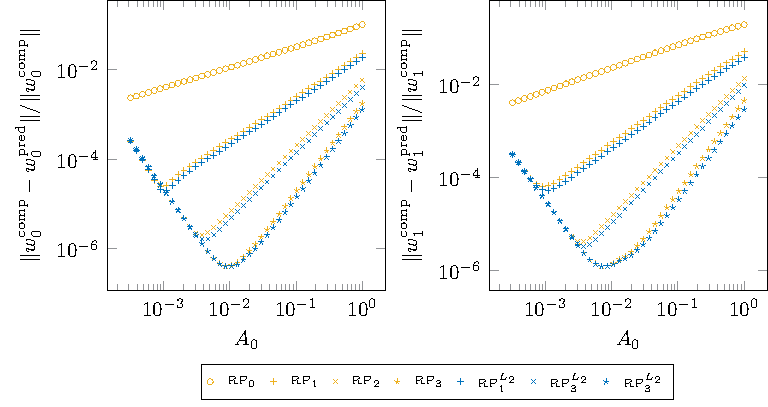
\includegraphics{\imagesdir/BTParameterdependentnormalformConvergencePlotRPMvsRPM.pdf}
    \caption{Log-log convergence plot comparing the different phase conditions
        when using the regular perturbation method (RP) for approximation the
        homoclinic solutions. The subscript in RP$_i$, $0\leq i \leq 3$, refers
        to the approximation order. The superscript $L_2$ refers to the phase
        condition \cref{eq:u_i_L2_phase_condition}. We observe here the standard V
        shaped graphs due to roundoff error.} 
    \label{fig:RP_vs_RPL2}
\end{figure}

In this example we compare five different methods to approximate the homoclinic
solution present in the universal unfolding \cref{eq:universal_unfolding}: 
\begin{itemize}
    \item the regular perturbation method, 
    \item the regular perturbation method with $L_2$ phase condition,
    \item the Lindstedt-Poincar\'e method without a higher-order time
        approximation as in~\cite{Al-Hdaibat2016},
    \item the Lindstedt-Poincar\'e method with a higher-order time
        approximation as derived here, 
    \item and the Lindstedt-Poincar\'e method with a different phase condition.
\end{itemize} 

In \cref{fig:RP_vs_RPL2} a log-log convergence plot is shown comparing the
asymptotics derived in~\cite{Al-Hdaibat2016} using the regular perturbation
method with phase condition $\dot u = 0$ against the asymptotics derived here
with the phase condition given in \cref{eq:u_i_L2_phase_condition}.  On the
abscissa is the amplitude $A_0$ and on the ordinate is the relative error
$\delta$ between the components $w_0$ and $w_1$ of the predicted solution and
the Newton corrected solution. We see that the $L_2$ phase condition is
slightly, but noticeably, more accurate at each order, confirming the geometric
intuition.

Next, we compare the regular perturbation method with the Lindstedt-Poincar\'e
method to approximate the homoclinic solution in log-log plot in
\cref{fig:RP_vs_LP2016_vs_LP}.  It is seen that the first order regular
perturbation method slightly outperforms the Lindstedt-Poincar\'e method, while
for the second and third-order the Lindstedt-Poincar\'e method  are clearly
better approximations than the regular perturbation method.  The third-order
approximation by the Lindstedt-Poincar\'e method without including a
higher-order approximation of the non-linear time transformation results in the
same order of accuracy as the zeroth-order regular perturbation method.

\begin{figure}
    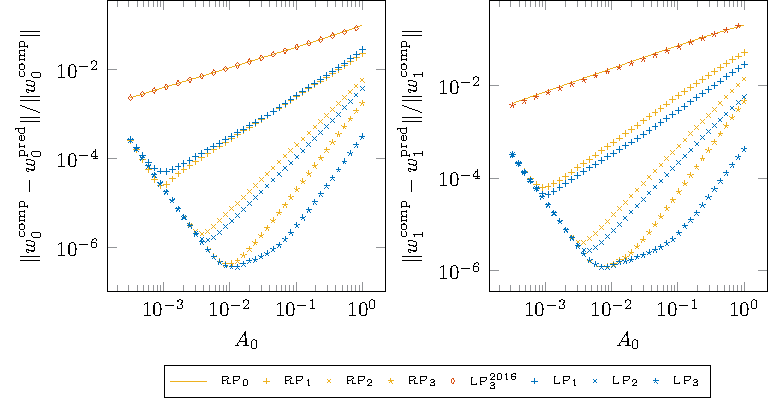
\includegraphics{\imagesdir/BTParameterdependentnormalformConvergencePlot.pdf}
    \caption{Log-log convergence plot comparing the relative errors of the computed
        homoclinic $w_0$ and $w_1$ component with the predicted solution in the
        topological normal form using four different methods: Regular
        Perturbation ($RP$, yellow), Lindstedt-Poincar\'e without higher-order time
        approximation ($LP_3^{2016}$, red), and Lindstedt-Poincar\'e combined
        with higher-order time approximation ($LP$, blue).}
    \label{fig:RP_vs_LP2016_vs_LP}
\end{figure}

It is thus essential to include a higher-order approximation of the non-linear
time transformation. To make it even more clear, we plotted the profiles of the
third-order approximations using the Lindstedt-Poincar\'e method as
in~\cite{Al-Hdaibat2016}, the regular perturbation method, and the
Lindstedt-Poincar\'e, together with the Newton corrected solutions in
\cref{fig:RP_vs_LP2016_vs_LP_profiles}. We see that the Lindstedt-Poincar\'e
method as in~\cite{Al-Hdaibat2016} approximates the solution rather poorly,
whereas the approximation derived in
\cref{sec:third_order_homoclinic_approximation_LP} is very accurate. Note that
when plotting these homoclinic approximations and corrections in $(w_0,w_1)$
phase-space, this difference is not visible at all. This explains why this has been
unnoticed in~\cite{Al-Hdaibat2016}.

\begin{figure}[!ht]
\centering
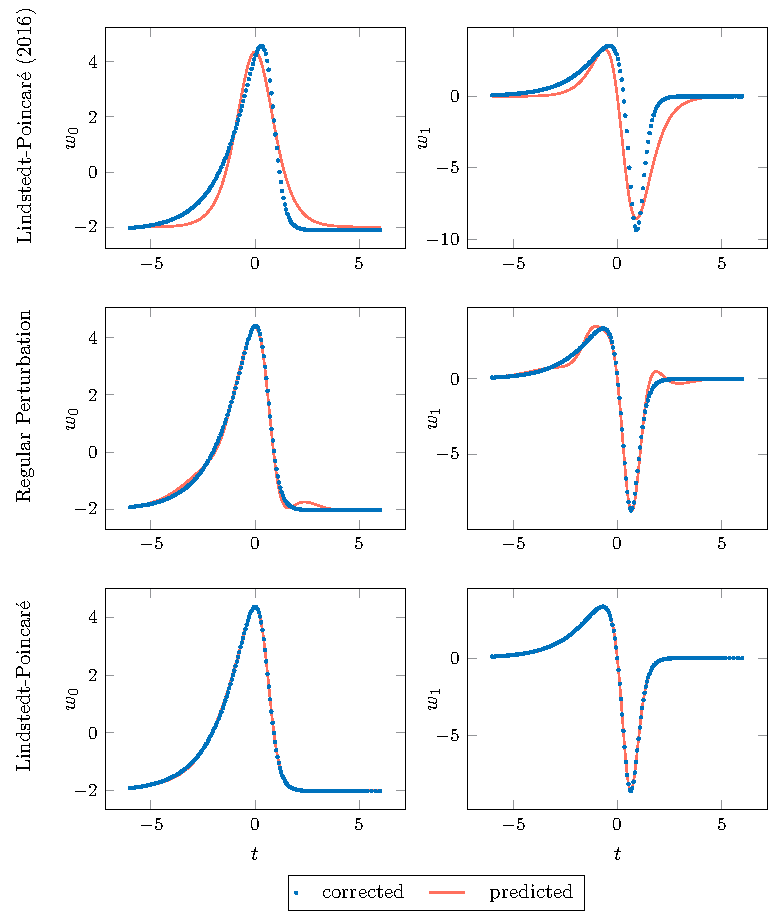
\includegraphics{\imagesdir/BTParameterdependentnormalformCompareProfiles.pdf}
\caption{Comparison of the profiles of the predicted and corrected
    homoclinic orbit for \cref{eq:universal_unfolding} using different
    approximation methods, see
\cref{sec:topological_normal_form} for a full description.}
\label{fig:RP_vs_LP2016_vs_LP_profiles}
\end{figure}

Lastly, we compare the two different phase conditions when using the
Lindstedt-Poincar\'e method in a log-log plot, in \cref{fig:LPM_vs_LPM}. It is
clearly seen that the phase condition used in \cref{sec:phase_condition}
improves, rather significantly, the accuracy of the third-order predictor.
However, in contrast with the different phase conditions used in the regular
perturbation method, we do not have any geometric (or analytical) explanation
for this improvement.

\begin{figure}
    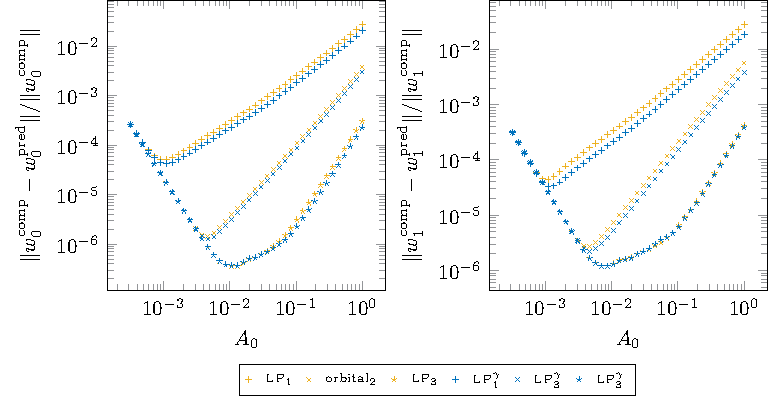
\includegraphics{\imagesdir/BTParameterdependentnormalformConvergencePlotLPMvsLPM.pdf}
    \label{fig:LPM_vs_LPM}
    \caption{
        Log-log convergence plot comparing the relative errors of the computed
        homoclinic $w_0$ and $w_1$ component with the predicted solution in the
        topological normal form using Lindstedt-Poincar\'e with two different
        phase-condition, see \cref{sec:phase_condition}.}
\end{figure}
Notice that here we do not compare the homoclinic predictors derived with
different normal forms. Indeed, when considering the universal unfolding
\cref{eq:universal_unfolding} the normal forms coincide, resulting in identical
predictors.


\ifthesis
\subsection{Hodgking-Huxley equations}

The Hodgkin-Huxley equations~\cite{HodgkinHuxley1952} relate the difference in electric
potential across the cell membrane $V$ and gating variables $m, n$ and $h$
for ion channels to the stimulus intensity $I$ and temperature $T$, as
follows:
\begin{equation}
\label{eq:HodgkinHuxleyEquations}
\begin{cases}
\begin{aligned}
    \dot{V} &= -G(V, m, n, h)+I, \\
    \dot{m} &= \Phi(T)\left[(1-m) \alpha_{m}(V)-m \beta_{m}(V)\right], \\
    \dot{n} &= \Phi(T)\left[(1-n) \alpha_{n}(V)-n \beta_{n}(V)\right], \\
    \dot{h} &= \Phi(T)\left[(1-h) \alpha_{h}(V)-h \beta_{h}(V)\right],
\end{aligned}
\end{cases}
\end{equation}
where 
\begin{align*}
    \Phi(T) & = 3^{({T}-6.3) / 10}, \\
    G(V, m, n, h) & =\bar{g}_{\mathrm{Na}} m^{3}
    h\left(V-\bar{V}_{\mathrm{Na}}\right)+\bar{g}_{\mathrm{K}}
    n^{4}\left(V-\bar{V}_{\mathrm{K}}\right)+\bar{g}_{\mathrm{L}}\left(V-\bar{V}_{\mathrm{L}}\right).
\end{align*}
The equations modeling the variation of membrane permeability are:
\begin{align*}
    \alpha_{m}(V) =& \Psi\left(\frac{V+25}{10}\right), & \beta_{m}(V) &= 4 e^{V / 18}, \\
    \alpha_{n}(V) =& 0.1 \Psi\left(\frac{V+10}{10}\right), & \beta_{n}(V) &= 0.125 e^{V / 80}, \\
    \alpha_{h}(V) =& 0.07 e^{V / 20}, & \beta_{h}(V) &= \left(1+e^{(V+30) / 10}\right)^{-1},
\end{align*} with
\begin{equation*}
    \Psi(x) = \begin{cases}
        x /\left(e^{x}-1\right), & \text { if } x \neq 0, \\
        1, & \text { if } x=0.
    \end{cases}
\end{equation*}
The parameters $\bar{g}_{\text{ion}}$ and $\bar{V}_{\text{ion}}$ representing
maximum conductance and equilibrium potential for the ion were obtained from
experimental data by Hodgkin and Huxley, with the values given below:
\[
\begin{array}{lll}
\bar{g}_{\mathrm{Na}}=120 \mathrm{mS} / \mathrm{cm}^{2}, 
& \bar{g}_{\mathrm{K}}=36 \mathrm{mS} / \mathrm{cm}^{2}, 
& \bar{g}_{\mathrm{L}}=0.3 \mathrm{mS} / \mathrm{cm}^{2}, \\
\bar{V}_{\mathrm{Na}}=-115 \mathrm{mV},
& \bar{V}_{\mathrm{K}}=12 \mathrm{mV}, 
& \bar{V}_{\mathrm{L}}=10.599 \mathrm{mV}.
\end{array}
\]
The values of $\bar{V}_{\mathrm{Na}}$ and $\bar{V}_{\mathrm{K}}$ can be
controlled experimentally~\cite{HodgkinHuxley1952a,Jack1975ElectricCurrentFlow}.
The temperature is set to $T=6.3^{\circ}$.

It is easy to see that the equilibria of \cref{eq:HodgkinHuxleyEquations} can be
parametrized by $V$
\begin{equation*}
    \begin{aligned}
        I(V) &= G(V, m(V), n(V), h(V)) \\
        y(V) &= \alpha_y(V)/(\alpha_y(V)+\beta_y(V)),
    \end{aligned}
\end{equation*}
where $y\in\{m,n,h\}$, see also~\cite{Guckenheimer@1993}. By calculating the Jacobian $A$ of
\cref{eq:HodgkinHuxleyEquations} at the equilibrium, we can derive the
characteristic polynomial $\rho_A(\lambda)$. The equation $\rho_A(0)=0$ can be
solved analytically for $\bar V_K$. Using this solution for $\bar V_k$ and
plotting the curve $\rho'(0)$ reveals two potential candidates for Bogdanov--Takens
points. Inspecting the geometric multiplicity of these two points narrows the
possibilities down to the point
\begin{equation}
\label{eq:HodgkinHuxleyBTpoint}
\begin{pmatrix}
    V \\m \\n \\h \\ \bar V_k \\ I 
\end{pmatrix}
\approx
\begin{pmatrix}
-2.835463618170097 \\ 0.07351498630356315 \\ 0.361877602925177 \\ 0.494859128785482 \\
-4.977020454108788 \\ -0.06185214966177632
\end{pmatrix}.
\end{equation}  
Inspecting the coefficients of the normal form shows that
\[
a = 2.5515\cdot 10^{-5}, \qquad b =  -0.0075.
\] 
Thus, provided the transversality conditions are satisfied, we can use \MATCONT to
start continuation of the homoclinic orbits emanating from this point.

\begin{figure}
    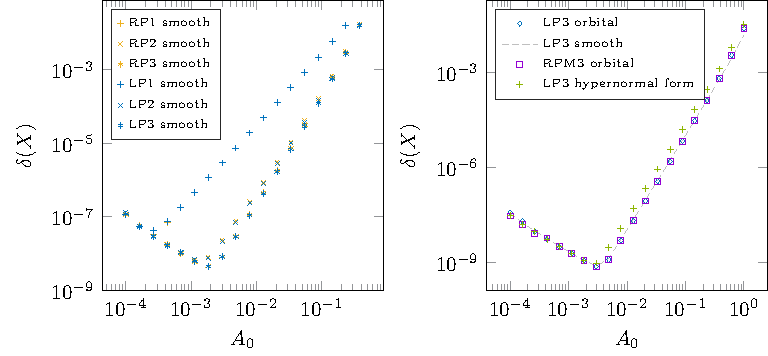
\includegraphics{\imagesdir/HodgkinHuxleyConvergencePlotFull.pdf}
    \caption{Convergence plot for the homoclinic predictors near the
    Bogdanov--Takens bifurcation \cref{eq:HodgkinHuxleyBTpoint} in the
    Hodgkin-Huxley equations \cref{eq:HodgkinHuxleyEquations}.}
    \label{fig:HodgkinHuxleyConvergencePlot}
\end{figure}

In \cref{fig:HodgkinHuxleyConvergencePlot} there are two log-log convergence
plots shown. Note that in this and the next example, we show the relative error
$\delta(X)$ between the predicted and corrected Newton solution to the defining
system \cref{eq:definingSystem}.  In the left plot (a) we compare the regular
perturbation method with the Lindstedt-Poincar\'e method. We see that compared
with the previous example, the Lindstedt-Poincare\'e method is slightly less
accurate than the regular perturbation method and the second-order.
Nevertheless, we clearly see that the order of convergence lifts from the
normal form to the two-dimensional center manifold in $\mathbb R^4$. In the
plot right (b) we compare four different third approximations to the homoclinic
orbit
\begin{itemize}
    \item the Lindstedt-Poincar\'e method using the smooth orbital normal form
        (the blue diamond),
    \item the Lindstedt-Poincar\'e method using the smooth normal form
        (the dashed light gray line),
    \item the regular perturbation method using the smooth normal form
        (the pink square), 
    \item the Lindstedt-Poincar\'e method using the hyper-normal form
        (the green plus).
\end{itemize}

We see that both the Lindstedt-Poincar\'e method and the regular perturbation
method using the smooth orbital normal form are in perfect agreement with the
Lindstedt-Poincar\'e method using the smooth normal form. Only the homoclinic
predictor using the hyper-normal form is slightly less accurate.
\fi

\subsection{Homoclinic RG flows}
In~\cite{Jepsen2021HomoclinicRG} an $\mathcal N = 1$ supersymmetric model of interacting
scalar superfields $\Phi_{ab}^i$ that is invariant under the action of an $O(N)
\times O(M)$ group in $d = 3 - \epsilon$ dimensions is considered.
The coupling constants $g_i(i=1,\dots,4)$ satisfy the following differential
equations
\begin{equation}
    \label{eq:HomoclinicRGflows}
    \dot g = -\epsilon g + \beta^{(2)}(g,M,N) + \mathcal O(g^5),  \qquad g\in\mathbb R^4,
\end{equation} 
where the two-loop contributions $\beta_i^{(2)}(i=1,\dots,4)$ are cubic in the
coupling and the parameter $\epsilon$ is scaled to $1$.  The exact expression for
$\beta_i^{(2)}$ are quite long can be found in~\cite[Appendix B]{Jepsen2021HomoclinicRG}
or in the \href{https://mmbosschaert.github.io/MatCont7p2NewInitBTHom-/}{online Jupyter
Notebook}.
\begin{figure}[b!]
    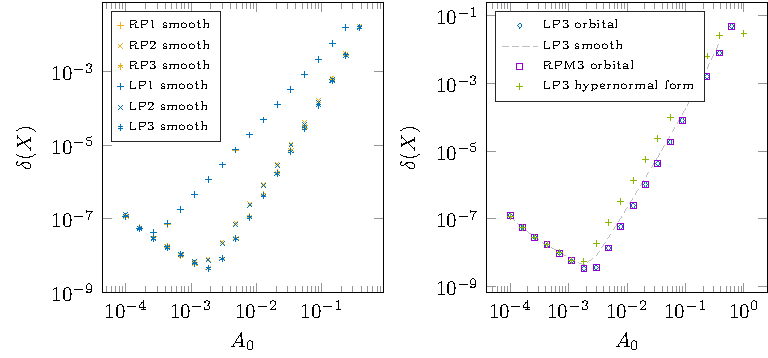
\includegraphics{\imagesdir/HomoclinicRGFlowsConvergencePlotFull.pdf}
    \caption{Convergence plot for the homoclinic predictors near one of the
        two Bogdanov--Takens bifurcation in the Homoclinic RG flows model 
        \cref{eq:HomoclinicRGflows}.}
    \label{fig:HomoclinicRGFlowsConvergencePlot}
\end{figure}
%
\begin{figure}[t!]
    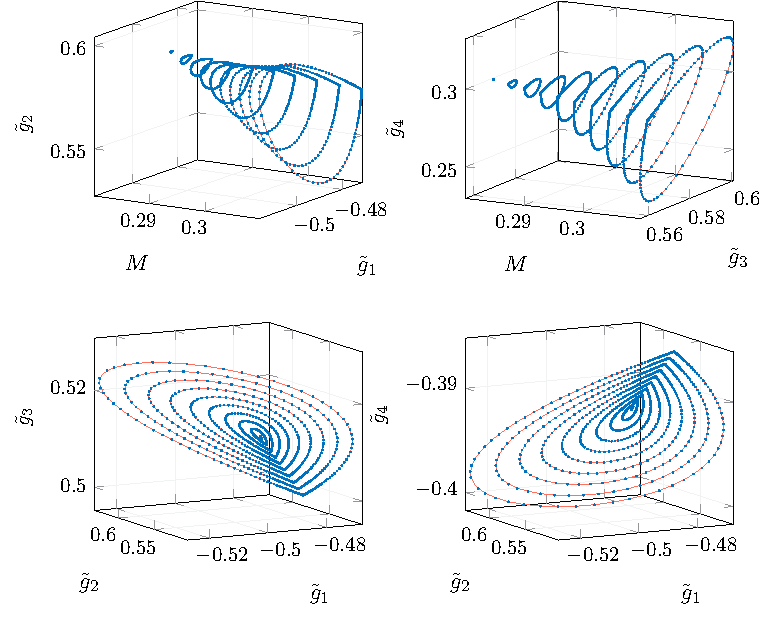
\includegraphics{\imagesdir/HomoclinicRGflowsCompareOrbits3D_LP.pdf}
    \caption{Comparison between the predicted (solid, red) with the corrected
        (dotted, blue) homoclinic orbits using the Lindstedt-Poincar\'e method
        with the smooth orbital normal form for amplitudes $A_0 = 10^{-3}$ to
        $A_0=10^{-1}$. The $g_i(i=1,\dots,4)$ coordinates have been rotated and stretched
        to make the homoclinic orbits better visible.}
    \label{fig:HomoclinicRGFlows}
\end{figure}
%
\ifthesis
\begin{figure}[t!]
\includetikzscaled{HomoclinicRGflowsCompareParameters}
\caption{Comparison between the computed homoclinic bifurcation curve
    (solid, blue) with the predicted values in parameter-space $(M,N)$.
    The yellow crosses are the second-order predictor obtained with the
    transformation as given in {\cite{Al-Hdaibat2016}}. The blue plus
    signs are the second-order predictor obtained in this \paper{}. These are
    indistinguishable at this scale from the third-order
    predictor (dotted, red) obtained in this \paper{}.}
\label{fig:HomoclinicRGFlowsParameters}
\end{figure}
\fi

In~\cite{Jepsen2021HomoclinicRG} a Bogdanov--Takens point near the parameter values
$M=0.2945$ and $N = 4.036$ is located. Using these parameter values we locate an
equilibrium at 
\[
\begin{pmatrix}
    g_1 \\ g_2 \\ g_3 \\ g_4
\end{pmatrix} = 
\begin{pmatrix}
    0.0701457361241472 \\ -0.06520883770451065 \\ 0.001823543197553845 \\ 0.22874527306411319
\end{pmatrix}.
\]
By continuing the equilibrium in the parameter $M$ we detect several limit
points and two Hopf points. We continue the second Hopf point at $M\approx0.2958$ 
in parameters $M$ and $N$. Several Bogdanov--Takens points are detected. The
first Bogdanov--Takens point is located at
\[
\begin{pmatrix}
    g_1 \\ g_2 \\ g_3 \\ g_4 \\ 
\end{pmatrix} = 
\begin{pmatrix}
    -0.715157316845187 \\ -0.250968103603174 \\ 0.510051114588271 \\ -0.391935453715783 \\
\end{pmatrix},
\]
with parameter values
\[
    (M, N) = (0.294477255737036, 4.035536108506390).
\]

\ifthesis 
In \cref{fig:HomoclinicRGFlowsConvergencePlot} we have created similar log-log
convergence plots as in the previous example. The plots look very alike.
%
Lastly, in \cref{fig:HomoclinicRGFlows}  we compare the predicted (solid, red)
with the corrected (dotted, blue) homoclinic orbits using the
Lindstedt-Poincar\'e method with the smooth orbital normal form for amplitudes
$A_0 = 10^{-3}$ to $A_0=5\times 10^{-2}$. We see that they are in excellent
agreement. In \cref{fig:HomoclinicRGFlowsParameters} we compared the
    computed homoclinic bifurcation curve (solid, blue) with the predicted
    values in parameter-space $(M, N)$. Most important to notice here is that
    the predictor given in \cite{Al-Hdaibat2016} (the yellow crosses) is less
accurate than the second-order predictor (blue plus signs) obtained in this
\paper{}. 
\else
In \cref{fig:HomoclinicRGFlowsConvergencePlot} there are two log-log
convergence plots shown. Note that in this and the example in
\cref{sec:Hodgking-Huxley}, we show the relative error $\delta(X)$ between the
predicted and corrected Newton solution to the defining system
\cref{eq:definingSystem}.  We clearly see that the order of convergence
correctly lifts from the normal form to the two-dimensional center manifold in
$\mathbb R^4$. In the left plot we compare the regular perturbation method
with the Lindstedt-Poincar\'e method. We see that these are almost
indistinguishable. In the plot right we compare four different third
approximations to the homoclinic orbit
\begin{itemize}
    \item the Lindstedt-Poincar\'e method using the smooth orbital normal form
        (the blue diamond),
    \item the Lindstedt-Poincar\'e method using the smooth normal form
        (the dashed light gray line),
    \item the regular perturbation method using the smooth normal form
        (the pink square), 
    \item the Lindstedt-Poincar\'e method using the hyper-normal form
        (the green plus).
\end{itemize}

We see that both the Lindstedt-Poincar\'e method and the regular perturbation
method using the smooth orbital normal form are slightly more accurate then the
Lindstedt-Poincar\'e method using the smooth normal form. The homoclinic
predictor using the hyper-normal form is less accurate compared to be
other methods.

Lastly, in \cref{fig:HomoclinicRGFlows}  we compare the predicted (solid, red)
with the corrected (dotted, blue) homoclinic orbits using the
Lindstedt-Poincar\'e method with the smooth orbital normal form for amplitudes
$A_0 = 10^{-3}$ to $A_0=5\times 10^{-2}$. We see that they are in excellent
agreement. In \cref{fig:HomoclinicRGFlowsParameters} we compared the
    computed homoclinic bifurcation curve (solid, blue) with the predicted
    values in parameter-space $(M, N)$. Most important to notice here is that
    the predictor given in \cite{Al-Hdaibat2016} (the yellow crosses) is less
accurate than the second-order predictor (blue plus signs) obtained in this
\paper{}. 
\fi

\section{Discussion}%
We have derived third-order predictors for the homoclinic curve emanating from
the generic codimension two Bogdanov--Takens bifurcation in general
$n$-dimensional autonomous ODEs. By considering the smooth orbital normal form
\cref{eq:normal_form_orbital} and incorporating the time-re\-pa\-ram\-e\-triza\-tion in the
homological equation \cref{eq:homological_equation}, we were able to derive
the third-order asymptotic of the homoclinic curve independent of any undetermined
normal form coefficients. However, for this simplification, there is a price to
pay. Firstly, the systems to be solved to obtain the coefficients for the
parameter-dependent center manifold become more difficult, see
\cref{subsec:center_manifold_tranformation_orbital}. Ideally, there should be
an automatic algorithm in line with~\cite{Murdock@2003}. However, to the best
of our knowledge, such algorithms do not exist yet.  Secondly, the translation
of time in the homological equation needs to be inverted numerically. This,
however, can be done relatively cheap and is very accurate, as shown by the
examples.

In \cref{thm:coefficients} we have shown how to obtain a correct transformation
to the parameter-dependent center manifold by inspecting which terms are in,
\emph{and are not in}, the normal form that alters the homoclinic asymptotic up
to certain order. The examples in \cref{sec:examples}, the
\hyperref[mysupplement]{online Supplement}, and the
\href{https://mmbosschaert.github.io/MatCont7p2NewInitBTHom-/}{online Jupyter
Notebook}, but also the comparison in
\cref{sec:comparison_homoclinic_predictors}, confirm that we indeed have
obtained the correct transformation.

The additional non-linear transformation
\cref{eq:second_time_transformation} greatly simplifies the computation
of the coefficients in the Lindstedt-Poincar\'e method since all calculations
become essentially polynomial, which is ideal for computers to work with.
Nonetheless, the algorithmic complexity grows exponentially as the order
increases linearly. Also, the radius of convergence is clearly finite, as shown
in \cref{sec:case_study_BT2}. One way to increase the convergence radius is by
using transformations as in~\cite{Milton@1974}. However, we didn't include any
results in this direction since it would distract too much from our main
objectives.

Using different phase conditions can improve the accuracy of the homoclinic
approximation. However, this only holds true when applied directly to the system
considered. Indeed, the phase condition isn't invariant under the
parameter-dependent center manifold transformation. Thus, its applicability is
very limited. Furthermore, using a different phase condition may, somewhat
unexpectedly, result in difficult integrals to be solved, see
\cref{sec:RPM_norm_minimizing_phase condition}.

The higher-order approximation to the non-linear time transformation in the
Lindstedt-Poincar\'e method turns out to be essential to obtain higher-order
approximations to the homoclinic solutions. This is clearly seen by inspecting
the profiles of the homoclinic solution in
\cref{fig:RP_vs_LP2016_vs_LP_profiles} and in the convergence plot in
\cref{fig:RP_vs_LP2016_vs_LP}. Without the higher-order approximation the same
convergence order as the unperturbed Hamiltonian solution, i.e., the
zeroth-order solution. It should be noted that the higher-order approximation
of the non-linear time transformation is more difficult to obtain. Therefore,
we conclude that there seem to be \emph{no benefits} of the
Lindstedt-Poincar\'e method over the regular perturbation method for starting
continuation of homoclinic orbits. Indeed, the numerical comparisons in
\cref{sec:examples} show similar accuracy of convergence at each order.

By comparing the convergence order of Lindstedt-Poincar\'e the with the regular
perturbation method, we see that contrary to what one might expect, the
regular perturbation method may result in better accuracy at the same order. A
possible explanation for this might be that although the Lindstedt-Poincar\'e
method provides a uniform approximation in time, the numerical solution is
truncated to a finite interval in which the `parasitic turn' doesn't give a
significant contribution. After all, it then simply depends on the higher-order
non-linear terms in the system which favor one method over the other. 


\section*{Acknowledgments}
The authors would like to thank Prof. Peter De Maesschalck (Hasselt University,
Belgium) for multiple useful discussions during this research project, Prof.
Wolf-J\"urgen Beyn (Bielefeld University, Germany) for his positive comments on
the preprint, and Dr. Hil Meijer (University of Twente, The Netherlanda) for
multiple suggestions leading to a significant improvement of the \paper{}.


\begin{subappendices}
\section{Explicit example demonstrating incorrect predictor}
\label{app:incorrect_predictor}

Although the second-order homoclinic approximation derived
in~\cite{Al-Hdaibat2016} for the smooth normal form \cref{eq:BT_smooth_nf} is
correct, the parameter and center manifold transformation are incorrect. To see
this, we suppose \cref{eq:ODE} is given by
\begin{align}
\label{eq:btnormalform_with_alpha2^3}
\dot x = f(x,\alpha) = \begin{pmatrix}   x_1 \\
 \alpha_1 + \alpha_2 x_1 + x_0^2 + x_0 x_1 + c_1 \alpha_2^3
 \end{pmatrix},
\end{align}
for some arbitrary nonzero constant $c_1 \in \mathbb R$.  We will now compare
two different methods for obtaining a second-order approximation to the
homoclinic solution in \cref{eq:btnormalform_with_alpha2^3}. To keep the
exposition as clear as possible, we focus solely on the parameters. For the
first method we directly apply the singular rescaling 
\[
\alpha_1=-4\epsilon^4, \quad \alpha_2 = \eta \epsilon^2,
\quad x_0= \epsilon^2, \quad x_1= \epsilon^3, \quad
s=\epsilon t,
\]
to \cref{eq:btnormalform_with_alpha2^3}. This yields the system
\[
\begin{cases}
\begin{aligned}
  \dot u ={}& v, \\
  \dot v ={}& -4 + u^2 + v\left( u + \tau \right)\epsilon +  c_1 \tau^3
	\epsilon^2, \\
\end{aligned}
\end{cases}
\]
where the dot $\dot{}$ now represents the derivative with respect to $s$.
Then, using the generalized Lindstedt-Poincar\'e method we obtain the approximation
\begin{equation}
\label{eq:first_predictor}
				(\alpha_1, \alpha_2) = \left(-4 \epsilon^4, \frac{10}7 \epsilon^2 
+\frac{288-1250 c_1}{2401}\epsilon^4 + \mathcal O(\epsilon^5) \right)
\end{equation}
for the parameters. For the second method we use the predictor
from~\cite{Al-Hdaibat2016}. That is, we use the second-order homoclinic
predictor derived for the smooth normal form \cref{eq:BT_smooth_nf}. Then
calculate the center manifold transformation, which for the two-dimensional
systems reduces to a near-identity transformation, and parameter transformation
to transfer the predictor to the original system. We obtain that the near-identity
and parameter transformation are just the identities. Thus, we obtain the
predictor
\begin{equation}
				\label{eq:second_predictor}	
				(\alpha_1, \alpha_2) = \left(-4 \epsilon^4, \frac{10}7 \epsilon^2 
				+\frac{288}{2401}\epsilon^4 + \mathcal O(\epsilon^5) \right).
\end{equation}
Obviously, this result is wrong.  To see why the latter second predictor
doesn't contain the term $c_1$ we consider the near-identity transformation
\begin{align}
\label{eq:near_identity_tranformation}
  \begin{cases}
  \begin{aligned}
    x &{}= w, \\ 
    \alpha &{}= \beta+ \begin{pmatrix} -c_1 \\ 0 \end{pmatrix}\beta_2^3.
  \end{aligned}
  \end{cases}
\end{align}
Then system \cref{eq:btnormalform_with_alpha2^3} becomes
\begin{align*}
  \begin{cases}
  \begin{aligned}
     \dot w_0 &{}= w_1, \\
		 \dot w_1 &{}= \beta_1 + \beta_2 w_1 + w_0^2 + w_0 w_1.
  \end{aligned}
  \end{cases}
\end{align*}
Using the second-order predictor from~\cite{Al-Hdaibat2016} for the smooth
normal form we obtain
\[
    (\beta_1, \beta_2) = \left(-4 \epsilon^4, \frac{10}7 \epsilon^2 
    +\frac{288}{2401}\epsilon^4 + \mathcal O(\epsilon^5) \right).
\]
Then using the near-identity transformation
\cref{eq:near_identity_tranformation} yields the predictor
\begin{equation*}
				(\alpha_1, \alpha_2) = \left(-4 \epsilon^4 
								- c_1 \left(\frac{10}7 \epsilon^2 
								+\frac{288}{2401}\epsilon^4 + \mathcal O(\epsilon^5) \right)^3, 
								\frac{10}7 \epsilon^2 
				+\frac{288}{2401}\epsilon^4 + \mathcal O(\epsilon^5) \right).
\end{equation*}
To compare this predictor with \cref{eq:first_predictor} we eliminate $\epsilon$
in both equations. This yields
\begin{equation*}
				\alpha_2(\alpha_1) = - \frac57 \sqrt{-\alpha_1} +
				\frac{288-1250c_1}{2401} \alpha_1 + \mathcal O(\alpha_1^{\frac32}).
\end{equation*}

We conclude, as expected, that if the correct transformation is used between the
normal form and the original system, we keep the correct order of accuracy for
the approximation. In~\cite{Al-Hdaibat2016} the coefficients $H_{0003}$ and
$K_{03}$ (among other coefficients) are not incorporated into the
parameter-dependent center manifold transformation
\cref{eq:H_expansion,eq:K_expansion} leading to the incorrect
predictor \cref{eq:second_predictor}.

\section[Integrals from section 2.3.1]{Integrals from
\texorpdfstring{\cref{sec:third_order_homoclinic_approximation_RP}}{subsection 3.1.1}}%
%TODO : check is the hard coded reference is up-to-date.
\label{sec:I_n}
Making the substitution $s=\log(u)$ in \cref{eq:I_n} yields
\begin{equation*}
    I_n = 2^n \int_1^\infty \log^3\left(\frac{u^2+1}{u}\right) \frac{u^{n-1}}{(u^2+1)^n} \, du.
\end{equation*}
Then, by making the reciprocal substitution $u \to \frac{1}{u}$, we can show
that
\begin{equation*}
    I_n = 2^{n-1} \int_0^\infty \log^3\left(\frac{u^2+1}{u}\right)
            \frac{u^{n-1}}{(u^2+1)^n} \, du.
\end{equation*}
The last integral can be separated into the four following integrals
\begin{align}
    I_n^{(1)} =& \int_0^\infty \log^3(u^2+1) \frac{u^{n-1}}{(u^2+1)^n} du
              \label{eq:In1}, \\
    I_n^{(2)} =& \int_0^\infty \log^2(u^2+1)\log u \frac{u^{n-1}}{(u^2+1)^n} du 
              \label{eq:In2}, \\
    I_n^{(3)} =& \int_0^\infty \log(u^2+1)\log^2 u \frac{u^{n-1}}{(u^2+1)^n} du 
              \label{eq:In3}, \\
    I_n^{(4)} =& \int_0^\infty \log^3 u \frac{u^{n-1}}{(u^2+1)^n} du
              \label{eq:In4}.
\end{align}
The integral \cref{eq:In1} can easily be solved by first applying the
substitutions $u\to u^2+1$ and $u\to\frac1u$ consecutively to obtain
\begin{align*}
    I_n^{(1)} 
    &{}= - \frac12 \int_0^1 \log^3 (u) 
        \left(1-u\right)^{\frac{n}{2}-1}u^{\frac{n}{2}-1} \, du.
\end{align*}
Then using the binomial theorem yields
\begin{equation*}
    I_n^{(1)} 
= - \frac12 \sum_{k=0}^{\frac{n}{2}-1} \binom{\frac{n}{2}-1}k (-1)^k 
            \int_0^1 \log^3 (u) u^{\frac{n}{2}-1+k} \, du
    = \frac12 \sum_{k=0}^{\frac{n}{2}-1} \binom{\frac{n}{2}-1}k
    \frac{(-1)^k 3!}{({\frac{n}{2}+k})^4},
\end{equation*}
where in the last equality we used the well-know identity
\begin{equation}
    \label{eq:int01umlogn}
    \int_0^1 u^m \log^n (u) \, du = (-1)^n \frac{n!}{(m+1)^{n+1}},
\end{equation}
for $n$ and $m$ natural numbers.

To solve the integral \cref{eq:In2} we make three consecutive
substitutions: $u\to u^2$, $u\to u-1$, and $u\to\frac{1}{u}$. This gives
\[
    I_n^{(2)}=
    -\frac{1}{4} \int_0^1 
        \left(\log^3(v)-\log^2(v)\log(1-v) \right) 
        (1-v)^{\frac{n}2-2} v^{\frac{n}2-1} dv. \\
\]
Then, by using the binomial theorem and expanding the logarithm we obtain
\ifsiam
\begin{multline*}
    I_n^{(2)}={}
\frac{1}{4} \sum_{k=0}^{\frac{n}{2}-1} \binom{\frac{n}{2}-1}k
        (-1)^k \left[ 
          \int_0^1 \log^3(v) (1-v)^{\frac{n}2-2} v^{\frac{n}2-1} dv \right. \\
        \left. 
        -\sum_{l=1}^\infty \frac1l \int_0^1 \log^2(v) v^{\frac{n}2-1+k+l} dv 
    \right].
\end{multline*}
\else
\begin{multline*}
    I_n^{(2)}={}
\frac{1}{4} \sum_{k=0}^{\frac{n}{2}-1} \binom{\frac{n}{2}-1}k
        (-1)^k \left[ 
          \int_0^1 \log^3(v) (1-v)^{\frac{n}2-2} v^{\frac{n}2-1} dv
        -\sum_{l=1}^\infty \frac1l \int_0^1 \log^2(v) v^{\frac{n}2-1+k+l} dv 
    \right].
\end{multline*}
\fi
Using equality \cref{eq:int01umlogn} once more yields
\begin{equation*}
    I_n^{(2)}={}
\frac{1}{4} \sum_{k=1}^{\frac{n}{2}-1} \binom{\frac{n}{2}-1}k
    (-1)^k \left[ \frac{3!}{(\frac{n}{2}+k)^4}
     -2\sum_{l=1}^\infty \frac1{l(\frac{n}2+k+l)^3}\right].
\end{equation*}
Fractional decomposition shows that the innermost summation in the last
equation is equal to 
\begin{equation*}
    \sum_{l=1}^\infty \frac1{l(\frac{n}2+k+l)^3}
        = \frac{8}{2k+n} \left(\frac{H_{\frac{n}{2} + k}}{(2k+n)^2} +
            \frac{H^{(2)}_{k+\frac{n}{2}} - \zeta(2)}{2(2k+n)} +
            \frac{H^{(3)}_{k+\frac{n}{2}} - \zeta(3)}4 
        \right).
\end{equation*}
%
Thus, the integral in \cref{eq:In2} is equal to
\begin{multline*}
    I_n^{(2)} = \frac{1}{4} \sum_{k=1}^{\frac{n}{2}-1} 
        \binom{\frac{n}{2}-1}k (-1)^k 
        \left[ \frac{3!}{(\frac{n}{2}+k)^4} \right.  
        - \frac{2}{2k+n} 
            \left(\frac{4}{(2k+n)^2} H_{\frac{n}{2}+k} \right. \\ 
            \left.\left. + \frac{2}{(2k+n)} H^{(2)}_{\frac{n}{2}+k} 
            + H^{(3)}_{\frac{n}{2}+k} - \frac{2\zeta(2)}{2k+n} - 4\zeta(3)
    \right)\right].
\end{multline*}
%
Now most work is done, since subtracting two times \cref{eq:In2} from
\cref{eq:In3} is equal to
\begin{equation*}
    \int_0^\infty \log^2(u^2+1)\log (u) \log\left(1+\frac{1}{u^2}\right)
        \frac{u^{n-1}}{(u^2+1)^n} du.
\end{equation*}
The reportorial substitution $u\to\frac{1}{u}$ shows that this integral
vanishes. The same substitution also shows that the integral in  \cref{eq:In4}
vanishes.  We thus obtain the closed-form expression 
\begin{multline*}
    I_n = 2^{n-3} 3 \sum_{k=0}^{\frac{n}{2}-1} \binom{\frac{n}{2}-1}k  
            (-1)^k  \\
        \left[\frac1{(\frac{n}{2}+k)^4} +
            \frac{8}{2k+n} \left(\frac{H_{\frac{n}{2} + k}}{(2k+n)^2}
                + \frac{H^{(2)}_{\frac{n}{2}+k} - \zeta(2)}{2(2k+n)}
            + \frac{H^{(3)}_{\frac{n}{2}+k} - \zeta(3)}{4}
        \right)\right],
\end{multline*}
where $\zeta$ is the Riemann zeta function and $H_n^{(m)}$ is the $n$-th
generalized harmonic number of order $m$.

\ifthesis
\section{Asymptotics for homoclinic solution in the smooth normal form}
\else
\subsubsection{Asymptotics for homoclinic solution in the smooth normal form}
\fi
\label{sec:asymptotics-for-homoclinic-solution-for-the-smooth-normal-form}
Following the procedure outlined in \cref{sec:PolynomailLindstedtPoincare} to
the second-order nonlinear differential equation
\cref{eq:second_order_nonlinear_oscillator_smooth_normalform} obtained from the
smooth normal form \cref{eq:BT_smooth_nf}. For the third-order homoclinic
predictor we obtain
\begin{align}
				\sigma ={}& 6 + \frac{3 \left(-70 a_1 b+6 b^2+49 d\right)}{49 a^2} \epsilon^2
                    + \mathcal{O}(\epsilon^4),
				\nonumber \\
				\delta ={}& -4 + \frac{140 a_1 b-18 b^2-245 d}{49 a^2} \epsilon^2
                    + \mathcal{O}(\epsilon^4),
				\nonumber \\
				\label{eq:tau_smooth}
				\tau   ={}& \frac{10}{7} + \frac{98 b (50 a b_1+73 d)-9604 a e-2450 a_1 b^2+288 b^3}{2401 a^2 b} \epsilon^2
								+ \mathcal{O}(\epsilon^4), \\
				\tilde \omega(\zeta) ={}& 1 - \frac{6b}{7a}\zeta  \epsilon	+ 
				\frac{70 a_1 b+18 b^2 \left(3 \zeta ^2+1\right)+49 d \left(9 \zeta ^2-5\right)}{196 a^2} \epsilon^2 +
				\nonumber \\
        & \frac{\zeta}{2401 a^3} \left( \left(-147 b \left(20 a b_1-7 d
        \zeta ^2+11 d\right)-9604 a e \left(\zeta ^2-1\right) \right. \right. \nonumber \\
        & \left. \left. +1470 a_1 b^2+18 b^3 \left(7 \zeta ^2-11\right)\right) \right)\epsilon^3 + \mathcal{O}(\epsilon^4)
        \nonumber.
\end{align}
It follows that
\begin{align}
    \label{eq:third_order_uhat_smooth}
    \tilde {u}(\zeta) 
    ={}& 6 \zeta ^2-4 + \frac{-70 a_1 b \left(3 \zeta ^2-2\right)+18 b^2 \left(\zeta
    ^2-1\right)+49 d \left(3 \zeta ^2-5\right)}{49 a^2} \epsilon^2 
        + \mathcal{O}(\epsilon^4), \\
    \label{eq:third_order_vhat_smooth}
	\tilde  v(\zeta) 
  ={}& -2 \tilde\omega(\zeta) \sigma (1-\zeta^2)\zeta
	= -\left[ -12 + \frac{72b}{7a} \zeta \epsilon
			 - \frac{3}{49 a^2} \left(70 a_1 b-6 b^2 \left(9 \zeta ^2+5\right)
       \right. \right. \\
     & \left. -147 d \left(3 \zeta ^2-1\right)\right)\epsilon^2 + \frac{12
         \zeta}{2401 a^3}  \left(147 b \left(20 a b_1-7 d \zeta ^2+18
         d\right) \right. \nonumber \\
    & \left. \left. + 9604 a e \left(\zeta ^2-1\right)-2940 a_1 b^2-18 b^3 \
\left(7 \zeta ^2-18\right)\right) \epsilon^3 \right]
     (1-\zeta^2) \zeta + \mathcal{O}(\epsilon^4) \nonumber.
\end{align}

The relation $\xi(s)$ can be obtained by solving the ODE
\begin{equation}
				\label{eq:third_order_dxi_ds_smooth}
				\frac{d\xi}{ds}(s) = \tilde \omega(\tanh(\xi(s))).
\end{equation}
Thus, we substitute 
\begin{equation*}
				\xi(s) = s + \xi_1(s)\epsilon + \xi_2(s)\epsilon^2
				+ \xi_3(s)\epsilon^3 + \mathcal{O}(\epsilon^4),
\end{equation*}
into \cref{eq:third_order_dxi_ds_smooth} and expand the resulting equation in
$\epsilon$ to obtain
\begin{align*}
\frac{d\xi_1}{ds}(s) ={}& -\frac{6b\tanh(s)}{7a}, \\
\frac{d\xi_2}{ds}(s) ={}& \frac{-168 a b \sech^2(s) \xi_1(s)+70 a_1 b+9 \left(6 b^2+49 d\right) \tanh ^2(s)+18 b^2-245 d}{196 a^2} , \\
\frac{d\xi_3}{ds}(s) ={}& \frac{\sech^3(s)}{4802 a^3} \left(4116 a^2 b \sinh (s) (\xi_1(s))^2-4116 a^2 b \cosh (s) \xi_2(s) \right. \\
                        & +441 a \left(6 b^2+49 d\right) \sinh (s)\xi_1(s)+2 \sinh (s) \left(-3 b \cosh (2 s) \right. \\
                        & \left(98 (5 a b_1+d)-245 a_1 b+12 b^2\right)-1470 a b b_1+9604 a e+735 a_1 b^2 \\
                        & \left. \left. -162 b^3-1323 b d\right)\right).
\end{align*}
Here we directly used that $\xi_0(s)=s$. By solving these equations recursively,
we obtain
\begin{equation*}
\begin{aligned}
\xi_1(s) ={}& - \frac{6b}{7a}\log(\cosh(s)), \\
\xi_2(s) ={}& \frac{2 s \left(35 a_1 b-36 b^2+98 d\right)+9 \tanh (s) \left(16 b^2 \log (\cosh (s))+10 b^2-49 d\right)}{196 a^2}, \\
\xi_3(s) ={}& \frac{1}{4802 a^3}\left(-7 \sech^2(s) \left(1372 a e-27 b \left(6 b^2+49 d\right) \log (\cosh (s)) \right. \right. \\
            & \left. +216 b^3 \log ^2(\cosh(s))-234 b^3-147 b d\right)-5880 a b b_1 \log (\cosh (s)) \\
            & + 9604 a e+42 b s \tanh (s) \left(-35 a_1 b+36 b^2-98 d\right)+4410 a_1 b^2 \log (\cosh (s)) \\
            & \left. -1656 b^3 \log (\cosh (s))-1638 b^3+2940 b d \log (\cosh (s))-1029 b d\right).
\end{aligned}
\end{equation*}
Here we used the phase condition that $\xi_i(0)=0,i=1,2,3$. This results in the
constraint $v(0)=0$. Substituting the above expression for $\xi$ into
\cref{eq:blowup_smooth} we obtain the third-order predictor
\begin{equation}
\label{eq:third_order_predictor_LP_tau_smooth}
\ifthesis
\begin{cases}
\begin{aligned}
w_0(t)  &= \frac{1}{a} \tilde{u}\left(\tanh\left(\xi(\epsilon t)\right)\right) \epsilon^2, \\
w_1(t)  &= \frac{1}{a} \tilde{v}\left(\tanh\left(\xi(\epsilon t)\right)\right) \epsilon^3, \\
\beta_1    &= -\frac{4}{a}\epsilon^4, \\
\beta_2    &= \frac{b}{a}\tau\epsilon^2,
\end{aligned}
\end{cases}
\else
\left( w_0(t), w_1(t), \beta_1, \beta_2 \right) = 
\left( 
\frac{1}{a} \tilde{u}\left(\tanh\left(\xi(\epsilon t)\right)\right) \epsilon^2, \\
\frac{1}{a} \tilde{v}\left(\tanh\left(\xi(\epsilon t)\right)\right) \epsilon^3, \\
-\frac{4}{a}\epsilon^4, \\
\frac{b}{a}\tau\epsilon^2 \right),
\fi
\end{equation}
where $\tau,\tilde{u}$ and $\tilde{v}$ are given by
\cref{eq:tau_smooth,eq:third_order_uhat_smooth,eq:third_order_vhat_smooth},
respectively.

Note that by expanding $\tilde{u}\left(\tanh\left(\xi(s)\right)\right)$ in
\cref{eq:third_order_predictor_LP_tau_smooth} up to order three in $\epsilon$ 
we obtain
\begin{equation}
\label{eq:u_i_RP_smooth}
\begin{aligned}
    u_0(s) &= 6 \tanh ^2(s)-4, \\
    u_1(s) &= -\frac{72 b \tanh (s) \sech^2(s) \log (\cosh (s))}{7 a}, \\
    u_2(s) &= \left(12 s \sinh (2 s) \left(35 a_1 b-36 b^2+98 d\right)+8
        \cosh (2 s) \left(7 \left(5 a_1 b+9 b^2-56 d\right) \right. \right. \\
              & \; \left. -108 b^2 \log ^2(\cosh (s))+108 b^2 \log (\cosh (s))\right)
              +9 \left(35 a_1 b+192 b^2 \log^2(\cosh (s)) \right. \\
              & \; \left.\left. -96 b^2 \log (\cosh(s))-64 b^2+245 d\right)-7
              \cosh (4 s) (5 a_1 b+7 d)\right)\frac{\sech^4(s)}{196 a^2}, \\
        u_3(s) &=  \left(-2 \sinh (s) \left(\cosh (2 s) \left(-6 b \log (\cosh (s))
                        \left(-980 (a b_1+3 d)+1225 a_1 b+312 b^2\right)
                        \right.\right.\right. \\ 
                  & \; \left. +7 \left(-1372 a e+234 b^3+147 b d\right)+2016 b^3 \log^3(\cosh (s)) -6048 b^3 \log ^2(\cosh (s))\right)\\
                  & \; +6 b \log(\cosh(s)) \left(980 a b_1-1225 a_1 b+1200 b^2 -9408 d\right)+7 \left(1372 a e-234 b^3 \right. \\
                  & \; \left. \left. - 147 b d\right)-10080 b^3 \log ^3(\cosh (s)) +15120
                  b^3 \log ^2(\cosh (s))\right)  \\
                  & \; +42 b s \cosh ( 3 s)\left(35 a_1 b -36 b^2+98 d\right) (2 \log (\cosh (s)) -1) \\
                  & \; \left. +42 b s \cosh (s) \left(-35 a_1 b+36 b^2-98 d\right) (6 \log (\cosh (s))-1)\right)\frac{3 \sech^5(s)}{4802 a^3}.
\end{aligned}
\end{equation}
Together with \cref{eq:tau_smooth}, this is the solution obtained by using the
regular perturbation method to the second-order nonlinear oscillator
\cref{eq:second_order_nonlinear_oscillator_smooth_normalform} obtained from the
smooth normal form with phase condition $\dot u(0)=0$. This gives us the third-order
homoclinic predictor
\begin{equation}
\label{eq:third_order_predictor_smooth_RPM_tau}
\ifthesis
\begin{cases}
\begin{aligned}
w_0(t)  &= \frac1{a} \left( \sum_{i=0}^3 u_i(\epsilon t) \epsilon^i\right) \epsilon^2, \\
w_1(t)  &= \frac1{a} \left( \sum_{i=0}^3 \dot u_i(\epsilon t) \epsilon^i\right) \epsilon^3, \\
\beta_1    &= -\frac{4}{a} \epsilon^4, \\
\beta_2    &= \frac{b}{a}\epsilon^2 \tau,
\end{aligned}
\end{cases}
\else
\left( w_0(t), w_1(t), \beta_1, \beta_2 \right) = 
\left( \frac1{a} \left( \sum_{i=0}^3 u_i(\epsilon t) \epsilon^i \right) \epsilon^2,
        \frac1{a} \left( \sum_{i=0}^3 \dot u_i(\epsilon t) \epsilon^i \right)   \epsilon^3,
-\frac{4}{a} \epsilon^4,
\frac{b}{a}\epsilon^2 \tau \right)
\fi
\end{equation}
where $\tau$ is given by \cref{eq:tau_smooth} and $u_i(i=0,\dots,3)$ are given
by \cref{eq:u_i_RP_smooth}.

\begin{code}
\begin{minted}[breaklines,escapeinside=||,mathescape=true,
numbersep=3pt, gobble=2, frame=lines, fontsize=\small, framesep=2mm]{julia}
module BTQuadraticHomoclinic

using Polynomials, OffsetArrays

function z(i, τ, σ, ω)
    if i == 1
        p = 24*Polynomial([0,-2, 0,  3])
    else
        p =  Polynomial([0,2])*sum(σ[l]*τ[i-1-l] for l in 1:i-1)
        p += Polynomial([0,2])*sum(σ[l]*ω[k]*τ[i-1-l-k] 
                for k in 1:i-1 for l in 0:i-1-k)
        p -= Polynomial([2,0,-6])*sum(σ[i-l]*ω[l] for l in 1:i-1)
        p -= 2*sum(σ[i-l-k]*ω[l]*derivative(
                Polynomial([0,1,0,-1])*ω[k]) for k in 1:i-1 for l in 0:i-k)
        p += Polynomial([-1,0,1])*Polynomial([0,2])*sum(σ[l]*
               σ[i-1-l-k]*ω[k] for k in 0:i-1 for l in 0:i-2-k)
        p += Polynomial([-4,0,6])*Polynomial([0,2])*sum(σ[i-1-k]*ω[k]
                for k in 0:i-1)
        p += Polynomial([1,0,-1])*sum(σ[k]*σ[i-k] for k in 1:i-1)
    end
    Polynomial([1,0,-1])*p
end

function solve(;order = n)
    σ = OffsetArray(zeros(Rational{BigInt}, order), 0:order-2)
    τ = OffsetArray(zeros(Rational{BigInt}, order-1), 0:order-1)
    ω = OffsetArray(Array{Polynomial}(undef, order), 0:order-1)

    σ[0], ω[0]  = 6, 1
    for i=1:order-1
        gi = integrate(Polynomial([0,12//1])*z(i, τ, σ, ω))
        if i%2 == 1
            τ[i-1] = -10//192*gi(1)
            ω[i] = (τ[i-1]*144*Polynomial([2//15, 0, 0, 1//3, 0, -1//5]) 
                      + gi) ÷ (Polynomial([1,0,-1])*Polynomial([0,12]))^2
        else
            σ[i] = -gi(-1)//12
            ω[i] = -σ[i]//6 + (σ[i]*Polynomial([-1,0,1])*
                (Polynomial([-4,0,6])^2-4) + gi + 12*σ[i]) ÷ 
                        (Polynomial([1,0,-1])*Polynomial([0,12]))^2
        end
    end
    τ, σ, ω
end

end
\end{minted}
\caption{Implementation in Julia of the algorithm outlined in
\cref{sec:PolynomailLindstedtPoincare} for the quadratic codimension 2
Bogdanov--Takens normal form \cref{eq:universal_unfolding}}
\label{lst:BTQuadraticHomoclinic}
\end{code}
\begin{table}[h]
    \centering
    \begin{minted}[breaklines,escapeinside=||,mathescape=true,
    numbersep=3pt, gobble=2, frame=lines, fontsize=\small, framesep=2mm]{julia}
    julia> @benchmark BTQuadraticHomoclinic.solve(order=20)
    BenchmarkTools.Trial:
      memory estimate:  107.36 MiB
      allocs estimate:  5384379
      --------------
      minimum time:     382.111 ms (21.56% GC)
      median time:      414.436 ms (24.41% GC)
      mean time:        459.831 ms (26.81% GC)
      maximum time:     577.254 ms (32.91% GC)
      --------------
      samples:          11
      evals/sample:     1
    \end{minted}
    \caption{Benchmark to obtain a 20th-order approximation to $\tau$ in the
    quadratic normal form \cref{eq:universal_unfolding} using the algorithm
    outlined in \cref{sec:PolynomailLindstedtPoincare}. See in particular
    \cref{corollary:quadraticBTsigma_delta_relation} and the algorithm above.}
    \label{tab:benchmark}
\end{table}
\section{Case study of the quadratic codim 2 Bogdanov--Takens normal form}
\label{sec:case_study_BT2}
In this section, we will numerically study the algorithm outlined in
\cref{sec:PolynomailLindstedtPoincare} for the quadratic codimension 2
Bogdanov--Takens normal form \cref{eq:universal_unfolding}.  Since the algorithm
only relies on arithmetic and calculus on polynomials over the field $\mathbb
Q$, see \cref{corllary:rational_coefficients} there is no need to use propriety
software for the implementation. We choose the relative new programming
language Julia~\cite{bezanson2017julia}. Julia natively supports arbitrary
precision rational numbers. We use the package
\mintinline{julia}{Polynomials.jl}~\cite{Polynomials} to handle the
differentiation and integration of polynomials, as well as polynomial division.
Since the programming language Julia starts indexing arrays at $1$, we use the
package \mintinline{julia}{OffsetArrays}~\cite{OffsetArrays} to lower the index
to $0$ to keep the indexing identical. The code is given in \cref{lst:BTQuadraticHomoclinic}.

\begin{figure}
\centering
\includetikz{BTQuadraticNormalFormTimings}
\caption{Log-linear plot of the order $i$ and the time in seconds it took to
compute the coefficients.}
\label{fig:BTQuadraticNormalFormTimings}
\end{figure}

\begin{table}
\label{table:tauCoeffients}
\centering
\def\arraystretch{1.5}
\pgfplotstabletypeset[
    col sep=comma,
    string type,
    every head row/.style={%
        before row=\hline,
        after row=\hline
    },
    every last
    row/.style={after
    row=\hline},
    columns/i/.style={column
        name=$i$,
        column
    type=r},
    columns/tau/.style={column
        name=$\tau_i$,
        column
    type=l}
    ]{\datadir/coefficients_first10.csv}
    \caption{First 20 coefficients of $\tau$}
\end{table}

\begin{figure}[ht!]
\includetikzscaled{BTQuadraticNormalFormApproximations}
\caption{Comparison between the numerical obtained continued homoclinic
    bifurcation curve emanating from the Bogdanov--Takens point in
    \cref{eq:universal_unfolding} with $a=b=1$ and the parameter approximations
    with orders ranging from 10 to 200.  For $\beta_1 \lesssim -8$ the
    approximation starts diverging. This indicates that the radius of
    convergence in the perturbation parameter $\epsilon$ is less than or equal
    to $\sqrt[4]{2}$. Note that for $\beta_1 > -8$ the tenth order is
    already indistinguishable from the numerical obtained parameters.}
\label{fig:BTQuadraticNormalFormApproximations}
\end{figure}

In~\cite{Algaba_2019} it is claimed that one can obtain higher-order
approximations very fast using their algorithm. However, our algorithm, which
should be superior, shows that the order of approximation and the computational
cost are not linear related. We performed a benchmark to obtain a 20th-order
approximation to $\tau$, see \cref{tab:benchmark}.
These results were obtained on the mobile CPU Intel i5-6200U (4) @ 2.800GHz
with 11407MiB of memory. The coefficients for $\tau$ are shown in
\cref{table:tauCoeffients}. We see that the length of the numerator and
denominator increases at each (even) order. This also holds true for the
coefficients of $\sigma$ and the coefficients of the polynomials $\omega$.
Performing operations on these rational numbers become increasingly more
difficult for the computer to deal with. In
\cref{fig:BTQuadraticNormalFormTimings} a log-linear plot is shown, plotting
the time in seconds to solve the $ith$ order equation
\cref{eq:ith_order_equation}. It took nearly 10 hours to obtain the 200th order
approximation of $\tau$. A linear regression on the last 50 data points
indicates the time increases exponentially. Extrapolation yields that it would
take more than 17 years to solve the first 500 terms if memory doesn't become
an issue. Since the algorithm is embarrassingly parallelizable we could speed
up the process. However, exponential growth cannot be escaped.

Next, we would like to make some comments on the radius of convergence of the
asymptotic approximation to the homoclinic orbit in the quadratic
Bogdanov--Takens bifurcation. In~\cite{Algaba_2019} there is the remark that the
higher-order approximation can greatly improve the accuracy of the
approximation for large parameter values. However, this fully depends
on the radius of convergence of the series. To get a first impression, we
compare the parameters computed from the numerical continued solution to the
homoclinic solution in \cref{eq:universal_unfolding} using \MATCONT with the
predicted parameters. \Cref{fig:BTQuadraticNormalFormApproximations} reveals 
a typical situation  in perturbation series. Increasing the order of the
perturbation parameter improves the approximation for small parameters, but for
larger parameters, the approximation becomes much worse. Reproducing~\cite[Fig
3c]{Algaba_2019}, but increasing the order, shows that this solution is outside
the radius of convergence.


\end{subappendices}

%% Switching Chapter
\tikzsetexternalprefix{images/switching/} 
\renewcommand\tikzdir{tikz/switching}
\renewcommand\imagedir{images/switching}
\chapter[Switching to nonhyperbolic cycles in DDEs]
        {Switching to nonhyperbolic cycles from codimension two bifurcations of equilibria of delay differential equations}
\label{chapter:switching}
\paragraph{{\color{header1}Abstract}} In this paper we perform the
parameter-dependent center manifold reduction near the generalized Hopf
(Bautin), fold-Hopf, Hopf-Hopf and transcritical-Hopf bifurcations in delay
differential equations (DDEs). This allows us to initialize the continuation of
codimension one equilibria and cycle bifurcations emanating from these
codimension two bifurcation points. The normal form coefficients are derived in
the functional analytic perturbation framework for dual semigroups (sun-star
calculus) using a normalization technique based on the Fredholm alternative.
The obtained expressions give explicit formulas which have been implemented in
the freely available numerical software package \DDEBIFTOOL. While our
theoretical results are proven to apply more generally, the software
implementation and examples focus on DDEs with finitely many discrete delays.
Together with the continuation capabilities of \DDEBIFTOOL, this provides a
powerful tool to study the dynamics near equilibria of such DDEs. The
effectiveness is demonstrated on various models\footnote{Published as
\bibentry{Switching2019}}.

\section{Introduction}\label{switch:sec:introduction}
Great interest has recently been shown in the analysis of degenerate Hopf bifurcations in delay differential equations (DDEs), see e.g. \cite{MR2296886, MR3020901, Xu2010, MR2819829, Wang2010Hopftranscritical, Ma2011, MR3178278, MR2775253, qesmi2014HH, Agrawal2016, MR2889930, MR3047823, MR3342118, Peng2013, MR3146341, MR3430930, Song2009}.  In the simplest case, often encountered in applications, such DDEs have the form
%
\begin{equation}
  \label{switch:eq:discreteDDEs}
  \dot{x}(t)=f(x(t),x(t-\tau_1),\ldots,x(t-\tau_m),\alpha), \qquad t \geq 0,
\end{equation}
%
where  $x(t) \in \RR^n,\ \alpha \in \RR^p$, $f : \RR^{n \times (m+1)} \times \RR^p \to \RR^n$ is a smooth mapping and the delays $0 < \tau_1 < \cdots <\tau_m$ are constant. They are known as \emph{discrete} DDEs.

Using the framework of perturbation theory for dual semigroups developed in \cite{Clement1987, Clement1988, Clement1989, Clement1989b} the existence of a finite dimensional smooth center manifold for DDEs can be rigorously established \cite{diekmann1995delay}. As a consequence the normalization method for local bifurcations of ODEs developed in \cite{Kuznetsov1999} can be lifted \cite{Janssens:Thesis} rather easily to the infinite dimensional setting of DDEs. One of the advantages of this normalization technique is that the center manifold reduction and the calculation of the normal form coefficients are performed simultaneously by solving the so-called \emph{homological equation}. The method gives explicit expressions for the coefficients rather than a procedure as developed in \cite{Faria1995201, Faria1995}. The critical normal form coefficients for all five generic codimension two bifurcations of equilibria of DDEs have been derived in \cite{Janssens:Thesis}. They were partially implemented into the fully \OCTAVE compatible \MATLAB package \DDEBIFTOOL \cite{DDEBIFTOOL,2014arXiv1406.7144S,Wage:Thesis:2014}. 

In this chapter we will perform the parameter-dependent center manifold reduction and normalization for three codimension two Hopf cases: the \emph{generalized Hopf, fold-Hopf} and \emph{Hopf-Hopf} bifurcations. This will allow us to initialize the continuation of codimension one bifurcation curves of nonhyperbolic equilibria and cycles emanating from the codimension two points. These are the only codimension two bifurcation points of equilibria in generic DDEs where codimension one bifurcation curves of nonhyperbolic cycles could originate. We also treat the \emph{transcritical-Hopf} bifurcation which is frequently found in applications.

The center manifold theorem for parameter-dependent DDEs as presented in \cite{diekmann1995delay} assumes explicitly that the equilibrium exists for all nearby parameter values. However, for a generic fold-Hopf bifurcation this assumption is not satisfied. An attempt to deal with this complication has been made in \cite{GuoMan2011parCM}, where it is discussed how to reduce a parameter-dependent DDE to a DDE without parameters by appending the trivial equation $\dot{\alpha}=0$. However, the reduction in \cite{GuoMan2011parCM} is based on the formal adjoint approach \cite{hale1969functional} and applies specifically to DDEs, while at times it lacks consistency. Therefore we demonstrate in this chapter how the reduction to the parameter-independent case can be done in the sun-star framework, enabling a rigorous approach to the existence of parameter-dependent center manifolds for a class of evolution equations that includes DDEs. This allows us to treat bifurcations of equilibria with zero eigenvalues in generic DDEs while at the same time achieving applicability of our results to other classes of delay equations.

This chapter is organized as follows. In \cref{switch:sec:sunstar} we offer a concise review of perturbation theory for dual semigroups (also called sun-star calculus), both on an abstract level as well as in application to the analysis of classical DDEs as dynamical systems. We also recall from \cite{Janssens:Thesis} various results that are needed for the normalization.

In \cref{switch:sec:pd} we show how the theory from the previous section also applies to parameter-dependent classical DDEs by converting them into a parameter-\emph{in}dependent system on a product state space. We again present the material in two stages: results are first established at a more abstract semigroup level and next applied to classical DDEs depending on parameters. In particular, we define the parameter-dependent local center manifold and give an explicit ODE for solutions that are confined to it.

In \cref{switch:sec:normal-forms} we describe the general technique used to derive expressions for the normal form coefficients on the parameter-dependent center manifold in the infinite dimensional setting of classical DDEs.

In \cref{switch:sec:Coefficients-of-parameter} the method is then applied to the generalized Hopf (Bautin), fold-Hopf, and Hopf-Hopf bifurcations in classical DDEs. We provide explicit expressions for all normal form coefficients necessary for the predictors of codimension one bifurcation curves, as well as explicit expressions for the predictors themselves. The \emph{critical} normal form coefficients for these bifurcations were already obtained in \cite{Janssens:Thesis}. Here we briefly re-derive them to ensure readability.

In \cref{switch:sec:Implement} we provide explicit computational formulas for the evaluation of the linear and multilinear forms used in the normal form coefficients and predictors for the simplest subclass \cref{switch:eq:discreteDDEs} consisting of discrete DDEs. These formulas are implemented in version 3.2a of \DDEBIFTOOL.

In \cref{switch:sec:Examples} we employ our implementation in \DDEBIFTOOL to illustrate the accuracy of the codimension one bifurcation curve predictors through various example models displaying all aforementioned codimension two Hopf cases. 

All material related to the transcritical-Hopf bifurcation, including the normal form on the center manifold and the predictors, can be found in \cref{switch:Appendix_TH}, where a relevant example is also treated.

The supplement in \cref{chapter:switching_supplement} provides a complete step-by-step walk-through of the examples in \cref{switch:sec:Examples,switch:sec:HT_example}, including all code to reproduce the obtained numerical results and figures.

\section{Dual perturbation theory and classical DDEs}\label{switch:sec:sunstar}
We begin by presenting those general elements of perturbation theory for dual semigroups that are useful for the study of classical DDEs as dynamical systems. Throughout we assume sun-reflexivity - a term that will be introduced in \cref{switch:sec:duality}. From \cref{switch:sec:ddecase} onward, we then explain how the general results apply to classical DDEs. The standard reference for this entire section is \cite{diekmann1995delay}, while for the underlying theory of semigroups of linear operators we recommend \cite{Engel2000, Engel2006}.

\subsection{Duality structure and linear perturbation}\label{switch:sec:duality}
The starting point is a $\mathcal{C}_0$-semigroup $T_0$ on a real or complex Banach space $X$. Let $A_0$ with domain $\DOM(A_0)$ be the infinitesimal generator (or: generator, for short) of $T_0$.  We denote by $\STAR{X}$ the topological dual space (or: dual space, for short) of $X$, and we use the prefix notation for the pairing between $\STAR{x} \in \STAR{X}$ and $x \in X$,
\[
\PAIR{\STAR{x}}{x} \DEF \STAR{x}(x).
\]
If $X$ is not reflexive then the adjoint semigroup $\STAR{T_0}$ is in general only $\WSTAR$ continuous on $\STAR{X}$ and $\STAR{A_0}$ generates $\STAR{T_0}$ only in the $\WSTAR$ sense. The maximal subspace of strong continuity
\[
\SUN{X} \DEF \left\{\STAR{x} \in \STAR{X}\,:\, t \mapsto \STAR{T_0}(t)\STAR{x} \text{ is norm-continuous on } \RR_+\right\}
\]
is invariant under $\STAR{T_0}$, and we have the characterization
\[
  \SUN{X} = \overline{\DOM(\STAR{A_0})},
\]
where the bar denotes the norm closure in $\STAR{X}$. By construction the restriction of $\STAR{T_0}$ to $\SUN{X}$ is a $\mathcal{C}_0$-semigroup that we denote by $\SUN{T_0}$. Its generator $\SUN{A_0}$ is the \emph{part} of $\STAR{A_0}$ in $\SUN{X}$,
%
\[
  \DOM(\SUN{A_0}) = \left\{\SUN{x} \in \DOM(\STAR{A_0}) \,:\, \STAR{A_0}\SUN{x} \in \SUN{X}\right\}, \qquad \SUN{A_0}\SUN{x} = \STAR{A_0}\SUN{x}.
\]
%
At this stage we again have a $\mathcal{C}_0$-semigroup $\SUN{T_0}$ with generator $\SUN{A_0}$ on a Banach space $\SUN{X}$ so we can iterate the above construction. On the dual space $\SUNSTAR{X}$ we obtain the adjoint semigroup $\SUNSTAR{T_0}$ with $\WSTAR$ generator $\SUNSTAR{A_0}$. By restriction to the maximal subspace of strong continuity $\SUNSUN{X} = \overline{\DOM(\SUNSTAR{A_0})}$ we end up with the $\mathcal{C}_0$-semigroup $\SUNSUN{T_0}$. Its generator $\SUNSUN{A_0}$ is the part of $\SUNSTAR{A_0}$ in $\SUNSUN{X}$.

The canonical injection $j : X \to \SUNSTAR{X}$ defined by
%
\begin{equation}
  \label{switch:eq:j}
  \PAIR{jx}{\SUN{x}} \DEF \PAIR{\SUN{x}}{x}
\end{equation}
%
maps $X$ into $\SUNSUN{X}$. If $j$ maps $X$ \emph{onto} $\SUNSUN{X}$ then $X$ is called \emph{sun-reflexive} with respect to $T_0$. One may define an equivalent norm on $X$ with respect to which $j$ becomes an isometry, but this need not be assumed. However, \emph{sun-reflexivity of $X$ with respect to $T_0$ will be assumed throughout}.

With the abstract duality structure in place, we next turn our attention to perturbation. Let $L : X \to \SUNSTAR{X}$ be a bounded linear operator. Then there exists a unique $\mathcal{C}_0$-semigroup $T$ on $X$ that satisfies the linear integral equation
%
\begin{equation}
  \label{switch:eq:T_T0_AIE}
  T(t)x = T_0(t)x + j^{-1} \int_0^t \SUNSTAR{T_0}(t-\tau) L T(\tau)x \, d\tau, \qquad t \ge 0,\,x \in X,
\end{equation}
%
where the $\WSTAR$ Riemann integral takes values in $\SUNSUN{X}$ and the running assumption of sun-reflexivity justifies the application of $j^{-1}$. By using \cref{switch:eq:T_T0_AIE} to express the difference $T - T_0$ of the perturbed and the unperturbed semigroups, one proves that the maximal subspaces of strong continuity $\SUN{X}$ and $\SUNSUN{X}$ are \emph{the same} for $T$ and $T_0$, so there is no need to distinguish them with a subscript. In particular, $X$ is sun-reflexive also with respect to $T$. On $\SUNSTAR{X}$ the perturbation $L$ appears additively in the action of $\SUNSTAR{A}$,
%
\begin{equation}
  \label{switch:eq:A_sunstar}
  \DOM(\SUNSTAR{A}) = \DOM(\SUNSTAR{A_0}), \qquad \SUNSTAR{A} = \SUNSTAR{A_0} + Lj^{-1}.
\end{equation}
%
We recover the generator $A$ of $T$ by considering the part of $\SUNSTAR{A}$ in $\SUNSUN{X}$. As a consequence $L$ moves into the domain and we find
\[
  \DOM(A) = \left\{x \in X\,:\, jx \in \DOM(\SUNSTAR{A_0}) \text{ and } \SUNSTAR{A_0}jx + Lx \in \SUNSUN{X}\right\}, \quad Ax = j^{-1}(\SUNSTAR{A_0}jx + Lx).
\]
For proofs of the statements so far, see \cite[Appendix II.3 and Chapter III]{diekmann1995delay}. (Incidentally, the symbol $\odot$ is traditionally pronounced as \emph{sun}. This explains the name \emph{sun-star calculus}.)

\subsection{Nonlinear perturbation and linearization}\label{switch:sec:nonlinear}
The $\mathcal{C}_0$-semigroup $T$ arose as a linear perturbation of the original $\mathcal{C}_0$-semigroup $T_0$, so the next step is to introduce a nonlinear perturbation of $T$ itself. In keeping with the tradition for nonlinear problems \cite[Sections VII.1 and VIII.1]{diekmann1995delay} we only regard the case that $X$ is a \emph{real} Banach space, also see \cref{switch:rem:complex} below. Let $R : X \to \SUNSTAR{X}$ be a $C^k$-operator for some $k \ge 1$ such that
\[
  R(0) = 0, \qquad DR(0) = 0,
\]
and consider the nonlinear integral equation
\begin{equation}%\tag{IE}
  \label{switch:eq:aie}
  u(t) = T(t)x + j^{-1} \int_{0}^{t}\SUNSTAR{T}(t-\tau)R(u(\tau))\,d\tau, \qquad t \ge 0,\, x \in X.
\end{equation}
Due to the nonlinearity, for a given initial condition $x \in X$ one can at most guarantee existence of a \emph{maximal solution} $u_x : I_x \to X$ of \cref{switch:eq:aie} on a forward time interval $I_x \DEF [0,t_x)$ for some $0 < t_x \le \infty$ \cite[Chapter VII]{diekmann1995delay}. The family of all such maximal solutions defines a nonlinear semiflow $\Sigma : \DOM(\Sigma) \to X$,
%
\
\begin{equation}
  \label{switch:eq:semiflow}
  \DOM(\Sigma) \DEF \{(t,x) \in [0,\infty) \times X\,:\, t \in I_x\}, \qquad \Sigma(t, x) \DEF u_x(t),
\end{equation}
%
that may in addition depend on parameters \cite[Defs. VII.2.1 and VII.2.9]{diekmann1995delay}. (For reasons discussed in \cref{switch:sec:pd}, we will treat parameter dependence differently and separately. Until then, the reader can consider all parameters to be held fixed and absent in the notation.) The domain of $\Sigma$ is open in $[0,\infty) \times X$ and $0 \in X$ is an equilibrium of $\Sigma$,
\[
  I_0 = [0,\infty), \qquad \Sigma(t,0) = 0, \qquad \forall\,t \ge 0.
\]
The semiflow $\Sigma$ is (in fact, uniformly) differentiable with respect to the state at $(t,0) \in \DOM(\Sigma)$, with the partial derivative
\begin{equation}\label{switch:eq:linsigma}
D_2\Sigma(t,0) = T(t), \qquad \forall\,t \ge 0,
\end{equation}
where $T$ is the $\mathcal{C}_0$-semigroup that satisfies \cref{switch:eq:T_T0_AIE}.

\begin{remark} \label{switch:rem:complex}
  For nonlinear problems it is customary to work on a real Banach space $X$. The reason is that these problems often come from concrete equations with nonlinear right-hand sides for which it is unclear if and how they can be extended to complex arguments. Consequently, if we want to analyze the linearization of $\Sigma$ at $0 \in X$ using spectral theory, then it becomes necessary to \emph{complexify} $X$ and the linear operators acting on $X$ \textup{\cite[Section III.7 and last part of Section IV.2]{diekmann1995delay}, \cite[Section 1.3]{Ruston1986}}. In particular, by the spectrum of $A$ we mean the spectrum of its complexification on the complexified Banach space.   
\end{remark}

\subsection{Critical local center manifolds}\label{switch:sec:criticalcm}
As in \cref{switch:sec:nonlinear} we continue to assume that $T_0$ is a $\mathcal{C}_0$-semigroup on a \emph{real} Banach space $X$ that is sun-reflexive with respect to $T_0$. In addition we assume that $T_0$ is eventually compact and $L$ is a compact operator. This implies that the perturbed semigroup $T$ defined by \cref{switch:eq:T_T0_AIE} is eventually compact as well \cite[Theorem 2.8]{diekmann2007stability}.

When considering solutions that exist for all (positive and negative) time - such as periodic orbits - it is useful to write \cref{switch:eq:aie} in the translation invariant form
\begin{equation}
  \label{switch:eq:AIE-st}
  u(t) = T(t-s)u(s) + j^{-1} \int_{s}^{t} \SUNSTAR{T}(t-\tau)R(u(\tau))\,d\tau, \qquad -\infty < s \leq t < \infty.
\end{equation}
A \emph{solution} of \cref{switch:eq:AIE-st} is a continuous function $u : I \to X$ on some nondegenerate -- possibly unbounded -- interval $I \subseteq \RR$ that satisfies \cref{switch:eq:AIE-st} for all $s, t \in I$ with $s \le t$. Naturally, $u$ is a solution of \cref{switch:eq:AIE-st} if and only if
\[
  t - s \in I_{u(s)}, \qquad u(t) = \Sigma(t - s, u(s)), \qquad \forall\,s,t \in I \text{ with } s \le t,
\]
where $\Sigma : \DOM(\Sigma) \to X$ is the nonlinear semiflow from \cref{switch:eq:semiflow}. The interval $I$ is often left implicit.

The general center manifold theorems from \cite[Chapter IX]{diekmann1995delay} for equations of the type \cref{switch:eq:AIE-st} apply to the particular case where $T$ is an eventually compact $\mathcal{C}_0$-semigroup on a real, sun-reflexive Banach space. Let us therefore suppose that $0 \in X$ is a nonhyperbolic equilibrium of $\Sigma$, so the generator $A$ of $T$ possesses $1 \le n_0 < \infty$ purely imaginary eigenvalues, counting algebraic multiplicities - see \cref{switch:rem:complex}. Let $X_0 \subseteq X$ be the \emph{real} center eigenspace corresponding to these eigenvalues. Then there exists a $C^k$-smooth $n_0$-dimensional \emph{local} center manifold $\CM$ that is tangent to $X_0$ at the origin. Any solution $u : I \to X$ of \cref{switch:eq:AIE-st} that lies on $\CM$ is differentiable on $I$ and satisfies
%
\begin{equation}
  \label{switch:eq:aode}
  j\dot{u}(t) = \SUNSTAR{A}j u(t) + R(u(t)), \qquad \forall\,t \in I,
\end{equation}
%
where $\SUNSTAR{A}$ is the {\WSTAR} generator of $\SUNSTAR{T}$. We note that \cref{switch:eq:aode} is an identity in $\SUNSTAR{X}$.

\subsection{The special case of classical DDEs}\label{switch:sec:ddecase}
It will now be explained how the general results from \cref{switch:sec:duality,switch:sec:nonlinear,switch:sec:criticalcm} apply to classical DDEs. We choose the nonreflexive Banach space $X \DEF C([-h,0],\RR^n)$ as the state space, introduce a $C^k$-smooth operator $F:X \to \RR^n$, and consider an equation with a finite delay $0 < h < \infty$ of the form
%
\begin{equation}
  \label{switch:eq:DDE}\tag{DDE}
  \dot{x}(t)=F(x_t), \qquad t \ge 0,
\end{equation}
%
with an initial condition
%
\begin{equation}
  \label{switch:eq:DDE-ic}\tag{IC}
  x_0 = \phi \in X.
\end{equation}
%
For each $t \ge 0$, the function $x_t : [-h,0] \to \RR^n$ defined by
\[
  x_t(\theta) \DEF x(t + \theta), \qquad \forall\,\theta \in [-h,0],
\]
%
is called the \emph{history} of the unknown function $x$ at time $t$. Equations of the type \cref{switch:eq:DDE} will be called \emph{classical} DDEs. Note that \cref{switch:eq:discreteDDEs} is quite literally a case in point. By a \emph{solution of the initial value problem} \crefrange{switch:eq:DDE}{switch:eq:DDE-ic} we mean a continuous function $x : [-h,t_+) \to \RR^n$ for some $0 < t_+ \le \infty$ that is differentiable on $[0,t_+)$ and satisfies \cref{switch:eq:DDE,switch:eq:DDE-ic}. When $t_+ = \infty$ we call $x$ a \emph{global solution}.

We want to study \cref{switch:eq:DDE} near an equilibrium at the origin, so assume that $F(0)=0$ and split $F$ into its linear and nonlinear parts,
%
\[
  F(\phi)=\int_0^h d\zeta(\theta) \phi(-\theta) + G(\phi), \qquad \phi \in X.
\]
%
Here $\zeta : [0,h] \to \RR^{n \times n}$ is a matrix-valued function of bounded variation, normalized by the requirement that $\zeta(0) = 0$ and $\zeta$ is right-continuous on the open interval $(0,h)$. The integral is of the Riemann--Stieltjes type, and $G : X \to \RR^n$ is a $C^k$-smooth nonlinear operator with $G(0) = 0$ and $DG(0) = 0$. It is common to denote the linear part more succinctly as
%
\begin{equation}
  \label{switch:eq:lindde_shorthand}
  \PAIR{\zeta}{\phi} \DEF \int_0^h{d\zeta(\theta)\phi(-\theta}),
\end{equation}
%
so that
%
\begin{equation}
  \label{switch:eq:DDE-RHS}
  F(\phi) = \PAIR{\zeta}{\phi} + G(\phi),  \qquad \phi \in X.
\end{equation}
%
We first consider the case $G = 0$, whence \cref{switch:eq:DDE} reduces to the linear equation
%
\begin{equation}
  \label{switch:eq:lindde}
  \dot{x}(t) = \PAIR{\zeta}{x_t}, \qquad t \ge 0.
\end{equation}
%
In order to understand the relationship between \cref{switch:eq:lindde} and \cref{switch:eq:T_T0_AIE} we begin by observing that the trivial DDE
%
\begin{equation}
  \label{switch:eq:trivialdde}
  \dot{x}(t) = 0, \qquad t \ge 0,
\end{equation}
%
with initial condition \cref{switch:eq:DDE-ic} has the obvious solution
%
\[
  x^{\phi}(t) =
  \begin{cases}
    \phi(t),& t \in [-h,0],\\
    \phi(0),& t > 0.
  \end{cases}
\]
%
Using this solution, we define the strongly continuous \emph{shift semigroup} $T_0$ on $X$ by
%
\begin{equation}
  \label{switch:eq:LDDE}
 (T_0(t)\phi)(\theta) \DEF x^{\phi}(t + \theta) =
  \begin{cases}
    \phi(t + \theta),& t + \theta \in [-h,0],\\
    \phi(0),& t + \theta > 0.
  \end{cases}
\end{equation}
%
We note that $T_0(h)$ is a compact operator, so $T_0$ is eventually compact. For this particular combination of $X$ and $T_0$ the abstract duality structure from \cref{switch:sec:duality} can be constructed systematically and explicitly \cite[Section II.5]{diekmann1995delay}. We only  summarize the few facts that will be used in the sequel.

\begin{remark}[Notation]\label{switch:rem:dotnotation}
For $\KK \in \{\RR, \CC\}$ let $\KK^n$ be the linear space of column vectors and let $\KKK{n}$ be the linear space of row vectors, both over $\KK$. Elements of $\KK^n$ are denoted by $q = (q_1,q_2,\ldots,q_n)$ - commas between the entries - while elements in $\KKK{n}$ are denoted by $p = (p_1 ~ p_2 ~ \cdots ~ p_n)$ - no commas between the entries. We sometimes use the pairing defined by the row-column matrix multiplication:
%
\[
p \cdot q \DEF pq = \sum_{j=1}^n p_jq_j, \qquad p \in \KKK{n},\, q \in \KK^n.
\]
Note that the standard Hermitian inner product between two vectors $p^T,q \in \CC^n$ should be written as $\bar{p} \cdot q$ and {\em not} as $p\cdot q$.
\end{remark}

\begin{description}[wide]
\item[On $\SUN{X}$:]
  The maximal domain of strong continuity of $\STAR{T_0}$ has the representation
  \begin{equation}
    \label{switch:eq:xsun_dde}
    \SUN{X} = \RRR{n} \times L^1([0,h],\RRR{n}),
  \end{equation}
  and the duality pairing between $\SUN{\phi} = (c,g) \in \SUN{X}$ and $\phi \in X$ is
  \begin{equation}
    \label{switch:eq:pairing_X_sun_X}
    \PAIR{\SUN{\phi}}{\phi} = c\phi(0)+ \int_{0}^{h}g(\theta)\,\phi(-\theta)\,d\theta.
  \end{equation}
\item[On $\SUNSTAR{X}$:]
  Switching to the dual space of \cref{switch:eq:xsun_dde} yields the representation
  \[
    \SUNSTAR{X} = \RR^n \times L^\infty([-h,0], \RR^n),
  \]
  and the duality pairing between $\SUNSTAR{\phi} = (a,\psi) \in \SUNSTAR{X}$ and $\SUN{\phi} = (c,g) \in \SUN{X}$ is
  \begin{equation}
    \label{switch:eq:pairing_X_sun_star_X_sun}
    \PAIR{\SUNSTAR{\phi}}{\SUN{\phi}} = ca + \int_{0}^{h}g(\theta)\,\psi(-\theta)\,d\theta.
  \end{equation}
  The canonical injection \cref{switch:eq:j} sends $\phi \in X$ to $j\phi = (\phi(0), \phi)$,  mapping $X$ \emph{onto} $\SUNSUN{X}$. Therefore $X$ is sun-reflexive with respect to the shift semigroup $T_0$.
\end{description}

Next, we specify the linear and nonlinear perturbations $L$ and $R$ in \cref{switch:eq:T_T0_AIE,switch:eq:aie}, respectively, and we relate these two abstract integral equations in $X$ to the linear and nonlinear initial value problems for \cref{switch:eq:DDE}. For $i = 1,\ldots,n$ we denote $\rss_i \DEF (e_i, 0)$ where $e_i$ is the $i$th standard basis vector of $\RR^n$. It is conventional and convenient to introduce the shorthand
\[
  w \rss \DEF \sum_{i=1}^n{w_i\rss_i}, \qquad \forall\,w = (w_1,\ldots,w_n) \in \RR^n,
\]
and we note that $w\rss = (w, 0) \in \SUNSTAR{X}$. First we define the compact linear perturbation in \cref{switch:eq:T_T0_AIE} as
\begin{equation}
  \label{switch:eq:L}
  L\phi \DEF \PAIR{\zeta}{\phi}\rss,
\end{equation}
where the pairing in the right-hand side is given by \cref{switch:eq:lindde_shorthand}. Now \cref{switch:eq:lindde} with \cref{switch:eq:DDE-ic} is equivalent to \cref{switch:eq:T_T0_AIE} with \cref{switch:eq:L} in the following sense: If $T$ is the unique $\mathcal{C}_0$-semigroup on $X$ satisfying \cref{switch:eq:T_T0_AIE} with \cref{switch:eq:L} then $x^{\phi} : [-h,\infty) \to \RR^n$ defined by
\[
  x^{\phi}_0 \DEF \phi, \qquad x^{\phi}(t) \DEF (T(t)\phi)(0), \qquad \forall\,t \ge 0,
\]
is the unique global solution of \cref{switch:eq:lindde} with \cref{switch:eq:DDE-ic} and
\[
  x^{\phi}_t = T(t)\phi, \qquad \forall\,t \ge 0.
\]
It remains to specify the nonlinear perturbation $R$ in \cref{switch:eq:aie} as
\begin{equation}
  \label{switch:eq:Rss}
  R(\phi) \DEF G(\phi) \rss,
\end{equation}
where $G$ is the nonlinear operator appearing in the splitting \cref{switch:eq:DDE-RHS}. Let $\Sigma$ as in \cref{switch:eq:semiflow} be the nonlinear semiflow generated by the family of maximal solutions of \cref{switch:eq:aie} with \cref{switch:eq:Rss}. The equivalence between \crefrange{switch:eq:DDE}{switch:eq:DDE-ic} and \cref{switch:eq:aie} with \cref{switch:eq:Rss} can be formulated as follows \cite[Prop. VII.6.1]{diekmann1995delay}. The function $x^{\phi} : [-h, t_{\phi}) \to \RR^n$ defined by
\[
  x^{\phi}_0 \DEF \phi, \qquad x^{\phi}(t) \DEF \Sigma(t,\phi)(0), \qquad \forall\,t \in I_{\phi},
\]
is the \emph{maximal solution} of \crefrange{switch:eq:DDE}{switch:eq:DDE-ic}, in the sense that any other solution necessarily exists only on a subinterval $[-h,t_+)$ for some $0 < t_+ \le t_{\phi}$ and coincides with $x^{\phi}$ there. Moreover,
\[
  x^{\phi}_t = \Sigma(t,\phi), \qquad \forall\,t \in I_{\phi}.
\]
It is the content of \cref{switch:eq:linsigma} that generation and linearization commute: Starting with \cref{switch:eq:DDE}, linearization of the semiflow $\Sigma$ at the equilibrium $0 \in X$ yields precisely the eventually compact $\mathcal{C}_0$-semigroup $T$ corresponding to the linearized DDE \cref{switch:eq:lindde}.

\subsection{Spectral computations for classical DDEs}
 The eventual compactness of $T$ implies that the spectrum of its generator $A$ - see \cref{switch:rem:complex} - consists entirely of isolated eigenvalues of finite algebraic multiplicity. These will be called the \emph{eigenvalues of the equilibrium $0 \in X$}. It is clear from \cref{switch:eq:L} that $L$ is not just compact, but actually of finite rank. This implies that all spectral information about $A$ is contained in a holomorphic \emph{characteristic matrix function} $\Delta : \CC \to \CC^{n \times n}$ defined by
\begin{equation}
\label{switch:eq:CharMatrix}
  \Delta(z) \DEF zI - \hat{\zeta}(z) \qquad \text{with} \qquad \hat{\zeta}(z) \DEF \int_0^h{e^{-z\theta}\,d\zeta(\theta)},
\end{equation}
where $\zeta$ is the \emph{real} kernel from \cref{switch:eq:lindde_shorthand} \cite[Sections IV.4 and IV.5]{diekmann1995delay}. In particular, the eigenvalues of $A$ are the roots of the \emph{characteristic equation}
\begin{equation}
  \label{switch:eq:main:det_delta}
\DET{\Delta(z)} = 0,
\end{equation}
and the algebraic multiplicity of an eigenvalue equals its order as a root of \cref{switch:eq:main:det_delta}.

We will be concerned exclusively with \emph{simple} eigenvalues, for which the geometric and algebraic multiplicities are both equal to one. Let $\lambda \in \CC$ be such a simple eigenvalue of $A$. There exist nonzero right and left null vectors  $q \in \CC^n$ and $p \in \CCC{n}$ of $\Delta(\lambda)$,
%
\[
  \Delta(\lambda)q = 0, \qquad p\Delta(\lambda) = 0.
\]
%
The second equation is of course equivalent to $p^T$ being a nonzero right null vector of $\Delta^T(\lambda)$. The one-dimensional eigenspaces of $A$ and $\STAR{A}$ corresponding to $\lambda$ are spanned by eigenfunctions $\phi$ and $\SUN{\phi}$, respectively, with
%
\begin{equation}
  \label{switch:eq:eigenfunction}
  \phi(\theta) = e^{\lambda\theta}q, \quad \theta \in [-h,0],
\end{equation}
and
\begin{equation}
  \label{switch:eq:eigenfunction1}
  \SUN{\phi} = \left(p, \theta \mapsto p\int_{\theta}^{h}e^{\lambda(\theta-\tau)}\,d\zeta(\tau)\right), \quad \theta \in [0,h].
\end{equation}
%
We note that we have implicitly used - and will use consistently - the complexifications of $X$ and of the representation \cref{switch:eq:xsun_dde} of $\SUN{X}$. For a simple eigenvalue $\lambda$,
%
\[
  \PAIR{\SUN{\phi}}{\phi} \neq 0,
\]
%
where the duality pairing is understood to be the complexification of \cref{switch:eq:pairing_X_sun_X}. This nonequality implies that the eigenfunctions can be normalized to satisfy $\PAIR{\SUN{\phi}}{\phi} = 1$. In fact, from \cref{switch:eq:pairing_X_sun_X,switch:eq:eigenfunction} one computes
%
\begin{equation}
  \label{switch:eq:normpair}
  \PAIR{\SUN{\phi}}{\phi} = p\Delta'(\lambda)q,
\end{equation}
%
so this normalization can be effectuated by scaling $p$ and $q$ such that $p\Delta'(\lambda)q = 1$. Finally, it is easily seen that if $\mu \neq \lambda$ is another simple eigenvalue of $A$ with eigenvector $\psi$ and adjoint eigenvector $\SUN{\psi}$, then
\begin{equation}
  \label{switch:eq:zeropair}
  \PAIR{\SUN{\phi}}{\psi} = 0, \qquad \PAIR{\SUN{\psi}}{\phi} = 0.
\end{equation}

\subsection{Solvability of linear operator equations} \label{switch:sec:solvability}
When computing the normal form coefficients in \cref{switch:sec:Coefficients-of-parameter} using the homological equation as introduced in \cref{switch:sec:normal-forms}, we will frequently encounter linear operator equations of the form
\begin{equation}
  \label{switch:eq:general_system_sunstar}
  (z I-\SUNSTAR{A})(v_0,v) = (w_0,w),
\end{equation}
where $z$ is a complex number, $(w_0,w) \in \SUNSTAR{X}$ is given and $(v_0,v) \in D(\SUNSTAR{A})$ is the unknown. In general, both $z$ and the right-hand side will have a nontrivial imaginary part, so here and from here onward, it is necessary to regard systems of the form \cref{switch:eq:general_system_sunstar} as the complexification of the original operator equations. We will however not attach additional subscripts to the operator symbols, hoping that this omission will not cause confusion.

Since $\sigma(A)$ consists exclusively of point spectrum, there are two situations to consider depending on whether or not $z$ is an eigenvalue. If $z$ is \emph{not} an eigenvalue of $A$ then $z$ belongs to the resolvent set $\rho(A)$ of $A$ and \cref{switch:eq:general_system_sunstar} admits a unique solution,
\[
  (v_0,v) =  \left(z I-\SUNSTAR{A}\right)^{-1}(w_0,w).
\]
In order to actually find this solution, one needs a representation of the resolvent operator of $\SUNSTAR{A}$. The general result can be found in \cite[Corollary IV.5.4]{diekmann1995delay}, but here we only require a special case.
\begin{lemma}\label{switch:lem:regular_solution}
  Suppose that $z$ is not an eigenvalue of $A$, so \cref{switch:eq:general_system_sunstar} has a unique solution $(v_0, v)$. If the right-hand side is represented by
  \[
    (w_0, w) = \left(w_0, \theta \mapsto  e^{z\theta}\Delta^{-1}(z)\eta\right),
  \]
  for some fixed vector $\eta \in \CC^n$, then this solution has the representation
  \[
    v_0 = v(0), \qquad v(\theta) = \Delta^{-1}(z)\left(e^{z\theta}w_0  + \left(\Delta'(z) - I -\theta\Delta(z)\right)w(\theta) \right).
  \]
\end{lemma}
\begin{proof}
 Write $(w_0, w) = (w_0, 0) + (0, \theta \mapsto  e^{z\theta}\Delta^{-1}(z)\eta)$, use the linearity of $(zI - \SUNSTAR{A})^{-1}$ and apply both cases of \cite[Corollary 3.4]{Janssens:Thesis}.
\end{proof}
\par
On the other hand, suppose that $z = \lambda$ is an eigenvalue. Then \cref{switch:eq:general_system_sunstar} need not be consistent. In fact, a solution exists if and only if
\begin{equation}\tag{FSC}
  \label{switch:eq:FSC}
  \PAIR{(w_0,w)}{\SUN{\phi}} = 0, \qquad \forall\,\SUN{\phi} \in \mathcal{N}(\lambda I - \STAR{A}).
\end{equation}
A proof can be found in \cite[Lemma 3.2]{Janssens:Thesis}. This condition is often referred to as the \emph{Fredholm solvability condition}. We note that the duality pairing in \cref{switch:eq:FSC} may be evaluated in concrete cases using \cref{switch:eq:eigenfunction} and the complexification of \cref{switch:eq:pairing_X_sun_star_X_sun}. This will be done many times in \cref{switch:sec:Coefficients-of-parameter} when we apply \cref{switch:eq:FSC} to specific operator equations.
\par
If $z = \lambda$ is an eigenvalue and \cref{switch:eq:general_system_sunstar} is consistent, then clearly its solutions are not unique. The bordered \emph{operator} inverse
\[
\INV{(\lambda I - \SUNSTAR{A})} : \mathcal{R}(\lambda I - \SUNSTAR{A}) \to \DOM(\SUNSTAR{A}),
\]
is used to select a particular solution in a systematic and convenient way. For the case that $\lambda$ is a \emph{simple} eigenvalue, it assigns the unique solution of the extended linear system
\begin{equation}
  \label{switch:eq:bordop}
(\lambda I - \SUNSTAR{A})(v_0,v) = (w_0,w), \qquad \PAIR{(v_0,v)}{\SUN{\phi}} = 0,
\end{equation}
to every $(w_0,w)$ for which \cref{switch:eq:general_system_sunstar} is consistent. The following lemma from \cite[Corollary 3.7]{Janssens:Thesis} gives an explicit representation for a special case, while a more general result can be found in \cite[Proposition 3.6]{Janssens:Thesis}.
\begin{lemma}\label{switch:lem:bordered}
  Let $z = \lambda$ be a simple eigenvalue with eigenvector $\phi$ and adjoint eigenvector $\SUN{\phi}$ as in \cref{switch:eq:eigenfunction}, normalized to $\PAIR{\SUN{\phi}}{\phi} = 1$. Suppose \cref{switch:eq:general_system_sunstar} is consistent for a given right-hand side of the form
  \[
    (w_0,w) = (\eta,0) + \kappa (q, \phi),
  \]
  where $\eta \in \CC^n$ and $\kappa \in \CC$. Then the unique solution $(v_0,v)$ of \cref{switch:eq:bordop} is given by
  \[
    v_0 = \xi + \gamma q, \qquad v(\theta) = e^{\lambda\theta}(v_0 - \kappa \theta q),
  \]
  with $\xi = \INV{\Delta}(\lambda)(\eta + \kappa\Delta'(\lambda)q)$ and $\gamma = -p\Delta'(\lambda)\xi + \frac{1}{2}\kappa p \Delta''(\lambda)q$.
\end{lemma}
In \cref{switch:sec:Coefficients-of-parameter} we will use the shorthand notation
\[
  v = \BINV{\lambda}(\eta,\kappa),
\]
for the solution in \cref{switch:lem:bordered}. We observe that the expression for $\xi$ itself involves a bordered {\em matrix} inverse,
\[
\INV{\Delta}(\lambda) : \mathcal{R}(\Delta(\lambda)) \to \CC^n,
\]
which assigns the unique solution of the extended linear system
\[
  \Delta(\lambda)x = y, \qquad p\cdot x = 0,
\]
to every $y \in \CC^n$ for which the system $\Delta(\lambda)x = y$ is consistent - also see \cref{switch:rem:dotnotation} for the notation. In practice, $x=\INV{\Delta}(\lambda)y$ can be obtained by solving the nonsingular bordered \emph{matrix} system
\[
\begin{pmatrix}
\Delta(\lambda) & q\\
p & 0
\end{pmatrix}\begin{pmatrix}
x\\
s
\end{pmatrix}=\begin{pmatrix}
y\\
0
\end{pmatrix}
\]
for the unknown $(x,s) \in \CC^{n+1}$ that necessarily satisfies $s = 0$. The properties of (finite dimensional) bordered linear systems and their role in numerical bifurcation analysis are discussed more extensively in \cite{Keller1987Numerical} and \cite[Chapter 3]{govaerts2000numerical}.
 
\section{Parameter dependence and classical DDEs}\label{switch:sec:pd}
In \cref{switch:sec:pd:motivation} we motivate our approach by explaining why the standard literature result does not apply to the problem at hand. This is most easily done at the concrete level of classical DDEs. The structure of the remaining subsections parallels that of \cref{switch:sec:sunstar}. Namely, we first solve the problem of parameter dependence at the more abstract level of dual perturbation theory. In the final \cref{switch:sec:pd:ddes} we then return to classical DDEs to see how the general results apply in this special case.

\subsection{Motivation}\label{switch:sec:pd:motivation}
We are concerned with the situation where the right-hand side of \cref{switch:eq:DDE} depends explicitly on parameters. Specifically, we consider
%
\begin{equation}
  \label{switch:eq:pd-DDE}
  \dot{x}(t)= F(x_t, \alpha), \qquad t \ge 0,
\end{equation}
%
where $F: X \times \RR^p \to \RR^n$ is $C^k$-smooth for some $k \ge 1$ with $F(0,0) = 0$. We assume that at the critical parameter value $\alpha = 0$ the linearization of \cref{switch:eq:pd-DDE} has $1 \le n_0 < \infty$ purely imaginary eigenvalues, counting multiplicities. The goal of \cref{switch:sec:pd} is to obtain a parameter-dependent family of local center manifolds for a class of evolution equations that includes \cref{switch:eq:pd-DDE}.

In \cite[Section IX.9.1]{diekmann1995delay} this problem is approached as follows. One augments \cref{switch:eq:pd-DDE} with a trivial equation for the constant parameter dynamics. This gives the system
\begin{equation}
  \label{switch:eq:pd:augmented}
  \left\{
    \begin{aligned}
      \dot{x}(t) &= F(x_t,\mu(t)),\\
      \dot{\mu}(t) &= 0,
    \end{aligned}
  \right.
  \qquad t \ge 0,
\end{equation}
on the state space $\BM{X} \DEF X \times \RR^p$, with $X = C([-h,0],\RR^n)$ as before in \cref{switch:sec:ddecase}. Then the right-hand side of the first equation of \cref{switch:eq:pd:augmented} is split as
\begin{equation}
  \label{switch:eq:pd:splitting_book}
  F(\phi,\alpha) = D_1F(0,0)\phi + \tilde{G}(\phi,\alpha),
\end{equation}
which defines $\tilde{G} : \BM{X} \to \RR^n$, cf. \cite[(9.7) in Section IX.9.1]{diekmann1995delay}. The first term on the right of \cref{switch:eq:pd:splitting_book} acts only on the $X$-component of the state in $\BM{X}$, so the semigroup $\tilde{\BM{T}}$ on $\BM{X}$ obtained by perturbing the shift-semigroup $\BM{T}_0$ is \emph{diagonal}.

However, there is an obstruction. In order to satisfy the hypotheses of the parameter-\emph{in}dependent center manifold theorem, $\tilde{G}$ must be a pure nonlinearity on $\BM{X}$, i.e.
\[
\tilde{G}(0,0) = 0, \qquad D_1\tilde{G}(0,0) = 0, \qquad D_2\tilde{G}(0,0) = 0.
\]
The first two of these conditions are clearly fulfilled, but in general there is no reason for the third condition to be met. It \emph{does} hold when $\tilde{G}(0,\alpha) = 0$ for all $\alpha \in \RR^p$ in a neighborhood of zero, i.e. when the zero equilibrium of \cref{switch:eq:pd-DDE} persists under small parameter variations. For a generic fold-Hopf bifurcation - as well as for a generic Bogdanov-Takens bifurcation that we do not discuss here - \emph{there is no such persistence}.

In this article, the above difficulty is resolved by considering instead of \cref{switch:eq:pd:splitting_book} the splitting
\begin{equation}
  \label{switch:eq:pd:splitting}
  F(\phi,\alpha) = D_1F(0,0)\phi + D_2F(0,0)\alpha + G(\phi,\alpha).
\end{equation}
Using this splitting, \cref{switch:eq:pd:augmented} is written as
\begin{equation}
  \label{switch:eq:pd-DDE12}
  \left\{
    \begin{aligned}
      \dot{x}(t) &= D_1F(0,0)x_t + D_2F(0,0)\mu(t) + G(x_t, \mu(t)),\\
      \dot{\mu}(t) &= 0,
    \end{aligned}
  \right.
  \qquad t \ge 0.
\end{equation}
Now \emph{both} $D_1F(0,0)$ \emph{as well as} $D_2F(0,0)$ appear in the perturbation of $\BM{T}_0$. As a consequence the perturbed semigroup $\BM{T}$ is no longer diagonal, but still simple enough for a complete analysis. Moreover,
\begin{equation}
  \label{switch:eq:G_conditions}
  G(0,0) = 0, \qquad D_1G(0,0) = 0, \qquad D_2G(0,0) = 0,
\end{equation}
so the  parameter-independent center manifold theorem can be applied without having to assume equilibrium persistence. Of course $G = \tilde{G}$ and $\BM{T} = \tilde{\BM{T}}$ whenever $D_2F(0,0) = 0$.

\begin{remark}\label{switch:rem:more_general}
 In a first attempt we regarded the augmented system \cref{switch:eq:pd:augmented} as a classical DDE on the state space $C([-h,0], \RR^{n + p})$, also see \textup{\cite{GuoMan2011parCM}}, but we found this approach to be a bit unsatisfactory. Namely, the proofs in \cref{switch:sec:pd:duality,switch:sec:spectral_bold,switch:sec:nonlinear_bold,switch:sec:cm_bold} do not depend on the details of the class of delay equations under consideration, so their structure is most clearly explained at a more abstract level. Had we insisted on working in the state space $C([-h,0], \RR^{n + p})$, then that structure would have been obfuscated by the appearance of inessential details particular to classical DDEs. 
\end{remark}

\subsection{Duality structure and linear perturbation}\label{switch:sec:pd:duality}
We work in the setting of \cref{switch:sec:duality}. Namely, let $T_0$ be a $\mathcal{C}_0$-semigroup on a real or complex Banach space $X$ that is sun-reflexive with respect to $T_0$. We write $\KK \in \{\RR, \CC\}$ for the underlying scalar field - as in \cref{switch:rem:dotnotation}. Define $\BM{T}_0$ on $\BM{X}$ by
\begin{equation}
  \label{switch:eq:T0_bold}
  \BM{T}_0(t) \DEF \diag{(T_0(t), I_p)}.
\end{equation}
The procedure of taking adjoints and restrictions (twice) then yields semigroups $\STAR{\BM{T}_0}$, $\SUN{\BM{T}_0}$, $\SUNSTAR{\BM{T}_0}$ and $\SUNSUN{\BM{T}_0}$ on $\STAR{\BM{X}} \simeq \STAR{X} \times \KK^p$, $\SUN{\BM{X}} \simeq \SUN{X} \times \KK^p$, $\SUNSTAR{\BM{X}} \simeq \SUNSTAR{X} \times \KK^p$ and $\SUNSUN{\BM{X}} \simeq \SUNSUN{X} \times \KK^p$. (The symbol $\simeq$ indicates an identification via a natural isometric isomorphism.) It is straightforward to check that on $\SUNSTAR{\BM{X}}$ we have
%
\begin{equation}
  \label{switch:eq:T0_sun_star_bold}
  \SUNSTAR{\BM{T}_0}(t) \ = \diag{(\SUNSTAR{T_0}(t), I_p)},
\end{equation}
%
and that the canonical injection $\BM{j} : \BM{X} \to \SUNSTAR{\BM{X}}$ has the form
%
\begin{equation}
  \label{switch:eq:j_bold}
  \BM{j} = \diag{(j, I_p)},
\end{equation}
%
where $j : X \to \SUNSTAR{X}$ is the canonical injection from \cref{switch:eq:j}. In particular, $\BM{X}$ is sun-reflexive with respect to $\BM{T}_0$.

As in \cref{switch:sec:duality} we now introduce a bounded linear perturbation $\BM{L} : \BM{X} \to \SUNSTAR{\BM{X}}$ of $\BM{T}_0$. We let it be of the form
%
\begin{equation}
  \label{switch:eq:B_bold}
  \BM{L} =
  \begin{pmatrix}
    L& L_p\\
    0& 0
  \end{pmatrix},
\end{equation}
%
with $L : X \to \SUNSTAR{X}$ and $L_p : \KK^p \to \SUNSTAR{X}$ bounded linear operators. Perturbing $T_0$ by $L$ and $\BM{T}_0$ by $\BM{L}$ yields $\mathcal{C}_0$-semigroups $T$ on $X$ and $\BM{T}$ on $\BM{X}$, respectively. Let $A$ and $\BM{A}$ be their generators.

\begin{remark}
  There are at least two equivalent ways to compute $\BM{T}$ and $\BM{A}$ on $\BM{X}$ and their {\WSTAR} counterparts $\SUNSTAR{\BM{T}}$ and $\SUNSTAR{\BM{A}}$ on $\SUNSTAR{\BM{X}}$. One approach - suggested to us by Odo Diekmann - uses integrated semigroup theory to calculate first $\BM{T}$ and next $\SUNSTAR{\BM{T}}$. Then $\SUNSTAR{\BM{A}}$ and $\BM{A}$ are calculated, in that order.

  Here we go the other way around: We start by calculating $\SUNSTAR{\BM{A}}$ and use it to obtain $\SUNSTAR{\BM{T}}$. If desired $\BM{A}$ and $\BM{T}$ can then be found by application of \cref{switch:eq:j_bold} and its inverse. This approach is more elementary - we use only theory that was already introduced in \cref{switch:sec:duality} - and it yields the same outcome, as it should.
\end{remark}

\begin{proposition}\label{switch:prop:A_sun_star_bold}
  The {\WSTAR} generator $\SUNSTAR{\BM{A}}$ of $\SUNSTAR{\BM{T}}$ has the representation
  %
  \[
    \DOM(\SUNSTAR{\BM{A}}) = \DOM(\SUNSTAR{A})\times \KK^p, \qquad \SUNSTAR{\BM{A}} =
    \begin{pmatrix}
      \SUNSTAR{A}& L_p\\
      0& 0
    \end{pmatrix},
  \]
  %
  where $\SUNSTAR{A}$ is the {\WSTAR} generator of $\SUNSTAR{T}$.
\end{proposition}
\begin{proof}
  According to the general theory of \cref{switch:sec:duality} and \cref{switch:eq:A_sunstar} in particular, we have
  %
  \[
    \DOM(\SUNSTAR{\BM{A}}) = \DOM(\SUNSTAR{\BM{A}_0}), \qquad \SUNSTAR{\BM{A}} = \SUNSTAR{\BM{A}_0} + \BM{L}\BM{j}^{-1},
  \]
  %
  From \cref{switch:eq:T0_sun_star_bold} we see that
  %
  \[
    \DOM(\SUNSTAR{\BM{A}_0}) = \DOM(\SUNSTAR{A_0})\times \KK^p, \qquad \SUNSTAR{\BM{A}_0} = \diag{(\SUNSTAR{A_0}, 0)}.
  \]
  %
  Using \cref{switch:eq:j_bold,switch:eq:B_bold} we calculate
  %
  \[
    \SUNSTAR{\BM{A}_0} + \BM{L}\BM{j}^{-1} =
    \begin{pmatrix}
      \SUNSTAR{A_0}& 0\\
      0& 0
    \end{pmatrix} +
    \begin{pmatrix}
      L& L_p\\
      0& 0
    \end{pmatrix}
    \begin{pmatrix}
      j^{-1}& 0\\
      0& I_p
    \end{pmatrix},
  \]
  %
  and the result follows.
\end{proof}

\begin{lemma}\label{switch:lem:Lp}
  Let $\SUN{L_p} : \SUN{X} \to \KK^p$ be the restriction of $\STAR{L_p}$ to $\SUN{X}$. Then $\SUNSTAR{L_p} = L_p$.
\end{lemma}
\begin{proof}
  We begin by noting that - strictly speaking - this statement involves two canonical identifications. Namely, let $i : \SUN{X} \to \SUNSTARSTAR{X}$ and $i_p : \KK^p \to \STARSTAR{{\KK^p}}$ be the canonical injection and bijection, respectively. Then $\SUN{L_p} \DEF \STAR{L_p} i$ and we need to prove that $\SUNSTAR{L_p}i_p = L_p$. For this it is not difficult to show that
  \[
    \PAIR{\SUNSTAR{L_p}i_p\alpha}{\SUN{\phi}} = \PAIR{L_p\alpha}{\SUN{\phi}},
  \]
  for all $\alpha \in \KK^p$ and for all $\SUN{\phi} \in \SUN{X}$.
\end{proof}

For the purpose of notation, we define the \emph{integrated semigroup} $\SUNSTAR{W}$ for  $\SUNSTAR{T}$ as
\begin{equation}\label{switch:eq:integrated_semigroup}
  \SUNSTAR{W}(t)\SUNSTAR{\phi} \DEF \int_0^t{\SUNSTAR{T}(\tau)\SUNSTAR{\phi}\,d\tau}, \qquad t \ge 0.
\end{equation}
with on the right a {\WSTAR} Riemann integral of the same type as the integral in \cref{switch:eq:T_T0_AIE}.

\begin{proposition}\label{switch:prop:T_bold_sun_star}
  The semigroup $\SUNSTAR{\BM{T}}$ that is {\WSTARLY} generated by $\SUNSTAR{\BM{A}}$ has the representation
  %
  \begin{equation}\label{switch:eq:T_bold_sun_star}
    \SUNSTAR{\BM{T}}(t) =
    \begin{pmatrix}
      \SUNSTAR{T}(t)& \SUNSTAR{W}(t)L_p\\
      0& I_p
    \end{pmatrix}, \qquad t \ge 0.
  \end{equation}
  %
\end{proposition}
\begin{proof}
  We define a one-parameter family $\BM{S}$ of bounded linear operators on $\SUN{\BM{X}}$ by
  \[
    \BM{S}(t) =
    \begin{pmatrix}
      \SUN{T}(t)& 0\\
      \SUN{L_p}\SUN{W}(t)& I_p
    \end{pmatrix}, \qquad t \ge 0,
  \]
  where
  \[
    \SUN{W}(t)\SUN{\phi} \DEF \int_0^t{\SUN{T}(\tau)\SUN{\phi}\,d\tau}, \qquad t \ge 0.
  \]
  It is easy to check that $\BM{S}$ is a $\mathcal{C}_0$-semigroup on $\SUN{\BM{X}}$. By \cref{switch:lem:Lp} the adjoint semigroup $\STAR{\BM{S}}(t)$ equals the right-hand side of \cref{switch:eq:T_bold_sun_star} for all $t \ge 0$. We will show that the {\WSTAR} generator $\SUNSTAR{\BM{A}}$ of $\SUNSTAR{\BM{T}}$ is also the {\WSTAR} generator of $\STAR{\BM{S}}$. This will then imply that $\SUNSTAR{\BM{T}} = \STAR{\BM{S}}$.
  \par
We use \cref{switch:prop:A_sun_star_bold}. Let $\BM{C}$ be the generator of $\BM{S}$, so $\STAR{\BM{C}}$ is the {\WSTAR} generator of $\STAR{\BM{S}}$. For any $(\SUNSTAR{\phi}, \alpha)$ in $\SUNSTAR{\BM{X}}$ and any $t > 0$ we have
\[
  \frac{1}{t}\left(\STAR{\BM{S}}(t)(\SUNSTAR{\phi}, \alpha) - (\SUNSTAR{\phi}, \alpha) \right) = \frac{1}{t}
  \begin{pmatrix}
    \SUNSTAR{T}(t)\SUNSTAR{\phi} - \SUNSTAR{\phi}\\
    0
  \end{pmatrix} +
  \frac{1}{t}
  \begin{pmatrix}
    \SUNSTAR{W}(t)L_p\alpha\\
    0
  \end{pmatrix}.
\]
We note that $t^{-1}\SUNSTAR{W}(t)L_p\alpha \to L_p\alpha$ {\WSTARLY} as $t \downarrow 0$. It follows that the right-hand side converges {\WSTARLY} if and only if $\SUNSTAR{\phi} \in D(\SUNSTAR{A})$ and in that case the {\WSTAR}-limit equals $(\SUNSTAR{A}\SUNSTAR{\phi} + L_p\alpha, 0) = \SUNSTAR{\BM{A}}(\SUNSTAR{\phi}, \alpha)$. We conclude that $\STAR{\BM{C}} = \SUNSTAR{\BM{A}}$.
\end{proof}

\subsection{Spectral theory and the center eigenspace}\label{switch:sec:spectral_bold}
Let $T_0$ be a $\mathcal{C}_0$-semigroup on a complex Banach space $X$ that is sun-reflexive with respect to $T_0$. For the purpose of spectral theory, we explicitly take $\CC$ as the underlying scalar field. In examples, $X$ will often be a complexification of a real Banach space, see \cref{switch:rem:complex}.

We are interested in a description of the spectrum and the corresponding (generalized) eigenspaces of the generator $\BM{A}$ of $\BM{T}$. In particular, \cref{switch:prop:compact_bold,switch:prop:real_center_subspace_bold} below guarantee, respectively, the existence and smooth parametrization of the parameter-dependent local center manifold in \cref{switch:sec:cm_bold}. 

\begin{proposition}\label{switch:prop:spectrum_bold}
  The spectrum $\sigma(\SUNSTAR{\BM{A}}) = \sigma(\SUNSTAR{A}) \cup \{0\}$ with resolvent operator
  %
   \begin{equation}
    \label{switch:eq:resolvent_bold}
    R_z(\SUNSTAR{\BM{A}}) =
    \begin{pmatrix}
      R_z(\SUNSTAR{A})& z^{-1}R_z(\SUNSTAR{A})L_p\\
      0 & z^{-1}I_p
    \end{pmatrix},
  \end{equation}
  %
  for every $z$ in the resolvent set $\rho(\SUNSTAR{\BM{A}})$.
\end{proposition}
\begin{proof}
  From \cref{switch:prop:A_sun_star_bold} we have
  \[
    z I - \SUNSTAR{\BM{A}} =
    \begin{pmatrix}
      z I - \SUNSTAR{A}& -L_p\\
      0& z I_p
    \end{pmatrix}.
  \]
  This upper triangular operator matrix has a bounded inverse if and only if \emph{both} entries on its diagonal have bounded inverses, which happens if and only if $z \in \rho(\SUNSTAR{A})$ \emph{and} $z \neq 0$. In that case, the inverse is given precisely by the stated expression for $R_z(\SUNSTAR{\BM{A}}) \DEF (z I - \SUNSTAR{\BM{A}})^{-1}$.
\end{proof}

\emph{In addition we assume that $T_0$ is eventually compact and the perturbation $L$ in \cref{switch:eq:B_bold} is compact.} As a consequence, the spectral analysis of $\SUNSTAR{\BM{A}}$ reduces to an analysis of the poles of its resolvent operator \cite[Corollary V.3.2]{Engel2000}, \cite[Section V.10]{Taylor1980}.

\begin{proposition}\label{switch:prop:compact_bold}
  $\BM{T}$ is an eventually compact $\mathcal{C}_0$-semigroup.
\end{proposition}
\begin{proof}
The eventual compactness of $T_0$, the finite rank of $I_p$ and \cref{switch:eq:T0_bold} together imply that $\BM{T}_0$ is eventually compact. Since $L_p$ has finite rank and $L$ is compact by assumption, it follows from \cref{switch:eq:B_bold} that $\BM{L}$ is compact, so $\BM{T}$ is eventually compact by \cite[Theorem 2.8]{diekmann2007stability}.
\end{proof}

\begin{theorem}
  \label{switch:thm:eigspaces_bold}
  The generalized eigenspace corresponding to $\lambda \in \sigma(\SUNSTAR{\BM{A}})$ is given by
  %
  \[
    \mathcal{M}_{\lambda}(\SUNSTAR{\BM{A}}) =
    \begin{cases}
      \mathcal{M}_{\lambda}(\SUNSTAR{A}) \times \{0\}, &\text{if } \lambda \neq 0,\\
      \mathcal{M}_0(\SUNSTAR{A}) \times \{0\} \oplus
    \left\{ \left(\Gamma_0L_p\alpha, \alpha\right) \,:\, \alpha \in \CC^p \right\}, &\text{if } \lambda = 0,
    \end{cases}
  \]
  %
  where $\Gamma_0$ is a bounded linear operator on $\SUNSTAR{X}$ mapping into $\SUNSUN{X}$.
\end{theorem}
\begin{proof}
  Let $\lambda \in \sigma(\SUNSTAR{\BM{A}})$ be arbitrary. Taking residues at $z = \lambda$ in \cref{switch:eq:resolvent_bold}, we obtain
  %
  \begin{equation}
    \label{switch:eq:P_bold}
    \SUNSTAR{\BM{P}_{\lambda}} =
    \begin{pmatrix}
      \SUNSTAR{P_{\lambda}}& \Gamma_{\lambda}L_p\\
      0& I_p\delta_{\lambda}
    \end{pmatrix}, \qquad \Gamma_{\lambda} \DEF \RES_{z=\lambda}{z^{-1}R_z(\SUNSTAR{A})},
  \end{equation}
  %
  where $\delta_{\lambda} \DEF \delta_{\lambda,0}$ is the Kronecker delta and $\SUNSTAR{\BM{P}_{\lambda}}$ and $\SUNSTAR{P_{\lambda}}$ are the spectral projectors corresponding to $\lambda$ for $\SUNSTAR{\BM{A}}$ and $\SUNSTAR{A}$. (If $\lambda$ is in the resolvent set of the respective operator, then the residue - hence the spectral projector - is identically zero.) $\Gamma_{\lambda}$ is pointwise equal to a contour integral with an integrand in the closed subspace $\SUNSUN{X}$ of $\SUNSTAR{X}$, so $\Gamma_{\lambda}$ maps into $\SUNSUN{X}$.

  We will now calculate the range of $\SUNSTAR{\BM{P}_{\lambda}}$ from \cref{switch:eq:P_bold}. In general,
  %
  \begin{equation}
    \label{switch:eq:gen_eigenspace_bold}
    \mathcal{M}_{\lambda}(\SUNSTAR{\BM{A}}) =
    \left\{
      \begin{pmatrix}
        \SUNSTAR{P_{\lambda}}\SUNSTAR{\phi}\\
        0
      \end{pmatrix}
      +
      \begin{pmatrix}
        \Gamma_{\lambda}L_p\alpha\\
        \alpha\delta_{\lambda}
      \end{pmatrix}
      \,:\, (\SUNSTAR{\phi},\alpha) \in \SUNSTAR{\BM{X}}
    \right\}.
  \end{equation}
  %
  First we assume that $\lambda \neq 0$, so $\delta_{\lambda} = 0$. We are going to show that
  %
   \begin{equation}\label{switch:eq:lambda_not_zero}
    \left\{\SUNSTAR{P_{\lambda}}\SUNSTAR{\phi} + \Gamma_{\lambda}L_p\alpha \,:\, (\SUNSTAR{\phi}, \alpha) \in \SUNSTAR{\BM{X}}\right\} = \mathcal{M}_{\lambda}(\SUNSTAR{A}).
  \end{equation}
  %
   Together with \cref{switch:eq:gen_eigenspace_bold} this will then prove the theorem for $\mathcal{M}_{\lambda}(\SUNSTAR{\BM{A}})$. To verify \cref{switch:eq:lambda_not_zero} let $p \in \NN$ be the order of $\lambda$ as a pole of $R_z(\SUNSTAR{A})$. For $n = 1,\ldots,p$ let $B_n$ be the coefficient of $(z - \lambda)^{-n}$ in the Laurent series for $R_z(\SUNSTAR{A})$. A small computation shows that
  %
  \begin{equation}
    \label{switch:eq:Gamma}
    \Gamma_{\lambda} = \sum_{k=1}^p{(-1)^{k+1}\lambda^{-k}B_k}.
  \end{equation}
  %
  From \cite[Section V.10]{Taylor1980} we recall the relation $B_{n+1} = (\SUNSTAR{A} - \lambda I)^n B_1$ for all $n \in \NN$. Since $B_1 = \SUNSTAR{P_{\lambda}}$ and its range $\mathcal{M}_{\lambda}(\SUNSTAR{A})$ is an invariant subspace of $\SUNSTAR{A}$, this relation implies that $B_k$ takes values in $\mathcal{M}_{\lambda}(\SUNSTAR{A})$ for all $k = 1,\ldots,p$, so the same is true for $\Gamma_{\lambda}$ by \cref{switch:eq:Gamma}. From this it follows that \cref{switch:eq:lambda_not_zero} holds.
  \par
  For the remaining case $\lambda = 0$ we have $\delta_{\lambda} = 1$, so from \cref{switch:eq:gen_eigenspace_bold} we get the direct sum
  \[
    \mathcal{M}_0(\SUNSTAR{\BM{A}}) =
    \left\{
      \begin{pmatrix}
        \SUNSTAR{P_0}\SUNSTAR{\phi}\\
        0
      \end{pmatrix}
      \,:\, \SUNSTAR{\phi} \in \SUNSTAR{X}
    \right\}
    \oplus
    \left\{
      \begin{pmatrix}
        \Gamma_0L_p\alpha\\
        \alpha
      \end{pmatrix}
      \,:\, \alpha \in \CC^p
    \right\}.
  \]
  The first summand equals $\mathcal{M}_0(\SUNSTAR{A}) \times \{0\}$ and this gives the result.
\end{proof}

\begin{corollary}
  \label{switch:cor:center_subspace_bold}
  The center eigenspace $\BM{X}_0$ corresponding to the purely imaginary eigenvalues of $\BM{A}$ is given by
  \[
    \BM{X}_0 = X_0 \times \{0\} \oplus \left\{ \left(j^{-1}\Gamma_0L_p\alpha, \alpha \right) \,:\, \alpha \in \CC^p \right\},
  \]
  with $\DIM{\BM{X}_0} = \DIM{X_0} + p$.
\end{corollary}
\begin{proof}
  By \cref{switch:prop:spectrum_bold} we have the disjoint union $\sigma(\SUNSTAR{\BM{A}}) = (\sigma(\SUNSTAR{A}) \setminus \{0\}) \cup \{0\}$. Using this and \cref{switch:thm:eigspaces_bold} we first compute the center eigenspace for $\SUNSTAR{\BM{A}}$ as
  \[
    \SUNSTAR{\BM{X}_0} = \SUNSTAR{X_0} \times \{0\} \oplus \{(\Gamma_0L_p\alpha,\alpha)\,:\,\alpha \in \CC^p\},
  \]
  and then we apply $\BM{j}^{-1}$ from \cref{switch:eq:j_bold} to both sides of this equality.
\end{proof}

In \cref{switch:sec:nonlinear_bold,switch:sec:cm_bold,switch:sec:pd:ddes} we will consider nonlinear problems on a real Banach space. In this case spectral analysis must be preceded by complexification, see \cref{switch:rem:complex} and in particular \cite[last part of Section IV.2]{diekmann1995delay}.

\begin{proposition}
  \label{switch:prop:real_center_subspace_bold}
  Suppose that $X = Y_{\CC}$ is a complexification of a real Banach space $Y$ and let $Y_0 \subseteq Y$ be the \emph{real} center eigenspace associated with $X_0$. Then the \emph{real} center eigenspace $\BM{Y}_0$ associated with $\BM{X}_0$ is
  \begin{equation}
    \label{switch:eq:Y0bold}
    \BM{Y}_0 = Y_0 \times \{0\} \oplus \left\{\left(Q\alpha, \alpha \right) \,:\, \alpha \in \RR^p \right\} \subseteq Y \times \RR^{p},
  \end{equation}
  where $Q : \RR^p \to Y$ is a bounded linear operator. Furthermore, $\iota : \BM{Y}_0 \to Y_0 \times \RR^p$ defined by $\iota(\psi, \alpha) \DEF (\psi - Q\alpha, \alpha)$ is a linear isomorphism.
\end{proposition}
\begin{proof}
  $\BM{X}$ is naturally identified with $\BM{Y}_{\CC}$ where $\BM{Y} = Y \times \RR^p$. Let $\BM{P}_{\Lambda}$ with range $\BM{X}_0$ be the spectral projector on $\BM{X}$ for the spectral set $\Lambda = \overline{\Lambda}$ of all purely imaginary eigenvalues of $\BM{A}_{\CC}$. A direct generalization of \cite[Corollary IV.2.19]{diekmann1995delay} implies that $\BM{P}_{\Lambda}$ is the complexification of a projector $\BM{P}_{\Lambda}^Y$ on $\BM{Y}$ and the range $\BM{Y}_0$ of $\BM{P}_{\Lambda}^Y$ - identified with a subspace of $\BM{Y}$ - is the real center eigenspace for $\BM{A}$. Also, $\Gamma_0$ on $\SUNSTAR{X}$ is self-conjugate by \cref{switch:eq:P_bold}. Together with \cref{switch:cor:center_subspace_bold} this implies \cref{switch:eq:Y0bold}. It is easily verified that the linear operator $\iota$ is an isomorphism.
\end{proof}

\begin{remark}\label{switch:rem:X0Y0}
We will not make a \emph{notational} distinction between the real and complex center eigenspaces, indicating both $X_0$ and $Y_0$ with $X_0$ and both $\BM{X}_0$ and $\BM{Y}_0$ with $\BM{X}_0$, respectively. We hope that the underlying scalar field will be clear from the immediate context.
\end{remark}

\subsection{Nonlinear perturbation}\label{switch:sec:nonlinear_bold}
Let $T_0$ be a $\mathcal{C}_0$-semigroup on a \emph{real} Banach space $X$ that is sun-reflexive with respect to $T_0$. Introduce a nonlinear perturbation $\BM{R} : \BM{X} \to \SUNSTAR{\BM{X}}$ of the form
\begin{equation}\label{switch:eq:R_bold}
  \BM{R}(\phi,\alpha) = (R(\phi,\alpha), 0),
\end{equation}
where $R : \BM{X} \to \SUNSTAR{X}$ is $C^k$-smooth, satisfying
%
\begin{equation}\label{switch:eq:R_conditions}
  R(0,0) = 0, \qquad D_1{R}(0,0) = 0, \qquad D_2{R}(0,0) = 0.
\end{equation}
%
We associate with $\BM{T}$ and $\BM{R}$ the integral equation
%
\begin{equation}
  \label{switch:eq:aie_bold}
  \BM{u}(t) = \BM{T}(t - s)\BM{u}(s) + \BM{j}^{-1}\int_s^t{\SUNSTAR{\BM{T}}(t - \tau)\BM{R}(\BM{u}(\tau))\,d\tau}, \qquad -\infty < s \le t < \infty.
\end{equation}
%
We expect all nontrivial dynamics to be contained in the first component, and this is indeed the case:
%
\begin{proposition}\label{switch:prop:aie_bold}
  The function $\BM{u} = (u, u_p) : I \to \BM{X}$ is a solution of \cref{switch:eq:aie_bold} if and only if $u_p$ is constant on $I$ and $u : I \to X$ is a solution of
  %
  \begin{equation}\label{switch:eq:aie_bold_1st}
    u(t) = T(t - s)u(s) + j^{-1}\int_s^t{\SUNSTAR{T}(t - \tau)(L_p\alpha + R(u(\tau),\alpha))\,d\tau}, \qquad -\infty < s \le t < \infty,
  \end{equation}
  %
  where $\alpha \in \RR^p$ denotes the constant value of $u_p$.
\end{proposition}
\begin{proof}
  We use \cref{switch:prop:T_bold_sun_star,switch:eq:j_bold}. For any continuous function $\BM{u} = (u, u_p) : I \to \BM{X}$ we compute
  \[
    \BM{T}(t - s)\BM{u}(s) = \BM{j}^{-1}\SUNSTAR{\BM{T}}(t - s)\BM{j}\BM{u}(s) =
    \begin{pmatrix}
      T(t - s)u(s) + j^{-1}\SUNSTAR{W}(t - s)L_p u_p(s)\\
      u_p(s)
    \end{pmatrix},
  \]
  while another computation shows that
  \[
    \BM{j}^{-1}\int_s^t{\SUNSTAR{\BM{T}}(t - \tau)\BM{R}(\BM{u}(\tau))\,d\tau} =
    \begin{pmatrix}
      j^{-1}\int_s^t{\SUNSTAR{T}(t - \tau)R(\BM{u}(\tau))\,d\tau}\\
      0
    \end{pmatrix}.
  \]
  From the above together with the definition \cref{switch:eq:integrated_semigroup} of $\SUNSTAR{W}(t)$ we see that \cref{switch:eq:aie_bold} is equivalent to the system
  \[
    \left\{
      \begin{aligned}
        u(t) &= T(t - s)u(s) + j^{-1}\int_s^t{\SUNSTAR{T}(t - \tau)(L_p u_p(s) + R(u(\tau),u_p(\tau)))\,d\tau},\\
        u_p(t) &= u_p(s),
      \end{aligned}
    \right.
  \]
   for $-\infty < s \le t < \infty$. The statement now follows.
\end{proof}

\subsection{Parameter-dependent local center manifolds}\label{switch:sec:cm_bold}
We consider again a $\mathcal{C}_0$-semigroup $T_0$ on a \emph{real} Banach space $X$ that is sun-reflexive with respect to $T_0$. We also assume that $T_0$ is eventually compact and $L$ in \cref{switch:eq:B_bold} is compact, so \cref{switch:prop:compact_bold} implies that $\BM{T}$ is eventually compact. If furthermore the nonlinearity $\BM{R}$ satisfies \cref{switch:eq:R_conditions}, then all conditions are fulfilled for the application of the center manifold theory from \cite[Chapter IX]{diekmann1995delay} to \cref{switch:eq:aie_bold}.

Therefore, if the generator $A$ of $T$ has $1 \le n_0 < \infty$ purely imaginary eigenvalues, counting algebraic multiplicities, then by \cref{switch:prop:real_center_subspace_bold} the \emph{real} center eigenspace $\BM{X}_0$ has dimension $n_0 + p$. There exists a $C^k$-smooth local center manifold $\CMBOLD$ in $\BM{X}$ that is tangent at the origin to $\BM{X}_0$. In fact, \cref{switch:prop:real_center_subspace_bold} implies that $\CMBOLD$ is the image of a $C^k$-smooth map
\[
  \BM{\mathcal{C}} : U \times U_p \subseteq X_0 \times \RR^p \to \BM{X},
\]
where $U \subseteq X_0$ and $U_p \subseteq \RR^p$ are neighborhoods of the origin. Since \cref{switch:eq:R_bold} has a zero in the second component, it follows from \cite[(5.1) in Section IX.5]{diekmann1995delay} that $\BM{\mathcal{C}}$ has the form
\begin{equation}
  \label{switch:eq:cmmap_bold}
\BM{\mathcal{C}}(\phi, \alpha) = (\mathcal{C}(\phi, \alpha), \alpha), \qquad \forall\,(\phi, \alpha) \in U \times U_p,
\end{equation}
where $\mathcal{C} : U \times U_p \to X$ is the first component function.

\begin{definition}\label{switch:def:cm_alpha}
  The image $\CM(\alpha) \DEF \mathcal{C}(U, \alpha)$ is a \emph{local center manifold for \cref{switch:eq:aie_bold_1st} at $\alpha \in U_p$}.
\end{definition}

It is a direct consequence of the above definition that for every $\alpha \in U_p$ we can parametrize $\CM(\alpha)$ by coordinates on the real center eigenspace $X_0$ that depend $C^k$-smoothly on $\alpha$. This will be important for the discussion of the normalization method following \cref{switch:eq:ODEonCM} in \cref{switch:sec:normal-forms}.

\begin{proposition}
  If $\alpha \in U_p$ is sufficiently small then $\CM(\alpha)$ is locally positively invariant for the semiflow generated by \cref{switch:eq:aie_bold_1st}.
\end{proposition}
\begin{proof}
  Let $\BM{\Sigma}$ and $\Sigma$ be the semiflows generated by \cref{switch:eq:aie_bold,switch:eq:aie_bold_1st}, respectively. By \cref{switch:prop:aie_bold},
  \begin{equation}
    \label{switch:eq:sigmasigma}
    \BM{\Sigma}(s, (\psi, \alpha)) = (\Sigma(s, \psi), \alpha), \qquad \forall\,\psi \in X,\alpha \in \RR^p,
  \end{equation}
  and for all $s$ in a common interval of existence $I_{\psi,\alpha}$. By \cite[Theorem IX.5.3(i)]{diekmann1995delay} there exists $\delta > 0$ such that if $(\psi, \alpha) \in \CMBOLD$ and if
  \[
    \|\BM{\Sigma}(s, (\psi, \alpha))\| = \|\Sigma(s, \psi)\| + |\alpha| \le \delta, \qquad \forall\,s \in [0,t],
  \]
  then $\BM{\Sigma}(t, (\psi, \alpha)) \in \CMBOLD$ which by \cref{switch:eq:sigmasigma} implies that $\Sigma(t, \psi) \in \CM(\alpha)$.

  We note that if $\psi \in \CM(\alpha)$ then by \cref{switch:eq:cmmap_bold} it follows that $(\psi, \alpha) \in \CMBOLD$. Therefore, if $|\alpha| \le \frac{\delta}{2}$ and $\psi \in \CM(\alpha)$ then
  \[
    \|\Sigma(s, \psi)\| \le \frac{\delta}{2}, \qquad \forall\,s \in [0,t]
  \]
  implies that $\Sigma(t, \psi) \in \CM(\alpha)$. This is precisely local positive invariance of $\CM(\alpha)$ for $\Sigma$.
\end{proof}

Next we consider a solution $u : I \to X$ of \cref{switch:eq:aie_bold_1st} that lies in $\CM(\alpha)$. By \cref{switch:prop:aie_bold} the function $\BM{u} = (u, \alpha) : I \to \BM{X}$ is a solution of \cref{switch:eq:aie_bold}. Also, since $u$ lies in $\CM(\alpha)$ we see from \cref{switch:eq:cmmap_bold} that $\BM{u}$ lies in $\CMBOLD$ and therefore satisfies the differential equation
\[
  \BM{j}\dot{\BM{u}}(t) = \SUNSTAR{\BM{A}}\BM{j}\BM{u}(t) + \BM{R}(\BM{u}(t)), \qquad \forall\,t \in I,
\]
cf. \cref{switch:eq:aode}. By \cref{switch:eq:j_bold,switch:prop:A_sun_star_bold,switch:eq:R_bold} the first component of this equation gives the differential equation
\begin{equation}
  \label{switch:eq:ode_on_cm_abstract}
  j\dot{u}(t) = \SUNSTAR{A}ju(t) + L_p\alpha + R(u(t),\alpha), \qquad \forall\,t \in I,
\end{equation}
that is satisfied by $u$.

In summary,

\begin{theorem}[Parameter-dependent local center manifold]
  \label{switch:thm:cmabstract}
  Let $T_0$ be an eventually compact $\mathcal{C}_0$-semigroup on a sun-reflexive real Banach space $X$ and let $T$ be the $\mathcal{C}_0$-semigroup on $X$ defined by \cref{switch:eq:T_T0_AIE} where $L$ is a compact perturbation. Suppose that the generator $A$ of $T$ has $1 \le n_0 < \infty$ purely imaginary eigenvalues with corresponding $n_0$-dimensional real center eigenspace $X_0$. Furthermore, assume that $R$ is $C^k$-smooth and \cref{switch:eq:R_conditions} holds.

  Then there exists a $C^k$-smooth map $\mathcal{C} : U \times U_p \to X$ defined in a neighborhood of the origin in $X_0 \times \RR^p$ and such that for every sufficiently small $\alpha \in \RR^p$ the manifold $\CM(\alpha) \DEF \mathcal{C}(U,\alpha)$ is locally positively invariant for the semiflow generated by \cref{switch:eq:aie_bold_1st} at parameter value $\alpha$. Furthermore, any solution $u : I \to X$ of \cref{switch:eq:aie_bold_1st} that lies on $\CM(\alpha)$ satisfies \cref{switch:eq:ode_on_cm_abstract}.  
\end{theorem}

\subsection{The special case of parameter-dependent classical DDEs}\label{switch:sec:pd:ddes}
In this section we will formulate a corollary of \cref{switch:thm:cmabstract} that applies specifically to the parameter-dependent classical DDE \cref{switch:eq:pd-DDE}. As in \cref{switch:sec:ddecase} our starting point is \cref{switch:eq:pd-DDE12} with $F = 0$,
%
\begin{equation}
  \label{switch:eq:trivialdde_bold}
  \left\{
    \begin{aligned}
      \dot{x}(t) &= 0,\\
      \dot{\mu}(t) &= 0,
    \end{aligned}
  \right.
  \qquad t \ge 0,
\end{equation}
%
in the unknown $(x, \mu)$ with initial condition $(\phi,\alpha)$ in the state space $\BM{X} \DEF X \times \RR^p$ where $X \DEF C([-h,0],\RR^n)$. So, we interpret the first component of \cref{switch:eq:trivialdde_bold} as a DDE but the second component as an ODE. By comparison with \cref{switch:eq:trivialdde} it is clear that the solution of the initial value problem for \cref{switch:eq:trivialdde_bold} defines a $\mathcal{C}_0$-semigroup $\BM{T}_0$ on $\BM{X}$,
\[
 \BM{T}_0(t) \DEF \diag{(T_0(t), I_p)},
\]
with $T_0$ the eventually compact shift semigroup on $X$ from \cref{switch:eq:LDDE} and $I_p$ the identity on $\RR^p$. Next, we specify the perturbations $L$ and $L_p$ in \cref{switch:eq:B_bold} as
\[
  L\phi = (D_1F(0,0)\phi)\rss, \qquad L_p\alpha = (D_2F(0,0)\alpha)\rss.
\]
Then $L$ is of finite rank, so certainly it is compact. Finally, we choose the nonlinear perturbation $R$ in \cref{switch:eq:R_bold} as
\begin{equation}
  \label{switch:eq:pd:Rdde}
  R(\phi,\alpha) = G(\phi,\alpha)\rss,
\end{equation}
where $G$ is defined by the splitting in \cref{switch:eq:pd:splitting}. Then \cref{switch:eq:G_conditions} implies that the conditions in \cref{switch:eq:R_conditions} hold.

\begin{corollary}[Parameter-dependent local center manifold for classical DDEs]\label{switch:cor:cmdde}
Consider the particular case of the classical DDE in \cref{switch:eq:pd-DDE},
\[
  \dot{x}(t)= F(x_t, \alpha), \qquad t \ge 0,
\]
where $F: X \times \RR^p \to \RR^n$ is $C^k$-smooth for some $k \ge 1$ with $F(0,0) = 0$. Let $T$ be the $\mathcal{C}_0$-semigroup on $X$ corresponding to the linearization of \cref{switch:eq:pd-DDE} at $0 \in X$ for the critical parameter value $\alpha = 0$. Suppose that the generator $A$ of $T$ has $1 \le n_0 < \infty$ purely imaginary eigenvalues with corresponding $n_0$-dimensional real center eigenspace $X_0$.

Then there exists a $C^k$-smooth map $\mathcal{C} : U \times U_p \to X$ defined in a neighborhood of the origin in $X_0 \times \RR^p$ and such that for every sufficiently small $\alpha \in \RR^p$ the manifold $\CM(\alpha) \DEF \mathcal{C}(U,\alpha)$ is locally positively invariant for the semiflow generated by \cref{switch:eq:pd-DDE} at parameter value $\alpha$.

Furthermore, if the history $x_t$ associated with a solution of \cref{switch:eq:pd-DDE} exists on some nondegenerate interval $I$ and $x_t \in \CM(\alpha)$ for all $t \in I$, then $u : I \to X$ defined by $u(t) \DEF x_t$ is differentiable and satisfies
\[
  j\dot{u}(t) = \SUNSTAR{A}ju(t) + (D_2F(0,0)\alpha)\rss + G(u(t),\alpha)\rss, \qquad \forall\,t \in I,
\]
where $\SUNSTAR{A}$ is the {\WSTAR} generator of $\SUNSTAR{T}$ and the operator $G : X \times \RR^p \to \RR^n$ defined by \cref{switch:eq:pd:splitting},
\[
  G(\phi,\alpha) \DEF F(\phi, \alpha) - D_1F(0,0)\phi - D_2F(0,0)\alpha,
\]
is the nonlinear part of $F$.
\end{corollary}

\begin{remark}\label{switch:rem:nonsmooth}
  For discrete DDEs \cref{switch:eq:discreteDDEs} one may want to use one or more of the discrete delays $\tau_1,\ldots,\tau_m$ as parameters. However, in this case $F$ is typically no longer $C^1$-smooth. For example, consider the case that \cref{switch:eq:pd-DDE} is a discrete DDE of the form
  \[
    \dot{x}(t) = M_0x(t) + \cdots + M_j x(t - (\tau_j + \alpha)) + \cdots + M_m
    x(t - \tau_m) + \mathcal O(\|x_t\|^2), \qquad t \ge 0.
  \]
  where $M_0,\ldots,M_m \in \RR^{n \times n} \setminus \{0\}$ are constant matrices with $M_j$ nonsingular, $\alpha$ is a scalar parameter that varies in a neighborhood of its critical value $\alpha = 0$ and the remainder is of class $C^{\infty}$ and independent of $\alpha$. It follows that $F$ corresponding to the above DDE is given by
  \[
    F(\phi,\alpha) = M_0 \phi(0) + \cdots + M_j\phi(-(\tau_j + \alpha)) + \cdots
    + M_m\phi(-\tau_m) + \mathcal O(\|\phi\|^2),
  \]
  but $F$ is not $C^1$-smooth in any neighborhood of $(0,0)$. To see this, fix $\phi \in X$ arbitrarily close to $0 \in X$ but such that $\phi$ is not differentiable at $\theta = -\tau_j$. Then
  \[
    \frac{1}{\alpha}\left[F(\phi,\alpha) - F(\phi,0)\right] = \frac{M_j}{\alpha}\left[\phi(-(\tau_j + \alpha)) - \phi(-\tau_j)\right]
  \]
  which does not have a limit as $\alpha \to 0$, implying that $D_2F(\phi,0)$ does not exist.

  There are (at least) two possible ways around this complication. Firstly, if there is only a single discrete delay among the parameters, then of course the problem can be avoided by a linear rescaling of time. Secondly, one can elaborate on the observation that history functions \emph{on} local center manifolds have a higher degree of regularity than arbitrary points in $X$, see \textup{\cite[Remark IX.9.2]{diekmann1995delay}} and also \cite{Hale1979}. Indeed, from the above example it is clear that $D_2F(\phi,0)$ exists as soon as $\phi \in C^1([-h,0],\RR^n)$.
\end{remark}

\section{\phantom{ }Normal forms on the parameter-dependent center \phantom{ }manifold\label{switch:sec:normal-forms}}
The normalization technique described in this section goes back to \cite{Coullet1983competinginstabilities}. In \cite{Kuznetsov1999} it was applied to obtain expressions for the critical normal form coefficients of all generic codimension one and two bifurcations of equilibria in ODEs, also see \cite[\S 8.7]{Kuznetsov2004}. In this context, these expressions are independent of the (finite) dimension of the phase space and they involve only critical eigenvectors of the Jacobian matrix and its transpose as well as higher order derivatives of the right-hand side at the critical equilibrium. These properties make them suitable for both symbolic and numerical evaluation.
\par
In \cite{Kuznetsov2008} the same technique was applied to parameter-dependent normal forms to start the continuation of nonhyperbolic cycles emanating from generalized Hopf, fold-Hopf and Hopf-Hopf bifurcation points of ODEs. The resulting predictors were implemented in the freely available software package \MATCONT \cite{matcont1}, a \MATLAB toolbox for continuation and bifurcation analysis of finite dimensional dynamical systems. This makes it possible to verify transversality conditions and to initialize the continuation of the nonhyperbolic cycles mentioned above. A similar switching problem for iterated maps was solved earlier in \cite{Govaerts2007maps}.
\par
In \cite{Janssens:Thesis} the normalization technique was lifted to an infinite dimensional setting, providing explicit expressions for the critical normal form coefficients of generic codimension one and two equilibrium bifurcations in classical DDEs. These expressions were partially implemented in the software \DDEBIFTOOL. This package can be considered as the DDE equivalent of \MATCONT in command line mode.
\par
In this section we extend the normalization method from \cite{Janssens:Thesis} to include parameters in the spirit of \cite{Kuznetsov2008}. Suppose $0 \in X$ is an equilibrium of \cref{switch:eq:pd-DDE} at the critical parameter value $0 \in \RR^p$ and assume there are $n_0 \ge 1$ eigenvalues of this equilibrium on the imaginary axis, counting algebraic multiplicities. Let $P_0$ be the corresponding \emph{real} spectral projector on $X$, so the range $X_0$ of $P_0$ is the \emph{real} $n_0$-dimensional center eigenspace. \Cref{switch:cor:cmdde} applies to give a parameter-dependent local center manifold $\CM(\alpha)$ for \cref{switch:eq:pd-DDE}.
\par
We allow for the introduction of a new parameter $\beta$ such that $\alpha = K(\beta)$ for some locally defined $C^k$-diffeomorphism $K : \RR^p \to \RR^p$ that is to be determined below, up to a certain order. If $u : I \to X$ with $u(t) \DEF x_t \in \CM(\alpha)$ is as in \cref{switch:cor:cmdde}, then $u$ is differentiable on $I$ and satisfies
\begin{equation}
  \label{switch:eq:ODEonCM}
  j\dot{u}(t) = \SUNSTAR{A}ju(t) + (D_2F(0,0)K(\beta))\rss + R(u(t),K(\beta)), \qquad \forall\,t \in I,
\end{equation}
where $R$ encodes the nonlinear part of $F$ as in \cref{switch:eq:pd:Rdde}. Choose a basis $\Phi$ of $X_0$ and let $\mathcal{H} : \RR^{n_0} \times \RR^p \to X$ be a locally defined $C^k$-smooth parametrization of $\CM(\alpha)$ with respect to $\Phi$ and in terms of the new parameter $\beta$, see the remark following \cref{switch:def:cm_alpha}. For every $t \in I$ we define $v(t) \in \RR^{n_0}$ as the coordinate vector of $P_0 u(t)$ with respect to $\Phi$. Then $v : I \to \RR^{n_0}$ satisfies a parameter-dependent ordinary differential equation of the form
\begin{equation}
  \label{switch:eq:ODEexpansion}
  \dot{v} = \sum_{|\nu|+|\mu| \geq 1}\frac{1}{\nu!\mu!}g_{\nu\mu}v^{\nu}\beta^{\mu},
\end{equation}
where the $C^k$-smooth vector field on the right has been expanded up to some sufficiently large - but finite - order. The multi-indices $\nu$ and $\mu$ have lengths $n_0$ and $p$, respectively. \emph{We assume that \cref{switch:eq:ODEexpansion} is a smooth normal form with unfolding parameters $\beta$}. Since $\mathcal{H}$ parametrizes $\CM(\alpha)$,
\[
  u(t) = \mathcal{H}(v(t), \beta), \qquad t \in I,
\]
with both $u$ and $v$ depending on the parameters, although this is left implicit in the notation. Substituting the above relation into \cref{switch:eq:ODEonCM} produces the \emph{homological equation}
\begin{equation}
  \label{switch:eq:homological_equation}
  \tag{HOM}
  \SUNSTAR{A}j\mathcal{H}(v,\beta)+(D_2F(0,0)K(\beta))\rss + R(\mathcal{H}(v,\beta),K(\beta)) = jD_1\mathcal{H}(v,\beta)\dot{v},
\end{equation}
with $\dot{v}$ given by the parameter-dependent normal form \cref{switch:eq:ODEexpansion}. The unknowns in \cref{switch:eq:homological_equation} are $\mathcal{H}$, $K$ and the normal form coefficients $g_{\nu\mu}$ from \cref{switch:eq:ODEexpansion}.  For $r, s \ge 0$ with $r + s \ge 1$ we denote by $D_1^rD_2^sF(0,0) : X^r \times [\RR^p]^s \rightarrow \RR^n$ the mixed Fr\'echet derivative of order $r + s$, evaluated at $(0,0) \in X \times \RR^p$, with the understanding that at most one of the factor spaces $X^r$ or $[\RR^p]^s$ is absent if either $r = 0$ or $s = 0$. We expand the nonlinearity $R$ as
\begin{equation}
  \label{switch:eq:Rexpansion}
  R(\phi,\alpha)=\sum_{r + s > 1}\frac{1}{r!s!}D_1^rD_2^sF(0,0)(\phi^{(r)},\alpha^{(s)})\rss,
\end{equation}
where $\phi^{(r)} \DEF (\phi,\dots,\phi)\in X^r$ and $\alpha^{(s)} \DEF (\alpha,\dots,\alpha)\in [\RR^p]^s$. The mappings $\mathcal{H}$ and $K$ can be expanded as
\begin{equation}
  \label{switch:eq:HKexpansion}
\mathcal{H}(v,\beta)\ =\sum_{|\nu|+|\mu| \geq 1}\dfrac{1}{\nu!\mu!}H_{\nu\mu}v^{\nu}\beta^{\mu}, \qquad K(\beta)=\sum_{|\mu| \geq 1}\dfrac{1}{\mu!}K_{\mu}\beta^{\mu}.
\end{equation}
Substituting \cref{switch:eq:ODEexpansion,switch:eq:Rexpansion,switch:eq:HKexpansion} into \cref{switch:eq:homological_equation}, collecting coefficients of terms $v^{\nu}\beta^{\mu}$ from lower to higher order and solving the resulting linear systems, one can solve recursively for the unknown coefficients $g_{\nu\mu}$, $H_{\nu\mu}$ and $K_{\mu}$ by applying the Fredholm alternative and taking ordinary or bordered inverses, as explained in \cref{switch:sec:solvability}.

\section{Coefficients of parameter-dependent normal forms and predictors\label{switch:sec:Coefficients-of-parameter}}
We will now use the method outlined in \cref{switch:sec:normal-forms} to derive the coefficients needed for the predictors of the nonhyperbolic equilibria and cycles emanating from generalized Hopf, fold-Hopf, and Hopf-Hopf bifurcations and to write these predictors explicitly as in \cite{Kuznetsov2008}. While doing so, we also obtain the critical normal form coefficients, which were first derived in \cite{Janssens:Thesis}. The transcritical-Hopf bifurcation is treated in \cref{switch:Appendix_TH}. We focus exclusively on classical DDEs depending on two active parameters, so $p=2$.

For the derivation of the coefficients in this section it is sufficient to expand the nonlinearity $R$ in \cref{switch:eq:Rexpansion} and the parameter transformation $K$ in \cref{switch:eq:HKexpansion} as
\begin{equation}
  \label{switch:eq:R_truncated}
  \begin{aligned}
    R(u,\alpha) ={}& \Bigl(\tfrac{1}{2} B(u,u) + A_1(u,\alpha)+\tfrac{1}{6} C(u,u,u) + \tfrac{1}{2} B_1(u,u,\alpha)\\
    &\phantom{\Bigl(}+ \tfrac{1}{24} D(u,u,u,u) + \tfrac{1}{6} C_1(u,u,u,\alpha) + \tfrac{1}{120} E(u,u,u,u,u)\\
    &\phantom{\Bigl(}+ \mathcal O(\|u\|\|\alpha\|^2+\|\alpha\|^2+\|u\|^4\|\alpha\|+\|u\|^6) \Bigr) \rss
  \end{aligned}
\end{equation}
and
\begin{equation}
  \label{switch:eq:K_truncated}
  \alpha = K(\beta)=K_{10} \beta_1  + K_{01} \beta_2 + \mathcal O(\|\beta\|^2).
\end{equation}
Here $u \in X$, while $\alpha,\beta \in \RR^2$ and $B$, $A_1$, $C$, $B_1$, $D$, $C_1$ and $E$ are the standard multilinear forms arising from the expansion of $F$ (or equivalently: $G$) at $(0,0) \in X \times \RR^p$. For example,
\begin{align*}
  &B(u,u) = D^2_1F(0,0)(u,u), &&A_1(u,\alpha) = D_1^1D^1_2F(0,0)(u,\alpha),\\
  &B_1(u,u,\alpha) = D^2_1D^1_2F(0,0)(u,u,\alpha), &&\text{etc.}
\end{align*}
These multilinear forms are $ \RR^n$-valued on real-valued arguments and linearly extended (complexified) to $ \CC^n$-valued multilinear forms on complex-valued arguments. Finally, we introduce
\begin{equation}
\label{switch:eq:J_1} 
J_1 \DEF \ D_2F(0,0). 
\end{equation}
Explicit formulas to compute the multilinear forms for the special case of discrete DDEs \cref{switch:eq:discreteDDEs} are given in \cref{switch:sec:Implement}.

The following three subsections have a similar structure. First, we formulate relevant bifurcation conditions and give the corresponding smooth normal form on the parameter-dependent local center manifold. Then we write explicitly the case-specific homological equation and the center manifold expansion. Next, we compute the critical and parameter-related coefficients of the normal form. Finally, we use asymptotic expressions for equilibrium and cycle bifurcations in the normal form on the local center manifold to construct the corresponding predictors.

\subsection{Generalized Hopf bifurcation}\label{switch:sec:GH_coef}
Suppose that \cref{switch:eq:pd-DDE} has an equilibrium $x=0$ at the critical parameter value $\alpha_{0}=(0,0)\in \RR^{2}$ with purely imaginary simple eigenvalues
\begin{equation}
\lambda_{1,2}=\pm i\omega_{0},\ \ \omega_{0}>0,\label{switch:eq:GH_eigenvalues}
\end{equation}
which are the only eigenvalues on the imaginary axis. Furthermore, suppose that the first Lyapunov coefficient $\ell_{1}(0)=0$, while the second Lyapunov coefficient $\ell_{2}(0)\neq0$. Then the restriction of \cref{switch:eq:pd-DDE} to the two-dimensional center manifold $\CM(\alpha)$ can be transformed into the smooth local normal form
\begin{equation}
\label{switch:eq:GH_nf_alpha}
\dot{z}=\lambda(\alpha)z+c_{1}(\alpha)z|z|^{2}+c_{2}(\alpha)z|z|^{4}+\mathcal{O}(|z|^{6}),
\end{equation}
see \cite[\S 33]{Arnold_1983} or \cite[\S 8.3, Lemma 8.3]{Kuznetsov2004}, where $\lambda(\alpha)$, $c_{1}(\alpha)$ and $c_{2}(\alpha)$ are complex-valued smooth functions with $\ell_{1}(0)=\frac{1}{\omega_0}\Re\,c_{1}(0)=0$ and $\ell_{2}(0)=\frac{1}{\omega_0}\Re\,c_{2}(0)\neq0$. Separating real and imaginary parts, we write
\[
\begin{cases}
\begin{aligned}
\lambda(\alpha) & =\mu(\alpha)+i\omega(\alpha),\\
c_{1}(\alpha) & =\Re c_{1}(\alpha)+i\Im c_{1}(\alpha),
\end{aligned}
\end{cases}
\]
which defines the real-valued smooth functions $\mu(\alpha)$ and $\omega(\alpha)$. Assume that the map $\alpha\mapsto(\mu(\alpha),\Re c_{1}(\alpha))$ is regular at $\alpha=0$ and define new parameters $\beta=(\beta_{1},\beta_2)=(\mu(\alpha),\Re c_{1}(\alpha))$.

In the next step, we could now introduce these new parameters in \cref{switch:eq:GH_nf_alpha} and truncate the resulting smooth normal form \cref{switch:eq:ODEexpansion} to fifth order. Indeed, this is the approach taken in \cref{switch:sec:fold-Hopf,switch:sec:HH_coef,switch:Appendix_TH}. However, given that we are interested in obtaining a \emph{linear} approximation \cref{switch:eq:K_truncated} of the parameter transformation $K$, for the case of the generalized Hopf bifurcation it is advantageous to instead follow \cite{Kuznetsov2008} and \cite{Beyn2002149}, expand $\lambda(\alpha)$ and $c_{1}(\alpha)$ in the normal form \cref{switch:eq:GH_nf_alpha} in the \emph{original} parameters $\alpha$ and truncate to fifth order,
\begin{equation}
  \label{switch:eq:GH_nf_alpha_truncated}
  \dot{z}=\left(i\omega_{0}+\gamma_{110}\alpha_{1}+\gamma_{101}\alpha_{2}\right)z
  +\left(c_{1}(0)+\gamma_{210}\alpha_{1}+\gamma_{201}\alpha_{2}\right)z|z|^{2}+c_{2}(0)z|z|^{4},
\end{equation}
with $\gamma_{jkl} \in \CC$. Namely, this approach greatly simplifies the systems obtained from the homological equation. Only in \cref{switch:sec:genh_predictors} shall we use the  parameters $\beta$ for the purpose of expressing the predictors for the codimension one branches.

\begin{remark}
  We note that this approach is less practical if one is interested in a \emph{higher order} approximation of $\alpha$ in terms of $\beta$ - i.e. a higher order approximation of the parameter transformation $K$ - as needed for example in \cite{Al-Hdaibat2016}.  
\end{remark}

Since the eigenvalues \cref{switch:eq:GH_eigenvalues} are simple, there exist eigenfunctions $\phi$ and $\SUN{\phi}$ such that
\[
A\phi=i\omega_{0}\phi, \qquad \STAR{A}\SUN{\phi}=i\omega_{0}\SUN{\phi}, \qquad \PAIR{\SUN{\phi}}{\phi} = 1.
\]
The eigenfunctions $\phi$ and $\SUN{\phi}$ are explicitly given by \cref{switch:eq:eigenfunction,switch:eq:eigenfunction1} with $q\in \CC^n$ and $p \in \CCC{n}$ satisfying
\[
\Delta(i\omega_{0})q=0, \qquad p\Delta(i\omega_{0})=0, \qquad p\Delta'(i\omega_0)q = 1.
\]
Any point $y\in X_{0}$ in the real critical eigenspace can be represented as
\[
y=z\phi+\bar{z}\bar{\phi},\qquad z\in \CC,
\]
where $z=\PAIR{\SUN\phi}{y}$. The homological equation \cref{switch:eq:homological_equation} becomes
\begin{multline}
  \label{switch:eq:homological_equationGH}
  \SUNSTAR{A}j\mathcal{H}(z,\bar{z},\beta(\alpha))+J_{1}\alpha \rss +R(\mathcal{H}(z,\bar{z},\beta(\alpha)),\alpha) =\\
  j\left(D_{z}\mathcal{H}(z,\bar{z},\beta(\alpha))\dot{z}+D_{\bar{z}}\mathcal{H}(z,\bar{z},\beta(\alpha))\dot{\bar{z}} \right),
\end{multline}
where $\dot{z}$ is given by \cref{switch:eq:GH_nf_alpha_truncated} and $\mathcal{H}$ admits the expansion
\begin{equation}
  \label{switch:eq:GH_H}
  \mathcal{H}(z,\bar{z},\beta(\alpha)) = z\phi+\bar{z}\bar{\phi} + H_{0010}\alpha_1 +H_{0001}\alpha_2~
  +\sum_{j+k+|\mu| \geq 2}\dfrac{1}{j!k!\mu!}H_{jk\mu}z^{j}\bar{z}^{k}\alpha^{\mu}
\end{equation}
and $R$ is given by \cref{switch:eq:R_truncated}.

\subsubsection{Critical normal form coefficients}
We start by calculating the critical normal form coefficients following \cite{Janssens:Thesis}. Collecting the coefficients of the quadratic terms $z^{2}$ and $z\bar{z}$ in the homological equation \cref{switch:eq:homological_equationGH} yields two nonsingular linear systems:
\begin{align*}
\LHS{2i\omega_{0}} jH_{2000}  &= B(\phi,\phi) \rss , \\
-\SUNSTAR{A}jH_{1100} &= B(\phi,\bar{\phi}) \rss .
\end{align*}
They are solved using \cref{switch:lem:regular_solution} to give
\begin{align*}
H_{2000}(\theta) & =e^{2i\omega_{0}\theta}\Delta^{-1}(2i\omega_0)B(\phi,\phi),\\
H_{1100}(\theta) & =\Delta^{-1}(0)B(\phi,\bar{\phi}).
\end{align*}
For the cubic terms, the system corresponding to $z^3$ is also nonsingular,
\[
\LHS{3i\omega_{0}} jH_{3000} = \rsswp{3B(\phi,H_{2000})+C(\phi,\phi,\phi)},
\]
with solution
\[
  H_{3000}(\theta) =e^{3i\omega_{0}\theta}\Delta^{-1}(3i\omega_0)\left(3B\left(\phi,H_{2000}\right)+C\left(\phi,\phi,\phi\right)\right).
\]
On the other hand, the system corresponding to $z^2\bar{z}$ is singular,
\[
  \LHS{i\omega_{0}} jH_{2100} = \rsswp{ B\left(\bar{\phi},H_{2000}\right)+2B\left(\phi,H_{1100}\right)+C\left(\phi,\phi,\bar{\phi}\right)}-2c_{1}(0) j\phi.
\]
The Fredholm solvability condition \cref{switch:eq:FSC} requires that
\[
c_1(0)=\frac{1}{2} p \cdot \left(B\left(\bar{\phi},H_{2000}\right)+2B\left(\phi,H_{1100}\right)+C\left(\phi,\phi,\bar{\phi}\right)\right),
\]
and from \cref{switch:lem:bordered} we then obtain the unique solution satisfying $\PAIR{\SUN{\phi}}{H_{2100}} = 0$ as
\[
H_{2100}(\theta) = \BINV{i\omega_{0}}\left( B\left(\bar{\phi},H_{2000}\right)+2B\left(\phi,H_{1100}\right)+C\left(\phi,\phi,\bar{\phi}\right),-2c_1(0)\right)(\theta).
\]
We continue by collecting the coefficients corresponding to the fourth-order terms $z^{3}\bar{z}$ and $z^{2}\bar{z}^{2}$ in the homological equation \cref{switch:eq:homological_equationGH}. The corresponding nonsingular systems may be solved using \cref{switch:lem:regular_solution} and the fact that $\Re(c_1(0))=0$. For $H_{2200}$ this easily gives
\begin{align*}
  H_{2200}(\theta) &= \Delta^{-1}(0)[2B(\bar{\phi},H_{2100})  + 2B(\phi,\BAR{H}_{2100}) + B(\BAR{H}_{2000},H_{2000})\\
                   & \qquad + 2B(H_{1100},H_{1100}) + C(\phi,\phi,\BAR{H}_{2000}) + 4C(\phi,\bar{\phi},H_{1100}) \\
                   & \qquad + C(\bar{\phi},\bar{\phi},H_{2000}) +  D(\phi,\phi,\bar{\phi},\bar{\phi})],
\end{align*}
but for $H_{3100}$ the solution is a bit more subtle. The linear system is
\begin{align*}
\LHS{2i\omega_{0}} jH_{3100} &= \left[B\left(\bar{\phi},H_{3000}\right)+3B\left(\phi,H_{2100}\right)+3B\left(H_{1100},H_{2000}\right) + 3C\left(\phi,\bar{\phi},H_{2000}\right) \right. \\
 & \qquad \left. + 3C\left(\phi,\phi,H_{1100}\right)+D\left(\phi,\phi,\phi,\bar{\phi}\right) \right] \rss -6 c_1(0) jH_{2000},
\end{align*}
so \cref{switch:lem:regular_solution} applies with $w_0 = [\cdots] - 6c_1(0)H_{2000}(0)$ and $w = -6c_1(0)H_{2000}$ and we find
\[
  \begin{aligned}
    H_{3100}(\theta) &=e^{2i\omega_0\theta}\Delta^{-1}(2i\omega_0)[B(\bar{\phi},H_{3000}) + 3B(\phi,H_{2100}) + 3B(H_{1100},H_{2000}) \\
    & \qquad + 3C(\phi,\bar{\phi},H_{2000}) + 3C(\phi,\phi,H_{1100}) + D(\phi,\phi,\phi,\bar{\phi})]\\
    & \qquad - 6c_1(0)\Delta^{-1}(2i\omega_0)[\Delta'(2i\omega_0) - \theta\Delta(2i\omega_0)]H_{2000}(\theta).
  \end{aligned}
\]
The critical normal form coefficient $c_{2}(0)$ is calculated by applying \cref{switch:eq:FSC} to the singular linear system corresponding to the fifth-order term $z^{3}\bar{z}^{2}$ in the homological equation \cref{switch:eq:homological_equationGH}. This gives
\begin{align*}
	c_{2}(0) & =\frac{1}{12}p \cdot \left[2B\left(\bar{\phi},H_{3100}\right)+3B\left(\phi,H_{2200}\right)+B\left(\overline{H}_{2000},H_{3000}\right)+6B\left(H_{1100},H_{2100}\right) \right.\\
 &\qquad+3B\left(\overline{H}_{2100},H_{2000}\right)+6C\left(\bar{\phi},H_{1100},H_{2000}\right)+6C\left(\phi,\bar{\phi},H_{2100}\right)+C\left(\bar{\phi},\bar{\phi},H_{3000}\right)\\
 &\qquad+3C\left(\phi,\phi,\overline{H}_{2100}\right)+3C\left(\phi,\overline{H}_{2000},H_{2000}\right)+6C\left(\phi,H_{1100},H_{1100}\right)\\
 &\qquad\left. +D\left(\phi,\phi,\phi,\overline{H}_{2000}\right)+6D\left(\phi,\phi,\bar{\phi},H_{1100}\right)+3D\left(\phi,\bar{\phi},\bar{\phi},H_{2000}\right) \right. \\ &\qquad \left. +E\left(\phi,\phi,\phi,\bar{\phi},\bar{\phi}\right)\right].
\end{align*}
The second Lyapunov coefficient is now given by $\ell_2(0)=\frac{1}{\omega_0} \Re(c_2(0))$.

We remark that the expression for the third-order coefficient $c_1(0)$ had already been obtained by various other methods, see the chapter on Hopf bifurcation in \cite{diekmann1995delay} and the references therein, well before being re-derived in \cite{Janssens:Thesis} as a by-product of computing the fifth-order critical normal form for the \emph{generalized} Hopf bifurcation using the method from \cref{switch:sec:normal-forms}.

\subsubsection{Parameter-related coefficients}
Next we derive the parameter-related coefficients that provide a linear approximation to the parameter transformation. Collecting the coefficients of the terms $\alpha$ and $z\alpha$ in the homological equation \cref{switch:eq:homological_equationGH} yields the systems
\begin{align*}
\LHSZ jH_{00\mu} & =J_{1}v_{\mu} \; \rss,\\
\LHS{i\omega_{0}} j H_{10\mu}
	& = \rsswp{A_1\left(\phi,v_{\mu}\right)+B\left(\phi,H_{00\mu}\right)}-\gamma_{1\mu}j\phi,
\end{align*}
where $\mu=(10),(01)$ and $v_{10}=(1,0),v_{01}=(0,1)$. We solve these systems using \cref{switch:sec:solvability}. By the first part of \cref{switch:lem:regular_solution} the first system has the (constant) solutions
\[
H_{00\mu}(\theta)=\Delta^{-1}(0)J_{1}v_{\mu}
\]
and \cref{switch:eq:FSC} gives
\[
\gamma_{1\mu}=p\cdot \left(A_{1}\left(\phi,v_{\mu}\right)+B\left(\phi,H_{00\mu}\right)\right).
\]
Using \cref{switch:lem:bordered} we obtain the solutions
\[
H_{10\mu}(\theta)=\BINV{i\omega_{0}}(A_{1}\left(\phi,v_{\mu}\right)+B\left(\phi,H_{00\mu}\right),-\gamma_{1\mu})(\theta)
\]
for the second equation. To determine $\gamma_{2\mu}$ we first collect the coefficients corresponding to the $z^{2}\alpha$ and $z\bar{z}\alpha$ terms in the homological equation \cref{switch:eq:homological_equationGH}. We obtain the equations
\begin{align*}
\LHS{2i\omega_{0}}jH_{20\mu}
	& = \left[A_{1}\left(H_{2000},v_{\mu}\right)
		+2B\left(\phi,H_{10\mu}\right) + B\left(H_{2000},H_{00\mu}\right)
		+B_1\left(\phi,\phi,v_{\mu}\right) \right. \\
 	& \left. \qquad
 	+ C\left(\phi,\phi,H_{00\mu}\right) \right] \rss -2\gamma_{1\mu}jH_{2000}, \\
\LHSZ jH_{11\mu}
	& = \left[A_{1}\left(H_{1100},v_{\mu}\right)
		+2\Re\left(B\left(\bar{\phi},H_{10\mu}\right)\right)+B\left(H_{1100},H_{00\mu}\right)
		+B_1\left(\phi,\bar{\phi},v_{\mu}\right) \right. \\
	& \left. \qquad 
	+ C\left(\phi,\bar{\phi},H_{0\mu}\right) \right] \rss - 2\Re(\gamma_{1\mu}) jH_{1100}.
%\LHS{i\omega_{0}}jH_{21\mu}
%	& = \left[ A_{1}\left(H_{2100},v_{\mu}\right)
%    + B\left(\bar{\phi},H_{20\mu}\right)
% 	+2B\left(\phi,H_{11\mu}\right)
% 	+B\left(H_{2100},H_{00\mu}\right) \right. \\
% 	& \qquad+B\left(H_{2000},H_{01\mu}\right)
% 	+2B\left(H_{1100},H_{10\mu}\right)
% 	+B_1\left(H_{2000},\bar{\phi},v_{\mu}\right)\\
% 	& \qquad + 2B_1\left(\phi,H_{1100},v_{\mu}\right)
% 	+2C\left(\phi,\bar{\phi},H_{10\mu}\right)
% 	+C\left(H_{2000},\bar{\phi},H_{00\mu}\right)\\
% 	& \qquad + C\left(\phi,\phi,H_{01\mu}\right)
% 	+2C\left(\phi,H_{1100},H_{00\mu}\right) \\
% 	& \left. \qquad +C_{1}\left(\phi,\phi,\bar{\phi},v_{\mu}\right)
% 	+D\left(\phi,\phi,\bar{\phi},H_{00\mu}\right)  \right] \rss  \\
% 	&\qquad -j\left(2\gamma_{2\mu}\phi
% 	+\left(2\gamma_{1\mu}+\bar{\gamma}_{1\mu}\right)H_{2100}
% 	+2c_{1}(0)H_{10\mu} \right).
\end{align*}
\cref{switch:lem:regular_solution} implies that solutions of the first two equations are given by
\begin{align*}
    H_{20\mu}(\theta) &=e^{2i\omega_0\theta}\Delta^{-1}(2i\omega_0)\left[A_1\left(H_{2000},v_{\mu}\right)+2B\left(\phi,H_{10\mu}\right) +B\left(H_{2000},H_{00\mu}\right)+B_1\left(\phi,\phi,v_{\mu}\right) \right.\\
    & \qquad \left.+C\left(\phi,\phi,H_{00\mu}\right)\right] -2\gamma_{1\mu}\Delta(2i\omega_0)^{-1}\left(\Delta'(2i\omega)-\theta\Delta(2i\omega_0)\right) H_{2000}(\theta), \\
    H_{11\mu}(\theta) & =\Delta^{-1}(0)\left[A_{1}\left(H_{1100},v_{\mu}\right)+2\Re\left(B\left(\bar{\phi},H_{10\mu}\right)\right)+B\left(H_{1100},H_{00\mu}\right)+B_1\left(\phi,\bar{\phi},v_{\mu}\right) \right.\\
& \qquad \left.+C\left(\phi,\bar{\phi},H_{0\mu}\right)\right]-2\Re(\gamma_{1\mu})\Delta(0)^{-1}\left(\Delta'(0)-\theta\Delta(0)\right)\,H_{1100}(\theta).
\end{align*}
Applying \cref{switch:eq:FSC} to $z^2\bar{z}\alpha$ terms in the homological equation \cref{switch:eq:homological_equationGH} results in
\begin{align*}
\gamma_{2\mu} & =\frac{1}{2}~p\cdot \left[A_{1}\left(H_{2100},v_{\mu}\right)+B\left(\bar{\phi},H_{20\mu}\right)+2B\left(\phi,H_{11\mu}\right)+B\left(H_{2100},H_{00\mu}\right) \right.\\
 & \qquad+B\left(H_{2000},\bar H_{10\mu}\right)+2B\left(H_{1100},H_{10\mu}\right)+B_1\left(H_{2000},\bar{\phi},v_{\mu}\right)+2B_1\left(\phi,H_{1100},v_{\mu}\right)\\
 & \qquad+2C\left(\phi,\bar{\phi},H_{10\mu}\right)+C\left(H_{2000},\bar{\phi},H_{00\mu}\right)+C\left(\phi,\phi,H_{01\mu}\right)+2C\left(\phi,H_{1100},H_{00\mu}\right)\\
 & \qquad+\left. C_{1}\left(\phi,\phi,\bar{\phi},v_{\mu}\right)+D\left(\phi,\phi,\bar{\phi},H_{00\mu}\right)\right].
\end{align*}

\subsubsection{Hopf and LPC predictors} \label{switch:sec:genh_predictors}
Using the above introduced parameters $(\beta_{1},\beta_{2})$ we can rewrite \cref{switch:eq:GH_nf_alpha} as
\[
\dot{z}=(\beta_{1}+i\omega(\beta))z+(\beta_{2}+i \Im c_1(\beta))z|z|^{2}+c_{2}(\beta)z|z|^{4}+\mathcal{O}(|z|^{6}),
\]
where 
\begin{equation}
\label{switch:Eq:omega_expansion}
\omega(\beta)=\omega_{0}+\omega_1\beta_1+\omega_2\beta_2+{\mathcal O}(\|\beta\|^2). 
\end{equation}
%For convenience, we abuse notations and write $\omega(\beta)$ and $c_j(\beta)$ instead of $\omega(\alpha(\beta))$ and $c_j(\alpha(\beta))$, respectively. Also note that the higher-order terms in the normal forms can smoothly depend on the corresponding parameters. Similar conventions are adopted in other cases ahead.
Note that to simplify notation, we write here $\omega(\beta)$ and $c_j(\beta)$ instead of $\omega(\alpha(\beta))$ and $c_j(\alpha(\beta))$, respectively. Similar conventions are adopted in other cases ahead. 

The parameters $\alpha$ and $\beta$ are related via
\begin{equation}
\label{switch:eq:GH_alpha}
\alpha=\left(\Re \begin{pmatrix}
\gamma_{110} & \gamma_{101}\\
\gamma_{210} & \gamma_{201}
\end{pmatrix}\right)^{-1}\beta + {\mathcal O}(\|\beta\|^2),
\end{equation}
so for the coefficient $\omega_2$ in \cref{switch:Eq:omega_expansion} we get
\begin{equation}
\label{switch:eq:GH_derivative_b_1}
\omega_2=\Im\left(
\begin{pmatrix}
  \gamma_{110} & \gamma_{101}
\end{pmatrix}
\left(\Re
  \begin{pmatrix}
\gamma_{110} & \gamma_{101}\\
\gamma_{210} & \gamma_{201}
\end{pmatrix}
\right)^{-1}
\begin{pmatrix}
0\\
1
\end{pmatrix}
\right).
\end{equation}

Now we are ready to specify the predictors for the original parameter-dependent DDE \cref{switch:eq:pd-DDE}, using \cite{Kuznetsov2008}. To approximate the Hopf parameter values $\alpha$ and the corresponding equilibrium, we  merely substitute $\beta$ from 
\begin{equation}
\label{switch:eq:GH_approximation_Hopf}
(\beta_{1},\beta_{2},z)=(0,\epsilon,0)
\end{equation}
with small $\epsilon\neq0$ into \cref{switch:eq:GH_alpha}, and then put the result together with $z=0$ into \cref{switch:eq:GH_H}.

To approximate the LPC parameter values at which there is a cycle with a nontrivial multiplier $1$, we substitute $\beta$ from
\begin{equation}
\label{switch:eq:GH_approximation_LPC}
\beta_{1}=0,\qquad\beta_{2}=-2 \Re(c_{2}(0)) \epsilon^{2}, \qquad  \epsilon>0,
\end{equation}
into \cref{switch:eq:GH_alpha}. The cycle period is approximated by 
\begin{equation}
\label{switch:eq:GH_approximation_LPC_T}
T = 2\pi\left/\left(\omega_0+\left(\Im(c_{1}(0))-2\Re c_2(0) \omega_{2} \right)\epsilon^{2} \right) \right.,
\end{equation}
with $\omega_2$ given by \cref{switch:eq:GH_derivative_b_1}. 
To obtain a predictor for the periodic orbit in the phase space, we put
$z=\epsilon e^{i\psi}$ and the obtained $\alpha$ values into \cref{switch:eq:GH_H}. Truncating to the second order in $\epsilon$ then yields
\begin{align*}
u & =2\Re(e^{i\psi}\phi)\epsilon+\left(H_{1100}-2\Re(c_{2}(0))H_{0001}+\Re(e^{2i\psi}H_{2000})\right)\epsilon^{2}, \qquad \psi\in[0,2\pi].
\end{align*}

\subsection{Fold-Hopf bifurcation\label{switch:sec:fold-Hopf}}
Suppose that \cref{switch:eq:pd-DDE} has an equilibrium $x=0$ at the critical parameter value $\alpha_{0}=(0,0)\in \RR^{2}$ with simple eigenvalues
\begin{equation}
\lambda_{1}=0,\qquad\lambda_{2,3}=\pm i\omega_{0},\ \omega_{0}>0,\label{switch:eq:FH_eigenvalues}
\end{equation}
which are the only eigenvalues on the imaginary axis. The restriction of \cref{switch:eq:pd-DDE} to the three-dimensional center manifold $\CM(\alpha)$ can generically be transformed to the smooth local normal form
\begin{equation}
\begin{cases}
\begin{aligned}
\dot{z}_{0} & =\gamma(\alpha)+g_{200}(\alpha)z_{0}^{2}+g_{011}(\alpha)|z_{1}|^{2}+g_{300}(\alpha)z_{0}^{3}+g_{111}(\alpha)z_{0}|z_{1}|^{2}\\
 & \qquad+\mathcal{O}\left(\|\left(z_{0},z_{1},\overline{z}_{1}\right)\|^{4}\right),\\
\dot{z}_{1} & =\lambda(\alpha)z_{1}+g_{110}(\alpha)z_{0}z_{1}+g_{210}(\alpha)z_0^2z_{1}+g_{021}(\alpha)z_{1}|z_{1}|^{2}
	+ \mathcal{O}\left(\|\left(z_{0},z_{1},\overline{z}_{1}\right)\|^{4}\right),
\end{aligned}
\end{cases}\label{switch:eq:fold-Hopf_poincare_normal_form}
\end{equation}
see \cite[\S 8.5, Lemma 8.9]{Kuznetsov2004}, where $z_{0}\in \RR$, $z_{1}\in \CC$, $\gamma(0)=0,\lambda(0)=i\omega_{0}$ and the smooth functions $g_{jkl}(\alpha)$ are real in the first equation and complex in the second. Let $\lambda(\alpha) =\mu(\alpha)+i\omega(\alpha)$ and suppose that the map $\alpha\mapsto(\gamma(\alpha),\mu(\alpha))$ is regular at $\alpha=0$. Introducing new parameters $\beta=(\beta_{1},\beta_{2}) = (\gamma(\alpha),\mu(\alpha))$, we obtain the truncated normal form
%
\begin{equation}
\begin{cases}
\begin{aligned}
  \dot{z}_{0} & =\beta_{1}
  +g_{200}(\beta)z_{0}^{2}+g_{011}(\beta)|z_{1}|^{2}+g_{111}(\beta)z_{0}|z_{1}|^{2}+g_{300}(\beta)z_{0}^{3},\\
  \dot{z}_{1} & =(\beta_{2}
  +i\omega_{0}+ib_1(\beta))z_{1}+g_{110}(\beta)z_{0}z_{1}+g_{210}(\beta)z_{0}^{2}z_{1}+g_{021}(\beta)z_{1}|z_{1}|^{2},
\end{aligned}
\end{cases}
\label{switch:eq:FH-nf}
\end{equation}
%
where 
\begin{equation}
\label{switch:Eq:b_expand}
b_1(\beta)=\omega_1\beta_1+\omega_2\beta_2+ \mathcal O(\|\beta\|^2).
\end{equation}
Letting $z_{1}=\rho e^{i\psi}$ and separating the real and imaginary parts yields the system
%
\begin{equation}
\begin{cases}
\begin{aligned}
  \dot{z}_{0} & =\beta_{1}
  +g_{200}(\beta)z_{0}^{2}+g_{011}(\beta)\rho^{2}+g_{111}(\beta)z_{0}\rho^{2}+g_{300}(\beta)z_{0}^{3},\\
  \dot{\rho} & =\rho\left(\beta_{2}
    +\Re(g_{110}(\beta))z_{0}+\Re(g_{210}(\beta))z_{0}^{2}+\Re(g_{021}(\beta))\rho^{2}\right),\\
  \dot{\psi} & =\omega_{0}
  +b_{1}(\beta)+\Im(g_{110}(\beta))z_{0}+\Im(g_{210}(\beta))z_{0}^{2}+\Im(g_{021}(\beta))\rho^{2},
\end{aligned}
\end{cases}\label{switch:eq:FH_nf_phi_psi}
\end{equation}
where the first two equations are decoupled from the third.
\medskip
\par
Since the eigenvalues \cref{switch:eq:FH_eigenvalues} are simple, there exist eigenfunctions $\phi_{0,1}$ and $\SUN{\phi_{0,1}}$ satisfying
\[
A\phi_0=0,\qquad A\phi_1=i\omega_0\phi_1,\qquad \STAR{A}\SUN{\phi_0}=0,\qquad \STAR{A}\SUN{\phi_1}=i\omega_0\SUN{\phi_1},
\]
as well as the mutual normalization condition
\[
\PAIR{\SUN{\phi_i}}{\phi_j} =\delta_{ij},\qquad 0\leq i,j\leq 1.
\]
The eigenfunctions $\phi_{0,1}$ and $\SUN{\phi_{0,1}}$ can be explicitly computed using \cref{switch:eq:eigenfunction,switch:eq:eigenfunction1} with $q_{0}\in \RR^{n}$, $q_{1} \in \CC^n$, $p_{0} \in \RRR{n}$ and $p_{1} \in \CCC{n}$ satisfying
\[
\Delta(0)q_{0}=0, \qquad \Delta(i\omega_{0})q_{1}=0,\qquad p_{0}\Delta(0)=0,\qquad p_{1}\Delta(i\omega_{0})=0,
\]
as well as
\[
  p_0\Delta'(0)q_0 = 1, \qquad p_1\Delta'(i\omega_0)q_1 = 1.
\]
Any point $y\in X_{0}$ in the real critical eigenspace can be represented as
\[
y=z_{0}\phi_{0}+z_{1}\phi_{1}+\bar{z}_{1}\bar{\phi}_{1},\qquad (z_0, z_1) \in \RR \times \CC,
\]
where $z_{0}=\PAIR{\SUN{\phi_0}}{y} $ and $z_1=\PAIR{\SUN{\phi_1}}{y}$. Therefore, the homological equation \cref{switch:eq:homological_equation} can be written as
\begin{equation}
  \label{switch:eq:FH_HOM}
  \begin{multlined}
    \SUNSTAR{A}j\mathcal{H}(z,\beta)+J_{1}(\beta)\rss+R(\mathcal{H}(z,\beta),K(\beta)) =\\
    \qquad \qquad j\left( D_{z_{0}}\mathcal{H}(z,\beta)\dot{z}_{0}+D_{z_{1}}\mathcal{H}(z,\beta)\dot{z}_{1}+D_{\bar{z}_{1}}\mathcal{H}(z,\beta)\dot{\bar{z}}_{1}\right),
  \end{multlined}
\end{equation}
where $z=(z_0,z_1,\bar{z}_1)$, $\beta=(\beta_1,\beta_2)$ and $\dot{z}$ is given by the normal form \cref{switch:eq:FH-nf}. Here, the mapping $\mathcal{H}$ admits the expansion
\begin{equation}
  \label{switch:eq:FH_H}
  \begin{aligned}
    \mathcal{H}(z_{0},z_{1},\bar{z}_{1},\beta) &= z_{0}\phi_{0}+z_{1}\phi_{1}+\bar{z}_{1}\bar{\phi}_{1} + H_{00010}\beta_1+H_{00001}\beta_2\\
    &+ \displaystyle \sum_{j+k+l+|\mu|\geq 2}\dfrac{1}{j!k!l!\mu!}H_{jkl\mu}z_{0}^{j}z_{1}^{k}\bar{z}_{1}^{l}\beta^{\mu},
  \end{aligned}
\end{equation}
and the functions $R$ and $K$ are as in \cref{switch:eq:R_truncated} and \cref{switch:eq:K_truncated}, respectively.

\subsubsection{Critical normal form coefficients}
We start by computing the critical normal form coefficients following \cite{Janssens:Thesis}. Collecting the quadratic terms $z_{0}^{2}$, $z_{1}^{2}$, $z_{0}z_{1}$ and $z_{1}\bar{z}_{1}$ in \cref{switch:eq:FH_HOM} we obtain one nonsingular and three singular linear systems. By  \cref{switch:eq:FSC} the singular systems are consistent if and only if
\begin{align*}
g_{200}(0)=\frac{1}{2} & p_{0} \cdot B(\phi_{0},\phi_{0}),\qquad g_{110}(0)=p_{1} \cdot B(\phi_{0},\phi_{1}),\qquad g_{011}(0)=p_{0} \cdot B(\phi_{1},\bar{\phi}_{1}).
\end{align*}
This yields the three quadratic normal form coefficients. The corresponding solutions may then be obtained using \cref{switch:lem:regular_solution,switch:lem:bordered}. Namely,
\begin{align*}
H_{20000}(\theta) & = \BINV{0}(B(\phi_{0},\phi_{0}),-2g_{200}(0))(\theta),\\
H_{02000}(\theta) & = e^{2i\omega_{0}\theta}\Delta^{-1}(2i\omega_{0})B(\phi_{1},\phi_{1}),\\
H_{11000}(\theta) & = \BINV{i\omega_{0}}(B(\phi_{0},\phi_{1}),-g_{110}(0))(\theta),\\
H_{01100}(\theta) & = \BINV{0}(B(\phi_{1},\bar{\phi}_{1}),-g_{011}(0))(\theta).
\end{align*}
For the four remaining cubic normal form coefficients, we collect the coefficients of the resonant terms $z_{0}^{j}z_{1}^{k}\bar{z}_{1}^{l}$  in \cref{switch:eq:FH_HOM} with $j+k+l=3$. This yields four singular linear systems. As before, by \cref{switch:eq:FSC} these systems are consistent if and only if
\begin{align*}
g_{300}(0) & =\frac{1}{6}p_{0} \cdot \left(3B(\phi_{0},H_{20000})+C(\phi_{0},\phi_{0},\phi_{0})\right),\\
g_{111}(0) & =p_{0} \cdot \left(B(\phi_{0},H_{01100})+B(\phi_{1},\bar{H}_{11000})+B(\bar{\phi}_{1},H_{11000})+C(\phi_{0},\phi_{1},\bar{\phi}_{1})\right),\\
g_{210}(0) & =\frac{1}{2}p_{1} \cdot \left(2B(\phi_{0},H_{11000})+B(\phi_{1},H_{20000})+C(\phi_{0},\phi_{0},\phi_{1})\right),\\
g_{021}(0) & =\frac{1}{2}p_{1} \cdot \left(2B(\phi_{1},H_{01100})+B(\bar{\phi}_{1},H_{02000})+C(\phi_{1},\phi_{1},\bar{\phi}_{1})\right).
\end{align*}

\subsubsection{Parameter-related coefficients}
The parameter-related linear terms in \cref{switch:eq:FH_HOM} give
\begin{align*}
\LHSZ jH_{00010} & = J_{1}K_{10}\rss-j\phi_{0},\\
\LHSZ jH_{00001} & = J_{1}K_{01}\rss.
\end{align*}
Let $\gamma=(\gamma_{1}~\gamma_{2})=p_{0}J_{1}$. Then by \cref{switch:eq:FSC} we obtain the orthogonal frame
\begin{equation}
K_{10}=s_{1}+\delta_{1}s_{2},\qquad K_{01}=\delta_{2}s_{2},\label{switch:eq:FH_Ks}
\end{equation}
where
\[
s_{1}^{T}=\gamma/\|\gamma\|^{2},\qquad s_{2}^{T}=(-\gamma_{2}~\gamma_{1})
\]
and $\delta_{1,2}\in \RR$ are constants. Using \cref{switch:lem:bordered} from \cref{switch:sec:solvability} we get
\begin{equation}
\begin{aligned}
H_{00010}(\theta) & =\INV{\Delta}(0)\left(J_{1}K_{10}-\Delta'(0)q_{0}\right)+\delta_{3}q_{0}+\theta q_{0}\\
 & =r_{1}+\delta_{1}r_{2}+\delta_{3}q_{0}-r_{3}(\theta),\\
H_{00001}(\theta) & = \delta_{2}r_{2}+\delta_{4}q_{0},
\end{aligned}\label{switch:eq:FH_H000mu}
\end{equation}
where
\[
r_{1}=\INV{\Delta}(0)\left(J_{1}s_{1}\right),\qquad r_{2}=\INV{\Delta}(0)\left(J_{1}s_{2}\right),\qquad r_{3}(\theta)=\INV{\Delta}(0)\left(\Delta'(0)q_{0}\right)-\theta q_{0},
\]
and the real constants $\delta_{3}$ and $\delta_{4}$ are not chosen such that $\PAIR{\SUN{\phi_0}}{H_{00010}} =0$ and $\PAIR{\SUN{\phi_0}}{H_{00001}} =0$, but will be determined below. Collecting the $z_{0}\beta$ and $z_{1}\beta$ terms in the homological equation \cref{switch:eq:FH_HOM} yields the systems
\begin{align} \label{switch:eq:FH_secondorder_systems}
\begin{split}
\LHSZ jH_{10010} & = \rsswp{B(\phi_{0},H_{00010}) +A_{1}(\phi_{0},K_{10})} - jH_{20000},\\
\LHSZ jH_{10001} & = \rsswp{B(\phi_{0},H_{00001})+A_{1}(\phi_{0},K_{01})},\\
\LHS{i\omega_{0}} jH_{01010} & = \rsswp{B(\phi_{1},H_{00010})+A_{1}(\phi_{1},K_{10})}
	-j\left(i\omega_{1} \phi_{1}+H_{11000}\right),\\
\LHS{i\omega_{0}} jH_{01001}
	& = \rsswp{B(\phi_{1},H_{00001})+A_{1}(\phi_{1},K_{01})}-\left(1+i\omega_{2}\right) j\phi_{1}.
\end{split}
\end{align}
To determine $\delta_i(i=1,2,3,4)$ we substitute \cref{switch:eq:FH_Ks,switch:eq:FH_H000mu} into \cref{switch:eq:FH_secondorder_systems}. Then by \cref{switch:eq:FSC} we obtain the system
\begin{multline*}
\begin{pmatrix}
p_{0} \cdot B(\phi_{0},r_{2})+p_{0} \cdot A_{1}(\phi_{0},s_{2}) & 2 g_{200}(0)\\
\Re(p_{1} \cdot B(\phi_{1},r_{2})+p_{1} \cdot A_{1}(\phi_{1},s_{2})) & \Re(g_{110}(0))
\end{pmatrix} \begin{pmatrix}
\delta_{1} & \delta_2\\
\delta_{3} & \delta_4
\end{pmatrix} = \\ \begin{pmatrix}
-p_{0} \cdot \left(A_{1}(\phi_{0},s_{1})+B(\phi_{0},r_{1}-r_3)\right)		& 0\\
-\Re(p_{1} \cdot \left(A_{1}(\phi_{1},s_{1})+B(\phi_{1},r_{1}-r_3))\right)	& 1
\end{pmatrix}.
\end{multline*}
Subsequently, the coefficients $\omega_{1}$ and $\omega_{2}$ in the expansion \cref{switch:Eq:b_expand}
are given by
\begin{align*}
\omega_{1} & =\Im\left(p_{1} \cdot B(\phi_{1},H_{00010})+p_{1} \cdot A_{1}(\phi_{1},K_{10})\right),\\
\omega_{2} & =\Im\left(p_{1} \cdot B(\phi_{1},H_{00001})+p_{1} \cdot A_{1}(\phi_{1},K_{01})\right).
\end{align*}

\subsubsection{Hopf, fold, and Neimark-Sacker predictors} \label{switch:sec:fold-Hopf_predictors}
To approximate the fold and Hopf curves and their corresponding equilibria in \cref{switch:eq:FH_nf_phi_psi}, one should substitute the expressions for $\beta$ and the equilibrium coordinates into the expansions \cref{switch:eq:FH_H} and \cref{switch:eq:K_truncated}. It follows that the fold curve is approximated by
\[
\left(z_0,\rho,\beta_{1},\beta_{2}\right)=\left(0,0,0,\epsilon\right)
\]
and the Hopf curve by
\[
\left(z_0,\rho,\beta_{1},\beta_{2}\right)=\left(-\frac{\beta_{2}}{\Re(g_{110}(0))},0,-\frac{g_{200}(0)}{\Re(g_{110}(0))^{2}}\epsilon^{2},\epsilon\right),
\]
for $|\epsilon|$ small. 

To approximate the periodic orbit at the Neimark-Sacker bifurcation where it has a pair of complex multipliers with unit absolute value, we substitute $z_{1}=\epsilon e^{i\psi}$ and 
\begin{equation}
\begin{cases}
\begin{aligned}
\beta_{1} & =-g_{011}(0)\epsilon^{2},\\
\beta_{2} & =\dfrac{\Re(g_{110}(0))\left(2\Re(g_{021}(0))+g_{111}(0)\right)-2\Re(g_{021}(0))g_{200}(0)}{2g_{200}(0)}\epsilon^{2}, \\
z_0&=-\dfrac{2\Re\left(g_{021}(0)\right)+g_{111}(0)}{2g_{200}(0)}\epsilon^{2},
\end{aligned}
\end{cases}\label{switch:eq:FH_NS_predictor}
\end{equation}
into \cref{switch:eq:FH_H}, see \cite{Kuznetsov2008}. After a truncation this gives
\begin{align*}
u & =2\Re\left(e^{i\psi}\phi_{1}\right)\epsilon+\left(\frac{\Re(g_{110}(0))\left(2\Re(g_{021}(0))+g_{111}(0)\right)-2\Re(g_{021}(0))g_{200}(0)}{2g_{200}(0)}H_{00001} \right. \\
	& \phantom{=} \left. -g_{011}(0)H_{00010}+H_{01100}-\left(\frac{2\Re(g_{021}(0))+g_{111}(0)}{2g_{200}(0)}\right)\phi_{0}+\Re\left(e^{2i\psi}\bar{H}_{02000}\right)\right)\epsilon^{2},
\end{align*}
where $\psi \in [0,2\pi]$. The period of the cycle is approximated by
\[
T =2\pi\left/\left(\omega_0+\omega_{1}\beta_{1}+\omega_{2}\beta_{2}+\Im(g_{110}(0))z_{0}+\Im(g_{021}(0))\epsilon^{2}\right)\right..
\]
Here $(z_{0},\beta_{1},\beta_{2})$ are as in \cref{switch:eq:FH_NS_predictor}, and all other quantities are defined earlier.

\subsection{Hopf-Hopf bifurcation}
\label{switch:sec:HH_coef}
Suppose that \cref{switch:eq:pd-DDE} has an equilibrium $x=0$ at the critical parameter value $\alpha_{0}=(0,0)\in \RR^{2}$ with two pairs of simple purely imaginary eigenvalues
\begin{equation}
  \label{switch:eq:HH_eigenvalues}
\lambda_{1,4}=\pm i\omega_{1},\qquad\lambda_{2,3}=\pm i\omega_{2},
\end{equation}
where $\omega_{1}>\omega_{2}>0$. When no other eigenvalues on the imaginary axis exist, this phenomenon is called the Hopf-Hopf or double-Hopf bifurcation. Assume furthermore that the nonresonance conditions $k\omega_{1}\neq l\omega_{2}$ with $0 < k+l \leq 5$ are satisfied. Then the restriction of \cref{switch:eq:pd-DDE} to the four-dimensional center manifold $\CM(\alpha)$ can be transformed to the smooth local normal form
\begin{equation*}
\begin{cases}
\begin{aligned}
\dot{z}_{1} & =\lambda_{1}(\alpha)z_{1}+g_{2100}(\alpha)z_{1}|z_{1}|^{2}+g_{1011}(\alpha)z_{1}|z_{2}|^{2}+g_{3200}(\alpha)z_{1}|z_{1}|^{4}\\
 & \qquad+g_{2111}(\alpha)z_{1}|z_{1}|^{2}|z_{2}|^{2}+g_{1022}(\alpha)z_{1}|z_{2}|^{4}+\mathcal{O}\left(\|z_{1},\overline{z_{1}},z_{2},\overline{z_{2}}\|^{6}\right),\\
\dot{z}_{2} & =\lambda_{2}(\alpha)z_{2}+g_{1110}(\alpha)z_{2}|z_{1}|^{2}+g_{0021}(\alpha)z_{2}|z_{2}|^{2}+g_{2210}(\alpha)z_{2}|z_{1}|^{4}\\
 & \qquad+g_{1121}(\alpha)z_{2}|z_{1}|^{2}|z_{2}|^{2}+g_{0032}(\alpha)z_{2}|z_{2}|^{4}+\mathcal{O}\left(\|z_{1},\overline{z_{1}},z_{2},\overline{z_{2}}\|^{6}\right),
\end{aligned}
\end{cases}\label{switch:eq:HH_nf}
\end{equation*}
see \cite[\S 8.6, Lemma 8.13]{Kuznetsov2004}, where $z_{1,},z_{2}\in \CC^{2}$ and $g_{jklm}(\alpha)$ are smooth complex-valued functions.
Let
\[
\begin{cases}
\begin{aligned}
\lambda_{1}(\alpha) & =\mu_{1}(\alpha)+i\nu_{1}(\alpha),\\
\lambda_{2}(\alpha) & =\mu_{2}(\alpha)+i\nu_{2}(\alpha),
\end{aligned}
\end{cases}
\]
where $\mu_{1,2}(\alpha)$ and $\nu_{j}(\alpha)$ are smooth functions such that $\mu_1(0)=\mu_2(0)=0, \ \nu_{j}(0)=\omega_{j}\  (j=1,2)$ and suppose that the map $\alpha\mapsto(\mu_{1}(\alpha),\mu_{2}(\alpha))$ is regular at $\alpha=0$. Then we can introduce new parameters $\beta=(\beta_{1},\beta_{2})=(\mu_1(\alpha),\mu_2(\alpha))$ to obtain the normal form
\[
\begin{cases}
\begin{aligned}
\dot{z}_{1} & =(\beta_{1}+i\nu_{1}(\beta))z_{1}+g_{2100}(\beta)z_{1}|z_{1}|^{2}+g_{1011}(\beta)z_{1}|z_{2}|^{2}+g_{3200}(\beta)z_{1}|z_{1}|^{4}\\
 & \qquad+g_{2111}(\beta)z_{1}|z_{1}|^{2}|z_{2}|^{2}+g_{1022}(\beta)z_{1}|z_{2}|^{4}+\mathcal{O}\left(\|z_{1},\overline{z_{1}},z_{2},\overline{z_{2}}\|^{6}\right),\\
\dot{z}_{2} & =(\beta_{2}+i\nu_{2}(\beta))z_{2}+g_{1110}(\beta)z_{2}|z_{1}|^{2}+g_{0021}(\beta)z_{2}|z_{2}|^{2}+g_{2210}(\beta)z_{2}|z_{1}|^{4}\\
 & \qquad+g_{1121}(\beta)z_{2}|z_{1}|^{2}|z_{2}|^{2}+g_{0032}(\beta)z_{2}|z_{2}|^{4}+\mathcal{O}\left(\|z_{1},\overline{z_{1}},z_{2},\overline{z_{2}}\|^{6}\right).
\end{aligned}
\end{cases}
\]
Truncate the normal form to third order
\begin{equation}
\begin{cases}
\begin{aligned}
\dot{z}_{1} & =\left(\beta_{1}+i\omega_{1}+ib_1(\beta)\right)z_{1}+g_{2100}(\beta)z_{1}|z_{1}|^{2}+g_{1011}(\beta)z_{1}|z_{2}|^{2},\\
\dot{z}_{2} & =\left(\beta_{2}+i\omega_{2}+ib_2(\beta)\right)z_{2}+g_{1110}(\beta)z_{2}|z_{1}|^{2}+g_{0021}(\beta)z_{2}|z_{2}|^{2},
\end{aligned}
\end{cases}\label{switch:eq:HH_nf-1}
\end{equation}
where
\begin{equation}
b_j(\beta)=b_{j1}\beta_1+b_{j2}\beta_2 + \mathcal O(\|\beta\|^2),\ \ j =1,2.
\label{switch:Eq:nu_expand}    
\end{equation}
Letting $\left(z_{1},z_{2}\right)=\left(\rho_{1}e^{i\psi_{1}},\rho_{2}e^{i\psi_{2}}\right)$
and separating the real and imaginary parts yields
\begin{equation}
\begin{cases}
\begin{aligned}
\dot{\rho_{1}}& = \rho_{1}\left(\beta_{1}+\Re(g_{2100}(\beta))\rho_{1}^{2}+\Re(g_{1011}(\beta))\rho_{2}^{2}\right),\\
\dot{\rho_{2}}& = \rho_{2}\left(\beta_{2}+\Re(g_{1110}(\beta))\rho_{1}^{2}+\Re(g_{0021}(\beta))\rho_{2}^{2}\right),\\
\dot{\psi}_{1}& = \omega_{1}+b_1(\beta)+\Im(g_{2100}(\beta))\rho_{1}^{2}+\Im(g_{1011}(\beta))\rho_{2}^{2},\\
\dot{\psi}_{2}& = \omega_{2}+b_2(\beta)+\Im(g_{1110}(\beta))\rho_{1}^{2}+\Im(g_{0021}(\beta))\rho_{2}^{2}.
\end{aligned}
\end{cases}\label{switch:eq:HH-polor_coordinates}
\end{equation}
\medskip
\par
Since the eigenvalues \cref{switch:eq:HH_eigenvalues} are simple, there exist eigenfunctions $\phi_{1,2}$ and $\SUN{\phi_{1,2}}$,
\begin{equation}
A\phi_{1}=i\omega_{1}\phi_{1},\qquad A\phi_{2}=i\omega_{2}\phi_{2},\qquad \STAR{A}\SUN{\phi_1}=i\omega_1\SUN{\phi_1},\qquad \STAR{A}\SUN{\phi_2}=i\omega_2\SUN{\phi_2},\label{switch:eq:HH_eigenfunctions}
\end{equation}
satisfying the mutual normalization conditions
\[
\PAIR{\SUN{\phi_i}}{\phi_j} = \delta_{ij}, \qquad 1 \leq i,j \leq 2.
\]
The eigenfunctions $\phi_{1,2}$ and $\SUN{\phi_{1,2}}$ can be explicitly computed using \cref{switch:eq:eigenfunction,switch:eq:eigenfunction1} with $q_{1,2} \in \CC^n$ and $p_{1,2} \in \CCC{n}$ such that both
\[
\Delta(i\omega_{1})q_{1}=0,\qquad\Delta(i\omega_{2})q_{2}=0,\qquad p_{1}\Delta(i\omega_{1})=0,\qquad p_{2}\Delta(i\omega_{2})=0,
\]
as well as
\[
  p_1\Delta'(i\omega_1)q_1 = 1, \qquad p_2\Delta'(i\omega_2)q_2 = 1.
\]
Any point $y\in X_{0}$ in the real critical eigenspace can be represented as
\[
y=z_{1}\phi_{1}+\bar{z}_{1}\bar{\phi}_{1}+z_{2}\phi_{2}+\bar{z}_{2}\bar{\phi}_{2},\qquad z_{1,2}\in \CC,
\]
where $z_1=\PAIR{\SUN{\phi_1}}{y}$ and $z_2=\PAIR{\SUN{\phi_2}}{y}$. Therefore, the homological equation \cref{switch:eq:homological_equation} can be written as
\begin{equation}
  \label{switch:eq:HH_homological_eq}
  \begin{multlined}
    \SUNSTAR{A}\mathcal{H}(z,\beta)+J_{1}(\beta) \rss +R(\mathcal{H}(z,\beta),K(\beta)) =\\
    j\left(D_{z_{1}}\mathcal{H}(z,\beta)\dot{z}_{1}+D_{\bar{z}_{1}}\mathcal{H}(z,\beta)\dot{\bar{z}}_{1}+D_{z_{2}}\mathcal{H}(z,\beta)\dot{z}_{2}+D_{\bar{z}_{2}}\mathcal{H}(z,\beta)\dot{\bar{z}}_{2}\right),
  \end{multlined}
\end{equation}
where $z=(z_{1},\bar{z}_{1},z_{2},\bar{z}_{2})$, $\beta=(\beta_1,\beta_2)$ and $\dot{z}$ is given by the normal form \cref{switch:eq:HH_nf-1}. The mapping $\mathcal{H}$ admits the expansion
\begin{equation}
  \label{switch:eq:H_expansion-1-2}
  \begin{aligned}
    \mathcal{H}(z_{1},\bar{z}_{1},z_{2},\bar{z}_{2},\beta_{1},\beta_{2})&= z_{1}\phi_{1}+\bar{z}_{1}\bar{\phi}_{1}+z_{2}\phi_{2}+\bar{z}_{2}\bar{\phi}_{2}+H_{000010}\beta_1 + H_{000001}\beta_2\\
    &+ \sum_{j+k+l+m+|\mu| \geq 2}\dfrac{1}{j!k!l!m!\mu!}H_{jklm\mu}z_{1}^{j}\bar{z}_{1}^{k}z_{2}^{l}\bar{z}_{2}^{m}\beta^{\mu}
  \end{aligned}
\end{equation}
and the functions $R$ and $K$ are as in \cref{switch:eq:R_truncated} and \cref{switch:eq:K_truncated}, respectively.

\subsubsection{Critical normal form coefficients}
For initialization of the Neimark-Sacker curves \cref{switch:eq:HH_NS_asymptotics} we need the cubic critical normal form coefficients $g_{2100}(0)$, $g_{1011}(0)$, $g_{1110}(0)$ and $g_{0021}(0)$. We compute these coefficients following \cite{Janssens:Thesis}.

Collecting the coefficients of the quadratic terms $|z_{1}|^{2},z_{1}^{2},z_{1}z_{2},|z_{2}|^{2},z_{1}\bar{z}_{2}$ and $z_{2}\bar{z}_{1}$ in the homological equation \cref{switch:eq:HH_homological_eq}, we obtain six nonsingular linear systems. By \cref{switch:lem:regular_solution} their solutions are
\begin{align*}
H_{110000}(\theta)& = \Delta^{-1}(0)B(\phi_{1},\bar{\phi}_{1}),\\
H_{200000}(\theta)& = e^{2i\omega_{1}\theta}\Delta^{-1}(2i\omega_{1})B(\phi_{1},\phi_{1}),\\
H_{101000}(\theta)& = e^{i\left(\omega_{1}+\omega_{2}\right)\theta}\Delta^{-1}(i\left(\omega_{1}+\omega_{2}\right))B(\phi_{1},\phi_{2}),\\
H_{001100}(\theta)& = \Delta^{-1}(0)B(\phi_{2},\bar{\phi}_{2}),\\
H_{100100}(\theta)& = e^{i\left(\omega_{1}-\omega_{2}\right)\theta}\Delta^{-1}(i\left(\omega_{1}-\omega_{2}\right))B(\phi_{1},\bar{\phi}_{2}),\\
H_{002000}(\theta)& = e^{2i\omega_{2}\theta}\Delta^{-1}(2i\omega_{2})B(\phi_{2},\phi_{2}).
\end{align*}
The desired cubic critical normal form coefficients are obtained by collecting the coefficients of the resonant cubic terms $z_{1}|z_{1}|^{2}$, $z_1|z_{2}|^{2}$, $|z_{1}|^{2}z_2$ and $|z_{2}|^{2}z_{2}$ in the homological equation. This leads to four singular linear systems. By \cref{switch:eq:FSC} these systems are solvable if and only if
\begin{align*}
g_{2100}(0) & =\frac{1}{2}p_{1}\cdot \left(2B(\phi_{1},H_{110000})+B(\bar{\phi}_{1},H_{200000})+C(\phi_{1},\phi_{1},\bar{\phi}_{1})\right),\\
g_{1011}(0) & =p_{1}\cdot \left(B(\bar{\phi}_{2},H_{101000})+B(\phi_{1},H_{001100})+B(\phi_{2},H_{100100})+C(\phi_{1},\phi_{2},\bar{\phi}_{2})\right),\\
g_{1110}(0) & =p_{2}\cdot \left(B(\bar{\phi}_{1},H_{101000})+B(\phi_{1},\bar{H}_{100100})+B(\phi_{2},H_{110000})+C(\phi_{1},\bar{\phi}_{1},\phi_{2})\right),\\
g_{0021}(0) & =\frac{1}{2}p_{2}\cdot \left(2B(\phi_{2},H_{001100})+B(\bar{\phi}_{2},H_{002000})+C(\phi_{2},\phi_{2},\bar{\phi}_{2})\right).
\end{align*}

\subsubsection{Parameter-related coefficients}
The linear terms in \cref{switch:eq:HH_homological_eq} give back the eigenfunctions \cref{switch:eq:HH_eigenfunctions} and the parameter-related equations
\[
\LHSZ jH_{0000\mu}=J_{1}K_{\mu} \rss,
\]
where $\mu=(10),(01)$. Let
\begin{equation}
K_{\mu}=\gamma_{1\mu}e_{1}+\gamma_{2\mu}e_{2},\label{switch:eq:HH_Kmu}
\end{equation}
where $e_{1}=(1,0)$, $e_{2}=(0,1)$ and $\gamma_{i\mu}(i=1,2)\in \RR$ are constants to be determined. Then \cref{switch:lem:regular_solution} from \cref{switch:sec:solvability} implies
\begin{align}
H_{0000\mu}(\theta) & =\gamma_{1\mu}\Delta^{-1}(0)J_{1}e_{1}+\gamma_{2\mu}\Delta^{-1}(0)J_{1}e_{2}.\label{switch:eq:HH_H000mu}
\end{align}
Collecting in \cref{switch:eq:HH_homological_eq} the $z_{i}\beta_{j}$-terms with $1\leq i,j\leq 2$ yields the systems
\begin{align}
\begin{split}\label{switch:eq:HH_secondorder_systems}
\LHS{i\omega_{1}} jH_{100010}
	& = \rsswp{A_{1}(\phi_{1},K_{10})+B(\phi_{1},H_{000010})} - (1+ib_{11})j\phi_{1},\\
\LHS{i\omega_{1}} jH_{100001}
	& =\rsswp{A_{1}(\phi_{1},K_{01})+B(\phi_{1},H_{000001})}-ib_{12} j\phi_{1},\\
\LHS{i\omega_{2}} jH_{001010}
	& =\rsswp{A_{1}(\phi_{2},K_{10})+B(\phi_{2},H_{000010})}-ib_{21} j\phi_{2},\\
\LHS{i\omega_{2}} jH_{001001}
	& =\rsswp{A_{1}(\phi_{2},K_{01})+B(\phi_{2},H_{000001})}-(1+ib_{22})j\phi_{2}.
\end{split}
\end{align}
To determine $\gamma_{i\mu}(i=1,2)$ we substitute \cref{switch:eq:HH_Kmu,switch:eq:HH_H000mu} into \cref{switch:eq:HH_secondorder_systems}. Then by \cref{switch:eq:FSC} we obtain the system
\[
\Re\left[\begin{pmatrix}
\Gamma_{11} & \Gamma_{12}\\
\Gamma_{31} & \Gamma_{32}
\end{pmatrix}\right]\begin{pmatrix}
\gamma_{110} & \gamma_{210}\\
\gamma_{101} & \gamma_{201}
\end{pmatrix}=\begin{pmatrix}
1 & 0 \\
0 & 1
\end{pmatrix},
\]
where
\[
\Gamma_{ij} \DEF A_1(\phi_i,e_j) + B(\phi_i,\Delta^{-1}(0) J_1 e_j), \qquad 1\leq i,j \leq 2.
\]
Note that $\Delta^{-1}(0)J_{1}e_{i}$ is a constant function of $\theta$.

It now follows from \cref{switch:eq:HH_secondorder_systems} that the coefficients $b_{11},b_{12},b_{21}$ and $b_{22}$, introduced in \cref{switch:Eq:nu_expand} and needed for the second order approximation of the periods, are given by
\begin{align*}
b_{11} & =\Im\left(p_{1}\cdot \left(A_{1}(\phi_{1},K_{10})+B(\phi_{1},H_{000010})\right)\right),\\
b_{12} & =\Im\left(p_{1}\cdot \left(A_{1}(\phi_{1},K_{01})+B(\phi_{1},H_{000001})\right)\right),\\
b_{21} & =\Im\left(p_{2}\cdot \left(A_{1}(\phi_{2},K_{10})+B(\phi_{2},H_{000010})\right)\right),\\
b_{22} & =\Im\left(p_{2}\cdot \left(A_{1}(\phi_{2},K_{01})+B(\phi_{2},H_{000001})\right)\right).
\end{align*}

\subsubsection{Hopf and Neimark-Sacker predictors\label{switch:sec:HH_pedictors}}
To approximate the Hopf curves and their corresponding equilibria in \cref{switch:eq:HH-polor_coordinates}, one should substitute the expressions for the equilibrium coordinates and $\beta$, i.e.
\[
(\rho_{1},\rho_{2})=\left(\sqrt{-\frac{\beta_{1}}{\Re(g_{2100}(0))}},0\right),\qquad(\rho_{1},\rho_{2})=\left(0,\sqrt{-\frac{\beta_{2}}{\Re(g_{0021}(0))}}\right)
\]
and
\[
H_{1}=\left\{ \left(\beta_{1},\beta_{2}\right):\beta_{1}=0\right\} ,\qquad\text{and}\qquad H_{2}=\left\{ \left(\beta_{1},\beta_{2}\right):\beta_{2}=0\right\},
\]
into the expansions \cref{switch:eq:H_expansion-1-2} and \cref{switch:eq:K_truncated}. 

For the approximation of the Neimark-Sacker periodic orbits we follow \cite{Kuznetsov2008} and substitute $(z_1,z_2)=(\epsilon e^{i\psi_{1}},0)$ and $(z_1,z_2)=(0,\epsilon e^{i\psi_{2}})$ with
\begin{subequations}
\begin{align}
(\rho_{1},\rho_{2},\beta_{1},\beta_{2}) &= \left(\epsilon,0,-\Re(g_{2100}(0))\epsilon^{2},-\Re(g_{1110}(0))\epsilon^{2}\right),\label{switch:eq:HH_NS1_pm}\\
(\rho_{1},\rho_{2},\beta_{1},\beta_{2}) &= \left(0,\epsilon,-\Re(g_{1011}(0))\epsilon^{2},-\Re(g_{0021}(0))\epsilon^{2}\right),\label{switch:eq:HH_NS2_pm}
\end{align}\label{switch:eq:HH_NS_asymptotics}
\end{subequations}
respectively, into \cref{switch:eq:H_expansion-1-2} with $\epsilon>0$. After a truncation, we obtain
\begin{align*}
	u_1 & =2\Re\left(e^{i\psi_{1}}\phi_{1}\right)\epsilon+\Bigl(-\Re(g_{1110}(0))H_{000001}-\Re(g_{2100}(0))H_{000010} \Bigr.\\
	& \phantom{=} \left.+H_{110000}+\Re\left(e^{2i\psi_{1}}H_{200000}\right)\right)\epsilon^{2}, \qquad \psi_1\in[0,2\pi]
\end{align*}
and
\begin{align*}
u_2 & =2\Re\left(e^{i\psi_{2}}\phi_{2}\right)\epsilon+\Bigl(-\Re(g_{0021}(0))H_{000001}-\Re(g_{1011}(0))H_{000010}\Bigr.\\
	& \phantom{=} \left.+H_{001100}+\Re\left(e^{2i\psi_{2}}H_{002000}\right)\right)\epsilon^{2}, \qquad \psi_2\in[0,2\pi].
\end{align*}
Approximations for the period of each cycle for the Neimark-Sacker predictors are
\begin{equation*}
\begin{cases}
\begin{aligned}
T_{1} & =2\pi \left/\left(\omega_{1}+b_{11}\beta_{1}+b_{12}\beta_{2}+\Im(g_{2100}(0))\epsilon^{2}\right)\right.,\\
T_{2} & =2\pi\left/\left(\omega_{2}+b_{21}\beta_{1}+b_{22}\beta_{2}+\Im(g_{0021}(0))\epsilon^{2}\right)\right. .
\end{aligned}
\end{cases}
\label{switch:eq:HH_period_predictors}
\end{equation*}
Here we should use $(\beta_{1},\beta_{2})$ as in \cref{switch:eq:HH_NS1_pm,switch:eq:HH_NS2_pm} and $b_{jk}$ computed above.


\section{Computation of derivatives for discrete DDEs}
\label{switch:sec:Implement}
All predictors described in the previous sections are implemented in version 3.2a of \DDEBIFTOOL for models of the type \cref{switch:eq:discreteDDEs}. The discrete DDE \cref{switch:eq:discreteDDEs} is a particular instance of \cref{switch:eq:pd-DDE} with $h=\tau_m$ and
$$
F(\phi, \alpha) = f(\Xi \phi, \alpha),
$$
where the linear evaluation operator $\Xi: X \to \RR^{n \times (m+1)}$ is defined by
\begin{equation}
  \label{switch:Eq:Handle}
  \Xi \phi \DEF \left(\phi(-\tau_0),\phi(-\tau_{1}),\dots,\phi(-\tau_{m})\right).
\end{equation}
with the convention $\tau_0 \DEF 0$. In particular, by the chain rule,
\[
D_1F(0,0)\phi = D_1f(0,0)\Xi\phi = \sum_{j=0}^m{D_{1,j}f(0,0)\phi(-\tau_j)}, \qquad \phi \in X,
\]
with $M_j \DEF D_{1,j+1}f(0,0) \in \RR^{n \times n}$ the partial derivative of $f$ at the origin with respect to its $j$th state argument. So, if \cref{switch:eq:discreteDDEs} has an equilibrium at the origin for $\alpha = 0$, then the linear part of the splitting \cref{switch:eq:DDE-RHS} at $\alpha = 0$ is precisely the right-hand side of the above equation. Therefore $\zeta : [0,h] \to \RR^{n \times n}$ must be such that
$$
\PAIR{\zeta}{\phi} = \sum_{j=0}^m{M_j\phi(-\tau_j)}, \qquad \forall\,\phi \in X.
$$
Hence $\zeta$ has jump discontinuities $M_j$ at the points $\tau_j$ for $j = 0,\ldots,m$ and is constant otherwise. So, in this case the characteristic matrix \cref{switch:eq:CharMatrix} is given by
\[
\Delta(z) = z I  - \sum_{j=0}^m  M_j {\rm e}^{-z \tau_j}, \qquad z \in \CC.
\]
The multilinear forms appearing in \cref{switch:eq:R_truncated} can be expressed in terms of the derivatives of the function  $f: \RR^{n \times (m+1)} \times \RR^p \to \RR^n$ from \cref{switch:eq:discreteDDEs}. For $r, s \ge 0$ with $r + s \ge 1$ the mixed derivative of order $r + s$ of $f$ at $(0,0)$ is an $(r + s)$-linear form on $[\RR^{n \times (m + 1)}]^r \times [\RR^p]^s$, with the understanding that at most one factor may be absent in case $r = 0$ or $s = 0$. Let $Q, Q^{1},\ldots,Q^{r}$ be matrices in $\RR^{n \times (m + 1)}$ and let $\alpha, \alpha^{1},\ldots,\alpha^{s}$ be vectors in $\RR^p$. Then this derivative acts as
\begin{multline}
  \label{switch:eq:derivsf}
  D_1^r D_2^s f(0,0)(Q^1,\ldots,Q^r, \alpha^1,\ldots,\alpha^s) =\\
  \sum_{j,k,\ell} \left.\frac{\partial^{r + s} f(Q, \alpha)}{\partial q_{j_1k_1}\ldots \partial q_{j_rk_r}\partial \alpha_{\ell_1} \ldots \partial \alpha_{\ell_s}}\right|_{(Q, \alpha) = (0,0)} q^1_{j_1k_1}\cdots q^r_{j_rk_r}\alpha^1_{\ell_1}\cdots\alpha^s_{\ell_s},
\end{multline}
where the multidimensional sum runs over
\[
1 \le j_1, \ldots, j_r \le n, \qquad 0 \le k_1, \ldots, k_r \le m, \qquad 1 \le \ell_1, \ldots, \ell_s \le p.
\]
The multilinear forms appearing in \cref{switch:eq:R_truncated}, as well as \cref{switch:eq:J_1}, are computed from \cref{switch:eq:derivsf} by composition with $\Xi$ from \cref{switch:Eq:Handle} as
\begin{equation*}
\label{switch:eq:multilinearforms}
D_1^rD_2^s F(0,0)(\phi_1,\ldots,\phi_r, \alpha_1, \ldots, \alpha_s) = D_1^rD_2^sf(0,0)(\Xi \phi_1,\ldots, \Xi \phi_r, \alpha_1, \ldots, \alpha_s),
\end{equation*}
for $\phi_1,\ldots,\phi_r \in X$ and $\alpha_1,\ldots, \alpha_s \in \RR^p$. For given $r$ and $s$ the multidimensional array of partial derivatives inside the sum in \cref{switch:eq:derivsf} is of course symmetric under permutation of the state indices $j_1k_1,\ldots,j_rk_r$ and the parameter indices $\ell_1,\ldots,\ell_s$. This can be exploited for efficient storage and access.

\section{Examples\label{switch:sec:Examples}}
In this section we will demonstrate the correctness of the normal form coefficients and the accuracy of the predictors in four different models. We do this twofold. Firstly, by comparing the predictors in parameter-space with the computed in \DDEBIFTOOL bifurcation curves, and, secondly, by performing simulations near the bifurcation point under consideration. The simulation is done either with the built-in routine \mintinline{MATLAB}{dde23} of \MATLAB or with the Python package \texttt{pydelay} \cite{Flunkert2009Flunkert}. The latter gives significant speed performance when considering simulation over longer time intervals. This is usually the case when one wants to demonstrate the existence of stable invariant manifolds. Since in this section only the main results are given, we provide details (including simulation results) in the supplement \cref{chapter:switching_supplement}. Furthermore, the source code of the examples has been included into the \DDEBIFTOOL software package. This will hopefully provide a good starting point when considering other models.

\subsection{Generalized Hopf bifurcation in a coupled FHN neural system with delay}
\label{switch:sec:example_FHN}

In \cite{Xu2010} the following system is considered
\begin{equation}
\begin{cases}
\begin{aligned}
\dot{u}_{1}(t) & =-\dfrac{u^3_{1}(t)}{3}+(c+\alpha)u^2_{1}(t)+du_{1}(t)-u_{2}(t)+2\beta f(u_{1}(t-\tau)),\\
\dot{u}_{2}(t) & =\varepsilon(u_{1}(t)-bu_{2}(t)).
\end{aligned}
\end{cases}\label{switch:eq:DDE_FHN}
\end{equation}
Here $(u_{1},u_{2})$ is the completely synchronous solution of the three coupled FitzHugh\textendash Nagumo (FHN) neuron system
\begin{equation}
\begin{cases}
\begin{aligned}
\dot{u}_{1}(t) & =-\dfrac{u^{3}_{1}(t)}{3}+(c+\alpha)u_{1}^{2}(t)+du_{1}(t)-u_{2}(t)+\beta\left[f(u_{3}(t-\tau))+f(u_{5}(t-\tau))\right],\\
\dot{u}_{2}(t) & =\varepsilon(u_{1}(t)-bu_{2}(t)),\\
\dot{u}_{3}(t) & =-\dfrac{u^{3}_{3}(t)}{3}+(c+\alpha)u_{3}^{2}(t)+du_{3}(t)-u_{4}(t)+\beta\left[f(u_{3}(t-\tau))+f(u_{5}(t-\tau))\right],\\
\dot{u}_{4}(t) & =\varepsilon(u_{3}(t)-bu_{4}(t)),\\
\dot{u}_{5}(t) & =-\dfrac{u^{3}_{5}(t)}{3}+(c+\alpha)u_{5}^{2}(t)+du_{5}(t)-u_{6}(t)+\beta\left[f(u_{1}(t-\tau))+f(u_{3}(t-\tau))\right],\\
\dot{u}_{6}(t) & =\varepsilon(u_{5}(t)-bu_{6}(t)),
\end{aligned}
\end{cases}\label{switch:eq:thee_coupled_neurons}
\end{equation}
where $\alpha,\beta$ measure the synaptic strength in self-connection and neighborhood-interaction, respectively. The parameters $b$ and $\varepsilon$ are assumed to be positive such that $0<b<1$ and $0<\varepsilon\ll1$. The function $f$ is a sufficiently smooth sigmoidal amplification function and $\tau>0$ represents the time delay in signal transmission. For the derivation of \cref{switch:eq:DDE_FHN} from the system \cref{switch:eq:thee_coupled_neurons}, as well as for stability conditions of the completely synchronous solution, we refer to  \cite{Xu2010}. In that article a generalized Hopf point was analyzed using the traditional formal adjoint method and the two-step center manifold reduction, see \cite{Hale@1977}. Numerical simulations where made to confirm their results. For this $(\beta,\alpha)$ are taken as the unfolding parameters and the parameters
\[
b=0.9,\qquad\varepsilon=0.08,\qquad c=2.0528,\qquad d=-3.2135,\qquad\tau=1.7722
\]
are fixed. The sigmoidal amplification function $f(u)=\tanh(u)$ is used.

\begin{figure}[htbp]
\centering
\includetikzscaled{FHN_bifdia}
\caption{Bifurcation diagram near the generalized Hopf point in the system
  \cref{switch:eq:DDE_FHN} with unfolding parameters $(\beta,\alpha)$. The bifurcation
  curves are nearly identical to those in the bifurcation diagram of the
  topological normal form as presented in \textup{\cite[page
314]{Kuznetsov2004}}. Near the generalized Hopf point, there are no limit cycles
in region {I}, one stable limit cycle in region {II} and two limit cycles (one
stable and one unstable) in region {III}. In \cref{switch:SM:sec:GH:simulation} these
predictions are confirmed by simulation.}
\label{switch:fig:FHN-bifurcation-diagram}
\end{figure}

According to \cite{Xu2010}, a generalized Hopf point is present at the origin with the parameter values $(\beta,\alpha)=(1.9,-0.9710)$. We took this point and calculated its stability and the corresponding normal form coefficients. Although we do confirm that the point under consideration is a Hopf point, the first Lyapunov coefficient does not vanish and we conclude that the point cannot be a generalized Hopf point. However, the simulation in \cite{Xu2010} do suggest a generalized Hopf point for nearby parameter values. Therefore we continued the Hopf point in $(\beta,\alpha)$. Then a generalized Hopf point is located at $(\beta,\alpha)=(1.9,-1.0429)$ with \emph{negative} second Lyapunov coefficient $\ell_2(0)=-15.6733$, indicating the existence of a stable steady state inside a unstable cycle, which in turn is located inside a stable cycle. We remark that the second Lyapunov coefficient found in \cite{Xu2010} is \emph{positive}. This contradicts the simulation of the dynamics made in the same article. Indeed when the second Lyapunov coefficient is positive a time-reversal must be taking into account when considering the bifurcation diagram in the case the second Lyapunov coefficient is negative, see \cite{Kuznetsov2004}. Then the situation of a stable steady state inside a stable cycle (separated by an unstable cycle) does not occur.

Using the predictors from \cref{switch:sec:genh_predictors} the Hopf and LPC bifurcation curves emanating from the generalized Hopf point were automatically approximated near that point. In \cref{switch:fig:FHN-bifurcation-diagram} the resulting bifurcation diagram is shown. 

\subsection{Fold-Hopf bifurcation of the Rose\textendash Hindmarsh model with time delay}
\label{switch:sec:ex_Rose_Hindmarsh}
In \cite{Ma2011} a Rose-Hindmarsh model \cite{Hindmarsh1982,Hindmarsh1984} with time delay in the self-feedback process, which takes the form
\begin{equation}
\begin{cases}
\begin{aligned}
\dot{x}(t)& = y(t)-ax^{3}(t)+bx^{2}(t-\tau)-cz(t)+I_{app},\\
\dot{y}(t)& = c-dx^{2}(t)-y(t),\\
\dot{z}(t)& = r(S(x(t)-\chi)-z(t)),
\end{aligned}
\end{cases}\label{switch:eq:Rose-Hindmarsh}
\end{equation}
is considered. Here $x$ represents membrane potential, $y$ represents a recovery variable, $z$ denotes the adaption current, and $a,b,c,d>0,S$ and $\chi$ are real constants. The external current $I_{app}$ and $r$ are control parameters, and $\tau$ denotes the synaptic transmission delay. The constants $a,b,c,d,\chi$ and $r$ are fixed. Let $(x_{\star},y_{\star},z_{\star})$ be a steady state of \cref{switch:eq:Rose-Hindmarsh}, then
\begin{equation} \label{switch:eq:ystar_zstar}
y_{\star}=c-dx_{\star}^{2},\qquad z_{\star}=S(x_{\star}-\chi).
\end{equation}
The conditions for a fold-Hopf bifurcation have been derived in \cite{Ma2011} analytically. Indeed, let $S$ be arbitrary and set
\begin{align}
x_{\star} & =\frac{1}{3a}\left(b-d\pm\sqrt{\left(b-d\right)^{2}-3acS}\right), \nonumber \\
I_{app} & =x_{\star}^{2}(ax_{\star}-b+d)+c(S(x_{\star}-\chi)-1), \label{switch:eq:I_app}  \\
A & =x_{\star}^{2}\left((3ax_{\star}+2d)^{2}-4b^{2}\right)-2rx_{\star}(2dx_{\star}-1)(3ax_{\star}-2b+2d) \nonumber \\
 & \qquad+r^{2}(4dx_{\star}(-2bx_{\star}+dx_{\star}-1)+1),\nonumber \\
B & =9a^{2}x_{\star}^{4}+2rx_{\star}(3ax_{\star}-2b+2d)-4b^{2}x_{\star}^{2}-4dx_{\star}+r^{2}+1,\nonumber  \\
\omega_{1,2} & =\sqrt{-B\pm\sqrt{B^{2}-4A}}. \nonumber
\end{align}
Then a fold-Hopf bifurcation occurs when
\[
\tau=\begin{cases}
\frac{1}{\omega_{1,2}}\left(\arcsin Y+2k\pi\right), & Z\geq0,\\
\frac{1}{\omega_{1,2}}\left(\pi-\arcsin Y+2k\pi\right), & Z\leq0,
\end{cases}
\]
where $k=0,1,2,\dots$ and
\begin{align*}
Y &= \frac{\omega_{1,2}}{2b}\left(\frac{r  (2b-2d-3ax_\star)}{r^{2}+\omega_{1,2}^{2}}+\frac{2d}{\omega_{1,2}^{2}+1}-\frac{1}{x_{\star}}\right), \\
Z &= \frac{\omega_{1,2}}{2b}\left(\frac{r^2(2b-2d-3ax_\star)}{r^2+\omega_{1,2}^2}+\frac{2 d}{\omega_{1,2}^2+1} +3ax_\star \right).
\end{align*}
In \cite{Ma2011} the parameters values
\begin{equation}
a=1.0,\qquad b=3.0,\qquad c=1.0,\qquad d=5.0,\qquad\chi=-1.6,\qquad r=0.001\label{switch:eq:rose_hindmarsh_pm1}
\end{equation}
are fixed. It follows that a fold-Hopf bifurcation is located at
\[
x_{\star}=0.1308,\qquad S=-0.57452592,\qquad\tau=5.768830916,
\]
and $I_{app}$, $(y_\star,z_\star)$ given by \cref{switch:eq:I_app} and \cref{switch:eq:ystar_zstar}, respectively. To unfold the singularity the `parameters' $(x_{\star},S)$ are used, see \cite{Ma2011}. Here we will take the more natural unfolding parameter $(I_{app},S)$. Calculating the stability with \DDEBIFTOOL gives the eigenvalues
\[
0.001\pm1.0081i,\qquad-0.000+0.000i.
\]
All other eigenvalues lie in the open left half of the complex plane. Calculating the normal form coefficients reveals that
\[
s := \mbox{sgn}(g_{200}(0)g_{011}(0)) = \mbox{sgn}(1.8487\mathrm{e}{-05}),
\qquad  \theta(0)=\frac{\Re(g_{110}(0))}{g_{200}(0)}=-139.0315
\]
and
\begin{align*}
E(0) &= \Re\left[g_{210}(0)+g_{110}(0)\left({\displaystyle \frac{\Re g_{021}(0)}{g_{011}(0)}-\frac{3}{2}\frac{g_{300}(0)}{g_{200}(0)}+\frac{g_{111}(0)}{2g_{011}(0)}}\right) -{\displaystyle \frac{g_{021}(0) g_{200}(0) }{g_{011}}}\right] \\
     &=15.69,
\end{align*}
see \cite[page 338]{Kuznetsov2004}. Since $s=1$ and $\theta(0)<0$, a global bifurcation curve or invariant tori are present for parameters sufficiently close to the bifurcation, see \cite[page 342]{Kuznetsov2004}. However, since the sign of $E(0)$ is \emph{positive} the tori are unstable. Thus according to our analysis the simulated torus in \cite{Ma2011} cannot be attributed to the fold-Hopf bifurcation.
%
\begin{figure}[ht]
\centering
\includetikzscaled{RH_bifurcation_diagram_II}
\caption{\label{switch:fig:Rose-Hindmarsh_bifurcation_diagram}Bifurcation diagram near
  the fold-Hopf point in \cref{switch:eq:Rose-Hindmarsh} with $(r,S)=(1.4,-8)$. The
  fold branch is not included here since it is indistinguishable from the Hopf
  curve at this scale. Near the fold-Hopf point, there is one stable periodic
  orbit and one stable two-dimensional torus in region I and II, respectively. In
\cref{switch:SM:sec:RH:simulation} these predictions are confirmed by simulation.
}
\end{figure}
%

For demonstration purposes, we take the parameters $r=1.4$ and $S=-8$, while keeping the other parameters as in \cref{switch:eq:rose_hindmarsh_pm1}. Then a fold-Hopf bifurcation is located at $x_{\star}=1.0972$, $\tau=0.9402$, $I_{app}$ as in \cref{switch:eq:I_app}, and $(y_\star,z_\star)$ given by \cref{switch:eq:ystar_zstar}. The leading eigenvalues become
\[
0.000\pm5.6042i, \qquad 0.000+0.000i,
\]
while the normal form coefficients are given by
\[
s=\mbox{sgn}(1.7700), \qquad \theta(0)=-0.1569 \qquad \mbox{and} \qquad E(0)=-0.0378.
\]
Thus the sign of $s$ and $\theta(0)$ remain unchanged. However, since the sign of $E(0)$ is  \emph{negative}, there is a time reversal to take into account. Therefore, we expect a stable torus to be present for nearby parameter values. Using the predictors from \cref{switch:sec:fold-Hopf_predictors}, we successfully continued the fold, Hopf, and Neimark-Sacker bifurcation curves emanating from the point, see \cref{switch:fig:Rose-Hindmarsh_bifurcation_diagram}. %We also compared the computed and predicted period of the limit cycles on the Neimark-Sacker bifurcation curve, see equation \cref{switch:eq:predictor_period_FH,switch:fig:Bifurcation-period_comparison}.

\subsection{Hopf-Hopf and generalized Hopf bifurcations in active control system}
\label{switch:sec:acs_example}

Active control system is used to control the response of structures to internal or external excitation. The mathematical model with time delay can be described as follows \cite{Peng2013}
\begin{equation}
m\ddot{x}(t)+c\dot{x}(t)+kx(t)+ux(t-\tau)+v\dot{x}(t-\tau)=\tilde{f}(t).\label{switch:eq:acs1}
\end{equation}
Here $x(t)$ is the displacement of the controlled system, $m>0$ is the mass, $c$ and $k$ are the damping and the stiffness, respectively, $\tau$ is the time delay represented in the relative displacement feedback loop and in the relative velocity feedback loop, $u$ and $v$ are feedback strengths, respectively, and $\tilde{f}$ represents the external excitation. Let $t^{*}=\sqrt{k/m}t$, $\zeta=c/2m\sqrt{m/k}$, $g_{u}=u/k,g_{v}=v/m\sqrt{m/k}$ and $f(t)=\tilde{f}(t)/k$ . Then equation \cref{switch:eq:acs1} becomes
\[
\ddot{x}(t)+2\zeta\dot{x}(t)+x(t)+g_{u}x(t-\tau)+g_{v}\dot{x}(t-\tau)=f(t),
\]
where the asterisks are omitted for simplicity. Following \cite{Ding@2016} and \cite{Peng2013} we consider the case when $f$ is replaced by a nonlinear position time delay feedback given  by $\beta x^{3}(t-\tau)$, see also \cite{xu2003vanderPolDuffing}. As in \cite{Ding@2016} we fix the parameters
\[
g_{u}=0.1,\quad g_{v}=0.52,\quad\beta=0.1
\]
and take $\zeta$ and $\tau$ as control parameters.
Let $\dot{x}(t)=y(t)$, then we obtain
\begin{equation}
\begin{cases}
\begin{aligned}
\dot{x}(t)&=\tau y(t),\\
\dot{y}(t)&=\tau\left(-x(t)-g_{u}x(t-1)-2\zeta y(t)-g_{v}y(t-1)+\beta x^{3}(t-1) \right).
\end{aligned}
\end{cases}\label{switch:eq:acs3-1}
\end{equation}
Here the delay is scaled by using the transformation of time $t\rightarrow t/\tau$. In this way the delay can treated as an ordinary parameter.

\begin{figure}[htbp]
\includetikzscaled{acs_hoho_predictors}
\caption{Bifurcation diagram near the Hopf-Hopf point at parameter values \cref{switch:eq:acs-HH-pm} in an active control system with time delay given by \cref{switch:eq:acs3-1}. There are two supercritical Hopf curves (blue) and two Neimark-Sacker curves (yellow).  We see that the predictors (dotted) give good approximations near the codimension two point.}
\label{switch:fig:acs_hoho_predictors}
\end{figure}

The trivial equilibrium undergoes a Hopf-Hopf bifurcation at the parameter values
\begin{equation}
(\zeta_{c},\tau_{c})=(-0.016225,5.89802),
\label{switch:eq:acs-HH-pm}
\end{equation}
see \cite{Ding@2016} for the derivation. Using \DDEBIFTOOL we manually construct the Hopf-Hopf point and compute its stability and normal form coefficients. We obtain the eigenvalues $0.0000\pm4.5275i$ and $-0.0000\pm7.6449i$. The quadratic critical normal form coefficients are
\begin{align*}
g_{2100}(0) & =-0.0915+0.1214i, & g_{1110}(0) & =0.2151+0.3876i,\\
g_{1011}(0) & =-0.3084+0.4096i, & g_{0021}(0) & =0.1813+0.3268i.
\end{align*}
From
\[
(\text{Re }g_{2100}(0))(\text{Re }g_{0021}(0))=-0.0166<0,
\]
we conclude that this Hopf-Hopf bifurcation is of `difficult' type, see \cite[page 361]{Kuznetsov2004}. Furthermore, since the quantities
\[
\theta=\theta(0)=\frac{\text{Re }g_{1011}(0)}{\text{Re }g_{0021}(0)}=-1.7009,\qquad\delta=\delta(0)=\frac{\text{Re }g_{1101}(0)}{\text{Re }g_{2100}(0)}=-2.3517
\]
are such that $\theta<0,\,\delta<0,\,\theta\delta>1$ it follows that we are in case VI of the `difficult' type, cf. \cite[page 365]{Kuznetsov2004}.
%The linear coefficients in \cref{switch:eq:HH_K}
%are given by
%\[
%K_{10}=\left(\begin{array}{c}
%-0.2446\\
%1.1097
%\end{array}\right),\qquad K_{01}=\left(\begin{array}{c}
%-0.3281\\
%-0.8519
%\end{array}\right).
%\]
%Since the determinant of the matrix $[K_{10}K_{01}]$ is nonvanishing
%the transversality conditions are met.
We continue the Neimark-Sacker and Hopf bifurcation curves emanating from the Hopf-Hopf point using the predictors from \cref{switch:sec:HH_pedictors}. In  \cref{switch:fig:acs_hoho_predictors} a close-up is given near the Hopf-Hopf point comparing the computed curves with the predictors in parameter space.
 
Using the detection capabilities of \DDEBIFTOOL one additional Hopf-Hopf point and three generalized Hopf points are located on the continued Hopf branches. The normal form coefficients of the second Hopf-Hopf point are such that
\[
(\text{Re }g_{2100}(0))(\text{Re }g_{0021}(0))=1.7331\mathrm{e}{-04}>0
\]
and
\[
\theta\geq\delta>0,\qquad \theta\delta>1.
\]

We conclude that we are in case I of the `simple' type, see \cite[page 360]{Kuznetsov2004}. Therefore, no stable invariant two-dimensional torus is predicted for nearby parameter values, only two stable period orbits expected. Using the predictors from \cref{switch:sec:genh_predictors,switch:sec:HH_pedictors} we can easily continue the codimension one cycle bifurcations from the located degenerate Hopf points, showing the complicated bifurcation diagram in \cref{switch:fig:acs_unfolding}.
%
\begin{figure}[ht]
\noindent \begin{centering}
\includetikzscaled{acs_hoho_genh_lpc_ns}
\par\end{centering}
\caption{\label{switch:fig:acs_unfolding} Bifurcation diagram obtained by continuing Hopf, Neimark-Sacker and LPC bifurcation curves from Hopf-Hopf and generalized Hopf bifurcation points in the active control system \cref{switch:eq:acs3-1} using the predictors from \cref{switch:sec:genh_predictors,switch:sec:HH_pedictors} combined with the continuation capabilities from \DDEBIFTOOL. Two Hopf-Hopf points are connected by a Neimark-Sacker bifurcation curve. Also two of the three generalized Hopf points are connected by a single LPC curve.}
\end{figure}


% \subsection{Transcritical-Hopf bifurcation in Van der Pol's oscillator with delayed position and velocity feedback}
% \label{switch:sec:HT_example}
% In \cite{Bramburger2014} a generalization of Van der Pol's oscillator with delayed feedback
% \begin{equation}\label{switch:eq:dde_vanderPol}
% \ddot{x}(t)+\varepsilon(x^{2}(t)-1)\dot{x}(t)+x(t)=g(\dot{x}(t-\tau),x(t-\tau)),
% \qquad 0<\tau<\infty,
% \end{equation}
% is considered. Here $g\in C^{3}$ satisfies the conditions $g(0,0)=0,g_{\dot{x}}(0,0)=a$ and $g_{x}(0,0)=b$. The linearization of equation \cref{switch:eq:dde_vanderPol} around the trivial solution $x=0$ gives
% \[
% \ddot{x}(t)-\varepsilon\dot{x}(t)+x(t)=a\dot{x}(t-\tau)+bx(t-\tau).
% \]
% From which we obtain the characteristic equation
% \[
% \Delta(\lambda,\tau)=\lambda^{2}-\varepsilon\lambda+1-(a\lambda+b)e^{-\lambda\tau}=0.
% \]
% Let
% \begin{equation}
% b=1,\qquad\tau=\tau_{0}\neq\varepsilon+a,\qquad\varepsilon^{2}-a^{2}<2,\label{switch:eq:fold-Hopf_conditions}
% \end{equation}
% then the characteristic equation has a simple zero and a pair of purely imaginary roots $\lambda=\pm i\omega_{0}$. Here $\omega_{0}$ and $\tau_{0}$ are defined by
% \[
% \omega_{0}=\sqrt{2-\varepsilon^{2}+a^{2}},\qquad\tau_{0}=\frac{1}{\omega_{0}}\arccos\left(\dfrac{1-(1+\varepsilon a)\omega_{0}^{2}}{a^{2}\omega_{0}^{2}+1}\right),
% \]
% see \cite[Proposition 2.1]{Bramburger2014}. We set the function $g$ to
% \begin{align*}
% g(\dot{x}(t-\tau),x(t-\tau))=&(1+\mu_{1}) x(t-\tau)-0.2 \dot{x}(t-\tau)-0.2 x(t-\tau)^{2}\\
% 						&-0.2 x(t-\tau) \dot{x}(t-\tau)-0.2 x(t-\tau)^2+0.5 x(t-\tau)^3
% \end{align*}
% and $\varepsilon=0.3$. Then the conditions \cref{switch:eq:fold-Hopf_conditions} are satisfied and
% \begin{equation}
% \omega_{0}\approx1.396424004376894,\qquad\tau_{0}\approx1.757290761249588.\label{switch:eq:vdpo_omega0_tau0}
% \end{equation}
% %
% \begin{figure}[htbp]
% \centering
% \includetikzscaled{VDPO_bifurcation_diagram}
% \caption{\label{switch:fig:HT_bifurcation_diagram} Bifurcation diagram near the transcritical-Hopf bifurcation in the delayed Van der Pol's oscillator given by \cref{switch:eq:vdp}. There are two supercritical Hopf curves (blue), two subcritical Hopf curves (red), two Neimark-Sacker curves (yellow) and one transcritical curve (green).  We see that the predictors (dotted) give good approximation for nearby values.}
% \end{figure}
% %
% 
% To analyze the system with \DDEBIFTOOL we set $y(t)=\dot{x}(t)$ and transform the time with $t\rightarrow t/\tau$ to obtain the two-component system
% \begin{equation}
% \begin{cases}
% \begin{aligned}
% \dot{x}(t)&=\left(\tau_0+\mu_2\right)y(t),\\[0.5em]
% \dot{y}(t)&=\left(\tau_0+\mu_{2}\right)\left[-x(t)-\varepsilon(x^2(t)-1)y(t)+(1+\mu_1)x(t-1)-0.2y(t-1) \right. \\[0.5em]
% &\qquad \left. -0.2x^2(t-1)-0.2x(t-1)y(t-1)-0.2y^2(t-1)+0.5x^3(t-1)\right].
% \end{aligned}
% \end{cases}\label{switch:eq:vdp}
% \end{equation}
% Here we introduced the unfolding parameters $(\mu_1,\mu_{2}):=(b-1,\tau-\tau_{0})$ to translate the singularity to the origin. One immediately sees that the trivial equilibrium $(\dot{x},x)=(0,0)$ is an equilibrium for all parameter values $(\mu_{1},\mu_{2})$. Therefore, the parameter-dependent normal form for the generic fold-Hopf cannot be used here. Instead the normal form for the transcritical-Hopf bifurcation must be used. Using \DDEBIFTOOL we compute the stability and the normal form coefficients. The leading eigenvalues are $0.000+0.000i$ and $-0.000+2.4539i$, where $2.4539\approx\omega_{0}\tau_{0}$, see \cref{switch:eq:vdpo_omega0_tau0}. Furthermore, the normal form coefficients are such that
% \[
% g_{011}(0)\times\text{Re\,}\left(g_{110}(0)\right)=0.4241\times \Re\left(-0.1337+0.2672i\right)<0.
% \]
%  Therefore, there are two Neimark-Sacker bifurcation curves predicted, see \cref{switch:sec:HT_predictors}. Using the predictors from \cref{switch:sec:HT_predictors} we continue the transcritical, Hopf and Neimark-Sacker bifurcation curves emanating from the transcritical-Hopf bifurcation point. In \cref{switch:fig:HT_bifurcation_diagram} the bifurcation diagram is shown.

\section{Concluding remarks}
We have provided explicit formulas for the normal form coefficients needed to initialize codimension one equilibrium and nonhyperbolic cycle bifurcations emanating from generalized Hopf, fold-Hopf, Hopf-Hopf and transcritical-Hopf points in classical DDEs. Applications to four different models were given, confirming the correctness of the derivation of the normal form coefficients and the asymptotic predictors. A paper providing a second-order predictor for the homoclinic orbits emanating from the generic and transcritical codimension two Bogdanov-Takens bifurcations in classical DDEs, along the lines of \cite{kouznetsov2014improved}, is in preparation.

Our proof of the existence of a smooth parameter-dependent center manifold is given in the general context of perturbation theory for dual semigroups (sun-star calculus). Consequently, the applicability of this result extends beyond classical DDEs, although here we did restrict to the case of an eventually compact $\mathcal{C}_0$-semigroup on a sun-reflexive state space. It follows that the results from \cref{switch:sec:pd:duality,switch:sec:spectral_bold,switch:sec:nonlinear_bold,switch:sec:cm_bold} are valid as well for other classes of delay equations such as renewal equations (also known as Volterra functional equations) and systems of mixed type \cite{diekmann2007stability}.

Furthermore, in \cite{VanGils2013} and \cite{Dijkstra2015} the technique was used to calculate the critical normal form coefficients for Hopf and Hopf-Hopf bifurcations occurring in neural field models with propagation delays. For these models sun-reflexivity is lost, which is typical for delay equations in abstract spaces or with infinite delay. However, it is often possible to overcome this functional analytic complication, so dual perturbation theory can still be employed successfully \cite{Diekmann2008,Diekmann2012blending,VanGils2013,Janssens2019}. It has also been used in the context of semilinear hyperbolic systems \cite{Lichtner2009hyperbolicsystems}.

For discrete DDEs the right-hand side generally does not depend differentiably on the delays, also see \cref{switch:rem:nonsmooth}. This leads to complications when one wants to apply the normalization method as described in \cref{switch:sec:normal-forms} with two or more delays simultaneously in the role of bifurcation parameters. We expect that the method can be extended without difficulty to also cover this case by exploiting the additional smoothness of history functions that lie on a local center manifold.

In a related note, in \cite{Sieber@2017} it is demonstrated - at a formal level - that the normalization method still works for DDEs with state-dependent delays. However, even for the case of \emph{critical} normal forms, a rigorous argument would likely require techniques beyond direct generalization of the material from \cref{switch:sec:sunstar,switch:sec:pd}. This becomes already apparent at the fundamental level of choosing a suitable state space. For state-dependent DDEs the state space is in general no longer a vector space but rather a $C^1$-submanifold of codimension $n$ of the Banach space $C^1([-h,0],\RR^n)$ that actually depends on the right-hand side of the DDE \cite{Walther2003}. Moreover, the question of existence of $C^k$-smooth local center manifolds for $k \ge 2$ still seems open and under active investigation \cite{KrisztinWalther2017}. A successful extension of the normalization method to this setting would presumably involve a combination of $C^k$-smoothness of local center manifolds and $C^k$-smoothness of history functions lying \emph{on} these manifolds, both for $k \ge 2$, of course assuming that such smoothness results were indeed available. 

Returning to the setting of classical DDEs, the most obvious next challenge is to derive normal forms for bifurcations of periodic orbits by generalizing \cite{Kuznetsov2005,DeWitte2013,DeWitte2014}. The resulting formulas can then be implemented in \DDEBIFTOOL to facilitate numerical bifurcation analysis of periodic orbits in supported types of classical DDEs.

\section*{Acknowledgments}
The authors would like to thank Prof. Odo Diekmann (Utrecht University) for very useful discussions on parameter-dependent perturbation of linear semigroups. We also thank Prof. Peter De Maesschalck (Hasselt University) for supporting this research project.

\begin{subappendices}
\section{Transcritical-Hopf bifurcation}
\label{switch:Appendix_TH}
\subsection{Normal form}\label{switch:sec:HT_predictors}
A majority of papers in which fold-Hopf bifurcations in classical DDEs are studied, deals with models where the equilibrium remains fixed under variation of parameters. In this case the unfolding is not given by \cref{switch:eq:fold-Hopf_poincare_normal_form} anymore and we have to consider the smooth local normal form
%
\begin{equation*}
\begin{cases}
\begin{aligned}
\dot{z}_{0} & =\gamma(\alpha)z_{0}+g_{200}(\alpha)z_{0}^{2}+g_{011}(\alpha)|z_{1}|^{2}+g_{300}(\alpha)z_{0}^{3}+g_{111}(\alpha)z_{0}|z_{1}|^{2}\\
 & \qquad+\mathcal{O}\left(\|\left(z_{0},z_{1},\overline{z}_{1}\right)\|^{4}\right),\\
\dot{z}_{1} & =\lambda(\alpha)z_{1}+g_{110}(\alpha)z_{0}z_{1}+g_{210}(\alpha)w^{2}z_{1}+g_{021}(\alpha)z_{1}|z_{1}|^{2}+\mathcal{O}\left(\|\left(z_{0},z_{1},\overline{z}_{1}\right)\|^{4}\right),
\end{aligned}
\end{cases}\label{switch:eq:fold-Hopf_poincare_normal_form-2}
\end{equation*}
where $\gamma(0)=0$ and $\lambda(0)=i\omega_0$ with $\omega_0>0$.
%
The bifurcation analysis can be carried out similar to the fold-Hopf case, see \cite{Guo2008} and \cite{Wang2010Hopftranscritical}. An alternative approach is presented in \cite{Wu2012}. In contrast with the fold-Hopf bifurcation,
there are in general two Neimark-Sacker bifurcation curves. Furthermore, the fold bifurcation curve becomes a transcritical bifurcation curve, and meets the Hopf bifurcation curve transversally.

Under the assumption that the map $\alpha \mapsto (\gamma(\alpha), \Re \lambda(\alpha))$ is regular at $\alpha=0$, we introduce new parameters $\beta=(\beta_1,\beta_2)=(\gamma(\alpha),\Re \lambda(\alpha))$ to obtain the truncated normal form
%
\begin{equation}
\begin{cases}
\begin{aligned}
\dot{z}_{0} & =\beta_{1}z_{0}+g_{200}(\beta)z_{0}^{2}+g_{011}(\beta)|z_{1}|^{2}+g_{111}(\beta)z_{0}|z_{1}|^{2}+g_{300}(\beta)z_{0}^{3},\\
\dot{z}_{1} & =(\beta_{2}+i\omega_{0}+ib_1(\beta))z_{1}+g_{110}(\beta)z_{0}z_{1}+g_{210}(\beta)z_{0}^{2}z+g_{021}(\beta)z_{1}|z_{1}|^{2},
\end{aligned}
\end{cases}\label{switch:eq:Ht-nf}
\end{equation}
where
\begin{equation}
\label{switch:Eq:b_1_expansion}
b_1(\beta)=\omega_1\beta_1+\omega_2\beta_2+ \mathcal O(\|\beta\|^2).
\end{equation}
Letting $z_{1}=\rho e^{i\psi}$ and separating the real and imaginary parts yields the three dimensional system
\begin{equation}
\begin{cases}
\begin{aligned}
\dot{z}_{0} & =\beta_{1}z_{0}+g_{200}(\beta)z_{0}^{2}+g_{011}(\beta)\rho^{2}+g_{111}(0)z_{0}\rho^{2}+g_{300}(\beta)z_{0}^{3},\\
\dot{\rho} & =\rho\left(\beta_{2}+\Re(g_{110}(\beta))z_{0}+\Re(g_{210}(\beta))z_{0}^{2}+\Re(g_{021}(\beta))\rho^{2}\right),\\
\dot{\psi} & =\omega_{0}+ib_1(\beta)+\Im(g_{110}(\beta))z_{0}+\Im(g_{210}(\beta))z_{0}^{2}+\Im(g_{021}(\beta))\rho^{2}.
\end{aligned}
\end{cases}\label{switch:eq:FH_nf_phi_psi-2}
\end{equation}

\subsection{Coefficients}\label{switch:sec:transcritical-Hopf}
Compared with the fold-Hopf bifurcation in \cref{switch:sec:fold-Hopf}, the eigenvalues, eigenfunctions, the homological equation, and the functions $\mathcal{H}$, $K$ and $R$ remain unchanged. It is only the truncated normal form on the center manifold that changes from \cref{switch:eq:FH-nf} to \cref{switch:eq:Ht-nf}. Furthermore, also the critical normal form coefficients for the transcritical-Hopf bifurcation remain the same as for the fold-Hopf bifurcation. Therefore, we proceed only with the parameter-related equations.

Collecting the coefficients of the $z_{0}\beta$ and $z_{1}\beta$ terms in the homological equation we obtain the systems
\begin{align} \label{switch:eq:TH_secondorder_systems}
\begin{split}
\LHSZ jH_{10010} & = A_{1}(\phi_{0},K_{10})\rss - j\phi_{0},\\
\LHSZ jH_{10001} & = A_{1}(\phi_{0},K_{01}) \rss, \\
\LHS{i\omega_{0}} jH_{01010} & = A_{1}(\phi_{1},K_{10})-i\omega_{1}j\phi_{1} \rss, \\
\LHS{i\omega_{0}} jH_{01001} & = A_{1}(\phi_{1},K_{01})-(1+i\omega_{2})j\phi_{1} \rss.
\end{split}
\end{align}
Let
\begin{equation} \label{switch:eq:TH_Kmu}
K_{\mu}=\gamma_{1\mu}e_{1}+\gamma_{2\mu}e_{2}, \qquad \mu=(10),(01),
\end{equation}
where $e_{1}=(1,0)$, $e_{2}=(0,1)$ and $\gamma_{i\mu}(i=1,2)\in \RR$. To determine $\gamma_{i\mu}(i=1,2)$ we substitute \cref{switch:eq:TH_Kmu} into \cref{switch:eq:TH_secondorder_systems}. Then by \cref{switch:eq:FSC} we obtain the system
\begin{align*}
\begin{pmatrix}
p_{0}\cdot A_{1}(\phi_{0},e_{1}) & p_{0}\cdot A_{1}(\phi_{0},e_{2})\\
\Re \left(p_{1}\cdot A_{1}(\phi_{1},e_{1}) \right) & \Re\left(p_{1}\cdot A_{1}(\phi_{1},e_{2})\right)
\end{pmatrix} & \begin{pmatrix}
\gamma_{110} & \gamma_{210}\\
\gamma_{101} & \gamma_{201}
\end{pmatrix}=\begin{pmatrix}
1 & 0\\
0 & 1
\end{pmatrix}.
\end{align*}
In order to make the last two systems in \cref{switch:eq:TH_secondorder_systems} consistent we must have that the coefficients in the expansion \cref{switch:Eq:b_1_expansion} are 
\begin{equation}
\label{switch:eq:HT_omega_1_omega_2}
\omega_{1} = \Im\left(p_{1}\cdot A_{1}(\phi_{1},K_{10})\right),
            \qquad \omega_{2} = \Im\left(p_{1}\cdot A_{1}(\phi_{1},K_{01})\right).
\end{equation}
%The solutions of \cref{switch:eq:TH_secondorder_systems} are now obtained by using  \cref{switch:lem:bordered}. Namely,
%\begin{align*}
%H_{10010}(\theta) & =\BINV{0}(A_{1}(\phi_{0},K_{10}),-1)(\theta),\\
%H_{10001}(\theta) & =\BINV{0}(A_{1}(\phi_{0},K_{01}),0)(\theta),\\
%H_{01010}(\theta) & =\BINV{i\omega_{0}}(A_{1}(\phi_{1},K_{10}),-i\omega_1)(\theta),\\
%H_{01001}(\theta) & =\BINV{i\omega_{0}}(A_{1}(\phi_{1},K_{01}),-(1+i\omega_2))(\theta).
%\end{align*}
%Collecting the coefficient of the $\bar{z}_{1}^{2}$ term in the homological equation gives the system
%\[
%\LHS{-2i\omega_{0}} jH_{00200}=B(\bar{\phi}_{1},\bar{\phi}_{1}) \rss.
%\]
%From \cref{switch:lem:regular_solution} we see that the solution is given by
%\[
%H_{00200}(\theta)=
%e^{-2i\omega_{0}\theta}\Delta^{-1}(-2i\omega_{0})B(\bar{\phi}_{1},\bar{\phi}_{1}).
%\]

\subsection{Hopf, transcritical and Neimark-Sacker bifurcation curves}\label{switch:Sec:HT_NS_predictors}
The transcritical bifurcation curve in the normal form is obtained by substituting $\rho=0$ in the amplitude system of \cref{switch:eq:FH_nf_phi_psi-2}. Then $\beta_{2}$ is unrestricted and  $z_{0}=-\beta_{1}/g_{200}(0)$. The transcritical bifurcation curve is therefore given by
\[
\left(\beta_{1},\beta_{2}\right)=\left(0,\beta_{2}\right).
\]
To obtain a predictor for the Hopf bifurcation curve we truncate \cref{switch:eq:FH_nf_phi_psi-2} to the second order. We obtain a trivial equilibrium $(z_{0},\rho)=(0,0)$, a semi-trivial equilibrium $(z_{0},\rho)=(-\frac{\beta_{1}}{g_{200}(0)},0)$ and a nontrivial equilibrium
\[
(z_{0},\rho)=\left(-\frac{\beta_{2}}{\Re\left(g_{110}(0)\right)},\dfrac{\sqrt{\beta_{2}\left(\Re\left(g_{110}(0)\right)\beta_{1}-g_{200}(0)\beta_{2}\right)}}{\Re\left(g_{110}(0)\right)\sqrt{g_{011}(0)}}\right).
\]
It follows that the Hopf bifurcation curves are approximated by
\[
\beta_{2}=\dfrac{\Re\left(g_{110}(0)\right)}{g_{200}(0)}\beta_{1}, \qquad \beta_{2}=0.
\]

Following the same procedure as in \cite{Kuznetsov2008}, we obtain that for
$g_{011}(0)\Re(g_{110}(0))<0$ there are two Neimark-Sacker bifurcation curves in
\cref{switch:eq:FH_nf_phi_psi-2} approximated by $\rho=0$ and
%
\begin{equation}
\label{switch:eq:HT_NS_predictor}
(\beta_1,\beta_2,z_0)  =\left(\mp 2\sqrt{g_{011}(0)g_{200}(0)}\epsilon,\,
\mp\Re\left(g_{110}(0)\right)\sqrt{\frac{g_{011}(0)}{g_{200}(0)}}\epsilon,\,
\pm\sqrt{\frac{g_{011}(0)}{g_{200}(0)}}\epsilon \right),
\end{equation}
for $|\epsilon|$ small. The period of the corresponding cycle is approximated by
%
\begin{align*}
T = 2\pi \left/\left(\omega_{0}+\omega_{1}\beta_{1}+\omega_{2}\beta_{2}+\Im(g_{110}(0))z_{0}\right)\right. .
\end{align*}
%
Here $(z_{0},\beta_{1},\beta_{2})$ are as in \cref{switch:eq:HT_NS_predictor} and
$\omega_{1,2}$ are the coefficients given in \cref{switch:eq:HT_omega_1_omega_2}.

The predictors for the Hopf and transcritical bifurcation curves, as well as
those for the Neimark-Sacker bifurcation curves (including the cycle periods),
can be easily obtained using the asymptotics from
above. In particular, to
approximate the periodic orbits along the Neimark-Sacker curves, we substitute
$z_{1}=\epsilon e^{i\psi}$ and \cref{switch:eq:HT_NS_predictor} into \cref{switch:eq:FH_H}.
This gives the following linear approximations:

\begin{align*}
u & =\left(\mp \sqrt{\frac{ g_{011}(0)}{g_{200}(0)}}\phi_0
+2\Re\left(e^{i\psi}\phi_{1}\right)\right)\epsilon, \qquad \psi\in[0,2\pi].
\end{align*}

\subsection{Example: An oscillator with delayed feedback}\label{switch:sec:HT_example}
In \cite{Bramburger2014} a generalization of Van der Pol's oscillator with delayed feedback
\begin{equation}\label{switch:eq:dde_vanderPol}
\ddot{x}(t)+\varepsilon(x^{2}(t)-1)\dot{x}(t)+x(t)=g(\dot{x}(t-\tau),x(t-\tau)),
\qquad 0<\tau<\infty,
\end{equation}
is considered. Here $g\in C^{3}$ satisfies the conditions $g(0,0)=0,g_{\dot{x}}(0,0)=a$ and $g_{x}(0,0)=b$. The linearization of equation \cref{switch:eq:dde_vanderPol} around the trivial solution $x=0$ gives
\[
\ddot{x}(t)-\varepsilon\dot{x}(t)+x(t)=a\dot{x}(t-\tau)+bx(t-\tau).
\]
From which we obtain the characteristic equation
\[
\Delta(\lambda,\tau)=\lambda^{2}-\varepsilon\lambda+1-(a\lambda+b)e^{-\lambda\tau}=0.
\]
Let
\begin{equation}
b=1,\qquad\tau=\tau_{0}\neq\varepsilon+a,\qquad\varepsilon^{2}-a^{2}<2,\label{switch:eq:fold-Hopf_conditions}
\end{equation}
then the characteristic equation has a simple zero and a pair of purely imaginary roots $\lambda=\pm i\omega_{0}$. Here $\omega_{0}$ and $\tau_{0}$ are defined by
\[
\omega_{0}=\sqrt{2-\varepsilon^{2}+a^{2}},\qquad\tau_{0}=\frac{1}{\omega_{0}}\arccos\left(\dfrac{1-(1+\varepsilon a)\omega_{0}^{2}}{a^{2}\omega_{0}^{2}+1}\right),
\]
see \cite[Proposition 2.1]{Bramburger2014}. We set the function $g$ to
\begin{align*}
g(\dot{x}(t-\tau),x(t-\tau))=&(1+\mu_{1}) x(t-\tau)-0.2 \dot{x}(t-\tau)-0.2 x(t-\tau)^{2}\\
						&-0.2 x(t-\tau) \dot{x}(t-\tau)-0.2 x(t-\tau)^2+0.5 x(t-\tau)^3
\end{align*}
and $\varepsilon=0.3$. Then the conditions \cref{switch:eq:fold-Hopf_conditions} are satisfied and
\begin{equation}
\omega_{0}\approx1.396424004376894,\qquad\tau_{0}\approx1.757290761249588.\label{switch:eq:vdpo_omega0_tau0}
\end{equation}
%
\begin{figure}[htbp]
\includetikzscaled{VDPO_bifurcation_diagram}
\caption{\label{switch:fig:HT_bifurcation_diagram} Bifurcation diagram near the
  transcritical-Hopf bifurcation in the delayed Van der Pol's oscillator given
  by \cref{switch:eq:vdp}. There are two supercritical Hopf curves (blue), two
  subcritical Hopf curves (red), two Neimark-Sacker curves (yellow) and one
  transcritical curve (green).  We see that the predictors (dotted) give good
  approximation for nearby values. Near the transcritical-Hopf point, there is
  one stable periodic orbit in region {I} and {III} and one stable torus {II} and
  {IV}. In \cref{switch:SM:sec:TH:simulation} the predictions in regions {II} and {III}
  are confirmed by simulation.}
\end{figure}
%

To analyze the system with \DDEBIFTOOL we set $y(t)=\dot{x}(t)$ and transform the time with $t\rightarrow t/\tau$ to obtain the two-component system
\begin{equation}
\begin{cases}
\begin{aligned}
\dot{x}(t)&=\left(\tau_0+\mu_2\right)y(t),\\[0.5em]
\dot{y}(t)&=\left(\tau_0+\mu_{2}\right)\left[-x(t)-\varepsilon(x^2(t)-1)y(t)+(1+\mu_1)x(t-1)-0.2y(t-1) \right. \\[0.5em]
&\qquad \left. -0.2x^2(t-1)-0.2x(t-1)y(t-1)-0.2y^2(t-1)+0.5x^3(t-1)\right].
\end{aligned}
\end{cases}\label{switch:eq:vdp}
\end{equation}
Here we introduced the unfolding parameters $(\mu_1,\mu_{2}):=(b-1,\tau-\tau_{0})$ to translate the singularity to the origin. One immediately sees that the trivial equilibrium $(\dot{x},x)=(0,0)$ is an equilibrium for all parameter values $(\mu_{1},\mu_{2})$. Therefore, the parameter-dependent normal form for the generic fold-Hopf cannot be used here. Instead the normal form for the transcritical-Hopf bifurcation must be used. Using \DDEBIFTOOL we compute the stability and the normal form coefficients. The leading eigenvalues are $0.000+0.000i$ and $-0.000+2.4539i$, where $2.4539\approx\omega_{0}\tau_{0}$, see \cref{switch:eq:vdpo_omega0_tau0}. Furthermore, the normal form coefficients are such that
\[
g_{011}(0)\times\text{Re\,}\left(g_{110}(0)\right)=0.4241\times \Re\left(-0.1337+0.2672i\right)<0.
\]
Therefore, there are two Neimark-Sacker bifurcation curves predicted, see \cref{switch:sec:HT_predictors}. Using the derived predictors, we continue the transcritical, Hopf and Neimark-Sacker bifurcation curves emanating from the transcritical-Hopf bifurcation point. In \cref{switch:fig:HT_bifurcation_diagram} the bifurcation diagram is shown.
\end{subappendices}


%% Switching Supplement 
\chapter[Supplementary materials]
        {Supplementary materials to 
         Switching to nonhyperbolic cycles from codimension two bifurcations of equilibria of delay differential equations}
\label{chapter:switching_supplement}
\renewcommand\datadir{data/switching}
\paragraph{{\color{header1}Abstract}}
In this supplement we provide walk-throughs of the examples given in \cref{switch:sec:Examples} with \DDEBIFTOOL\footnote{\url{http://ddebiftool.sourceforge.net/}} \cite{DDEBIFTOOL}. These walkthroughs enable other researchers to reproduce the results obtained in the main text.

Additionally, we will show the code used for simulation near the bifurcations
points under consideration. Either using the built-in routine \lstinline|dde23|
from \MATLAB \cite{Shampine01solvingdelay} or the Python package
\PYDELAY\footnote{\url{http://pydelay.sourceforge.net/}}
\cite{Flunkert2009Flunkert}. Other DDE models, undergoing one of the degenerate
Hopf bifurcations treated in this paper, can easily be studied by making minor
modifications to the given code.

The focus will be on the initialization and continuation of the various codimension one equilibrium and cycles bifurcation curves emanating from the degenerate Hopf points and on simulation near the bifurcation points. For a complete overview of the capabilities and functionality for \DDEBIFTOOL, we refer to the online tutorials files and also the manual and the references therein.

All code has been included into the \DDEBIFTOOL package version 3.2a on the SourceForge repository and can be executed without the need to copy and paste. Note that the code is tested on \MATLAB 2018b and \OCTAVE 4.2.2. Different results may occur with other versions of \MATLAB and \OCTAVE.

\section{Generalized Hopf bifurcation in a coupled FHN neural system with delay}
A completely synchronous solution of the three coupled FitzHugh-Nagumo (FHN) neuron system is given by the system
\begin{equation}
\begin{cases}
\begin{aligned}
\dot{u}_{1}(t) & =-\dfrac{u_{1}^{3}(t)}{3}+(c+\alpha)u_{1}^{2}(t)+du_{1}(t)-u_{2}(t)+2\beta f(u_{1}(t-\tau)),\\
\dot{u}_{2}(t) & =\varepsilon(u_{1}(t)-bu_{2}(t)).
\end{aligned}
\end{cases}\label{switch:sm:eq:DDE_FHN}
\end{equation}
see \cref{switch:sec:example_FHN} and \cite{Ma2011}. As before, we fix the parameters
\[
b=0.9,\qquad\varepsilon=0.08,\qquad c=2.0528,\qquad d=-3.2135,\qquad\tau=1.7722,
\]
and take for $f:\mathbb{R}\to \mathbb{R}$ the sigmoidal amplification function $f(u)=\tanh(u)$. The parameters $(\beta,\alpha)$ are used to unfold the singularity. 
%\subsection{Objectives}
%In this demo it is show how to
%\begin{itemize}
%	\item Create a \emph{system file} in which the system and its symbolic derivatives are stored.
%	\item Initialize the system.
%	\item Construct a steady-state point and calculate its stability.
%	\item Construct a Hopf point  and normal form coefficients.
%	\item Continue a Hopf point in two parameters.
%	\item Detect codimension two bifurcation of equilibria.
%	\item Continue the limit point of cycles curve emanating from the generalized Hopf.
%	\item Compare computed and predicted parameters and periodic orbits.
%	\item Create a bifurcation diagram near a generalized Hopf point.
%	\item Simulate the orbits near the bifurcation point using the \MATLAB function \lstinline|dde23|.
%\end{itemize}

\begin{remark}
This demonstration can be found in the directory \lstinline|demos/tutorial/VII/FHN| relative to the main directory of the \DDEBIFTOOL package.
\end{remark}

\subsection{Generate system files}
Before we start to analyze the system with \DDEBIFTOOL, we first create a \emph{system file}. This file contains the definition of the system \cref{switch:sm:eq:DDE_FHN}, the standard derivatives needed for calculation of the eigenvalues and eigenvectors, the continuation of bifurcation points and cycles, and also the multilinear forms, see \cref{switch:eq:multilinearforms}, used for the calculation of the coefficients of the critical and parameter-dependent normal forms. Alternatively, one can only supply the system itself, see \cref{switch:sm:lst:wo_system_file}. Then finite difference is used to approximate the derivatives. However, this is less efficient and accurate, and therefore not recommended. A separate script \lstinline|gen_sym_FHN.m| is used to create a system file. The most important parts of this script are listed and discussed below.
\begin{lstlisting}[style=customMatlab,escapechar=!]
%% Add paths and load sym package if GNU Octave is used
clear
ddebiftoolpath='../../../../';
addpath(strcat(ddebiftoolpath,'ddebiftool'),...
  strcat(ddebiftoolpath,'ddebiftool_extra_symbolic'));
if dde_isoctave()
  pkg load symbolic
end
!\matlabrule!
%% Create parameter names as strings and define fixed parameters
% The demo has the parameters |beta|, |alpha| and |tau|
parnames={'beta','alpha','tau'};
b=sym(0.9,'r');
epsilon=sym(0.08,'r');
c=sym(2.0528,'r');
d=sym(-3.2135,'r');
!\matlabrule!
%% Create symbols for parameters, states and delays states
% |par| is the array of symbols in the same order as parnames.
% Due to the following two lines we may, for example,
% use either beta or par(1) to refer to the delay.
syms(parnames{:});       % create symbols for beta, alpha and tua
par=cell2sym(parnames);  % now beta is par(1) etc
!\matlabrule!
%% Define system using symbolic algebra
% create symbols for u1(t) u1(t-tau), u2(t), u2(t-tau)
syms u1 u1t u2 u2t
du1_dt=-u1^3/3+(c+alpha)*u1^2+d*u1-u2+2*beta*tanh(u1t);
du2_dt=epsilon*(u1-b*u2);
!\matlabrule!
%% Differentiate and generate code (multi-linear forms)
[fstr,derivs]=dde_sym2funcs(...
[du1_dt;du2_dt],... % n x 1 array of derivative symbolic expressions
[u1,u1t;u2,u2t],... % n x (ntau+1) array of symbols for states (current & delayed)
par,... % 1 x np (or np x 1) array of symbols used for parameters
'filename','sym_FHN_mf',... % optional argument specifying output file
'directional_derivative',false); 
!\matlabrule!
%% Differentiate and generate code (directional derivatives)
[fstr,derivs]=dde_sym2funcs(...
[du1_dt;du2_dt],... % n x 1 array of derivative symbolic expressions
[u1,u1t;u2,u2t],... % n x (ntau+1) array of symbols for states (current & delayed)
par,... % 1 x np (or np x 1) array of symbols used for parameters
'filename','sym_FHN',...  % optional argument specifying output file
'directional_derivative',true);
\end{lstlisting}
The variable \lstinline|ddebiftoolpath| is directed to the \DDEBIFTOOL main folder, which should have been extracted somewhere on the computer. Here a path relative to the current working directory is used. Note that although we only use the parameters $(\beta,\alpha)$ as unfolding parameters, in the current version of \DDEBIFTOOL, we also need to include the delay(s) in the list of parameters. After running the script, the function \lstinline|dde_sym2funcs| creates two system files \lstinline|sym_FHN_mf.m| and \lstinline|sym_FHN.m|. The first file \lstinline|sym_FHN_mf.m| implements the higher order derivatives as multilinear forms, as explained in \cref{switch:sec:Implement}, and therefore the file we will solely be using. The second file \lstinline|sym_FHN.m| uses directional derivatives to implement the higher order derivatives. The directional derivatives approach \emph{formally} allows the use of state-dependent delays, see \cite{Sieber@2017}. Although both approaches yields (up to rounding errors) identical normal form coefficients, multilinear forms are much faster.

\subsection{Loading the \DDEBIFTOOL package}\label{switch:sm:sec:loading_DDE-BIFTool}
Now that a system file is created we continue with \DDEBIFTOOL to analyze \cref{switch:sm:eq:DDE_FHN}. The code in the following sections highlights the import parts of the file \lstinline|FHN.m|.
\DDEBIFTOOL consists of a set of \MATLAB routines. Thus, to start using \DDEBIFTOOL, we only need to add \DDEBIFTOOL directories to the search path.
\begin{lstlisting}[style=customMatlab,caption=Add \DDEBIFTOOL scripts to the search path, label={switch:sm:lst:searchpath}]
%% Clean workspace and add DDE-BifTool scripts to 
% the MATLAB search path
clear;      % clear variables
close all;  % close figures
ddebiftoolpath='../../../../';
addpath(strcat(ddebiftoolpath,'ddebiftool'),...
        strcat(ddebiftoolpath,'ddebiftool_extra_psol'),...
        strcat(ddebiftoolpath,'ddebiftool_extra_nmfm'),...
        strcat(ddebiftoolpath,'ddebiftool_utilities'));
\end{lstlisting}
There are four subdirectories added to the search path:
\par
\medskip
\begin{description}
\item[ddebiftool] Containing the core files of \DDEBIFTOOL.
\item[ddebiftool\_extra\_psol] An extension for enabling continuation of periodic orbit bifurcations for delay-differential equations with constant or state-dependent delay.
\item[ddebiftool\_extra\_nmfm] An extension for normal form computation.
\item[ddebiftool\_utilities] Containing various utilities.
\end{description}

\subsection{Set parameter names}
The following code allows us to use \lstinline[keywordstyle=\color{darkblue}]{ind.beta} instead of remembering the index of the parameter $\beta$ in the parameter array, and similarly for the other parameters.
\begin{lstlisting}[style=customMatlab]
%% Set parameter names
parnames={'beta','alpha','tau'};
cind=[parnames;num2cell(1:length(parnames))];
ind=struct(cind{:});
\end{lstlisting}
In this way, fewer mistakes are likely to be made and the code is easier to read.

\subsection{Initialization}
Next, we set up the \lstinline|funcs| structure, containing information about where the system and its derivatives are stored, a function pointing to which parameters are delays, and various other settings.
\begin{lstlisting}[style=customMatlab]
%% Set the funcs structure
% We load the precalculated multilinear forms. These have been
% generated with the file gen_sym_FHN.m.
funcs=set_symfuncs(@sym_FHN_mf,'sys_tau',@()ind.tau);
\end{lstlisting}
Alternatively, when no system files have been generated, one could initialize the system \cref{switch:sm:eq:DDE_FHN} as follows.
\begin{lstlisting}[style=customMatlab,caption=Define system without a system file, label={switch:sm:lst:wo_system_file}]
%% Define the system
b=0.9; epsilon=0.08; c=2.0528; d=-3.2135; % fixed parameters
FHN_sys = @(xx,par) [...
-xx(1,1,:).^3/3+(c+par(1,ind.alpha,:)).*xx(1,1,:).^2+d*xx(1,1,:)...
-xx(2,1,:)+2*par(1,ind.beta,:).*tanh(xx(1,2,:));
epsilon*(xx(1,1,:)-b*xx(2,1,:))];
%% Set funcs structure
funcs=set_funcs('sys_rhs',FHN_sys,'sys_tau',@()ind.tau,...
    'x_vectorized',true,'p_vectorized',true);			
\end{lstlisting}
Inspecting the output of the \lstinline|funcs| handle gives.
\begin{lstlisting}[style=customBash,keepspaces=true] 
>> funcs

funcs = 

  ?struct? with fields:

                     sys_rhs: @(x,p)wrap_rhs(x,p,funcs.sys_rhs,funcs.x_vectorized,funcs.p_vectorized)
                    sys_ntau: @()0
                     sys_tau: @()ind.tau
                    sys_cond: @dummy_cond
                    sys_deri: @(x,p,nx,np,v)dde_gen_deriv(funcs.sys_dirderi,x,p,nx,np,v,1)
                    sys_dtau: []
                  sys_mfderi: {}
                 sys_dirderi: {[function_handle]  [function_handle]}
                 sys_dirdtau: []
                x_vectorized: 1
                p_vectorized: 1
                        hjac: @(ord)eps^(1/(2+ord))
    sys_unfolding_parameters: []
                      tp_del: 0
           sys_deri_provided: 0
        sys_dirderi_provided: 0
\end{lstlistin}
The output shows that no derivative file is supplied. In this case, the derivatives are calculated using finite-difference approximations with the function \lstinline|dde_dirderiv|. Again, we do not recommend using the latter approach. However, it can be useful for debugging purposes.

\subsection{Stability and normal form coefficients of the generalized-Hopf point}
We manually specify a steady-state at the generalized-Hopf point found in \cite{Ma2011} and calculate its stability.
\begin{lstlisting}[style=customMatlab]
% construct steady-state point
beta0=1.9; alpha0=-0.9710; tau0=1.7722;
stst=dde_stst_create('x',[0;0]);
stst.parameter(ind.beta)  = beta0;
stst.parameter(ind.alpha) = alpha0;
stst.parameter(ind.tau)   = tau0;
% Calculate stability
method=df_mthod(funcs,'stst');
stst.stability=p_stabil(funcs,stst,method.stability);
\end{lstlisting}
Inspecting the \lstinline|stst.stability| structure yields
\begin{lstlisting}[style=matlabConsole]
>> stst.stability.l1(1:6)

ans =

   0.0000 + 0.0720i
   0.0000 - 0.0720i
  -0.0818 + 3.1068i
  -0.0818 - 3.1068i
  -0.3478 + 6.4411i
  -0.3478 - 6.4411i

>> 
\end{lstlisting}
The eigenvalues confirm that the point under consideration is indeed a Hopf point. Next, we convert the steady-state point to a Hopf point and calculate the normal form coefficients with the function \lstinline|nmfm_genh|, which implements the coefficients derived in \cref{switch:sec:GH_coef}.
\begin{lstlisting}[style=customMatlab]
%% Calculate critical normal form coefficients
hopf=p_tohopf(funcs,stst);
method=df_mthod(funcs,'hopf');
hopf.stability=p_stabil(funcs,hopf,method.stability);
genh=p_togenh(hopf);
genh=nmfm_genh(funcs,genh);
\end{lstlisting}
The normal form coefficients are stored in the \lstinline|genh.nmfm| structure.
\begin{lstlisting}[style=matlabConsole,keepspaces=true]
>> genh.nmfm
ans = 

  ?struct? with fields:

    L2: -18.1302
    L1: 0.3980

>> 
\end{lstlisting}
Clearly, the first Lyapunov coefficient (\lstinline|L1|) is nonzero. It follows that the Hopf point is not degenerate. 

\subsection{Continue Hopf point}
Since the simulations in \cite{Ma2011} do indicate a generalized-Hopf point nearby, we continue the Hopf point.
\begin{lstlisting}[style=customMatlab,escapechar=!]
%% Initialize Hopf branch
unfolding_pars=[ind.beta, ind.alpha];
hbr=df_brnch(funcs,unfolding_pars,'hopf');
hbr.point=hopf;
hbr.point(2)=hopf;
hbr.point(2).parameter(ind.alpha)=...
hbr.point(2).parameter(ind.alpha)+0.001;
method=df_mthod(funcs,'hopf');
method.point.print_residual_info=1;
hbr.point(2)=p_correc(funcs,hbr.point(2),ind.beta,[],method.point);
!\matlabrule!
%% Continue Hopf branch
figure(1); clf;
hbr=br_contn(funcs,hbr,30);
hbr=br_rvers(hbr);
hbr=br_contn(funcs,hbr,30);
title('Continued Hopf branch');
xlabel('$\beta$','Interpreter','LaTex')
ylabel('$\alpha$','Interpreter','LaTex')
box on
\end{lstlisting}
The continued branch \lstinline{hbr} is shown in \cref{switch:fig:FHN_Hopf_curve}.
\begin{figure}
\centering
\subfloat[Hopf curve]{
	\includetikz{FHN_Hopf_curve}
	\label{switch:fig:FHN_Hopf_curve}}
\hfill
\subfloat[Limit point of cycles curve]{
	\includetikz{FHN_LPC_curve}
	\label{switch:fig:FHN_LPC_curve}}
    \caption{\textup{(a)} Hopf curve continued from the manually constructed point. \textup{(b)} LPC curve continued from the detected generalized Hopf point using our predictors.}
\end{figure}

\subsection{Detect bifurcation points}
To detect bifurcation points on the Hopf branch, we use the function \lstinline|LocateSpecialPoints|.
\begin{lstlisting}[style=customMatlab]
[hbr_wbifs,hopftests,hc2_indices,hc2_types]=...
    LocateSpecialPoints(funcs,hbr);
\end{lstlisting}
The \MATLAB console shows the following output.
\begin{lstlisting}[style=matlabConsole]
HopfCodimension2: calculate stability if not yet present
HopfCodimension2: calculate L1 coefficients
HopfCodimension2: (provisional) 1 gen. Hopf  detected.
br_insert: detected 1 of 1: genh. Normalform:
    L2: -15.6733
    L1: -1.6801e-12
\end{lstlisting}
Thus a generalized Hopf point is indeed present on the Hopf branch \lstinline|hbr|. The returned branch \lstinline|hbr_wbifs| contains this point. The array \lstinline{hc2_indices} is used to subtract the generalized Hopf point below. If there would be more bifurcation points detected, \lstinline|hc2_types| can be used to inspect their types. Lastly, \lstinline|hopftests| stores the test functions to detect a bifurcation point. A change in sign in one of these functions indicates a bifurcation. The code below plots the test function for the generalized Hopf point, i.e. the first Lyapunov coefficient (L1), see \cref{switch:fig:FHN_testfunction}.
\begin{lstlisting}[style=customMatlab]
al=arrayfun(@(x)x.parameter(ind.alpha),hbr_wbifs.point);
figure(2); clf;
plot(al,hopftests.genh(1,:),'.-',al,zeros(size(al)));
xlabel('$\beta$','Interpreter','LaTex');
ylabel('First Lyapunov coefficient (L1)')
title('Criticality along Hopf bifurcation curve')
\end{lstlisting}
\begin{figure}
\centering
\includetikz{FHN_testfunction_genh}
\label{switch:fig:FHN_testfunction}
\caption{Plot of the test function for a generalized Hopf point.}
\end{figure}

%The function \lstinline|LocateSpecialPoints| detected a generalized Hopf bifucation with negative second Lyapunov coefficient (\lstinline|L2|). Furthermore, the coefficients of the parameter dependent normal form as derived in \cref{switch:sec:GH_coef} have been calculated with the function \lstinline|nmfm_genh|. In \cref{switch:fig:FHN_Hopf_curve} the continued Hopf curve is shown.
%

%
\subsection{Continue limit point of cycle curve}
First, we subtract the detected generalized-Hopf point from the branch.
\begin{lstlisting}[style=customMatlab]
%% Calculate parameter-dependent normal form coefficients
% Select the located generalized Hopf point on the hopf_br_wbifs.
% Then convert the Hopf point to a generalized Hopf point.
% As before, we use the function nmfm_genh to calculate the normal 
% form coefficients. By adding the option free_pars and providing  
% the unfolding parameters the parameter-dependent normal  
% form coefficients are calculated.
hopf=hbr_wbifs.point(hc2_indices); % select generelized Hopf point
genh=p_togenh(hopf);
genh=nmfm_genh(funcs,genh,'free_pars',unfolding_pars);
genh.nmfm.L1
\end{lstlisting}
By inspecting the \lstinline|genh| structure, we obtain the correct parameter values of the generalized Hopf bifurcation.
\begin{lstlisting}[style=matlabConsole]
>> genh.parameter

ans =

    1.9000   -1.0429    1.7722

>> 
\end{lstlisting}
To continue the limit point of cycles curve emanating from the generalized Hopf point, we use the function \lstinline|C1branch_from_C2point|.
\begin{lstlisting}[style=customMatlab]
%% Continue LPC curve emanating from generalized-Hopf point
figure(1); [lpcfuncs,lpcbr,~]=C1branch_from_C2point(funcs,genh,...
    unfolding_pars,'codim2',genh.kind,'codim1','POfold');
nop=50; [lpcbr,suc]=br_contn(lpcfuncs,lpcbr,nop); assert(suc>0)
\end{lstlisting}
This function uses the file \lstinline|nmfm_POfold_from_genh_init.m| in which the predictor, see \cref{switch:sec:genh_predictors}, is implemented. Using this function, a branch with three initial corrected cycles is created which is continued in the standard way, see \cref{switch:fig:FHN_LPC_curve}.

\subsection{Calculate predicted periodic orbits}
To compare the computed parameter values and periodic orbits on the branch \lstinline|lpcbr| with the predictor, we again use the function \lstinline|C1branch_from_C2point|, but with the additional argument \lstinline|predictor| set to \lstinline|1| and \lstinline|step| to an interval of $\varepsilon$-values. Now the cycles are left uncorrected.
\begin{lstlisting}[style=customMatlab]
%% Predictor LPC curve emanating from generalized-Hopf point
[~,lpcbr_pred,~]=C1branch_from_C2point(funcs,genh,...
    unfolding_pars,'codim2',genh.kind,'codim1','POfold',...
    'step',linspace(0,1,45),'predictor',1);
\end{lstlisting}

\subsection{Bifurcation diagram}
The following code produces the bifurcation diagram presented in the main text, see \cref{switch:fig:FHN-bifurcation-diagram}, and has been reproduced here in \cref{switch:sm:fig:FHN-bifurcation-diagram}. The figure was exported with the \MATLAB and \OCTAVE compatible package {\tt matlab2tikz}, see \cite{matlab2tikz}. 
\begin{lstlisting}[style=customMatlab,caption=\MATLAB code for bifurcation diagram, label={sm:lst:bifurcation_diagram}]
%% Bifurcation diagram
figure(3); clf; hold on;
% Inline function to subtract parameters
getpars=@(points,ind) arrayfun(@(p)p.parameter(ind),points);
cm=colormap('lines');
L1s=hopftests.genh(1,:); % L1 along the hopf branch
% Plot sub- and supercritical Hopf branches
plot(getpars(hbr_wbifs.point(L1s>0),ind.beta),...
  getpars(hbr_wbifs.point(L1s>0),ind.alpha),'Color',cm(1,:),...
  'DisplayName','subcritical Hopf branch');
plot(getpars(hbr_wbifs.point(L1s<0),ind.beta),...
  getpars(hbr_wbifs.point(L1s<0),ind.alpha),'Color',cm(2,:),...
  'DisplayName','supercritical Hopf branch');
plot(getpars(lpcbr.point,ind.beta),...
  getpars(lpcbr.point,ind.alpha),'Color',cm(3,:),...
  'DisplayName','LPC branch');
plot(getpars(lpcbr_pred.point,ind.beta),...
  getpars(lpcbr_pred.point,ind.alpha),'.','Color',cm(3,:),...
  'DisplayName','LPC predictor');
plot(getpars(genh,ind.beta),getpars(genh,ind.alpha),'k.',...
  'MarkerSize',8,'DisplayName','generalized Hopf point');
title('Bifurcation diagram near generalized Hopf point')
xlabel('$\beta$','Interpreter','LaTex');
ylabel('$\alpha$','Interpreter','LaTex');
text(1.8779,-1.1001,'I');
text(1.9130,-0.9008,'II');
text(1.8890,-0.5854,'III');
axis([1.86 1.945 -1.5000 -0.4000])
legend('Location','NorthEast'); box on 
\end{lstlisting}
%
\begin{figure}[ht]
\centering
\includetikzscaled{FHN_bifdia}
\caption{Bifurcation diagram near the generalized
Hopf point in the system \cref{switch:sm:eq:DDE_FHN} with unfolding parameters
$(\beta,\alpha)$. The bifurcation curves are nearly identical to
those in the bifurcation diagram of the topological normal form as
presented in \textup{\cite[page 314]{Kuznetsov2004}}.}
\label{switch:sm:fig:FHN-bifurcation-diagram}
\end{figure}

\subsection{Plot comparing computed and predicted periodic orbits}
Lastly, we create a plot to compare the computed and predicted periodic orbits.
\begin{lstlisting}[style=customMatlab]
%% Plot comparing computed and predicted periodic orbits
figure(4); clf; hold on;
for i=1:15
    plot(lpcbr.point(i).profile(1,:),...
        lpcbr.point(i).profile(2,:),'Color',cm(1,:));
end
% Plot predicted periodic orbits
for i=1:7
    plot(lpcbr_pred.point(i).profile(1,:),...
        lpcbr_pred.point(i).profile(2,:),'Color',cm(2,:));
end
xlabel('$u_1$','Interpreter','LaTex');
ylabel('$u_2$','Interpreter','LaTex');
title('Compare computed and predicted periodic orbits')
box on
\end{lstlisting}
The resulting plot is shown in \cref{switch:sm:fig:FHN:compare_orbits}. Note that the cycles shown have \emph{different} underlying parameter values. Nonetheless, we see that the cycles are in good agreement.

\begin{figure}
	\centering
	\includetikz{FHN_compare_orbits}
	\caption{Comparison between computed periodic orbits (blue) and predicted periodic orbits (red) emanating from the generalized Hopf bifurcation.}
	\label{switch:sm:fig:FHN:compare_orbits}
\end{figure}

\subsection{Simulation with \MATLAB}
\label{switch:SM:sec:GH:simulation}
Next, we simulate the dynamics near the generalized Hopf point. For this, we take a point in each of the three regions as shown in \cref{switch:sm:fig:FHN-bifurcation-diagram}. The following code, from the file \lstinline|FHN_simulation.m|, uses the \MATLAB function \lstinline|dde23|.
\begin{lstlisting}[style=customMatlab,escapechar=!]
%% Clean workspace and add DDE-BifTool scripts
%  to the MATLAB search path.
clear;      % clear variables
close all;  % close figures
ddebiftoolpath='../../../../';
addpath(strcat(ddebiftoolpath,'ddebiftool'),...
    strcat(ddebiftoolpath,'ddebiftool_extra_psol'),...
    strcat(ddebiftoolpath,'ddebiftool_extra_nmfm'),...
    strcat(ddebiftoolpath,'ddebiftool_utilities'));
load('FHN_results.mat')
!\matlabrule!
%% Point in region I
beta0=1.8779;
alpha0=-1.1001;
% Point near the steady-state
x1=0;
x2=0.01;
% Integrate
tfinal=1000;
sol = dde23(@(t,y,Z) funcs.sys_rhs([y,Z],...
	[beta0 alpha0 tau0]),tau0,[x1 x2],[0 tfinal]);
t=linspace(0,tfinal,1000);
y=deval(sol,t);
% Plot
title('Point in region I')
figure(1);clf;
xlabel('$u_1$','Interpreter','LaTex')
ylabel('$u_2$','Interpreter','LaTex')
plot(y(1,:),y(2,:))
!\matlabrule!
%% Point in region II
beta0=1.9130;
alpha0=-0.9008;
% Point near the steady-state
x2=0.1;
% Integrate
sol = dde23(@(t,y,Z) funcs.sys_rhs([y,Z],[beta0 alpha0 tau0]),...
tau0,[x1 x2],[0 tfinal]);
t=linspace(0,tfinal,1000);
y=deval(sol,t);
% Plot
figure(2);clf;
title('Point in region II')
xlabel('$u_1$','Interpreter','LaTex')
ylabel('$u_2$','Interpreter','LaTex')
plot(y(1,:),y(2,:))
!\matlabrule!
%% Point in region III
beta0=1.8890;
alpha0=-0.6081;
% Orbit converging to periodic orbit
x2=0.1;
% Integrate
tfinal=3000; % use lager time interval
sol = dde23(@(t,y,Z) funcs.sys_rhs([y,Z],[beta0 alpha0 tau0]),...
tau0,[x1 x2],[0 tfinal]);
t=linspace(0,tfinal,4000);
y1=deval(sol,t);
% Plot
figure(3);clf;
title('Point in region III')
xlabel('$u_1$','Interpreter','LaTex')
ylabel('$u_2$','Interpreter','LaTex')
plot(y1(1,:),y1(2,:))
% Orbit converging to the stable steady-state
% Integrate
x2=0.093;
sol = dde23(@(t,y,Z) funcs.sys_rhs([y,Z],[beta0 alpha0 tau0]),...
tau0,[x1 x2],[0 tfinal]);
y2=deval(sol,t);
% Add to plot
hold on; plot(y2(1,:),y2(2,:),'Color',cm(2,:));
!\matlabrule!
%% Time series of the previous solutions in region III
figure(4);clf;
plot(t,y1(1,:),t,y2(1,:))
title('Time series of solutions in region III')
xlabel('$t$','Interpreter','LaTex')
ylabel('$u_1$','Interpreter','LaTex')
\end{lstlisting}
In \cref{switch:fig:FHN_sim1,switch:fig:FHN_sim2,switch:fig:FHN_sim3,switch:fig:FHN_sim3_time_series} the resulting plots are shown, confirming the dynamics near the generalized Hopf point as predicted in \cite{Kuznetsov2004}.
%
\begin{figure}[ht!]
\centering
\subfloat[\label{switch:fig:FHN_sim1}]{
\includetikz{FHN_sim1}
}\hspace*{\fill}\subfloat[\label{switch:fig:FHN_sim2}]{
\includetikz{FHN_sim2}
}\\
\subfloat[\label{switch:fig:FHN_sim3}]{
\includetikz{FHN_sim3}
}\hspace*{\fill}\subfloat[\label{switch:fig:FHN_sim3_time_series}]{
\includetikz{FHN_sim3_time_series}
}
\caption{Simulation near the generalized Hopf point in the system \cref{switch:sm:eq:DDE_FHN}. In \textup{(a)} we see a stable steady-state corresponding to a point in region I. When we enter region II, the stability of the steady-state is lost and a stable cycle appears, as seen in  \textup{(b)}. In region III, there is a stable steady-state inside a stable cycle. This is confirmed in \textup{(c)} and \textup{(d)}. In \textup{(c)}, the initial point of the orbit in blue is just outside the unstable cycle and converges to the stable cycles. The initial point of the orbit in red is just inside the unstable cycle and converges to the stable steady-state. In \textup{(d)}, the time series of these orbits are shown in the $(t,u_1(t))$ plane.}
\end{figure}

\section{Fold-Hopf bifurcation in the Rose\textendash Hindmarsh model with time delay}
%
In \cite{Ma2011} a Rose-Hindmarsh model \cite{Hindmarsh1982,Hindmarsh1984} with time delay in the self-feedback process, 
\begin{equation}
\begin{cases}
\begin{aligned}
\dot{x}(t)& = y(t)-ax^3(t)+bx^2(t-\tau)-cz(t)+I_{app},\\
\dot{y}(t)& = c-dx^2(t)-y(t),\\
\dot{z}(t)& = r(S(x(t)-\chi)-z(t)),
\end{aligned}
\end{cases}\label{switch:sm:eq:Rose-Hindmarsh}
\end{equation}
is considered, see \cref{switch:sec:ex_Rose_Hindmarsh}. The parameters values
\begin{equation}
a=1.0,\qquad b=3.0,\qquad c=1.0,\qquad d=5.0,\qquad\chi=-1.6,\qquad r=0.001\label{switch:sm:eq:rose_hindmarsh_pm1}
\end{equation}
are fixed and $(I_{app},S)$ are the unfolding parameters.

%\subsection{Objectives}
%\begin{itemize}
%	\item Initialize the system.
%	\item Construct a steady-state point and calculate its stability.
%	\item Construct a fold-Hopf point and parameter-dependent normal form coefficients.
%	\item Continue Neimark-Sacker, Hopf and fold curves emanating from fold-Hopf point.
%	\item Compare computed and predicted parameters and periodic orbits.
%	\item Create a bifurcation diagram near a fold-Hopf point.
%	\item Simulate the orbits near the bifurcation point using \PYDELAY.
%\end{itemize}
\begin{remark}
	This demonstration can be found in the directory \lstinline|demos/tutorial/VII/RH| relative to the main directory of the \DDEBIFTOOL package. Here, we omit the code to generate a system file. The system file \lstinline|sym_RH_mf.m| has been generated with the script \lstinline|gen_sym_RS.m|. Also, we assume that the \DDEBIFTOOL package has been loaded as in \cref{switch:sm:lst:searchpath}. The code in \crefrange{switch:sm:sec:RH:pars_and_funcs}{switch:sm:sec:RH:comparing_period_orbits} highlights the important parts of the file \lstinline|RH.m|.
\end{remark}

\subsection{Set parameter names and funcs structure} \label{switch:sm:sec:RH:pars_and_funcs}
As in the previous example, we set the parameter names and define the \lstinline|funcs| structure.
\begin{lstlisting}[style=customMatlab]
%% Set parameter names
parnames={'Iapp','S','r','tau'};
cind=[parnames;num2cell(1:length(parnames))];
ind=struct(cind{:});
%% Set funcs structure
% We load the precalculated multilinear forms. These have been
% generated with the file gen_sym_RH.m.
funcs=set_symfuncs(@sym_RH_mf,'sys_tau',@()ind.tau);
\end{lstlisting}

\subsection{Stability and normal form coefficients of the fold-Hopf point} We construct a steady-state at the fold-Hopf point and calculate its stability.
\begin{lstlisting}[style=customMatlab]
%% Construct fold-Hopf point
a=1.0; b=3.0; c=1.0; d=5.0; chi=-1.6;
r=1.0e-03;
S=-0.57452592;
[xstar,Iapp,tau]=bifurcationvalues(a,b,c,d,chi,r,S);
% Construct steady-state point
stst=dde_stst_create('x',[xstar; c-d*xstar^2; S*(xstar-chi)]);
stst.parameter([ind.Iapp ind.S ind.r ind.tau])=[Iapp S r tau];
% Calculate stability
method=df_mthod(funcs,'stst');
stst.stability=p_stabil(funcs,stst,method.stability);
stst.stability.l1(1:5)
\end{lstlisting}
The function \lstinline|bifurcationvalues| calculates $(x_\star,I_{app},\tau)$ according to the formulas as given in \cref{switch:sec:ex_Rose_Hindmarsh}. The \MATLAB console shows the following output.
\begin{lstlisting}[style=matlabConsole]
ans =

    0.0000 + 0.0000i
   -0.0000 + 1.0079i
   -0.0000 - 1.0079i
   -0.0994 + 1.9324i
   -0.0994 - 1.9324i
\end{lstlisting}
We have a zero eigenvalue and a pair of purely imaginary eigenvalues. Furthermore, the remaining eigenvalues have negative real parts. Next, we calculate the normal form coefficients and the transformation to the center manifold with the function \lstinline|nmfm_zeho|, which implements the coefficients as derived in \cref{switch:sec:fold-Hopf}. For this we need to set the argument \lstinline|free_pars| to the unfolding parameter $(I_{app},S)$. These coefficients will be used to start the continuation of the various branches emanating from the fold-Hopf point.
\begin{lstlisting}[style=customMatlab]
% Calculate normal coefficients
hopf=p_tohopf(funcs,stst);
zeho=p_tozeho(hopf);
unfolding_pars=[ind.Iapp, ind.S];
zeho=nmfm_zeho(funcs,zeho,'free_pars',unfolding_pars);
zeho.nmfm
\end{lstlisting}
The \MATLAB console shows the following output.
\begin{lstlisting}[style=matlabConsole,keepspaces=true]
ans = 

  ?struct? with fields:

             g200: -0.0024
             g110: 0.3296 + 0.7006i
             g011: -0.0078
             g300: 0.0106
             g111: -0.0146
             g210: -2.7764 - 3.1806i
             g021: -0.3745 - 2.4754i
                b: -0.0024
                c: -0.0078
                d: 0.3296 + 5.2274i
                e: 15.6941
                s: 1.8487e-05
            theta: -139.0315
    transcritical: 0
             h200: [1x1 struct]
             h011: [1x1 struct]
             h020: [1x1 struct]
             h110: [1x1 struct]
                K: [2x2 double]
           h000mu: [1x2 struct]
           omega1: 7.4540
           omega2: 2.1259
\end{lstlisting}
Since $s > 0$ and $\theta(0) < 0$ global bifurcations or invariant tori are present. However, since the sign of $e$ is 
positive the stability of the invariant tori will be unstable for nearby parameter values. It follows that the torus observed in \cite{Ma2011} by simulations does not originate from the fold-Hopf point under consideration.

\subsection{Set bifurcation parameter range and step size bounds}
Before continuing the various branches emanating from the fold-Hopf point, we create the variable \lstinline|brpars| containing parameter bounds and maximal stepsizes.
\begin{lstlisting}[style=customMatlab]
%% Set bifurcation parameter range and step size bounds
brpars={'min_bound',[ind.Iapp -20; ind.S -12],...
        'max_bound',[ind.Iapp  10; ind.S  5],...
        'max_step', [ind.Iapp 4e-02; ind.S 4e-02]};
\end{lstlisting}
\subsection{Continue NS, Hopf and fold branch} \label{switch:sm:sec:RH:continuation}
As in the previous example, we use the function \lstinline|C1branch_from_C2point| to start to continue the branches emanating from the fold-Hopf point. \cref{switch:sm:fig:RH_bifurcation_diagram_I} is created using similar code as in Listing \ref{sm:lst:bifurcation_diagram}. We remark that even when there would be stable tori present for nearby parameter values, the window in which these tori would exist is quite small. Indeed, the parameter values would have to be below the Hopf curve and above the Neimark-Sacker curve to the left of the fold-Hopf point.
\begin{lstlisting}[style=customMatlab,escapechar=!]
%% Continue Neimark-Sacker curve emanating from fold-Hopf point
[trfuncs,nsbr,~]=C1branch_from_C2point(funcs,zeho,unfolding_pars,...
    'codim2',zeho.kind,'codim1','TorusBifurcation',...
    brpars{:},'step',1e-03,'plot',0);
ntrsteps=1000; [nsbr,suc]=br_contn(trfuncs,nsbr,ntrsteps);
!\matlabrule!
%% Continue Hopf curve emanating from fold-Hopf point
[~,hbr,suc]=C1branch_from_C2point(funcs,zeho,unfolding_pars,...
    'codim2',zeho.kind,'codim1','hopf',...
    brpars{:},'step',1e-03,'plot',0);
nop=1000; [hbr,suc]=br_contn(funcs,hbr,nop); assert(suc>0)
hbr=br_rvers(hbr);
[hbr,suc]=br_contn(funcs,hbr,nop);
!\matlabrule!
%% Continue fold curve emanating from fold-Hopf point
[~,fbr,suc]=C1branch_from_C2point(funcs,zeho,unfolding_pars,...
    'codim2',zeho.kind,'codim1','fold','step',1e-03,'plot',0);
nop=1000; [fbr,suc]=br_contn(funcs,fbr,nop);
fbr=br_rvers(fbr);
[fbr,suc]=br_contn(funcs,fbr,nop);
\end{lstlisting}

\begin{figure}
\includetikzscaled{RH_bifurcation_diagram_I}
\caption{Bifurcation diagram near the fold-Hopf point in \cref{switch:sm:eq:Rose-Hindmarsh} with $(r,S)=(0.001,-0.57452592)$.}
\label{switch:sm:fig:RH_bifurcation_diagram_I}
\end{figure}

\subsection{Stable invariant tori}
We change the parameters $r = 1.4$ and $S = -8$, while keeping the other fixed parameters as in \cref{switch:sm:eq:rose_hindmarsh_pm1}. Using the formulas given in \cref{switch:sec:ex_Rose_Hindmarsh}, we calculate $x_\star,I_{app}$ and $\tau$.
\begin{lstlisting}[style=customMatlab]
%% Different parameters with stable torus
r=1.4; S=-8;
[xstar,Iapp,tau]=bifurcationvalues(a,b,c,d,chi,r,S);
% Construct steady-state point
stst=dde_stst_create('x',[xstar; c-d*xstar^2; S*(xstar-chi)]);
stst.parameter([ind.Iapp ind.S ind.r ind.tau])=[Iapp S r tau];
% Calculate stability
method=df_mthod(funcs,'stst');
stst.stability=p_stabil(funcs,stst,method.stability);
stst.stability.l1(1:5)
\end{lstlisting}
The \MATLAB console outputs
\begin{lstlisting}[style=matlabConsole]
ans =

    0.00000 +  0.00000i
    0.00000 +  5.60424i
    0.00000 -  5.60424i
   -0.27870 +  0.00000i
   -0.66607 + 11.94839i
   -0.66607 - 11.94839i
\end{lstlisting}
which are indeed the eigenvalues that should be present at a fold-Hopf bifurcation. Next, we calculate the normal form coefficients.
\begin{lstlisting}[style=customMatlab]
% Calculate normal coefficients
hopf=p_tohopf(funcs,stst);
zeho=p_tozeho(hopf);
unfolding_pars=[ind.Iapp, ind.S];
zeho=nmfm_zeho(funcs,zeho,'free_pars',unfolding_pars);
\end{lstlisting}
Inspecting the normal form coefficients yields
\begin{lstlisting}[style=matlabConsole]
>> fprintf('s=%f, theta=%f, e=%f\n',...
       zeho.nmfm.s,zeho.nmfm.theta,zeho.nmfm.e)

s=1.770013, theta=-0.156886, e=-0.037794
>>
\end{lstlisting}
The coefficients $s$ and $\theta(0)$ reveal that we are in case III of the fold-Hopf bifurcation, see \cite[page 342]{Kuznetsov2004}. Since the sign of $e=E(0)$ is negative, there is a time reversal to take into account. Therefore, we expect stable tori to be present for nearby parameter values.

\subsection{Adjusting bifurcation parameter range}
We adjust the variable \lstinline|brpars| to reflect the current situation.
\begin{lstlisting}[style=customMatlab]
%% Set bifurcation parameter range and step size bounds
brpars={'min_bound',[ind.Iapp -20; ind.S -9],...
        'max_bound',[ind.Iapp -18; ind.S -7],...
        'max_step', [ind.Iapp 0.04; ind.S 0.04]};
\end{lstlisting}

\subsection{Detect special points on the Hopf branch}
Since the code to continue the Neimark-Sacker, Hopf and fold curves is identical to the code in \cref{switch:sm:sec:RH:continuation}, we continue with detecting bifurcations on the Hopf branch. The Hopf points on the branch \lstinline|hbr_wbifs| will contain the normal form coefficients \lstinline|L1| and \lstinline|L2|. These will be used to visualize the criticality of the Hopf points (sub or super) in the bifurcation diagram.
\begin{lstlisting}[style=customMatlab]
[hbr_wbifs,hopftests,hc2_indices,hc2_types]=...
    LocateSpecialPoints(funcs,hbr);
\end{lstlisting}

\subsection{Predictors}
As in the previous example, we obtain predictors for the various branches simply by setting the argument \lstinline|predictor| to 1 and the argument \lstinline|step| to a range of $\varepsilon$-values when calling the function \lstinline|C1branch_from_C2point|.
\begin{lstlisting}[style=customMatlab]
%% Predictors for Neimark-Sacker and Hopf curves
[~,nsbr_pred]=C1branch_from_C2point(funcs,zeho,unfolding_pars,...
    'codim2','zeho','codim1','TorusBifurcation',...
    'step',linspace(1e-03,2.2e-01,40),'predictor',1);
[~,hbrsub_pred]=C1branch_from_C2point(funcs,zeho,unfolding_pars,...
    'codim2','zeho','codim1','hopf',...
    'step',linspace(0,1e-03,20),'predictor',1);
[~,hbrsup_pred]=C1branch_from_C2point(funcs,zeho,unfolding_pars,...
    'codim2','zeho','codim1','hopf',...
    'step',linspace(-1e-03,0,20),'predictor',1);
\end{lstlisting}

\subsection{Bifurcation diagram}
We plot the obtained curves and the predictor for the Neimark-Sacker and Hopf curve with the following code.
\begin{lstlisting}[style=customMatlab]
%% Plot comparing computed and predicted Neimark-Sacker curve
figure(8); clf; hold on;
nsbr2_pm_pred = [getpars(nsbr_pred,ind.Iapp); ...
    getpars(nsbr_pred,ind.S)];
hbrsub_pm_pred = [getpars(hbrsub_pred,ind.Iapp); ....
    getpars(hbrsub_pred,ind.S)];
hbrsup_pm_pred = [getpars(hbrsuper_pred,ind.Iapp); ...
    getpars(hbrsuper_pred,ind.S)];
plot(hbrsub_pm(1,:),hbrsub_pm(2,:),'Color',cm(1,:),...
    'DisplayName','subcritical Hopf branch');
plot(hbrsuper_pm(1,:),hbrsuper_pm(2,:),'Color',cm(2,:),...
    'DisplayName','supercritical Hopf branch');
plot(hbrsub_pm_pred(1,:),hbrsub_pm_pred(2,:),'.','Color',cm(1,:),...
    'DisplayName','subcritical Hopf predictor');
plot(hbrsup_pm_pred(1,:),hbrsup_pm_pred(2,:),'.','Color',cm(2,:),...
    'DisplayName','supercritical Hopf predictor');
plot(nsbr1_pm(1,:),nsbr1_pm(2,:),'Color',cm(3,:),...
    'DisplayName','Neimark-Sacker branch');
plot(nsbr2_pm_pred(1,:),nsbr2_pm_pred(2,:),'.','Color',cm(3,:),...
    'DisplayName','Neimark-Sacker predictor');
plot(zeho.parameter(ind.Iapp),zeho.parameter(ind.S),'k.',...
    'MarkerSize',12,'DisplayName','fold-Hopf point')
title('Neimark-Sacker curve emanating from the fold-Hopf point')
axis([-19.0193  -18.7128   -8.0477   -7.9587])
xlabel('$I_{app}$','Interpreter','LaTex');
ylabel('$S$','Interpreter','LaTex');
text(-18.784,-7.981,  'I','FontSize',14); % stable period orbit
text(-18.905,-8.032, 'II','FontSize',14); % stable 2d torus
legend('Location','NorthWest'); box on
\end{lstlisting}
\cref{switch:sm:fig:RH_bifurcation_diagram_II} shows the resulting bifurcation diagram.

\begin{figure}
\includetikzscaled{RH_bifurcation_diagram_II}
\caption{Bifurcation diagram near the fold-Hopf point in \cref{switch:sm:eq:Rose-Hindmarsh} with $(r,S)=(1.4,-8)$. The fold branch is not included here since it is indistinguishable from the Hopf curve at this scale.}
\label{switch:sm:fig:RH_bifurcation_diagram_II}
\end{figure}

\subsection{Plots comparing computed and predicted periodic orbits} \label{switch:sm:sec:RH:comparing_period_orbits}
We create a plot to compare the computed and predicted periodic orbits.
\begin{lstlisting}[style=customMatlab]
%% Plot comparing computed and predicted periodic orbits
figure(9); clf; hold on;
for i=1:14
  plot3(nsbr.point(i).profile(1,:),nsbr.point(i).profile(2,:),...
        nsbr.point(i).profile(3,:),'Color',cm(1,:));
end
for i=1:9
  plot3(nsbr_pred.point(i).profile(1,:),...
        nsbr_pred.point(i).profile(2,:),...
        nsbr_pred.point(i).profile(3,:),'Color',cm(2,:));
end
title('Comparison between computed and predicted periodic orbits')
xlabel('x'); ylabel('y'); zlabel('z')
view(3); grid on
\end{lstlisting}
The resulting plot is shown in \cref{switch:sm:fig:RH:compare_orbits}.
To compare the computed and predicted periods, we use the following code.
\begin{lstlisting}[style=customMatlab]
%% Compare computed and predicted periods
figure(10); clf; hold on;
% Plot computed periods on nsbr(1) and nsbr(2)
omegas1=arrayfun(@(p)p.period,nsbr.point);
omegas1_pred=arrayfun(@(p)p.period,nsbr_pred.point);
plot(getpars(nsbr,ind.Iapp),omegas1,'Color',cm(1,:));
plot(getpars(nsbr_pred,ind.Iapp),omegas1_pred,'.','Color',cm(1,:));
title('Compare computed and predicted periods')
xlabel('$I_{app}$','Interpreter','LaTex')
ylabel('$\omega$','Interpreter','LaTex')
axis([-19.1016  -18.6500    1.1144    1.1220])
legend('Computed period','Predicted period','Location','SouthEast')
\end{lstlisting}
The resulting plot is shown in \cref{switch:sm:fig:RH:compare_periods}.

\begin{figure}
\centering
\subfloat[]{\includetikz{RH_compare_orbits}\label{switch:sm:fig:RH:compare_orbits}} \hfill
\subfloat[]{\includetikz{RH_compare_periods}\label{switch:sm:fig:RH:compare_periods}}
\caption{In \textup{(a)} the computed periodic orbits (blue) and predicted periodic orbits (red) are compared. In \textup{(b)} the computed predicted periods of the cycles are compared. We see that both are in good agreement.}
\end{figure}

\subsection{Simulation with \PYDELAY}
\label{switch:SM:sec:RH:simulation}
In this section we simulate the dynamics near the fold-Hopf point. The following code, from the file \lstinline|RH_simulation_torus.py|, uses the Python package \PYDELAY \cite{Flunkert2009Flunkert}.
\begin{lstlisting}[language=Python,escapechar=!]
import numpy as np
from pydelay import dde23
import matplotlib.pyplot as plt
from mpl_toolkits.mplot3d import Axes3D
import matplotlib.pyplot as plt
from matplotlib import colors

# Number of time units
tfinal_cycle = 10000
tfinal_torus = 20000

# Define DDE
eqns = {
    'x' : 'y-a*pow(x,3)+b*pow(x(t-tau),2)-c*z+Iapp',
    'y' : 'c-d*pow(x,2)-y',
    'z' : 'r*(S*(x-chi)-z)'
}

# Set parameters for torus
params_torus = {
    'a':1,'b':3,'c':1,'d':5.0,'chi':-1.6,'r':1.4,
    'tau':0.940246941050084,
    'Iapp':-18.902420391705071,
    'S':-8.045234985422740
}

# Set parameters for torus
params_cycle = params_torus.copy()
params_cycle['Iapp']=-18.886177304147466
params_cycle['S']=-8.044197084548104

# Set number of timesteps from the end to plot
timesteps_torus=300
timesteps_cycle=10

# Select periodic orbit or torus
tfinal,params,timesteps=tfinal_cycle,params_cycle,timesteps_cycle
#tfinal,params,timesteps=tfinal_torus,params_torus,timesteps_torus

# Solve DDE
dde = dde23(eqns=eqns, params=params)
dde.set_sim_params(tfinal=tfinal)
dde.set_sim_params(tfinal=tfinal, dtmax=0.001)
histfunc = {
    'x': lambda t: 1.097167540709727, 
    'y': lambda t: -5.018883061935152,
    'z': lambda t: -21.577340325677817
}
dde.hist_from_funcs(histfunc, 51)
dde.run()

# Subtract solution components
sol0 = dde.sample(tfinal-timesteps,tfinal, 0.001)
t = sol0['t']
x = sol0['x']
y = sol0['y']
z = sol0['z']

# Plot time series
fig = plt.figure()
plt.figure(1)
plt.subplot(311)
plt.xlabel('$t$')
plt.ylabel('$x(t)$')
plt.plot(t, x, c='royalblue')

plt.subplot(312)
plt.xlabel('$t$')
plt.ylabel('$y(t)$')
plt.plot(t, y, c='royalblue')

plt.subplot(313)
plt.xlabel('$t$')
plt.ylabel('$z(t)$')
plt.plot(t, z, c='royalblue')
fig.set_size_inches(18.5, 10.5)
plt.show()

# Plot the solution in phase-space
fig = plt.figure()
ax = fig.gca(projection='3d')
ax.w_xaxis.set_pane_color((1.0, 1.0, 1.0, 1.0))
ax.w_yaxis.set_pane_color((1.0, 1.0, 1.0, 1.0))
ax.w_zaxis.set_pane_color((1.0, 1.0, 1.0, 1.0))
ax.plot(x, y, z, c='royalblue')

ax.set_xlabel('$x(t)$')
ax.set_ylabel('$y(t)$')
ax.set_zlabel('$z(t)$')

# Fix to get z_label inside the figure
from matplotlib import rcParams
rcParams.update({'figure.autolayout': True})

ax.view_init(9,-44)
plt.show()

# Subtract solution components for Poincar!{\color{comment}\'e}! section
sol0 = dde.sample(tfinal-1000, tfinal, 0.001)
t = sol0['t']
x = sol0['x']
y = sol0['y']
z = sol0['z']

# Poincar!{\color{comment}\'e}! section
def poincaresection(x1, x2, x3,x1_label, x2_label, val):
  zero_cross = np.where(np.diff(np.sign(x3-val)))
  plt.figure(1)
  plt.xlabel(x1_label)
  plt.ylabel(x2_label)
  plt.plot(x1[zero_cross], x2[zero_cross],'.', c='royalblue')
  plt.show()
  return

x1_label='$x(t)$'
x2_label='$y(t)$'
poincaresection(x,y,z,x1_label,x2_label,-21.75)

\end{lstlisting}
We will simulate the dynamics in region I and II, see \cref{switch:sm:fig:RH_bifurcation_diagram_II}, where a stable periodic orbit and stable two-dimensional torus, respectively, should be present. For a point in region I, we will take the unfolding parameter values 
\[
(I_{app},S)=(-18.886177304147466,-8.044197084548104).
\]
As an initial condition, we use the constant history function with values of the location of the fold-Hopf point. We integrate the DDE on the time interval $t\in[0,10.000]$ with \PYDELAY. In  \cref{switch:fig:Rose-Hindmarsh-simulation} the time series of the components $x$,$y$ and $z$ and the orbit in $(x,y,z)$-space of the last 10 time steps are shown, clearly indicating a stable orbit.

Next, we simulate the dynamics in region II. Therefore, we adjust the unfolding parameter values to 
\[
(I_{app},S)=(-18.902420391705071,-8.045234985422740).
\]
Furthermore, we increase the integration interval to $t\in[0,20.000]$. Keeping the history function the same, we plot the last 1000 time steps, see \cref{switch:fig:Rose-Hindmarsh-simulation}. We conclude that the dynamics near the fold-Hopf point are as predicted in \cite{Kuznetsov2004}.
%
\begin{figure}[!th]
\centering
\includetikz{RH_simulation1} \\
\includetikz{RH_simulation2} \\[0.6cm]
\includetikz{RH_simulation3} \\
\includetikz{RH_simulation4}
\caption{Simulation near fold-Hopf point in \cref{switch:eq:Rose-Hindmarsh}. In \textup{(a)} and \textup{(b)}, a stable periodic solution is shown. In \textup{(c)} and \textup{(d)}, a stable torus is shown. In \textup{(c)}, the time series is plotted while in \textup{(d)}, the cross-section defined by $z(t)=-21.75$ in the phase-space $(x,y,z)$ is taken.}
\label{switch:fig:Rose-Hindmarsh-simulation}
\end{figure}

\section{Hopf-Hopf and generalized Hopf bifurcations in Active control system}
In \cref{switch:sec:acs_example} we considered the following active control system
\begin{equation}
\begin{cases}
\begin{aligned}
\dot{x}(t)&=\tau y(t),\\
\dot{y}(t)&=\tau\left(-x(t)-g_{u}x(t-1)-2\zeta y(t)-g_{v}y(t-1)+f(t)\right),
\end{aligned}
\end{cases}\label{switch:sm:eq:acs}
\end{equation}
which  is used to control the response of structures to internal or external excitation, see \cite{Peng2013}. The function $f$ is substituted by $\beta x^{3}(t-1)$ and the parameters
\[
g_{u}=0.1,\quad g_{v}=0.52,\quad\beta=0.1,
\]
are fixed. The control parameters are $\zeta$ and $\tau$. 

\begin{remark}
	This demonstration can be found in the directory \lstinline|demos/tutorial/VII/acs| relative to the main directory of the \DDEBIFTOOL package. Here, we omit the code to generate a system file. The system file \lstinline|sym_acs_mf.m| has been generated with the script \lstinline|gen_acs.m|. Also, we assume that the \DDEBIFTOOL package has been loaded as in \cref{switch:sm:lst:searchpath}.
	The code in \crefrange{switch:sm:sec:acs:pars_and_funcs}{switch:sm:sec:acs_bifurcation_diagram} highlights the important parts of the file \lstinline|acs.m|.
\end{remark}

\subsection{Set parameter names and funcs structure} \label{switch:sm:sec:acs:pars_and_funcs}
We set the parameter names and define the \lstinline|funcs| structure.
\begin{lstlisting}[style=customMatlab,escapechar=!]
%% Set parameter names
parnames={'zeta','tau','tau_scaled'};
cind=[parnames;num2cell(1:length(parnames))];
ind=struct(cind{:});
!\matlabrule!
%% Set funcs structure
% We load the precalculated multilinear forms. These have been
% generated with the file gen_sym_acs.m.
funcs=set_symfuncs(@sym_acs_mf,'sys_tau',@()ind.tau_scaled);
\end{lstlisting}

\subsection{Stability and normal form coefficients of the Hopf-Hopf point} We construct a steady-state at the Hopf-Hopf point and calculate its stability.
\begin{lstlisting}[style=customMatlab]
%% Hopf-Hopf point
% Construct steady-state point
stst.kind='stst';
stst.x=[0;0];
stst.parameter(ind.zeta)=-0.016225;
stst.parameter(ind.tau)=5.89802;
stst.parameter(ind.tau_scaled)=1;
% Calculate stability
method=df_mthod(funcs,'stst');
stst.stability=p_stabil(funcs,stst,method.stability);
stst.stability.l1
\end{lstlisting}
The \MATLAB console shows the following output.
\begin{lstlisting}[style=matlabConsole]
ans =

    0.0000 + 4.5275i
    0.0000 - 4.5275i
   -0.0000 + 7.6449i
   -0.0000 - 7.6449i
\end{lstlisting}
The eigenvalues confirm that the point under consideration is indeed a Hopf-Hopf point. Furthermore, the remaining eigenvalues have negative real parts. Next, we calculate the normal form coefficients and the transformation to the center manifold with the function \lstinline|nmfm_hoho|, which implements the coefficients as derived in \cref{switch:sec:HH_coef}. For this we need to set the argument \lstinline|free_pars| to the unfolding parameter $(\zeta,\tau)$. These coefficients will be used to start the continuation of the various branches emanating from the Hopf-Hopf point.
\begin{lstlisting}[style=customMatlab]
%% Calculate coefficients of the parameter dependent normal form
hopf=p_tohopf(funcs,stst);
method=df_mthod(funcs,'hopf');
hopf.stability=p_stabil(funcs,hopf,method.stability);
hoho=p_tohoho(hopf);
unfolding_parameters=[ind.zeta, ind.tau];
hoho=nmfm_hoho(funcs,hoho,'free_pars',unfolding_parameters);
hoho.nmfm
\end{lstlisting}
The \MATLAB console shows the following output.
\begin{lstlisting}[style=matlabConsole,keepspaces=true]
ans = 

?struct? with fields:

    g2100: -0.0915 + 0.1214i
    g1011: -0.3084 + 0.4096i
    g1110: 0.2151 + 0.3876i
    g0021: 0.1813 + 0.3268i
    theta: -1.7009
    delta: -2.3517
        b: [2x2 double]
    h0011: [1x1 struct]
    h0020: [1x1 struct]
    h2000: [1x1 struct]
        K: [2x2 double]
    h0000: [1x2 struct]
\end{lstlisting}
We conclude that this Hopf-Hopf bifurcation is of `difficult' type, since
\[
( \Re g_{2100} )( \Re g_{0021} ) = -0.0166 < 0,
\]
see \cite{Kuznetsov2004}. Furthermore, the quantities
\[
\theta=\frac{\text{Re }g_{1011}}{\text{Re }g_{0021}}=-1.7009,\qquad\delta=\frac{\text{Re }g_{1101}}{\text{Re }g_{2100}}=-2.3517
\]
are such that $\theta<0,\,\delta<0,\,\theta\delta>0$. It follows that we are in case VI.

\subsection{Set bifurcation parameter range and step size bounds}
Before continuing the various branches emanating from the transcritical-Hopf point, we create the variable \lstinline|brpars| containing parameter bounds and maximal stepsizes.
\begin{lstlisting}[style=customMatlab]
%% Set bifurcation parameter range and step size bounds
brpars={'max_bound',[ind.tau 16],...
        'min_bound',[ind.tau 5],...
        'max_step', [ind.zeta 0.04; ind.tau 0.04]};
\end{lstlisting}

\subsection{Continuing Hopf and Neimark-Sacker bifurcation curves}
We use the function \lstinline|C1branch_from_C2point| to start to continue the branches emanating from the Hopf-Hopf point.
\begin{lstlisting}[style=customMatlab]
%% Continue Neimark-Sacker curves emanating from Hopf-Hopf point
[trfuncs,nsbr,suc]=C1branch_from_C2point(funcs,hoho,...
    unfolding_parameters,'codim2','hoho','codim1',....
    'TorusBifurcation',brpars{:},'step',1e-01,'plot',0);
assert(all(suc(:)>0))
ntrsteps=186; [nsbr(1),suc]=br_contn(trfuncs,nsbr(1),ntrsteps);
assert(suc>0)
ntrsteps=61;  [nsbr(2),suc]=br_contn(trfuncs,nsbr(2),ntrsteps);
assert(suc>0)
\end{lstlisting}
\begin{lstlisting}[style=customMatlab]
%% Continue Hopf curve emanating from Hopf-Hopf point
[~,hbr,suc]=C1branch_from_C2point(funcs,hoho,...
    unfolding_parameters,'codim2','hoho','codim1','hopf'....
    ,brpars{:},'step',1e-03,'plot',0);
assert(all(suc(:)>0))
nop=1000; [hbr(1),suc]=br_contn(funcs,hbr(1),nop);assert(suc>0)
hbr(1)=br_rvers(hbr(1));
[hbr(1),suc]=br_contn(funcs,hbr(1),nop); assert(suc>0)
nop=10; [hbr(2),suc]=br_contn(funcs,hbr(2),nop); assert(suc>0)
hbr(2)=br_rvers(hbr(2));
[hbr(2),suc]=br_contn(funcs,hbr(2),nop); assert(suc>0)
\end{lstlisting}
In \cref{switch:sm:fig:continued_branches}, the computed branches are shown. We see in \cref{switch:sm:fig:acs_hopf_branches} that it is redundant to continue the second Hopf branch emanating from the Hopf-Hopf point. Indeed, the first Hopf branch connects the Hopf-Hopf point to itself. Here, we verified that the underlying points coincide.
\begin{figure}
\subfloat[]{\includetikz{acs_ns_branches}}
\hfill
\subfloat[\label{switch:sm:fig:acs_hopf_branches}]{\includetikz{acs_hopf_branches}}
\caption{In \textup{(a)}, the continued branches \lstinline|ns1_br| and \lstinline|ns2_br| are plotted. In \textup{(b)}, the continued Hopf branch \lstinline|hopf_br1| is plotted.}
\label{switch:sm:fig:continued_branches}
\end{figure}

\subsection{Predictors}
For comparison in the bifurcation diagram, we obtain predictors for the various branches by setting the argument \lstinline|predictor| to 1 and \lstinline|step| to a range of $\varepsilon$-values when calling the function \lstinline|C1branch_from_C2point|.
\begin{lstlisting}[style=customMatlab]
%% Predictors for Neimark-Sacker and Hopf curves
[trfuncs,nsbr_pred,suc]=C1branch_from_C2point(funcs,hoho,...
    unfolding_parameters,'codim2','hoho','codim1',...
    'TorusBifurcation','step',linspace(1e-03,2,40),'predictor',1);
[~,hbr_pred,suc]=C1branch_from_C2point(funcs,hoho,...
    unfolding_parameters,'codim2','hoho','codim1','hopf',...
    'step',linspace(-2e-01,2e-01,30),'predictor',1);
\end{lstlisting}

\subsection{Bifurcation diagram}
We plot the computed curves and the predictors for the Neimark-Sacker and Hopf curves with the following code.
\begin{lstlisting}[style=customMatlab]
%% Close-up near Hopf Hopf point in parameter space with predictors
figure(2); clf; hold on;
hbr1_pred_pm  = [getpars(hbr_pred(1), ind.zeta)
                 getpars(hbr_pred(1), ind.tau)];
hbr2_pred_pm  = [getpars(hbr_pred(2), ind.zeta)
                 getpars(hbr_pred(2), ind.tau)];
nsbr1_pred_pm = [getpars(nsbr_pred(1),ind.zeta)
                 getpars(nsbr_pred(1),ind.tau)];
nsbr2_pred_pm = [getpars(nsbr_pred(2),ind.zeta)
                 getpars(nsbr_pred(2),ind.tau)];
plot(hbr_pm(1,:),hbr_pm(2,:),'Color',cm(1,:),...
    'DisplayName','Hopf branches')
plot(nsbr1_pm(1,:),nsbr1_pm(2,:),'Color',cm(2,:),...
    'DisplayName','Neimark-Sacker branches')
plot(nsbr2_pm(1,:),nsbr2_pm(2,:),'Color',cm(2,:),...
    'HandleVisibility','off')
plot(hbr1_pred_pm(1,:), hbr1_pred_pm(2,:) ,'.',...
    'Color',cm(1,:),'DisplayName','Hopf predictors')
plot(hbr2_pred_pm(1,:), hbr2_pred_pm(2,:) ,'.',...
    'Color',cm(1,:),'HandleVisibility','off')
plot(nsbr1_pred_pm(1,:),nsbr1_pred_pm(2,:),'.',...
    'Color',cm(2,:),'DisplayName','Neimark-Sacker predictors')
plot(nsbr2_pred_pm(1,:),nsbr2_pred_pm(2,:),'.',...
    'Color',cm(2,:),'HandleVisibility','off')
plot(hoho.parameter(ind.zeta),hoho.parameter(ind.tau),'k.',...
    'MarkerSize',12,'DisplayName','Hopf Hopf point')
title(['Close-up near Hopf Hopf point '...
       'in parameter space with predictors'])
xlabel('$\zeta$','Interpreter','LaTex');
ylabel('$\tau$','Interpreter','LaTex');
legend('Location','NorthWest')
axis([-0.0562    0.0109    5.7098    6.1757])
box on
\end{lstlisting}
In \cref{switch:sm:fig:acs_hoho_predictors} the predictors in parameter space are compared.

\subsection{Plot comparing computed and predicted periods}
To compare the computed and predicted periods, we use the following code.
\begin{lstlisting}[style=customMatlab]
%% Compare computed and predicted periods
figure(3); clf; hold on;
% Plot computed periods on nsbr(1) and nsbr(2)
omegas1=arrayfun(@(p)p.period,nsbr(1).point);
omegas2=arrayfun(@(p)p.period,nsbr(2).point);
omegas1_pred=arrayfun(@(p)p.period,nsbr_pred(1).point);
omegas2_pred=arrayfun(@(p)p.period,nsbr_pred(2).point);
plot(getpars(nsbr(1),ind.zeta),omegas1,'Color',cm(1,:));
plot(getpars(nsbr(2),ind.zeta),omegas2,'Color',cm(2,:));
plot(getpars(nsbr_pred(1),ind.zeta),...
     omegas1_pred,'.','Color',cm(1,:));
plot(getpars(nsbr_pred(2),ind.zeta),...
     omegas2_pred,'.','Color',cm(2,:));
title('Compare computed and predicted periods')
xlabel('$\zeta$','Interpreter','LaTex');
ylabel('$\omega$','Interpreter','LaTex');
\end{lstlisting}
In \cref{switch:sm:fig:acs_compare_periods}, the computed and predicted periods of the cycles are compared using the formulas as given in \cref{switch:eq:HH_period_predictors}.

\begin{figure}
\centering
\subfloat[]{\includetikz{acs_hoho_predictors_for_sm}\label{switch:sm:fig:acs_hoho_predictors}} \hfill
\subfloat[]{\includetikz{acs_compare_omegas}\label{switch:sm:fig:acs_compare_periods}}
\caption{In \textup{(a)}, the computed curves are compared with the predicted curves for the Hopf-Hopf point \lstinline|hoho|. In \textup{(b)}, the computed and predicted periods of the cycles are compared.}
\end{figure}

\subsection{Detect special points on the Hopf branch}
Using the detection capabilities from \DDEBIFTOOL via the function \lstinline|LocateSpecialPoints|, we detect one additional Hopf-Hopf point and
three generalized Hopf points.
\begin{lstlisting}[style=customMatlab]
%% Detect codimension two points on hopf_br1
[hopf_br_wbifs,hopftests,hc2_indices,hc2_types]=...
    LocateSpecialPoints(funcs,hbr(1));
\end{lstlisting}
The \MATLAB console shows the following output.
\begin{lstlisting}[style=matlabConsole,keepspaces=true]
HopfCodimension2: calculate stability if not yet present
HopfCodimension2: calculate L1 coefficients
HopfCodimension2: (provisional) 3 gen. Hopf 4 Hopf-Hopf  detected.
br_insert: detected 1 of 7: hoho. Normalform:
     g2100: 0.1813 + 0.3268i
     g1011: 0.2151 + 0.3876i
     g1110: -0.3084 + 0.4096i
     g0021: -0.0915 + 0.1214i
     theta: -2.3517
     delta: -1.7009

br_insert: detected 2 of 7: genh. Normalform:
     L2: -0.0458
     L1: -1.6706e-11

br_insert: detected 3 of 7: hoho. Normalform:
     g2100: 0.1813 + 0.3268i
     g1011: 0.2151 + 0.3876i
     g1110: -0.3084 + 0.4096i
     g0021: -0.0915 + 0.1214i
     theta: -2.3517
     delta: -1.7009

br_insert: detected 4 of 7: hoho. Normalform:
    g2100: -0.0034 + 0.3217i
    g1011: -0.0046 + 0.4380i
    g1110: -0.1494 + 0.4498i
    g0021: -0.0509 + 0.1531i
    theta: 0.0912
    delta: 43.8639

br_insert: detected 5 of 7: genh. Normalform:
    L2: 0.0070
    L1: -5.9006e-14

br_insert: detected 6 of 7: genh. Normalform:
    L2: 0.0075
    L1: 2.2535e-14

br_insert: detected 7 of 7: hoho. Normalform:
    g2100: -0.0034 + 0.3217i
    g1011: -0.0046 + 0.4380i
    g1110: -0.1494 + 0.4498i
    g0021: -0.0509 + 0.1531i
    theta: 0.0912
    delta: 43.8639
\end{lstlisting}
There are seven bifurcations detected on the Hopf branch \lstinline|hbr(1)|: four Hopf-Hopf bifurcations and three generalized Hopf bifurcations. However, by inspecting the parameters of the detected Hopf Hopf points suggest that there are only two distinct Hopf-Hopf points,  which are connected with the same Hopf branch. By comparing the location of the underlying points confirms the premise. We are therefore not interested in continuing the Hopf curves emanating from these points. What we are interested in is continuing the Neimark-Sacker and limit point of cycle curves emanating from the second Hopf-Hopf point and the three generalized Hopf points, respectively.

The normal form coefficients of the second Hopf-Hopf point are such that
\[
( \Re g_{2100} )( \Re g_{0021} ) = 1.7331e - 04 > 0
\]
and
\[
\theta\geq \delta > 0, \qquad \delta\theta=4>1.
\]
We conclude that we are in case I of the `simple' type, see \cite[page 360]{Kuznetsov2008}. Therefore, no stable invariant two-dimensional torus is predicted for nearby parameter values. We only expect to find two stable periodic orbits.

\subsection{Continuing third Neimark-Sacker bifurcation and limit point of cycle bifurcation curves}
It turns out that we only need to continue one of the Neimark-Sacker bifurcation curves emanating from the second
Hopf-Hopf point. Indeed, the other Neimark-Sacker bifurcation curve is given
by \lstinline|ns_br(1)|.
\begin{lstlisting}[style=customMatlab,escapechar=!]
%% Subtract generalized Hopf points
genh_indices=hc2_indices(strcmp(hc2_types,'genh'));
genhpts=hopf_br_wbifs.point(genh_indices);
!\matlabrule!
%% Continue limit point of cycles emanating from the generalized Hopf points
[~,lpc_br1,suc]=C1branch_from_C2point(funcs,genhpts(1),...
unfolding_parameters,'codim2','genh','codim1','POfold',...
brpars{:},'step',1e-01,'plot',0);
assert(all(suc>0))
[poffuncs,lpc_br2,suc]=C1branch_from_C2point(funcs,genhpts(3),...
unfolding_parameters,'codim2','genh','codim1','POfold',...
brpars{:},'step',5e-03,'plot',0);
assert(all(suc>0))
ntrsteps=193; [lpc_br1,suc]=br_contn(poffuncs,lpc_br1,ntrsteps);
assert(suc>0)
ntrsteps=220; [lpc_br2,suc]=br_contn(poffuncs,lpc_br2,ntrsteps);
assert(suc>0)
!\matlabrule!
%% Subtract second Hopf-Hopf point on the Hopf branch
hoho_indices=hc2_indices(strcmp(hc2_types,'hoho'));
hoho2=hopf_br_wbifs.point(hoho_indices(3));
!\matlabrule!
%% Continue Neimark-Sacker curves emanating from Hopf-Hopf point
[trfuncs,nsbr34,suc]=C1branch_from_C2point(funcs,hoho2,...
    unfolding_parameters,'codim2','hoho','codim1',...
    'TorusBifurcation',brpars{:},'step',5e-03,'plot',0);
assert(all(suc(:)>0))
ntrsteps=200; [nsbr34(2),suc,fail,rjct]=...
    br_contn(trfuncs,nsbr34(2),ntrsteps);
\end{lstlisting}

\subsection{Bifurcation diagram} \label{switch:sm:sec:acs_bifurcation_diagram}
We plot the computed degenerate Hopf points, the limit point of limit cycle curves, and the Neimark-Sacker curves with the following code.
\begin{lstlisting}[style=customMatlab]
%% Bifurcation diagram in $(\zeta,\tau)$
figure(4); clf; hold on;
% Subtract paramater values from the branches
lpc_br1_pm= [getpars(lpc_br1,   ind.zeta)
             getpars(lpc_br1,   ind.tau)];
lpc_br2_pm= [getpars(lpc_br2,   ind.zeta)
             getpars(lpc_br2,   ind.tau)];
nsbr3_pm  = [getpars(nsbr34(2), ind.zeta)
             getpars(nsbr34(2) ,ind.tau)];
% Plot curves
plot(hbr_pm(1,:),    hbr_pm(2,:),    'Color',cm(1,:),...
    'DisplayName','Hopf branches');
plot(nsbr1_pm(1,:),  nsbr1_pm(2,:),  'Color',cm(2,:),...
    'DisplayName','Neimark-Sacker branches');
plot(nsbr2_pm(1,:),  nsbr2_pm(2,:),  'Color',cm(2,:),...
    'HandleVisibility','off');
plot(nsbr3_pm(1,:),  nsbr3_pm(2,:),  'Color',cm(2,:),...
    'HandleVisibility','off');
plot(lpc_br1_pm(1,:),lpc_br1_pm(2,:),'Color',cm(3,:),...
    'DisplayName','Generalized Hopf');
plot(lpc_br2_pm(1,:),lpc_br2_pm(2,:),'Color',cm(3,:),...
    'HandleVisibility','off');
% Add bifurcation points
plot(hoho.parameter(ind.zeta), hoho.parameter(ind.tau),...
    'k.','MarkerSize',8,'DisplayName','Hopf Hopf point')
plot(hoho2.parameter(ind.zeta),hoho2.parameter(ind.tau),...
    'k.','MarkerSize',8,'HandleVisibility','off')
plot(genhpts(1).parameter(ind.zeta),...
    genhpts(1).parameter(ind.tau),'b.','MarkerSize',8,...
    'DisplayName','Generelized Hopf point')
plot(genhpts(2).parameter(ind.zeta),...
     genhpts(2).parameter(ind.tau),'b.','MarkerSize',8,...
     'HandleVisibility','off')
plot(genhpts(3).parameter(ind.zeta),
     genhpts(3).parameter(ind.tau),'b.','MarkerSize',8,...
     'HandleVisibility','off')
title('Bifurcation diagram in (\zeta,\tau)')
xlabel('$\zeta$','Interpreter','LaTex')
ylabel('$\tau$','Interpreter','LaTex')
axis([-0.3    0.4    5    16])
legend()
\end{lstlisting}
\cref{switch:sm:fig:acs_hoho_genh_lpc_ns} shows the resulting bifurcation diagram. There, we see that two generalized Hopf points are connected by the same limit point of cycles bifurcation curve.
\begin{figure}
\centering
\includetikzscaled{acs_hoho_genh_lpc_ns}
\caption{Unfolding from multiple codimension two points detected in the DDE \cref{switch:sm:eq:acs}.}
\label{switch:sm:fig:acs_hoho_genh_lpc_ns}
\end{figure}

\subsection{Simulation near Hopf-Hopf point with \texttt{pydelay}}
\begin{figure}[ht]
\subfloat[\label{switch:fig:-Bifurcation-diagram-hoho}Bifurcation diagram near Hopf-Hopf point]{
\centering
\includetikz{acs_hoho_zoom}
}
\hspace*{\fill}
\subfloat[\label{switch:fig:acs_zeta1}$\zeta_{1}$ Stable periodic orbit]{
\centering
\includetikz{acs_simulation_zeta1}
}
\caption{In \textup{(a)}, the points $(\zeta_i,\tau)$ for $i=1,\dots,5$ of the parameter values where the simulation is performed are plotted. Note that $\zeta_4$ and $\zeta_5$ are almost indistinguishable. In \textup{(b)}, the Poincar\'e section of the simulation using \PYDELAY at the parameters ($\zeta_2,\tau)=(-0.015685728828307,5.901783308978358)$ shows a stable periodic orbit.}
\end{figure}

\begin{figure}[ht!]
\centering
\subfloat[\label{switch:fig:acs_zeta2}$\zeta_{2}$ Stable two-dimensional torus]{
\includetikz{acs_simulation_zeta2}
}
\hspace*{\fill}
\subfloat[\label{switch:fig:acs_zeta3}$\zeta_{3}$ Stable two-dimensional torus]{
\includetikz{acs_simulation_zeta3}
} \\
%
\subfloat[\label{switch:fig:zeta4}$\zeta_{4}$ Stable three-dimensional torus]{
\includetikz{acs_simulation_zeta4}
}
\hspace*{\fill}
\subfloat[\label{switch:fig:acs_zeta5}$\zeta_{5}$ Three-dimensional torus near blow-up]{
\includetikz{acs_simulation_zeta5}
}
\caption{Simulation with \texttt{pydelay} illustrating the branching of a three-dimensional torus from a two-dimensional torus. We refer to the text for further description.}
\end{figure}

In this last Section, we simulate the dynamics near the manually constructed Hopf-Hopf point at parameter values \cref{switch:eq:acs-HH-pm}. As remarked before, the unfolding of the Hopf-Hopf point \blist{hoho} is of `difficult' type case VI. The normal form coefficients predict a stable invariant two-dimensional torus. Furthermore, this torus undergoes a bifurcation in which a three-dimensional torus is born. Since the DDE under investigation \cref{switch:eq:acs3-1} does not contain any terms of order higher than three, the results for the normal form remain valid for the system. To confirm the unfolding in  \cref{switch:fig:acs_hoho_predictors}, we fix the delay $\tau=5.901783308978358$ and take for $\zeta$ consecutive the values
\begin{align*}
\zeta_{1} & =-0.015485728828307,\\
\zeta_{2} & =\zeta_{1}-0.0002,\\
\zeta_{3} & =\zeta_{1}-0.0004,\\
\zeta_{4} & =\zeta_{1}-0.000445,\\
\zeta_{5} & =\zeta_{1}-0.0004496,
\end{align*}
see \cref{switch:fig:-Bifurcation-diagram-hoho}. The cross-sections in \cref{switch:fig:acs_zeta1,switch:fig:acs_zeta5} are generated with the following Python code using \PYDELAY, see also the file \lstinline|acs_simulation.py|
\begin{lstlisting}[language=Python]
import numpy as np
import pylab as pl
from pydelay import dde23
from matplotlib import colors

# Number of time units
tfinal = 90000

# Define DDE
eqns = {
    'x':'tau*y',
    'y':'tau*(-x-0.1*x(t-1)-2*zeta*y' \
         '-0.52*y(t-1)+0.1*pow(x(t-1),3))'
}

# Set parameters
tau=5.901783308978358
zeta1=-0.015485728828307 # periodic orbit
zeta2=zeta1-0.0002       # torus
zeta3=zeta1-0.0004       # torus near bifurcation to 3d torus
zeta4=zeta1-0.000445     # 3d torus
zeta5=zeta1-0.0004496    # 3d torus near destruction

# Solve DDE
dde = dde23(eqns=eqns, params={'zeta':zeta2, 'tau':tau})
dde.set_sim_params(tfinal=tfinal, dtmax=0.1, AbsTol=1e-08, 
	RelTol=1e-06)
histfunc = {'x': lambda t: 0.01, 'y': lambda t: 0 }
dde.hist_from_funcs(histfunc, 51)
dde.run()

# Subtract solution components
a1=1;
dt=1e-04
sol = dde.sample(tfinal-tfinal/10, tfinal, dt)
soldelayed = dde.sample(tfinal-tfinal/10-a1, tfinal-a1, dt)
t = sol['t']
x = sol['x']
y = sol['y']
xdelayed = soldelayed['x']
zero_crossings = np.where(np.diff(np.sign(xdelayed)))[0]

# Scatter plot
x_cros=x[zero_crossings]
y_cros=y[zero_crossings]
params = {
    'figure.figsize': (15, 15),
    'axes.labelsize': 'x-large',
    'xtick.labelsize':'x-large',
    'ytick.labelsize':'x-large'
}
pl.rcParams.update(params)
fig = pl.figure()
pl.figure(1)
pl.scatter(x_cros,y_cros,s=0.8,color='royalblue')
pl.xlabel('$x$')
pl.ylabel('$y$')
pl.show()
\end{lstlisting}

In \cref{switch:fig:acs_zeta1} there are two dots, corresponding to a stable period orbit. Crossing the curve \blist{ns1\_br}, a stable two-dimensional torus branches off, see \cref{switch:fig:acs_zeta2}. The torus still exists at $\zeta=\zeta_{3}$, as seen in  \cref{switch:fig:acs_zeta3}. Then, at $\zeta=\zeta_{4}$, only slightly smaller than $\zeta_{3}$, a three-dimensional torus is observed, see \cref{switch:fig:zeta4}. Lastly, \cref{switch:fig:acs_zeta5} shows the three-dimensional torus near the curve where the torus blows up.

\section{Transcritical-Hopf bifurcation in Van der Pol's oscillator with delayed position and velocity feedback}
Consider the generalized van der Pol's oscillator with delayed feedback\begin{equation}
\begin{cases}
\begin{aligned}
\dot{x}(t)&=\left(\tau_0+\mu_2\right)y(t),\\[0.5em]
\dot{y}(t)&=\left(\tau_0+\mu_{2}\right)\big[-x(t)-\varepsilon(x^2(t)-1)y(t)+(1+\mu_1)x(t-\tau)-0.2y(t-1)\\[0.5em]
&\qquad-0.2x^2(t-1)-0.2x(t-\tau)y(t-1)-0.2 y^2(t-1)+0.5x^3(t-1)\big],
\end{aligned}
\end{cases}\label{switch:sm:eq:vdp}
\end{equation}
see \cref{switch:sec:HT_example} and \cite{Bramburger2014}. The parameter $\varepsilon=0.3$ is fixed. For $\tau_{0}\approx1.757290761249588$ a transcritical-Hopf bifurcation is located at $(\mu_1,\mu_2)=(0,0)$.

\begin{remark}
	This demonstration can be found in the directory \lstinline|demos/tutorial/VII/vdpo| relative to the main directory of the \DDEBIFTOOL package. Here, we omit the code to generate a system file. The system file \lstinline|sym_vdpo_mf.m| has been generated with the script \lstinline|gen_sym_vdpo.m|. Also, we assume that the \DDEBIFTOOL package has been loaded as in \cref{switch:sm:lst:searchpath}. The code in \crefrange{switch:sm:sec:vdpo:pars_and_funcs}{switch:sm:sec:vdpo:comparing_period_orbits} highlights the important parts of the file \lstinline|vdpo.m|.
\end{remark}

\subsection{Set parameter names and funcs structure} \label{switch:sm:sec:vdpo:pars_and_funcs}
We set the parameter names and define the \lstinline|funcs| structure.
\begin{lstlisting}[style=customMatlab]
%% Set parameter names
parnames={'mu1','mu2','tau'};
cind=[parnames;num2cell(1:length(parnames))];
ind=struct(cind{:});
%% Set funcs structure
% We load the precalculated multilinear forms. These have been
% generated with the file gen_sym_vdpo.m.
funcs=set_symfuncs(@sym_vdpo_mf,'sys_tau',@()ind.tau);
\end{lstlisting}

\subsection{Stability and normal form coefficients of the transcritical-Hopf point} We construct a steady-state at the transcritical-Hopf point and calculate its stability.
\begin{lstlisting}[style=customMatlab]
%% Construct transcritical-Hopf bifucation point
stst=dde_stst_create('x',[0;0],'parameter',[0 0 1]);
% Calculate stability
method=df_mthod(funcs,'stst');
stst.stability=p_stabil(funcs,stst,method.stability);
stst.stability.l1
\end{lstlisting}
The \MATLAB console shows the following output.
\begin{lstlisting}[style=matlabConsole]
ans =

    0.0000 + 0.0000i
   -0.0000 + 2.4539i
   -0.0000 - 2.4539i
\end{lstlisting}
We have a zero eigenvalue and a pair of purely imaginary eigenvalues. Furthermore, the remaining eigenvalues have negative real parts. Next, we calculate the normal form coefficients and the transformation to the center manifold with the function \lstinline|nmfm_zeho|, which implements the coefficients as derived in \cref{switch:sec:fold-Hopf,switch:sec:transcritical-Hopf}. For this we need to set the argument \lstinline|free_pars| to the unfolding parameter $(\mu_1,\mu_2)$. These coefficients will be used to start the continuation of the various branches emanating from the transcritical-Hopf point.
\begin{lstlisting}[style=customMatlab]
%% Coefficients of the parameter dependent normal form
ht=p_tohopf(funcs,stst);
ht=p_tozeho(ht);
unfolding_pars=[ind.mu1, ind.mu2];
ht=nmfm_zeho(funcs,ht,'transcritical',1,'free_pars',unfolding_pars);
ht.nmfm
\end{lstlisting}
The \MATLAB console shows the following output.
\begin{lstlisting}[style=matlabConsole,keepspaces=true]
ans = 

?struct? with fields:

             g200: 0.2121
             g110: -0.1337 + 0.2672i
             g011: 0.4241
             g300: 0.4935
             g111: 1.0243
             g210: -0.8178 - 0.4283i
             g021: -0.3302 - 0.1646i
                b: 0.2121
                c: 0.4241
                d: -0.1337 - 5.4430i
                e: -0.2435
                s: 0.0899
            theta: -0.6303
    transcritical: 1
             h200: [1x1 struct]
             h011: [1x1 struct]
             h020: [1x1 struct]
             h110: [1x1 struct]
                K: [2x2 double]
           omega1: 0.4644
           omega2: 1.2768
\end{lstlisting}
The normal form coefficients are such that
\[
g_{011} \Re ( g_{110}) = 0.4241 \Re (- 0.1337 + 0.2672i ) < 0.
\]
Therefore, there are two Neimark-Sacker bifurcation curves predicted, see \cref{switch:sec:HT_predictors}.

\subsection{Set bifurcation parameter range and step size bounds}
Before continuing the various branches emanating from the transcritical-Hopf point, we create the variable \lstinline|brpars| containing parameter bounds and maximal stepsizes.
\begin{lstlisting}[style=customMatlab]
%% Set bifurcation parameter range and step size bounds
brpars={'max_bound',[ind.mu1 0.0139; ind.mu2 0.0094],...
        'min_bound',[ind.mu1 -0.0190; ind.mu2 -0.0069 ],...
        'max_step' ,[ind.mu1  1.0e-02; ind.mu2 1.0e-02]};
\end{lstlisting}

\subsection{Continuing Hopf, transcritical and Neimark-Sacker bifurcation curves}
We use the function \lstinline|C1branch_from_C2point| to continue the various branches emanating from the singularity.
\begin{lstlisting}[style=customMatlab,escapechar=!]
%% Continue Neimark-Sacker curves emanating from 
%  the transcritical-Hopf point
[trfuncs,nsbr,suc]=C1branch_from_C2point(funcs,ht,unfolding_pars,...
    'codim2','zeho','codim1','TorusBifurcation',...
    'step',1e-04,'plot',0,brpars{:});
assert(all(suc(:)>0))
ntrsteps=27; [nsbr(1),suc]=br_contn(trfuncs,nsbr(1),ntrsteps);
assert(suc>0)
ntrsteps=30; [nsbr(2),suc]=br_contn(trfuncs,nsbr(2),ntrsteps);
assert(suc>0)
!\matlabrule!
%% Continue Hopf curves emanating from fold-Hopf point
[~,hbr,suc]=C1branch_from_C2point(funcs,ht,unfolding_pars,...
    'codim2','zeho','codim1','hopf',brpars{:},'step',1e-05,'plot',0);
assert(all(suc(:)>0))
for i=2:-1:1
nop=1000; hbr(i)=br_contn(funcs,hbr(i),nop);
hbr(i)=br_rvers(hbr(i));
hbr(i)=br_contn(funcs,hbr(i),nop);
end
!\matlabrule!
%% Continue transcritical curve emanating from fold-Hopf point
[~,tcbr]=C1branch_from_C2point(funcs,ht,unfolding_pars,...
    'codim2','zeho','codim1','fold',brpars{1:4},....
    'step',linspace(-8.0e-03,8.0e-03,10),'plot',0);
\end{lstlisting}

\subsection{Detect special points on the Hopf branches}
We continue with detecting bifurcations on the Hopf branches. The Hopf points on the branch \lstinline|hbr_wbifs(i)|$(i=1,2)$ will contain the normal form coefficients \lstinline|L1| and \lstinline|L2|. These will be used to visualize the criticality of the Hopf points (sub or super) in the bifurcation diagram.
\begin{lstlisting}[style=customMatlab]
%% Detect special points on the Hopf branches
for i=2:-1:1
  [hbr_wbifs(i),hopftests(i),hc2_indices,hc2_types]=...
  LocateSpecialPoints(funcs,hbr(i));
  al{i}=arrayfun(@(x)x.parameter(ind.mu1),hbr_wbifs(i).point);
  figure(i); clf;
  plot(al{i},hopftests(i).zeho(1,:),'.-',al{i},zeros(size(al{i})));
  xlabel('$\mu_1$','Interpreter','LaTex');
  ylabel('First Lyapunov coefficient (L1)')
  title('Criticality along Hopf bifurcation curve')
end
\end{lstlisting}

\subsection{Predictors}
For comparison in the bifurcation diagram we obtain predictors for the various branches by setting the argument \lstinline|predictor| to 1 and \lstinline|step| to a range of $\varepsilon$-values when calling the function \lstinline|C1branch_from_C2point|.
\begin{lstlisting}[style=customMatlab]
%% Predictors for Neimark-Sacker, Hopf and transcritical curves
[trfuncs,nsbr_pred]=C1branch_from_C2point(funcs,ht,...
    unfolding_pars,'codim2','zeho','codim1','TorusBifurcation',...
    'step',linspace(1e-05,4e-02,20),'predictor',true);
[~,tcbr_pred]=C1branch_from_C2point(funcs,ht,unfolding_pars,...
    'codim2','zeho','codim1','fold',...
    'step',linspace(-8.0e-03,8.0e-03,10),'predictor',true);
[~,hbrsup_pred]=C1branch_from_C2point(funcs,ht,unfolding_pars,...
    'codim2','zeho','codim1','hopf',brpars{:},...
    'step',linspace(-1e-01,0,40),'predictor',1);
[~,hbrsub_pred]=C1branch_from_C2point(funcs,ht,unfolding_pars,...
    'codim2','zeho','codim1','hopf',brpars{:},...
    'step',linspace(0,1e-01,40),'predictor',1);
% Correct super- and subcritical hopf branches for the first curve
tempbr=hbrsub_pred(1);
hbrsub_pred(1)=hbrsuper_pred(1);
hbrsuper_pred(1)=tempbr;
\end{lstlisting}

\subsection{Bifurcation diagram}
We plot the obtained curves and the predictors for the Neimark-Sacker, Hopf, and transcritical curves with the following code.
\begin{lstlisting}[style=customMatlab]
%% Plot comparing computed and predicted curves
figure(4); clf; hold on;
plot(ht.parameter(ind.mu1),ht.parameter(ind.mu2),'k.'...
    ,'MarkerSize',12)
tcbr_pm_pred = [getpars(tcbr_pred,ind.mu1); ...
    getpars(tcbr_pred,ind.mu2)];
plot(tcbr_pm_pred(1,:),tcbr_pm_pred(2,:),'.','Color',cm(5,:));
plot(tcbr_pm(1,:),tcbr_pm(2,:),'Color',cm(5,:));
for i=2:-1:1
  nsbr_pm_pred{i} = [getpars(nsbr_pred(i),ind.mu1); ...
    getpars(nsbr_pred(i),ind.mu2)];
  hbrsub_pm_pred{i}  = [getpars(hbrsub_pred(i),ind.mu1); ...
    getpars(hbrsub_pred(i),ind.mu2)];
  hbrsup_pm_pred{i} = [getpars(hbrsup_pred(i),ind.mu1); ...
   getpars(hbrsup_pred(i),ind.mu2)];
  plot(nsbr_pm_pred{i}(1,:),nsbr_pm_pred{i}(2,:),...
    '.','Color',cm(3,:));
  plot(hbrsub_pm_pred{i}(1,:),hbrsub_pm_pred{i}(2,:),....
    '.','Color',cm(2,:));
  plot(hbrsup_pm_pred{i}(1,:),hbrsup_pm_pred{i}(2,:),...
    '.','Color',cm(1,:));
  plot(nsbr_pm{i}(1,:),nsbr_pm{i}(2,:),'Color',cm(3,:));
  plot(hbrsup_pm{i}(1,:),hbrsup_pm{i}(2,:),'Color',cm(2,:));
  plot(hbrsub_pm{i}(1,:),hbrsub_pm{i}(2,:),'Color',cm(1,:));
end
legend({'transcritical Hopf','transcritical predictor',...
'transcritical curve','Neimark-Sacker predictor',...
'subcritical Hopf predictor','supercritical Hopf predictor',...
'Neimark-Sacker branch','subcritical Hopf branch',...
'superscritical Hopf branch'})
title('Neimark-Sacker curve emanating from the transcrical-Hopf point')
axis([-0.0190    0.0139   -0.0069    0.0094])
xlabel('$\mu_1$','Interpreter','LaTex')
ylabel('$\mu_2$','Interpreter','LaTex')
text(-0.0129,0.0038,'I');  text(-0.0093,0.007,'II');
text(0.008,-0.0052,'III'); text(0.0115,-0.003,'IV');
legend('Location','NorthWest'); box on
% Reverse the stacking order of the graphics
chi=get(gca,'Children'); set(gca,'Children',flipud(chi));
\end{lstlisting}
\cref{switch:sm:fig:HT_bifurcation_diagram} shows the resulting bifurcation diagram.

%
\begin{figure}[ht]
\centering
\includetikzscaled{VDPO_bifurcation_diagram}
\caption{\label{switch:sm:fig:HT_bifurcation_diagram} Bifurcation diagram near the transcritical-Hopf bifurcation in the delayed Van der Pol's oscillator given by \cref{switch:eq:vdp}. There are two supercritical Hopf curves (blue), two subcritical Hopf curves (red), two Neimark-Sacker curves (yellow), and one transcritical curve (green).  We see that the predictors (dotted) give a good approximation for nearby values.}
\end{figure}

\subsection{Plot comparing computed and predicted periodic orbits} \label{switch:sm:sec:vdpo:comparing_period_orbits}
Lastly, we create a plot to compare the computed and predicted periodic orbits.
\begin{lstlisting}[style=customMatlab]
%% Plot comparing computed and predicted periodic orbits
figure(5); clf; hold on;
genpars=@(br,i)ones(2,length(...
    br.point(1).profile(1,:))).*br.point(i).parameter(ind.mu1);
for i=1:23
  plot3(genpars(nsbr(1),i),nsbr(1).point(i).profile(1,:),...
    nsbr(1).point(i).profile(2,:),'Color',cm(1,:));
end
for i=1:12
  plot3(genpars(nsbr_pred(1),i),...
    nsbr_pred(1).point(i).profile(1,:),...
    nsbr_pred(1).point(i).profile(2,:),'Color',cm(2,:));
end
for i=1:20
  plot3(genpars(nsbr(2),i),nsbr(2).point(i).profile(1,:),...
    nsbr(2).point(i).profile(2,:),'Color',cm(1,:));
end
for i=1:12
  plot3(genpars(nsbr_pred(2),i),...
    nsbr_pred(2).point(i).profile(1,:),...
    nsbr_pred(2).point(i).profile(2,:),'Color',cm(2,:));
end
title('Comparison between computed and predicted periodic orbits')
xlabel('\mu_1'); ylabel('x'); zlabel('y');
view(3)
\end{lstlisting}
The resulting plot is show in \cref{switch:sm:VDPO_compare_periodic_orbits}.

\begin{figure}
    \centering
    \includetikz{VDPO_compare_periodic_orbits}
	\caption{Comparison between predicted periodic orbits (red) and computed periodic orbits (blue) emanating from the transcritical-Hopf bifurcation}
	\label{switch:sm:VDPO_compare_periodic_orbits}
\end{figure}

\subsection{Simulation near transcritical-Hopf point with \texttt{pydelay}}
\label{switch:SM:sec:TH:simulation}
We simulate the dynamics in regions $\text{II}$ and $\text{III}$ of  \cref{switch:sm:fig:HT_bifurcation_diagram}. Since the critical normal form coefficients are such that
\[
s=1,\qquad \theta<0, \qquad e<0,
\]
a stable cycle and stable torus should be present. %, see \cref{switch:remark:Ht_stab1}.
%This is also confirmed by calculating the first Lyapunov given by \cref{switch:eq:pred_Ht_l_1}
%\[
%l_1=-5.7257 <0,
%\]
%indicating a supercritical Hopf bifurcation in the amplitude system \cref{switch:eq:Ht-nf}. 
The simulation in regions $\text{I}$ and $\text{IV}$ have also been carried out, but have been omitted here. The following code can be found in the file \lstinline|vdpo_simulation.py|.
\begin{lstlisting}[language=Python,escapechar=!]
import numpy as np
import pylab as pl
from pydelay import dde23
from matplotlib import colors

# Number of time units
tfinal = 30000

# Define DDE
eqns = {
    'x' : '(tau0+mu2)*y',
    'y' : '(tau0+mu2)*((1+mu1)*x(t-tau)-0.2*y(t-tau)'
           '-0.2*pow(x(t-tau),2)'
           '-0.2*x(t-tau)*y(t-tau)-0.2*pow(y(t-tau),2)'
           '-epsilon*(pow(x,2)-1)*y-x+0.5*pow(x,3))'
}

# Set parameters
# Period cycle
tau0=1.757290761249588
params1 = {
    'mu1':0.0049,
    'mu2':-0.0031,
    'tau0':tau0,
    'epsilon':0.3,
    'tau':1
}

# Torus
params2 = {
    'mu1':-0.006871405962603,
    'mu2':0.003871232826592+0.00001,
    'tau0':1.757290761249588,
    'epsilon':0.3,
    'tau':1
}

# Solve DDE
dde = dde23(eqns=eqns, params=params1)
dde.set_sim_params(tfinal=tfinal, dtmax=0.1, AbsTol=1e-8, RelTol=1e-6)
histfunc = {'x': lambda t: 0, 'y': lambda t: -0.2 }
dde.hist_from_funcs(histfunc, 51)
dde.run()

# Subtract solution components
M=600
sol1 = dde.sample(tfinal-M, tfinal, 0.1)
t = sol1['t']
x = sol1['x']
y = sol1['y']

# Plot the solution in phase-space
pl.plot(x, y)
pl.show()

# Plot the solution in phase-space
import matplotlib as mpl
from mpl_toolkits.mplot3d import Axes3D
import matplotlib.pyplot as plt
# Substract delayed solution component
soltau = dde.sample(tfinal-M-tau0,tfinal-tau0, 0.1)
xtau = soltau['y']

# Poincar!{\color{comment}\'e}! section
def poincaresection(x, xtau, y, x_label, y_label, val):
  zero_cross = np.where(np.diff(np.sign(xtau-val)))
  plt.figure(1)
  plt.xlabel(x_label)
  plt.ylabel(y_label)
  plt.plot(x[zero_cross], y[zero_cross],'.', c='royalblue')
  plt.show()
  return

x_label='$x(t)$'
y_label='$x(t-\tau)$'
poincaresection(x,xtau,y,x_label,y_label,-0.009)
\end{lstlisting}

\begin{figure}[ht!]
\centering
\includetikz{vdpo_simulation1} \\
\includetikz{vdpo_simulation2} \\[0.2cm]
\includetikz{vdpo_simulation3} \\
\includetikz{vdpo_simulation4}
\caption{In \textup{(a)} and \textup{(b)}, the periodic solution is shown to be present for parameter values in region $\text{III}$ of  \cref{switch:sm:fig:HT_bifurcation_diagram}. In \textup{(c)}, the torus present in $\text{II}$ of  \cref{switch:sm:fig:HT_bifurcation_diagram} is shown. In \textup{(d)}, a cross-section of the torus with $y(t)=-0.009$ in the phase-space $(x,x(t-\tau_0),y)$ is taken.}
\end{figure}


%% DDE BT Chapter
\tikzsetexternalprefix{./images/btpaper/} 
\renewcommand\tikzdir{./tikz/btpaper}
\renewcommand\imagedir{./images/btpaper/}
\renewcommand\datadir{./data/btpaper}
\chapter[Bifurcation analysis of BT points in DDEs]
        {Bifurcation analysis of Bogdanov-Takens bifurcations in delay differential equations}
\label{chapter:BT_DDE}
\paragraph{{\color{header1}Abstract}}In this paper{}, we will perform the parameter-dependent center manifold reduction
near the generic and transcritical codimension two Bogdanov--Takens bifurcation
in classical delay differential equations (DDEs). Using a generalization of the
Lindstedt-Poincar\'e method to approximate the homoclinic solution allows us to
initialize the continuation of the homoclinic bifurcation curves emanating from
these points. The normal form transformation is derived in the functional
analytic perturbation framework for dual semigroups (sun-star calculus) using a
normalization technique based on the Fredholm alternative. The obtained
expressions give explicit formulas, which have been implemented in the freely
available bifurcation software package \DDEBIFTOOL. The effectiveness is
demonstrated on various models\ifthesis\footnote{Submitted as}\fi.

\section{Introduction} 
The Bogdanov--Takens bifurcation is a well-studied singularity in dynamical
systems, due to its implication of nearby global bifurcation curves.
Particularly, the generic codimension two Bogdanov--Takens has been researched
abundantly in ordinary differential equations (ODEs). The same holds true for
the infinite dimensional dynamical systems generated by delay differential
equations (DDEs). In the simplest case, often encountered in applications, such
DDEs have the form
%
\begin{equation}
    \label{btdde:eq:discreteDDEs} 
    \dot{x}(t) = f(x(t),x(t-\tau_1),\ldots,x(t-\tau_m),\alpha),
    \qquad t \geq 0,
\end{equation}
%
where $x(t) \in \RR^n,\ \alpha \in \RR^p$, while $0 < \tau_1 < \tau_2 < \cdots
<\tau_m$ are constant delays and $f : \RR^{n \times (m + 1)} \times \RR^p \to
\RR^n$ is a smooth mapping. These are known as \emph{discrete} DDEs.

Due to the standard available parameter-dependent center manifold theorem in
\cite{diekmann1995delay}, where the equilibrium is assumed to exist for all
nearby parameter values, the treatment of the unfolding of the codimension two
Bogdanov--Takens are often nonversal in such systems.

However, recently, in \cite{Switching2019}, this obstruction has been removed
and the existence of finite-dimensional smooth parameter-dependent local center
manifolds have been rigorously established in the functional analytic
perturbation framework for dual semigroups (sun-star calculus) developed
in \cite{Clement1987, Clement1988, Clement1989, Clement1989b}. Once the
existence of these invariant manifolds is proved, the normalization
technique for local bifurcations of ODEs developed in \cite{Kuznetsov1999} can
be lifted rather easily to the infinite dimensional setting of DDEs. The
advantages of this normalization technique are that the center manifold
reduction and the calculation of the normal form coefficients are performed
simultaneously by solving the so-called \emph{homological equation}. This
method gives explicit expressions for the coefficients, rather than a procedure
as developed in \cite{Faria1995201, Faria1995}. The explicit expressions make
them particularly suitable for both symbolic and numerical evaluation.

Indeed, utilizing the normalization method, the authors in \cite{Switching2019}
obtained asymptotics to initialize the continuation of codimension one
bifurcation curves of nonhyperbolic equilibria and cycles emanating from the
codimension two \emph{generalized Hopf, fold-Hopf, Hopf-Hopf} and
\emph{transcritical-Hopf} bifurcation points in DDEs of the form \cref{btdde:eq:discreteDDEs}.
These asymptotics have been implemented into the fully \OCTAVE compatible
\MATLAB package \DDEBIFTOOL \cite{DDEBIFTOOL,2014arXiv1406.7144S}. 

Another recently development is the establishment of rigorously derived higher
order asymptotics for the codimension one homoclinic bifurcation curve
emanating from the generic codimension two Bogdanov--Takens bifurcation point
in \cite{Bosschaert@Interplay}. Thus, by combining the results of the
parameter-dependent center manifolds from \cite{Switching2019} and the
homoclinic asymptotics from \cite{Bosschaert@Interplay}, we are in the position
to perform in this paper the parameter-dependent center
manifold reduction and normalization for the \emph{generic} and
\emph{transcritical codimension two Bogdanov--Takens} bifurcations. This will
allow us to initialize the continuation of codimension one bifurcation curves of
nonhyperbolic equilibria and homoclinic solutions emanating from the
codimension two points.

This paper is organized as follows. We begin in \cref{btdde:sec:sunstar} with a short
summary from \cite{Switching2019} on parameter-dependent center manifolds for
classical DDEs and we state various results needed for the normalization
technique.

In \cref{btdde:sec:Center_manifold_reduction} we describe the general technique that
we use to derive the transformation from the orbital normal form on the
parameter-dependent center manifold in the infinite dimensional setting of
DDEs.

In \cref{btdde:sec:parameter-dependent-center-manifold-reduction} the method is then
applied to the generic and transcritical codimension two Bogdanov--Takens
bifurcations. We provide explicit transformations necessary for the predictors
of codimension one bifurcation curves. We do this in a form suitable for
classical DDEs, covering cases that are more general than
\cref{btdde:eq:discreteDDEs}. It is here where we see the true benefit for
allowing for orbital normal forms on the center manifold. Indeed, we do not
need to derive homoclinic asymptotics for the transcritical codimension two
Bogdanov--Takens bifurcation separately. Instead, we only need to derive the center
manifold transformation for the transcritical codimension two Bogdanov--Takens
bifurcation. Then, using the blow-up transformations \cref{btdde:eq:blowup}, we
obtain the same perturbed Hamiltonian system (up to order three) as in the
generic Bogdanov--Takens bifurcation.

We employ our implementation in \DDEBIFTOOL to illustrate the accuracy of the
codimension one bifurcation curve predictors through various example models,
displaying the generic and transcritical codimension two Bogdanov--Takens
bifurcations in \cref{btdde:sec:Examples}.  An in-depth treatment of the
examples, including the \MATLAB and Julia source code to reproduce the obtained
results, as well as a more in-depth analysis of the examples, are provided in the
\ifthesis%
    \cref{chapter:BT_DDE_supplement}%
\fi%
\ifsiam%
    \hyperref[mysupplement]{online Supplement}%
\fi%
\ifarxiv%
    \hyperlink{mysupplement}{Supplement}%
\fi. \vskip 1ex

\section{Parameter-dependent center manifolds for DDEs}
\label{btdde:sec:sunstar}

Here we summarize those parts from \cite{Switching2019} on parameter-dependent
center manifold for classical DDEs required for the normalization technique in
\cref{btdde:sec:parameter-dependent-center-manifold-reduction}. For a general
introduction on perturbation theory for dual semigroups (also known as sun-star
calculus) we refer to \cite{diekmann1995delay}.

Consider the classical parameter-dependent DDE
\begin{equation}
    \tag{DDE}
    \label{btdde:eq:classicalDDE}
    \dot{x}(t)= F(x_t, \alpha), \qquad t \ge 0,
\end{equation}
where $F: X \times \RR^p \to \RR^n$ is $C^k$-smooth for some $k \ge 1$ with
$F(0,0) = 0$ and $X \DEF C([-h,0],\RR^n)$. Here for each $t \ge 0$, the
\emph{history function} $x_t : [-h,0] \to \RR^n$ defined by
\[
  x_t(\theta) \DEF x(t + \theta), \qquad \forall\,\theta \in [-h,0].
\]

It is convenient to split the right hand-side into its linear and nonlinear
parts as follows
\begin{equation}
  \label{btdde:eq:classicalDDE12}
      F(\phi,\alpha)= \PAIR{\zeta}{\phi} + D_2F(0,0)\alpha(t) + G(x_t, \alpha(t)).
\end{equation}
Here $\zeta : [0,h] \to \RR^{n \times n}$ is a matrix-valued function of
bounded variation, normalized by the requirement that $\zeta(0) = 0$ and
$\zeta$ is right-continuous on the open interval $(0,h)$ and $G : X \to \RR^n$
is a $C^k$-smooth nonlinear operator with $G(0,0) = G_1(0,0) = G_2(0,0) = 0$.
The pairing is defined by
%
\begin{equation}
  \label{btdde:eq:lindde_shorthand}
  \PAIR{\zeta}{\phi} \DEF \int_0^h{d\zeta(\theta)\phi(-\theta}),
\end{equation}
where the integral is of the Riemann--Stieltjes type.

Let $T$ be the $\mathcal{C}_0$-semigroup on $X$ corresponding to the
linearization of \cref{btdde:eq:classicalDDE} at $0 \in X$ for the critical parameter
value $\alpha = 0$. Suppose that the generator 
\[
    \DOM{(A)}  = \{ \phi \mid \dot \phi \in X, \dot \phi(0) = \PAIR{\zeta}{\phi}\}, 
    \qquad 
    A\phi = \dot \phi,
\]
of $T$ has $1 \le n_0 < \infty$ purely imaginary eigenvalues with corresponding
$n_0$-dimensional real center eigenspace $X_0$. Then by \cite[Corollary
20]{Switching2019} there exists a $C^k$-smooth map $\mathcal{C} : U \times U_p
\to X$ defined in a neighborhood of the origin in $X_0 \times \RR^p$ and such
that for every sufficiently small $\alpha \in \RR^p$ the manifold $\CM(\alpha)
\DEF \mathcal{C}(U,\alpha)$ is locally positively invariant for the semiflow
generated by \cref{btdde:eq:classicalDDE} at parameter value $\alpha$.

Since $X$ is not reflexive, the adjoint semigroup $\STAR{T}$ is 
only $\WSTAR$ continuous on $\STAR{X}$ and $\STAR{A}$ generates $\STAR{T}$
only in the $\WSTAR$ sense. The maximal subspace of strong continuity
\[
\SUN{X} \DEF \left\{\STAR{x} \in \STAR{X} \,:\, 
    t \mapsto \STAR{T}(t)\STAR{x} \text{ is norm-continuous on } \RR_+\right\}
\]
is invariant under $\STAR{T}$, and we have the representation
\begin{equation}
  \label{btdde:eq:xsun_dde}
  \SUN{X} = \RRR{n} \times L^1([0,h],\RRR{n}).
\end{equation}
%
The duality pairing between $\SUN{\phi} = (c,g) \in \SUN{X}$ and $\phi \in X$ is
\begin{equation}
  \label{btdde:eq:pairing_X_sun_X}
  \PAIR{\SUN{\phi}}{\phi} = c\phi(0)+ \int_{0}^{h}g(\theta)\,\phi(-\theta)\,d\theta.
\end{equation}

At this stage we again have a $\mathcal{C}_0$-semigroup $\SUN{T}$ with
generator $\SUN{A}$ on a Banach space $\SUN{X}$ so we can iterate the above
construction once more. On the dual space 
  \[
    \SUNSTAR{X} = \RR^n \times L^\infty([-h,0], \RR^n),
  \]
we obtain the adjoint semigroup $\SUNSTAR{T}$ with the $\WSTAR$ generator  
\begin{equation}
    \label{btdde:eq:A_sunstar}
    \DOM{(\SUNSTAR A)}  = \{ (\alpha,\phi) \in \SUNSTAR{X} \mid \phi \in \LIP(\alpha) \}, 
    \qquad 
    \SUNSTAR A(\alpha,\phi) = \left( \PAIR{\zeta}{\phi}, \dot \phi \right).
\end{equation}
The duality pairing between $\SUNSTAR{\phi} = (a,\psi) \in \SUNSTAR{X}$ and
$\SUN{\phi} = (c,g) \in \SUN{X}$ is
\begin{equation}
  \label{btdde:eq:pairing_X_sun_star_X_sun}
  \PAIR{\SUNSTAR{\phi}}{\SUN{\phi}} = 
    ca + \int_{0}^{h}g(\theta)\,\psi(-\theta)\,d\theta.
\end{equation}

By restriction to the maximal subspace of strong continuity $\SUNSUN{X} =
\overline{\DOM(\SUNSTAR{A})}$, we end up with the $\mathcal{C}$-semigroup
$\SUNSUN{T}$. Its generator $\SUNSUN{A}$ is the part of $\SUNSTAR{A}$ in
$\SUNSUN{X}$.
The canonical injection $j : X \to \SUNSTAR{X}$ is given by
\begin{equation}
    \label{btdde:eq:j}
    j(\phi) = \left(\phi(0), \phi \right),
\end{equation}
mapping $X$ \emph{onto} $\SUNSUN{X}$. Therefore, $X$ is sun-reflexive with
respect to the shift semigroup $T$.

We are now in the position to state the second part of \cite[Corollary
20]{Switching2019}. That is, if the history $x_t$ associated with a solution
of \cref{btdde:eq:classicalDDE} exists on some nondegenerate interval $I$ and $x_t \in
\CM(\alpha)$ for all $t \in I$, then $u : I \to X$ defined by $u(t) \DEF x_t$
is differentiable and satisfies
\[
  j\dot{u}(t) = \SUNSTAR{A}ju(t) + (D_2F(0,0)\alpha)\rss 
                    + G(u(t),\alpha)\rss, \qquad \forall\,t \in I.
\]
Here, for $i = 1,\ldots,n$, we denote $\rss_i \DEF (e_i, 0)$, where $e_i$ is the
$i$th standard basis vector of $\RR^n$ and
\[
  w \rss \DEF \sum_{i=1}^n{w_i\rss_i}, \qquad 
    \forall\,w = (w_1,\ldots,w_n) \in \RR^n.
\]

\subsection{Spectral computations for classical DDEs for eigenvalues of multiplicity \texorpdfstring{$k$}{k}}
It is well known that for classical DDEs all spectral information about the
generator $A$ is contained in a holomorphic \emph{characteristic matrix
function} $\Delta : \CC
\to \CC^{n \times n}$ defined by
\begin{equation}
\label{btdde:eq:CharMatrix}
  \Delta(z) \DEF zI - \hat{\zeta}(z) 
  \qquad \text{with} 
  \qquad \hat{\zeta}(z) \DEF \int_0^h{e^{-z\theta}\,d\zeta(\theta)},
\end{equation}
where $\zeta$ is the \emph{real} kernel from \cref{btdde:eq:lindde_shorthand}, see
\cite[Sections IV.4 and IV.5]{diekmann1995delay}. In particular, the
eigenvalues of $A$ are the roots of the \emph{characteristic equation}
\begin{equation}
  \label{btdde:eq:main:det_delta}
\DET{\Delta(z)} = 0,
\end{equation}
and the algebraic multiplicity of an eigenvalue equals its order as a root of
\cref{btdde:eq:main:det_delta}.

For the normalization technique in \cref{btdde:sec:parameter-dependent-center-manifold-reduction},
we will need normalized representations for the (generalized) eigenfunctions and adjoint
(generalized) eigenfunctions of the generator $A$ and $A^\star$, respectively.
In this section, we will consider the more general case where $\lambda$ is an eigenvalue of
algebraic multiplicity $k \in \mathbb N$ and geometric multiplicity 1.  
Although in \cref{btdde:sec:parameter-dependent-center-manifold-reduction} we will
only need the special case where $\lambda=0$ is a double eigenvalue of $A$, the
expressions are useful when considering for example the 1:1 resonant Hopf
bifurcation and the triple zero bifurcation.

\begin{proposition}
\label{btdde:proposition:eigenvalues_multiplicity_k}
Let $\lambda$ be eigenvalue of the generator $A$ with algebraic multiplicity
$k\in\mathbb N$ and geometric multiplicity one, then there are (generalized)
eigenfunctions $\phi_i$ such that
%
\begin{equation}
\label{btdde:eq:eigenspaces_eigenfunctions}
A\phi_0 = \lambda\phi_0,\qquad A\phi_i = \lambda\phi_i + \phi_{i-1}, \qquad i \in \{1,\dots,k-1\},
\end{equation}
%
and adjoint (generalized) eigenfunctions $\psi_i$ such
that
%
\begin{equation}
\label{btdde:eq:eigenspaces_ad_eigenfunctions}
A^{\star}\psi_{k-1} = \lambda\psi_{k-1}, \qquad 
    A^{\star}\psi_{k-i} = \lambda\psi_{k-i} + \psi_{k-i + 1}, \qquad i \in \{2,\dots,k\}.
\end{equation}
%
Let the ordered set $(q_0,\dots,q_{k-1})$ of vectors be a Jordan chain for $\Delta(\lambda)$, i.e.
$q_0 \neq 0$ and 
\[
    \Delta(z)[q_0 + (z-\lambda) q_1 + \cdots + (z-\lambda)^k q_{k-1}] = \mathcal O((z-\lambda)^k),
\]
see \cite[Chapter IV.4]{diekmann1995delay}.
Similarly, let $(p_{k-1},\dots,p_0)$ be a Jordan chain for $\Delta^T(\lambda)$.
Then the (generalized) eigenfunctions and adjoint (generalized) eigenfunctions are given by 
\begin{equation}
\label{btdde:eq:eigenfunction_and_adjoint_eigenfunctions}
\begin{aligned}
\phi_i \colon [-h,0] \rightarrow \mathbb R^n &\colon \theta \mapsto e^{\lambda\theta} \sum_{l=0}^i q_{i-l} \frac{\theta^l}{l!}, \\
\psi_i \colon [0,h]  \rightarrow \mathbb R^n &\colon \theta \mapsto p_i + \sum_{l=0}^{k-1-i} p_{i + l} \int_0^\theta \int_{\sigma}^h 
    e^{\lambda(\sigma-s)}\frac{(\sigma-s)^{l}}{l!} d\zeta(s) d\sigma,
\end{aligned}
\end{equation}
for $i \in \{0,\dots, k-1\}$, respectively.
Furthermore, the following identities hold
%
\begin{equation}
\label{btdde:eq:eigenfunction_identities}
\begin{aligned}
\left<\psi_i,\phi_j\right> & = \left<\psi_{i + 1},\phi_{j + 1}\right>, & i,j\in\{0,\dots,k-2\},\\
\left<\psi_{k-1},\phi_{k-1}\right> & = p_{k-1} \sum_{l=0}^{k-1} \frac{\Delta^{(l + 1)}(\lambda)}{(l + 1)!}q_{k-1-l}, \\
\left<\psi_i,\phi_j\right> & = 0, & i>j, \\
\left<\psi_0,\phi_j\right> &= \sum_{l=0}^{k-1} \sum_{m=0}^j p_l \frac{\Delta^{(l + m+1)}(\lambda)}{(l + m+1)!} q_{j-m}, 
                                 & j>0,
\end{aligned}
\end{equation}
which can be normalized to satisfy 
\begin{equation}
    \label{btdde:eq:normalization_identity}
    \langle\psi_i,\phi_j\rangle = \delta_{ij}.
\end{equation}
\end{proposition}

\begin{proof}
The (generalized) eigenspace at an eigenvalue $\lambda$ of $A$ of algebraic multiplicity $k$ and geometric multiplicity 1 is given by 
\[
\mathcal{N}((A-\lambda)^k),
\]
which leads to the expressions in \cref{btdde:eq:eigenspaces_eigenfunctions}
and similarly for \cref{btdde:eq:eigenspaces_ad_eigenfunctions}. The representations
of the (generalized) eigenfunctions and adjoint (generalized) eigenfunctions
can be found in Theorem IV.5.5 and IV.5.9 in \cite{diekmann1995delay}, respectively.

The first identity in \cref{btdde:eq:eigenfunction_identities} follows directly from
\[
    \left<\psi_{i + 1},\phi_{j + 1}\right> = \left<(\lambda-A^\star)\psi_i,\phi_{j + 1}\right>
    = \left<\psi_i,(\lambda-A)\phi_{j + 1}\right>
    = \left<\psi_i,\phi_j\right>,
\]
where $i,j\in\{0,\dots,k-2\}$.
For the second identity in \cref{btdde:eq:eigenfunction_identities} we notice that
\begin{align*}
    \left<\psi_{k-1},\phi_{k-1}\right> 
        &= \int_0^h d\psi_{k-1}(\theta) \phi_{k-1}(-\theta) 
         = p_{k-1}q_0 + \int_0^h \psi'_{k-1}(\theta) \phi_{k-1}(-\theta) d\theta \\
        &=  p_{k-1}q_0 + \int_0^h p_{k-i} \int_{\theta}^h e^{\lambda(\theta-s)} d\zeta(s) 
                e^{-\lambda\theta} \sum_{l=0}^{k-1} q_{i-l} \frac{(-1)^l\theta^l}{l!}d\theta \\
        &=  p_{k-1}q_0 + p_{k-i} \sum_{l=0}^{k-1} \int_0^h \int_{\theta}^h e^{-\lambda s}  
                \frac{(-1)^l\theta^l}{l!} d\zeta(s) d\theta  q_{i-l}\\
        &=  p_{k-1}q_0 + p_{k-i} \sum_{l=0}^{k-1} \int_0^h \int_0^s e^{-\lambda s}  
                \frac{(-1)^l\theta^l}{l!}d\theta  d\zeta(s) q_{i-l}\\
        &=  p_{k-1}q_0 + p_{k-i} \sum_{l=0}^{k-1} \int_0^h  e^{-\lambda s}  
            \frac{(-1)^l s^{l + 1}}{(l + 1)!} d\zeta(s) q_{i-l}
        = p_{k-1} \sum_{l=0}^{k-1} \frac{\Delta^{(l})(\lambda)}{(l + 1)!} q_{i-l},
\end{align*}
where we used Fubini\textquoteright s theorem to change the order of
integration. The last equality holds since
\[
\Delta'(z) =  zI + \int_0^h{\theta e^{-z\theta}\,d\zeta(\theta)} 
\]
and
\[
\Delta^{(n)}(z) =  (-1)^{n + 1}\int_0^h{\theta^n e^{-z\theta}\,d\zeta(\theta)}, \quad n > 1.
\]

Using the first identity in \cref{btdde:eq:eigenfunction_identities} and that for $j>0$ we have
\begin{align*}
    \left< \psi_j,\phi_0\right> = \left< (\lambda-A^\star)\psi_{j-1},\phi_0\right> 
                                = \left< \psi_{j-1},(\lambda-A)\phi_0\right> = 0,
\end{align*}
the third identity in \cref{btdde:eq:eigenfunction_identities} follows.

For the last identity in \cref{btdde:eq:eigenfunction_identities}, we have that
\begin{align*}
    \left< \psi_0, \phi_j \right> 
    &= \int_0^h d\psi_0(\theta) \phi_j(-\theta) 
         = p_0q_j + \int_0^h \psi'_0(\theta) \phi_j(-\theta) d\theta \\
    &= p_0 q_j + \int_0^h \left( \sum_{l=0}^{k-1} p_l 
        \int_\theta^h e^{\lambda(\theta-s)}\frac{(\theta-s)^l}{l!} d\zeta(s)  
        e^{-\lambda\theta} \sum_{m=0}^j q_{j-m} (-1)^m\frac{\theta^m}{m!} \right) d\theta \\
    &= p_0 q_j + \sum_{l=0}^{k-1} \sum_{m=0}^j p_l \int_0^h  
        \int_\theta^h e^{-s\lambda}\frac{(\theta-s)^l}{l!} d\zeta(s)  
        (-1)^m\frac{\theta^m}{m!} d\theta q_{j-m}   \\
    &= p_0 q_j + \sum_{l=0}^{k-1} \sum_{m=0}^j p_l \int_0^h  
        \int_0^s e^{-s\lambda}\frac{(\theta-s)^l}{l!}   
        (-1)^m\frac{\theta^m}{m!} d\theta d\zeta(s) q_{j-m} \\
    &= p_0 q_j + \sum_{l=0}^{k-1} \sum_{m=0}^j p_l \int_0^h  
    e^{-s\lambda} \frac{(-1)^{l + m} s^{l + m+1}}{(l + m+1)!} d\zeta(s) q_{j-m} {\ifthesis \\ & \fi}
     = \sum_{l=0}^{k-1} \sum_{m=0}^j p_l \frac{\Delta^{(l + m+1)}(\lambda)}{(l + m+1)!} q_{j-m}.
\end{align*}
Here we again used Fubini's theorem to reverse the order of integration and the beta function of Euler to integrate the term
\[
\int_0^s (\theta-s)^l\theta^m d\theta.
\]

To prove the normalization condition $\langle\psi_0,\phi_0\rangle = 1$,
we start by showing that $\langle\psi_0,\phi_0\rangle$
is non-vanishing. Consider the direct sum decomposition 
\begin{align*}
X & = \mathcal{N}((\lambda-A)^k)\oplus\overline{\mathcal{R}((\lambda-A)^k)}
    = \mathcal{N}((\lambda-A)^k)\oplus{}^{\bot}\mathcal{N}((\lambda-A^{\star})^k),
\end{align*}
see Theorem IV.2.5 in \cite{diekmann1995delay}. Since $\phi_0\in\mathcal{N}((\lambda-A)^k)$
and $\mathcal{N}((\lambda-A^{\star})^k)$ is spanned by $\{\psi_0, \cdots \psi_k\}$
it follows that $\langle\psi_0,\phi_0\rangle\neq0$.

In order to achieve the normalization in \cref{btdde:eq:normalization_identity}, we
observe that the eigenfunctions $\phi_j\, (j\in\{0,\dots k-1\})$, are invariant
under the transformations
\begin{align}
    \phi_0 &\rightarrow \alpha \phi_0, \\
    \phi_j &\rightarrow \alpha (\phi_j + \delta_j \phi_0), \quad j\in\{1,\dots,n\},
\end{align}
where $\alpha, \delta_j \in \mathbb R$ for $j\in\{0,\dots,k-1\}$ and $\alpha \neq 0$.
Using the first identity in \cref{btdde:eq:eigenfunction_identities}, we see that it is sufficient
to normalize $\left< \psi_0, \phi_0 \right>$ to 1 and $\left<\psi_0, \phi_j \right>$ to 0.
Thus, using the invariance of the eigenfunctions, we obtain the solutions
\begin{align*}
    \alpha = \frac{1}{\left< \psi_0, \phi_0 \right>}, \quad
    \delta_j = -\left< \psi_0, \phi_j \right>, \quad j\in\{1,\dots,n\}.
\end{align*}
We finish with the remark that the invariance of the eigenfunctions is equivalent to the invariance
for the Jordan chains $(q_0,q_1, \dots, q_{k-1}) \rightarrow \alpha (q_0,q_1 + \delta_1 q_0, \dots, q_{k-1} + \delta_{k-1} q_0)$.
\end{proof}

\begin{remark}
The Jordan chains for $(q_0,\dots,q_{k-1})$ and $(p_{k-1},\dots,p_0)$ in
the previous \cref{btdde:proposition:eigenvalues_multiplicity_k} can be computed
as follows. Set for $j\in\mathbb N$
\[
    P_j = P_j(z) = \frac{\Delta^{(j-1)}(z)}{(j-1)!},
\]
and define $A_k = A_k(z)$ to be the $(nk)\times(nk)$-matrix
\[
    A_k = \begin{pmatrix}
    P_1 & 0 & \cdots & 0 \\
    P_1 & P_2 & \cdots & 0 \\
    \cdots &  & \ddots & \vdots \\
    P_k & P_{k-1} & \cdots &  P_1,
    \end{pmatrix}
    \qquad k \in \mathbb N.
\]
Then the Jordan chains for $(q_0,\dots,q_{k-1})$ and  $(p_{k-1},\dots,p_0)$ can
be constructed via 
\[
A_k(\lambda)
\begin{pmatrix}
    q_0 \\
    q_1 \\
    \vdots \\
    q_{k-1}
\end{pmatrix} = 0, \qquad
\begin{pmatrix}
    p_0 & p_1 & \cdots & p_{k-1}
\end{pmatrix}
A_k(\lambda) = 0,
\]
see \cite[Chapter IV Exercise 5.11]{diekmann1995delay}.
\end{remark}

\subsection{Solvability of linear operator equations with double eigenvalues}
\label{btdde:sec:solvability}

When computing the normal form coefficients for the Bogdanov--Takens
bifurcation in \cref{btdde:sec:parameter-dependent-center-manifold-reduction}, using
the normalization technique described in \cref{btdde:sec:Center_manifold_reduction},
we will encounter linear operator equations of the following form
\begin{equation}
  \label{btdde:eq:general_system_sunstar}
  \left( \lambda - \SUNSTAR{A} \right)j v = (w_0,w),
\end{equation}
where $\lambda$ is a double eigenvalue, while no other eigenvalues are present
on the imaginary axis, $(w_0,w) \in \SUNSTAR{X}$ is given and $v \in D(A)$ is
the unknown. Note that in general $w_0 \neq w(0)$. Although we will in
\cref{btdde:sec:parameter-dependent-center-manifold-reduction} only need the special
case where $\lambda = 0$, the results below hold for non-zero (complex)
eigenvalues as well.

Firstly, since $\lambda = 0$ is an eigenvalue, we need to assure that
\cref{btdde:eq:general_system_sunstar} is solvable. Therefore, let $\psi_1$, as given
in \cref{btdde:proposition:eigenvalues_multiplicity_k} with $k=2$ and $\lambda=0$, be
the adjoint eigenfunction of $A^\star$. Then
\cref{btdde:eq:general_system_sunstar} has a solution
$(\phi_{0},\phi)\in\mathcal{D}(A^{\odot\star})$ if and only if $(w_0,w)$
annihilates the null space $\mathcal N(\lambda I-\STAR A)$, i.e., if and only
if 
\begin{equation}\tag{FSC}
  \label{btdde:eq:FSC}
  \PAIR{(w_0,w)}{\psi_1} = 0.
\end{equation}
A proof can be found in \cite[Lemma 3.2]{Janssens:Thesis}. This condition is
often referred to as the \emph{Fredholm solvability condition}. 

\begin{proposition}
\label{btdde:prop:solution_double_eig}
Suppose $\lambda$ is a double eigenvalue of A and assume that
\cref{btdde:eq:general_system_sunstar} is consistent for a given $(w_0,w)\in
X^{\odot\star}$. Let $(q_0,q_1)$ and $(p_1,p_0)$ be the Jordan chains for
$\Delta(0)$ and $\Delta^T(0)$, respectively. Let $\phi_0$ be an eigenfunction of
$A$ as in \cref{btdde:proposition:eigenvalues_multiplicity_k}. Then the solution to
\cref{btdde:eq:general_system_sunstar} is given by
\[
v(\theta) = e^{\lambda\theta}\xi +
            \int_{\theta}^{0}e^{\lambda(\theta-s)}w(s)\,ds + 
            \gamma \phi_0(\theta),
            \qquad\theta\in[-h,0],
\]
with
\[
\xi = \INV{\Delta(\lambda)}\left[
            w_0 + 
            \int_{0}^{h}d\zeta(\theta) 
                \int_{-\theta}^{0}e^{-\lambda (\theta + s)}w(s) \,ds
       \right].
\]
and $\gamma$ some constant. 
\end{proposition}

\begin{proof}
From formula \cref{btdde:eq:A_sunstar} we see that \cref{btdde:eq:general_system_sunstar} is nothing more than solving the
first order ordinary differential equation 
\begin{equation}
    \label{btdde:eq:inODE}
    \lambda v-\dot{v} = w,
\end{equation}
which must satisfy
\begin{equation}
    \label{btdde:eq:inODE_condition}
    \lambda v(0)-\int_{0}^{h}d\zeta(\theta)v(-\theta) = w_0.
\end{equation}

Solving \cref{btdde:eq:inODE} for $v \in \mathcal D(A)$ we obtain
\[
v(\theta) = e^{\lambda\theta}v(0) + \int_{\theta}^{0}e^{\lambda(\theta-s)}w(s)\,ds\qquad\left(\theta\in[-h,0]\right).
\]
It then follows from \cref{btdde:eq:inODE_condition} that
\[
    \Delta(\lambda)v(0) = w_0 +\int_{0}^{h}d\zeta(\theta)\int_{-\theta}^0 e^{-\lambda (\theta + s)}w(s) \,ds,
\]
where we used the definition of the characteristic matrix in \cref{btdde:eq:CharMatrix}.
Solving for $v(0)$ yields
\[
v(0) = \INV{\Delta(\lambda)}
        \left\{ w_0 +\int_{0}^{h}d\zeta(\theta)\int_{-\theta}^0 e^{-\lambda (\theta + s)}w(s) \,ds \right\} +\gamma q_{0},
\]
where $\gamma$ is some constant. Now define
\[
\tilde{v}(\theta) = e^{\lambda\theta}\xi + \int_{\theta}^{0}e^{\lambda(\theta-s)}w(s)\,ds,
\]
so that
\[
v(\theta) = \tilde{v}(\theta) + \gamma \phi_{0}(\theta).
\]
\end{proof}

\begin{remark}
We observe that the expression for $v(0)$ itself involves a bordered {\em matrix} inverse,
\[
\INV{\Delta}(\lambda) : \mathcal{R}(\Delta(\lambda)) \to \CC^n,
\]
which assigns the unique solution of the extended linear system
\[
  \Delta(\lambda)x = y, \qquad q_0 \cdot x = 0,
\]
to every $y \in \CC^n$ for which the system $\Delta(\lambda)x = y$ is consistent. In practice, $x=\INV{\Delta}(\lambda)y$ can be obtained by solving the nonsingular bordered \emph{matrix} system
\[
\begin{pmatrix}
\Delta(\lambda) & p_1^T \\
q_0^T & 0
\end{pmatrix}\begin{pmatrix}
x\\
s
\end{pmatrix}=\begin{pmatrix}
y\\
0
\end{pmatrix}
\]
for the unknown $(x,s) \in \CC^{n+1}$ that, by Cramer's rule, necessarily
satisfies $s = 0$. The properties of (finite dimensional) bordered linear
systems and their role in numerical bifurcation analysis are discussed more
extensively in \cite{Keller1987Numerical} and \cite[Chapter
3]{govaerts2000numerical}.
\end{remark}

In \cref{btdde:sec:parameter-dependent-center-manifold-reduction}, we will encounter
solely systems in which $\lambda=0$ and $w$ is of polynomial type. For this
situation we have the following results.

\begin{corollary}
\label{btdde:corollary:sol_double_zero_eig_polynomial} 
Suppose that in addition to the assumptions in \cref{btdde:prop:solution_double_eig} that $\lambda = 0$ and the right-hand side in \cref{btdde:eq:general_system_sunstar} is given by
\[
\begin{pmatrix}
w_0 \\ w
\end{pmatrix}
% =
% \begin{pmatrix}
%     \kappa - c_0 \\ \theta \mapsto -\left( c_0 + c_1 \theta + \dots + c_n \theta^n \right)
% \end{pmatrix}
=
\kappa \rss - j\left(\theta \mapsto c_0 + c_1 \theta + \dots + c_n \theta^n\right),
\]
then
\[
    v(\theta) = \xi + c_0 \theta + \frac{c_1}2 \theta^2 + \dots + \frac{c_n}{n + 1} \theta^{n + 1} + \gamma \phi_0(\theta), 
                \qquad\left(\theta\in[-h,0]\right),
\]
with
\begin{align*}
    \xi & = \INV{\Delta}(0)\left[\kappa - \Delta'(0) c_0  - \frac{\Delta''(0)}2 c_1 - \dots - \frac{\Delta^{(n + 1)}(0)}{n + 1} c_n \right],
\end{align*}
is the solution to the system
\[
-\SUNSTAR A j v  = 
\begin{pmatrix}
w_0 \\ w
\end{pmatrix}.
\]
\end{corollary}

\begin{remark}
In \cref{btdde:sec:parameter-dependent-center-manifold-reduction} we will use the shorthand notation
\[
    v = \BINV 0 (\kappa - w)
\]
for the solutions in \cref{btdde:corollary:sol_double_zero_eig_polynomial}.
\end{remark}

\begin{lemma}
\label{btdde:lemma:pairing_with_adjoint_eigenfunctions}
Suppose that in addition to the assumptions in \cref{btdde:prop:solution_double_eig} that $\lambda = 0$ and
let $w\in X$ be given by
\[
    w \colon [-h,0] \rightarrow \mathbb R^n 
      \colon \theta \mapsto c_0 + c_1 \theta + \dots + c_n \theta^n.
\]
Then the pairing with the adjoint (genralized) eigenfunctions $\psi_0$ and
$\psi_1$ in \cref{btdde:proposition:eigenvalues_multiplicity_k} with $k=0$ and
$\lambda=0$ are given by
\begin{align*}
    \left< \psi_0, w \right> &=
    p_0 \left( \Delta'(0) c_0 + \frac{\Delta''(0)}2 c_1 + \dots + \frac{\Delta^{(n + 1)}(0)}{n + 1} c_n \right) \\
    & \quad + p_1 \left( \frac{\Delta''(0)}{2} c_0 + 
        \frac{\Delta'''(0)}{3\times 2} c_1 + \dots + \frac{\Delta^{(n + 2)}(0)}{(n + 2)(n + 1)} c_n \right)
\end{align*}
and
\begin{align*}
    \left< \psi_1, w \right> &=
    p_1 \left( \Delta'(0) c_0 + \frac{\Delta''(0)}2 c_1 + \dots + \frac{\Delta^{(n + 1)}(0)}{n + 1} c_n \right),
\end{align*}
respectively.
\end{lemma}


\section{Parameter-dependent center manifold reduction combined with normalization and time-reparametrization}
\label{btdde:sec:Center_manifold_reduction}

In this section we combine the normalization technique from
\cite{Bosschaert@Interplay,Switching2019}. That is, we lift the normalization technique
for local bifurcations of ODEs to the infinite dimensional settings of DDEs
\cite{Switching2019}, while simultaneously incorporating a time-reparametrization 
to allow for a further simplification of the normal form \cite{Bosschaert@Interplay}.
Thus, suppose that $0 \in X$ is a stationary state of \cref{btdde:eq:classicalDDE} at the
critical parameter value $0 \in \RR^p$ and assume there are $n_0 \ge 1$
eigenvalues on the imaginary axis, counting algebraic multiplicities. Let $P_0$
be the corresponding \emph{real} spectral projector on $X$, so the range $X_0$
of $P_0$ is the \emph{real} $n_0$-dimensional center eigenspace.
\cite[Corollary 20]{Switching2019}  applies to give a parameter-dependent local
center manifold $\CM(\alpha)$ for \cref{btdde:eq:classicalDDE}.

We allow for the introduction of a new parameter $\beta$ defined in a
neighborhood of $0 \in \RR^p$ such that $\alpha = K(\beta)$ for some locally
defined $C^k$-diffeomorphism $K : \RR^p \to \RR^p$ that is to be determined
below. If $u : I \to X$ with $u(t) \DEF x_t \in \CM(\alpha)$ is as in
\cite[Corollary 20]{Switching2019}, then $u$ is differentiable on $I$ and
satisfies
\begin{equation}
  \label{btdde:eq:ODEonCM}
  j\dot{u}(t) = \SUNSTAR{A}ju(t) + (D_2F(0,0)K(\beta))\rss 
    + R(u(t),K(\beta)), \qquad \forall\,t \in I,
\end{equation}
where $R$ encodes the nonlinear part of $F$ as given by $G(u(t),K(\beta))\rss$.
Choose a basis $\Phi$ of $X_0$ and let $\mathcal{H} : \RR^{n_0} \times \RR^p
\to X$ be a locally defined $C^k$-smooth parametrization of $\CM(\alpha)$ with
respect to $\Phi$ and in terms of the new parameter $\beta$. For every $t \in
I$ we define $v(t) \in \RR^{n_0}$ as the coordinate vector of $P_0 u(t)$ with
respect to $\Phi$. Then $v : I \to \RR^{n_0}$ satisfies a parameter-dependent
ordinary differential equation of the form
\begin{equation}
  \label{btdde:eq:ODEexpansion}
  \dot{v}(\eta) = \sum_{|\nu| + |\mu| \geq 1}\frac{1}{\nu!\mu!}g_{\nu\mu}v^{\nu}(\eta)\beta^{\mu}.
\end{equation}
The multi-indices $\nu$ and $\mu$ have lengths $n_0$ and $p$, respectively. We
assume that \cref{btdde:eq:ODEexpansion} is known. Since $\mathcal{H}$ parametrizes
$\CM(\alpha)$,
\begin{equation}
    \label{btdde:eq:u_H_relation}
    u(t(\eta)) = \mathcal{H}(v(\eta), \beta), \qquad t \in I,
\end{equation}
with both $u$ and $v$ depending on the parameter, although this is left
implicit in the notation. Next, let the time $t$ in \cref{btdde:eq:ODEonCM} and the
time $\eta$ in the normal form \cref{btdde:eq:ODEexpansion} be related through the
parameter-dependent time-rescaling
\begin{equation}
\label{btdde:eq:vartheta}
    \frac{dt}{d\eta} = \vartheta(v, \beta), \qquad 
        \vartheta\colon \mathbb R^{n_c} \times \mathbb R^2 \to \mathbb R.
\end{equation}
Substituting the above relation \cref{btdde:eq:u_H_relation} into \cref{btdde:eq:ODEonCM}
and taking into account \cref{btdde:eq:vartheta} produces the \emph{homological equation}
\begin{equation}
  \label{btdde:eq:homological_equation}
  \tag{HOM}
  \left ( \SUNSTAR{A}j\mathcal{H}(v,\beta) + (D_2F(0,0)K(\beta))\rss 
          + R(\mathcal{H}(v,\beta),K(\beta)) \right) \vartheta(v,\beta)
   = jD_1\mathcal{H}(v,\beta)\dot{v},
\end{equation}
with $\dot{v}$ given by the parameter-dependent normal form
\cref{btdde:eq:ODEexpansion}. The unknowns in \cref{btdde:eq:homological_equation} are
$\mathcal{H}$, $K$, $\vartheta$, and the coefficients $g_{\nu\mu}$ from
\cref{btdde:eq:ODEexpansion}. For $r, s \ge 0$ with $r + s \ge 1$ we denote by
$D_1^rD_2^sF(0,0) : X^r \times [\RR^p]^s \rightarrow \RR^n$ the mixed Fr\'echet
derivative of order $r + s$, evaluated at $(0,0) \in X \times \RR^p$, with the
understanding that at most one of the factor spaces $X^r$ or $[\RR^p]^s$ is
absent if either $r = 0$ or $s = 0$. We expand the nonlinearity $R$ as
\begin{equation}
  \label{btdde:eq:R}
  R(\phi,\alpha) = \sum_{r + s > 1}\frac{1}{r!s!}D_1^rD_2^sF(0,0)(\phi^{(r)},\alpha^{(s)})\rss,
\end{equation}
where $\phi^{(r)} \DEF (\phi,\dots,\phi)\in X^r$ and $\alpha^{(s)} \DEF
(\alpha,\dots,\alpha)\in [\RR^p]^s$. The mappings $\mathcal{H}$, $K$, and
$\theta$ can be expanded as
\begin{equation}
\label{btdde:eq:hKthetaexpansion}
\begin{aligned}
    \mathcal{H}(v,\beta)\ ={}& \sum_{|\nu| + |\mu| \geq 1}\dfrac{1}{\nu!\mu!}h_{\nu\mu}v^{\nu}\beta^{\mu}, \\
    K(\beta) ={}& \sum_{|\mu| \geq 1}\dfrac{1}{\mu!}K_{\mu}\beta^{\mu}, \\
    \vartheta(w, \beta) ={}& \sum_{|\nu|+|\mu| \geq 0} \frac1{\nu!\mu!} \theta_{\nu\mu} w^\nu \beta^\mu.
\end{aligned}
\end{equation}
Substituting \cref{btdde:eq:ODEexpansion,btdde:eq:R,btdde:eq:hKthetaexpansion} into
\cref{btdde:eq:homological_equation}, collecting coefficients of terms
$v^{\nu}\beta^{\mu}$ from lower to higher order and solving the resulting
linear systems, one can solve recursively for the unknown coefficients
$g_{\nu\mu}$, $h_{\nu\mu}$ and $K_{\mu}$ by applying the Fredholm alternative
and taking bordered inverses, as explained in \cref{btdde:sec:solvability}.

\begin{remark}
To determine the coefficients $g_{\nu\mu}$, $h_{\nu\mu}$, $K_{\mu}$ and
$\theta_{\nu\mu}$ that are needed to include in order to translate asymptotics
to solutions in the normal form \cref{btdde:eq:ODEexpansion} in such a way that
the approximation order to the asymptotics are also obtained in the original
system under consideration, is a non-trivial task. Indeed, one needs to
understand precisely which coefficients $g_{\nu\mu}$ in
\cref{btdde:eq:ODEexpansion} affect the obtained asymptotic up to a certain
order. Then, using \cite[Proposition 1]{Bosschaert@Interplay}, we can derive
which coefficients $h_{\nu\mu}$, $K_{\mu}$ and $\theta_{\nu\mu}$ are sufficient
to include into the transformations.
\end{remark}

% \input{./detection_and_location_of_BT_points.tex}

\ifarxiv
\section{Parameter-dependent center manifold reduction near Bog\-danov--Takens points}
\else
\section{Parameter-dependent center manifold reduction near Bogdanov--Takens points}
\fi
\label{btdde:sec:parameter-dependent-center-manifold-reduction} 
Using the method as outlined in \cref{btdde:sec:Center_manifold_reduction}, we derive
here the coefficients needed to translate the homoclinic third-order asymptotics
emanating from generic and transcritical codimension two Bogdanov--Takens
bifurcations to the parameter-dependent center manifold. Addtionally, we derive
asymptotics for the codimension one equilibria bifurcations emanating from these
Bogdanov--Takens birfurcation points.

Thus, suppose that \cref{btdde:eq:classicalDDE} has an equilibrium $x_0 \equiv 0$ at
the critical parameter value $\alpha_0 = (0,0) \in \mathbb R^2$ with a double
(but not semisimple) zero eigenvalue
\begin{equation}
    \lambda_{1,2} = 0,
\end{equation}
which are the only eigenvalues on the imaginary axis. Furthermore, we assume
that the critical normal coefficients $a$ and $b$, to be defined below, are
non-zero. We then consider two different cases, depending on whether the
equilibrium remains fixed under parameter variation or not. For both cases there
are additional transversality conditions which need to be met, guaranteeing the
local invertibility of the parameter mapping $K$, see \cref{btdde:eq:K_expansion-BT}.

\subsection{Generic Bogdanov--Takens bifurcation}
\label{btdde:sec:generic_bogdanov-takens}

The $C^\infty$-equivalent normal form on the parameter-dependent
center manifold takes the form
\begin{equation}
\label{btdde:eq:normal_form_orbital}
\begin{cases}
\begin{aligned}
	\dot w_0 & =  w_1, \\
	\dot w_1 & =  \beta_1 + \beta_2 w_1 + aw_0^2 + b w_0 w_1 + w_0^2 w_1
								h(w_0,\beta) + w_1^2 Q(w_0,w_1,\beta),
\end{aligned}
\end{cases}
\end{equation}
where $h$ is $C^\infty$ and $Q$ is $N$-flat for an a priori given $N$,
see~\cite{Broer1991}. Here the dot represents the derivative with respect to
the new time $\eta$ of $w_i(\eta)(i = 0,1)$.  Furthermore, it is shown in
\cite{Bosschaert@Interplay} that we can assume $h(0,0) = 0$. 
By \cite[Proposition 1]{Bosschaert@Interplay}, it is both necessary and sufficient
in order to translate the third-order homoclinic precitor to the system
\cref{btdde:eq:classicalDDE} to expand the functions $R \colon X \times \mathbb R^2 \rightarrow \SUNSTAR{X}$, 
$\mathcal{H} \colon \mathbb R^2 \times \mathbb R^2 \rightarrow X$,
$K \colon \mathbb R^2 \rightarrow \mathbb R^2$, and $\vartheta \colon \mathbb R^2 \rightarrow \mathbb R$ 
 defined in \cref{btdde:sec:Center_manifold_reduction}
as follows
%
\begin{align}
R(u,\alpha) = & \label{btdde:eq:R_expansion_BT}
    \left(\frac{1}{2} B(u,u) + A_1(u,\alpha) + \frac{1}{2} J_2(\alpha,\alpha) + \frac{1}{6} C(u,u,u) 
    + \frac{1}{2} B_1(u,u,\alpha) \right. \\
    &\phantom{\Bigl(}+ \left. \frac{1}{2} A_2(u,\alpha,\alpha) + \frac{1}{6} J_3(\alpha,\alpha,\alpha) 
    + \mathcal O(\|(u\|,\|\alpha)\|^4) \right) \rss , \nonumber \\
\mathcal H(w,\beta) = {}& \label{btdde:eq:h_expansion-BT}
    h_{0010}\beta_1 + h_{0001} \beta_2 
    + \frac12 h_{2000}w_0^2 + h_{1100}w_0w_1 + \frac12 h_{0200}w_1^2 \\
    & + h_{1010}w_0\beta_1 + h_{1001}w_0\beta_2 + h_{0110}w_1\beta_1 
    + h_{0101}w_1\beta_2 + \frac12 h_{0002}\beta_2^2\nonumber \\
    & + h_{0011}\beta_1\beta_2 + \frac16 h_{3000}w_0^3 + \frac12 h_{2100}w_0^2w_1 
    + h_{1101}w_0w_1\beta_2 + \frac12 h_{2001}w_0^2\beta_2\nonumber \\
    & + \frac{1}{6}h_{0003}\beta_2^3 + \frac12 h_{1002}w_0\beta_2^2 
    + \frac12 h_{0102}w_1\beta_2^2 \nonumber \\
    & + \mathcal{O}(|w_1|^3 + |w_0w_1^2| + |\beta_2w_1^2| + |\beta_1|\|w\|^2
    +|\beta_1^2|\|w\| + |\beta_1^2| + \|(w,\beta)\|^4), \nonumber \\
K(\beta) = {}& \label{btdde:eq:K_expansion-BT}
    K_{10}\beta_1 + K_{01}\beta_2 + \frac{1}{2}K_{02}\beta_2^{2} 
	+ K_{11}\beta_1\beta_2 + \frac16 K_{03} \beta_2^3 \\
    &+ \mathcal{O}(|\beta_1|^2 + |\beta_1||\beta_2|^2 + |\beta_1|^2|\beta_2|  
	+ |\|\beta\|^4), \nonumber \\
\vartheta(w,\beta) = {}& \label{btdde:eq:theta_expansion_bt}
    1 + \vartheta_{1000}w_0 + \vartheta_{0001} \beta_2 
    + \mathcal O\left(|w_1| + |\beta_2| + \|(w,\beta)\|^2\right).
\end{align}
%
Here $B$, $A_1$, $J_2$, $C$, $B_1$, $A_2$, and $J_3$ are the standard
multilinear forms arising from the expansion of $F(u,\alpha)$. For example,
\[
B(u,u) = D^2_1F(0,0)(u,u),~J_2(\alpha,\alpha) = D_2^2F(0,0)(\alpha,\alpha),~B_1(u,u,\alpha) = D^1_2D^2_1F(0,0)(u,u,\alpha),
\]
etc. Explicit formulas to compute the multilinear forms for the simplest DDE
\cref{btdde:eq:discreteDDEs} are given in \cite[Section 6]{Switching2019}.

We insert the expansions
\cref{btdde:eq:R_expansion_BT,btdde:eq:h_expansion-BT,btdde:eq:K_expansion-BT,btdde:eq:theta_expansion_bt}
into the homological equation \cref{btdde:eq:homological_equation}. 

\subsubsection{(Generalized) eigenfunctions}
By collecting the coefficients of the linear terms in $w$ in the
homological equation we obtain precisely the systems
defining the (generalized) eigenfunctions. By
\cref{btdde:proposition:eigenvalues_multiplicity_k} with $k=2$ and $\lambda=0$ we
obtain
\begin{align*}
    \phi_0  & =  \vartheta \mapsto q_0, \\
    \phi_1  & =  \vartheta \mapsto \vartheta q_0 + q_1, \\
    \psi_1 & = \left( p_1, \vartheta \mapsto p_1 \int_\vartheta^h \, d\zeta(s) \right), \nonumber \\
    \psi_0 & = \left( p_0, \vartheta \mapsto p_0 \int_\vartheta^h \, d\zeta(s)
                            + p_1 \int_{\vartheta}^h (\vartheta-s)\,d\zeta(s) \right),\nonumber 
\end{align*}
where $(q_0,q_1)$ and $(p_1,p_0)$ are the Jordan chain for $\Delta(0)$ and $\Delta^T(0)$, respectively.
Furthermore, we assume the eigenfunctions to be normalized such that
\begin{equation}
    \label{btdde:eq:bt_normalization_condition_eigenfunctions}
    \langle\psi_i,\phi_j\rangle = \delta_{ij}, \qquad 0\leq i,j \leq 1.
\end{equation}

\begin{remark}
Note that the normalization condition above does not uniquely define the eigenfunction. Indeed,
the transformation
\begin{equation}
    \psi_1 \mapsto \frac1c \psi_1, \qquad
    \psi_0 \mapsto \frac1c \psi_0, \qquad
    \phi_0 \mapsto c \phi_0, \qquad
    \phi_1 \mapsto c \phi_1,
\end{equation}
for some non-zero constant $c$, leaves \cref{btdde:eq:bt_normalization_condition_eigenfunctions} invariant.
The same holds true for the transformation
\begin{equation}
    \psi_0 \mapsto \psi_0 + \tilde c \psi_1, \qquad
    \phi_1 \mapsto \phi_1 - \tilde c \phi_0, \qquad
\end{equation}
for some constant $\tilde c$. In~\cite{Kuznetsov2005practical}, the condition
\begin{equation}
\label{btdde:eq:q0q0} 
q_0^T q_0 = 1,\qquad q_1^T q_0 = 0,
\end{equation}
is imposed to uniquely define the vectors $\{q_0,q_1,p_1,p_0\}$ up to a plus or
minus sign. However, since the non-uniqueness in the eigenfunctions does not alter the
order of accuracy of the homoclinic predictors, we will not explicitly impose \cref{btdde:eq:q0q0}.
\end{remark}


\subsubsection{Critical coefficients}
\label{btdde:sec:critical_coefficients}
Collecting the $w_0^2$, $w_0w_1$ and $w_1^2$ terms in the homological equations
lead to the systems
\begin{align}
-\SUNSTAR A jh_{2000} & =  B(\phi_0,\phi_0)\rss - 2aj\phi_1 , \label{btdde:eq:Assh2000}\\
-\SUNSTAR A jh_{1100} & =  B(\phi_0,\phi_1)\rss - j\left(b\phi_1 - \vartheta_{1000} \phi_0 + h_{2000}\right), \label{btdde:eq:Assh1100} \\
-\SUNSTAR A jh_{0200} & =  B(\phi_1,\phi_1)\rss - 2j h_{1100}. \label{btdde:eq:Assh0200}
\end{align}

Pairing equations \cref{btdde:eq:Assh2000,btdde:eq:Assh1100} with the adjoint
eigenfunctions $\psi_1$ and $\psi_0$ yields critical normal form coefficients
\begin{align*}
a & = \dfrac{1}{2}p_1B(\phi_0,\phi_0),\\
b & = p_0B(\phi_0,\phi_0) + p_1B(\phi_0,\phi_1).
\end{align*}

Now that \cref{btdde:eq:Assh2000,btdde:eq:Assh1100} are solvable, we use
\cref{btdde:corollary:sol_double_zero_eig_polynomial} to define the functions
\begin{align*}
\hat h_{2000} & = \BINV 0 \left( B(\phi_0,\phi_0) - 2aj\phi_1 \right), \\
\hat h_{1100} & = \BINV 0 \left( B(\phi_0,\phi_1) - \left(b\phi_1 + \hat h_{2000}\right) \right).
\end{align*}
It follows that the general solutions of the systems \cref{btdde:eq:Assh2000,btdde:eq:Assh1100}
are given by
\begin{align*}
h_{2000} &= \hat h_{2000} + \gamma_1 \phi_0, \\
h_{1100} &= \hat h_{1100} + \gamma_1 \phi_1 - \vartheta_{1000} \phi_1 + \gamma_2 \phi_0.
\end{align*}
The constant $\gamma_1$ is determined by the solvability condition from \cref{btdde:eq:Assh0200}, which gives
\begin{equation*}
\gamma_1 = p_0  B(q_0,q_1) - \left< \psi_0, \hat h_{2000} \right> 
								+ \frac12 p_1 B(q_1,q_1) + \vartheta_{1000},
\end{equation*}
where $\left< \psi_0,\hat h_{2000}\right>$ is given through \cref{btdde:lemma:pairing_with_adjoint_eigenfunctions}.

To determine the constant $\gamma_2$ and the coefficient $\vartheta_{1000}$ we
consider the $w_0^3$ and $w_0^2w_1$ terms in the homological equation. After
some simplification, we obtain the systems
\begin{align}
\label{btdde:eq:Assh3000}
-\SUNSTAR{A} jh_{3000} ={}& \left[3 B(h_{2000},\phi_0) + C(\phi_0,\phi_0,\phi_0)\right]\rss 
                            - 6a j\left( h_{1100} - \vartheta_{1000} \phi_1 \right), \\
\label{btdde:eq:Assh2100}
-\SUNSTAR{A} jh_{2100} ={}& \left[2 B(h_{1100},\phi_0) + B(h_{2000},\phi_1) + C(\phi_0,\phi_0,\phi_1)\right]\rss \\
                         & - j \left( 2 a h_{0200} + 2 b h_{1100} + h_{3000} 
                            - 2 \vartheta_{1000} (b\phi_1 - \vartheta_{1000}\phi_0 +h_{2000})\right).
\end{align}

The solvability condition of the first equation determines $\vartheta_{1000}$ as
\begin{equation}
\label{btdde:eq:theta1000}
\vartheta_{1000} = -\frac1{12a} p_1 \left\{ 
			3B(\hat h_{2000},\phi_0) + C(\phi_0,\phi_0,\phi_0)
            \right\} + \frac12 \left< \psi_1, \hat h_{1100} \right>.
\end{equation}

The solvability condition for the system in \cref{btdde:eq:Assh2100} yields, after a
rather lengthy calculation, that $\gamma_2$ is determined by 
\begin{align}
\label{btdde:eq:gamma_2}
% \gamma_2 &= \frac1{6a} 
% \bigg[ p_1\left\{ 2 B(\hat h_{1100},q_0) + B(\hat h_{2000},q_1)
% + C(q_0,q_0,q_1) \right\} \\
%   & \qquad +2a p_0 B(q_1,q_1) + 2b p_0 \left( B(q_0,q_1) 
%     - \hat h_{2000} \right) \nonumber \\
% 	& \qquad + p_0 \left( 3B(\hat h_{2000},q_0) 
% 	  + C(q_0,q_0,q_0) \right) \nonumber \\
% 	& \qquad + \gamma_1 b - 10 a p_0 \hat h_{1100} + 2 b \vartheta_{1000} \bigg].
% 				\nonumber \\
%  &= \frac1{6a} 
\gamma_2 &= \frac1{6a} 
\bigg[ p_1\left\{ 2 B(\hat h_{1100},q_0) + B(\hat h_{2000},q_1) + C(q_0,q_0,q_1) \right\} 
        +2a p_0 B(q_1,q_1)  \nonumber \\
	& \qquad - b p_1 B(\phi_1,\phi_1) + p_0 \left( 3B(\hat h_{2000},q_0) + C(q_0,q_0,q_0) \right) 
    + 3 \gamma_1 b - 10 a \left< \hat h_{1100}, \psi_0 \right> \bigg]. \nonumber 
\end{align}

Since the systems in \cref{btdde:eq:Assh0200,btdde:eq:Assh2100,btdde:eq:Assh3000} are now all consistent,
we are allowed to take the bordered inverses to obtain
\begin{align*}
h_{0200} ={}& \BINV 0 \left(B(\phi_1,\phi_1) - h_{1100}\right), \\
h_{3000} ={}& \BINV 0 \left(3 B(h_{2000},\phi_0) + C(\phi_0,\phi_0,\phi_0)
                 - 6a \left( h_{1100} - \vartheta_{1000} \phi_1 \right)\right) \\
h_{2100} ={}& \BINV 0 \left(2 B(h_{1100},\phi_0) + B(h_{2000},\phi_1) + C(\phi_0,\phi_0,\phi_1) \right. \\
                         & - \left.\left( 2 a h_{0200} + 2 b h_{1100} + h_{3000} 
                            - 2 \vartheta_{1000} (b\phi_1 - \vartheta_{1000}\phi_0 +h_{2000})\right)\right).
\end{align*}


\subsubsection{Parameter-dependent linear coefficients}
The coefficients of the linear terms in $\beta$ give the
systems
%
\begin{equation}
\label{btdde:eq:Assh0010}
\begin{aligned}
-\SUNSTAR Ajh_{0001} &= J_1K_{01}, \\
-\SUNSTAR Ajh_{0010} &= J_1K_{10} - \phi_1.
\end{aligned}
\end{equation}
Since $p_1$ and $J_1$ are known, we can calculate 
\begin{equation*}
    \nu := (p_1 J_1)^T.
\end{equation*}
By the transversality condition, the vector $\nu$ is nonzero. It then follows
from the Fredholm alternative that
\begin{equation*}
\begin{aligned}
K_{01}   &= \delta_1\hat K_{01}, \\
h_{0001} &= \delta_1 \left( \hat h_{0001} + \gamma_3 \phi_0 \right), \\
K_{10}   &= \hat K_{10} + \delta_2 K_{01}, \\
h_{0010} &= \hat h_{0010} + \delta_2 h_{0001} + \gamma_4 \phi_0,
\end{aligned}
\end{equation*}
where
\begin{equation*}
\begin{aligned}
\hat K_{10}   &= \frac1{\|\nu\|^2}\nu, \\
\hat h_{0010} &= \BINV 0 \left( J_1K_{10} - \phi_1 \right) \\
\hat K_{01}   &=
\begin{pmatrix}
    0 & -1 \\ 1 & 0
\end{pmatrix} \hat K_{10}, \\
\hat h_{0001} &= \BINV 0 \left( J_1\hat K_{01} \right),
\end{aligned}
\end{equation*}
and $\delta_{1,2}$, $\gamma_{3,4}$ are real constants determined by the
solvability condition of the $w\beta$ terms in the homological equation.
Collecting the corresponding systems in the homological equation yields 
\begin{align}
    -\SUNSTAR Ajh_{1001} &= \left(B(h_{0001},\phi_0) + A_1(\phi_0,K_{01})\right)\rss, \label{btdde:eq:Assh1001} \\
    -\SUNSTAR Ajh_{0101} &= \left(B(h_{0001},\phi_1) + A_1(\phi_1,K_{01})\right)\rss-j(h_{1001} + \phi_1 - \vartheta_{0001}\phi_0), \label{btdde:eq:Assh0101}\\
    -\SUNSTAR Ajh_{1010} &= \left(B(h_{0010},\phi_0) + A_1(\phi_0,K_{10})\right)\rss-j(h_{1100} - \vartheta_{1000}\phi_1), \nonumber \\
    -\SUNSTAR Ajh_{0110} &= \left(B(h_{0010},\phi_1) + A_1(\phi_1,K_{10})\right)\rss-j(h_{0200} + h_{1010}) \nonumber.
\end{align}
The solvability condition for the first two systems yields
\begin{equation*}
\begin{aligned}
\gamma_3 &= -\frac{p_1 \left( 
				B(\hat h_{0001},\phi_0) + A_1(\phi_0,\hat K_{01}) \right)}{2a}, \\
\delta_1 &= \frac{1}{p_1 \left(
			B(\hat h_{0001},\phi_1) + A_1(\phi_1,\hat K_{01}) \right) + p_0
      \left( B(\hat h_{0001},\phi_0) + A_1(\phi_0,\hat K_{01}) \right) + \gamma_3 b},
\end{aligned}
\end{equation*}
while the solvability condition for the latter two systems yields
\begin{equation*}
\begin{aligned}
    \gamma_4 &= \frac{\left< \psi_1, h_{1100}  \right> - \vartheta_{1000} - p_1 \left( B(\hat
				h_{0010},\phi_0) + A_1(\phi_0,\hat K_{10})\right)}{2a} ,\\
\delta_2 &= -p_1 \left( B(\hat h_{0010},\phi_1) + A_1(\phi_1,\hat K_{10}) \right)
    - \gamma_4 b + \left< \psi_1, h_{0200} \right> \\
	& \quad - p_0 \left( B(\hat h_{0010},\phi_0) + A_1(\phi_0,\hat K_{10}) \right) + \left< \psi_1, h_{1100} \right>.
\end{aligned}
\end{equation*}
Note that the denominator in $\delta_1$ is nonzero by the transversality
condition.

\subsubsection{Coefficients \texorpdfstring{$h_{1010} \text{ and } h_{0110}$}{h1010 and h0110}}

Since we do not need to use the non-uniqueness in the systems for the
coefficients $h_{1010}$ and $h_{0110}$ to simplify higher-order systems,
it is sufficient to let
\begin{equation*}
\begin{aligned}
    h_{1010} &= \BINV 0 \left(B(h_{0010},\phi_0) + A_1(\phi_0,K_{10})-(h_{1100} - \vartheta_{1000}\phi_1)\right), \\
    h_{0110} &= \BINV 0 \left(B(h_{0010},\phi_1) + A_1(\phi_1,K_{10})-(h_{0200} + h_{1010})\right).
\end{aligned}
\end{equation*}

\subsubsection{Coefficients \texorpdfstring{$(\vartheta_{0001},\gamma_5),h_{1001},
h_{0101}, h_{2001}, h_{1101}$}{(theta0001,gamma5),h1001,h0101,h2001,h1101}}

Define
\begin{equation*}
\begin{aligned}
    \hat h_{1001} &= \BINV 0 \left(B(h_{0001},\phi_0) + A_1(\phi_0,K_{01})\right), \\
    \hat h_{0101} &= \BINV 0 \left(\left(B(h_{0001},\phi_1) + A_1(\phi_1,K_{01})\right)-\left(\hat h_{1001} + \phi_1\right)\right). \\
\end{aligned}
\end{equation*}
Then the general solutions to the systems in \cref{btdde:eq:Assh1001,btdde:eq:Assh0101} are given by
\begin{equation*}
\begin{aligned}
h_{1001} &= \hat h_{1001} + \gamma_5 \phi_0, \\
h_{0101} &= \hat h_{0101} + \gamma_5 \phi_1 - \vartheta_{0001} \phi_1. \\
\end{aligned}
\end{equation*}

In order to determine $\gamma_5$ and $\vartheta_{0001}$, we consider the systems
corresponding to the $w_0^2\beta_2$ and $w_0w_1\beta_2$ terms in the homological
equation. These are given by
\begin{equation}
\label{btdde:eq:Assh2001_Assh1101}
\begin{aligned}
-\SUNSTAR Ajh_{2001} &= A_1(h_{2000},K_{01}) +B(h_{0001},h_{2000}) + 2 B(h_{1001},\phi_0) \\
				& \quad + B_1(\phi_0,\phi_0,K_{01}) + C(h_{0001},\phi_0,\phi_0) - 2 a j( h_{0101} - \vartheta_{0001} \phi_1), \\
-\SUNSTAR Ajh_{1101} &= A_1(h_{1100},K_{01}) + B(h_{0001},h_{1100}) + B(h_{0101},\phi_0) + B(h_{1001},\phi_1)  \\
				& \quad  + B_1(\phi_0,\phi_1,K_{01}) + C(h_{0001},\phi_0,\phi_1) - j\left[b h_{0101} + h_{1100} + h_{2001} \right. \\
				& \quad \left. - \vartheta_{1000} (h_{1001} + \phi_1 - \vartheta_{0001} \phi_0) 
                               - \vartheta_{0001} (h_{2000} + b \phi_1 - \vartheta_{1000} \phi_0)\right]  .
\end{aligned}
\end{equation}
The Fredholm solvability condition leads to the following system to be solved
\begin{equation}
\label{btdde:eq:gamma_5_theta0001}
\begin{pmatrix}
				 2a &  4a \\
				  b &   b 
\end{pmatrix}
\begin{pmatrix}
				\gamma_5 \\
				\vartheta_{0001}
\end{pmatrix}
=
\begin{pmatrix}
				\zeta_1 \\
				\zeta_2 
\end{pmatrix}.
\end{equation}
Here the right-hand side is given by
\begin{equation}
\label{btdde:eq:zeta1_zeta2}
\begin{aligned}
    \zeta_1 &=  2a\left< \psi_1, \hat h_{0101} \right> - p_1 \left[   
			  A_1(h_{2000},K_{01}) + B(h_{0001},h_{2000}) \right.  \\
			& \left. \qquad + 2 B(\hat h_{1001},\phi_0)
			+ B_1(\phi_0,\phi_0,K_{01}) + C(h_{0001},\phi_0,\phi_0) \right], \\
    \zeta_2 &= \left< \psi_1, b\hat h_{0101} + h_{1100} - \vartheta_{1000}\hat h_{1001} \right> - \vartheta_{1000}  \\
				& \qquad  - p_1 \left[ A_1(h_{1100},K_{01}) + 
				B(h_{0001},h_{1100}) + B(\hat h_{0101},\phi_0) \right. \\
				& \qquad \left. + B(\hat h_{1001},\phi_1) + B_1(\phi_0,\phi_1,K_{01})
				+ C(h_{0001},\phi_0,\phi_1) \right]  \\
                & \quad + 2a\left< \psi_0, \hat h_{0101} \right> 
                - p_0 \left[ A_1(h_{2000},K_{01}) +
				B(h_{0001},h_{2000}) \right. \\
				& \qquad + \left. 2 B( \hat h_{1001},\phi_0) +
				B_1(\phi_0,\phi_0,K_{01}) + C(h_{0001},\phi_0,\phi_0) \right].
\end{aligned}
\end{equation}	
Notice that the matrix in \cref{btdde:eq:gamma_5_theta0001} is invertible by the
non-degeneracy condition. 

Now that the systems in \cref{btdde:eq:Assh2001_Assh1101} are
solvable, we obtain
\begin{equation}
\label{btdde:eq:h2001_h1101}
\begin{aligned}
h_{2001} &= \BINV 0 \left( \left(A_1(h_{2000},K_{01}) +B(h_{0001},h_{2000}) + 2 B(h_{1001},\phi_0) \right.\right. \\
				& \quad + \left.\left. B_1(\phi_0,\phi_0,K_{01}) + C(h_{0001},\phi_0,\phi_0)\right) - 2 a \left( h_{0101} - \vartheta_{0001} \phi_1\right)\right), \\
h_{1101} &= \BINV 0 \left( \left( A_1(h_{1100},K_{01}) + B(h_{0001},h_{1100}) + B(h_{0101},\phi_0) + B(h_{1001},\phi_1) \right.\right.  \\
				& \quad  \left. + B_1(\phi_0,\phi_1,K_{01}) + C(h_{0001},\phi_0,\phi_1) \right) - \left[b h_{0101} + h_{1100} + h_{2001} \right. \\
				& \quad \left.\left. - \vartheta_{1000} (h_{1001} + \phi_1 - \vartheta_{0001} \phi_0) 
                               - \vartheta_{0001} (h_{2000} + b \phi_1 - \vartheta_{1000} \phi_0)\right]\right).
\end{aligned}
\end{equation}

\subsubsection{Coefficients \texorpdfstring{$K_{11} \text{ and } h_{0011}$}{K11
				and h0011}}

Collecting the systems corresponding to the $\beta_1 \beta_2$ term in the
homological equation yields
\begin{equation}
\label{btdde:eq:Assh0011}
\begin{aligned}
-\SUNSTAR A jh_{0011} &= \left(J_1 K_{11} + A_1(h_{0001},K_{10}) + A_1(h_{0010},K_{01}) \right. \\
						& \quad +
                        \left. B(h_{0001},h_{0010}) + J_2(K_{01},K_{10})\right)\rss - j\left(h_{0101}-\vartheta_{0001}\phi_1\right).
\end{aligned}
\end{equation}
Using the identity 
%
\begin{equation*}
   p_1J_1K_{10}=1 
\end{equation*}
from the second system in \cref{btdde:eq:Assh0010}, combined with the solvability
condition, yields
\begin{equation}
\begin{aligned}
    K_{11}={}& \left[\left< \psi_1, \hat h_{0101} \right> + \gamma_5 - 2\vartheta_{0001} 
                 - p_1\left(A_1(h_{0001},K_{10}) + A_1(h_{0010},K_{01}) \right. \right. \nonumber\\
             &\left.\left. + B(h_{0010},h_{0001}) + J_2(K_{10},K_{01}) \right)\vphantom{\left< \psi_1, \hat h_{0101} \right>} \right]K_{10}.
\end{aligned}
\end{equation}
It follows that 
\begin{equation}
\begin{aligned}
h_{0011}(\vartheta) &= \BINV 0 \left( J_1 K_{11} + A_1(h_{0001},K_{10}) + A_1(h_{0010},K_{01} \right.) \\
						& \left. \quad + B(h_{0001},h_{0010}) + J_2(K_{01},K_{10})-\left(h_{0101}-\vartheta_{0001}\phi_1\right)\right).
\end{aligned}
\end{equation}

\subsubsection{Coefficients
				\texorpdfstring{$K_{02},h_{0002},h_{1002},h_{0102}$}
				{h0002,K02,h1002,h0102}}

The systems corresponding to the $\beta_2^2, w_0\beta_2^2$ and $w_1\beta_2^2$,
terms in the homological equation yields
\begin{equation}
\label{btdde:eq:Ah0002_Ah1002_Ah0102}
\begin{aligned}
-\SUNSTAR A jh_{0002}={}&  \left(J_1K_{02} + 2A_1(h_{0001},K_{01})
							 + B(h_{0001},h_{0001}) + J_2(K_{01},K_{01})\right)\rss, \\
-\SUNSTAR A jh_{1002}={}& \left( 2A_1(h_{1001},K_{01}) + A_1(\phi_0,K_{02}) + A_2(\phi_0,K_{01},K_{01}) \right.
					 \\ & + B(\phi_0,h_{0002}) + 2B(h_{0001},h_{1001}) +
					 2B_1(\phi_0,h_{0001},K_{01}) \\
  & \left. + C(\phi_0,h_{0001},h_{0001}) \right)\rss, \\
-\SUNSTAR A jh_{0102}={}& \left( 2A_1(h_{0101},K_{01}) + A_1(\phi_1,K_{02}) + A_2(\phi_1,K_{01},K_{01}) \right. \\
  & + B(\phi_1,h_{0002}) + 2B(h_{0001},h_{0101}) + 2B_1(\phi_1,h_{0001},K_{01}) \\
  & \left. + C(\phi_1,h_{0001},h_{0001})\right)\rss -j \left[ 2h_{0101} + h_{1002} \right. \\
  & \left. -2\vartheta_{0001} (h_{1001} + \phi_1 - \vartheta_{0001}\phi_0) \right].
\end{aligned}
\end{equation}
The first system is solved similarly as \cref{btdde:eq:Assh0011}. In order to make the second and third systems
consistent, define
\begin{equation*}
\begin{aligned}
\hat K_{02}={}&-p_1\left[2A_1(h_{0001},K_{01}) + B(h_{0001},h_{0001})
				+J_2(K_{01},K_{01})\right]K_{10}, \\
                \hat h_{0002} ={}& \BINV 0 \left( J_1 \hat K_{02} + 2A_1(h_{0001},K_{01})
                + B(h_{0001},h_{0001}) + J_2(K_{01},K_{01})\right).
\end{aligned}
\end{equation*}
Then the general solutions to the first system in \cref{btdde:eq:Ah0002_Ah1002_Ah0102}
can be written as
\begin{equation*}
\begin{aligned}
				K_{02}={}& \hat K_{02} + \delta_3 K_{01}, \\
				h_{0002}={}& \hat h_{0002} +  \delta_3 h_{0001} + \gamma_6 \phi_0.
\end{aligned}
\end{equation*}
Substituting these two expressions into the last two systems of \cref{btdde:eq:Ah0002_Ah1002_Ah0102} and
using the solvability condition yields
\begin{equation*}
\begin{aligned}
\gamma_6 &= -\frac1{2a} p_1 \left[ 2A_1(h_{1001},K_{01}) +
				A_1(\phi_0,\hat K_{02}) + A_2(\phi_0,K_{01},K_{01}) \right. \\
	        & \quad + B(\phi_0,\hat h_{0002}) + 2B(h_{0001},h_{1001}) + 2B_1(\phi_0,h_{0001},K_{01}) \\
            & \left. \quad + C(\phi_0,h_{0001},h_{0001}) \right],  \\
\delta_3 &= 2 \left< \psi_1, \hat h_{0101} \right> + 2 \gamma_5 - 2\vartheta_{0001} \left< \psi_1, \hat h_{1001} \right> 
                - 4\vartheta_{0001} -p_1 \left[ 2A_1(h_{0101},K_{01}) \right. \\ 
            & \quad + A_1(\phi_1,\hat K_{02}) + A_2(\phi_1,K_{01},K_{01}) + B(\phi_1,\hat h_{0002}) \\
            & \quad \left. + 2B(h_{0001},h_{0101}) + 2B_1(\phi_1,h_{0001},K_{01}) +  C(\phi_1,h_{0001},h_{0001}) \right] \\
            & \quad - p_0 \left[ 2A_1(h_{1001},K_{01}) + A_1(\phi_0,\hat K_{02}) +
            A_2(\phi_0,K_{01},K_{01}) \right. \\ 
            & \quad + B(\phi_0,\hat h_{0002}) + 2B(h_{0001},h_{1001}) + 2B_1(\phi_0,h_{0001},K_{01}) \\
            & \left. \quad + C(\phi_0,h_{0001},h_{0001}) \right] - \gamma_6 b,
\end{aligned}
\end{equation*}
where $\left< \psi_1, \hat h_{1001} \right> = p_0 \left( B(h_{0001},\phi_0) + A_1(\phi_0,K_{01}) \right)$.

Now that the last two systems in \cref{btdde:eq:Ah0002_Ah1002_Ah0102} are consistent,
we obtain
\begin{equation*}
\begin{aligned}
h_{1002} ={}& \BINV 0 \left( 2A_1(h_{1001},K_{01}) + A_1(\phi_0,K_{02}) + A_2(\phi_0,K_{01},K_{01}) \right.
					 \\ & + B(\phi_0,h_{0002}) + 2B(h_{0001},h_{1001}) +
					 2B_1(\phi_0,h_{0001},K_{01}) \\
  & \left. + C(\phi_0,h_{0001},h_{0001}) \right), \\
h_{0102} ={}& \BINV 0 \left(\left( 2A_1(h_{0101},K_{01}) + A_1(\phi_1,K_{02}) + A_2(\phi_1,K_{01},K_{01}) \right.\right. \\
  & + B(\phi_1,h_{0002}) + 2B(h_{0001},h_{0101}) + 2B_1(\phi_1,h_{0001},K_{01}) \\
  & \left. + C(\phi_1,h_{0001},h_{0001})\right) - \left[ 2h_{0101} + h_{1002} \right. \\
  & \left.\left. -2\vartheta_{0001} (h_{1001} + \phi_1 - \vartheta_{0001}\phi_0) \right]\right).
\end{aligned}
\end{equation*}

\subsubsection{Coefficients \texorpdfstring{$K_{03} \text{ and } h_{0003}$}{K03
				and h0003}}
\label{btdde:subsubsection:K03_h0003}

Collecting the systems corresponding to the $\beta_2^3$ term in the
homological equation yields
\begin{equation*}
\begin{aligned}
-\SUNSTAR A jh_{0003} ={}& \left( J_1 K_{03} + A_1(h_{0001},K_{02}) + A_1(h_{0002},K_{01})
				+ 2 (A_1(h_{0001},K_{02}) \right. \\
				& + A_1(h_{0002},K_{01}) + 3 B(h_{0001},h_{0002}) + 3 J_2(K_{01},K_{02}) \\
				& + 3 A_2(h_{0001},K_{01},K_{01}) + 3 B_1(h_{0001},h_{0001},K_{01}) \\
				& \left. + C(h_{0001},h_{0001},h_{0001}) + J_3(K_{01},K_{01},K_{01}) \right)\rss.
\end{aligned}
\end{equation*}
This equation is solved similarly as equation \cref{btdde:eq:Assh0011}. We obtain
\begin{equation*}
\begin{aligned}
K_{03}={}& -p_1 \left[ A_1(h_{0001},K_{02}) + A_1(h_{0002},K_{01})
				+ 2 A_1(h_{0001},K_{02}) \right. \\
				& + 2 A_1(h_{0002},K_{01}) + 3 B(h_{0001},h_{0002}) + 3 J_2(K_{01},K_{02}) \\
				& + 3 A_2(h_{0001},K_{01},K_{01}) + 3 B_1(h_{0001},h_{0001},K_{01}) \\
				& \left. + C(h_{0001},h_{0001},h_{0001}) +
				J_3(K_{01},K_{01},K_{01}) \right] K_{10}, \\
h_{0003} ={}& \BINV 0 \left( J_1 K_{03} + A_1(h_{0001},K_{02}) +
				A_1(h_{0002},K_{01}) + 2 A_1(h_{0001},K_{02}) \right. \\
				& + 2 A_1(h_{0002},K_{01}) + 3 B(h_{0001},h_{0002}) + 3 J_2(K_{01},K_{02}) \\
				& + 3 A_2(h_{0001},K_{01},K_{01}) + 3 B_1(h_{0001},h_{0001},K_{01}) \\
				& \left. + C(h_{0001},h_{0001},h_{0001}) +
				J_3(K_{01},K_{01},K_{01})\right).
\end{aligned}
\end{equation*}

\subsubsection{Homoclinic asymptotics}
\label{btdde:sec:generic_bt_homoclinic_asymptotics}
The third-order homoclinic asymptotics for the homoclinic orbits emanating from \cref{btdde:eq:normal_form_orbital}
have been derived in \cite{Bosschaert@Interplay} and are given by
\begin{equation}
\label{btdde:eq:third_order_predictor_LP_tau}
\begin{cases}
\begin{aligned}
w_0(\eta)  &= \frac{a}{b^2} 
\tilde {u}\left(\tanh\left(\xi\left(\frac{a}{b}\epsilon\eta\right)\right)\right) \epsilon^2, \\
w_1(\eta)  &= \frac{a^2}{b^3}
\tilde {v}\left(\tanh\left(\xi\left(\frac{a}{b}\epsilon\eta\right)\right)\right) \epsilon^3, \\
\beta_1    &= -4 \frac{a^3}{b^4}\epsilon^4, \\
\beta_2    &= \frac{a}{b}\epsilon^2\tau,
\end{aligned}
\end{cases}
\end{equation}
where
\begin{equation}
\begin{aligned}
\label{btdde:eq:tau_utilde_vtilde_xi}
\tau ={}& \frac{10}{7} + \frac{288}{2401} \epsilon^2 + \mathcal{O}(\epsilon^4), \\
\tilde {u}(\zeta) ={}& 2 - \left(1-\zeta^2\right) \left(6 + \frac{18}{49}\epsilon^2 \right) + \mathcal{O}(\epsilon^4), \\
\tilde  v(\zeta) ={}&  = -\left[ -12 + \frac{72}{7} \zeta \epsilon - \left( \frac{90}{49} + \frac{162 }{49} \zeta^2 \right)\epsilon^2 \right.
  	 + \left. \left( \frac{3888}{2401} \zeta - \frac{216}{343}\zeta^3 \right) \epsilon^3 \right]
(1-\zeta^2) \zeta + \mathcal{O}(\epsilon^4), \\
\xi(s) ={}& s - \frac67\log(\cosh(s))\epsilon + \left( -\frac{18 s}{49}+\frac{45 \tanh (s)}{98}+\frac{36}{49} \tanh (s) \log (\cosh(s))\right)\epsilon^2 \\
          &+ \left( -\frac{117}{343} + \frac{3 \sech^2(s)}{4802}\left(-504 \log^2(\cosh(s))-276 \cosh (2 s) \log (\cosh (s)) \right. \right. \\
        {}& \left. \left. \phantom{\frac12} + 102 \log (\cosh (s)) + 252 s \sinh (2 s) \right) \right) \epsilon^3 + \mathcal{O}(\epsilon^4).
\end{aligned}
\end{equation}
To translate the asymptotics to a generic codimstion two Bogdanov--Takens point
in \cref{btdde:eq:classicalDDE}, one should substiutute the expressions in
\cref{btdde:eq:third_order_predictor_LP_tau} into \cref{btdde:eq:h_expansion-BT,btdde:eq:K_expansion-BT}.
Furthermore, to accurately approximate the profiles of the homoclinic orbit, one needs to numerically solve
the equation 
\begin{equation*}
    t(\eta) - t = 0,
\end{equation*}
for $\eta$, where
\begin{equation*}
\label{btdde:eq:tOfTau}
\begin{aligned}
    t(\eta) ={}& \eta \left( 1 + \vartheta_{0001}\frac{a}{b}\epsilon^2\left(\frac{10}{7}+ \frac{288}{2401} \epsilon^2 + \mathcal{O}(\epsilon^4) \right) \right) + 
				 \vartheta_{1000} \frac1{b} \epsilon \left( \xi(\frac{a}{b}\eta\epsilon) -6 \tanh (\xi(\frac{a}{b}\eta\epsilon) ) + \right. \\
               &\left( \frac{18 \sech^2(\xi(\frac{a}{b}\eta\epsilon) )}{7}+\frac{12}{7} \log (\cosh (\xi(\frac{a}{b}\eta\epsilon) )) \right) \epsilon \\ 
               & +\frac{9}{49} \left(4 \xi(\frac{a}{b}\eta\epsilon) -9 \tanh (\xi(\frac{a}{b}\eta\epsilon) )+5 \tanh (\xi(\frac{a}{b}\eta\epsilon) ) \sech^2(\xi(\frac{a}{b}\eta\epsilon))\right) \epsilon^2 \\ 
               & \left. +\frac{18 \left(-21 \sech^4(\xi(\frac{a}{b}\eta\epsilon) )+47 \sech^2(\xi(\frac{a}{b}\eta\epsilon) )+8 \log (\cosh (\xi(\frac{a}{b}\eta\epsilon) ))\right)}{2401} \epsilon^3 \right) + \mathcal{O}(\epsilon^4).
\end{aligned}
\end{equation*}

\subsubsection{Codimension-one equilibria bifurcations}
To approximate the fold and Hopf curves and their corresponding equilibria in
\cref{btdde:eq:normal_form_orbital}, one should substitute the expressions for $\beta$
and the equilibrium coordinates into the expansions \cref{btdde:eq:h_expansion-BT} and
\cref{btdde:eq:K_expansion-BT}. It follows that the fold curve is approximated by 
\begin{equation*}
\begin{cases}
\begin{aligned}
    x &= \mathcal H\left(0,0,0,0\right), \\
    \alpha &= K(0,\epsilon),
\end{aligned}
\end{cases}
\end{equation*}
for $|\epsilon|$ small, and the Hopf curve by
\begin{equation*}
\begin{cases}
\begin{aligned}
    \omega &= \epsilon, \\
    x &= \mathcal H\left(-\frac{\epsilon^2}{2a},0,-\frac{\epsilon^4}{4a)},\frac{b\epsilon^2}{2a}\right), \\
    \alpha &= K\left(-\frac{\epsilon^4}{4a},\frac{b\epsilon^2}{2a}\right),
\end{aligned}
\end{cases}
\end{equation*}
for $\epsilon > 0$ small.

\subsection{Transcritical Bogdanov--Takens bifurcation}
\label{btdde:sec:transcritical-Bogdanov-Takens}

\begin{table}
\begin{center}
\begingroup
\renewcommand*{\arraystretch}{1.4}
\begin{tabular}{rl}
\hline
order in $\epsilon$ & affected terms \\
\hline%
\(\epsilon^{-2}\) & $w_0$ \\
\(\epsilon^{-1}\) & $w_1$ \\
\(\epsilon^0\)    & $w_0^2$, $w_0 \beta_1$, $w_0 \beta_2$ \\
\(\epsilon^1\)    & $w_1\beta_1$, $w_1\beta_2$, $w_0w_1$ \\
\(\epsilon^2\)    & $w_0\beta_1^{2}$, $w_0\beta_1\beta_2$, $w_0\beta_2^{2}$, $w_0^{2}\beta_1$, $w_0^{2}\beta_2$, $w_0^{3}$, $w_1^{2}$ \\
\(\epsilon^3\)    & $w_1\beta_1^{2}$, $w_1\beta_1\beta_2$, $w_1\beta_2^{2}$, $w_0 w_1\beta_1$, $w_0w_1\beta_2$,  $w_0^{2}w_1$

\\[0.2cm]
\hline
\end{tabular}
\endgroup
\caption{
Terms in the reduced system restricted to the parameter-dependent center manifold of the
codimension two Bogdanov--Takens point in \cref{btdde:eq:discreteDDEs} that affect the third-order homoclinic predictor.} 
\label{btdde:table:terms_affecting_predicor}
\end{center}
\end{table}
%
In this section, we consider the situation in which the origin remains an equilibrium
under variation of the parameters.

Following~\cite{Broer1991}, it is not difficult to show that the $C^\infty$-equivalent normal form on the parameter-dependent
center manifold takes the form
\begin{equation}
\label{btdde:eq:normal_form_orbital_tbt}
\begin{cases}
\begin{aligned}
    \dot w_0 & =  w_1, \\
    \dot w_1 & =  \beta_1 w_0 + \beta_2 w_1 + aw_0^2 + b w_0 w_1 + w_0^2 w_1 h(w_0,\beta) + w_1^2 Q(w_0,w_1,\beta),
\end{aligned}
\end{cases}
\end{equation}
where $h$ is $C^\infty$ and $Q$ is $N$-flat for an a priori given $N$. Here
the dot represents the derivative with respect to the new time $\eta$ of
$w_i(\eta)(i = 0,1)$. 

In \cref{btdde:table:terms_affecting_predicor}, we have listed the terms in the
parameter-dependent orbital normal form
\cref{btdde:eq:normal_form_orbital_tbt} affecting the third-order homoclinic
asymptotics in \cref{btdde:eq:second_order_nonlinear_oscillator}. Therefore, by
\cite[Theorem 1]{Bosschaert@Interplay}, it is both necessary and sufficient in
order to translate the third-order homoclinic precitor to the system
\cref{btdde:eq:classicalDDE} to expand the functions $R \colon X \times \mathbb R^2 \rightarrow \SUNSTAR{X}$, 
$\mathcal{H} \colon \mathbb R^2 \times \mathbb R^2 \rightarrow X$, $K \colon
\mathbb R^2 \rightarrow \mathbb R^2$, and $\vartheta \colon \mathbb R^2
\rightarrow \mathbb R$ defined in \cref{btdde:sec:Center_manifold_reduction} as
follows
%
\begin{align}
R(u,\alpha) =& \label{btdde:eq:R_expansion_TBT}
    \left(\frac{1}{2} B(u,u) + A_1(u,\alpha) + \frac{1}{6} C(u,u,u) + \frac{1}{2} B_1(u,u,\alpha) \right. \\
    &\phantom{\Bigl(}+ \left. \frac{1}{2} A_2(u,\alpha,\alpha) 
    + \mathcal O(\|(u\|,\|\alpha)\|^4) \right) \rss , \nonumber \\
        \mathcal H(w,\beta) = {}& \label{btdde:eq:h_expansion-TBT}
        \phi_0 w_0 + \phi_1 w_1 + \frac{1}{2}h_{2000}w_0^2 + h_{1100}w_0w_1 + \frac{1}{2}h_{0200}w_1^2 + h_{1010}w_0\beta_1 \\
    & +h_{1001}w_0\beta_2 + h_{0110}w_1\beta_1 + h_{0101}w_1\beta_2 + \frac{1}{2}h_{0102}w_1\beta_2^2 \nonumber \\
    & +h_{0111}w_1\beta_1\beta_2 + \frac{1}{2}h_{0120}w_1\beta_1^2 + \frac{1}{2}h_{1002}w_0\beta_2^2 + h_{1011}w_0\beta_1\beta_2 \nonumber \\
    & +\frac{1}{2}h_{1020}w_0\beta_1^2 + h_{1101}w_0w_1\beta_2 + h_{1110}w_0w_1\beta_1\nonumber \\
    & +\frac{1}{2}h_{2001}w_0^2\beta_2 + \frac{1}{2}h_{2010}w_0^2\beta_1 + \frac{1}{2}h_{2100}w_0^2w_1 + \frac{1}{6}h_{3000}w_0^3 \nonumber \\
    & +\mathcal{O}(|\beta_2w_1^2| + |\beta_1w_1^2| + |w_1^3| + |w_0w_1^2|) + \mathcal{O}(\left\Vert (w,\beta)\right\Vert ^4), \nonumber\\
K(\beta) =& K_{10}\beta_1 + K_{01}\beta_2 + 
            \frac{1}{2}K_{20}\beta_1^2 + K_{11}\beta_1\beta_2 + \frac{1}{2}K_{02}\beta_2^2
             +\mathcal{O}(\left\Vert \beta\right\Vert ^3).\label{btdde:eq:K_expansion_TBT} \\
\vartheta(w,\beta) = {}& \label{btdde:eq:theta_expansion_TBT}
        1 + \vartheta_{1000}w_0 + \vartheta_{0010} \beta_1 + \vartheta_{0001} \beta_2 
        + \mathcal O\left(|w_1| + \|(w,\beta)\|^2\right).
\end{align}
The coefficients of the time-reparametrization $\vartheta$ have been determined
such that the linear systems resulting from the homological equations are
solvable, see \cite[Remark 2.2]{Bosschaert@Interplay}. Note that, since the
steady-state remains fixed under variations of parameters, we leave
out all coefficients in the expansion of $\mathcal{H}$ which solely depend on
the parameters.

Also note that the critical coefficients, i.e. coefficients not depending on any
parameters, have already been derived in \cref{btdde:sec:critical_coefficients}.
Therefore, we will start directly with the parameter-dependent systems.

\subsubsection{Quadratic terms}

Collecting the coefficients of the linear and quadratic terms in the
homological equation lead to the systems
\begin{equation}
\begin{aligned}
\label{btdde:eq:second_order_systems_tbt}
-\SUNSTAR A jh_{1010} & = A_1(\phi_0,K_{10})-j\phi_1, \\
-\SUNSTAR A jh_{1001} & = A_1(\phi_0,K_{01}), \\
-\SUNSTAR A jh_{0110} & = A_1(\phi_1,K_{10}) - j(h_{1010} - \vartheta_{0010}\phi_0), \\
-\SUNSTAR A jh_{0101} & = A_1(\phi_1,K_{01}) - j(h_{1001} - \vartheta_{0001}\phi_0)  - \phi_1.
\end{aligned}
\end{equation}
The solvability condition implies that
\begin{equation}
\begin{aligned}
\label{btdde:eq:second_order_solvability_condition_tbt}
0 & = 1-p_1 A_1(\phi_0,K_{10}), \\
0 & = -p_1 A(\phi_0,K_{01}), \\
0 & = -p_1 A_1(\phi_1,K_{10}) + \left< \psi_1,h_{1010}\right>, \\
0 & = -p_1 A_1(\phi_1,K_{01}) + \left< \psi_1,h_{1001}\right> + 1.
\end{aligned}
\end{equation}
Pairing the first two systems in \cref{btdde:eq:second_order_systems_tbt}
with $\psi_0$ yields
\begin{align*}
\left< \psi_1,h_{1010} \right>  & = -p_0A_1(\phi_0,K_{10}),\\
\left< \psi_1,h_{1001} \right>  & = -p_0A_1(q_0,K_{01}).
\end{align*}
Using these identities in the last two equations of
\cref{btdde:eq:second_order_solvability_condition_tbt} yields
\begin{equation}
\label{btdde:eq:tbt_k_system}
\begin{cases}
0 & = -p_1A_1(\phi_1,K_{10})-p_0A_1(\phi_0,K_{10}),\\
0 & = -p_1A_1(\phi_1,K_{01})-p_0A_1(\phi_0,K_{01}) + 1.
\end{cases}
\end{equation}

Now, let
\begin{align*}
K_{10} & = \delta_1e_1 + \delta_2e_2,\\
K_{01} & = \delta_3e_1 + \delta_4e_2,
\end{align*}
where $e_1$ and $e_2$ are the standard basis vectors in $\mathbb R^2$ and
$\delta_i(i = 1\dots4)$ are constants to be determined. Substituting the above
expressions for $K_{10}$ and $K_{01}$ into equations
\cref{btdde:eq:tbt_k_system}, and the first two equations of
\cref{btdde:eq:second_order_solvability_condition_tbt}, we obtain, by using the
linearity of the multi-linear forms, that
\begin{equation}
\begin{cases}
0 & = \delta_1\left(p_1A_1(\phi_1,e_1) + p_0A_1(\phi_0,e_1)\right) + \delta_2\left(p_0A_1(\phi_0,e_2) + p_1A_1(\phi_1,e_2)\right),\\
1 & = \delta_3\left(p_1A_1(\phi_1,e_1) + p_0A_1(q_0,e_1)\right) + \delta_4\left(p_0A_1(\phi_1,e_2) + p_1A_1(q_0,e_2)\right).
\end{cases}
\end{equation}
and
\begin{equation}
\begin{cases}
1 & = \delta_1p_1A_1(\phi_0,e_1) + \delta_2p_1A_1(\phi_0,e_2),\\
0 & = \delta_3p_1(A(\phi_0,e_1) + \delta_4p_1(A(\phi_0,e_2),
\end{cases}
\end{equation}
respectively. Thus, the constants $\delta_i(i = 1\dots4)$ are obtained
by solving the system
\begin{multline*}
\left(\begin{array}{cc}
p_1A_1(\phi_0,e_1) & p_1A_1(\phi_0,e_2)\\
p_1A_1(\phi_1,e_1) + p_0A_1(\phi_0,e_1) & p_0A_1(\phi_0,e_2) + p_1A_1(\phi_1,e_2)
\end{array}\right)\\
\left(\left[\begin{array}{cc}
K_{10} & K_{01}\end{array}\right]\right) = \left(\begin{array}{cc}
1 & 0\\
0 & 1
\end{array}\right).
\end{multline*}

Using \cref{btdde:corollary:sol_double_zero_eig_polynomial} we now define the coefficients
\begin{align}
    \hat h_{1010} & = \BINV 0 \left(A_1(\phi_0,K_{10}\right),\phi_1)\\
    \hat h_{1001} & = \BINV 0 \left(A_1(\phi_0,K_{01}\right),\\
    \hat h_{0110} & = \BINV 0 \left(A_1(\phi_1,K_{10}),h_{1010}\right),\\
    \hat h_{0101} & = \BINV 0 \left(A_1(\phi_1,K_{01}),h_{1001} + \phi_1\right).
\end{align}
Then it follows that solutions to \cref{btdde:eq:second_order_systems_tbt} are given by
\begin{equation}
\label{btdde:eq:seconder_order_coefficients_phase_space_tbt}
\begin{aligned}
    h_{1010} &= \hat h_{1010} + \gamma_3 \phi_0, \\
    h_{1001} &= \hat h_{1001} + \gamma_4 \phi_0, \\
    h_{0110} &= \hat h_{0110} + \gamma_3 \phi_1 - \vartheta_{0010} \phi_1, \\
    h_{0101} &= \hat h_{0101} + \gamma_4 \phi_1 - \vartheta_{0001} \phi_1,
\end{aligned}
\end{equation}
where $\gamma_3$ and $\gamma_4$ are constants to be determined. Note that we
still have freedom in the coefficients $h_{0110}$ and $h_{0101}$ by an addition of
a multiple of the eigenfunction $\phi_0$. However, for our purposes we will 
not need to include it here.

\subsubsection{Cubic terms}
By collecting the cubic terms in the homological equation, we obtain the following systems
\begin{equation}
\label{btdde:eq:third_order_systems_tbt}
\begin{aligned}
-\SUNSTAR A jh_{2010} ={}& \left[A_1(h_{2000},K_{10})+ 2 B(h_{1010},\phi_0) + B_1(\phi_0,\phi_0,K_{10})\right]\rss \\
                         & -2j\left(a h_{0110} + h_{1100} - \vartheta_{1000} \phi_1 - a \vartheta_{0010} \phi_1   \right), \\
-\SUNSTAR A jh_{1110} ={}& \left[A_1(h_{1100},K_{10}) + B(h_{0110},\phi_0) + B(h_{1010},\phi_1) + B_1(\phi_0,\phi_1,K_{10})\right]\rss \\
                         & -j\left(b h_{0110} + h_{0200} + h_{2010} - \vartheta_{1000} (h_{1010} - \vartheta_{0010} \phi_0) \right. \\
                         & \left. - \vartheta_{0010} (b \phi_1 - \vartheta_{1000} \phi_0 + h_{2000})  \right), \\
-\SUNSTAR A jh_{2001} ={}& \left[A_1(h_{2000},K_{01}) + 2 B(h_{1001},\phi_0) + B_1(\phi_0,\phi_0,K_{01})\right]\rss \\
                         & - 2 a j(h_{0101} - \vartheta_{0001} \phi_1), \\
-\SUNSTAR A jh_{1101} ={}& \left[A_1(h_{1100},K_{01}) + B(h_{0101},\phi_0) + B(h_{1001},\phi_1) + B_1(\phi_0,\phi_1,K_{01})\right]\rss \\
                        & -j\left(b h_{0101} + h_{1100} + h_{2001} - \vartheta_{1000} (h_{1001} + \phi_1 - \vartheta_{0001} \phi_0) \right. \\
                        & \left. - \vartheta_{0001} (b \phi_1 - \vartheta_{1000} \phi_0 + h_{2000})  \right), \\
-\SUNSTAR A jh_{1002} ={}& \left[2 A_1(h_{1001},K_{01}) + A_1(\phi_0,K_{02}) + A_2(\phi_0,K_{01},K_{01})\right]\rss, \\
-\SUNSTAR A jh_{0102} ={}& \left[2 A_1(h_{0101},K_{01}) + A_1(\phi_1,K_{02}) + A_2(\phi_1,K_{01},K_{01})\right]\rss \\
                         & -j\left(2 h_{0101} + h_{1002} - 2 \vartheta_{0001} (h_{1001} + \phi_1 - \vartheta_{0001} \phi_0) \right), \\
-\SUNSTAR A jh_{1011} ={}& \left[A_1(h_{1001},K_{10}) + A_1(h_{1010},K_{01}) + A_1(\phi_0,K_{11}) + A_2(\phi_0,K_{01},K_{10})\right]\rss \\
                         & -j\left(h_{0101} - \vartheta_{0001} \phi_1\right), \\
-\SUNSTAR A jh_{0111} ={}& \left[A_1(h_{0101},K_{10}) + A_1(h_{0110},K_{01}) + A_1(\phi_1,K_{11}) + A_2(\phi_1,K_{01},K_{10})\right]\rss, \\
                         & -j\left(h_{0110} + h_{1011} - \vartheta_{0010} (h_{1001} + \phi_1 - \vartheta_{0001} \phi_0) - \vartheta_{0001} (h_{1010} - \vartheta_{0010} \phi_0) \right), \\
-\SUNSTAR A jh_{1020} ={}& \left[2 A_1(h_{1010},K_{10}) + A_1(\phi_0,K_{20}) + A_2(\phi_0,K_{10},K_{10})\right]\rss \\
                         & - 2 j\left(h_{0110} - \vartheta_{0010} \phi_1\right), \\
-\SUNSTAR A jh_{0120} ={}& \left[2 A_1(h_{0110},K_{10}) + A_1(\phi_1,K_{20}) + A_2(\phi_1,K_{10},K_{10})\right]\rss \\
                         & -j\left(h_{1020} - 2 \vartheta_{0010} (h_{1010} - \vartheta_{0010} \phi_0)\right). \\
\end{aligned}
\end{equation}
To solve the above systems, we write the second order parameter coefficients in $K$ with respect to a basis in $K_{10}$ and $K_{01}$ as follows
\begin{equation}
\label{btdde:eq:second_order_parameter_coefficients_tbt}
\begin{aligned}
    K_{02} ={}& \gamma_5 K_{10} + \gamma_6 K_{01}, \\
    K_{11} ={}& \gamma_7 K_{10} + \gamma_8 K_{01}, \\
    K_{20} ={}& \gamma_9 K_{10} + \gamma_{10} K_{01}.
\end{aligned}
\end{equation}
By applying the Fredholm alternative to the systems in
\cref{btdde:eq:third_order_systems_tbt}, we obtain ten equations to be solved for (also the
ten) variables $\vartheta_{0010}$, $\vartheta_{0001}$, $\gamma_3$, $\gamma_4$,
$\gamma_5$, $\gamma_6$, $\gamma_7$, $\gamma_8$, $\gamma_9$, $\gamma_{10}$.

Pairing the first two equations in \cref{btdde:eq:third_order_systems_tbt} with $\psi_1$ and using 
\cref{btdde:eq:seconder_order_coefficients_phase_space_tbt} yields
\begin{equation}
\label{btdde:eq:pairing_first_two_equations}
\begin{aligned}
0 ={}& p_1\left[A_1(h_{2000},K_{10})+ 2 B(\hat h_{1010},\phi_0) + B_1(\phi_0,\phi_0,K_{10})\right] \\
                         & -2\left<\psi_1,a \hat h_{0110} + h_{1100}\right> + 2\vartheta_{1000}
                            + 2a\gamma_3 + 4a \vartheta_{0010}, \\
0 ={}& p_1 \left[A_1(h_{1100},K_{10}) + B(h_{0110},\phi_0) + B(h_{1010},\phi_1) + B_1(\phi_0,\phi_1,K_{10})\right] \\
                         & -\left<\psi_1,ah_{0110} + h_{0200} + h_{2010} - \vartheta_{1000} (b h_{1010} - \vartheta_{0010} \phi_0) \right. \\
                         & \left. - \vartheta_{0010} (b \phi_1 - \vartheta_{1000} \phi_0 + h_{2000})  \right>. \\
\end{aligned}
\end{equation}
Since $h_{2010}$ is still to be determined we use that
\[
    \left< \psi_1, h_{2010} \right> 
    = \left< j h_{2010}, A^\odot \psi_0 \right> 
    = \left< \SUNSTAR A j h_{2010}, \psi_0 \right>,
\]
Furthermore, from \cref{btdde:eq:Assh1100} we obtain that
\begin{align}
    \label{btdde:eq:psi1_Assh1000}
    \left<\psi_1, b \phi_1 - \vartheta_{1000} \phi_0 + h_{2000}  \right> &{}= p_1 B(\phi_0,\phi_1).
\end{align}
Thus, the second equation in \cref{btdde:eq:pairing_first_two_equations} becomes
\begin{align*}
0 ={}& p_1 \left[A_1(h_{1100},K_{10}) + B(h_{0110},\phi_0) + B(h_{1010},\phi_1) + B_1(\phi_0,\phi_1,K_{10})\right] \\
     & + p_0 \left[A_1(h_{2000},K_{10})+ 2 B(h_{1010},\phi_0) + B_1(\phi_0,\phi_0,K_{10})\right] \\
     & -2\left<\psi_0, a h_{0110} + h_{1100}\right> -\left<\psi_1,bh_{0110} + h_{0200} - \vartheta_{1000} (h_{1010} - \vartheta_{0010} \phi_0)\right> \\
     & + \vartheta_{0010} p_1 B(\phi_0,\phi_1).
\end{align*}
Substituting \cref{btdde:eq:second_order_parameter_coefficients_tbt} into the above expression, and using the multi-lineariry of the multi-linear forms yields
\begin{align*}
0 ={}& p_1 \left[A_1(h_{1100},K_{10}) + B(\hat h_{0110},\phi_0) + B(\hat h_{1010},\phi_1) + B_1(\phi_0,\phi_1,K_{10})\right] \\
     & + p_0 \left[A_1(h_{2000},K_{10})+ 2 B(\hat h_{1010},\phi_0) + B_1(\phi_0,\phi_0,K_{10})\right] \\
     & -2\left<\psi_0, a \hat h_{0110} + h_{1100}\right> -\left<\psi_1, b \hat h_{0110} + h_{0200} - \vartheta_{1000} \hat h_{1010}\right> \\
     & + b \gamma_3 + b\vartheta_{0010}.
\end{align*}
It follows that the constants $\gamma_3$ and $\vartheta_{0010}$ are give by
\begin{equation}
\label{btdde:eq:gamma_3_theta0010_tbt}
\begin{pmatrix}
				 2a &  4a \\
				  b &   b 
\end{pmatrix}
\begin{pmatrix}
				\gamma_3 \\
				\vartheta_{0010}
\end{pmatrix}
=
\begin{pmatrix}
				\zeta_1 \\
				\zeta_2 
\end{pmatrix},
\end{equation}
where the right-hand side is given by
\begin{equation}
\label{btdde:eq:zeta1_zeta2_tbt}
\begin{aligned}
\zeta_1 ={}& -p_1\left[A_1(h_{2000},K_{10})+ 2 B(\hat h_{1010},\phi_0) + B_1(\phi_0,\phi_0,K_{10})\right] \\
           & +2\left<\psi_1,a \hat h_{0110} + h_{1100}\right> - 2\vartheta_{1000}, \\
\zeta_2 ={}& -p_1 \left[A_1(h_{1100},K_{10}) + B(\hat h_{0110},\phi_0) + B(\hat h_{1010},\phi_1) + B_1(\phi_0,\phi_1,K_{10})\right] \\
           & - p_0 \left[A_1(h_{2000},K_{10})+ 2 B(\hat h_{1010},\phi_0) + B_1(\phi_0,\phi_0,K_{10})\right] \\
           & +2\left<\psi_0, a \hat h_{0110} + h_{1100}\right> +\left<\psi_1, b \hat h_{0110} + h_{0200} - \vartheta_{1000} \hat h_{1010}\right>.
\end{aligned}
\end{equation}
Notice here that the matrix given in the left-hand side in
\cref{btdde:eq:gamma_3_theta0010_tbt} is equivalent to the matrix in
\cref{btdde:eq:gamma_5_theta0001} when performing the center manifold reduction near
the generic Bogdanov--Takens bifurcation. 

The third and fourth systems in \cref{btdde:eq:third_order_systems_tbt} lead to a
similar system. Indeed, by pairing these systems with the adjoint eigenfunction
$\psi_1$ and using \cref{btdde:eq:seconder_order_coefficients_phase_space_tbt} leads to the equations
\begin{equation}
\label{btdde:eq:pairing_second_two_equations}
\begin{aligned}
    0 ={}& p_1\left[A_1(h_{2000},K_{01}) + 2 B(\hat h_{1001},\phi_0) + B_1(\phi_0,\phi_0,K_{01})\right] {\ifthesis \\ & \fi} - 2a\left< \psi_1, \hat h_{0101} \right> + 2a \gamma_4 + 4 a \vartheta_{0001}, \\
0 ={}& p_1\left[A_1(h_{1100},K_{01}) + B(h_{0101},\phi_0) + B(h_{1001},\phi_1) + B_1(\phi_0,\phi_1,K_{01})\right] \\
                        & -\left< \psi_1, b h_{0101} + h_{1100} + h_{2001} - \vartheta_{1000} (h_{1001} + \phi_1 - \vartheta_{0001} \phi_0) \right. \\
                        & \left. - \vartheta_{0001} (b \phi_1 - \vartheta_{1000} \phi_0 + h_{2000}) \right>. \\
\end{aligned}
\end{equation}
By using \cref{btdde:eq:psi1_Assh1000,btdde:eq:seconder_order_coefficients_phase_space_tbt} the second equation becomes
\begin{align*}
0 ={}& p_1\left[A_1(h_{1100},K_{01}) + B(\hat h_{0101},\phi_0) + B(\hat h_{1001},\phi_1) + B_1(\phi_0,\phi_1,K_{01})\right] + \\
     & p_0 \left[A_1(h_{2000},K_{01}) + 2 B(\hat h_{1001},\phi_0) + B_1(\phi_0,\phi_0,K_{01})\right] - 2 a \left< \psi_0, \hat h_{0101} \right> \\
                        & -\left< \psi_1, b \hat h_{0101} + h_{1100} - \vartheta_{1000} \hat h_{1001} \right>  + \vartheta_{1000} 
                          + b \gamma_4 + b \vartheta_{0001}.
\end{align*}
It follows that the constants $\gamma_4$ and $\vartheta_{0001}$ are give by
\begin{equation}
\label{btdde:eq:gamma_4_theta0001_tbt}
\begin{pmatrix}
    2a &  4a \\
     b &   b 
\end{pmatrix}
\begin{pmatrix}
    \gamma_4 \\
    \vartheta_{0001}
\end{pmatrix}
=
\begin{pmatrix}
    \zeta_3 \\
    \zeta_4 
\end{pmatrix},
\end{equation}
where the right-hand side is given by
\begin{equation}
    \label{btdde:eq:zeta3_zeta4_tbt}
    \begin{aligned}
        \zeta_3 ={}& -p_1\left[A_1(h_{2000},K_{01}) + 2 B(\hat h_{1001},\phi_0) + B_1(\phi_0,\phi_0,K_{01})\right] + 2a\left< \psi_1, \hat h_{0101} \right>\\
        \zeta_4 ={}& -p_1\left[A_1(h_{1100},K_{01}) + B(\hat h_{0101},\phi_0) + B(\hat h_{1001},\phi_1) + B_1(\phi_0,\phi_1,K_{01})\right] + \\
                   &- p_0 \left[A_1(h_{2000},K_{01}) + 2 B(\hat h_{1001},\phi_0) + B_1(\phi_0,\phi_0,K_{01})\right] + 2 a \left< \psi_0, \hat h_{0101} \right> \\
                                & + \left< \psi_1, b \hat h_{0101} + h_{1100} - \vartheta_{1000} \hat h_{1001} \right> + \vartheta_{1000}. 
    \end{aligned}
\end{equation}

Now that $\vartheta_{0010}$, $\vartheta_{0001}$, $\gamma_3$, and $\gamma_4$ are
known, we can apply the Fredholm alternative to the remaining six systems in
\cref{btdde:eq:third_order_systems_tbt}. This yields equations which can be solved
separately, i.e. without a matrix as in
\cref{btdde:eq:zeta1_zeta2_tbt,btdde:eq:zeta3_zeta4_tbt}. To keep the derivation readable,
we divide six equations into three groups. We start by pairing the fifth and
sixth equations in \cref{btdde:eq:third_order_systems_tbt} with $\psi_1$. We obtain that 
\begin{align*}
\gamma_5 ={}& -p_1\left[2 A_1(\hat h_{1001}, K_{01}) + A_2(\phi_0,K_{01},K_{01})\right]. \\
0 ={}& p_1 \left[2 A_1(h_{0101},K_{01}) + A_1(\phi_1,K_{02}) + A_2(\phi_1,K_{01},K_{01})\right] \\
     & -\left< \psi_1, 2 h_{0101} + h_{1002} - 2 \vartheta_{0001} (h_{1001} + \phi_1 - \vartheta_{0001} \phi_0) \right>, \\
  ={}& p_1 \left[2 A_1(\hat h_{0101},K_{01}) + A_2(\phi_1,K_{01},K_{01})\right]  
     + p_0 \left[2 A_1(\hat h_{1001},K_{01})+ A_2(\phi_0,K_{01},K_{01})\right] \\
     & -2 \left< \psi_1, \hat h_{0101} \right> + \gamma_6 + 2 \vartheta_{0001}
\end{align*}
Here we used
\cref{btdde:eq:seconder_order_coefficients_phase_space_tbt,btdde:eq:second_order_parameter_coefficients_tbt},
and the (by now) equalities given \cref{btdde:eq:second_order_solvability_condition_tbt} and 
\cref{btdde:eq:tbt_k_system}. It follows that 
\begin{equation}
\begin{aligned}
\gamma_6 ={}& -p_1 \left[2 A_1(\hat h_{0101},K_{01}) + A_2(\phi_1,K_{01},K_{01})\right]  
              - p_0 \left[2 A_1(\hat h_{1001},K_{01})+ A_2(\phi_0,K_{01},K_{01})\right] \\
            & +2 \left< \psi_1, \hat h_{0101} \right> - 2 \vartheta_{0001}. \nonumber
\end{aligned}
\end{equation}
%
By applying the Fredholm alternative to the last four systems in
\cref{btdde:eq:third_order_systems_tbt}, we obtain equations which can be solved 
similarly as the last two equations. We obtain that
\begin{equation}
\begin{aligned}
\gamma_7  ={}& - p_1 \left[A_1(\hat h_{1001},K_{10}) + A_1(\hat h_{1010},K_{01}) +  A_2(\phi_0,K_{01},K_{10})\right]
              + \left<\psi_1, \hat h_{0101} \right> - 2 \vartheta_{0001}, \\
\gamma_8 ={}& -p_1 \left[A_1(\hat h_{0101},K_{10}) + A_1(\hat h_{0110},K_{01}) + A_2(\phi_1,K_{01},K_{10})\right] + \left<\psi_1, \hat h_{0110} \right>\\
     & -p_0 \left[A_1(\hat h_{1001},K_{10}) + A_1(\hat h_{1010},K_{01}) + A_2(\phi_0,K_{01},K_{10})\right] + \left<\psi_0, \hat h_{0101}\right> - \vartheta_{0010},\\
\gamma_9 ={}& -p_1 \left[2 A_1(\hat h_{1010},K_{10}) + A_2(\phi_0,K_{10},K_{10})\right] + 2 \left<\psi_1, \hat h_{0110} \right> - 4 \vartheta_{0010}, \\
\gamma_{10} ={}& -p_1 \left[2 A_1(\hat h_{0110},K_{10}) + A_2(\phi_1,K_{10},K_{10})\right] \\
     & - p_0 \left[2 A_1(\hat h_{1010},K_{10}) + A_2(\phi_0,K_{10},K_{10})\right] + 2 \left<\psi_0, \hat h_{0110}\right>.
\end{aligned}
\end{equation}
\begin{align*}
\end{align*}

Now that the all systems in \cref{btdde:eq:third_order_systems_tbt} are consistent,
we use \cref{btdde:corollary:sol_double_zero_eig_polynomial} to obtain the solutions
\begin{equation}
\label{btdde:eq:third_order_systems_solutions_tbt}
\begin{aligned}
h_{2010} ={}& \BINV 0 \left(A_1(h_{2000},K_{10})+ 2 B(h_{1010},\phi_0) + B_1(\phi_0,\phi_0,K_{10}) \right., \\
            & \left. 2 \left(a h_{0110} + h_{1100} - \vartheta_{1000} \phi_1 - a \vartheta_{0010} \phi_1   \right)\right), \\
h_{1110} ={}& \BINV 0 \left(A_1(h_{1100},K_{10}) + B(h_{0110},\phi_0) + B(h_{1010},\phi_1) + B_1(\phi_0,\phi_1,K_{10})\right., \\
            & b h_{0110} + h_{0200} + h_{2010} - \vartheta_{1000} (h_{1010} - \vartheta_{0010} \phi_0) \\
            & \left. - \vartheta_{0010} (b \phi_1 - \vartheta_{1000} \phi_0 + h_{2000})  \right), \\
h_{2001} ={}& \BINV 0 \left( A_1(h_{2000},K_{01}) + 2 B(h_{1001},\phi_0) + B_1(\phi_0,\phi_0,K_{01}), 2 a (h_{0101} - \vartheta_{0001} \phi_1) \right), \\
h_{1101} ={}& \BINV 0 \left(A_1(h_{1100},K_{01}) + B(h_{0101},\phi_0) + B(h_{1001},\phi_1) + B_1(\phi_0,\phi_1,K_{01})\right., \\
            & b h_{0101} + h_{1100} + h_{2001} - \vartheta_{1000} (h_{1001} + \phi_1 - \vartheta_{0001} \phi_0) \\
            & \left. - \vartheta_{0001} (b \phi_1 - \vartheta_{1000} \phi_0 + h_{2000}) \right), \\
h_{1002} ={}& \BINV 0 \left(2 A_1(h_{1001},K_{01}) + A_1(\phi_0,K_{02}) + A_2(\phi_0,K_{01},K_{01})\right), \\
h_{0102} ={}& \BINV 0 \left(2 A_1(h_{0101},K_{01}) + A_1(\phi_1,K_{02}) + A_2(\phi_1,K_{01},K_{01})\right., \\
            & \left. 2 h_{0101} + h_{1002} - 2 \vartheta_{0001} (h_{1001} + \phi_1 - \vartheta_{0001} \phi_0) \right), \\
h_{1011} ={}& \BINV 0 \left(A_1(h_{1001},K_{10}) + A_1(h_{1010},K_{01}) + A_1(\phi_0,K_{11}) + A_2(\phi_0,K_{01},K_{10})\right., \\
            & \left. h_{0101} - \vartheta_{0001} \phi_1\right), \\
h_{0111} ={}& \BINV 0 \left(A_1(h_{0101},K_{10}) + A_1(h_{0110},K_{01}) + A_1(\phi_1,K_{11}) + A_2(\phi_1,K_{01},K_{10})\right., \\
            & \left. h_{0110} + h_{1011} - \vartheta_{0010} (h_{1001} + \phi_1 - \vartheta_{0001} \phi_0) - \vartheta_{0001} (h_{1010} - \vartheta_{0010} \phi_0) \right), \\
h_{1020} ={}& \BINV 0 \left(2 A_1(h_{1010},K_{10}) + A_1(\phi_0,K_{20}) + A_2(\phi_0,K_{10},K_{10}), 2(h_{0110} - \vartheta_{0010} \phi_1) \right), \\
h_{0120} ={}& \BINV 0 \left(2 A_1(h_{0110},K_{10}) + A_1(\phi_1,K_{20}) + A_2(\phi_1,K_{10},K_{10})\right., \\
                         & \left.h_{1020} - 2 \vartheta_{0010} (h_{1010} - \vartheta_{0010} \phi_0)\right). \\
\end{aligned}
\end{equation}

\subsubsection{Homolinic asymptotics}
\label{btdde:sec:transcritical_bt_homoclinic_asymptotics}
To approximate the homoclinic solutions emanating from the transcritical Bogdanov--Takens point,
we apply the singular rescaling
\begin{equation}
\label{btdde:eq:blowup}				
\beta_1 = \pm 4 \frac{a^2}{b^2} \epsilon^2, \quad 
\beta_2 = \frac a b \left(\tau \pm 2\right) \epsilon^2, \quad 
w_0 = \frac a{b^2} (u \mp 2) \epsilon^2, \quad
w_1 = \frac{a^2}{b^3} v \epsilon^3, \quad
s = \frac ab \epsilon \eta, \quad (\epsilon \neq 0),
\end{equation}
to \cref{btdde:eq:normal_form_orbital_tbt} with $h(0,0)=0$ to obtain the second-order
nonlinear oscillator
\begin{equation}
    \label{btdde:eq:second_order_nonlinear_oscillator}
    \ddot u = -4 + u^2 + \dot u \left( u + \tau \right)\epsilon + \mathcal O(\epsilon^4).
\end{equation}
Note that this is precisely the second-order nonlinear oscillator obtained in
\cite{Bosschaert@Interplay} when deriving asymptotics for the homoclinic
solutions emanating from the generic Bogdanov--Takens bifurcation.
Therefore, the third-order homoclinic asymptotics for the homoclinic orbits emanating from \cref{btdde:eq:normal_form_orbital_tbt}
are given by
\begin{equation}
\label{btdde:eq:third_order_predictor_LP_tau_tbt}
\begin{cases}
\begin{aligned}
w_0(\eta)  &= \frac{a}{b^2} \left[ \tilde {u}\left(\tanh\left(\xi\left(\frac{a}{b}\epsilon\eta\right)\right)\right) \mp 2 \right] \epsilon^2, \\
w_1(\eta)  &= \frac{a^2}{b^3} \tilde {v}\left(\tanh\left(\xi\left(\frac{a}{b}\epsilon\eta\right)\right)\right) \epsilon^3, \\
\beta_1 &= \pm 4 \frac{a^2}{b^2} \epsilon^2, \\
\beta_2 &= \frac a b \left(\tau \pm 2\right) \epsilon^2, \quad 
\end{aligned}
\end{cases}
\end{equation}
where $\tau, \tilde u, \tilde v$, and $\xi$ are again given by \cref{btdde:eq:tau_utilde_vtilde_xi}.
Next, we need to obtain $\eta(t)$ to approximate the profiles of the homoclinic solution. For
this we integrate \cref{btdde:eq:theta_expansion_TBT} to obtain
\[
t(\eta) = \left(1  + \vartheta_{0010} \beta_1 + \vartheta_{0001} \beta_2 \right)\eta  + \vartheta_{1000} \frac a{b^2} \int \left[ \tilde {u}\left(\tanh\left(\xi\left(\frac{a}{b}\epsilon\eta\right)\right)\right) \mp 2 \right] \epsilon^2 \, d\eta.
\]
Here, $\beta_1$ and $\beta_2$ are given by \cref{btdde:eq:third_order_predictor_LP_tau_tbt} and from \cite{Bosschaert@Interplay} we obtain that
\begin{equation}
\label{btdde:eq:int_u_s_regular_perturbation}
\begin{aligned}
\epsilon \frac a b \int
\tilde {u}\left(\tanh\left(\xi\left(\frac{a}{b}\epsilon\eta\right)\right)\right) \, d\eta
={}& 2 \tilde\xi -6 \tanh (\tilde\xi ) + 
     \left( \frac{18 \sech^2(\tilde\xi )}{7}+\frac{12}{7} \log (\cosh (\tilde\xi ))
		 \right) \epsilon \\ &+
		 \frac{9}{49} \left(4 \tilde\xi -9 \tanh (\tilde\xi )+5 \tanh (\tilde\xi ) \sech^2(\tilde\xi
		 )\right) \epsilon^2 \\ &+
		 \frac{18 \left(-21 \sech^4(\tilde\xi )+47 \sech^2(\tilde\xi )+8 \log (\cosh
		 (\tilde\xi ))\right)}{2401} \epsilon^3  \\
                                &+ \mathcal{O}(\epsilon^4),
\end{aligned}
\end{equation}
where $\tilde\xi = \xi(\frac{a}{b}\eta\epsilon)$. 

It remains to numerically solve the equation 
\begin{equation*}
    t(\eta) - t = 0,
\end{equation*}
for $\eta$.

\subsubsection{Codimension-one equilibria bifurcations}
To approximate the transcritical and Hopf curves and their corresponding equilibria in
\cref{btdde:eq:normal_form_orbital_tbt}, one should substitute the expressions for $\beta$
and the equilibrium coordinates into the expansions \cref{btdde:eq:h_expansion-TBT} and
\cref{btdde:eq:K_expansion_TBT}. It follows that the transcritical curve is approximated by 
\begin{equation*}
\begin{cases}
\begin{aligned}
    x &= \mathcal H\left(0,0,0,0\right), \\
    \alpha &= K(0,\epsilon),
\end{aligned}
\end{cases}
\end{equation*}
for $|\epsilon|$ small. The Hopf curves by
\begin{equation*}
\begin{cases}
\begin{aligned}
    \omega &= \epsilon, \\
    x &= \mathcal H\left(0,0,-\epsilon^2,0\right), \\
    \alpha &= K\left(-\epsilon^2,0\right),
\end{aligned}
\end{cases}
\end{equation*}
and
\begin{equation*}
\begin{cases}
\begin{aligned}
    \omega &= \epsilon, \\
    x &= \mathcal H\left(-\frac{\epsilon^2}{a},0,\epsilon^2,\frac ba\epsilon^2\right), \\
    \alpha &= K\left(\epsilon^2,\frac ba\epsilon^2\right),
\end{aligned}
\end{cases}
\end{equation*}
for $\epsilon > 0$ small.

\section{Examples}
\label{btdde:sec:Examples}

In this section, we will demonstrate the correctness of the center manifold
reduction and the homoclinic asymptotics from
\cref{btdde:sec:parameter-dependent-center-manifold-reduction} on four different
models from
\cite{Jiao2021,giannakopoulos2001bifurcations,jiang2007bogdanov,dong2013bogdanov}
in which Bogdanov--Takens bifurcation points are derived. Using our
implementation in \DDEBIFTOOL, we will compute the local unfolding of the
Bogdanov--Takens singular's and compare the emanating codimension one curves
with the derived asymptotics.  We will show a clear improvement to the
homoclinic solutions by using the third-order over the first order asymptotics. 

Additionally, following \cite{Bosschaert@Interplay}, we will also show that the
approximation order of the homoclinic asymptotic lifts correctly to the
parameter-dependent center manifold, see in particular
\cref{btdde:fig:convergencePlotsGeneric,btdde:fig:convergencePlotsTranscritical}. 

Lastly, we will perform numerical simulations near the bifurcation point under
consideration. The reason for this extra step is twofold. Firstly, it will
provide additional verification of the given results. Secondly, it seems to be
an integral part in papers studying Bogdanov--Takens bifurcation points in
DDEs. We will show how to integrate the DDE directly, and not the reduced
system on the center manifold, which is often the case in literature. The
simulation is performed using the Julia package {\tt DifferentialEquations.jl}
\cite{rackauckas2017differentialequations}. However, since in this section only
the main results are given, we provide full details (including simulation
results) in the %
\ifthesis%
    \cref{chapter:BT_DDE_supplement}%
\fi%
\ifsiam%
    \hyperref[mysupplement]{online Supplement}%
\fi%
\ifarxiv%
    \hyperlink{mysupplement}{Supplement}%
\fi. Furthermore, the source
code of the examples has been included into the \DDEBIFTOOL software package.
This will hopefully provide a good starting point when considering other
models.

\subsection{Bogdanov--Takens bifurcation in a predator-prey system with double Allee effect}
\label{btdde:sec:example:predator_prey}
\begin{figure}[ht!]
    \centering
    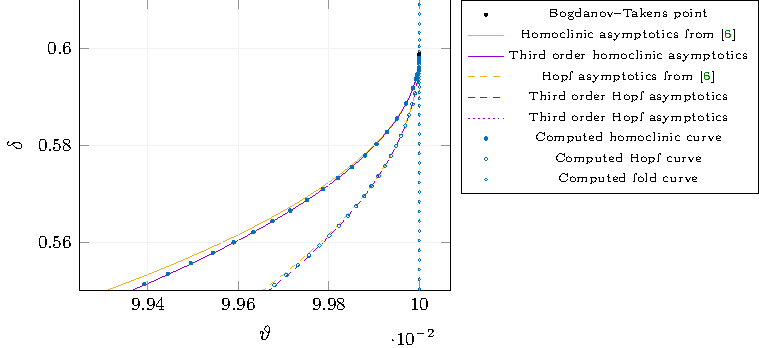
\includegraphics{\imagedir/DoubleAlleeEffectCompareParameters.pdf}
    \caption{Bifurcation diagram near the derived generic Bogdanov-Takens point in
        \cref{btdde:eq:double_alle_effect_rescaled} comparing computed codimension one
        using \DDEBIFTOOL with the asymptotics obtained in this paper and in \cite{Jiao2021}.}
    \label{btdde:fig:DoubleAlleeEffectCompareParameters}
\end{figure}
\begin{figure}[ht!]
    \centering
    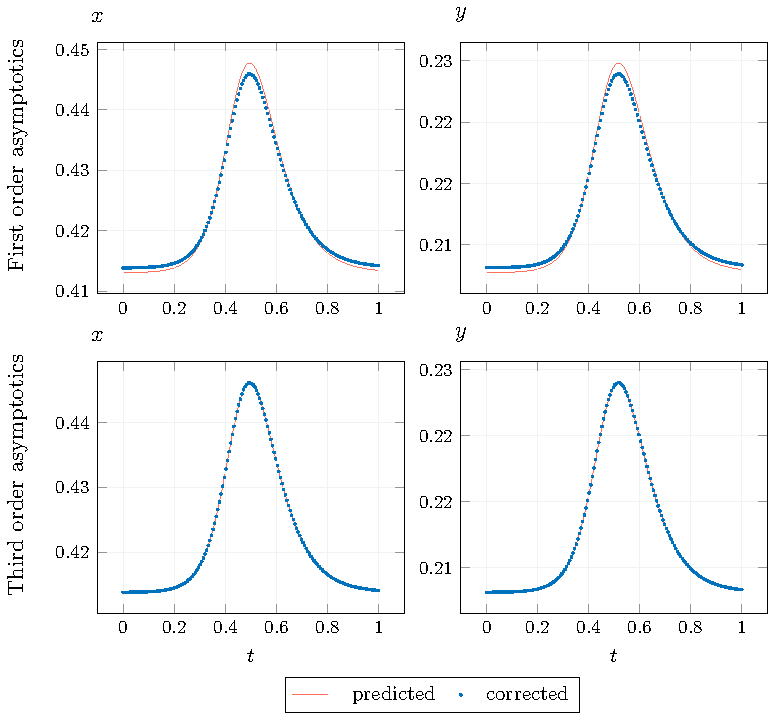
\includegraphics{\imagedir/DoubleAlleeEffectCompareProfiles.pdf}
    \caption{Comparison between the profiles of the first and third-order asymptotics from
    \cref{btdde:sec:generic_bt_homoclinic_asymptotics} with the Newton correct solutions near the generic
        Bogdanov--Takens bifurcation in \cref{btdde:eq:double_alle_effect_rescaled} with the
        perturbation parameter set to $\epsilon=0.3$.}
    \label{btdde:fig:DoubleAlleeEffectCompareProfiles}
\end{figure}
%
\begin{figure}[ht]
    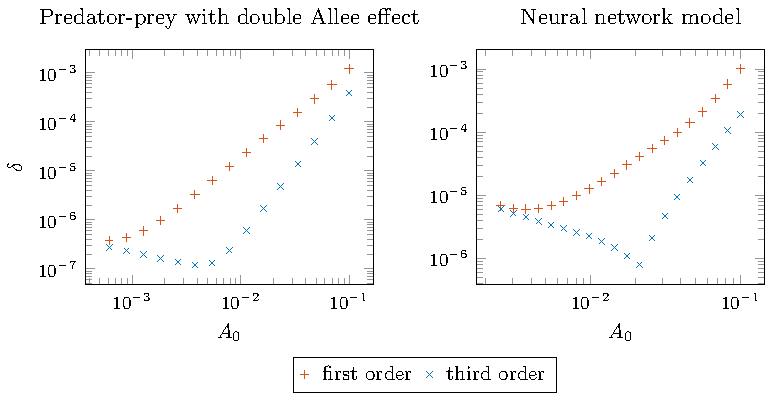
\includegraphics{\imagedir/convergencePlotsGeneric.pdf}
    \caption{On the abscissa is the approximation to the amplitude $A_0$ and on
        the ordinate the relative error $\delta$ between the constructed
        solution to the defining system
        \cite{connecting@2002} for the homoclinic orbit and the Newton
        corrected solution.}
    \label{btdde:fig:convergencePlotsGeneric}
\end{figure}
%
In \cite{Jiao2021} the following predator-prey model with double Allee effect and delay is considered
\begin{equation}
\label{btdde:eq:double_alle_effect}
\begin{cases}
    \dot x(t) = \dfrac{rx}{x+n_0}\left(1-\dfrac1 K\right)\left(x - m_0\right) - \dfrac{cxy}{x+\varrho y},\\
    \dot y(t) = -dy + \dfrac{c_1 x(t-\tau)y}{x(t-\tau) + \varrho y(t-\tau)}.
\end{cases}
\end{equation}
Here, the time delay $\tau \geq 0$ is introduced due to the fact that the
reproduction of predator after consuming the prey is not instantaneous, but is
mediated by some time lag required for gestation.
The variables and parameters occurring in \cref{btdde:eq:double_alle_effect}
have the following meaning:
\begin{itemize}
\item $x,y\colon \mathbb R \rightarrow \mathbb R$ denotes the prey and predator population density, respectively.
\item $r$ denotes the maximum prey population growth in absence of the Allee effect.
\item $K$ is the carrying capacity of the environment.
\item $m_0$ is the Allee threshold.
\item $n_0$ is the auxiliary parameter in order to quantify the strength of the Allee effect.
\item $c$ denotes the capturing rate of the predator.
\item $\varrho$ is the half capturing saturation constant.
\item $c_1$ is the conversion rate of prey into predators biomass.
\item $d$ is the per capita predator mortality rate.
\end{itemize}
Following \cite{Jiao2021}, let $(x,y,t) = \left(K\bar x, \frac K \varrho \bar y, \frac{\bar t}r\right)$, and immediately 
dropping the bars again for readability, then \cref{btdde:eq:double_alle_effect} becomes
\begin{equation}
\label{btdde:eq:double_alle_effect_rescaled}
\begin{cases}
    \dot x(t) = x \left( \dfrac{(1-x)(x-\gamma)}{x+\vartheta} - \dfrac{\alpha y}{x+y} \right), \\
    \dot y(t) = \delta y \left( -1 + \dfrac{ m x(t-\tau) }{ x(t-\tau) + y(t-\tau) }\right),
\end{cases}
\end{equation}
where $\vartheta = \frac{n_0}K, \alpha=\frac c{r\varrho}, \gamma = \frac{m_0}K, \delta = \frac dr$ and $m=\frac{c_1}d$.
In \cite{Jiao2021} the phase-space is (although possible) unnecessarily
enlarged to include a parameter. The resulting extended system is used to
derive conditions for a Bogdanov--Takens bifurcation to occur and obtain the
normal form on the center manifold. In our opinion, one should only use the
extended system to prove the existence of a parameter-dependent center manifold,
from which it then follows that we can perform the normalization method as
described in \cref{btdde:sec:Center_manifold_reduction}. Thus, solving \cref{btdde:eq:double_alle_effect_rescaled}
for a double equilibrium with respect to $(x,y)$ and $\vartheta$ yields
\begin{equation}
    \begin{cases}
        x_0 = \dfrac{m+\alpha-m\alpha+m\gamma}{2m}, \\
        y_0 = (m-1)x_0, \\
        \vartheta_0 = \dfrac{(\alpha+m(1-\alpha+\gamma))^2 - 4m^2\gamma}{4(m-1)m\alpha},
    \end{cases}
\end{equation}
for $m\neq 1$. The parameters should of course be chosen such that $x$ and $y$
are non-negative. The characteristic matrix at
$(x,y,\vartheta)=(x_0,y_0,\vartheta_0)$ becomes
\[
\begingroup
\renewcommand*{\arraystretch}{2.5}
    \Delta(z) = \begin{pmatrix}
        z + \dfrac{1-m}{m^2}\alpha & \dfrac \alpha {m^2} \\
        -\dfrac{(m-1)^2\delta}m e^{-z\tau} & z + \dfrac{(m-1)\delta}m e^{-z\tau},
    \end{pmatrix}
\endgroup
\]
for $m\neq 0$. A simple calculation confirms indeed that $\det\Delta(0)=0$.
Furthermore, $\det\Delta'(0)=\frac{(m-1)(m\delta-\alpha)}{m^2}$ and
$\det\Delta''(0)=2 - \frac{2 (m-1) \delta\tau}{m}$. Thus, for
$(x,y,\vartheta,\delta)=(x_0,y_0,\vartheta_0,\delta_0)$, with $\delta_0 =
\frac\alpha m$, we have a double zero eigenvalue, provided that
$\det\Delta''(0) \neq 0$. To confirm their analytical findings in \cite{Jiao2021}
numerically, the parameters $\gamma=0.15,\alpha=0.9$ and $m=1.50298303$ are
fixed and $(\vartheta,\delta)$ are taken as unfolding parameters. For these
parameters, we indeed have that $\det\Delta''(0) \neq 0$. Calculating the normal
form coefficients $a$ and $b$ reveal that,
\[
a \approx 0.1479, \qquad b \approx 1.4457.
\]
Thus, the codimension two Bogdanov--Takens bifurcation is non-degenerate.
Furthermore, since the equilibrium $(x_0,y_0)$ depends on the unfolding
parameters, we are in the generic case. Using our implementation of the
homoclinic predictor \cref{btdde:sec:generic_bt_homoclinic_asymptotics} in
\DDEBIFTOOL, we start the continuation of the homoclinic branch emanating from
the Bogdanov--Takens point.

In \cref{btdde:fig:DoubleAlleeEffectCompareParameters}, we compare the parameters of
the computed homoclinic branch with our third-order parameter asymptotics and
the parameters for the homoclinic branch given in \cite{Jiao2021}. We observe
that although the derivation of the asymptotics for the parameters is
non-rigorous, it provides a good predictor. Nonetheless, our third-order
asymptotics for the parameter values provides clearly a better approximation to
the parameter values of the computed homoclinic branch.

Of course, most work lies in the derivation of the asymptotics for the
homoclinic solutions in phase-space itself, which is not available in
\cite{Jiao2021}. In  \cref{btdde:fig:DoubleAlleeEffectCompareProfiles} we compare the
first and third-order asymptotics for the profiles of the homoclinic solution.
Here we set the perturbation parameter to $\epsilon=0.3$ such that both
approximations converge and we observe a visual difference.

However, a numerical better way to compare the first and third-order
asymptotics for the homoclinic solution is through the use of a convergence
plots, similarly as in \cite{Bosschaert@Interplay}. In
\cref{btdde:fig:convergencePlotsGeneric} we clearly see an improvement of using the
third-order asymptotics over the first order asymptotics. We furthermore
observe the standard V-shaped graphs due to round-off error.
\begin{figure}[ht]
    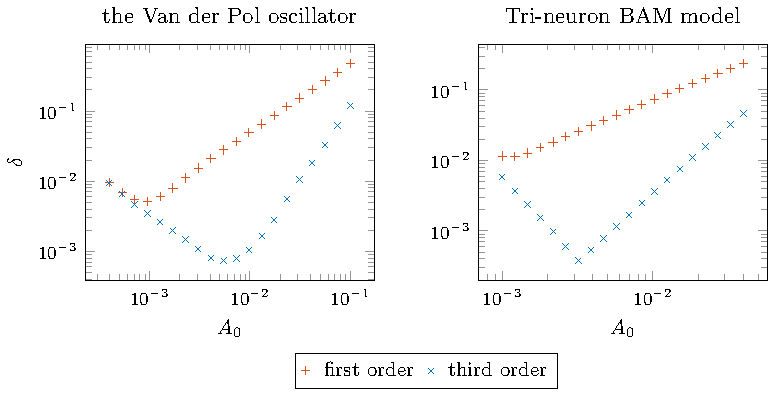
\includegraphics{\imagedir/convergencePlotsTranscritical.pdf}
    \caption{On the abscissa is the approximation to the amplitude $A_0$ and on
        the ordinate the relative error $\delta$ between the constructed solution
        to the defining system for the homoclinic orbit
        and the Newton corrected solution.}
    \label{btdde:fig:convergencePlotsTranscritical}
\end{figure}

\subsection{\ifthesis \phantom{ } \fi Generic Bogdanov--Takens bifurcation in a neural network model}
In this example, we will consider the model 
\begin{equation}
\label{btdde:eq:neural_network}
\begin{cases}
\mu\dot{u}_1(t) = -u_1(t) + q_{11}\alpha(u_1(t - T))-q_{12}u_2(t - T) + e_1,\\
\mu\dot{u}_2(t) = -u_2(t) + q_{21}\alpha(u_1(t - T))-q_{22}u_2(t - T) + e_2,
\end{cases}
\end{equation}
which describes the dynamics of a neural network consisting of an
excitatory and inhibitory neuron \cite{giannakopoulos2001bifurcations}.
The variables and parameters occurring in \cref{btdde:eq:neural_network}
have the following neurophysiological meaning:
\begin{itemize}
\item $u_1,u_2:\mathbb{R}\rightarrow\mathbb{R}$ denote the total post-synaptic
potential of the excitatory and inhibitory neuron, respectively.
\item $\mu>0$ is a time constant characterizing the dynamical properties
of cell membrane.
\item $q_{ik}\geq0$ represents the strength of the connection line from
the $k$th neuron to the $i$th neuron.
\item $\alpha:\mathbb{R}\rightarrow\mathbb{R}$ is the transfer function
which describes the activity generation of the excitatory neuron as
a function of its total potential $u_1$. The function $\alpha$
is smooth, increasing and has a unique turning point at $u_1 = \theta$.
The transfer function corresponding to the inhibitory neuron is assumed
to be the identity.
\item $T\geq0$ is a time delay reflecting synaptic delay, axonal and dendritic
propagation time.
\item $e_1$ and $e_2$ are external stimuli acting on the excitatory
and inhibitory neuron, respectively.
\end{itemize}

Following \cite{giannakopoulos2001bifurcations} we consider the equation \cref{btdde:eq:neural_network} with
\begin{align*}
\alpha(u_1) & = \frac{1}{1 + e^{-4u_1}}-\frac{1}{2},\qquad q_{11} = 2.6,\qquad q_{21} = 1.0,\qquad q_{22} = 0.0,\\
\mu & = 1.0,\qquad T = 1.0,\qquad e_2 = 0.0,
\end{align*}
and $Q: = q_{12},\,E: = e_1$ as bifurcation parameters. Substituting
into \cref{btdde:eq:neural_network} yields
\begin{equation}
\label{btdde:eq:neural_network_subs}
\begin{cases}
\dot{u}_1(t) = -u_1(t) + 2.6\alpha(u_1(t - 1))-Qu_2(t - 1) + E,\\
\dot{u}_2(t) = -u_2(t) + \alpha(u_1(t - 1)).
\end{cases}
\end{equation}
Notice that for any steady-state we have the symmetry
$(u_1,u_2,E)\rightarrow(-u_1,-u_2,-E)$. It is easy to explicitly derive that the system has a double eigenvalue zero for
\begin{equation}
    \left\{
    \begin{aligned}
        u_1(t) &= \frac14 \log\left(\frac{8 - \sqrt{39}}5\right) \approx -0.2617, \\
        u_2(t) &= -\frac12 \sqrt{\frac{3}{13}} \approx -0.2402, \\
        Q &= \frac{13}{10}, \\
        E &= \frac{\sqrt{39} - 10\atanh \sqrt{\frac{3}{13}}}{20} \approx 0.0505.
    \end{aligned}\right.
\end{equation}

The dependence of the equilibria on the parameters $(Q,E)$ yields a generic
Bogdanov--Takens bifurcation, see \cite{giannakopoulos2001bifurcations}. Notice
that the normal form reduction in \cite{giannakopoulos2001bifurcations} is
incorrect, which leads to the normal form for a transcritical Bogdanov--Takens
bifurcation.

\begin{figure}[ht!]
    \centering
    \includetikzscaled{NeuralNetworkCompareParameters}
    \caption{Bifurcation diagram near the derived generic Bogdanov-Takens point in
        \cref{btdde:eq:neural_network_subs} comparing computed codimension one curves using
        \DDEBIFTOOL with the third-order homoclinic parameter asymptotics obtained
        in \cref{btdde:sec:generic_bt_homoclinic_asymptotics}.}
    \label{btdde:fig:NeuralNetworkCompareParameters}
\end{figure}

In \cref{btdde:fig:NeuralNetworkCompareParameters} we compared the computed
codimension one curves emanating from a generic Bogdanov--Takens point in
\cref{btdde:eq:neural_network_subs} using our implementation in \DDEBIFTOOL with the
third-order homoclinic parameter asymptotics obtained in
\cref{btdde:sec:generic_bt_homoclinic_asymptotics}. We see that the predicted and
computed curves are almost indistinguishable. Furthermore, in
\cref{btdde:fig:convergencePlotsGeneric}, we see that using the third-order homoclinic
asymptotics over the first order is clearly superior.

\subsection{Transcritical Bogdanov--Takens bifurcation in the Van der Pol oscillator with delay feedback}
We consider the Van der Pol oscillator with delay feedback \cite{jiang2007bogdanov}
given by 
\begin{equation}
\label{btdde:eq:dde_vanderPol}
\ddot{x}(t) + \epsilon(x^2(t)-1)\dot{x}(t) + x(t) = \epsilon g(x(t-\tau)),
\end{equation}
where $\epsilon>0$ is a parameter, $\tau>0$ is a delay and $g:\mathbb{R}\rightarrow\mathbb{R}$
is a smooth function with $g(0) = 0$ and $g'(0)\neq0$. We rewrite
the Van der Pol equation \cref{btdde:eq:dde_vanderPol} as
\begin{equation}
\label{btdde:eq:vanderPolOscillator}
\begin{cases}
    \dot{x}_1 = x_2,\\
    \dot{x}_2 = \epsilon g(x_1(t-\tau))-\epsilon(x_1^2-1)x_2-x_1.
\end{cases}
\end{equation}
Rescaling time with $t\rightarrow\dfrac{t}{\tau}$ to normalize the
delay yields
\begin{equation}
\label{btdde:eq:vanderPolOscillatorRescaled}
\begin{cases}
\dot{x}_1 = \tau x_2,\\
\dot{x}_2 = \tau\left(\epsilon g(x_1(t-1))-\epsilon(x_1^2-1)x_2-x_1\right).
\end{cases}
\end{equation}
This allows us to treat $\tau$ as a bifurcation parameter.

Following \cite{jiang2007bogdanov}, we consider \cref{btdde:eq:dde_vanderPol} with
\[
g(x) = \frac{e^x-1}{c_1e^x + c_2},
\]
where $c_1 = \dfrac{1}{4}$ and $c_2 = \dfrac{1}{2}$. Then the trivial
equilibrium undergoes a transcritical Bogdanov--Takens bifurcation at parameter
values $(\epsilon,\tau) = (0.75,0.75)$, see \cite{jiang2007bogdanov} and the
supplement. 
%
\begin{figure}[ht]
    \centering
    \includetikzscaled{vanderPolOscillatorCompareParameters}
    \caption{Bifurcation diagram near the derived generic Bogdanov-Takens point in
        \cref{btdde:eq:vanderPolOscillatorRescaled} comparing computed codimension one curves using
        \DDEBIFTOOL with the third-order homoclinic parameter asymptotics obtained
        in \cref{btdde:sec:transcritical_bt_homoclinic_asymptotics}.}
    \label{btdde:fig:vanderPolOscillatorCompareParameters}
\end{figure}

In \cref{btdde:fig:vanderPolOscillatorCompareParameters} we compared the computed
codimension one curves emanating from a transcritical Bogdanov--Takens point in
\cref{btdde:eq:vanderPolOscillatorRescaled} using our implementation in \DDEBIFTOOL
with the third-order homoclinic parameter asymptotics obtained in
\cref{btdde:sec:transcritical_bt_homoclinic_asymptotics}. We see that the predicted
and computed curves are almost indistinguishable. Furthermore, in
\cref{btdde:fig:convergencePlotsTranscritical} we see that using the third-order
homoclinic asymptotics over the first order is clearly superior.

\subsection{Transcritical Bogdanov--Takens bifurcation in a tri-neuron BAM neural network model}
\label{btdde:sec:Tri-neuron-BAM-neural}

We consider a three-component system of a tri-neuron bidirectional
associative memory (BAM) neural network model with multiple delays \cite{dong2013bogdanov}.
The architecture of this BAM model is illustrated in \cref{btdde:fig:BAM_architecture_graph}. 

\begin{figure}
\centering
\includetikzscaled[0.75]{BAM_architecture_graph}
\caption{The graph of architecture for model \cref{btdde:eq:tri_neuron_BAM}.}
\label{btdde:fig:BAM_architecture_graph}
\end{figure}

\begin{figure}[ht]
\centering
\includetikzscaled{triNeuronBAMNeuralNetworkModelCompareParameters}
\caption{
Bifurcation diagram near the transcritical Bogdanov--Takens bifurcation and
a generic Bogdanov--Takens in \cref{btdde:eq:tri_neuron_BAM-u} comparing computed
codimension one using \DDEBIFTOOL with the asymptotics obtained in this
paper.}
\label{btdde:fig:triNeuronBAMNeuralNetworkModelCompareParameters}
\end{figure}

In this model, there is only one neuron with the activation function
$f_{1}$ on the $I$-layer and there are two neurons with respective
activation functions $f_{2}$ and $f_{3}$ on the $J$-layer. It is assumed 
that the time delay from the $I$-layer to the $J$-layer is $\tau_{1}$,
while the time delay from the $J$-layer to the $I$-layer is $\tau_{2}$.
Then the network can be described by the following delay differential equation
\begin{equation}
\label{btdde:eq:tri_neuron_BAM}
\begin{cases}
\dot{x}_{1}(t) & =-\mu_{1}x_{1}(t)+c_{21}f_{1}(x_{2}(t-\tau_{2}))+c_{31}f_{1}(x_{3}(t-\tau_{2})),\\
\dot{x}_{2}(t) & =-\mu_{2}x_{2}(t)+c_{12}f_{2}(x_{1}(t-\tau_{1})),\\
\dot{x}_{3}(t) & =-\mu_{3}x_{3}(t)+c_{13}f_{3}(x_{1}(t-\tau_{1})).
\end{cases}
\end{equation}
Here
\begin{itemize}
\item $x_{i}(t)\,(i=1,2,3)$ denote the state of the neuron at time $t$;
\item $\mu_{i}(i=1,2,3)$ describe the attenuation rate of internal neurons
processing on the $I$-layer and the $J$-layer and $\mu_{i}>0$;
\item the real constants $c_{i1}$and $c_{1i}\,(2,3)$ denote the neurons
in two layers: the $I$-layer and the $J$-layer.
\end{itemize}
Letting $u_{1}(t)=x_{1}(t-\tau_{1}),u_{2}(t)=x_{2}(t),u_{3}(t)=x_{3}(t)$
and $\tau=\tau_{1}+\tau_{2}$, then system \cref{btdde:eq:tri_neuron_BAM}
is equivalent to the following system

\begin{equation}
\label{btdde:eq:tri_neuron_BAM-u}
\begin{cases}
\dot{u}_{1}(t) & =-\mu_{1}u_{1}(t)+c_{21}f_{1}(u_{2}(t-\tau))+c_{31}f_{1}(u_{3}(t-\tau)),\\
\dot{u}_{2}(t) & =-\mu_{2}u_{2}(t)+c_{12}f_{2}(u_{1}(t)),\\
\dot{u}_{3}(t) & =-\mu_{3}u_{3}(t)+c_{13}f_{3}(u_{1}(t)).
\end{cases}
\end{equation}

In \cite{dong2013bogdanov} conditions for \cref{btdde:eq:tri_neuron_BAM-u} are derived
for the origin to have a double zero eigenvalue, while all other eigenvalues
have negative real parts. Since the provided expression did not give the correct results,
we corrected the given expression from \cite{dong2013bogdanov}.
We postpone the proof of the next two lemma's to the 
\ifthesis%
    \cref{chapter:BT_DDE_supplement}%
\fi%
\ifsiam%
    \hyperref[mysupplement]{online Supplement}%
\fi%
\ifarxiv%
    \hyperlink{mysupplement}{Supplement}%
\fi.

\begin{lemma}
\label{btdde:lem:BAM_double_eigenvalue}
Assume that $f_{i}(0)=0\,(i=1,2,3)$,
$f_{i}'(0)\neq0\,(i=1,2,3)$ and $\mu_{2}\neq\mu_{3}$, then the steady-state
$(u_{1},u_{2},u_{3})=(0,0,0)$ has a double zero eigenvalue at 
\begin{align*}
c_{21} & =c_{21}^{0}=\frac{\mu_{2}^{2}\left(\mu_{1}\left(\mu_{3}\tau+1\right)+\mu_{3}\right)}{c_{12}\left(\mu_{2}-\mu_{3}\right)f_{1}'(0)f_{2}'(0)},\\
c_{31} & =c_{31}^{0}=\frac{\mu_{3}^{2}\left(\mu_{1}\left(\mu_{2}\tau+1\right)+\mu_{2}\right)}{c_{13}\left(\mu_{3}-\mu_{2}\right)f_{1}'(0)f_{3}'(0)}.
\end{align*}
\end{lemma}

\begin{lemma}
\label{btdde:lemma:triNeuralBAMNetworkModelEigenvalues}
\textup{Correction to \cite[Lemma 3]{dong2013bogdanov}.}
Let $(c_{21},c_{31})=(c_{21}^{0},c_{31}^{0})$,
\begin{equation}
    \label{btdde:sm:eq:omega_0} 
    \omega_0 = \frac{\sqrt{-\mu_1^2 - \mu_2^2 - \mu_3^2 + \sqrt{\zeta_0}}}{\sqrt{2}}
\end{equation}
and $0<\tau<\tau_{0}$, where $\tau_0$ is the minimum positive solution to the nonlinear equation
\begin{equation}
    \label{btdde:sm:eq:tan} 
    \tan (\tau \omega_0) = \frac{b_0\zeta_1 - a_0\zeta_2}{a_0\zeta_1 + b_0\zeta_2},
\end{equation}
with
\begin{align*}
a_0 &= -\mu_1\mu_2\mu_3, \\ 
b_0 &= -\omega_0(\mu_2\mu_3 + \mu_1(\mu_2 + \mu_3 + \mu_2\mu_3\tau)), \\
\zeta_0 &= \mu_1^4 + (\mu_2^2 + \mu_3^2)^2 + 8\mu_1\mu_2\mu_3(\mu_2 + \mu_3 + \mu_2\mu_3\tau) + \\
        &\qquad 2\mu_1^2(\mu_3^2 + 4\mu_2\mu_3(1 + \mu_3\tau) + \mu_2^2(1 + 2\mu_3\tau(2 + \mu_3\tau))), \\
\zeta_1 &= \mu_1\mu_2\mu_3 - (\mu_1 + \mu_2 + \mu_3)\omega_0^2, \\
\zeta_2 &= \mu_2\mu_3\omega_0 + \mu_1(\mu_2 + \mu_3)\omega_0 - \omega_0^3.
\end{align*}
Then the center manifold near the Bogdanov--Takens point is locally attractive.
\end{lemma}

For the numerical verification we consider, as in the simulations in
\cite[Example 1]{dong2013bogdanov}, the system \cref{btdde:eq:tri_neuron_BAM-u} with
the activation functions
\[
f_{1}(x)=\tanh(x)+0.1x^{2},\quad f_{2}(x)=f_{3}(x)=\tanh(x),
\]
and parameter values
\[
\mu_{1}=0.1,\mu_{2}=0.3,\mu_{3}=0.2,c_{12}=c_{13}=1,\tau=5.
\]
Then, from \cref{btdde:lem:BAM_double_eigenvalue}, we obtain two critical
values 
\[
(c_{21}^{0},c_{31}^{0})=(0.36,-0.22),
\]
at which there is a transcritical Bogdanov--Takens point. Furthermore, since
$\tau < \tau_0 \approx 5.4320$ the center manifold is attractive. In fact, we
will show in the
\ifthesis%
    \cref{chapter:BT_DDE_supplement} %
\fi%
\ifsiam%
    \hyperref[mysupplement]{online Supplement} %
\fi%
\ifarxiv%
    \hyperlink{mysupplement}{Supplement} %
\fi
that the center manifold is attractive for
$0<\tau<13.2309348879375$. We write the system \cref{btdde:eq:tri_neuron_BAM-u}
as
\begin{equation}
\label{btdde:eq:tri_neuron_BAM-u-1}
\begin{cases}
\dot{u}_{1}(t) & =-\mu_{1}u_{1}(t)+\left(c_{21}^{0}+\alpha_{1}\right)f_{1}(u_{2}(t-\tau))+\left(c_{31}^{0}+\alpha_{2}\right)f_{1}(u_{3}(t-\tau)),\\
\dot{u}_{2}(t) & =-\mu_{2}u_{2}(t)+c_{12}f_{2}(u_{1}(t)),\\
\dot{u}_{3}(t) & =-\mu_{3}u_{3}(t)+c_{13}f_{3}(u_{1}(t)),
\end{cases}
\end{equation}
where $(\alpha_{1},\alpha_{2})$ are the new parameter values such
that at $(\alpha_{1},\alpha_{2})=(0,0)$ we have a Bogdanov-Takens
bifurcation. The critical normal form coefficients 
\[
(a,b)\approx(0.0012,-0.0135),
\]
indicate stable cycles. In
\cref{btdde:fig:triNeuronBAMNeuralNetworkModelCompareParameters}, we have plotted the
local unfolding of the transcritical Bogdanov-Takens bifurcation using our
implementation in DDE-BifTool to start the continuation of the transcritical,
Hopf, and homoclinic codimension one bifurcation curves. Furthermore, using the
ability to detect codimension two bifurcation points while continuing Hopf
points, we discovered another Bogdanov--Takens point. From the transversality
conditions, we see the secondary Bogdanov--Takens point is of the generic case.
Thus, we can start continuation of the homoclinic orbits emanating from this
point as well. We see that the numerically continued homoclinic curves in the
upper half plane only exists in a very small parameter region. Without our
predictor, this homoclinic curve would be extremely difficult to locate. Lastly,
in \cref{btdde:fig:convergencePlotsTranscritical} the first and third-order
homoclinic asymptotics are compared. Here we again see expected improvements of using the
third-order homoclinic asymptotics. We refer to the
\ifthesis%
    \cref{chapter:BT_DDE_supplement} %
\fi%
\ifsiam%
    \hyperref[mysupplement]{online Supplement} %
\fi%
\ifarxiv%
    \hyperlink{mysupplement}{Supplement} %
\fi to see the beautiful
homoclinic orbits along the homoclinic curve in the lower half plane, and for
an overall more detailed treatment of this example. In fact, we will show that
the transcritical Bogdanov--Takens and generic Bogdanov--Takens points are
connected, not only by a Hopf curve, but also through a homoclinic curve. 

\section{Concluding remarks}
We have provided explicit formulas needed to initialize the codimension one
equilibrium and homoclinic bifurcations emanating from the transcritical and
generalized codimension two Bogdanov--Takens bifurcation point in classical
DDEs. Applications to four different models are given, confirming the
correctness of the derivation of the time-reparametrization
parameter-dependent
center manifold transformation and the codimension one asymptotics.

By extending the normalization technique to include a time-reparametrization we
are allowed to use orbital normal forms, instead of only smooth normal forms.
One benefit of this approach is the reusability of the codimension one curves
emanating from the universal unfolding of the Bogdanov--Takens codimension two
bifurcation. Indeed, by a simple transformation \cref{btdde:eq:blowup}, we obtain the
homoclinic asymptotics for the transcritical Bogdanov--Takens bifurcation.

In this paper, we have restricted to the class of classical DDEs, and for the
applications to the class of discrete DDEs. However, the proof in
\cite{Switching2019} of the existence of a smooth parameter-dependent center
manifold is given in the general context of perturbation theory for dual
semigroups (sun-star calculus). Therefore, the applicability of this result
extends beyond classical DDEs. For example, in \cite{VanGils2013} and
\cite{Dijkstra2015} the technique was used to calculate the critical normal
form coefficients for Hopf and Hopf-Hopf bifurcations occurring in neural field
models with propagation delays. For these models, sun-reflexivity is lost, which
is typical for delay equations in abstract spaces or with infinite delay.
However, it is often possible to overcome this functional analytic
complication, so dual perturbation theory can still be employed successfully
\cite{Diekmann2008,Diekmann2012blending,VanGils2013,Janssens2019}. It follows
that the derived coefficients in
\cref{btdde:sec:parameter-dependent-center-manifold-reduction} are valid in these
settings as well.

Similarly, in \cite{Sieber@2017} it is demonstrated that formally the
normalization method still works for state-dependent delay differential
equations. However, for our formulas to work in this situation, one first needs
to implement the continuation of homoclinic orbits for state-dependent DDEs. Of
course, the asymptotics are still useful to see where     the homoclinic orbit
should be located. Furthermore, the asymptotics can be used to numerically
approximate the homoclinic solutions by periodic orbits with a large return
time.

Returning to the setting of classical DDEs, the most obvious next challenge is
to derive normal forms for bifurcations of periodic orbits by generalizing
\cite{Kuznetsov2005,DeWitte2013,DeWitte2014}. The resulting formulas can then
be implemented in \DDEBIFTOOL to facilitate numerical bifurcation analysis of
periodic orbits in supported types of classical DDEs.


%% DDE BT Supplement 
\chapter[Supplementary materials]
        {Supplementary materials to Bifurcation analysis of Bogdanov-Takens bifurcations in delay differential equations}
\label{chapter:BT_DDE_supplement}
\paragraph{{\color{header1}Abstract}}In this supplement, we will provide a full walk-through of the examples given
in \cref{btdde:sec:Examples} with
\DDEBIFTOOL\footnote{\url{http://ddebiftool.sourceforge.net/}}
\cite{2014arXiv1406.7144S}. Additionally, the Julia code, used for the
numerical simulation, with the package {\tt
DifferentialEquations.jl}\footnote{\url{https://github.com/SciML/DifferentialEquations.jl}}
\cite{rackauckas2017differentialequations} is shown. Some new results were
obtained while studying these models.

This allows other researchers to fully replicate the findings in the main text.
Other DDE models, undergoing generic or transcritical Bogdanov--Takens
bifurcations treated in this paper, can easily be studied by simply modifying
the given code. The code here has also been included into the \DDEBIFTOOL
package on the source-forge repository and can be executed without the need to
copy and paste. In this supplement we mainly focus on the initialization and
continuation of the various codim-1 equilibrium and homoclinic bifurcation
curves emanating from the Bogdanov--Takens points and also on numerical
simulation near the bifurcation points. For a more complete overview of the
capabilities and functionality for \DDEBIFTOOL we refer to the online tutorials
files and also the manual and the references therein.

Note that reading this supplement may feel at times somewhat repetitive. We see
this as a positive sign. Indeed, our predictors need little adjustment
before starting continuation of the codimension one curves emanating from the
generic and transcritical Bogdanov--Takens bifurcation.

To follow the examples below, we recommend using the \DDEBIFTOOL package
supplied with the article. Also note that the \MATLAB code has been tested on 
\MATLAB 2020b and \OCTAVE 6.4.0 using \OCTAVE symbolic
package version 2.9.0. Different results may occur on other version of 
\MATLAB or \OCTAVE.


\section[Predator-prey system with double Allee effect]
        {Generic Bogdanov--Takens bifurcation in a Predator-prey system with double Allee effect}
In \cite{Jiao2021} the following predator-prey model with double Allee effect
and delay is considered
\begin{equation}
\label{sm:eq:double_alle_effect}
\begin{cases}
    \dot x(t) = \dfrac{rx}{x+n_0}\left(1-\dfrac1 K\right)\left(x - m_0\right) - \dfrac{cxy}{x+\varrho y},\\
    \dot y(t) = -dy + \dfrac{c_1 x(t-\tau)y}{x(t-\tau) + \varrho y(t-\tau)}.
\end{cases}
\end{equation}
Here the time delay $\tau \geq 0$ is introduced due to the fact that the
reproduction of predator after consuming the prey is not instantaneous, but is
mediated by some time lag required for gestation.
The variables and parameters occurring in \cref{sm:eq:double_alle_effect}
have the following meaning:
\begin{itemize}
\item $x,y\colon \mathbb R \rightarrow \mathbb R$ denotes the prey and predator population density, respectively.
\item $r$ denotes the maximum prey population growth in absence of the Allee effect.
\item $K$ is the carrying capacity of the environment.
\item $m_0$ is the Allee threshold.
\item $n_0$ is the auxiliary parameter in order to quantify the strength of the Allee effect.
\item $c$ denotes the capturing rate of the predator.
\item $\varrho$ is the half capturing saturation constant.
\item $c_1$ is the conversion rate of prey into predators biomass.
\item $d$ is the per capita predator mortality rate.
\end{itemize}
Following \cite{Jiao2021} let $(x,y,t) = \left(K\bar x, \frac K \varrho \bar y, \frac{\bar t}r\right)$, and immediately 
dropping the bars again for readability, then \cref{sm:eq:double_alle_effect} becomes
\begin{equation}
\label{sm:eq:double_alle_effect_rescaled}
\begin{cases}
    \dot x(t) = x \left( \dfrac{(1-x)(x-\gamma)}{x+\vartheta} - \dfrac{\alpha y}{x+y} \right), \\
    \dot y(t) = \delta y \left( -1 + \dfrac{ m x(t-\tau) }{ x(t-\tau) + y(t-\tau) }\right),
\end{cases}
\end{equation}
where $\vartheta = \frac{n_0}K, \alpha=\frac c{r\varrho}, \gamma = \frac{m_0}K, \delta = \frac dr$ and $m=\frac{c_1}d$.


Thus, $(x,y,\vartheta,\delta)=(x_0,y_0,\vartheta_0,\delta_0)$, with $\delta_0 =
\frac\alpha m$, we have a double zero eigenvalue, provided that
$\det\Delta''(0) \neq 0$. To confirm their analytical findings in \cite{Jiao2021}
numerically, the parameters $\gamma=0.15,\alpha=0.9$ and $m=1.50298303$ are
fixed and $(\vartheta,\delta)$ are taken as unfolding parameters. For these
parameters, we indeed have that $\det\Delta''(0) \neq 0$.

\begin{remark}
    The \MATLAB files for this demonstration can be found in the directory
    \mintinline[breaklines,breakafter=/]{MATLAB}{demos/tutorial/VII/neural_network_model} relative to the main
    directory of the \DDEBIFTOOL package.
\end{remark}

\subsection{Generate system files}
Before we start to analyze the system with \DDEBIFTOOL, we first create a
\emph{system file}. This file contains the definition of the system
\cref{sm:eq:double_alle_effect_rescaled}, the standard derivatives needed for
calculation of the eigenvalues and eigenvectors, the continuation of
bifurcation points cycles, and also the multilinear forms, see \cite[Section
6]{Switching2019}, used for the calculation of the coefficients of the critical
and parameter-dependent normal forms and center manifold transformation.
Alternatively, one can only supply the system itself, see
\cref{sm:lst:wo_system_file}. Then finite difference is used to approximate the
derivatives. However, this is less efficient and accurate, and therefore not
recommended. A separate script \mintinline{MATLAB}{gen_sym_predator_prey.m} is used to
create a system file. The most important parts of this script are listed and
discussed below.

%% Add paths and load sym package if GNU Octave is used
\newcommand\pathToDDEBifToolDemos{/home/maikel/Documents/MySoftware/ddebiftool-git/demos/tutorials/VII}
\inputminted[firstline=18, lastline=50]{MATLAB}{\pathToDDEBifToolDemos/predator_prey/gen_sym_predator_prey.m}
The variable \mintinline{MATLAB}{ddebiftoolpath} is directed to the \DDEBIFTOOL main
folder, which should have been extracted somewhere on the computer. Here, a path
relative to the current working directory is used. Note that although we only
use the parameters $(\theta,\delta)$ as unfolding parameters, in the current
version of \DDEBIFTOOL, we also need to include the delay(s) in the list of
parameters. After running the script, the function \mintinline{MATLAB}{dde_sym2funcs}
creates two system files \mintinline{MATLAB}{sym_predator_prey_mf.m} and \mintinline{MATLAB}{sym_predator_prey.m}.
The first file \mintinline{MATLAB}{sym_predator_prey_mf.m} implements the higher order derivatives
as multilinear forms, as explained in \cite[Section 6]{Switching2019}, and therefore the
file we will solely be using. The second file \mintinline{MATLAB}{sym_predator_prey.m}
uses directional derivatives to implement the higher order derivatives. The
directional derivatives approach \emph{formally} allows the use of
state-dependent delays, see \cite{Sieber@2017}. Although both approaches yields
(up to rounding errors) identical normal form coefficients and center manifold
transformations, multilinear forms are more efficient.

\subsection{Loading the \DDEBIFTOOL package}
\label{sm:sec:loading_DDE-BIFTool}
Now that a system file is created we continue with \DDEBIFTOOL to analyze
\cref{sm:eq:double_alle_effect_rescaled} numerically. The code in the following
sections highlights the import parts of the file \mintinline{MATLAB}{predator_prey.m}.
\DDEBIFTOOL consists of a set of \MATLAB routines. Thus, in order to start
using \DDEBIFTOOL, we only need to add \DDEBIFTOOL directories to the search
path.
\begin{listing}[H]
\inputminted[firstline=17, lastline=25]{MATLAB}{\pathToDDEBifToolDemos/predator_prey/predator_prey.m}
\caption{Code to add \DDEBIFTOOL scripts to the search path.}
\label{sm:lst:searchpath}
\end{listing}
There are four subdirectories added to the search path:
\par
\medskip
\begin{description}
\item[ddebiftool] Containing the core files of \DDEBIFTOOL.
\item[ddebiftool\_extra\_psol] An extension for enabling continuation of periodic orbit bifurcations for delay-differential equations with constant or state-dependent delay.
\item[ddebiftool\_extra\_nmfm] An extension for normal form computation.
\item[ddebiftool\_utilities] Containing various utilities.
\end{description}

\subsection{Set parameter names}
The following code allows us to use
\mintinline{MATLAB}{ind.theta} instead of remembering the
index of the parameter $\beta$ in the parameter array, and similarly for the
other parameters.
\inputminted[firstline=27, lastline=30]{MATLAB}{\pathToDDEBifToolDemos/predator_prey/predator_prey.m}
In this way, fewer mistakes are likely to be made, and the code is easier to read.

\subsection{Initialization}
Next, we set up the \mintinline{MATLAB}{funcs} structure, containing information about
where the system and its derivatives are stored, a function pointing to which
parameters are delays, and various other settings.
\inputminted[firstline=32, lastline=35]{MATLAB}{\pathToDDEBifToolDemos/predator_prey/predator_prey.m}
Alternatively, when no system files have been generated, one could initialize
the system \cref{sm:eq:double_alle_effect_rescaled} as follows.

\begin{listing}[H]
\begin{minted}{MATLAB}
%% Define funcs structure without symbolic derivatives
m = 1.502983803;
alpha = 0.9;
gamma = 0.15;
dx_dt = @(x,y,theta) x.*((1-x).*(x-gamma)./(x+theta) ...
                     - alpha.*y./(x+y))
dy_dt = @(y,xt,yt,delta) delta.*y.*(-1 + m.*xt./(xt+yt))
predator_prey_sys = @(xx,par)  ...
   [dx_dt(xx(1,1,:),xx(2,1,:),par(1,ind.theta,:)); ...
    dy_dt(xx(2,1,:),xx(1,2,:),xx(2,2,:),par(1,ind.delta,:))];
% % Set funcs structure
funcs = set_funcs('sys_rhs', predator_prey_sys, ...
    'sys_tau', @() ind.tau,...
    'x_vectorized', true, 'p_vectorized', true);
\end{minted}
\caption{Code to define the system without a system file.}
\label{sm:lst:wo_system_file}
\end{listing}
Inspecting the output of the \mintinline{MATLAB}{funcs} handle gives.
\begin{minted}{shell-session}
>> funcs

funcs =

  struct with fields:

                 sys_rhs: @(x,p)dde_wrap_rhs(x,p,funcs.sys_rhs,funcs.x_vectorized,
                            funcs.p_vectorized)
                sys_ntau: @()0
                 sys_tau: @()ind.tau
                sys_cond: @dde_dummy_cond
                sys_deri: @(x,p,nx,np,v)dde_gen_deriv(funcs.sys_dirderi,x,p,nx,np,v,1)
                sys_dtau: []
              sys_mfderi: {}
             sys_dirderi: {@(x,p,dx,dp)dde_dirderiv(derivbase,x,p,dx,dp,
                            order-ldirderi, 'nf',size(x,1),'hjac',
                            funcs.hjac(order))  [function_handle]}
             sys_dirdtau: []
            x_vectorized: 1
            p_vectorized: 1
                    hjac: @(ord)eps^(1/(2+ord))
      sys_cond_reference: 0
              lhs_matrix: @(sz)lhs_matrix(sz,funcs.lhs_matrix)
                  tp_del: 0
       sys_deri_provided: 0
    sys_dirderi_provided: 0
\end{minted}
The output shows that no derivative file is supplied. In this case, the
derivatives are calculated using finite-difference approximations with the
function \mintinline{MATLAB}{dde_dirderiv}. Again, we do not recommend using the latter
approach. However, it can be useful for debugging purposes.

\subsection{Set parameter range}
Since we are only interested here in the local unfolding we restrict the
allowed parameter range for the unfolding parameters. In practice one may have
physical restrictions which must be satisfied. Additionally, we also limit the
maximum allowed step size during continuation. By doing so we obtain more refined
data to compare against our predictors.
\inputminted[firstline=37, lastline=40]{MATLAB}{\pathToDDEBifToolDemos/predator_prey/predator_prey.m}

\subsection{Stability and coefficients of the generic Bogdanov--Takens point}
We manually construct a steady-state at the Bogdanov--Takens point derived in
\cref{btdde:sec:example:predator_prey}, see also \cite{Jiao2021}.
\inputminted[firstline=42, lastline=55]{MATLAB}{\pathToDDEBifToolDemos/predator_prey/predator_prey.m}
Inspecting the \mintinline{MATLAB}{stst.stability} structure yields
\begin{minted}{shell-session}
>> stst.stability.l1

ans =

   1.0e-06 *

   0.197590320692559
  -0.197590756777676

>> 
\end{minted}

The eigenvalues confirm that the point under consideration is indeed (an
approximation to) a Bogdanov--Takens point. Next, we convert the steady-state
point to a Bogdanov--Takens point and calculate the normal form coefficients
with the function \mintinline{MATLAB}{nmfm_bt}, which implements the coefficients
derived in \cref{btdde:sec:generic_bogdanov-takens}. For this we need to set the argument
\inputminted[firstline=57, lastline=60]{MATLAB}{\pathToDDEBifToolDemos/predator_prey/predator_prey.m}
The coefficients for the normal form, the time-reparametrization, and the center
manifold transformation coefficients are stored in the \mintinline{MATLAB}{bt.nmfm}
structure. Additionally, also the approximation to the parameters and center
manifold transformation is given, which is used for the predictors.
\begin{minted}{shell-session}
>> bt.nmfm

ans =

  struct with fields:

          a: -0.145177185481861
          b: -1.446000370122628
  theta1000: -0.200700969579673
  theta0001: 5.128950206684711
        K10: [2x1 double]
        K01: [2x1 double]
        K02: [2x1 double]
        K11: [2x1 double]
        K03: [2x1 double]
       phi0: [1x1 struct]
       phi1: [1x1 struct]
      h0010: [1x1 struct]
      h0001: [1x1 struct]
      h2000: [1x1 struct]
      h1100: [1x1 struct]
      h0200: [1x1 struct]
      h1010: [1x1 struct]
      h1001: [1x1 struct]
      h0110: [1x1 struct]
      h0101: [1x1 struct]
      h0002: [1x1 struct]
      h0011: [1x1 struct]
      h3000: [1x1 struct]
      h2100: [1x1 struct]
      h1101: [1x1 struct]
      h2001: [1x1 struct]
      h0003: [1x1 struct]
      h1002: [1x1 struct]
      h0102: [1x1 struct]
          K: @(beta1,beta2)K10*beta1+K01*beta2+1/2*K02*beta2.^2
                +K11*beta1.*beta2+1/6*K03*beta2^3
          H: [function_handle]
\end{minted}

Since the sign of $ab$ is positive we expect to find unstable periodic orbits nearby the 
Bogdanov--Takens point.

\subsection{Comparing profiles of computed and predicted homoclinic orbits}
To test the homoclinic asymptotics from
\cref{btdde:sec:generic_bt_homoclinic_asymptotics} we compare the first and third
order asymptotics to the Newton corrected solution. For this we use the 
function \mintinline[breaklines,breakafter=_]{MATLAB}{C1branch_from_C2point}. This function returns a branch, which
by default returns two initial corrected approximations in order to start continuation of the
codimension one curve under consideration. By setting the argument
\mintinline{MATLAB}{'predictor'} to \mintinline{MATLAB}{true} the approximations are left uncorrected.
To make the comparison visually clear we set the perturbation parameter 
$\epsilon=0.3$ (\mintinline{MATLAB}{step = 0.3} in the code below).
The code below produces \cref{sm:fig:DoubleAlleeEffectCompareProfiles}.
The difference between the two approximations is clearly noticeable. While
the first order asymptotics is close to the Newton corrected solution, the third
order asymptotics is indistinguishable at this scale from the Newton corrected
solution.
\inputminted[firstline=62, lastline=80]{MATLAB}{\pathToDDEBifToolDemos/predator_prey/predator_prey.m}
\begin{figure}[ht]
    \centering
    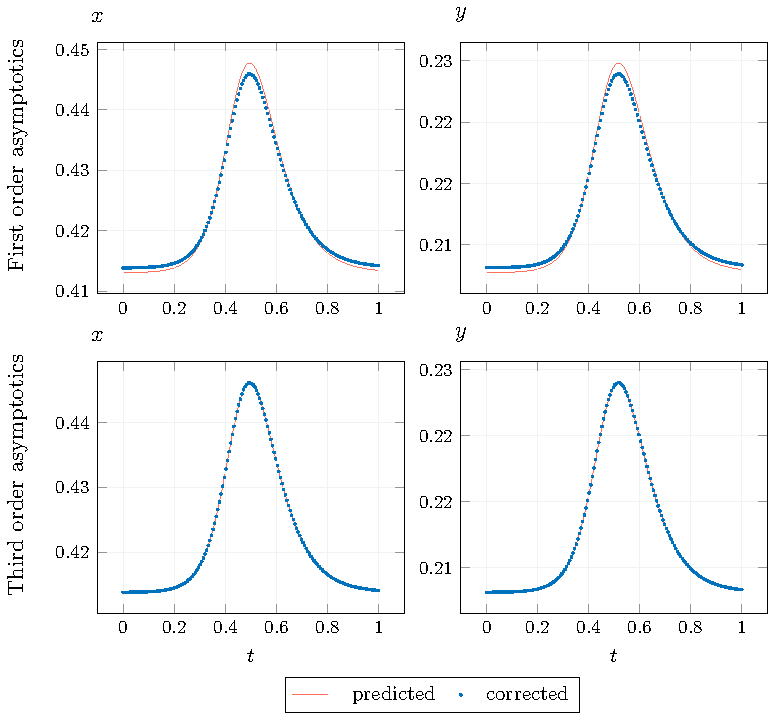
\includegraphics{\imagedir/DoubleAlleeEffectCompareProfiles.pdf}
    \caption{Comparison between the first and third-order asymptotics from
    \cref{btdde:sec:generic_bt_homoclinic_asymptotics} near the generic
        Bogdanov--Takens bifurcation in \cref{sm:eq:double_alle_effect_rescaled} with the
        perturbation parameter set to $\epsilon=0.3$.}
    \label{sm:fig:DoubleAlleeEffectCompareProfiles}
\end{figure}

\subsection{Continuation of the codimension one curves emanating}
To continue the three codimension one curves emanating from the generic
Bogdanov--Takens we can simply use the function
\mintinline[breaklines,breakafter=_]{MATLAB}{C1branch_from_C2point}, as show in the code below. To monitor the
continuation process the argument \mintinline{MATLAB}{plot} must be set \mintinline{MATLAB}{1}.
The most important setting is the perturbation parameter (or multiple),
\mintinline{MATLAB}{step} in the code below. If left out, default stepsizes are defined.
However, depending on the problem no convergence may then be obtained.
\inputminted[firstline=82, lastline=100]{MATLAB}{\pathToDDEBifToolDemos/predator_prey/predator_prey.m}

\subsection{Predictors of the codimension one curves emanating from the Bogdanov--Takens point}
Before we provide the bifurcation diagram in the next section we first obtain
the predictors for the codimension one curves. For this we again use the
function \mintinline[breaklines,breakafter=_]{MATLAB}{C1branch_from_C2point}. We set the argument
\mintinline{MATLAB}{predictor} to \mintinline{MATLAB}{1} and provide a range of
perturbation parameters.
\inputminted[firstline=118, lastline=137]{MATLAB}{\pathToDDEBifToolDemos/predator_prey/predator_prey.m}
In the last part of the code above we added the asymptotics obtained from \cite{Jiao2021}.

\subsection{Bifurcation diagram}
The code below produces a similar figure as \cref{sm:fig:DoubleAlleeEffectCompareParameters} in \MATLAB.
%% Plot the bifurcation curves with predictors
\inputminted[firstline=139, lastline=164]{MATLAB}{\pathToDDEBifToolDemos/predator_prey/predator_prey.m}
%
\begin{figure}[ht]
    \centering
    % this file is generated as a standalone document, to include the reference
    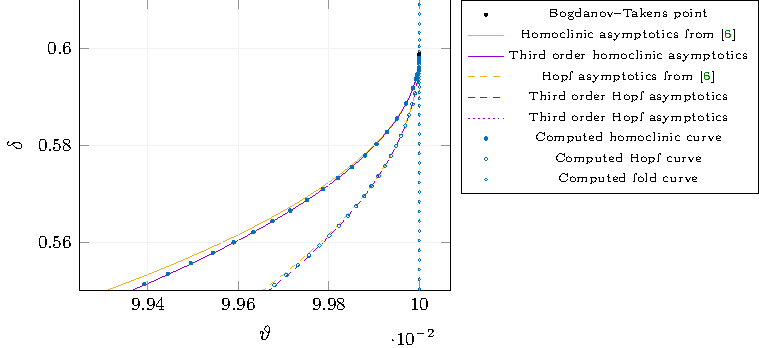
\includegraphics{\imagedir/DoubleAlleeEffectCompareParameters.pdf}
    \caption{Bifurcation diagram near the analytically derived generic Bogdanov-Takens point in
        \cref{sm:eq:double_alle_effect_rescaled} comparing computed codimension one
        curves using \DDEBIFTOOL with the asymptotics obtained in this paper and in \cite{Jiao2021}.}
    \label{sm:fig:DoubleAlleeEffectCompareParameters}
\end{figure}

\subsection{Compare homoclinic solutions in phase-space}
To obtain an impression of the third-order homoclinic asymptotics in
phase-space, we compare the correct and uncorrected homoclinic solution
with the perturbation parameter ranging from $0.1$ to $0.3$.
The code below results in \cref{sm:fig:DoubleAlleeEffectCompareOrbitsPhaseSpace}.
We see that the corrected and predicted homoclinic orbits are nearly identical.
\inputminted[firstline=166, lastline=182]{MATLAB}{\pathToDDEBifToolDemos/predator_prey/predator_prey.m}
The \MATLAB console shows the following output.
\begin{minted}{shell-session}
hcli from BT: branch 1 of  1 correction of point 1, success=1
hcli from BT: branch 1 of  1 correction of point 2, success=1
hcli from BT: branch 1 of  1 correction of point 3, success=1
hcli from BT: branch 1 of  1 correction of point 4, success=1
hcli from BT: branch 1 of  1 correction of point 5, success=1
hcli from BT: branch 1 of  1 correction of point 6, success=1
hcli from BT: branch 1 of  1 correction of point 7, success=1
hcli from BT: branch 1 of  1 correction of point 8, success=1
hcli from BT: branch 1 of  1 correction of point 9, success=1
hcli from BT: branch 1 of  1 correction of point 10, success=1
\end{minted}
That is, all predictions in this range are successfully corrected.
%
\begin{figure}[ht]
    \centering
    \includetikzscaled{DoubleAlleeEffectCompareOrbitsPhaseSpace}
    \caption{Plot comparing the third-order homoclinic asymptotics from
    \cref{btdde:sec:generic_bt_homoclinic_asymptotics} near the generic
    Bogdanov--Takens bifurcation in \cref{sm:eq:double_alle_effect_rescaled} with
    the Newton correct homoclinic solutions in $(x,y)$ phase-space.}
    \label{sm:fig:DoubleAlleeEffectCompareOrbitsPhaseSpace}
\end{figure}

\subsection{Convergence plot}
In \cref{sm:fig:DoubleAlleeEffectCompareProfiles} we compared the profiles of
the first and third-order homoclinic asymptotics. Although the improvement of
the third-order asymptotics is clearly visible, a better way to numerically
compare the different orders is by creating a log-log convergence plot. 
Since we create convergence plots for all examples treated in this supplement,
we created the function \mintinline{MATLAB}{convergence_plot}.
\begin{code}
\inputminted{MATLAB}{\pathToDDEBifToolDemos/convergence_plot.m}
\label{sm:lst:convergence_plot}
\caption{Auxiliary function for creating convergence plots.}
\end{code}
Using this function, the code below yields \cref{sm:fig:DoubleAlleeEffectConvergencePlot}.
%% Convergence plot
\inputminted[firstline=184, lastline=195]{MATLAB}{\pathToDDEBifToolDemos/predator_prey/predator_prey.m}
%
\begin{figure}[ht]
    \centering
    \includetikz{DoubleAlleeEffectConvergencePlot}
    \caption{On the abscissa is the approximation to the amplitude $A_0$ and on the ordinate the
        relative error $\delta$ between the constructed solution
        \mintinline{MATLAB}{hcli_pred} to the defining system for the homoclinic orbit and
        the Newton corrected solution \mintinline{MATLAB}{hcli_corrected}.}
    \label{sm:fig:DoubleAlleeEffectConvergencePlot}
\end{figure}



\subsection{Simulation with {\tt DifferentialEquations.jl}}
%
\begin{figure}[ht!]
    \centering
    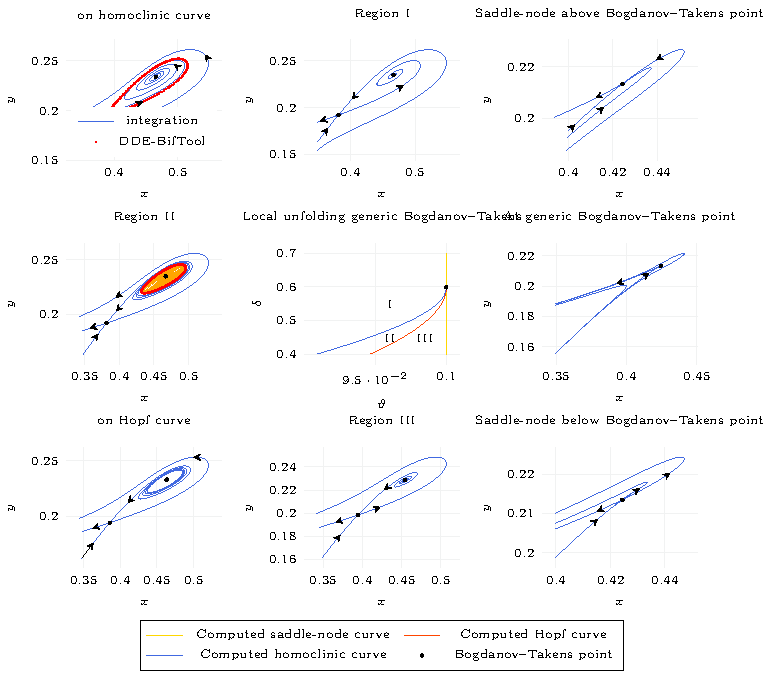
\includegraphics{\imagedir/doubleAlleeEffectSimulation.pdf}
    \caption{Bifurcation diagram near the derived generic Bogdanov-Takens
        points in \cref{sm:eq:neural_network}. In the center we plotted the
        computed codimension one curves emanating from the Bogdanov--Takens
        point using \DDEBIFTOOL with the third-order homoclinic asymptotics
        obtained in \cref{btdde:sec:generic_bt_homoclinic_asymptotics}. The simulations
        surrounding the center plot have been preformed in Julia.}
    \label{sm:fig:double_alle_effect-bifurcation-diagram}
\end{figure}
%
We finish this demonstration by simulating the dynamics near the generic
Bogdanov--Takens point. In \cref{sm:fig:double_alle_effect-bifurcation-diagram}
we created the full local unfolding of the generic Bogdanov--Takens point. Note
that compared with \cite{Jiao2021} the simulation is done with the original
delay differential equations \cref{sm:eq:double_alle_effect_rescaled} and not
with the ordinary differential equations of the reduced system on the center
manifold. We are able to do this since the parameter-dependent center manifold
is locally attractive. In order in integrate the system in the reverse direction, i.e.,
to obtain the orbits in the stable manifold of the equilibria, we multiplied 
the right-hand size of the system in \cref{sm:eq:double_alle_effect_rescaled} by $-1$.
Note that in general this will not provide an accurate approximation at all.
However, since the delay is relatively small, this approximation is accurate
enough for our application. Also, note that the Bogdanov--Takens point still
exists for approximate system. Nonetheless, even without the backward solutions
the bifurcation diagram shows that the numerical analysis obtained in
\DDEBIFTOOL is correct.

Since the code for creating the local unfolding diagram is
rather long we show the code for reproducing the plot simulating the system
near the homoclinic orbit. The code for creating the bifurcation diagram in
\cref{sm:fig:double_alle_effect-bifurcation-diagram} can be found in the
GitHub repository.

\subsubsection{Loading necessary Julia packages}
We start by loading the necessary packages. These are
\begin{itemize}
    \item {\tt DifferentialEquations.jl} A suite for numerically solving differential equations written in Julia.
    \item {\tt GLMakie.jl} For high level plotting on the GPU.
    \item {\tt NonlinearEigenproblems.jl} A nonlinear eigenvalue problem determine a scalar $\lambda$ and a vector $v$ such that $M(\lambda)v=0$. In our case the matrix $M(\lambda)$ will be the characteristic matrix.
    \item {\tt DDEBifTool.jl} We created this very minimalistic package to have some functionality for normal form calculations of DDEs in Julia. Here we use it to calculate the derivatives of the system necessary for {\tt NonlinearEigenproblems.jl}.
    \item {\tt DelimitedFiles.jl} Reading and writing of CSV files.
    \item {\tt PGFPlotsX.jl} A Julia package for creating publication quality figures using the LaTeX library PGFPlots as the backend.
\end{itemize}
\newcommand\pathToJuliaFiles{/home/maikel/Documents/MyPapers/BTPaper/simulation}
\inputminted[firstline=1, lastline=8]{julia}{\pathToJuliaFiles/predator_prey_simulation_article.jl}

\subsubsection{Define system}
Next we define the system to be integrated, a system to approximate the reverse
flow, and also a allocating version used for stability calculations.
\inputminted[firstline=10, lastline=38]{julia}{\pathToJuliaFiles/predator_prey_simulation_article.jl}

\subsubsection{Functions for plotting arrows} \label{sm:eq:arrow_functions}
We define a function the show in which direction the orbits flow, which is
useful when plotting in phase-space. We also define a function to show in
direction of the leading eigenvectors of the characteristic matrix.

\begin{code}
\inputminted[firstline=40, lastline=71]{julia}{\pathToJuliaFiles/predator_prey_simulation_article.jl}
\caption{Functions for plotting arrows.}
\label{sm:lst:arrow_fucntions}
\end{code}

\subsubsection{Define parameters, equilbria}
We define parameters located on the continued homoclinic branch with
\DDEBIFTOOL. Then define the non-trivial equilbria points in
\cref{sm:eq:double_alle_effect_rescaled} which can be derived analytically.
\inputminted[firstline=73, lastline=80]{julia}{\pathToJuliaFiles/predator_prey_simulation_article.jl}

\subsubsection{Plot equilbria and homoclinic orbit}
By plotting the homoclinic orbit obtained with \DDEBIFTOOL we can compare with the numerical simulations. 
\inputminted[firstline=82, lastline=91]{julia}{\pathToJuliaFiles/predator_prey_simulation_article.jl}

\subsubsection{Eigenvectors}
Next, we calculate and plot the leading eigenvectors of the characteristic matrix at the saddle-node bifurcation point.
\inputminted[firstline=93, lastline=105]{julia}{\pathToJuliaFiles/predator_prey_simulation_article.jl}

\subsubsection{Define callback}
Since we are only interested in the flow near the equilbria points we create a
discrete callback to ensure the orbits don't become the large.
\inputminted[firstline=107, lastline=110]{julia}{\pathToJuliaFiles/predator_prey_simulation_article.jl}

\subsubsection{Integrate the system}
Now we define the problem to be integrated and choose the algorithm to be used.
The first of the five numerical simulations below starts near the unstable
eigendirection. We rotated the eigenvector slightly to follow the homoclinic
orbit very close. The rotation value of $\alpha_0$ was actually obtained by using
the bisection method. However, we didn't include this code here. 
\inputminted[firstline=112, lastline=147]{julia}{\pathToJuliaFiles/predator_prey_simulation_article.jl}

\subsubsection{Finish the plot}
Lastly, we add arrows to the obtained solutions using the function
\mintinline{julia}{draw_arrow_on_solution} defined above. Also, we add the
legend and re-plot the equilbria, so that they appear on top.
\inputminted[firstline=149, lastline=161]{julia}{\pathToJuliaFiles/predator_prey_simulation_article.jl}
We should now obtain an interactive figure similar to the left figure in \cref{sm:fig:doubleAlleeEffectHomoclinicSimulation}.
%
\begin{figure}[!ht]
    \centering
    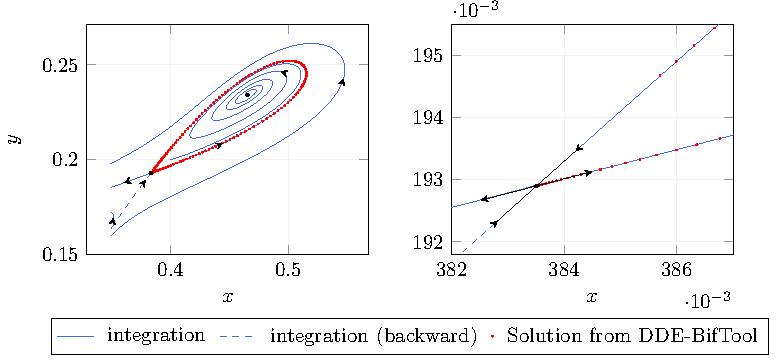
\includegraphics{\imagedir/doubleAlleeEffectHomoclinicSimulation.pdf}
    \caption{Integration of the delayed predator-prey model
        \cref{sm:eq:double_alle_effect_rescaled} at parameter values $(\theta,
        \delta) = (0.094448552842823, 0.447783343351055)$ obtain from
        continuation of the homoclinic curve emanating from the
        Bogdanov--Takens using \DDEBIFTOOL. In the plot to the right
        a close-up near the saddle is given. Additionally, the 
        leading eigenvectors of the characteristic matrix
        are shown.}
    \label{sm:fig:doubleAlleeEffectHomoclinicSimulation}
\end{figure}


\section[Bogdanov--Takens bifurcation in a neural network model]
        {Generic Bogdanov--Takens bifurcation in a neural network model}

In this example we will consider the model 
\begin{equation}
\label{sm:eq:neural_network}
\begin{cases}
\mu\dot{u}_1(t) = -u_1(t) + q_{11}\alpha(u_1(t\text{-}T))-q_{12}u_2(t\text{-}T) + e_1,\\
\mu\dot{u}_2(t) = -u_2(t) + q_{21}\alpha(u_1(t\text{-}T))-q_{22}u_2(t\text{-}T) + e_2,
\end{cases}
\end{equation}
which describes the dynamics of a neural network consisting of an
excitatory and inhibitory neurons \cite{giannakopoulos2001bifurcations}.
The variables and parameters occurring in \cref{sm:eq:neural_network}
have the following neurophysiological meaning:
\begin{itemize}
\item $u_1,u_2:\mathbb{R}\rightarrow\mathbb{R}$ denote the total post-synaptic
potential of the excitatory and inhibitory neuron, respectively.
\item $\mu>0$ is a time constant characterizing the dynamical properties
of cell membrane.
\item $q_{ik}\geq0$ represents the strength of the connection line from
the $k$th neuron to the $i$th neuron.
\item $\alpha:\mathbb{R}\rightarrow\mathbb{R}$ is the transfer function
which describes the activity generation of the excitatory neuron as
a function of its total potential $u_1$. The function $\alpha$
is smooth, increasing and has an unique turning point at $u_1 = \theta$.
The transfer function corresponding to the inhibitory neuron is assumed
to be the identity.
\item $T\geq0$ is a time delay reflecting synaptic delay, axonal and dendritic
propagation time.
\item $e_1$ and $e_2$ are external stimuli acting on the excitatory
and inhibitory neuron, respectively.
\end{itemize}

Following \cite{giannakopoulos2001bifurcations} we consider equation \cref{sm:eq:neural_network} with
\begin{align*}
\alpha(u_1) & = \frac{1}{1 + e^{-4u_1}}-\frac{1}{2},\qquad q_{11} = 2.6,\qquad q_{21} = 1.0,\qquad q_{22} = 0.0,\\
\mu & = 1.0,\qquad T = 1.0,\qquad e_2 = 0.0,
\end{align*}
and $Q: = q_{12},\,E: = e_1$ as bifurcation parameters. Substituting
into \cref{sm:eq:neural_network} yields
\begin{equation}
\label{sm:eq:neural_network_subs}
\begin{cases}
\dot{u}_1(t) = -u_1(t) + 2.6\alpha(u_1(t - 1))-Qu_2(t - 1) + E,\\
\dot{u}_2(t) = -u_2(t) + \alpha(u_1(t - 1)).
\end{cases}
\end{equation}
Notice that for any steady-state we have the symmetry
\begin{equation}
\label{sm:eq:neuralNetworkSymmetry}
    (u_1,u_2,E)\rightarrow(-u_1,-u_2,-E).
\end{equation}
It is easy to explicitly derive that
the system has a double eigenvalue zero for
\begin{equation}
\left\{
\begin{aligned}
    u_1(t) &= \frac14 \log\left(\frac{8 - \sqrt{39}}5\right) \approx -0.2617, \\
    u_2(t) &= -\frac12 \sqrt{\frac{3}{13}} \approx -0.2402, \\
    Q &= \frac{13}{10}, \\
    E &= \frac{\sqrt{39} - 10\atanh \sqrt{\frac{3}{13}}}{20} \approx 0.0505.
\end{aligned}
\right.
\end{equation}

\begin{remark} 
    The \MATLAB files for this demonstration can be found in the directory
    \mintinline[breaklines,breakafter=/]{MATLAB}{demos/tutorial/VII/neural_network_model} relative to the main
    directory of the \DDEBIFTOOL package. Here, we omit the code to generate the
    system file. We assume that the system file
    \mintinline{MATLAB}{sym_neural_network_mf.m} has been
    generated with the script \mintinline{MATLAB}{sym_neural_network.m}. Also, we assume
    that the \DDEBIFTOOL package has been loaded as in
    \cref{sm:lst:searchpath}. The code in
    \crefrange{sm:sec:neural_network_model:pars_and_funcs}{sm:sec:neural_network_model:bifurcation_diagramII}
    highlights the important parts of the file
    \mintinline{MATLAB}{neural_network_model.m}. 
\end{remark}

\subsection{Set parameter names and funcs structure} 
\label{sm:sec:neural_network_model:pars_and_funcs}
As in the previous example, we set the parameter names and define the \mintinline{MATLAB}{funcs} structure.
\inputminted[firstline=28, lastline=39]{MATLAB}{\pathToDDEBifToolDemos/neural_network_model/neural_network_model.m}

\subsection{Set parameter range}
Since we are only interested here in the local unfolding we restrict the
allowed parameter range for the unfolding parameters. In practice one may have
physical restrictions which must be satisfied. Additionally, we also limit the
maximum allowed step size during continuation. By doing so we obtain more refined
data to compare against our predictors.
\inputminted[firstline=41, lastline=44]{MATLAB}{\pathToDDEBifToolDemos/neural_network_model/neural_network_model.m}

\subsection{Stability and coefficients of the generic Bogdanov--Takens point}
We manually construct a steady-state at the generic Bogdanov--Takens point.
\inputminted[firstline=46, lastline=56]{MATLAB}{\pathToDDEBifToolDemos/neural_network_model/neural_network_model.m}
The \MATLAB console shows the following output.
\begin{minted}{shell-session}
ans =

   1.0e-07 *

   0.548156278544666
  -0.548156314155979
\end{minted}
The eigenvalues confirm that the point under consideration is indeed (an
approximation to) a Bogdanov--Takens point. Furthermore, the remaining eigenvalues have
negative real parts. Next, we calculate the normal form coefficients, the
time-reparametrization, and the transformation to the center manifold with the
function \mintinline{MATLAB}{nmfm_bt}, which implements the coefficients as derived in
\cref{btdde:sec:generic_bogdanov-takens}. For this we need to set the argument
\mintinline{MATLAB}{free_pars} to the unfolding parameter $(Q,E)$. These
coefficients will be used to start the continuation of the codimension one branches
emanating from the Bogdanov--Takens point.
\inputminted[firstline=58, lastline=62]{MATLAB}{\pathToDDEBifToolDemos/neural_network_model/neural_network_model.m}
The \MATLAB console shows the following output.
\begin{minted}{shell-session}
ans =

  struct with fields:

          a: -0.190382124055415
          b: -0.951910620277072
  theta1000: -0.546026508575597
  theta0001: 1.473611111111115
        K10: [2x1 double]
        K01: [2x1 double]
        K02: [2x1 double]
        K11: [2x1 double]
        K03: [2x1 double]
       phi0: [1x1 struct]
       phi1: [1x1 struct]
      h0010: [1x1 struct]
      h0001: [1x1 struct]
      h2000: [1x1 struct]
      h1100: [1x1 struct]
      h0200: [1x1 struct]
      h1010: [1x1 struct]
      h1001: [1x1 struct]
      h0110: [1x1 struct]
      h0101: [1x1 struct]
      h0002: [1x1 struct]
      h0011: [1x1 struct]
      h3000: [1x1 struct]
      h2100: [1x1 struct]
      h1101: [1x1 struct]
      h2001: [1x1 struct]
      h0003: [1x1 struct]
      h1002: [1x1 struct]
      h0102: [1x1 struct]
          K: @(beta1,beta2)K10*beta1+K01*beta2+1/2*K02*beta2.^2
                +K11*beta1.*beta2+1/6*K03*beta2^3
          H: [function_handle]
\end{minted}
Since the sign of $ab$ is positive we expect to find unstable periodic orbits nearby the 
Bogdanov--Takens point.

\subsection{Comparing profiles of computed and predicted homoclinic orbits}
To test the homoclinic asymptotics from
\cref{btdde:sec:generic_bt_homoclinic_asymptotics} we compare the first and third
order asymptotics to the Newton corrected solution. For this we use the 
function \mintinline[breaklines,breakafter=_]{MATLAB}{C1branch_from_C2point}. This function returns a branch, which
by default returns two initial corrected approximations in order to start continuation of the
codimension one curve under consideration. By setting the argument
\mintinline{MATLAB}{'predictor'} to \mintinline{MATLAB}{true} the approximations are left uncorrected.
To make the comparison visually clear we set the perturbation parameter 
$\epsilon=0.25$ (\mintinline{MATLAB}{step = 0.25} in the code below).
The code below produces \cref{sm:fig:DoubleAlleeEffectCompareProfiles}.
The difference between the two approximations is clearly noticeable. While
the first order asymptotics is close to the Newton corrected solution, the third
order asymptotics is indistinguishable at this scale from the Newton corrected
solution.
\inputminted[firstline=64, lastline=82]{MATLAB}{\pathToDDEBifToolDemos/neural_network_model/neural_network_model.m}
\begin{figure}[ht]
    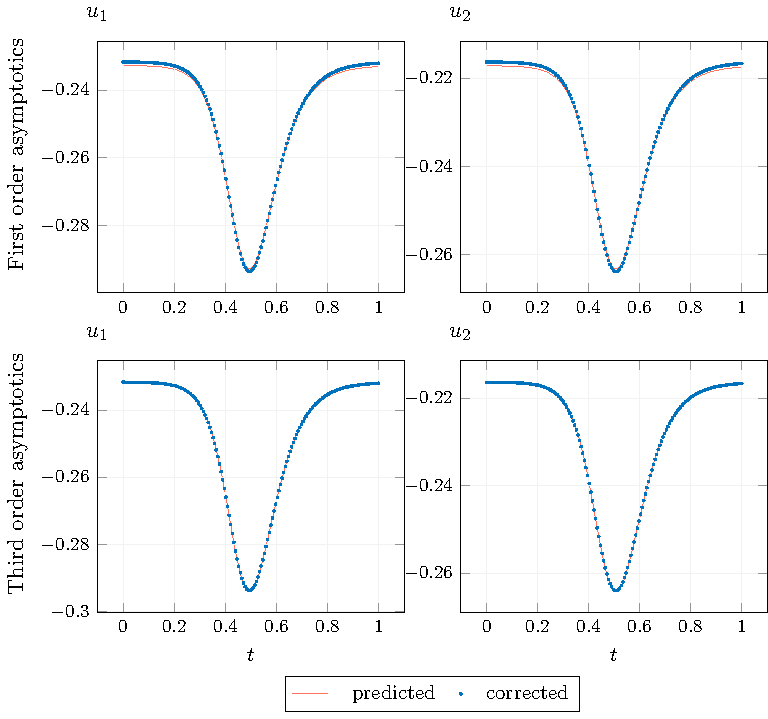
\includegraphics{\imagedir/NeuralNetworkCompareProfiles.pdf}
    \caption{Comparison between the first and third-order asymptotics from
    \cref{btdde:sec:generic_bt_homoclinic_asymptotics} near the generic
        Bogdanov--Takens bifurcation in \cref{sm:eq:neural_network} with the
        perturbation parameter set to $\epsilon=0.25$.}
    \label{sm:fig:NeuralNetworkCompareProfiles}
\end{figure}

\label{sm:sec:neural_network_model:continuation}
\subsection{Continuation of the codimension one curves emanating}
To continue the three codimension one curves emanating from the generic
Bogdanov--Takens we can simply use the function
\mintinline[breaklines,breakafter=_]{MATLAB}{C1branch_from_C2point}, as show in the code below. To monitor the
continuation process the argument \mintinline{MATLAB}{plot} must be set \mintinline{MATLAB}{1}.
The most important setting is the perturbation parameter (or multiple),
\mintinline{MATLAB}{step} in the code below. If left out, default stepsizes are defined.
However, depending on the problem no convergence may then be obtained.
\inputminted[firstline=84, lastline=102]{MATLAB}{\pathToDDEBifToolDemos/neural_network_model/neural_network_model.m}

\subsection{Predictors of the codimension one curves emanating from the Bogdanov--Takens point}
Before we provide the bifurcation diagram in the next section we first obtain the predictors
for the codimension one curves. For this we again use the function
\mintinline[breaklines,breakafter=_]{MATLAB}{C1branch_from_C2point}. We set the argument \mintinline{MATLAB}{predictor} to \mintinline{MATLAB}{1}
and provide a range of perturbation parameters.
\inputminted[firstline=121, lastline=133]{MATLAB}{\pathToDDEBifToolDemos/neural_network_model/neural_network_model.m}
In the last part of the code above we added the asymptotics obtained from \cite{Jiao2021}.

\subsection{Bifurcation diagram}
The code below produce (a figure similar to) \cref{sm:fig:DoubleAlleeEffectCompareParameters}.
%% Plot the bifurcation curves with predictors
\inputminted[firstline=135, lastline=156]{MATLAB}{\pathToDDEBifToolDemos/neural_network_model/neural_network_model.m}
%
\begin{figure}[ht]
    \centering
    \includetikzscaled{NeuralNetworkCompareParameters}
    \caption{Bifurcation diagram near the derived generic Bogdanov-Takens point in
        \cref{sm:eq:neural_network} comparing computed codimension one curves using
        \DDEBIFTOOL with the third-order homoclinic parameter asymptotics obtained
        in \cref{btdde:sec:generic_bt_homoclinic_asymptotics}.}
    \label{sm:fig:NeuralNetworkCompareParameters}
\end{figure}

\subsection{Compare homoclinic solutions in phase-space}
To obtain an impression of the third-order homoclinic asymptotics in
phase-space we compare the correct and uncorrected homoclinic solution
with the perturbation parameter ranging from $0.1$ to $0.3$.
The code below results in \cref{sm:fig:NeuralNetworkCompareOrbitsPhaseSpace}.
We see that the corrected and predicted homoclinic orbits are nearly identical.
\inputminted[firstline=158, lastline=174]{MATLAB}{\pathToDDEBifToolDemos/neural_network_model/neural_network_model.m}
%
\begin{figure}[ht]
    \centering
    \includetikzscaled{NeuralNetworkCompareOrbitsPhaseSpace}
    \caption{Plot comparing the third-order homoclinic asymptotics from
        \cref{btdde:sec:generic_bt_homoclinic_asymptotics} near the generic
        Bogdanov--Takens bifurcation in \cref{sm:eq:neural_network} with the
        Newton correct homoclinic solutions in $(u_1,u_2)$ phase-space.}
    \label{sm:fig:NeuralNetworkCompareOrbitsPhaseSpace}
\end{figure}

\subsection{Convergence plot}
Using the function from \cref{sm:lst:convergence_plot} we create a log-log
convergence plot comparing the convergence order of the first and thrid order
homoclinic asymptotics from \cref{btdde:sec:generic_bt_homoclinic_asymptotics}.
The code below yields \cref{sm:fig:NeuralNetworkConvergencePlot}.
\inputminted[firstline=176, lastline=187]{MATLAB}{\pathToDDEBifToolDemos/neural_network_model/neural_network_model.m}
\begin{figure}[ht]
    \centering
    \includetikz{NeuralNetworkConvergencePlot}
        \caption{On the abscissa is the approximation to the amplitude $A_0$ and on
        the ordinate the relative error $\delta$ between the constructed solution
        \mintinline{MATLAB}{hcli_pred} to the defining system for the homoclinic orbit
        and the Newton corrected solution \mintinline{MATLAB}{hcli_corrected}.}
    \label{sm:fig:NeuralNetworkConvergencePlot}
\end{figure}

\subsection{Continuation of the codimension one curves emanating from the second Bogdanov--Takens point}
For completeness, we also continue the codimension one curves emanating from
the second Bogdanov--Takens point, which exists due to the symmetry
\cref{sm:eq:neuralNetworkSymmetry}. Of course, we could just use the symmetry
instead of computing the curves numerically. However, we use it as an
additional verification of our derived asymptotics. The code below defines the
second Bogdanov--Takens point, calculates the stability, and continues the Hopf
and homoclinic bifurcation curves.
\inputminted[firstline=189, lastline=216]{MATLAB}{\pathToDDEBifToolDemos/neural_network_model/neural_network_model.m}

\subsection{Bifurcation diagram with two Bogdanov--Takens points}
\label{sm:sec:neural_network_model:bifurcation_diagramII}
Now that we continued the Hopf and homoclinic bifurcation curves emanating from
the second Bogdanov--Takens point we can reconstruct the bifurcation diagram
given in \cite[Figure 7]{giannakopoulos2001bifurcations}. The code below
results into a similar figure as \cref{sm:fig:NeuralNetworkCompareParametersII} in \MATLAB.
\inputminted[firstline=218, lastline=245]{MATLAB}{\pathToDDEBifToolDemos/neural_network_model/neural_network_model.m}
\begin{figure}[ht]
    \centering
    \includetikzscaled{NeuralNetworkCompareParametersII}
    \caption{Reconstruction of the bifurcation diagram given in \cite[Figure
        7]{giannakopoulos2001bifurcations}. We could have used the symmetry
        \cref{sm:eq:neuralNetworkSymmetry} instead of computing the additional
        curves numerically. However, it provides us an additional verification of
        our derived asymptotics.}
    \label{sm:fig:NeuralNetworkCompareParametersII}
\end{figure}

\subsection{Simulation with {\tt DifferentialEquations.jl}}
Here we will preform two simulations. The first simulation will be at the
double homoclinic orbits, which will confirm the continuation of both
homoclinic orbits and is also ascetically pleasing, see \cref{sm:fig:NeuralNetworkSimulationHomoclinic}. The second simulation will
be in the region where there should be unstable periodic orbits, see \cref{sm:fig:NeuralNetworkPeriodicSimulation}.

\begin{figure}[ht]
    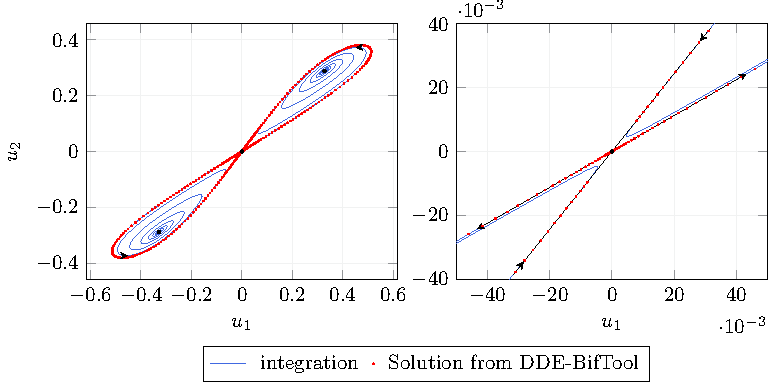
\includegraphics{\imagedir/NeuralNetworkDoubleHomoclinicSimulation.pdf}
    \caption{Comparing the computed double homoclinic orbit in \cref{sm:eq:neural_network}
    with \DDEBIFTOOL with the solution obtain from numerical simulation with Julia.
    In the right plot is a close-up near the equilibrium at the origin. Also, the
    leading stable and unstable eigenvectors of the characteristic matrix are plotted. We see the numerical integrated solution
    intersects all the red points from the solution from \DDEBIFTOOL.}
    \label{sm:fig:NeuralNetworkSimulationHomoclinic}
\end{figure}

\begin{figure}[ht]
    \centering
    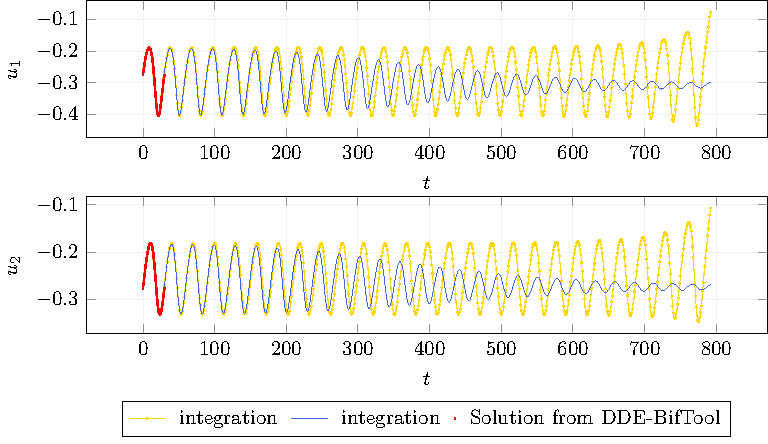
\includegraphics{\imagedir/NeuralNetworkPeriodicSimulation.pdf}
    \caption{Comparing a computed periodic orbit in \cref{sm:eq:neural_network}
        with \DDEBIFTOOL at $(Q,E)=(1.476442865781454, 0.0)$ with the solution
        obtain from numerical simulation with Julia near the periodic orbit.
        The yellow dotted line has the constant history function $(u_1,u_2) =
        (-0.274863341578762, -0.27715979849863204)$ slightly below the periodic
        orbit.  The blue line has the constant history function $(u_1,u_2) =
        (-0.274863341578762, -0.276969798498632)$, a point on the periodic
        orbit (red dots) located with \DDEBIFTOOL.
    }
    \label{sm:fig:NeuralNetworkPeriodicSimulation}
\end{figure}

\subsubsection{Loading necessary Julia packages}
We start by loading the necessary packages.
\begin{listing}[H]
\inputminted[firstline=1, lastline=6]{julia}{\pathToJuliaFiles/neural_network_model_simulation_article.jl}
\caption{Loading Julia packages for simulation in \cref{sm:eq:neural_network}.}
\label{sm:lst:neuralNetworkLoadingPacakges}
\end{listing}
%
In the previous demonstration we were able to derive the equilbria
analytically.  Here we will solve for the equilbria numerically with the
packages {\tt IntervalArithmetic.jl} \cite{IntervalArithmetic} and  {\tt
IntervalRootFinding.jl} \cite{IntervalRootFinding}.

\subsubsection{Define system}
We define the system to be integrated, a system to approximate the reverse
flow, and also a allocating version used for stability calculations.
\inputminted[firstline=8, lastline=27]{julia}{\pathToJuliaFiles/neural_network_model_simulation_article.jl}

\subsubsection{Functions for plotting arrows}
We define a function the show in which direction the orbits flow, which is
useful when plotting in phase-space. We also define functions to show in
direction of the leading eigenvectors of the characteristic matrix.
The code is shown in \cref{sm:lst:arrow_fucntions}.

\subsubsection{Create figure with several axes}
We create a figure containing multiple axis in which we will plot the bifurcation diagram and
the homoclinic and periodic orbits.
\inputminted[firstline=63, lastline=73]{julia}{\pathToJuliaFiles/neural_network_model_simulation_article.jl}

\subsubsection{Plot bifurcation diagram in the middle}
Loading the continued bifurcation curves obtain with \DDEBIFTOOL and plot these in the middle axis.
This should give a similar bifurcation diagram as in \cref{sm:fig:NeuralNetworkCompareParametersII}.
\inputminted[firstline=76, lastline=102]{julia}{\pathToJuliaFiles/neural_network_model_simulation_article.jl}

\subsubsection{Simulation at the double homoclinic orbit}
In the code below we integrate at parameter values $(Q,E)=1.459868437376222,0$, i.e.,
where we located the double homoclinic orbit. We start by locating the three equilibria
points. Note that by the symmetry we actually only need to solve for one of them.
We calculate the stability of the equilbria and filter out the leading stable and unstable
eigenvectors from the characteristic matrix of the saddle-node piont. 
The rest of the code should be pretty straight forward,
since it is very similar as in the simulation in the previous demonstration.
After running this code we should obtain a similar plot as in
the left plot of \cref{sm:fig:NeuralNetworkSimulationHomoclinic}.
\inputminted[firstline=105, lastline=166]{julia}{\pathToJuliaFiles/neural_network_model_simulation_article.jl}

\subsubsection{Simulation near an unstable periodic orbit}
To show by integration the existence of an unstable periodic orbit we first
located a periodic orbit in \DDEBIFTOOL. This can be done by continuing a
branch of periodic orbits emanating from a point on the continued Hopf curve.
Then we load the profiles of the periodic orbits into Julia and start
integration near the perioidic orbits.  After running the code below we should
obtain a similar plot as in
\cref{sm:fig:NeuralNetworkPeriodicSimulation}.
\inputminted[firstline=169, lastline=208]{julia}{\pathToJuliaFiles/neural_network_model_simulation_article.jl}




\section[the Van der Pol oscillator with delay feedback]
        {Transcritical Bogdanov--Takens bifurcation in the Van der Pol oscillator with delay feedback}
We consider the Van der Pol oscillator with delay feedback \cite{jiang2007bogdanov}
given by 
\begin{equation}
\ddot{x}(t) + \epsilon(x^2(t)-1)\dot{x}(t) + x(t) = \epsilon g(x(t-\tau))\label{sm:eq:dde_vanderPol}
\end{equation}
where $\epsilon>0$ is a parameter, $\tau>0$ is a delay and $g:\mathbb{R}\rightarrow\mathbb{R}$
is a smooth function with $g(0) = 0$ and $g'(0)\neq0$. We rewrite
the Van der Pol equation \cref{sm:eq:dde_vanderPol} as
\begin{equation}
\label{sm:eq:vanderPolOscillator}
\begin{cases}
    \dot{x}_1 = x_2,\\
    \dot{x}_2 = \epsilon g(x_1(t-\tau))-\epsilon(x_1^2-1)x_2-x_1.
\end{cases}
\end{equation}
Rescaling time with $t\rightarrow\dfrac{t}{\tau}$ to normalize the
delay yields
\begin{equation}
\label{sm:eq:vanderPolOscillatorRescaled}
\begin{cases}
\dot{x}_1 = \tau x_2,\\
\dot{x}_2 = \tau\left(\epsilon g(x_1(t-1))-\epsilon(x_1^2-1)x_2-x_1\right).
\end{cases}
\end{equation}
In this allows is to treat $\tau$ as a bifurcation parameter.

Following \cite{jiang2007bogdanov}, we consider \cref{sm:eq:dde_vanderPol} with
\[
g(x) = \frac{e^x-1}{c_1e^x + c_2},
\]
where $c_1 = \dfrac{1}{4}$ and $c_2 = \dfrac{1}{2}$. Then the trivial
equilibrium undergoes a transcritical Bogdanov--Takens bifurcation at parameter
values $(\epsilon,\tau) = (0.75,0.75)$, \cite{jiang2007bogdanov} and the
supplement. 

\begin{remark}
    The \MATLAB files for this demonstration can be found in the directory
    \mintinline[breaklines,breakafter=/]{MATLAB}{demos/tutorial/VII/vdpo_bt_transcritical} relative to the main
    directory of the \DDEBIFTOOL package. Here, we omit the code to generate a
    system file. The system file \mintinline{MATLAB}{sym_vdpo_mf.m} has been generated
    with the script \mintinline{MATLAB}{sym_vdpo_mf.m}. Also, we assume that the
    \DDEBIFTOOL package has been loaded as in \cref{sm:lst:searchpath}. The
    code in
    \crefrange{sm:sec:vpdo:pars_and_funcs}{sm:sec:vdpo:convergence_plot}
    highlights the important parts of the file
    \mintinline{MATLAB}{vanderPolOscillator.m}. 
\end{remark}

\subsection{Set parameter names and funcs structure}
\label{sm:sec:vpdo:pars_and_funcs}
As in the previous example, we set the parameter names and define the \mintinline{MATLAB}{funcs} structure.
\inputminted[firstline=31, lastline=37]{MATLAB}{\pathToDDEBifToolDemos/vdpo_bt_transcritical/vanderPolOscillator.m}

\subsection{Set parameter range}
Since we are only interested here in the local unfolding we restrict the
allowed parameter range for the unfolding parameters. In practice one may have
physical restrictions which must be satisfied. Additionally, we also limit the
maximum allowed step size during continuation. By doing so we obtain more refined
data to compare against our predictors.
\inputminted[firstline=39, lastline=42]{MATLAB}{\pathToDDEBifToolDemos/vdpo_bt_transcritical/vanderPolOscillator.m}

\subsection{Stability and coefficients of the transcritical Bogdanov--Takens point}
We manually construct a steady-state at the transcritical Bogdanov--Takens
point and calculate its stability.
\inputminted[firstline=44, lastline=55]{MATLAB}{\pathToDDEBifToolDemos/vdpo_bt_transcritical/vanderPolOscillator.m}

The \MATLAB console shows the following output.
\begin{minted}{shell-session}
ans =

   1.0e-07 *

       0.6223
      -0.6223

\end{minted}
The eigenvalues confirm that the point under consideration is indeed (an
approximation to) a Bogdanov--Takens point. Furthermore, the remaining eigenvalues have
negative real parts. Next, we calculate the normal form coefficients, the
time-reparametrization, and the transformation to the center manifold with the
function \mintinline{MATLAB}{nmfm_bt}, which implements the coefficients as derived in
\cref{btdde:sec:transcritical-Bogdanov-Takens}. For this we need to set the argument
\mintinline{MATLAB}{free_pars} to the unfolding parameter $(Q,E)$. These
coefficients will be used to start the continuation of the codimension one branches
emanating from the Bogdanov--Takens point. Also, since we are in the transcritical case,
we set the argument \mintinline{matlab}{generic_unfolding} to \mintinline{matlab}{false}.
\inputminted[firstline=57, lastline=60]{MATLAB}{\pathToDDEBifToolDemos/vdpo_bt_transcritical/vanderPolOscillator.m}

The \MATLAB console shows the following output.
\begin{minted}{shell-session}
ans =

  struct with fields:

          a: 0.1304
          b: -0.2949
  theta1000: 0.0780
  theta0010: -21.1293
  theta0001: -0.3811
       phi0: [1x1 struct]
       phi1: [1x1 struct]
      h2000: [1x1 struct]
      h1100: [1x1 struct]
      h0200: [1x1 struct]
      h3000: [1x1 struct]
      h2100: [1x1 struct]
        K10: [2x1 double]
        K01: [2x1 double]
        K02: [2x1 double]
        K11: [2x1 double]
        K20: [2x1 double]
      h1010: [1x1 struct]
      h1001: [1x1 struct]
      h0110: [1x1 struct]
      h0101: [1x1 struct]
      h2010: [1x1 struct]
      h1110: [1x1 struct]
      h2001: [1x1 struct]
      h1101: [1x1 struct]
      h1002: [1x1 struct]
      h0102: [1x1 struct]
      h1020: [1x1 struct]
      h0120: [1x1 struct]
      h1011: [1x1 struct]
      h0111: [1x1 struct]
          K: @(beta1,beta2)K10*beta1+K01*beta2+1/2*K20*beta1^2
                    +K11*beta1*beta2+1/2*K02*beta2^2
          H: [function_handle]
\end{minted}
Since the sign of $ab$ is negative we expect to find stable periodic orbits nearby the 
Bogdanov--Takens point.

\subsection{Comparing profiles of computed and predicted homoclinic orbits}
To test the homoclinic asymptotics from
\cref{btdde:sec:generic_bt_homoclinic_asymptotics} we compare the first and third
order asymptotics to the Newton corrected solution. For this we use the 
function \mintinline[breaklines,breakafter=_]{MATLAB}{C1branch_from_C2point}. This function returns a branch, which
by default returns two initial corrected approximations in order to start continuation of the
codimension one curve under consideration. By setting the argument
\mintinline{MATLAB}{'predictor'} to \mintinline{MATLAB}{true} the approximations are left uncorrected.
To make the comparison visually clear we set the perturbation parameter 
$\epsilon=0.1$ (\mintinline{MATLAB}{step = 0.1} in the code below).
The code below produces \cref{sm:fig:VDPOCompareProfiles}.
The difference between the two approximations is clearly noticeable. While
the first order asymptotics is close to the Newton corrected solution, the third
order asymptotics is indistinguishable at this scale from the Newton corrected
solution.
\inputminted[firstline=63, lastline=87]{MATLAB}{\pathToDDEBifToolDemos/vdpo_bt_transcritical/vanderPolOscillator.m}

\begin{figure}[ht]
    \centering
    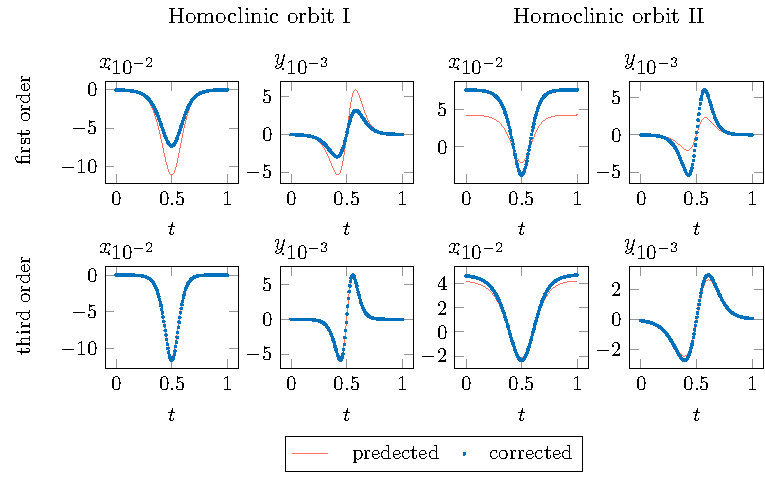
\includegraphics{\imagedir/VDPOCompareProfiles.pdf}
    \caption{Comparison between the first and third-order homoclinic asymptotics from
    \cref{btdde:sec:transcritical_bt_homoclinic_asymptotics} near the transcritical
        Bogdanov--Takens bifurcation in \cref{sm:eq:vanderPolOscillatorRescaled} with the
        perturbation parameter set to $\epsilon=0.1$.}
    \label{sm:fig:VDPOCompareProfiles}
\end{figure}

\subsection{Continuation of the codimension one curves emanating}
To continue the three codimension one curves emanating from the generic
Bogdanov--Takens we can simply use the function
\mintinline[breaklines,breakafter=_]{MATLAB}{C1branch_from_C2point}, as show in the code below. To monitor the
continuation process the argument \mintinline{MATLAB}{plot} must be set \mintinline{MATLAB}{1}.
The most important setting is the perturbation parameter (or multiple),
\mintinline{MATLAB}{step} in the code below. If left out, default stepsizes are defined.
However, depending on the problem no convergence may then be obtained.
\inputminted[firstline=89, lastline=113]{MATLAB}{\pathToDDEBifToolDemos/vdpo_bt_transcritical/vanderPolOscillator.m}

\subsection{Predictors of the codimension one curves emanating from the Bogdanov--Takens point}
Before we provide the bifurcation diagram in the next section we first obtain the predictors
for the codimension one curves. For this we again use the function
\mintinline[breaklines,breakafter=_]{MATLAB}{C1branch_from_C2point}. We set the argument \mintinline{MATLAB}{predictor} to \mintinline{MATLAB}{1}
and provide a range of perturbation parameters.
\inputminted[firstline=135, lastline=154]{MATLAB}{\pathToDDEBifToolDemos/vdpo_bt_transcritical/vanderPolOscillator.m}

\subsection{Bifurcation diagram}
The code below produce (a figure similar to) \cref{sm:fig:DoubleAlleeEffectCompareParameters}.
\inputminted[firstline=156, lastline=182]{MATLAB}{\pathToDDEBifToolDemos/vdpo_bt_transcritical/vanderPolOscillator.m}
%
\begin{figure}[ht]
    \centering
    \includetikzscaled{vanderPolOscillatorCompareParameters}
    \caption{Bifurcation diagram near the derived transcritical Bogdanov-Takens point in
        \cref{sm:eq:vanderPolOscillatorRescaled} comparing computed codimension one curves using
        \DDEBIFTOOL with the third-order homoclinic parameter asymptotics obtained
        in \cref{btdde:sec:transcritical_bt_homoclinic_asymptotics}.}
    \label{sm:fig:VDPOCompareParameters}
\end{figure}

\subsection{Compare homoclinic solutions in phase-space}
To obtain an impression of the third-order homoclinic asymptotics in
phase-space we compare the correct and uncorrected homoclinic solution
with the perturbation parameter ranging from $0.01$ to $0.03$.
The code below produce (a figure similar to) \cref{sm:fig:VDPOCompareOrbitsPhaseSpace}.
We see that the corrected and predicted homoclinic orbits are nearly identical.
\inputminted[firstline=203, lastline=230]{MATLAB}{\pathToDDEBifToolDemos/vdpo_bt_transcritical/vanderPolOscillator.m}
%
\begin{figure}[ht]
    \centering
    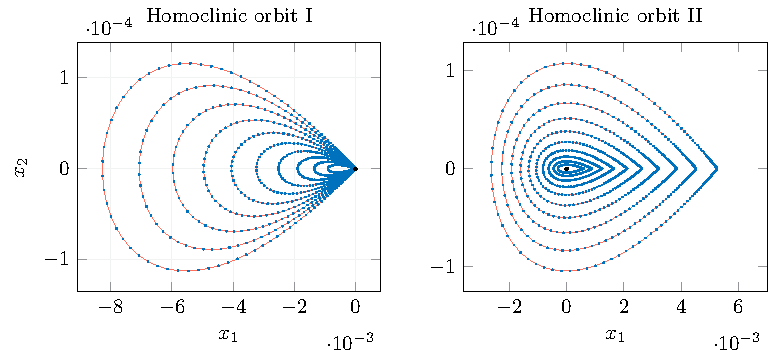
\includegraphics{\imagedir/VDPOCompareOrbitsPhaseSpace.pdf} \\
    \vspace*{20pt}
    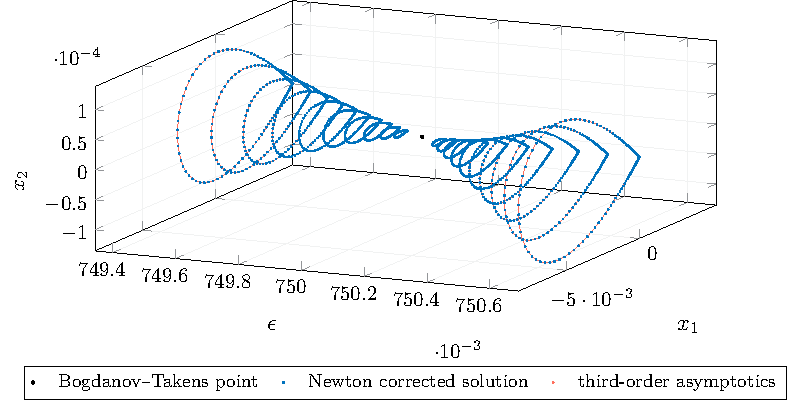
\includegraphics{\imagedir/VDPOCompareOrbitsPhaseSpaceBottom.pdf}
    \caption{Plot comparing the third-order homoclinic asymptotics from
        \cref{btdde:sec:transcritical_bt_homoclinic_asymptotics} near the
        transcritical Bogdanov--Taken in
        \cref{sm:eq:vanderPolOscillatorRescaled} with the Newton correct
        homoclinic solutions phase-space with the perturbation parameter
        $\epsilon$ ranging from $0.01$ to $0.03$.}
    \label{sm:fig:VDPOCompareOrbitsPhaseSpace}
\end{figure}

\subsection{Convergence plot}
\label{sm:sec:vdpo:convergence_plot}
Using the function from \cref{sm:lst:convergence_plot} we create a log-log
convergence plot comparing the convergence order of the first and thrid order
homoclinic asymptotics from \cref{btdde:sec:transcritical_bt_homoclinic_asymptotics}.
The code below yields \cref{sm:fig:VDPOConvergencePlot}.
\inputminted[firstline=232, lastline=243]{MATLAB}{\pathToDDEBifToolDemos/vdpo_bt_transcritical/vanderPolOscillator.m}
%
\begin{figure}[ht]
    \centering
    \includetikz{VDPOConvergencePlot}
        \caption{On the abscissa is the approximation to the amplitude $A_0$ and on
        the ordinate the relative error $\delta$ between the constructed solution
        \mintinline{MATLAB}{hcli_pred} to the defining system for the homoclinic orbit
        and the Newton corrected solution \mintinline{MATLAB}{hcli_corrected}.}
    \label{sm:fig:VDPOConvergencePlot}
\end{figure}

\subsection{Simulation with {\tt DifferentialEquations.jl}}
Here we will preform four simulations. The first two simulations will be at two
homoclinic orbits located on the two homoclinic curves emanating from the
transcritical Bogdanov--Takens point continued with \DDEBIFTOOL, see
\cref{sm:fig:VDPOSimulationHomoclinic}. The second two simulations will be in
the regions where there should be stable periodic orbits, see
\cref{sm:fig:VDPOPeriodicSimulation}.

\begin{figure}[ht]
    \centering
    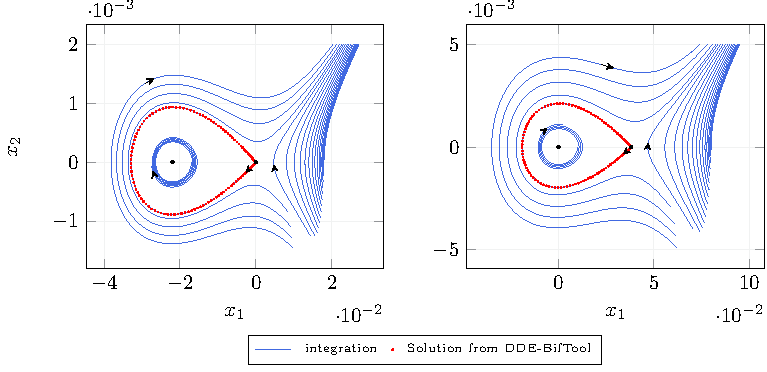
\includegraphics{\imagedir/VDPOHomoclinicSimulation.pdf}
    \caption{Comparing the computed homoclinic orbits in \cref{sm:eq:vanderPolOscillatorRescaled}
    with \DDEBIFTOOL with the solution obtain from numerical simulation with Julia.
    We see the numerical integrated solution
    going through all the red points from the solution from \DDEBIFTOOL.}
    \label{sm:fig:VDPOSimulationHomoclinic}
\end{figure}

\begin{figure}[ht]
    \centering
    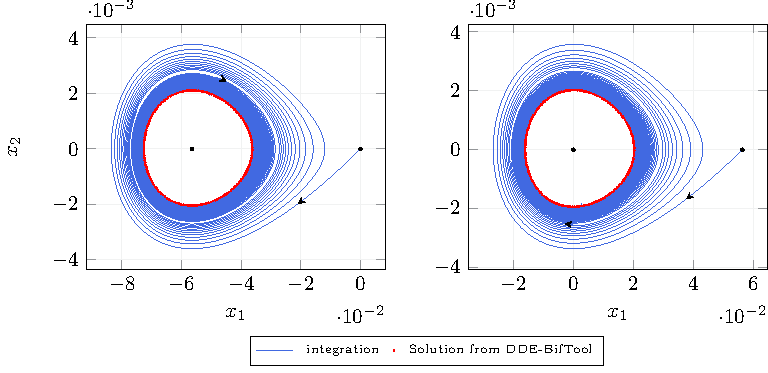
\includegraphics{\imagedir/VDPOPeriodicSimulation.pdf}
    \caption{Comparing the computed periodic orbits in \cref{sm:eq:vanderPolOscillatorRescaled}
    with \DDEBIFTOOL with the solution obtain from numerical simulation with Julia.
    We see the numerical integrated solution
    going through all the red points from the solution from \DDEBIFTOOL.}
    \label{sm:fig:VDPOPeriodicSimulation}
\end{figure}

\subsubsection{Loading necessary Julia packages}
Since we do not have analytical expression we load the same Julia packges as in
the previous demonstration, see \cref{sm:lst:neuralNetworkLoadingPacakges}.

\subsubsection{Define system}
We define the system to be integrated and also and allocating version used for
stability calculations.
\inputminted[firstline=8, lastline=30]{julia}{\pathToJuliaFiles/vdpo_simulation_article.jl}

\subsubsection{Functions for plotting arrows}
We define a function the show in which direction the orbits flow, which is
useful when plotting in phase-space. We also define functions to show in
direction of the leading eigenvectors of the characteristic matrix.
The code is shown in \cref{sm:lst:arrow_fucntions}.

\subsubsection{Function for creating streamlines plot}
To obtain an impression of the flow near transcritical Bogdanov--Takens point
we create a streamlines function. This is particularly useful for seeing the
flow around the stable manifold of the saddle-note.
\inputminted[firstline=65, lastline=77]{julia}{\pathToJuliaFiles/vdpo_simulation_article.jl}

\subsubsection{Create figure with several axes}
We create a figure containing multiple axis in which we will plot 
the two homoclinic and two periodic orbits.
\inputminted[firstline=79, lastline=84]{julia}{\pathToJuliaFiles/vdpo_simulation_article.jl}

\subsubsection{Define parameters, equilbria}
We define parameters located on the continued homoclinic branch with
\DDEBIFTOOL. Then calculate the equilbria points in
\cref{sm:eq:vanderPolOscillatorRescaled} near the transcritical
Bogdanov--Takens point.
\inputminted[firstline=86, lastline=93]{julia}{\pathToJuliaFiles/vdpo_simulation_article.jl}

\subsubsection{Plot equilbria and homoclinic orbit}
By plotting the homoclinic orbit obtained with \DDEBIFTOOL located at parameter
values $(\epsilon_0, \tau_0) =  (0.752774810893411,0.754736729675371)$ we can
compare with the numerical simulations.
\inputminted[firstline=95, lastline=101]{julia}{\pathToJuliaFiles/vdpo_simulation_article.jl}

\subsubsection{Leading eigenvectors}
Next, we calculate and plot the leading eigenvectors of the characteristic matrix at the saddle-node bifurcation point.
\inputminted[firstline=103, lastline=117]{julia}{\pathToJuliaFiles/vdpo_simulation_article.jl}

\subsubsection{Define callback}
Since we are only interested in the flow near the equilbria points we create a
discrete callback to ensure the orbits don't become the large.
\inputminted[firstline=122, lastline=125]{julia}{\pathToJuliaFiles/vdpo_simulation_article.jl}

\subsubsection{Integrate the system at homoclinic orbits I}
Now we define the problem to be integrated and choose the algorithm to be used.
Then we integrate the system for a range of initial history functions using the
function \mintinline{julia}{streamlines}. Next, we integrate the system near
the inner equillibrium, i.e., the equilbrium inside the homoclinic orbit. This
equilibria should be an unstable spiral. By using the ustable eigenvector of the
characteristic matrix we obtain a solution going through the homoclinic solution
obtained with \DDEBIFTOOL.
\inputminted[firstline=127, lastline=152]{julia}{\pathToJuliaFiles/vdpo_simulation_article.jl}

\subsubsection{Add arrows on solutions}
Lastly, we add arrows to the obtained solutions using the function
\mintinline{julia}{draw_arrow_on_solution} defined above.
\inputminted[firstline=154, lastline=158]{julia}{\pathToJuliaFiles/vdpo_simulation_article.jl}
We should now obtain an interactive figure similar to the left figure in \cref{sm:fig:VDPOSimulationHomoclinic}.

\subsubsection{Simulation near stable periodic orbit I}
The code for numerical simulation near the second homoclinic orbit, see the
right plot in \cref{sm:fig:VDPOSimulationHomoclinic}, is almost identical to
the code above for the first homoclinic orbit and is therefore not included
here.

To show by integration the existence of an stable periodic orbit we first
located a periodic orbit in \DDEBIFTOOL. This can be done by continuing a
branch of periodic orbits emanating from a point on the continued Hopf curves.
Then we load the profiles of the periodic orbits into Julia. We preform
two simulations. The first starts integrating with a constant history function
equal inside the periodic orbit. The second starts from the unstable eigenvector
of the characteristic matrix calculated above.
\inputminted[firstline=230, lastline=279]{julia}{\pathToJuliaFiles/vdpo_simulation_article.jl}
After running the above code we should obtain a similar plot as in \cref{sm:fig:VDPOPeriodicSimulation}.
\begin{remark}
By the crossing of the orbits in the first simulation we see that although
the system on the center manifold is equivalent to an ODE the system we
integrate is still an DDE.
\end{remark}


\section[Tri-neuron BAM neural network model]
        {Transcritical Bogdanov--Takens bifurcation in a Tri-neuron BAM neural network model}
We consider a three-component system of a tri-neuron BAM (bidirectional
associative memory) neural network model with multiple delays
\cite{dong2013bogdanov}. The architecture of this BAM model is illustrated in
\cref{sm:fig:BAM_architecture_graph}. 

\begin{figure}
\centering
\includetikzscaled[0.75]{BAM_architecture_graph}
\caption{The graph of architecture for model \cref{sm:eq:tri_neuron_BAM}}
\label{sm:fig:BAM_architecture_graph}
\end{figure}

In this model, there is only one neuron with the activation function
$f_{1}$ on the $I$-layer and there are two neurons with respective
activation functions $f_{2}$ and $f_{3}$ on the $J$-layer. We assume
that the time delay from the $I$-layer to the $J$-layer is $\tau_{1}$,
while the time delay from the $J$-layer to the $I$-layer is $\tau_{2}$.
Then the network can be described by the following delay differential equation:
\begin{equation}
\label{sm:eq:tri_neuron_BAM}
\begin{aligned}
\begin{cases}
\dot{x}_{1}(t) = -\mu_{1}x_{1}(t)+c_{21}f_{1}(x_{2}(t-\tau_{2}))+c_{31}f_{1}(x_{3}(t-\tau_{2})),\\
\dot{x}_{2}(t) = -\mu_{2}x_{2}(t)+c_{12}f_{2}(x_{1}(t-\tau_{1})),\\
\dot{x}_{3}(t) = -\mu_{3}x_{3}(t)+c_{13}f_{3}(x_{1}(t-\tau_{1})),
\end{cases}
\end{aligned}
\end{equation}
where:
\begin{itemize}
\item $x_{i}(t)\,(i=1,2,3)$ denote the state of the neuron at time $t$;
\item $\mu_{i}(i=1,2,3)$ describe the attenuation rate of internal neurons
processing on the $I$-layer and the $J$-layer and $\mu_{i}>0$;
\item the real constants $c_{i1}$and $c_{1i}\,(2,3)$ denote the neurons
in two layers: the $I$-layer and the $J$-layer.
\end{itemize}
Letting $u_{1}(t)=x_{1}(t-\tau_{1}),u_{2}(t)=x_{2}(t),u_{3}(t)=x_{3}(t)$
and $\tau=\tau_{1}+\tau_{2}$, then system \cref{sm:eq:tri_neuron_BAM}
is equivalent to the following system:

\begin{equation}
\label{sm:eq:tri_neuron_BAM-u}
\begin{cases}
\dot{u}_{1}(t) = -\mu_{1}u_{1}(t)+c_{21}f_{1}(u_{2}(t-\tau))+c_{31}f_{1}(u_{3}(t-\tau)),\\
\dot{u}_{2}(t) = -\mu_{2}u_{2}(t)+c_{12}f_{2}(u_{1}(t)),\\
\dot{u}_{3}(t) = -\mu_{3}u_{3}(t)+c_{13}f_{3}(u_{1}(t)).
\end{cases}
\end{equation}

\begin{lemma}
\label{sm:lem:BAM_double_eigenvalue}
Assume that $f_{i}(0)=0\,(i=1,2,3)$, $f_{i}'(0)\neq0\,(i=1,2,3)$ and
$\mu_{2}\neq\mu_{3}$, then the steady-state $(u_{1},u_{2},u_{3})=(0,0,0)$ has a
double zero eigenvalue at 
\begin{align*}
c_{21} & =c_{21}^{0}=\frac{\mu_{2}^{2}\left(\mu_{1}\left(\mu_{3}\tau+1\right)+\mu_{3}\right)}{c_{12}\left(\mu_{2}-\mu_{3}\right)f_{1}'(0)f_{2}'(0)},\\
c_{31} & =c_{31}^{0}=\frac{\mu_{3}^{2}\left(\mu_{1}\left(\mu_{2}\tau+1\right)+\mu_{2}\right)}{c_{13}\left(\mu_{3}-\mu_{2}\right)f_{1}'(0)f_{3}'(0)}.
\end{align*}
\end{lemma}
\begin{proof}
The characteristic matrix of \cref{sm:eq:tri_neuron_BAM-u} is given
by
\[
\Delta(\lambda)=\left(\begin{array}{ccc}
\lambda+\mu_{1} & -e^{-\lambda\tau}c_{21}f_{1}'(0) & -e^{-\lambda\tau}c_{31}f_{1}'(0)\\
-c_{12}f_{2}'(0) & \lambda+\mu_{2} & 0\\
-c_{13}f_{3}'(0) & 0 & \lambda+\mu_{3}

\end{array}\right).
\]
Thus, the characteristic equation becomes 
\begin{align}
\det\Delta(\lambda) & =\lambda^{3}+\left(\mu_{1}+\mu_{2}+\mu_{3}\right)\lambda^{2}+\big(-c_{12}c_{21}f_{1}'(0)f_{2}'(0)e^{-\lambda\tau}\nonumber \\
 & \qquad-c_{13}c_{31}f_{1}'(0)f_{3}'(0)e^{-\lambda\tau}+\mu_{1}\mu_{2}+\mu_{3}\mu_{2}+\mu_{1}\mu_{3}\big)\lambda\nonumber \\
 & \qquad+\mu_{1}\mu_{2}\mu_{3}-e^{-\lambda\tau}\left(c_{12}c_{21}\mu_{3}f_{2}'(0)+c_{13}c_{31}\mu_{2}f_{3}'(0)\right)f_{1}'(0)=0.\label{sm:eq:BAM_characteristic_eq}
\end{align}

Clearly, $\lambda=0$ is a root if and only if
\[
\mu_{1}\mu_{2}\mu_{3}=\left(c_{12}c_{21}\mu_{3}f_{2}'(0)+c_{13}c_{31}\mu_{2}f_{3}'(0)\right)f_{1}'(0).
\]
Taking the derivative of \cref{sm:eq:BAM_characteristic_eq} with respect
to $\lambda$ gives
\begin{align}
\dfrac{d}{d\lambda}\det\Delta(\lambda) & =3\lambda^{2}+2\left(\mu_{1}+\mu_{2}+\mu_{3}\right)\lambda+\big(-c_{12}c_{21}f_{1}'(0)f_{2}'(0)e^{-\lambda\tau}\nonumber \\
 & \qquad-c_{13}c_{31}f_{1}'(0)f_{3}'(0)e^{-\lambda\tau}+\mu_{1}\mu_{2}+\mu_{3}\mu_{2}+\mu_{1}\mu_{3}\big)\nonumber \\
 & \qquad+\tau\left(c_{12}c_{21}f_{2}'(0)e^{-\lambda\tau}+c_{13}c_{31}f_{3}'(0)e^{-\lambda\tau}\right)f_{1}'(0)\lambda\nonumber \\
 & \qquad+\tau e^{-\lambda\tau}\left(c_{12}c_{21}\mu_{3}f_{2}'(0)+c_{13}c_{31}\mu_{2}f_{3}'(0)\right)f_{1}'(0)=0.\label{sm:eq:BAM_characteristic_eq-derivative}
\end{align}
Therefore, we have
\begin{align*}
    \det\Delta'(0) &= \big(-c_{12}c_{21}f_{1}'(0)f_{2}'(0)-c_{13}c_{31}f_{1}'(0)f_{3}'(0)+\mu_{1}\mu_{2}+\mu_{3}\mu_{2}+\mu_{1}\mu_{3}\big)=0.
\end{align*}

For any $\tau>0$, it is easy to see that $\det\Delta(\lambda)=\det\Delta'(\lambda)=0$
if and only if the following conditions are satisfied
\begin{equation}
\begin{cases}
\left((1-\tau\mu_{3})c_{12}c_{21}f_{2}'(0)+(1-\tau\mu_{2})c_{13}c_{31}f_{3}'(0)\right)f_{1}'(0)=\mu_{1}\mu_{2}+\mu_{3}\mu_{2}+\mu_{1}\mu_{3},\\
\\
\left(c_{12}c_{21}\mu_{3}f_{2}'(0)+c_{13}c_{31}\mu_{2}f_{3}'(0)\right)f_{1}'(0)=\mu_{1}\mu_{2}\mu_{3}.
\end{cases}\label{sm:eq:BAM_double_eigvalue_zero_condition}
\end{equation}
By solving \cref{sm:eq:BAM_double_eigvalue_zero_condition} for $(c_{21},c_{31})$
we get $(c_{21},c_{31})=(c_{21}^{0},c_{31}^{0})$.
Taking the derivative of \cref{sm:eq:BAM_characteristic_eq-derivative}
yields
\begin{align}
\dfrac{d^{2}}{d\lambda^{2}}\det\Delta(\lambda) & =6\lambda+2\left(\mu_{1}+\mu_{2}+\mu_{3}\right)+\tau f_{1}'(0)\big(c_{12}c_{21}f_{2}'(0)e^{-\lambda\tau}+c_{13}c_{31}f_{3}'(0)e^{-\lambda\tau}\big)\nonumber \\
 & \qquad+\tau\left(c_{12}c_{21}f_{2}'(0)e^{-\lambda\tau}+c_{13}c_{31}f_{3}'(0)e^{-\lambda\tau}\right)f_{1}'(0)\nonumber \\
 & \qquad-\tau^{2}\left(c_{12}c_{21}f_{2}'(0)e^{-\lambda\tau}+c_{13}c_{31}f_{3}'(0)e^{-\lambda\tau}\right)f_{1}'(0)\lambda\nonumber \\
 & \qquad-\tau^{2}e^{-\lambda\tau}\left(c_{12}c_{21}\mu_{3}f_{2}'(0)+c_{13}c_{31}\mu_{2}f_{3}'(0)\right)f_{1}'(0)=0.\label{sm:eq:BAM_characteristic_eq-derivative-1}
\end{align}
Then we can obtain
\begin{align*}
 & \dfrac{d^{2}}{d\lambda^{2}}\det\Delta(0)\vert_{(c_{21},c_{31})=(c_{21}^{0},c_{31}^{0})}\\
 & \quad=2\left(\mu_{1}+\mu_{2}+\mu_{3}\right)+2\tau f_{1}'(0)\big(c_{12}c_{21}^{0}f_{2}'(0)+c_{13}c_{31}^{0}f_{3}'(0)\big)\\
 & \qquad-\tau^{2}f_{1}'(0)\left(c_{12}c_{21}^{0}\mu_{3}f_{2}'(0)+c_{13}c_{31}^{0}\mu_{2}f_{3}'(0)\right)\\
 & \quad=2\left(\mu_{1}+\mu_{2}+\mu_{3}\right)+\tau\left(\frac{\mu_{2}^{2}\left(\mu_{1}\left(\mu_{3}\tau+1\right)+\mu_{3}\right)}{\left(\mu_{2}-\mu_{3}\right)}+\frac{\mu_{3}^{2}\left(\mu_{1}\left(\mu_{2}\tau+1\right)+\mu_{2}\right)}{\left(\mu_{3}-\mu_{2}\right)}\right)\\
 & \qquad-\tau^{2}\left(\frac{\mu_{2}^{2}\left(\mu_{1}\left(\mu_{3}\tau+1\right)+\mu_{3}\right)}{\left(\mu_{2}-\mu_{3}\right)}\mu_{3}+\frac{\mu_{3}^{2}\left(\mu_{1}\left(\mu_{2}\tau+1\right)+\mu_{2}\right)}{\left(\mu_{3}-\mu_{2}\right)}\mu_{2}\right)\\
 & \quad=2\left(\mu_{1}+\mu_{2}+\mu_{3}\right)+2\tau\left(\mu_{1}\mu_{2}+\mu_{1}\mu_{3}+\mu_{2}\mu_{3}\right)+\tau^{2}\mu_{1}\mu_{2}\mu_{3}.
\end{align*}

Since $\tau>0$ and $\mu_{i}>0(i=1,2,3)$ the second derivative of
the characteristic equations at $(\lambda,c_{21},c_{31})=(0,c_{21}^{0},c_{31}^{0})$
doesn't vanish and we obtain a double zero eigenvalue.
\end{proof}

\begin{lemma}
\label{sm:lemma:triNeuralBAMNetworkModelEigenvalues}
\textup{Correction to \cite[Lemma 3]{dong2013bogdanov}}
Let $(c_{21},c_{31})=(c_{21}^{0},c_{31}^{0})$,
\begin{equation}
    \label{sm:eq:triNeuralBAMNetworkModel:omega_0} 
    \omega_0 = \frac{\sqrt{-\mu_1^2 - \mu_2^2 - \mu_3^2 + \sqrt{\zeta_0}}}{\sqrt{2}}
\end{equation}
and $0<\tau<\tau_{0}$, where $\tau_0$ is the minium positive solution to the nonlinear equation
\begin{equation}
    \label{sm:eq:triNeuralBAMNetworkModel:tan} 
    \tan (\tau \omega_0) = \frac{b_0\zeta_1 - a_0\zeta_2}{a_0\zeta_1 + b_0\zeta_2},
\end{equation}
with
\begin{align*}
a_0 &= -\mu_1\mu_2\mu_3, \\ 
b_0 &= -\omega_0(\mu_2\mu_3 + \mu_1(\mu_2 + \mu_3 + \mu_2\mu_3\tau)), \\
\zeta_0 &= \mu_1^4 + (\mu_2^2 + \mu_3^2)^2 + 8\mu_1\mu_2\mu_3(\mu_2 + \mu_3 + \mu_2\mu_3\tau) + \\
        &\qquad 2\mu_1^2(\mu_3^2 + 4\mu_2\mu_3(1 + \mu_3\tau) + \mu_2^2(1 + 2\mu_3\tau(2 + \mu_3\tau))), \\
\zeta_1 &= \mu_1\mu_2\mu_3 - (\mu_1 + \mu_2 + \mu_3)\omega_0^2, \\
\zeta_2 &= \mu_2\mu_3\omega_0 + \mu_1(\mu_2 + \mu_3)\omega_0 - \omega_0^3.
\end{align*}
Then all roots of the characteristic equation \cref{sm:eq:BAM_characteristic_eq},
except the double zero roots, have negative real parts.
\end{lemma}

\begin{proof}
Consider that there are eigenvalues $\lambda\neq0$ on the imaginary
axis for $(c_{21}^{0},c_{31}^{0})$. Substituting $\lambda=i\omega,(\omega>0)$
and $(c_{21}^{0},c_{31}^{0})$ into \cref{sm:eq:BAM_characteristic_eq},
and rearranging terms according to its real and imaginary part yields
\begin{equation}
\label{sm:eq:BAM_real_imag_parts_char_eq}
-\begin{pmatrix}
    \zeta_1 \\
    \zeta_2 
\end{pmatrix}
=
\begin{pmatrix}
    a_0 & \phantom{-}b_0 \\
    b_0 & -a_0
\end{pmatrix}
\begin{pmatrix}
\cos\tau\omega \\
\sin\tau\omega
\end{pmatrix}.
\end{equation}
By squaring and adding the above equations, it follows that
\begin{equation}
    \label{sm:eq:BAM_omega}
    \zeta_1^2 + \zeta_2^2 = a_0^2 + b_0^2.
\end{equation}
Solving the equation for positive $\omega>0$ yields \cref{sm:eq:triNeuralBAMNetworkModel:omega_0}.

Next, from \cref{sm:eq:BAM_real_imag_parts_char_eq} we obtain \cref{sm:eq:triNeuralBAMNetworkModel:tan}.
First notice that $\tau \mapsto \omega_0 \tau$ is a strictly increasing
function since it is the product of two strictly increasing positive functions.
It follows that $\omega \mapsto \tan \omega_0 \tau$ is periodic in $\tau$ with
range $\mathbb R$. The next observation is that the denominator in the right-hand
side of \cref{sm:eq:triNeuralBAMNetworkModel:tan} has a unique positive root $\tau=\tau_1$, at which
that numerator does not vanish. In fact, it can be checked that the numerator
does never vanish. Lastly, taking the limit of the right-hand side of
\cref{sm:eq:triNeuralBAMNetworkModel:tan} of $\tau$ to infinity is $0$, i.e.
\[
    \lim_{\tau \rightarrow \infty} \frac{-b_0\zeta_1 + a_0\zeta_2}{\phantom{-}a_0\zeta_1 + b_0\zeta_2} = 0.
\]
\end{proof}
By continuity of the right-hand side, it follows that \cref{sm:eq:triNeuralBAMNetworkModel:tan} has
countable many solutions in $\tau$. Let $\tau_0$ be the minimum positive 
solution. Since for $\tau=0$ all solutions to the characteristic equation, except
of the double zero eigenvalue at the origin, have negative real parts,
we conclude by \cite[Corollary 2.3]{Ruan@2001} that
there all eigenvalues, except for the double zero eigenvalue, are located
in the left half plane for $0 < \tau < \tau_0$.

\begin{remark}
    Note that, although $(\omega,\tau) = (\omega_0,\tau_0)$, solves \cref{sm:eq:triNeuralBAMNetworkModel:tan,sm:eq:BAM_omega},
    this not necessary means it solves the original equations \cref{sm:eq:BAM_real_imag_parts_char_eq}.
    Thus, the center manifold may still be stable for values $\tau>\tau_0$. We will demonstrate this
    in the example below.
\end{remark}

For the numerical verification we consider, as in the simulations in
\cite[Example 1]{dong2013bogdanov}, the system \cref{sm:eq:tri_neuron_BAM-u} with
the activation functions
\begin{equation}
    \label{sm:eq:triNeuralBAMNetworkModelFunctions}
    f_{1}(x)=\tanh(x)+0.1x^{2},\quad f_{2}(x)=f_{3}(x)=\tanh(x),
\end{equation}
and parameters values
\begin{equation}
    \label{sm:eq:triNeuralBAMNetworkModelFixedParameters}
    \mu_{1}=0.1,\mu_{2}=0.3,\mu_{3}=0.2,c_{12}=c_{13}=1,\tau=5.
\end{equation}
Then from \cref{sm:lem:BAM_double_eigenvalue} we obtain two critical
values 
\[
(c_{21}^{0},c_{31}^{0})=(0.36,-0.22),
\]
at which there is a transcritical Bogdanov--Takens point. Furthermore, since
$\tau < \tau_0 \approx 5.4320$ the center manifold is locally attractive. In
fact, we will show below that the center manifold is locally attractive for
$0<\tau<13.2309348879375$.

\begin{remark}
    The \MATLAB files for this demonstration can be found in the directory
    \mintinline[breaklines,breakafter=/]{MATLAB}{demos/tutorial/VII/neural_network_model} relative to the main
    directory of the \DDEBIFTOOL package. Here, we omit the code to generate a
    system file. The system file\\
    \mintinline{MATLAB}{sym_neural_network_mf.m} has been
    generated with the script \mintinline{MATLAB}{sym_neural_network.m}. Also, we assume
    that the \DDEBIFTOOL package has been loaded as in
    \cref{sm:lst:searchpath}. The code in
    \crefrange{sm:sec:tri_neuron_BAM:pars_and_funcs}
              {sm:sec:tri_neuron_BAM:convergence_plot}
    highlights the important parts of the file
    \mintinline{MATLAB}{neural_network_model.m}. 
\end{remark}

\subsection{Set parameter names and funcs structure} 
\label{sm:sec:tri_neuron_BAM:pars_and_funcs}
As in the previous example, we set the parameter names and define the \mintinline{MATLAB}{funcs} structure.
\inputminted[firstline=27, lastline=33]{MATLAB}{\pathToDDEBifToolDemos/BAM_neural_network_model/BAMnn.m}


\subsection{Set parameter range}
Since we are only interested here in the local unfolding we restrict the
allowed parameter range for the unfolding parameters. In practice one may have
physical restrictions which must be satisfied. Additionally, we also limit the
maximum allowed step size during continuation. By doing so we obtain more refined
data to compare against our predictors.
\inputminted[firstline=35, lastline=38]{MATLAB}{\pathToDDEBifToolDemos/BAM_neural_network_model/BAMnn.m}

\subsection{Stability and coefficients of the transcritical Bogdanov--Takens point}
We manually construct a steady-state at the transcritical Bogdanov--Takens
point and calculate its stability.
\inputminted[firstline=40, lastline=49]{MATLAB}{\pathToDDEBifToolDemos/BAM_neural_network_model/BAMnn.m}

The \MATLAB console shows the following output.
\begin{minted}{shell-session}
ans =

  -0.0000 + 0.0000i
  -0.0000 - 0.0000i
  -0.2246 + 0.6600i
  -0.2246 - 0.6600i
  -0.6371 + 1.8063i
  -0.6371 - 1.8063i
  -0.8483 + 3.0681i
  -0.8483 - 3.0681i
  -0.9849 + 4.3336i
  -0.9849 - 4.3336i
\end{minted}
The eigenvalues confirm that the point under consideration is indeed (an
approximation to) a Bogdanov--Takens point. Furthermore, the remaining eigenvalues have
negative real parts. Next, we calculate the normal form coefficients, the
time-reparametrization, and the transformation to the center manifold with the
function \mintinline{MATLAB}{nmfm_bt}, which implements the coefficients as derived in
\cref{btdde:sec:transcritical-Bogdanov-Takens}. For this we need to set the argument
\mintinline{MATLAB}{free_pars} to the unfolding parameter $(\alpha_1,\alpha_2)$. These
coefficients will be used to start the continuation of the codimension one branches
emanating from the Bogdanov--Takens point. Also, since we are in the transcritical case,
we set the argument \mintinline{matlab}{generic_unfolding} to \mintinline{matlab}{false}.
\inputminted[firstline=51, lastline=55]{MATLAB}{\pathToDDEBifToolDemos/BAM_neural_network_model/BAMnn.m}

The \MATLAB console shows the following output.
\begin{minted}{shell-session}

ans =

  struct with fields:

          a: 0.0012
          b: -0.0135
  theta1000: -2.5813
  theta0010: 3.1322e+03
  theta0001: -190.0753
       phi0: [1x1 struct]
       phi1: [1x1 struct]
      h2000: [1x1 struct]
      h1100: [1x1 struct]
      h0200: [1x1 struct]
      h3000: [1x1 struct]
      h2100: [1x1 struct]
        K10: [2x1 double]
        K01: [2x1 double]
        K02: [2x1 double]
        K11: [2x1 double]
        K20: [2x1 double]
      h1010: [1x1 struct]
      h1001: [1x1 struct]
      h0110: [1x1 struct]
      h0101: [1x1 struct]
      h2010: [1x1 struct]
      h1110: [1x1 struct]
      h2001: [1x1 struct]
      h1101: [1x1 struct]
      h1002: [1x1 struct]
      h0102: [1x1 struct]
      h1020: [1x1 struct]
      h0120: [1x1 struct]
      h1011: [1x1 struct]
      h0111: [1x1 struct]
          K: @(beta1,beta2)K10*beta1+K01*beta2+1/2*K20*beta1^2
                    +K11*beta1*beta2+1/2*K02*beta2^2
          H: [function_handle]

\end{minted}
Since the sign of $ab$ is negative we expect to find stable periodic orbits nearby the 
Bogdanov--Takens point.

\subsection{Comparing profiles of computed and predicted homoclinic orbits}
To test the homoclinic asymptotics from
\cref{btdde:sec:generic_bt_homoclinic_asymptotics} we compare the first and third
order asymptotics to the Newton corrected solution. For this we use the 
function \mintinline[breaklines,breakafter=_]{MATLAB}{C1branch_from_C2point}. This function returns a branch, which
by default returns two initial corrected approximations in order to start continuation of the
codimension one curve under consideration. By setting the argument
\mintinline{MATLAB}{'predictor'} to \mintinline{MATLAB}{true} the approximations are left uncorrected.
To make the comparison visually clear we set the perturbation parameter 
$\epsilon=0.02$ (\mintinline{MATLAB}{step = 0.02} in the code below).
The code below produces \cref{sm:fig:TriNeuronBAMCompareProfilesI,sm:fig:TriNeuronBAMCompareProfilesII}.
The difference between the two approximations is clearly noticeable. While
the first order asymptotics is close to the Newton corrected solution, the third
order asymptotics is indistinguishable at this scale from the Newton corrected
solution.
\inputminted[firstline=57, lastline=81]{MATLAB}{\pathToDDEBifToolDemos/BAM_neural_network_model/BAMnn.m}

\begin{figure}[ht]
    \centering
    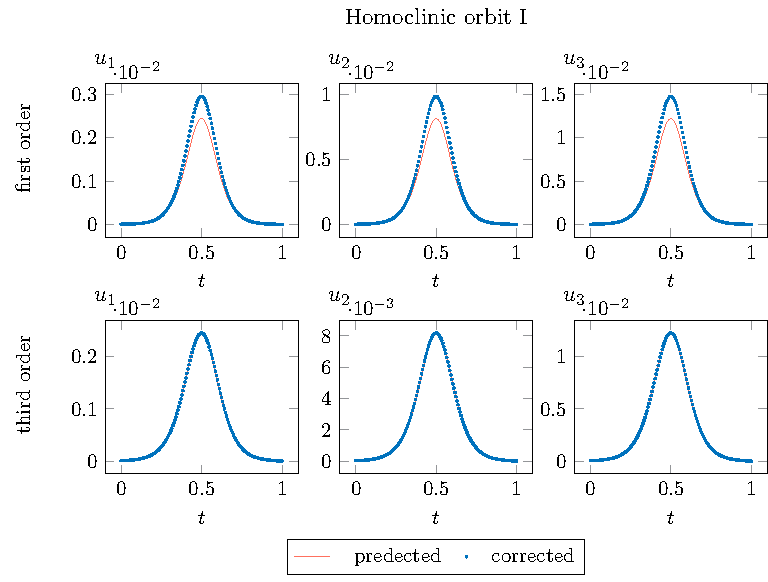
\includegraphics{\imagedir/TriNeuronBAMCompareProfilesI.pdf}
    \caption{Comparison between the first and third-order homoclinic asymptotics from
    \cref{btdde:sec:transcritical_bt_homoclinic_asymptotics} near the transcritical
        Bogdanov--Takens bifurcation in \cref{sm:eq:tri_neuron_BAM} with the
        perturbation parameter set to $\epsilon=0.02$.}
        \label{sm:fig:TriNeuronBAMCompareProfilesI}
\end{figure}

\begin{figure}[ht]
    \centering
    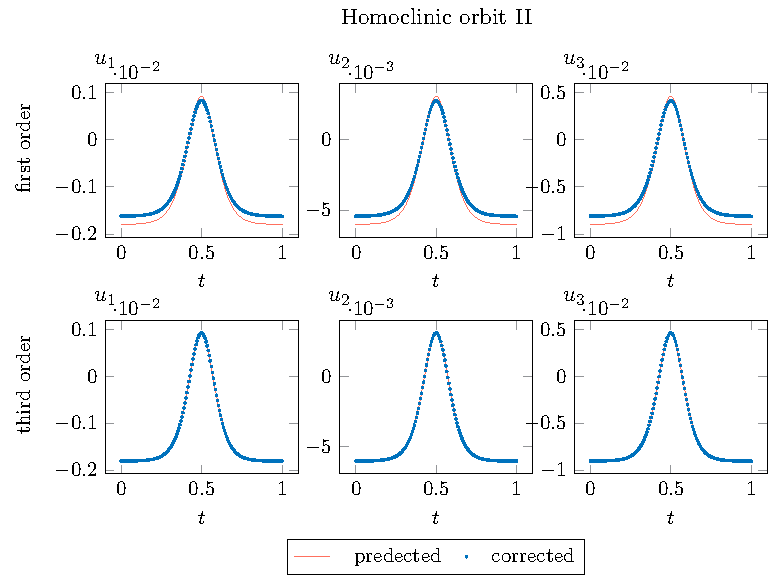
\includegraphics{\imagedir/TriNeuronBAMCompareProfilesII.pdf}
    \caption{Comparison between the first and third-order homoclinic asymptotics from
    \cref{btdde:sec:transcritical_bt_homoclinic_asymptotics} near the transcritical
        Bogdanov--Takens bifurcation in \cref{sm:eq:tri_neuron_BAM} with the
        perturbation parameter set to $\epsilon=0.02$.}
        \label{sm:fig:TriNeuronBAMCompareProfilesII}
\end{figure}

\subsection{Continuation of the codimension one curves emanating}
To continue the three codimension one curves emanating from the generic
Bogdanov--Takens we can simply use the function
\mintinline{MATLAB}{C1branch_from_C2point}, as show in the code below. To monitor the
continuation process the argument \mintinline{MATLAB}{plot} must be set \mintinline{MATLAB}{1}.
The most important setting is the perturbation parameter (or multiple),
\mintinline{MATLAB}{step} in the code below. If left out, default stepsizes are defined.
However, depending on the problem no convergence may then be obtained.
\inputminted[firstline=83, lastline=103]{MATLAB}{\pathToDDEBifToolDemos/BAM_neural_network_model/BAMnn.m}

\subsection{Predictors of the codimension one curves emanating from the Bogdanov--Takens point}
Before we provide the bifurcation diagram in the next section we first obtain the predictors
for the codimension one curves. For this we again use the function
\mintinline{MATLAB}{C1branch_from_C2point}. We set the argument \mintinline{MATLAB}{predictor} to \mintinline{MATLAB}{1}
and provide a range of perturbation parameters.
\inputminted[firstline=127, lastline=146]{MATLAB}{\pathToDDEBifToolDemos/BAM_neural_network_model/BAMnn.m}

\subsection{Bifurcation diagram}
The code below produce (a figure similar to) \cref{sm:fig:triNeuronBAMNeuralNetworkModelCompareParametersSupplementI}.
\inputminted[firstline=148, lastline=175]{MATLAB}{\pathToDDEBifToolDemos/BAM_neural_network_model/BAMnn.m}
%
\begin{figure}[ht]
\includetikzscaled{triNeuronBAMNeuralNetworkModelCompareParametersSupplementI}
\caption{Bifurcation diagram near the analytically derived transcritical
    Bogdanov--Takens point in \cref{sm:eq:tri_neuron_BAM} comparing the
    computed codimension one curves emanating form the Bogdanov--Takens piont
    using \DDEBIFTOOL with the third-order homoclinic parameter asymptotics
    obtained in \cref{btdde:sec:transcritical_bt_homoclinic_asymptotics}.}
\label{sm:fig:triNeuronBAMNeuralNetworkModelCompareParametersSupplementI}
\end{figure}

\subsection{Detect bifurcations on the second Hopf branch}
We can use the \DDEBIFTOOL function \mintinline{MATLAB}{LocateSpecialPoints} to
locate bifurcation points on the second Hopf banch.
\inputminted[firstline=177, lastline=178]{MATLAB}{\pathToDDEBifToolDemos/BAM_neural_network_model/BAMnn.m}

Inspecting the \MATLAB output gives.
\begin{minted}{shell-session}
HopfCodimension2: calculate stability if not yet present
HopfCodimension2: calculate L1 coefficients
HopfCodimension2: (provisional) 2 gen. Hopf 2 Takens-Bogdanov  detected.
br_insert: detected 1 of 4: genh. Normalform:
    L2: 5.7933e+03
    L1: 1.0106e-09

br_insert: detected 2 of 4: BT. Normalform:
    a2: -5.8499e-04
    b2: -0.0031

br_insert: detected 3 of 4: genh. Normalform:
    L2: -5.7933e+03
    L1: -2.1214e-09

br_insert: detected 4 of 4: BT. Normalform:
    a2: -0.0012
    b2: 0.0135
\end{minted}
Thus, there are two Bogdanov--Takens points detected. By inspection of the normal
form coefficients $a$ and $b$ (\mintinline{MATLAB}{a2} and
\mintinline{MATLAB}{b2} in the output above) with the coefficients of the
transcritical Bogdanov--Takens point we see that one is (very likely) already
known. Indeed, while continuing the second Hopf curve from the transcritical
Bogdanov--Takens point we encounter another Bogdanov--Takens point, at which
the Hopf curve turns around, and continues in the reverse direction, back to
the transcritical Bogdanov--Takens point. Similarly, we also deduce that there
is only one generalized Hopf point detected on the Hopf curve. Inspecting 
the parameters indeed confirm our claim.

Since the newly detect Bogdanov--Takens is detected on the Hopf curve
on which the equilbrium changes position under variation of the
parameters we extract the Bogdanov--Takens and computed the coefficients
of the generic case.
\inputminted[firstline=179, lastline=181]{MATLAB}{\pathToDDEBifToolDemos/BAM_neural_network_model/BAMnn.m}

\subsection{Plot Bogdanov-Takens test function along the Hopf curve}
Before we continu the homoclinic branch emanating from the generic
Bogdanov--Takens point we fist plot the testfunction for the Bogdanov--Takens
piont, i.e. we plot the imaginary part for the critical eigenvalues along the
second Hopf curve. The code below procedure (a figure similar to)
\cref{sm:fig:triNeuronBAMNeuralNetworkModelTestfunction}.
\inputminted[firstline=185, lastline=197]{MATLAB}{\pathToDDEBifToolDemos/BAM_neural_network_model/BAMnn.m}
%
\begin{figure}[ht]
    \centering
    \includetikzscaled{triNeuronBAMNeuralNetworkModelTestfunction}
    \caption{Plot of the Bogdanov--Takens testfunction along the second Hopf curve. 
    We see that surface $\omega=0$ is intersected transversally two times
    while continuing the Hopf curve.}
    \label{sm:fig:triNeuronBAMNeuralNetworkModelTestfunction}
\end{figure}

\subsection{Continue third homoclinic curve}
The code below continuous the homoclinic solution emanating from the generic Bogdanov--Takens detected
on the second Hopf branch. The last line extracts the parameters used for plotting.
\inputminted[firstline=199, lastline=205]{MATLAB}{\pathToDDEBifToolDemos/BAM_neural_network_model/BAMnn.m}

\subsection{Bifurcation plot}
We are now in the position to recreate the bifurcation plot as shown in the main paper. There we
left out the predictors for the codimension one equilbria bifurcation curves and changed the color
of the computed codimension one equilbria curvers to gray. In this way focus will be on
the homoclinic curvers. The code below procedure (a figure similar to)
\cref{sm:fig:triNeuronBAMNeuralNetworkModelCompareParameters}.
\inputminted[firstline=213, lastline=243]{MATLAB}{\pathToDDEBifToolDemos/BAM_neural_network_model/BAMnn.m}
\begin{figure}[ht]
    \includetikzscaled{triNeuronBAMNeuralNetworkModelCompareParameters}
    \caption{
    Bifurcation diagram near the transcritical Bogdanov--Takens bifurcation and
    a generic Bogdanov--Takens in \cref{sm:eq:tri_neuron_BAM-u} comparing computed
    codimension one curves using \DDEBIFTOOL with the asymptotics obtained in this
    paper.}
    \label{sm:fig:triNeuronBAMNeuralNetworkModelCompareParameters}
\end{figure}

\subsection{Large view bifurcation plot without predictors}
Although the first and third homoclinic bifurcation exists only in a very small
parameter region, the second is continued relatively large parameter range. The
code below produces (a figure similar to)
\cref{sm:fig:triNeuronBAMNeuralNetworkModelLargerBifurctionPlot}.
\inputminted[firstline=245, lastline=267]{MATLAB}{\pathToDDEBifToolDemos/BAM_neural_network_model/BAMnn.m}
\begin{figure}[ht]
    \includetikzscaled{triNeuronBAMNeuralNetworkModelLargerBifurctionPlot}
    \caption{
    Bifurcation diagram near the transcritical Bogdanov--Takens bifurcation and
    a generic Bogdanov--Takens in \cref{sm:eq:tri_neuron_BAM-u} showing the fully
    continued homoclinic branch connected to the non-trivial equilibrium emanating
    from the transcritical Bogdanov--Takens point.}
    \label{sm:fig:triNeuronBAMNeuralNetworkModelLargerBifurctionPlot}
\end{figure}

\subsection{Homoclinic orbits in phase-spase}
To obtain an expression of the continued homoclinic orbits in phase-space
we plot the solutions on the various homoclinic branches in phase-space.
The code below produces (a figure similar to)
\cref{sm:fig:triNeuronBAMNeuralNetworkModelOrbitsPhaseSpace}.
In the top left plot the homoclinic orbits connected to the origin are show. However,
we see that this doesn't provide much insight. 
One way to visualize homoclinic solution is by inspection the
profiles of the solution. This we will be done in the next section.
Another way is reveal the homoclinic solutions connected to the origin is by
rotating the coordinates $(u_1,u_2)$. The result is seen in the top right
plot in \cref{sm:fig:triNeuronBAMNeuralNetworkModelOrbitsPhaseSpace}.
In the bottom left plot the solutions on the second homoclinic branch emanating
from the transcritical Bogdanov--Takens point are shown. Lastly, we plotted the
rotated homoclinic homoclinic orbits emanating from the generic
Bogdanov--Takens point in the bottom right plot of
\cref{sm:fig:triNeuronBAMNeuralNetworkModelCompareOrbitsPhaseSpace}.
\inputminted[firstline=269, lastline=335]{MATLAB}{\pathToDDEBifToolDemos/BAM_neural_network_model/BAMnn.m}
\begin{figure}[ht]
    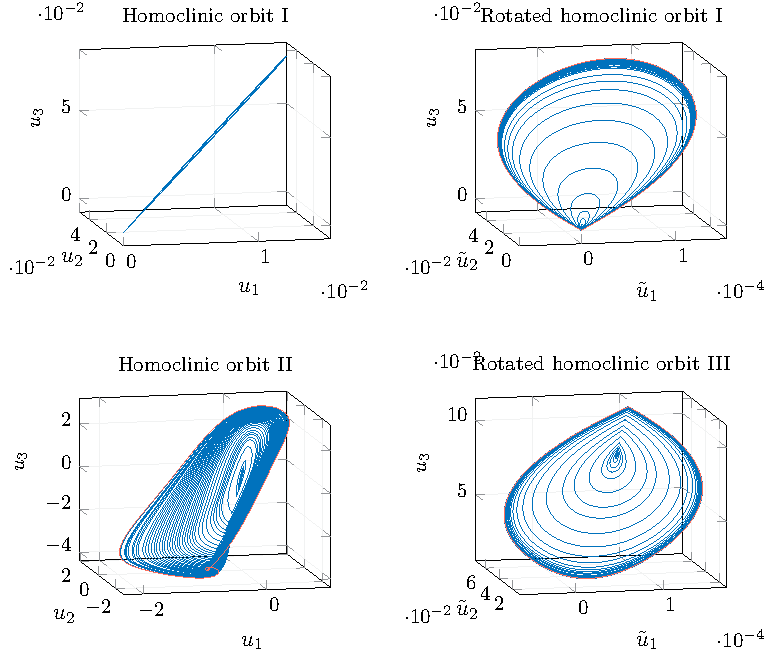
\includegraphics[width=\textwidth]{\imagedir/triNeuronBAMNeuralNetworkModelOrbitsPhaseSpace.pdf}
    \caption{
    Plots of homoclinic solutions emanating from the generic and transcritical
    Bogdanov--Takens bifurcations in \cref{sm:eq:tri_neuron_BAM-u}. In the top
    left plot the homoclinic solutions emanating from the transcritical
    Bogdanov--Takens point with fixed saddle points a shown. In the top right
    plot we rotated the $(u_1, u_2)$ coordinates in order to make these
    homoclinic solutions visible. The bottom left plot shows the second branch
    of homoclinic solutions emanating from the transcritical Bogdanov--Takens
    point. Lastly, in the bottom right plot the homoclinic solutions emanating
    from the generic Bogdanov--Takens point are shown. Here also the $(u_1,
    u_2)$ coordinates are rotated.
    }
    \label{sm:fig:triNeuronBAMNeuralNetworkModelOrbitsPhaseSpace}
\end{figure}


\subsection{Compare homoclinic solutions in phase-space}
Here we compare the correct and uncorrected profiles of the homoclinic
solutions on the two homoclinic curves emanating from the transcritical
Bogdanov--Takens point with the perturbation parameter ranging from $0.003$ to
$0.009$.
The code below produce (a figure similar to)
\cref{sm:fig:triNeuronBAMNeuralNetworkModelCompareOrbitsPhaseSpace}. We see
that the corrected and predicted homoclinic orbits are nearly identical.
\inputminted[firstline=356, lastline=385]{MATLAB}{\pathToDDEBifToolDemos/BAM_neural_network_model/BAMnn.m}
%
\begin{figure}[ht]
    \includetikzscaled{triNeuronBAMNeuralNetworkModelCompareOrbitsPhaseSpace}
    \caption{Plot comparing the third-order homoclinic asymptotics with the
        Newton correct homoclinic solutions in $(\epsilon,\tilde t, u_1)$
        phase-space. Here $\tilde t$ is the time $t$ rescaled to the interval
        $[0,1]$.
    }
    \label{sm:fig:triNeuronBAMNeuralNetworkModelCompareOrbitsPhaseSpace}
\end{figure}

\subsection{Continue periodic solutions from Hopf branch to homoclinic branch}
We continue a branch of periodic solutions emanating from point number 29 on the
first Hopf branch emanating from the transcritical Bogdanov--Takens point. The
periodic solution convergence to a homoclinic orbit located on the second
homoclinic branch emanating from transcritical Bogdanov--Takens point. We will
use point number 28 on the periodic solution branch to compare against the
simulation in Julia in \cref{sm:sec:triNeuralBAMNetworkModelSimulation}. The
code below produces (a figure similar to)
\cref{sm:fig:triNeuronBAMNeuralNetworkModelPeriodicSolutions}.
\inputminted[firstline=387, lastline=391]{MATLAB}{\pathToDDEBifToolDemos/BAM_neural_network_model/BAMnn.m}
\vspace*{-12pt}
\inputminted[firstline=398, lastline=414]{MATLAB}{\pathToDDEBifToolDemos/BAM_neural_network_model/BAMnn.m}
\begin{figure}[ht]
    \includetikzscaled{triNeuronBAMNeuralNetworkModelPeriodicSolutions}
    \caption{
        Branch of periodic solutions emanating from the last point on the first
        Hopf branch emanating from the transcritical Bogdanov--Takens point in
        \cref{sm:eq:tri_neuron_BAM-u}. The last point on the perioidic solution
        branch is colored red, at which the periodic orbits have converged to
        a homoclinic orbit.
    }
    \label{sm:fig:triNeuronBAMNeuralNetworkModelPeriodicSolutions}
\end{figure}

\subsection{\ifthesis \phantom{ } \fi Homoclinic branch connecting the two Bogdanov--Takens \ifthesis \phantom{ } \fi points}
Here we will show that the transcritical Bogdanov--Takens and generic
Bogdanov--Takens points are connected, not only by a Hopf curve, but also
through a homoclinic curve. For this we first, we again continue the 
second Hopf branch emanating from the transcritical Bogdanov--Takens point,
but with a smaller step-size.
\inputminted[firstline=416, lastline=429]{MATLAB}{\pathToDDEBifToolDemos/BAM_neural_network_model/BAMnn.m}
%
Next, we continue from (almost) each point on the new Hopf branch the emerging periodic solutions.
\inputminted[firstline=436, lastline=446]{MATLAB}{\pathToDDEBifToolDemos/BAM_neural_network_model/BAMnn.m}
%
By plotting the last point on each of the periodic solutions branches in
$(\alpha_1, \tilde u_1, \tilde u_2)$-space,
together with the homoclinic solutions on the first and third homoclinic branches continued
above, it is indeed clear that the two homoclinic branches are connected through a
single homoclinic curve, see
\cref{sm:fig:triNeuronBAMNeuralNetworkModelConnectionHomoclinicSolutions}.
We also see how the transition is made from the homoclinic orbits with a fixed saddle point
at the origin to the homoclinic orbits with a moving saddle. Clearly, \DDEBIFTOOL has
difficulties continuing the homoclinic orbits near the gloal homoclinic bifurcation point.
\inputminted[firstline=461, lastline=490]{MATLAB}{\pathToDDEBifToolDemos/BAM_neural_network_model/BAMnn.m}
%
\begin{figure}[ht]
    \includetikzscaled{triNeuronBAMNeuralNetworkModelConnectionHomoclinicSolutions}
    \caption{
        Branch of homoclinic solutions (orange) connecting the transcritical Bogdanov--Takens point (the right black dot) with
        the generic Bogdanov--Takens point (the left black dot) in
        \cref{sm:eq:tri_neuron_BAM-u}. The blue homoclinic curve emerging from 
        the transcritical and generic Bogdanov--Takens points are the previously continued
        homoclinic branches.
     }
    \label{sm:fig:triNeuronBAMNeuralNetworkModelConnectionHomoclinicSolutions}
\end{figure}
To obtain an impression of the parameter curves connecting the transcritical Bogdanov--Takens and
generic Bogdanov--Takens points, we rotated the  curves through an angle of $\theta_2=0.646045233034992$.
By doing so, the two Bogdanov--Takens points are aligned on the abscissa. In
\cref{sm:fig:triNeuronBAMNeuralNetworkModelConnectionHomoclinicParameters} we plotted the first and third homoclinic branch, emanating from the
transcritical Bogdanov--Takens and generic Bogdanov--Takens points
respectively, the Hopf curve connecting the two Bogdanov--Takens points, and
the newly obtained homoclinic bifurcation curve.
\inputminted[firstline=501, lastline=529]{MATLAB}{\pathToDDEBifToolDemos/BAM_neural_network_model/BAMnn.m}
\begin{figure}[ht]
    \centering
    \includetikzscaled{triNeuronBAMNeuralNetworkModelConnectionHomoclinicParameters}
    \caption{
    Bifurcation diagram near the transcritical Bogdanov--Takens bifurcation and
    a generic Bogdanov--Takens in \cref{sm:eq:tri_neuron_BAM-u} showing the fully
    continued homoclinic branch connected to the non-trivial equilibrium emanating
    from the transcritical Bogdanov--Takens point.}
    \label{sm:fig:triNeuronBAMNeuralNetworkModelConnectionHomoclinicParameters}
\end{figure}


\subsection{Convergence plot}
\label{sm:sec:tri_neuron_BAM:convergence_plot}
Using the function from \cref{sm:lst:convergence_plot} we create a log-log
convergence plot comparing the convergence order of the first and thrid order
homoclinic asymptotics from \cref{btdde:sec:transcritical_bt_homoclinic_asymptotics}.
The code below yields \cref{sm:fig:triNeuralBAMNetworkModelConvergencePlot}.
\inputminted[firstline=531, lastline=542]{MATLAB}{\pathToDDEBifToolDemos/BAM_neural_network_model/BAMnn.m}
\begin{figure}[ht]
    \centering
    \includetikz{triNeuralBAMNetworkModelConvergencePlot}
     \caption{On the abscissa is the approximation to the amplitude $A_0$ and on
        the ordinate the relative error $\delta$ between the constructed solution
        \mintinline{MATLAB}{hcli_pred} to the defining system for the homoclinic orbit
        and the Newton corrected solution \mintinline{MATLAB}{hcli_corrected}.}
    \label{sm:fig:triNeuralBAMNetworkModelConvergencePlot}
\end{figure}

\subsection{Simulation with {\tt DifferentialEquations.jl}}
\label{sm:sec:triNeuralBAMNetworkModelSimulation}
Here we will preform four simulations. The first two simulations will be at two
homoclinic orbits located on the two homoclinic curves emanating from the
transcritical Bogdanov--Takens point continued with \DDEBIFTOOL, see
\cref{sm:fig:triNeuralBAMNetworkSimulationHomoclinic}. The second two simulations will be in
the regions where there should be stable periodic orbits, see
\cref{sm:fig:triNeuralBAMNetworkSimulationPeriodic}.

\begin{figure}[ht]
    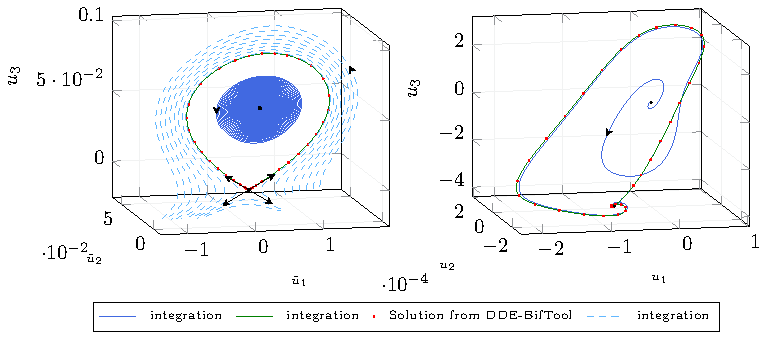
\includegraphics{\imagedir/triNeuralBAMNetworkModelHomoclinicSimulation.pdf}
    \caption{Comparing the computed homoclinic orbits in \cref{sm:eq:tri_neuron_BAM-u}
    with \DDEBIFTOOL with the solutions obtain from numerical simulation with Julia.
    We see the numerical integrated solution
    going through all the red points from the solution from \DDEBIFTOOL.}
    \label{sm:fig:triNeuralBAMNetworkSimulationHomoclinic}
\end{figure}

\begin{figure}[ht]
    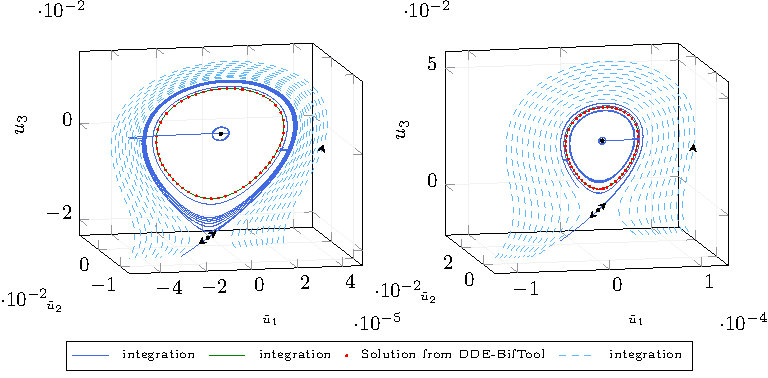
\includegraphics{\imagedir/triNeuralBAMNetworkModelPeriodicSimulation.pdf}
    \caption{Comparing the computed periodic orbits in \cref{sm:eq:tri_neuron_BAM-u}
    with \DDEBIFTOOL with the solution obtain from numerical simulation with Julia.
    We see the numerical integrated solution
    going through all the red points from the solution from \DDEBIFTOOL.}
    \label{sm:fig:triNeuralBAMNetworkSimulationPeriodic}
\end{figure}

\subsubsection{Loading necessary Julia packages}
We start by loading the necessary Julia packages. Compared with the preivious
demonstrations we also need to load the Julia package {\tt Symbolics.jl} to
differentiate the activation functions $f_1,f_2,f_3$.
\inputminted[firstline=1, lastline=9]{julia}{\pathToJuliaFiles/triNeuralBAMNetworkModel_simulation_article.jl}

\subsubsection{Define system}
Next we define the system to be integrated, a system to approximate the reverse
flow, and also a allocating version used for stability calculations. Note there
we need the Julia {\tt Symbolics.jl} to differentiate the activation functions.
\inputminted[firstline=11, lastline=63]{julia}{\pathToJuliaFiles/triNeuralBAMNetworkModel_simulation_article.jl}

\subsubsection{Function for creating streamlines plot}
To obtain an impression of the flow near transcritical Bogdanov--Takens point
we create a streamlines function. This is particularly useful for seeing the
flow around the stable manifold of the saddle-note.
\inputminted[firstline=65, lastline=77]{julia}{\pathToJuliaFiles/triNeuralBAMNetworkModel_simulation_article.jl}

\subsubsection{Create figure with several axes}
We create a figure containing multiple axis in which we will plot 
the homoclinic, periodic orbits, and the left and right-hand sides
of \cref{sm:eq:triNeuralBAMNetworkModel:tan}.
\inputminted[firstline=79, lastline=89]{julia}{\pathToJuliaFiles/triNeuralBAMNetworkModel_simulation_article.jl}

\subsubsection{Define parameters, equilbria}
We define parameters located on the continued homoclinic branch with
\DDEBIFTOOL. Then calculate the equilbria points in \cref{sm:eq:tri_neuron_BAM}
near the transcritical Bogdanov--Takens point.
\inputminted[firstline=91, lastline=98]{julia}{\pathToJuliaFiles/triNeuralBAMNetworkModel_simulation_article.jl}

\subsubsection{Plot equilbria and homoclinic orbit}
By plotting the homoclinic orbit obtained with \DDEBIFTOOL located at parameter
values $(\alpha_1, \alpha_2) = (-0.001724521613831, 0.001344362436730)$ we can
compare with the numerical simulations. As in the analysis with \DDEBIFTOOL, we
rotate the coordinates of the solutions to visualize the solutions in
phase-space.
\inputminted[firstline=100, lastline=110]{julia}{\pathToJuliaFiles/triNeuralBAMNetworkModel_simulation_article.jl}

\subsubsection{Leading eigenvectors}
Next, we calculate and plot the leading eigenvectors of the characteristic matrix at the saddle-node bifurcation point.
\inputminted[firstline=112, lastline=135]{julia}{\pathToJuliaFiles/triNeuralBAMNetworkModel_simulation_article.jl}

\subsubsection{Define callback}
Since we are only interested in the flow near the equilbria points we create a
continuous callback to ensure the orbits don't become the large.
\inputminted[firstline=137, lastline=140]{julia}{\pathToJuliaFiles/triNeuralBAMNetworkModel_simulation_article.jl}

\subsubsection{Integrate the system at homoclinic orbits I}
Now we define the problem to be integrated and choose the algorithm to be used.
Then we integrate the system for a range of initial history functions using the
function \mintinline{julia}{streamlines}. Next, we integrate the system near
the inner equilibrium, i.e., the equilibrium inside the homoclinic orbit. This
equilibria should be an unstable spiral. We show the first and last part
of the obtained solution. We see that the last part of the integrated solutions
completely overlaps the homoclinic solution obtained with \DDEBIFTOOL.
\inputminted[firstline=142, lastline=165]{julia}{\pathToJuliaFiles/triNeuralBAMNetworkModel_simulation_article.jl}

\subsubsection{Add arrows on solutions}
Lastly, we add arrows to the obtained solutions and redraw the equilbria.
\inputminted[firstline=167, lastline=178]{julia}{\pathToJuliaFiles/triNeuralBAMNetworkModel_simulation_article.jl}
We should now obtain an interactive figure similar to the left figure in
\cref{sm:fig:triNeuralBAMNetworkSimulationHomoclinic}.

\subsubsection{Simulation near stable periodic orbit I}
The code for numerical simulation near the second homoclinic orbit, see the
right plot in \cref{sm:fig:triNeuralBAMNetworkSimulationHomoclinic}, is not
included here.

To show by integration the existence of an stable periodic orbit we first
located a periodic orbit in \DDEBIFTOOL. This can be done by continuing a
branch of periodic orbits emanating from a point on the continued Hopf curves.
Then we load the profiles of the periodic orbits into Julia. We preform
two simulations. The first starts integrating with a constant history function
equal inside the periodic orbit. The second starts from the unstable eigenvector
of the characteristic matrix calculated above.
\inputminted[firstline=237, lastline=328]{julia}{\pathToJuliaFiles/triNeuralBAMNetworkModel_simulation_article.jl}
After running the above code we should obtain a similar plot as in
\cref{sm:fig:triNeuralBAMNetworkSimulationPeriodic}.

\subsubsection{Stability of the center manifold}
To confirm \cref{sm:lemma:triNeuralBAMNetworkModelEigenvalues} nummerically we
consider again
\cref{sm:eq:triNeuralBAMNetworkModelFunctions,sm:eq:triNeuralBAMNetworkModelFixedParameters}.
The code below plots the left and right-hand sides of
\cref{sm:eq:triNeuralBAMNetworkModel:tan}. We see in
\cref{sm:fig:triNeuralBAMNetworkStabilityDeterminingFunction} that there are
two point of intersection.
\inputminted[firstline=421, lastline=439]{julia}{\pathToJuliaFiles/triNeuralBAMNetworkModel_simulation_article.jl}
\begin{figure}[ht]
    \centering
    \includetikzscaled{triNeuralBAMNetworkModelStabilityDeterminingFunction}
    \caption{Plot of the left and right-hand sides of
    \cref{sm:eq:triNeuralBAMNetworkModel:tan}. Points of intersection are
    canditates for the center manifold to lose its stability.}
    \label{sm:fig:triNeuralBAMNetworkStabilityDeterminingFunction}
\end{figure}
Using the function \mintinline{julia}{roots} from the package {\tt IntervalRootFinding.jl}
we search for points of intersection. 
\inputminted[firstline=441, lastline=444]{julia}{\pathToJuliaFiles/triNeuralBAMNetworkModel_simulation_article.jl}
In the Julia output we obtain
\begin{minted}{shell-session}
7-element Vector{Root{Interval{Float64}}}:
 Root([13.2309, 13.231], :unique)
 Root([19.2374, 19.2375], :unique)
 Root([19.7337, 19.7338], :unknown)
 Root([6.00301, 6.00302], :unique)
 Root([8.33333, 8.33334], :unknown)
 Root([13.5353, 13.5354], :unknown)
 Root([5.75402, 5.75403], :unknown)
 Root([8.33333, 8.33334], :unknown)
\end{minted}
Note that, since there are multiple discontinuities, there are many unknown
solutions given. We extract the unique solutions from the list of solutions
and test if these provide solutions to the characteristic equation.
\inputminted[firstline=446, lastline=457]{julia}{\pathToJuliaFiles/triNeuralBAMNetworkModel_simulation_article.jl}
In the Julia output we obtain
\begin{minted}{shell-session}
The centermanifold is locally attractive for 0 < τ < 13.230934887939895.
\end{minted}

\begin{figure}[ht]
    \centering
    \includetikzscaled{triNeuralBAMNetworkModelEigenvalues}
    \caption{Plot of the leading eigenvalues at the analytically derived
    transcritical Bogdanov--Takens point with $\tau = 13.230934887939895$
    and $\omega = \omega(\tau)$ from \cref{sm:eq:BAM_omega}. At this
    point there are four eigenvalues on the imaginary axis. For
    $\tau > 13.230934887939895$ the center manifold is locally unstable.}
    \label{sm:fig:triNeuralBAMNetworkModelEigenvalues}
\end{figure}
\subsubsection{Calculate and plot stability at Bogdanov--Takens point}
We fininsh this demonstration by confirming the stability
of the transcritical Bogdanov--Takens points at $\tau = 13.230934887939895$
obtained in the previous section. In \cref{sm:fig:triNeuralBAMNetworkModelEigenvalues}
we have plotted the eigenvalues. We indeed see that at $\tau = 13.230934887939895$
the center manifold looses stability. Lastly, we also varified in the code
below that the the eiganvalues with positive imaginary part on the imaginary axis
is approximatly equal to the expression for $\omega$ obtained in \cref{sm:eq:BAM_omega}. 
\inputminted[firstline=459, lastline=467]{julia}{\pathToJuliaFiles/triNeuralBAMNetworkModel_simulation_article.jl}



%% CHAOS Paper
\tikzsetexternalprefix{./images/chaoticRGflow/} 
\renewcommand\tikzdir{./tikz/chaoticRGflow}
\renewcommand\imagedir{./images/chaoticRGflow/}
\renewcommand\datadir{./data/chaoticRGflow}
\chapter{Chaotic RG Flow in Non-Unitary Tensor Models}
\label{chapter:chaoticRGFlow}
\paragraph{{\color{header1}Abstract}}We study bi-antisymmetric tensor quantum field theories with $O(N_1)\times O(N_2)$ symmetry. Working in $4-\epsilon$ dimensions we calculate the beta functions up to second order in the coupling constants and analyze in detail the Renormalization Group (RG) flow and its fixed points. We allow $N_1$ and $N_2$ to assume general real values and treat them as bifurcation parameters. In studying the behavior of these theories in a non-unitary regime in the space of $N_1$ and $N_2$ we find a point where a zero-Hopf bifurcation occurs. In the vicinity of this point, we provide analytical and numerical evidence for the existence of Shilnikov homoclinic orbits, which induce chaotic behavior in the RG flow of a subset of nearby theories. As a simple warm-up example for the study of chaotic RG flows, we also review the non-hermitian Ising chain and show how for special complex values of the coupling constant, its RG transformations are equivalent to the Bernoulli map\footnote{Published as
\bibentry{PhysRevD.105.065021}}.

\section{Introduction}

Science abounds with examples of systems governed by simple rules yet exhibiting marvelously complex behaviors. A broad class of instances of this phenomenon is the occurrence of chaos in dynamical systems. By a dynamical system, we mean a system of autonomous first-order differential equations or discrete maps:
\begin{gather}
\dot{g}_i = \beta_i(g_j)\,, \hspace{20mm} g_i^{(n+1)} = \mathcal{R}_i\left(g_j^{(n)}\right)\,, \label{eq:dynsys}
\end{gather}
where the variables $g_i$ are either real- or complex-valued. The study of chaos in such systems dates back to the work of Henri Poincar\'e\ on the three-body problem. In the Hamiltonian formalism, the trajectories of particles in phase space are described precisely by the kind of first-order differential equations listed in \cref{eq:dynsys}. In his investigation of the three-body equations of motion, Poincar\'e\ was startled to discover that the solution space is vastly more intricate than he had anticipated, encompassing meandering curves of ever-increasing wiggles and an infinitude of periodic orbits dispersed unevenly in phase space. Since the time when Poincar\'e\ caught his first glimpse of chaos, the characteristic properties by which one can identify chaos have become much better understood. In addition to the presence of an infinite number of periodic orbits with an infinite range of periodicities, sometimes forming complicated fractal structures, chaotic systems are characterized by an extreme sensitivity to initial conditions as well as by the property that open sets of initial states evolve in time to spread out densely in the space of all possible states. For a more detailed discussion of what is meant by the term chaos, we refer the reader to \cref{appendix:chaos}.


Dynamical systems have a wide range of applications in science and technology, and the emergence of chaos is a commonplace occurrence in these applications, be they planetary orbits, atmospheric convection \cite{lorenz1963deterministic}, string theory \cite{maldacena2016remarks,Gross:2021gsj,PhysRevLett.127.021601} or population dynamics \cite{Arnold_1983}. In modern theoretical physics, an important class of dynamical systems are furnished by the beta functions of quantum field theories (QFTs) and their associated \textit{renormalization group (RG) flows}. Rather than trajectories of particles in phase space, these systems describe the flow of coupling constants in a given theory as we vary the length or energy scale at which we view the theory, but the flow equations remain of the form \cref{eq:dynsys}.  Consequently, in their most general form, QFTs should admit chaotic RG flows, and already Wilson and Kogut entertained this possibility in their classic review \cite{Wilson:1973jj}. However, the theories typically studied by physicists exclusively exhibit an RG flow of a simpler kind, namely heteroclinic flow between fixed points.  Associated herewith is the idea of universality: we can modify the details of the high-energy (UV) theory and still flow to the same low-energy (IR) theory if we remain in the same basin of attraction. Contrariwise, chaos would spell the doom of universality, with even the tiniest change to the UV theory drastically altering the IR theory. In two, three, and four dimensions it is known that unitarity prevents this kind of behavior by guaranteeing the existence of $c$-, $F$-, or $a$-functions that change monotonically under RG flow \cite{zamolodchikov1986irreversibility,Klebanov:2011gs,Jafferis:2011zi,Casini:2012ei,Komargodski:2011vj,Luty:2012ww}, and the same may be true in higher dimensions. It has further been suggested \cite{Binder:2019zqc} that universality may extend beyond the realm of unitary theories. Nevertheless, the 80s and 90s bore witness to a number of ideas for and examples of chaotic RG flows in certain simple systems \cite{mckay1982spin,berker1984hierarchical,svrakic1982hierarchical,Damgaard:1991zh, Damgaard:1991zb, Dolan:1994wt}, see also \cite{Damgaard:1991zb} for a general discussion. In all these examples, the RG transformations are discrete. The realization of chaos here hinges on the underlying model being non-unitary or involving an unusual hierarchical coupling pattern of spins with no conventional continuum limit, or the chaos arises as an artifact of discrete and approximate RG transformations, in the same manner as the logistic map is chaotic while the solution to the logistic differential equation is monotonic. 

In the present paper, we present a family of QFTs of which a subset of non-unitary theories exhibit continuous RG flows that are chaotic. The models arise on analytic continuation of conventional theories by allowing symmetry groups of matrices of non-integer size. The specific models have no concrete experimental motivation and are intended rather to serve as a proof of principle, but non-unitary theories generally, as well as theories with symmetry groups of non-integer size specifically, are capable of describing physical phenomena that can be realized experimentally. The list of non-unitary models of interest in theoretical physics includes such theories as the $q$ state Potts model with $q>4$ \cite{1982RvMP...54..235W,gorbenko2018walking,Gorbenko:2018dtm}, logarithmic CFTs \cite{Gurarie:1993xq,cardy2013logarithmic}, and Liouville theory in dimensions greater than 2 \cite{levy2018liouville}. Furthermore, we observe that analytical continuation of RG flows of conventional field theories provides a method of generating a vast range of dynamical systems. This suggests the possibility of studying systems of interest outside of theoretical physics using QFT methods. As a point in case, we demonstrate in the next section that the Bernoulli map is secretly identical to the RG transformations of the 1d Ising model at special complex values of the coupling constant.

In general, it is very difficult to conclusively prove the presence of chaos in a system, but some tools are available. One method is to map a system onto one of the few well-studied systems that are known to be chaotic. We apply this method in \cref{sec:Ising}, where, as a toy model with chaotic behavior, we analyze the complexified Ising chain, which was previously studied and shown to be chaotic in \cite{Dolan:1994wt}. For continuous dynamics, a set of necessary conditions for the onset of chaotic dynamics, involving the presence of a homoclinic orbit, was put forward by Shilnikov \cite{shilnikov1965case}. We review his construction in \cref{sec:Shilnikov}. Subsequent to Shilnikov's discovery, mathematicians were able to show that for two-parameter families of dynamical systems, in the vicinity of a certain kind of bifurcation there will generically exist a subset of systems that satisfy Shilnikov's conditions \cite{baldoma2020hopf}. In \cref{sec:QFT}, we present a family of tensor models with $O(N_1)\times O(N_2)$ symmetry whose beta functions undergo such a bifurcation at the special values $N^\ast_1=2.521$, $N^\ast_2=1.972$, and we provide numerical evidence that there exist Shilnikov homoclinic orbits among the RG trajectories of a codimension one subset of models with $(N_1,N_2)$ close to $(N^\ast_1,N^\ast_2)$. Thereby we establish that these QFTs exhibit chaotic RG flow.



\section{The Complex Ising Chain and the Bernoulli Map}
\label{sec:Ising}
In this section, as an illustration of the ideas of chaos discussed in the introduction and as an example of how universality extends beyond unitarity but breaks down in special chaotic regions, we will consider the one-dimensional Ising model with a complex coupling. This model and its chaotic behavior was also studied in \cite{Dolan:1994wt}. Once coupling constants in a theory are complex, all sorts of RG flows become possible. For instance, it is quite easy to find limit cycles \cite{faedo2021multiple}. The consideration of complex RG fixed points was previously proposed in \cite{Gorbenko:2018dtm,Gorbenko:2018ncu} and further carried out in the context of tensor models in \cite{Giombi:2017dtl}.  The complex Ising model in this section serves as a warm-up for the more intricate model in \cref{sec:QFT}, where we will realize chaos in the RG flow of real-valued coupling constants.



In the absence of an external magnetic field, the Hamiltonian of the one-dimensional Ising model is given by
\begin{gather}
  H = g \sum_i \sigma_i \sigma_{i+1}\,,
\end{gather}
where $i$ runs over some set of integer labels, and the spin variables $\{\sigma_i\}$ can assume the values $\pm 1$. The  1$d$ Ising model has been studied extensively in the literature, and there are numerous methods to solve it numerically and analytically. The system does not exhibit a phase transition, and we can compute the correlation functions exactly. The most common method of solving the model involves the use of a transfer matrix, which can also be used to implement the RG flow of the model. The idea is the following: the partition function is given by
\begin{gather}
 Z = \sum_{ \left\{ \sigma_i = \pm 1\right\}} \prod_i C e^{-g \sigma_i \sigma_{i+1}}\,,
 \label{Z}
\end{gather}
where we allow for a normalization constant $C$. Supposing we have $N$ spin variables $\sigma_i$ and impose periodic boundary conditions $\sigma_i=\sigma_{N+i}\,$, we notice that we can introduce a matrix $T$ such that
\begin{gather}
T = C\begin{pmatrix}
 e^{-g} & e^{g}\\
 e^{g} & e^{-g}
\end{pmatrix},\hspace{20mm} Z  = \operatorname{tr}\left[ T^N\right] \,. \label{eq:partfunc}
\end{gather}
Now let us carry out one step of an RG flow by integrating out some degrees of freedom of the model, for example the spins with odd indexes in the chain. It is possible to express the partition function in terms of the remaining degrees of freedom by an equation still of the form \cref{Z}, except that the coupling constant $g$ has to be replaced by a different coupling constant $g_1$, and $C$ by a new normalization constant $C_1$: 
\begin{gather}
 Z = \sum_{ \left\{ \sigma_i = \pm 1\right\}} \prod_{i \text{ even}} C_1e^{-g_1 \sigma_i \sigma_{i+1}}\,.
 \label{Z1}
\end{gather}
The new constants $g_1$ and $C_1$ can be computed by noticing that integrating out the odd spins formally leads to the replacement $T\to T^2 \equiv T_1$. Demanding that $T_1$ has the same form as the original transfer matrix $T$ gives the equation:
\begin{gather}
C^2\begin{pmatrix}
  e^{-2g}+e^{2g} & 2\\
  2 & e^{-2g}+e^{2g}
\end{pmatrix}
=
C_1\begin{pmatrix}
 e^{-g_1} & e^{g_1}\\
 e^{g_1} & e^{-g_1}
\end{pmatrix}
\,.
\end{gather}
This equation implies that the RG step relates the old coupling $g$ to the new coupling $g_1$ via the relation
\begin{gather}
  e^{-2g_1} =\frac{(T^2)_{11}}{(T^2)_{12}}=\frac12\left(e^{-2g}+e^{2g} \right) = \cosh 2g\,.
\end{gather}
For convenience we introduce a new parameter $z=e^{-2g}$, in terms of which the RG step assumes the simple form
\begin{gather}
 z_1 = \frac12\left(z + \frac{1}{z}\right)  \equiv R(z)\,.
\end{gather}
Let us first consider the unitary Ising model, which means we take $z$ to be real and positive. In this case, the sequence
$z_n = R(z_{n-1})$
is convergent. To see this, note that for any positive real, $z$ we have that $z_1 = \frac12\left(z+\frac{1}{z}\right) \geq 1$.
Furthermore, for any $z_n>1$, we have that $z_{n+1} = R(z_n) \leq \frac{1}{2}\left(z_n+1\right) < z_n$. Hence, the sequence $z_1$,$z_2$,$z_3$,$\ldots$ is decreasing, and since it is also bounded below, it is convergent. 
The fixed point that the sequence converges to is situated at $z=1$, i.e. $g=0$, corresponding to a high temperature fixed point.

Suppose now that we do not constrain ourselves to unitary theories and allow $g$ and $z$ to assume complex values. By an argument analogous to the above, one can show that as long as $\operatorname{Re} z \neq 0$, the sequence remains convergent, converging to the value $\operatorname{sign}(z)$. However, as we will now demonstrate, when $z$ is imaginary, the behavior of the sequence changes drastically and chaos emerges. It is not hard to see that when $z_n\equiv i x_n$ is imaginary, then $\widetilde{R}(i x_n)\equiv ix_{n+1}$ is also imaginary, and we have
\begin{gather}
x_{n+1} = \tilde{R}(x_{n})\,,\hspace{20mm} \widetilde{R}(x) \equiv \frac12\left(x-\frac{1}{x}\right)\,.
\end{gather}
We now introduce a parameter $t_n \in \left[0,1\right)$ related to $x_n$ via the equation $x_n = \tan \big(\pi(t_n-\frac12)\big)$. Then the RG step acts on $t_n$ as
\begin{gather}
t_{n+1} = 2 t_n \mod 1\,. \label{tRG}
\end{gather}
This map is known as the dyadic map or the Bernoulli map and was introduced %in 1957
by R\'enyi \cite{renyi1957representations} as part of a larger class of transformations that he proved to be ergodic. Despite the simplicity of the map, it exhibits all the characteristics of chaotic flow. One immediate observation is that the map has a non-zero Lyapunov exponent: $\delta t_{n+k} = 2^k \delta t_n$ for sufficiently small $\delta t_n$, although this behavior breaks down at large values of $k$ since $t$ is constrained to a finite interval. It is also not hard to see that for any finite interval $I \subset [0,1]$ of initial values of $t_0$, the image of $I$ under repeated RG steps will eventually spread out over the whole interval $[0,1]$. Furthermore, suppose we decompose the starting value $t_0$ of $t$ in a binary expansion:
\begin{gather}
t_0=\sum_{i=1}^\infty a_i\,2^{-i}\,, 
\end{gather}
where $a_i \in \{0,1\}$. The semi-infinite sequence $A=\left\{a_i\right\}^\infty_{i=1}$ provides all information concerning the initial state and subsequent evolution of the system. And the application of an RG step \cref{tRG} corresponds to discarding $a_1$ and shifting $a_{i+1} \to a_{i}$. From this point of view, we can exactly predict the evolution of the system when the initial state is known exactly, but any variation whatsoever of the initial state will eventually lead to the largest possible fluctuations in future values of the state of the system. Thus, if $t_0 \in \mathbb{Q}$, the sequence $A$ will be periodic after a finite number of initial digits, meaning that the RG flow becomes cyclic. More precisely, we can express any $t_0 \in \mathbb{Q}$ as a reduced fraction $t_0 = 2^m\frac{q}{r}$ where $m,q\in \mathbb{Z}$, $r\in\mathbb{N}$, and gcd$(q,r)=$gcd$(q,2)=$gcd$(r,2)=1$, in which case the periodicity of the RG flow is simply $r$, while max$(-m,0)$ equals the number of initial digits in $A$ before the sequence becomes periodic. From the above it follows that all periodicities are realized for some initial values of $t$ and that any finite interval of initial values induces RG flows with an infinite set of different periods. Meanwhile, if $t_0 \notin \mathbb{Q}$, then the sequence $A$ does not have a limit cycle. Moreover, one can show that the set $\mathfrak{t}=\left\{t_n\right\}^\infty_{i=1}$ will be dense in the interval $I$.  Since both the rational and irrational numbers are dense in the space of values for $t_0$, it requires infinite precision to determine whether a given initial state gives rise to periodic flow or not. 

\begin{figure}
    \centering
    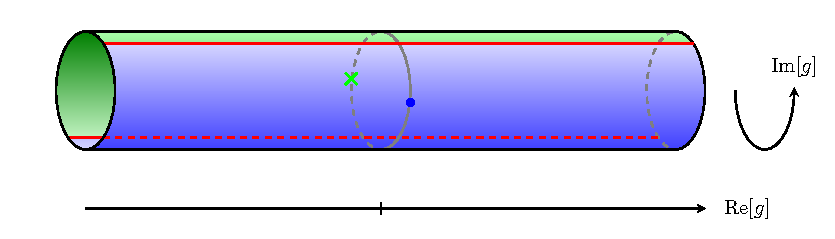
\includegraphics[width=0.68\textwidth]{\imagedir/isingCylinder.pdf}
    \caption{Phase diagram of the complexified Ising chain. The blue region indicates the basin of attraction of the trivial fixed point at $g=0$, while the green region indicates the basin of attraction of the imaginary fixed point at $g=\frac{i\pi}{2}$. The two basins are separated by a chaotic region drawn in red.}
    \label{fig:Ising}
\end{figure}

The full phase diagram of the complexified Ising chain is shown in \Cref{fig:Ising}. Since $g$ appears in an exponent accompanied by a factor of plus or minus one, we can restrain the imaginary values of $g$ to the interval $(-\frac{i\pi}{2},\frac{i\pi}{2}]$ so that $g$ is valued over an infinite complex cylinder. One way to understand the phase diagram is to think in terms of the eigenvalues $\lambda_+$ and $\lambda_-$ of the transfer matrix $T$:\footnote{We would like to thank Vladimir Rosenhaus for pointing out this interpretation}
\begin{align}
\lambda_+ = 2C \cosh(g)\,,
\hspace{20mm}
\lambda_- = -2C \sinh(g)\,.
\end{align}
The partition function, being the trace of the $N^{\rm th}$ power of the transfer matrix, can be expressed as
\begin{align}
Z=\lambda_+^N+\lambda_-^N\,.
\end{align}
The blue region in \Cref{fig:Ising} corresponds to the range $-\frac{\pi}{2}< \Im[g] <\frac{\pi}{2}$, where $|\lambda_+|>|\lambda_-|$. This means that for large systems, $\lambda_+$ dominates the free energy: 
\begin{align}
F=\log Z \approx N \log \big[C\cosh (g)\big]\,,
\end{align} 
which is the regular behavior of the Ising model. Meanwhile, the green region is the regime where $|\lambda_-|>|\lambda_+|$ so that $\lambda_-$ dominates the free energy. When $g=x+i\frac{\pi}{4}$ for some real number $x$, then $|\lambda_1|=|\lambda_2|$, and we are in the chaotic regime. In this case, for a modulus and phase given by
\begin{align}
\rho = \sqrt{\frac{\cosh(2x)}{2}}\,,\hspace{20mm} \phi = \arctan\Big[\tanh(x)\Big]\,,
\end{align}
we have that the eigenvalues and free energy equal
\begin{align}
\lambda_{\pm}=\rho e^{\pm i\phi}\,, \hspace{20mm} F = N\log(\rho)+\log\Big[2\cos(N\phi)\Big].
\end{align}
Because of the phase in the argument of the cosine, the second contribution could be arbitrarily large, depending on the exact number of sites in the Ising model. Moreover, let us consider the two-point functions and its large $N$ behavior when $\left|\lambda_+\right| > \left|\lambda_-\right|$:
\begin{gather}
\braket{\sigma_i \sigma_{i+k}} = \frac{\tr\left[T^{N-k}\sigma_3 T^k \sigma_3 \right]}{\tr\left[T^N \right]} = \frac{\lambda_+^k \lambda_-^{N-k}+\lambda_-^k \lambda_+^{N-k}}{\lambda_+^N+\lambda_-^N}  \approx \left(\frac{\lambda_{-}}{\lambda_{+}}\right)^k, \quad N\gg k\,.
\end{gather}
This correlation function behaves smoothly in the thermodynamic limit $N\to \infty$.  Meanwhile, on the special line $g= x + i \frac{\pi}{4}$,
\begin{gather}
\braket{\sigma_i \sigma_{i+k}} = \frac{\cos\, (N-2 k ) \phi}{\cos N \phi},
\end{gather}
which is highly sensitive to the total number of the sites and does not admit a simple thermodynamic limit. 

Having closely studied this simple chaotic chain, it is not hard to conceive the implications of  chaotic RG transformation in systems in higher dimensions or composed of different types of spin-sites. Roughly speaking, while an ideal gas is well-described simply be specifying temperature, pressure, and volume, for a {\it RG chaotic} gas composed of a macroscopic number of particles it would require knowledge of on the order of $10^{23}$ parameters to make accurate predictions.



\section{Baker's map, the Smale Horseshoe, and Shilnikov Homoclinic Orbits}
\label{sec:Shilnikov}
In this section, we review one of the few general tools for diagnosing chaos in a continuous dynamical system: Shilnikov homoclinic orbits. In order to properly understand these orbits, we will need to review certain facts concerning chaos in discrete dynamical systems. Consider therefore the discrete map known as the baker's map \cite{hopf1937erg}, which acts on the unit square $I = \left\{(x,y): 0 \leq x,y \leq 1 \right\}$ as
\begin{gather}
B(x, y) =\left(2x - \left\lfloor 2x \right\rfloor,\ \frac{ y + \left\lfloor 2x\right\rfloor }{2}\right),\quad B:I \to I\,.
\end{gather}
On an intuitive level, we simply stretch the unit square by a factor of two in the $x$ direction and squeeze it by a factor of two in the $y$ direction such that the total area is preserved, and afterwards we cut off the right half of the stretched shape and place it on top of the left half\footnote{The name baker's map derives from the similarity of this process with the kneading of dough.}. See \Cref{fig:baker}. 
\begin{figure}
    \centering
  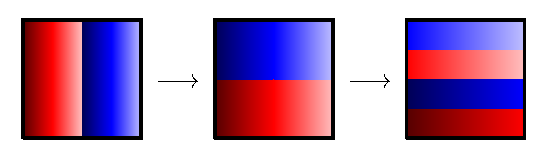
\includegraphics{\imagedir/Baker.pdf}
    \caption{Baker's Map}
    \label{fig:baker}
\end{figure}
It can be seen that the map is chaotic by associating to each point $(x,y)$ of the unit square $I$ an infinite sequence of numbers $\sigma =\left\{ \sigma_i \right\}^\infty_{i=-\infty}$, $\sigma_i \in \{0,1\}$, defined via the binary expansions of $x$ and $y$ as
\begin{gather}
x = \sum\limits^\infty_{i=1} \frac{\sigma_i}{2^{i}}\,,
\hspace{20mm}
y= \sum\limits_{i=0}^{\infty} \frac{\sigma_{-i}}{2^{i+1}}\,.
\end{gather}
The baker's map acts on $\sigma$ by shifting each number one step to the right:
\begin{gather}
\tilde{\sigma} \equiv   B(\sigma)  = \left\{ \tilde{\sigma}_i=\sigma_{i-1} \right\}^\infty_{i=-\infty}\,.
\end{gather}
From this fact one can immediately infer certain chaotic properties of the system as we did for the Bernoulli map in the previous section. For instance, given any sequence $\sigma_T$ that is periodic with a given period $T$, the orbit of $\sigma_T$ under repeated applications of the map $B$ will in turn be periodic with period $T$. And the set of all points $(x,y)$ with a periodic sequence $\sigma$ is dense in the unit square. If we take $x$ and $y$ to be irrational, the orbit of $(x,y)$ never returns to the original point. And the set of points $(x,y)$ with irrational $x$ and $y$ is also dense in the unit square. Hence, the fate of any orbit of the baker's map is infinitely sensitive to initial conditions.
\begin{figure}
    \centering
  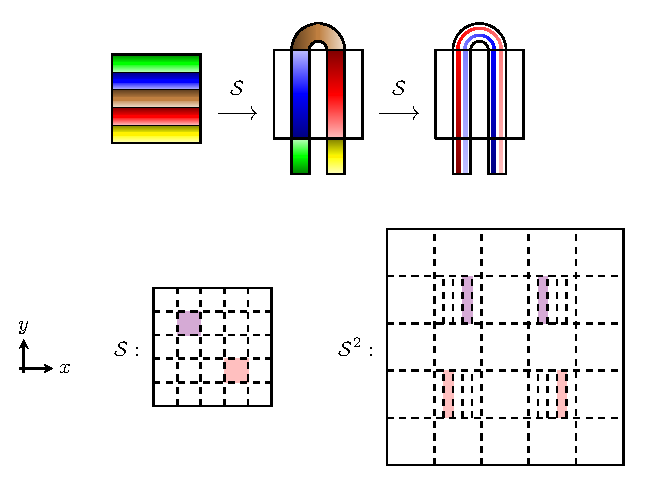
\includegraphics[width=0.7 \textwidth]{\imagedir/Smale.pdf}
    
    \caption{Above: the Smale Horseshoe map. We extend the square in the vertical direction and then bend it in the middle. Below: Regions that necessarily contain fixed points under one and two applications of the horseshoe map. The total point set that is periodic under the horseshoe map forms an infinite fractal set.}
    \label{fig:SHmap}
\end{figure}

The baker's map is a limiting case of a more general chaotic map known as the Smale horseshoe map \cite{smale1967differentiable} and depicted in \Cref{fig:SHmap}. We will denote this map by $\mathcal{S}$. One can argue that the map is chaotic by showing that it contains a fractal set of periodic orbits. To see why this is so, consider the two highlighted regions on the lower left in \Cref{fig:SHmap}. Each of these regions must necessarily contain a fixed point under the horseshoe map. Take for example the \textcolor{pink}{pink} region. In this region, red is mapped to red in the color scheme of the top part of \Cref{fig:SHmap}. Since the pre-image in this region sweeps through the entire red palette, there must necessarily be some horizontal line where image and preimage of $\mathcal{S}$ have identical hues, i.e. where the $y$-component is unchanged by $\mathcal{S}$. By instead drawing the horseshoe map with a color palette that runs from left to right, one can similarly argue that there is exists a vertical line in the \textcolor{pink}{pink} region, where the $x$-component is unchanged by $\mathcal{S}$. At the intersection of the vertical and horizontal lines just described, there must be a fixed point. By the same argument, it is not hard to see that $\mathcal{S}^2$ must have a fixed point in each of the four regions highlighted in the lower right of \Cref{fig:SHmap}, and that in general $\mathcal{S}^n$ must have $2^n$ fixed points. From this line of reasoning, it becomes apparent that $\mathcal{S}$ contains a Cantor set of periodic orbits with all possible periods, which furnishes evidence to the fact that the Smale horseshoe map is chaotic. Furthermore, it can be rigorously proved that any map topologically equivalent to the Smale horseshoe map is also chaotic \cite{guckenheimer2013nonlinear}. 


So far we have reviewed discrete dynamical systems, but we now turn to continuous dynamical systems described by a set of autonomous first-order differential equations. For such systems, it is also possible to establish the presence of chaos via the horseshoe map. To do this, one needs a way of deriving a two-dimensional discrete map from a system of differential equations. This is achieved with the Poincar\'e map: given a continuous dynamical system in more than two dimensions, we consider some fixed two-dimensional surface $S$ that is traversed by the trajectories of the dynamical system. For any point $s_0 \in S$ there is a unique solution curve that passes through $s_0$. Suppose this curve is such that we can follow it forward in time starting at $s_0$ until we find that it crosses $S$ again at some point $s_1$. For all such points $s_0$, the Poincar\'e map $\pi$ is defined by the relation $\pi(s_0) = s_1$.

From the above discussion, we see that whenever in a continuous dynamical system we are able to find a Poincar\'e map that induces a Smale horseshoe map, then we know that the system is chaotic. A simple set of sufficient criteria for making this determination was found by Shilnikov \cite{shilnikov1965case}, who managed to prove that a three-dimensional system is chaotic if it contains a homoclinic orbit originating and terminating at a fixed point such that the stability matrix at this point has a pair of complex conjugate eigenvalues $\lambda_\pm = -\rho \pm i \omega$ and a real eigenvalue $\lambda_3=\gamma > \rho$. The proof runs roughly as follows: In the vicinity of the fixed point, the dynamical system can be described by coordinates $x$, $y$, and $z$ satisfying the equations
\begin{gather}
    \begin{array}{rclcl}
\dot x &=&  -\rho x - \omega y &+& F_1(x,y,z) \,,\\
\dot y &=& ~~\omega x - \rho y  &+& F_2(x,y,z)\,,\\
\dot z &=& \gamma z &+& F_3(x,y,z)\,,
\end{array}
\end{gather}
where $F_i(x,y,z)$, $i \in \{1,2,3 \}$, are functions of second order or higher in the coordinates.
Suppose now we surround the fixed point by a cylindrical shell whose curved surface is given by $C=\left\{(x,y,z): x^2+y^2 = r^2 , |z| \leq h \right\}$, see \Cref{fig:Shilnikov}. The homoclinic orbit enters the cylinder through the curved surface at some point $p$ (marked in \textcolor{brown}{brown} in \Cref{fig:Shilnikov}) and exits at some point $q$ (marked in \textcolor{teal}{teal} in \Cref{fig:Shilnikov}) on the flat top of the cylinder. By taking $r$ and $h$ to be very small, we can assume that $q$ is situated on the $z$-axis and that $p$ lies in the $(x,y)$-plane so that we can choose to write $q=(0,0,h)$ and $p=(r,0,0)$. Disregarding the higher-order terms $F_i(x,y,z)$, we determine that the solution curves near $p$ are given in terms of local coordinates $(\zeta,\theta)$ by
\begin{align}
    x(t) =&\, r e^{-\rho t} \cos(\omega t + \theta)\,, \notag  \\
    y(t) =&\, r e^{-\rho t} \sin(\omega t +\theta)\,,\\
    z(t) =&\, \zeta e^{\gamma t}\,. \notag 
\end{align}
In this approximation, any given solution curve, intersecting $C$ at time $t=0$ at a positive value $\zeta$ of $z$, subsequently intersects the plane $z=h$ at the coordinates
\begin{gather}
\left\{
\begin{matrix}
    x(\theta,\zeta) = r\left(\frac{\zeta}{h}\right)^{\frac{\rho}{\gamma}} \cos\left(\theta - \frac{1}{\lambda} \log \frac{\zeta}{h}\right),\\
    y(\theta,\zeta) = r\left(\frac{\zeta}{h}\right)^{\frac{\rho}{\gamma}} \sin\left(\theta - \frac{1}{\lambda} \log \frac{\zeta}{h}\right).
\end{matrix}\right.    
\label{eq:fPM}
\end{gather}
\begin{figure}
    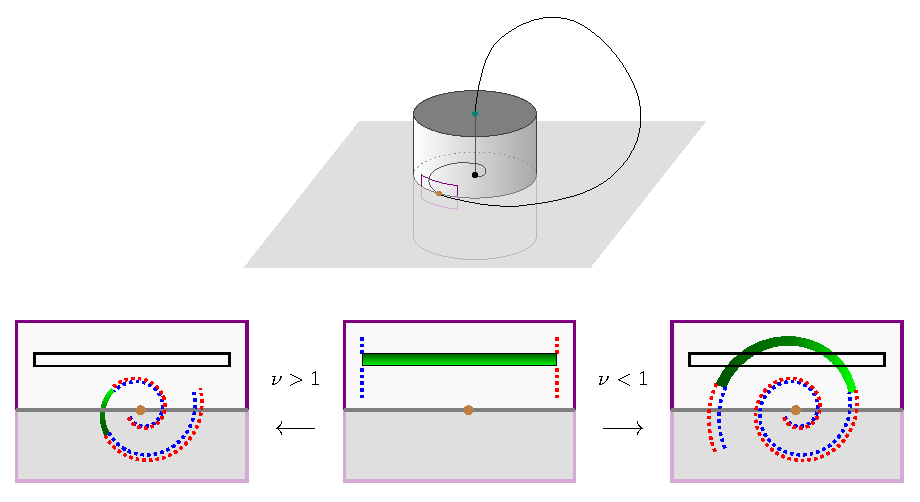
\includegraphics[width=1.0\textwidth]{\imagedir/Shilnikov.pdf}
    \caption{Homoclinic orbit and the Poincar\'e map \cref{eq:ShilProof} that it induces for different values of the ratio $\nu = \frac{\rho}{\gamma}$. For $\nu<1$ it is always possible to find a subregion that undergoes a Smale horseshoe map as shown on the right. For $\nu>1$ this is not the case.}
    \label{fig:Shilnikov}
\end{figure}
For tiny values of $x$ and $y$, the solution curve will be close to the homoclinic orbit and will flow back to again intersect the surface $C$ at some point close to the point $p$. Thereby, the flow induces a Poincar\'e map that maps points on $C$ with $z > 0$ back to $C$. To first order in $x$ and $y$ we can approximate this map by a linear transformation:
\begin{gather}
    \left\{
    \begin{matrix}
    \zeta' =A x(\theta,\zeta) + B y(\theta,\zeta),\\
    \theta' = C x(\theta,\zeta) + D y(\theta,\zeta).
    \end{matrix} \right. \label{eq:sPm}
\end{gather}
Combining the equations \cref{eq:fPM} and \cref{eq:sPm} we arrive at the following map:
\begin{gather}
        \left\{
    \begin{matrix}
    \zeta' = r\left(\frac{\zeta}{h}\right)^{\frac{\rho}{\gamma}} \left[ A  \cos\left(\theta - \frac{1}{\lambda} \log \frac{\zeta}{h}\right) + B  \sin\left(\theta - \frac{1}{\lambda} \log \frac{\zeta}{h}\right)\right],\\
    \theta' = r\left(\frac{\zeta}{h}\right)^{\frac{\rho}{\gamma}}\left[ C  \cos\left(\theta - \frac{1}{\lambda} \log \frac{\zeta}{h}\right) + D  \sin\left(\theta - \frac{1}{\lambda} \log \frac{\zeta}{h}\right)\right].
    \end{matrix} \right. \label{eq:ShilProof}
\end{gather}
For generic values of $A$, $B$, $C$, and $D$, vertical lines of constant $\theta$ and increasing $\zeta$ are mapped to spirals that wind outward around the origin as sketched in \Cref{fig:Shilnikov}. Now, the key observation is that for $\nu \equiv \frac{\rho}{\gamma} < 1$, when $\frac{\zeta}{h}$ is small as required for the approximation \cref{eq:ShilProof} to be valid, points $(\zeta,\theta)$ are mapped to points $(\zeta',\theta')$ that are farther from the origin. For this reason, drawing a plot of the map \cref{eq:ShilProof} as in \Cref{fig:Shilnikov}, one finds that when the Shilnikov condition
\begin{align}
\nu < 1 \label{eq:ShilnikovCondition}
\end{align}
is satisfied, then generically it is always possible to find a region of $C$ that undergoes a Smale horseshoe map. This concludes our proof sketch of Shilnikov's theorem. In the next section, we present examples of Shilnikov homoclinic orbits that occur in the context of RG flow.


\section{Chaotic Bi-Antisymmetric Tensor Model}\label{sec:model}
\label{sec:QFT}
In this section, we present a family of tensor models \cite{Klebanov:2016xxf,Klebanov:2018fzb} with $O(N_1)\times O(N_2)$ symmetry and show that for special non-integer values of $N_1$ and $N_2$, the RG flows of the models become chaotic.\footnote{ For an interesting large $N$ limit of a model with $SO(N_1)\times SO(N_2)$ we refer the reader to \cite{Chaudhuri:2020xxb,kapoor2021bifundamental}} In studying the RG flow of a model whose symmetry group is of non-integer size, we follow the program of \cite{Jepsen:2020czw} and \cite{Jepsen2021HomoclinicRG}, which in this setting discovered the existence of RG limit cycles and homoclinic orbits. Generally, models with non-integer dimensional symmetry groups can be studied numerically and analytically \cite{Binder:2019zqc,gorbenko2018walking}, can describe real physical phenomena \cite{de1979scaling}, and avoid the famous $a,c,F-$ theorems \cite{zamolodchikov1986irreversibility,Komargodski:2011vj,Klebanov:2011gs,Jafferis:2011zi} at the price of non-unitarity. For to study non-monotonic RG-flow it is necessary to consider regimes where the Zamolodchikov metric has negative eigenvalues, which implies that some of the two-point functions are equipped with negative coefficients.

The main advantage to treating $N_1$ and $N_2$ as real numbers that we can tune to any desired value lies in the fact that this approach allows us to apply theorems of bifurcation theory, which provide one of the sole means of firmly establishing that a dynamical system is chaotic. The idea to treat $N$ in the $O(N)$ model as a bifurcation parameter was suggested already in Ref. \cite{Damgaard:1991zb}. Ref. \cite{ibanez1995sil} proved that in a general class of 4-parameter dynamical systems, it is possible to tune the parameters to such values that generically Shilnikov chaos is guaranteed to occur. Ref. \cite{ibanez2005shil} improved these results by proving that Shilnikov homoclinic orbits arise in some systems in the vicinity of a certain kind of codimension-3 bifurcation. Finally, Ref. \cite{baldoma2020hopf} provided rigorous evidence for the generic presence of Shilnikov chaos in a codimension one subset of two-parameter families of dynamical systems that undergo a subtype of the codimension-2 bifurcation known as the zero-Hopf (ZH) bifurcation. In the tensor models we present in this section, this kind of bifurcation is realized.

We consider a family of scalar models described by rank-four tensor fields $\phi^{ab}_{\alpha\beta}$ where the upper indices run from one to $N_1$: $a_1,a_2 \in\{1,...,N_1\}$ and belong to the antisymmetric representation of the $O(N_1)$ group, while the lower indices run from one to $N_2$: $\alpha,\beta\in\{1,...,N_2\}$ and also belong to the antisymmetric representation of the $O(N_2)$ group:
\begin{align}
\phi^{ab}_{\alpha\beta} = -\phi^{ba}_{\alpha\beta} = \phi^{ba}_{\beta\alpha}\,.
\end{align}
We work in $d=4-\epsilon$ Euclidean dimensions, where quartic interactions in the fields are marginally relevant. Unlike the case for $N_1$ and $N_2$, the number of spacetime dimensions $d$ being non-integer valued is not crucial to the realization of RG chaos in this section. The effect of working in slightly less than four dimensions is to introduce small linear terms into the beta functions for the coupling constants we introduce below. The same effect can be achieved by coupling the model to gauge fields, but for simplicity of presentation, we do not adopt this approach but work in $4-\epsilon$ dimensions instead.

In total the family of models has eight marginal, quartic interactions $O_i$, and we take the action to be
\begin{align}
S = \int d^dx\bigg[\frac{1}{2}(\partial_\mu \phi^{ab}_{\alpha\beta})^2
+\frac{1}{4!}\sum_{i=1}^8g_i\,O_i(x)\bigg]\,, \label{eq:action}
\end{align}
where the operators $O_i$ are given by
\begin{align}
&O_1= \Big(\phi^{ab}_{\alpha\beta}\,\phi^{ab}_{\alpha\beta}\Big)^2\,,
\hspace{28mm}
O_2= \phi^{ab}_{\alpha\beta}\,\phi^{ab}_{\gamma\delta}\,\phi^{cd}_{\gamma\delta}\,\phi^{cd}_{\alpha\beta}\,,
\notag
\\
\label{eq:operators}
&O_3= \phi^{ab}_{\alpha\beta}\,\phi^{ab}_{\gamma\beta}\,\phi^{cd}_{\gamma\delta}\,\phi^{cd}_{\alpha\delta}\,,
\hspace{22mm}
O_4= \phi^{ab}_{\alpha\beta}\,\phi^{cb}_{\alpha\beta}\,\phi^{cd}_{\gamma\delta}\,\phi^{ad}_{\gamma\delta}\,,
\\
&O_5= \phi^{ab}_{\alpha\beta}\,\phi^{ab}_{\gamma\delta}\,\phi^{cd}_{\alpha\delta}\,\phi^{cd}_{\gamma\beta}\,,
\hspace{22mm}
O_6= \phi^{ab}_{\alpha\beta}\,\phi^{cd}_{\alpha\beta}\,\phi^{ad}_{\gamma\delta}\,\phi^{cb}_{\gamma\delta}\,,
\notag
\\
&O_7= \phi^{ab}_{\alpha\beta}\,\phi^{cb}_{\gamma\beta}\,\phi^{cd}_{\gamma\delta}\,\phi^{ad}_{\alpha\delta}\,,
\hspace{22mm}
O_8= \phi^{ab}_{\alpha\beta}\,\phi^{cb}_{\gamma\delta}\,\phi^{cd}_{\gamma\beta}\,\phi^{ad}_{\alpha\delta}\,.
\notag
\label{eq:oper}
\end{align}
\begin{figure}
\centering
  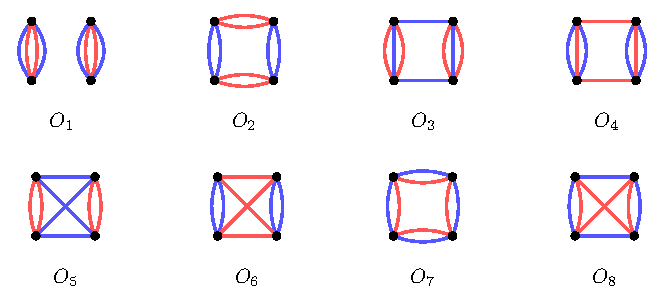
\includegraphics{\imagedir/operators.pdf}
\caption{Graphical representation of the operators \cref{eq:oper}}
\label{fig:oper}
\end{figure}
Diagrammatically, these operators can be represented as in \Cref{fig:oper}. The beta functions for the coupling constants associated to these operators admit of a perturbative expansion:
\begin{align}
\beta_{g_i}= \mu\frac{dg_i}{d\mu}=-\epsilon g_i+\beta_{g_i}^{(2)}+\mathcal{O}(\| \vec g \|^3)\,,
\end{align}
where $\mu$ is the renormalization group scale. The first term on the RHS represents the naive scalings of the interactions and the terms $\beta_{g_i}^{(2)}$ indicate the lowest-order loop corrections, which are quadratic in the coupling constants. Owing to the large number of operators that mix under the RG flow, analyzing the dynamics of this family of tensor models, even numerically, poses a challenge. Future exploration of exotic QFTs may uncover chaos in smaller systems. But since perturbative beta functions are polynomials with a finite number of roots, by the Poincar\'e-Bendixson theorem chaos cannot occur in continuous theories unless there are at least three coupling constants.

We will adopt the perspective of thinking of the beta functions abstractly as an 8-dimensional 2-parameter dynamical system:
\begin{align}
\label{eq:fullsystem}
\frac{dg_i}{dt}=\beta_{g_i}(g_j,N_1,N_2)\,.
\end{align}
Here $t=\log\mu$. Using general formulas for perturbative beta-functions in $4-\epsilon$ dimensions, a straightforward computation yields $\beta_{g_i}^{(2)}$ as functions of the ranks $N_1$ and $N_2$ of the symmetry groups. We list the results in \cref{appendix:beta}, where explicit formulas for $\beta_{g_i}^{(2)}$ are given. Since the upper and lower indices of the fundamental fields $\phi^{ab}_{\alpha\beta}$ transform in the same kind of representation, in the family of QFTs we are considering, the theory with $O(N_1)\times O(N_2)$ symmetry is the same as the theory with $O(N_2)\times O(N_1)$. This fact is reflected in the beta functions, which are invariant under the simultaneous interchange of $N_1\leftrightarrow N_2$, $g_3\leftrightarrow g_4$, and $g_5 \leftrightarrow g_6$.

When we take $N_1$ and $N_2$ to be integers greater than three, the system of beta-functions describes the behavior of a real unitary quantum field theory, and therefore we expect only regular solutions to the system. The solutions curves are all heteroclinic orbits --- trajectories that connect separate fixed points --- and one can find a Zamolodchikov metric for the system and check that indeed the $a-$theorem is satisfied. In \cref{appendix:metric} we show the precise form of the metric to leading order in perturbation theory, where the metric is independent of the coupling constants but depends only on $N_1$ and $N_2$. Meanwhile, if $N_1$ or $N_2$ is equal to two or three, the eight operators \cref{eq:operators} will no longer be independent as there will exist vanishing linear combinations. And if $N_1$ or $N_2$ is equal to one, all eight operators vanish.

In the following, we continue the system to fractional values of $N_1$ and $N_2$. The regime where  either $N_1$ or $N_2$ lies between $-2$ and $3$ is particularly interesting for our purposes, for here the Zamolodchikov metric becomes sign-indefinite, so that the RG flow is no longer constrained to be monotonic. It therefore becomes possible for the RG flow to exhibit limit cycles, homoclinic orbits, and chaos. Our focus will be on investigating the presence of chaos. To this end, we look for ZH bifurcations \cite{takens1974singularities,guckenheimer2013nonlinear,Kuznetsov2004} in the space of $N_1$ and $N_2$. In other words, we are interested in the existence of special fixed points such that
\begin{gather}
\begin{cases}
    \displaystyle    \beta_i\left(g_j,N_1,N_2\right) = 0\,,
    \vspace{2mm}
    \\
    \displaystyle
    \det\left(\frac{\partial \beta_i}{\partial g_j}\right) = 0\,, 
    \vspace{2mm}
    \\
    \displaystyle
    \det\left(\frac{\partial \beta_i}{\partial g_j}-\lambda\right) - \text{has a pair of imaginary roots in $\lambda$}. 
    \end{cases}
    \label{eq:ZHcond}
\end{gather}
The last requirement can be formulated in terms of a closed algebraic equation, but for brevity we will skip it and refer the reader to \cite{Jepsen2021HomoclinicRG}. In total, the conditions \cref{eq:ZHcond} consist of $8+2$ equations, so that generically one expects a discrete set of solutions in the space of eight couplings $g_i$ and two parameters $N_1$ and $N_2$. 
In the vicinity of a ZH point it is possible to make a coupling constant redefinition $\left\{g_i\right\} \to \left\{x,y,z,\mathfrak{g}_i\right\}$, a parameter redefinition $(N_1,N_2) \to (a,b,\eta)$, and a reparametrization $t\rightarrow \tau(t)$ in such a way that the system of differential equations furnished by the beta functions can be brought into the so-called truncated normal form 
parameterized by coordinates $x,y,z$:
\begin{gather}
\begin{cases}
\displaystyle    \frac{dx}{d\tau} = y +\eta x- axz\,, 
\vspace{2mm}
\\
\displaystyle       \frac{dy}{d\tau} = -x+\eta y-ayz\,,
     \label{eq:ZHnormform}
     \vspace{2mm}
    \\
\displaystyle   
    \frac{dz}{d\tau} = -\beta+z^2+b(x^2+y^2)\,.
\end{cases}
\end{gather}
These equations are approximate in that we are omitting terms of cubic and higher order in the coordinates. The parameters $a,b,\eta,\beta$ depend on $N_1$ and $N_2$, with $a$, $\mu$, and $\eta$ being real-valued, while $b=\pm 1$. Right at the ZH point $\beta$ and $\eta$ equal zero. The other coupling constants $\mathfrak{g}_i$ decouple from the rest at this order of expansion. The two-parameter invariant manifold given by $\mathfrak{g}_i=0$ is known as the center manifold. There is a definite procedure for computing the higher order terms on the center manifold, order by order, although the higher order terms never terminate. In \cref{appendix:normalForm} we present the explicit transformation that puts the beta functions into the truncated normal form. 



The system of equations \cref{eq:ZHnormform} has 6 topologically distinct types of behaviors, depending on whether $b$ equals plus or minus one and on whether $a>-1$, $a\in (-1,0)$, or $a>0$. We are interested in the type with $a,b>0$. The recent result of \cite{baldoma2020hopf} is that in two-parameter dynamical systems with ZH points of this type, there will generically exist nearby parameter values for which the systems exhibit Shilnikov homoclinic orbits and hence chaos. For the system of beta-functions governing the RG flows of the tensor models \cref{eq:action}, as given in \crefrange{eq:beta1}{eq:beta8} in \cref{appendix:metric}, it can be verified that there is a ZH point of the particular type in question situated at \sisetup{round-mode=figures,round-precision=4}
\begin{align}\label{eq:ZH}\tag{ZH}
&        \begin{pmatrix*}[r]
        N_1^* \\
        N_2^*
    \end{pmatrix*}= \begin{pmatrix*}[r]
        \num{2.520427996662252} \\
        \num{1.972260741688210} 
    \end{pmatrix*},
    \vspace{3mm}
    \\
    g^\ast \equiv
\big(
    \num{31.01364336772574},\,
    \num{14.90146693485237},\,&
    \num{8.879972225165773},\,
    \num{136.1544856591584},\,
    \num{3.810504206934431},\,
    \num{-143.4849700979769},\,
    \num{-18.64425623143404},\,
    \num{18.15961700372116}
    \big) \epsilon\,.
    \nonumber
\end{align}
For this ZH point the quadratic normal form coefficients $a,b,\eta,\beta$ in \cref{eq:ZHnormform} are given to leading order in $\delta N_1 \equiv N_1-N_1^\ast$ and $\delta N_2 \equiv N_2-N_2^\ast$ by 
\begin{align}
 a = 0.8826\,, & \hspace{10mm} b = 1\,,
 \\
 \eta =
 -40.59\,\delta N_1
 -208.3\, \delta N_2\,, &
 \hspace{10mm} \beta = -89.05\,\delta N_1-456.9\, \delta N_2\,.
 \nonumber
\end{align}
If we restrict ourselves to the second order normal form in \cref{eq:ZHnormform} and disregard the higher-order corrections for a moment, we do not find any homoclinic solutions. Depending on the values of $\delta N_1$ and $\delta N_2$, the value of $\beta$ will be either negative or positive. In the latter case, there is a pair of fixed point located at $x=y = 0$ and $z=\pm \sqrt{\beta}$. This pair of fixed point is connected by heteroclinic solutions. And therefore, at quadratic order in the dynamical variables, we do not get any new phenomena --- the system simply flows from one fixed point to another in a regular way. One of these heteroclinic solutions runs vertically between the two fixed points, the $z$ axis being an invariant manifold of the flow \cref{eq:ZHnormform}. In the special case when we tune $\delta N_1$ and $\delta N_2$ so as to set $\eta=0$, the remaining heteroclinic solutions admit of a simple description, being orbits that wind around the invariant ellipsoid given by
\begin{align}
z^2+\frac{b}{1+a}(x^2+y^2)=\beta\,.
\end{align}
Once we cease to neglect higher order terms in the normal form, these terms mix the {\it heteroclinic} solutions, and {\it homoclinic} solutions emerge. Essentially, once we perturb the system, an initially vertical orbit flowing from one fixed point will now stray slightly from the $z$-axis and miss the other fixed point and can instead merge onto the erstwhile invariant ellipsoid and flow back to the fixed point whence it originated. Whenever these homoclinic solutions satisfy the Shilnikov condition \cref{eq:ShilnikovCondition}, chaos ensues.

\begin{figure}
    \centering
    \includetikz{homoclinic_orbit_reduced_system}
    \caption{Homoclinic orbit to the saddle-focus at $(u,v,x) \approx (0.0008, -0.0001, 0.0152)$ in the RG flow of coupling constants at parameter values $(N_1-N_1^*,N_2-N_2^*)=( \num{7.41174e-8},\num{-5.05368e-7})$. Here $u$, $v$, and $x$ are three independent functions of the couplings $g_i$, with their precise forms given in \cref{appendix:normalForm}. For computationally reasons, we additionally scaled the variables $u,v$ and $x$ by a factor $10000/(6(32\pi)^2\epsilon)$. In the language of \cref{sec:Shilnikov}, the fixed point of the homoclinic orbit has eigenvalues $\lambda_{\pm}\approx -0.0020 \pm 0.0307i$  and $\lambda_3 \approx 0.0047$. Thus, the Shilnikov condition is satisfied, and the dynamics near the saddle-focus are complex.
    \label{fig:homoclinic1}}
\end{figure}

For a given ZH point in parameter space, it is a non-trivial task to determine the nearby parameter values for which the dynamical systems exhibit Shilnikov homoclinic orbits. There are no homoclinic asymptotics available as is the case for example in the generic Bogdanov-Takens bifurcation, see \cite{Bosschaert@Interplay}. Our approach has been to first search for homoclinic solutions in the parameter space of $N_1$ and $N_2$ in the 3-dimensional reduced and truncated system \cref{eq:reducedsystem} on the center manifold  with cubic terms added in. Subsequently, we were able to uplift these approximate solutions to convergent homoclinic solutions in the full 8-dimensional systems.  This was achieved as follows: a homoclinic orbit starts and ends at a fixed point.  The fixed points are not hard to find numerically, since this amounts to setting the beta functions equal to zero and solving the resulting algebraic equations. Once we have a fixed point, we numerically integrate the system, searching for solutions where the one-dimensional unstable manifold of the fixed point is reinjected into its two-dimensional stable manifold. In \Cref{fig:homoclinic1} such a solution in the reduced system is shown, while in the left panel of \Cref{fig:homoclinic1_profiles} the profiles are given. This solution is then translated to the full system and subsequently corrected by applying Newton's method to a special boundary value problem, see \cite{DeWitte2012}. The right panel of \Cref{fig:homoclinic1_profiles} displays an example of a Shilnikov homoclinic orbit that we located in the vicinity of the ZH bifurcation point \cref{eq:ZH} in the full system.  This solution in then continued using standard pseudo-arclength continuation, see for example \cite{Beyn2002149}.  In the 2-dimensional parameter space spanned by $N_1$ and $N_2$, we observe Shilnikov homoclinic orbits to occur along a one-dimensional subspace that constitutes a wiggling curve emanating from the ZH point, as shown in \Cref{fig:wigcurve}. Note that there are two wiggling curves. Indeed, by reversing time, we can use the same method as outlined above to find the second curve of homoclinic orbits. This behavior in parameter space conforms to the general pattern for ZH points of this subtype, as explained in Ref. \cite{champneys2004entwined}, of homoclinic orbits occurring along an oscillating curve in a wedge-shaped region whose thickness decays exponentially as you approach the ZH point. 

\begin{figure}
    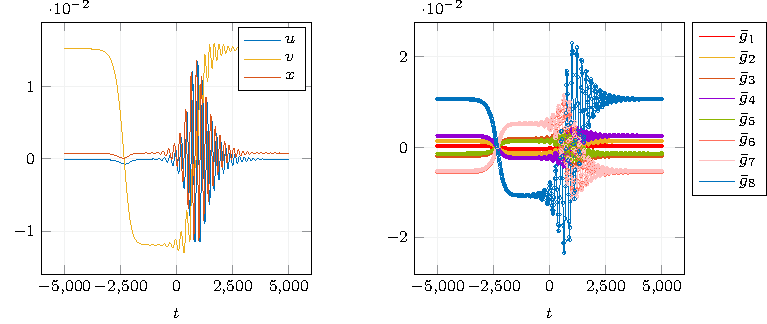
\includegraphics{\imagedir/homoclinic_profiles_groupplot.pdf}
    \caption{In the left panel the profiles of the homoclinic orbit in the reduced system at parameter values $(N_1-N_1^*,N_2-N_2^*)=( \num{7.41174e-8},\num{-5.05368e-7})$, see \Cref{fig:homoclinic1} are shown. In the right panel, a homoclinic solution in the full 8-dimensional space of coupling space at the parameter values $(N_1-N_1^*, N_2-N_2^*)\approx(\num{1.053235334346889e-7}, \num{-6.655194199241109e-7})$. The abscissa represents the span of $t=\log \mu$ truncated to the interval $[-5000, 5000]$, the ordinate indicates values of the eight-coordinates $\bar g$ of the system obtained translating the ZH point to the origin in \cref{eq:fullsystem} and scaling the resulting coordinates by a factor $10000/(6(32\pi)^2\epsilon)$.
    The solid lines represent the approximated solution, while the circles are the Newton corrected solution. We see that at this scale they are indistinguishable.
     }
    \label{fig:homoclinic1_profiles}
\end{figure}


We have now ascertained that for a special curve of values for $N_1$ and $N_2$, Shilnikov homoclinic orbits are present in the two-parameter class of dynamical systems \cref{eq:fullsystem}. This means that for the family \cref{eq:action} of tensor models, there exists a special codimension one subset of theories whose RG flows contain Shilnikov homoclinic orbits. By the argument reviewed in \cref{sec:Shilnikov} it follows that for each of these theories, with fixed $N_1$ and $N_2$, the space of coupling constants contains, in addition to a homoclinic orbit, a fractal set of periodic orbits with an infinite range of periodicities. Hence, we conclude that each of these theories exhibits a chaotic RG flow: an arbitrarily tiny change of initial values for the coupling constants can spell the difference between the couplings flowing to a fixed point or them winding endlessly around a loop.

One can object that we are merely working at leading order in perturbation theory in $\epsilon = 4-d$, and that higher loop corrections will modify the RG flow. But the presence of a ZH bifurcation is stable under small deformations, and \cite{baldoma2020hopf} proved rigorously that the presence of Shilnikov homoclinics in a subspace of systems near a ZH point is a generic phenomenon. Since higher-order corrections are suppressed in $\epsilon$, as long as we take $\epsilon$ to assume a tiny value we can reliably state that the RG flow is in fact chaotic. 

As a symptom of the chaos, it is possible to find a number of interesting or bizarre RG trajectories that arise as we slightly change the initial conditions. We saw above that a homoclinic orbit arises as a heteroclinic orbit is disturbed, such that an orbit originating from one fixed point misses the other fixed point, but winds back to its starting point. By further perturbing this orbit, it is possible to make it miss the starting point and instead flow once more towards the other fixed point, miss it again and wind back whence it originated. Such an orbit is called a 2-pulse homoclinic orbit. Through additional careful deformations, one can find 3-, 4-, 5-, ... pulse homoclinic obits, which densely occupy the neighborhood of the Shilnikov homoclinic orbit. As an example, we display a 3-pulse homoclinic orbit in \Cref{fig:3pulse}. 






\section{Discussion and Outlook}

\begin{figure}
    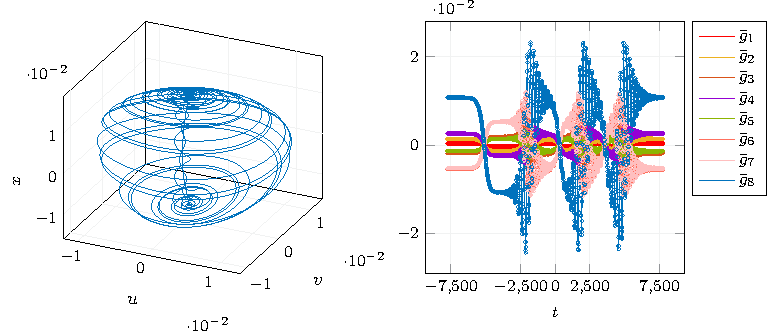
\includegraphics{\imagedir/3pulse_groupplot.pdf}
    \caption{The left panel: Three-pulse homoclinic orbit to the saddle-focus at $(u,v,x) \approx (0.0153, 0.0008, -5.0736 \times 10^{-5})$ in the RG flow of coupling constants at parameter values $(N_1-N_1^*,N_2-N_2^*)=( \num{5.144712958706644e-8},\num{-3.915956879261614e-7})$. Here $u$, $v$, and $x$ are three independent functions of the couplings $g_i$, with their precise forms given in \cref{appendix:normalForm}.
    The right panel: the profile of the three-pulse homoclinic solution in the shifted and scaled 8-dimensional phase-space.
    \label{fig:3pulse}}
\end{figure}


\begin{figure}
    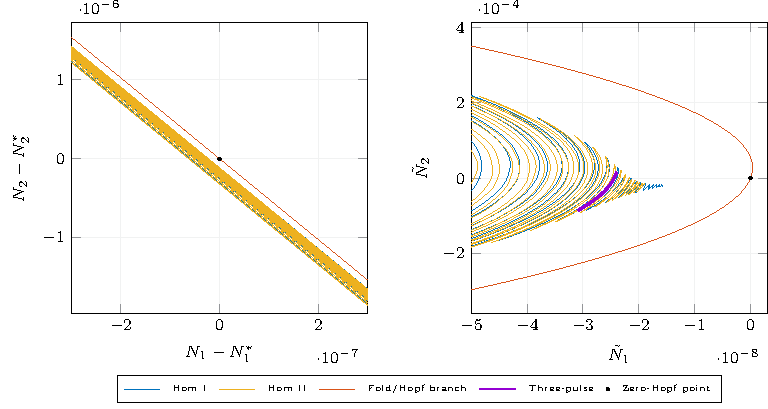
\includegraphics{\imagedir/wiggling_groupplot.pdf}
    \caption{The left panel: Entwined wiggling of loci of homoclinic orbits emanating from the zero-Hopf bifurcation point in the shifted parameter space $(N_1-N_1^*,N_2-N_2^*)$. The right panel: Same curves as in the left panel, but rotated clockwise through the angle $0.1925$. Also, a bifurcation curve (purple) of three-pulse Shilnikov homoclinic orbits is shown in the right panel.
    }
    \label{fig:wigcurve}
\end{figure}

In this paper, we have presented examples of QFTs with chaotic RG flows. Usually, in the study of the renormalization group, one considers flows that are non-chaotic and thereby give rise to universality --- the behavior of a system at the macroscopic level is insensitive to the precise microscopic configuration of the system. Imagine that we have two adjacent balls made of the same metal. If we measure their macroscopic properties, such as the specific heat, speed of sound, and density, we would find them to be identical. But if we use an electronic microscope and discern the internal structure of these objects we would find them to be completely different: the distance between the atoms would vary, the number of atoms would be different, the exact distribution of isotopes and defects would differ, and so on. Generally, when an RG flow is non-chaotic, some parameters are irrelevant at large distances so that small alterations at short length scales do not affect the large scale description of the system. But one of the key features of any chaotic mapping is an extreme sensitivity to initial conditions. If we imagine a world with a chaotic renormalization group, macroscopic systems would be sensitive to the properties of each individual atom. In this sense, chaotic RG flows generally, and our example specifically, present a new and peculiar instance of a UV/IR mixing, where the IR behavior is extremely sensitive to the UV properties. For this reason, the study of chaotic RG flows and the demarcation of the instances where they occur pose an interesting problem. In the examples we considered, it was necessary to relax the condition of unitary, but such theories can nonetheless be studied on a lattice or find realization in cold atom experiments. And so to the question raised in the title of the paper \cite{morozov2003can}, we respond that {\it yes, RG flows can indeed end up in a total mess.} 

\begin{figure}
    % \includetikz{simulate_2_torus}
    % \hfill
    % \includetikz{torus}
    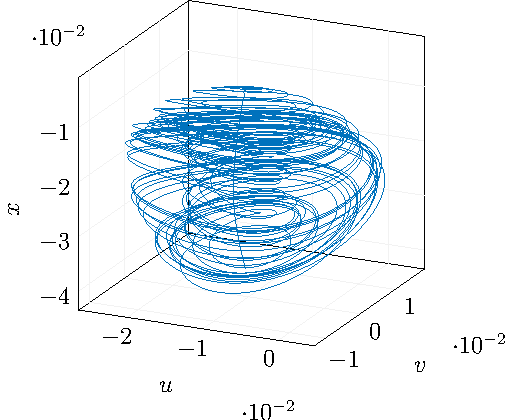
\includegraphics[width=0.5\textwidth]{\imagedir/simulate_2_torus.pdf}%
    \hfill
    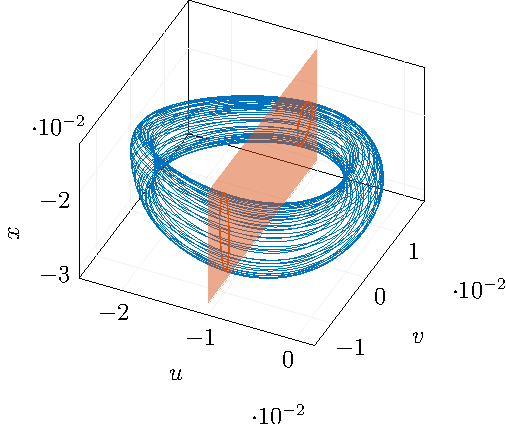
\includegraphics[width=0.5\textwidth]{\imagedir/torus.pdf}
\caption{In the left panel: A spiral attractor-like solution of the reduced system \cref{eq:reducedsystem} obtained by integrating backwards in time starting in the one-dimensional unstable manifold of the equilibrium located at $(u,v,x)\approx (\num{-0.02473081349681433},\num{-0.02190477549603949},\num{0.0014168404408595782})$ with parameter values $(N_1-N_1^*, N_2-N_2^*) = (\num{-3.4894952252725343e-6}, \num{1.7741178541515484e-5})$.
The solution convergence to a two-dimensional torus, shown in the right panel.
\label{fig:2intersol}}
\end{figure}


Having established the existence of QFTs with chaotic RG flows, it is reasonable to expect these theories to manifest period-doubling cascades, Feigenbaum scaling, strange attractors and other interesting phenomena. For the tensor model \cref{eq:action} studied in this paper, it is a formidable numerical challenge to reliably investigate exotic RG trajectories because the flow equations are 8-dimensional. But as an approximate probe of the behavior of the full system, we can study the truncated flow equations describing the reduced system on the center manifold in the hope that these solution curves can be uplifted to the full system, like we were able to do for the Shilnikov homoclinic orbits. Generally, when searching for exotic trajectories in the reduced system, we observe three kinds of solution curves:
\begin{enumerate}
\item The solution grows without bound.
\item The solution converges to a periodic cycle.
\item The solution converges to a torus.
\end{enumerate}
An example of the third scenario is depicted in \Cref{fig:2intersol}.

It is a well-known and much appreciated fact that Lagrangians, in furnishing virtually all the essential information of the QFTs they represent, provide a beautifully compact way of encoding a tremendous amount of information. We leave it as a question for future work whether this information includes the geometry of fractal patterns.



\section{Acknowledgment}

We are grateful to Igor R. Klebanov for insightful discussions and suggestions throughout the project. We are also grateful to A. Gorsky, A.Morozov, Yu.\ A. Kuznetsov, A. Milekhin, Y. Oz,  A. Polyakov, Y. Wang, S. Dubovsky and V. Rosenhaus for valuable discussions and comments. 
FKP was supported by the Russian Science Foundation (Grant No. 20-71-10073).

\begin{subappendices}
\section{General Discussion of Chaos}

\label{appendix:chaos}

 \epigraph{ “The least initial deviation from the truth is multiplied later a thousandfold”}{{\it Aristotle} \cite{Aristotle}}

It is rather hard to formulate a precise mathematical definition of chaos, and for this reason one sometimes encounters definitions of chaos of a speculative or even philosophical nature. From a pedestrian point of view, if by "chaos" we have in mind something unpredictable, the equations \cref{eq:dynsys} should not contain any chaos: if we know the initial state of a system, we can evolve it forward in time and predict all future states exactly. Due to the uniqueness and existence theorems for systems of differential equations, we know that systems subject to the same initial conditions will follow the same evolution. Therefore, we would not expect randomness or "chaos" in our dynamical system \cref{eq:dynsys}. The imaginary intellect whose full knowledge of the present universe allows it to know with certitude all future course of history is sometimes referred to as Laplace's demon.  But of course in actuality, we never know exactly the initial state of a system, and one of the most intuitive features of chaos is the dependence on initial conditions.  Due to finite experimental precision and unknown aspects of the system, we can at best know the initial state to within a finite degree of precision. Therefore, one could reasonably say that we should study the dynamics of an $\epsilon$-domain of the initial state of the system $U_\epsilon(g^0) = \left\{g_j: \left|\left| g_i-g_i^0\right| \right| < \epsilon \right\}$. And if the evolution of this $\epsilon$-domain leaves the domain still of finite size or even shrinking in time, we would expect the system in question not to be chaotic. For any initial point $g_* \in U_\epsilon(g^0)$, we have some information about the future of its trajectory, namely, $g_*(t) \in U_\epsilon(g^0(t))$. If this region $U_\epsilon(g^0(t))$ grows larger and larger in time and even covers the whole phase space, then we would not be able to make any predictions as to the state of the dynamical system far into the future. Such a system we could say is chaotic for which a small perturbation of the initial state drastically changes the behavior of the system, as in the famous butterfly effect. In classical and quantum mechanics, one usually associates such a behavior where the initial $\epsilon$-domain $U_\epsilon$ grows uncontrollably large by the appearance of a non-zero Lyapunov exponent $\lambda_L$:
\begin{gather}
\left|\left|\delta q(t)\right|\right| \sim \left|\left|\delta q(t=0)\right|\right| \exp\left[\lambda_L t \right]\,. \label{eq:LyapExp}
\end{gather}
A small perturbation of the initial state leads to an exponential error in the later observables. This property of dynamical systems is sometimes referred to as strong sensitive dependence.
Lyapunov exponents have been computed for some famous models like SYK \cite{maldacena2016remarks}. The existence of a positive Lyapunov exponent is suggestive of chaos, but it is not a sufficient condition. Indeed, consider the following dynamical system
\begin{gather}
    g(x) = 2 x\,, \quad g^n(x) = 2^n x\,. \label{eq:Lyapcounterex}
\end{gather}
Obviously this system has a positive Lyapunov exponent, but it is nevertheless not considered chaotic. In the setting of RG flows, local exponential behavior as in \cref{eq:Lyapcounterex} is commonplace for systems that exhibit universality and eventually flow to gapped theories or CFTs. Another issue with the condition \cref{eq:LyapExp} as a criterion for chaos is that for systems with compact phase spaces, it cannot be satisfied for all times. Moreover, the existence of a global Lyapunov exponent can in some cases be an observer-dependent phenomenon, for example a system with a non-zero Lyapunov exponent in Minkowski space can have a vanishing Lyapunov exponent in Rindler space \cite{zheng2003observer}. So we see that the condition \cref{eq:LyapExp} is neither a necessary nor a sufficient diagnostic for chaos. 

To resolve the above issues, one of the most dominant ideas is to replace the condition of strong sensitivity dependence with a weak sensitivity condition:
\begin{enumerate}
    \item[1.] The distance between the initial conditions grows with time: $\left|\left|\delta q(t_2)\right|\right| > \left|\left|\delta q(t_1)\right|\right|$ if $t_2>t_1$.
\end{enumerate}
and to add the following two additional conditions \cite{devaney1989introduction}:
 \begin{enumerate}
     \item[2.] There is a dense set of periodic orbits in the phase space.
     \item[3.] The dynamical system is topologically transitive on the phase space, meaning that if we take any two open regions $U$ and $W$ of phase space, then the evolution of $U$ along the dynamical system would bring it to intersect with $W$ : $g^t(U) \cap W \neq \emptyset$.
 \end{enumerate}
 In the examples of chaotic systems provided in the main text, one can check that these three conditions are indeed satisfied. 
To systems with RG flows that are chaotic according to these conditions, the concept of universality does not apply. Arbitrarily small changes in the initial conditions, say any slight tweak of the coupling constants in the UV theory or the replacement of a square lattice with a triangular lattice, drastically alter the behavior of the system and can spell the difference between periodic orbits and ergodic motion in phase space. 





\section{The Two-Loop Beta Functions and the Zamolodchikov Metric}
By the use of the general formulas for any marginal scalar field theory in four dimensions \cite{Jack:1990eb}, one finds that the beta functions for the eight couplings of the family of models \cref{eq:action} are given by
\label{appendix:beta}
\label{appendix:metric}

\begingroup
\allowdisplaybreaks
\begin{align}
\beta_{g_1}^{(2)}
=&\,
\frac{1}{16\pi^2}
\bigg(
 \frac{N_1^2 N_2^2 - N_1^2 N_2 - N_1 N_2^2+ N_1 N_2 +32}{12} g_1^2
  + \frac{ N_1^2+ N_2^2- N_1 - N_2 +2}{3} g_1 g_2 
   \nonumber\\ &
  + \frac{N_1^2 N_2- N_1^2 - N_1 N_2+ N_1 + 2 N_2 }{6} g_1 g_3
  +  \frac{N_1 N_2^2- N_1 N_2 - N_2^2+2 N_1 + N_2  }{6} g_1 g_4 
   \nonumber\\ &
  + \frac{N_1^2-N_1 + 4 N_2-4}{6}g_1 g_5
  +  \frac{N_2^2 + 4 N_1 - N_2 -4}{6} g_1 g_6 
  + \frac{N_1 N_2-1}{6} g_1 g_8 
     \nonumber\\ &
  +  \frac{2 N_1 N_2-2N_1-2N_2+3}{6}g_1 g_7
  + g_2^2 
  + \frac{N_2-1}{3} g_2 g_3
  + \frac{N_1-1}{3} g_2 g_4 
  + \frac{N_1^2-N_1+6}{24} g_3^2
       \nonumber\\ &
  + \frac{(N_1-1)(N_2-1)}{6} g_3 g_4 
  + \frac{g_3 g_5}{3}
  + \frac{N_2-1}{6} g_3 g_6  
  + \frac{N_1-1}{6} g_3 g_7
  + \frac{N_1}{12}g_3 g_8
       \nonumber\\ &
 +  \frac{N_2^2- N_2 +6}{24} g_4^2 
  + \frac{N_1-1}{6} g_4 g_5 
  + \frac{g_4 g_6}{3} 
  + \frac{N_2-1}{6} g_4 g_7
  + \frac{N_2}{12}g_4 g_8
    + \frac{g_5 g_6}{6} 
           \nonumber\\ &
  + \frac{g_2 g_5}{3} 
  + \frac{g_2 g_6}{3}  
  + \frac{g_7^2}{8} 
  + \frac{g_7 g_8}{12} 
  + \frac{g_8^2}{48}
\bigg), \label{eq:beta1} \\
\beta_{g_2}^{(2)}
=&\,
\frac{1}{16\pi^2}
\bigg(
4 g_1 g_2 
+ \frac{N_1^2+N_2^2-N_1-N_2+8}{6} g_2^2
+ \frac{N_2}{3}g_2 g_3  
+ \frac{N_1}{3}g_2 g_4  
+ \frac{2(N_2-1)}{3} g_2 g_5  
  \nonumber\\ &
+ \frac{2(N_1-1)}{3} g_2 g_6  
+ \frac{1}{6}g_3^2 
+ \frac{2}{3} g_3 g_5 
+ \frac{1}{6}g_4^2 
+ \frac{2}{3} g_4 g_6
+ \frac{N_1^2-N_1+4}{12} g_5^2 
+ \frac{1}{6}g_5 g_7 
  \nonumber\\ &
+ \frac{N_1-1}{6} g_5 g_8
+ \frac{N_2^2-M+4}{12} g_6^2 
+ \frac{1}{6}g_6 g_7 
+ \frac{N_2-1}{6} g_6 g_8 
+ \frac{1}{24}g_7^2 
+ \frac{1}{12}g_8^2 
\bigg),
\\ \nonumber
\\
\beta_{g_3}^{(2)}
=&\,
\frac{1}{16\pi^2}
\bigg(
4 g_1 g_3 
+ \frac{N_1^2-N_1+6}{3} g_2 g_3 
+ \frac{8}{3} g_2 g_5 
+ \frac{2(N_1-1)}{3} g_2 g_7 
+ \frac{N_1}{3}g_2 g_8  
  \nonumber\\ &
+ \frac{N_1^2 N_2-2N_1^2-N_1 N_2+2N_1+6 N_2-4}{24} g_3^2 
+ \frac{N_1}{3}g_3 g_4  
+ \frac{N_1^2-N_1+2 N_2}{6} g_3 g_5  
  \nonumber\\ &
+ \frac{2(N_1-1)}{3} g_3 g_6
+\frac{N_1 N_2-2N_1- N_2+3}{6} g_3 g_7
+ \frac{N_1 N_2-2}{12} g_3 g_8
+ \frac{2}{3} g_4 g_7 
+ \frac{1}{3}g_4 g_8 
  \nonumber\\ &
  + \frac{N_2}{3}g_5^2 
  + \frac{N_1-1}{3} g_5 g_7 
+ \frac{N_1}{6}g_5 g_8  
+ \frac{2}{3} g_6 g_7
+ \frac{1}{3}g_6 g_8 
+ \frac{N_2-3}{12} g_7^2
  \nonumber \\ &
+ \frac{N_2-1}{12} g_7 g_8 
+ \frac{N_2}{24} g_8^2 
\bigg),
\\ \nonumber
\\
\beta_{g_4}^{(2)}
=&\,
\frac{1}{16\pi^2}
\bigg(
4 g_1 g_4 
+ \frac{N_2^2-N_2+6}{3} g_2 g_4 
+ \frac{8}{3} g_2 g_6 
+ \frac{2(N_2-1)}{3} g_2 g_7 
+ \frac{N_2}{3}g_2 g_8 
+ \frac{N_2}{3}g_3 g_4 
 \nonumber\\ &
+ \frac{2}{3} g_3 g_7 
+ \frac{1}{3}g_3 g_8 
+ \frac{N_1 N_2^2- N_1 N_2-2N_2^2+6 N_1+2N_2-4}{24} g_4^2 
+ \frac{2(N_2-1)}{3} g_4 g_5
 \nonumber\\ &
+ \frac{2N_1-N_2+N_2^2}{6} g_4 g_6 
+ \frac{N_1 N_2-N_1-2N_2+3}{6} g_4 g_7 
+ \frac{N_1 N_2-2}{12} g_4 g_8 
+ \frac{2}{3} g_5 g_7 
 \nonumber\\ &
 + \frac{1}{3}g_5 g_8 
+ \frac{N_1}{3}g_6^2 
+  \frac{(N_2-1)}{3} g_6 g_7 
+ \frac{N_2}{6} g_6 g_8 
+ \frac{N_1-3}{12} g_7^2 
+ \frac{N_1+1}{12} g_7 g_8 
+ \frac{N_1}{24}g_8^2 
 \bigg),
\\ \nonumber
\\
\beta_{g_5}^{(2)}
=&\,
\frac{1}{16\pi^2}
\bigg(
 4 g_1 g_5 
+ \frac{4}{3} g_2 g_3 
+ \frac{N_1^2-N_1+2}{3} g_2 g_5  
+ \frac{1}{3}g_2 g_7 
+ \frac{N_1-1}{3} g_2 g_8 
+ \frac{1}{6}g_3^2 
+ \frac{N_1}{3}g_4 g_5  
 \nonumber\\ &
+ \frac{1}{3}g_4 g_8 
- \frac{N_1(N_1-1)}{12} g_5^2 
+ \frac{2(N_1-1)}{3} g_5 g_6 
- \frac{1}{6}g_5 g_7 
-\frac{N_1-1}{6} g_5 g_8 
+ \frac{1}{3} g_6 g_8 
\nonumber \\ & 
+ \frac{1}{12}g_7 g_8
+ \frac{N_2-4}{48} g_8^2 
+ \frac{N_2-2}{3} g_3 g_5
\bigg),
\\ \nonumber
\\
\beta_{g_6}^{(2)}
=&\,
\frac{1}{16\pi^2}
\bigg(
4 g_1 g_6 
+ \frac{4}{3} g_2 g_4 
+ \frac{N_2^2-N_2+2}{3} g_2 g_6
+ \frac{1}{3}g_2 g_7 
+ \frac{N_2-1}{3} g_2 g_8 
+ \frac{N_2}{3} g_3 g_6 
+ \frac{1}{3}g_3 g_8 
\nonumber \\ & 
+ \frac{1}{6}g_4^2 
+ \frac{N_1-2}{3} g_4 g_6 
+ \frac{2(N_2-1)}{3} g_5 g_6 
- \frac{N_2(N_2-1)}{12} g_6^2
+ \frac{1}{3}g_5 g_8 
- \frac{1}{6}g_6 g_7 
\nonumber \\ & 
- \frac{N_2-1}{6} g_6 g_8 
+ \frac{1}{12}g_7 g_8 
+ \frac{N_1-4}{48} g_8^2 
\bigg),
\\ \nonumber
\\
\beta_{g_7}^{(2)}
=&\,
\frac{1}{16\pi^2}
\bigg(
4 g_1 g_7 
+ \frac{2}{3} g_2 g_7 
+ \frac{2}{3} g_2 g_8 
+ \frac{4}{3} g_3 g_4 
+ \frac{N_2-2}{3} g_3 g_7  
+ \frac{1}{3} g_3 g_8 
+ \frac{N_1-2}{3} g_4 g_7 
+ \frac{1}{3}g_4 g_8 
\nonumber \\ & 
+ \frac{8}{3} g_5 g_6 
+ \frac{N_2-1}{3} g_5 g_8 
+ \frac{N_1-1}{3} g_6 g_8 
+ \frac{N_1 N_2-2N_1-2N_2+7}{12} g_7^2 
\nonumber \\ & 
+ \frac{N_1+N_2-3}{12} g_7 g_8 
+ \frac{N_1 N_2}{48} g_8^2 
\bigg), 
\\ \nonumber
\\ 
\beta_{g_8}^{(2)}
=&\,
\frac{1}{16\pi^2}
\bigg(
4 g_1 g_8 
+ \frac{4}{3} g_2 g_7 
+ \frac{4}{3} g_2 g_8
+ \frac{4}{3} g_3 g_4 
+ \frac{8}{3} g_3 g_6 
+ \frac{2}{3} g_3 g_7 
+ \frac{N_2-1}{3} g_3 g_8
+ \frac{8}{3} g_4 g_5 
\nonumber \\ & 
+ \frac{2}{3} g_4 g_7 
+ \frac{N_1-1}{3} g_4 g_8 
+ \frac{2(N_2-1)}{3} g_5 g_7 
+ \frac{N_2-1}{3} g_5 g_8 
+ \frac{2(N_1-1)}{3} g_6 g_7 
\nonumber \\ & 
+ \frac{N_1-1}{3} g_6 g_8 
+ \frac{1}{6}g_7^2 
+ \frac{N_1 N_2-N_1-N_2-3}{12} g_7 g_8
+ \frac{1}{12}g_8^2 
\bigg). \label{eq:beta8}
\end{align}
\endgroup
These beta-functions are gradient $\beta_i = G_{ij}\partial^j A$. The Zamolodchikov metric $G_{ij}$ that governs the flow has, up to a convention-dependent overall normalization, the following components:
\begingroup
\allowdisplaybreaks
\begin{align}
G_{11}=\,&4 (8 + N_1 N_2 - N_1^2 N_2 - N_1 N_2^2 + N_1^2 N_2^2)
\nonumber \\
G_{12}=\,&8 (2 - N_1 + N_1^2 - N_2 + N_2^2)
\nonumber \\
G_{13}=\,&4 (N_1 - N_1^2 + 2 N_2 - N_1 N_2 + N_1^2 N_2)
\nonumber \\
G_{14}=\,&4 (2 N_1 + N_2 - N_1 N_2 - N_2^2 + N_1 N_2^2)
\nonumber \\
G_{15}=\,&4 (-4 - N_1 + N_1^2 + 4 N_2)
\nonumber \\
G_{16}=\,&4 (-4 + 4 N_1 - N_2 + N_2^2)
\nonumber \\
G_{17}=\,&4 (3 - 2 N_1 - 2 N_2 + 2 N_1 N_2)
\nonumber \\
G_{18}=\,& 4 (-1 + N_1 N_2)
\nonumber \\
G_{22}=\,&2 (12 - 2 N_1 + 2 N_1^2 - 2 N_2 + N_1 N_2 - N_1^2 N_2 + 2 N_2^2 - N_1 N_2^2 + N_1^2 N_2^2)
\nonumber \\
G_{23}=\,&2 (-4 + 6 N_2 - N_1 N_2 + N_1^2 N_2)
\nonumber \\
G_{24}=\,&2 (-4 + 6 N_1 - N_1 N_2 + N_1 N_2^2)
\nonumber \\
G_{25}=\,&4 (N_1 - N_1^2 + 2 N_2 - N_1 N_2 + N_1^2 N_2)
\nonumber \\
G_{26}=\,&4 (2 N_1 + N_2 - N_1 N_2 - N_2^2 + N_1 N_2^2)
\nonumber \\
G_{27}=\,&4 (-1 + N_1 N_2)
\nonumber \\
G_{28}=\,&2 (2 - 2 N_1 - 2 N_2 + 3 N_1 N_2)
\nonumber \\
G_{33}=\,&\frac{1}{2} (8 - 4 N_1 + 4 N_1^2 + 2 N_1 N_2 - 2 N_1^2 N_2 + 2 N_2^2 - N_1 N_2^2 + N_1^2 N_2^2)
\nonumber \\
G_{34}=\,&2 (2 - 2 N_1 - 2 N_2 + 3 N_1 N_2)
\nonumber \\
G_{35}=\,&8 - 4 N_2 - N_1 N_2 + N_1^2 N_2 + 2 N_2^2
\nonumber \\
G_{36}=\,&4 (-1 + N_1 N_2)
\nonumber \\
G_{37}=\,&-4 + 4 N_1 + 3 N_2 - 2 N_1 N_2 - N_2^2 + N_1 N_2^2
\nonumber \\
G_{38}=\,&\frac{1}{2} (4 N_1 - 2 N_2 + N_1 N_2^2)
\nonumber \\
G_{44}=\,&\frac{1}{2} (8 + 2 N_1^2 - 4 N_2 + 2 N_1 N_2 - N_1^2 N_2 + 4 N_2^2 - 2 N_1 N_2^2 + N_1^2 N_2^2)
\nonumber \\
G_{45}=\,&4 (-1 + N_1 N_2)
\nonumber \\
G_{46}=\,&8 - 4 N_1 + 2 N_1^2 - N_1 N_2 + N_1 N_2^2
\nonumber \\
G_{47}=\,&-4 + 3 N_1 - N_1^2 + 4 N_2 - 2 N_1 N_2 + N_1^2 N_2
\nonumber \\
G_{48}=\,&\frac{1}{2} (-2 N_1 + 4 N_2 + N_1^2 N_2),
\nonumber \\
G_{55}=\,&-4 N_1 + 4 N_1^2 + 4 N_2 + 3 N_1 N_2 - 3 N_1^2 N_2 - N_1 N_2^2 + N_1^2 N_2^2
\nonumber \\
G_{56}=\,&4 (3 - 2 N_1 - 2 N_2 + 2 N_1 N_2)
\nonumber \\
G_{57}=\,&4 - 5 N_2 + 2 N_1 N_2 + N_2^2
\nonumber \\
G_{58}=\,&-4 + 4 N_1 + 3 N_2 - 2 N_1 N_2 - N_2^2 + N_1 N_2^2
\nonumber \\
G_{66}=\,&4 N_1 - 4 N_2 + 3 N_1 N_2 - N_1^2 N_2 + 4 N_2^2 - 3 N_1 N_2^2 + N_1^2 N_2^2
\nonumber \\
G_{67}=\,&4 - 5 N_1 + N_1^2 + 2 N_1 N_2
\nonumber \\
G_{68}=\,&-4 + 3 N_1 - N_1^2 + 4 N_2 - 2 N_1 N_2 + N_1^2 N_2
\nonumber \\
G_{77}=\,&\frac{1}{4} (16 - 12 N_1 + 4 N_1^2 - 12 N_2 + 11 N_1 N_2 - 3 N_1^2 N_2 + 4 N_2^2 - 3 N_1 N_2^2 + 
   N_1^2 N_2^2)
\nonumber \\
G_{78}=\,&\frac{1}{4} (4 N_1 + 4 N_2 - 5 N_1 N_2 + N_1^2 N_2 + N_1 N_2^2)
\nonumber \\
G_{88}=\,&\frac{1}{8} (16 - 8 N_1 - 8 N_2 + 4 N_1^2  + 6 N_1 N_2 + 4 N_2^2 - 2 N_1^2 N_2  - 2 N_2 N_2^2 + 
   N_1^2 N_2^2)
\end{align}
\endgroup
The determinant of this metric is given by
\begin{align*}
\det G = \frac{1}{16} (N_1-3)^4 (N_1-2 )^6 (N_1+1)^2 (N_1+2)^4 (N_2-3)^4 (N_2-2)^6 (N_2+1)^2 (N_2+2)^4.
\end{align*}

\begin{figure}[ht!]
\centering
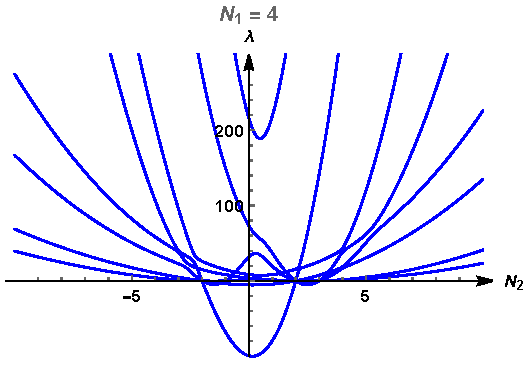
\includegraphics[width=0.45\textwidth]{\imagedir/eig1.pdf}
\hfill
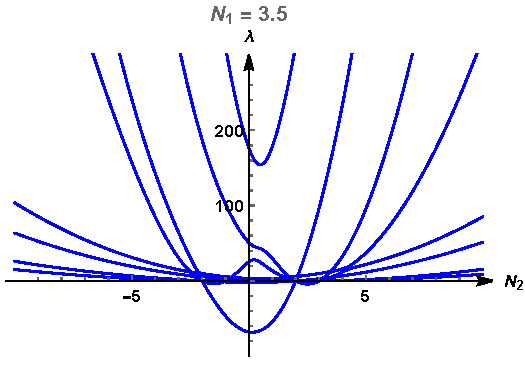
\includegraphics[width=0.45\textwidth]{\imagedir/eig2.pdf} \\

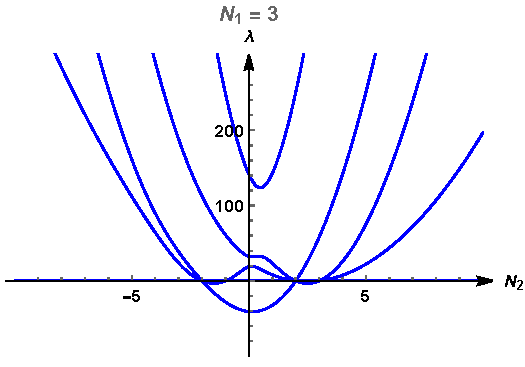
\includegraphics[width=0.45\textwidth]{\imagedir/eig3.pdf}
\hfill
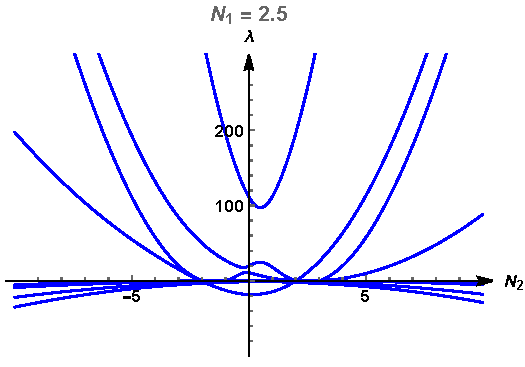
\includegraphics[width=0.45\textwidth]{\imagedir/eig4.pdf} \\

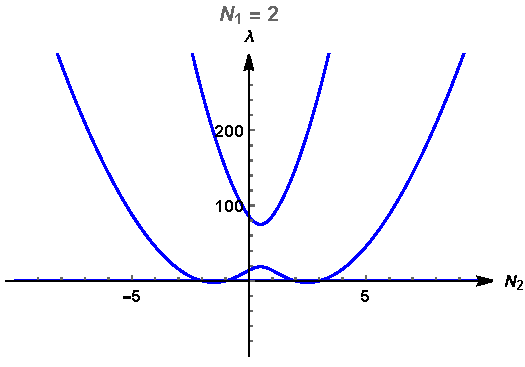
\includegraphics[width=0.45\textwidth]{\imagedir/eig5.pdf}
\hfill
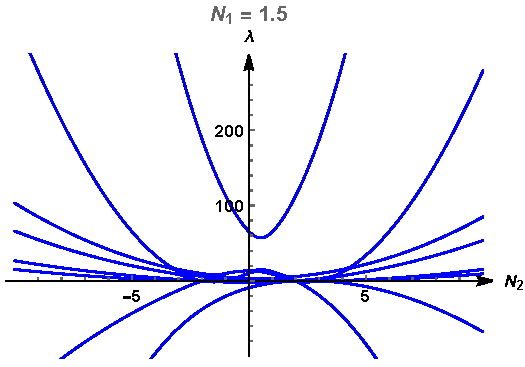
\includegraphics[width=0.45\textwidth]{\imagedir/eig6.pdf} \\

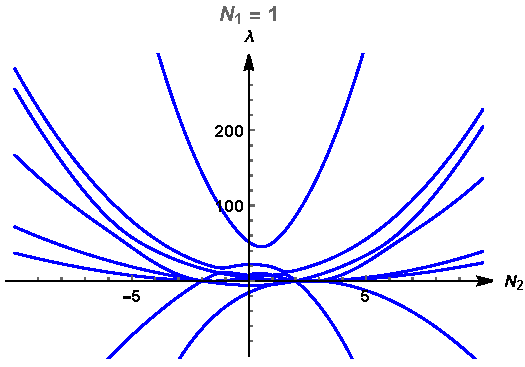
\includegraphics[width=0.45\textwidth]{\imagedir/eig7.pdf}
\hfill
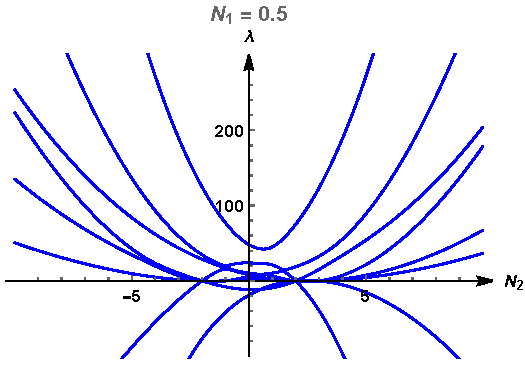
\includegraphics[width=0.45\textwidth]{\imagedir/eig8.pdf}

\caption{Eigenvalues of the Zamolodchikov metric at various values of $N_1$ and $N_2$.}
\label{Eigenvalues}
\end{figure}

\noindent When $-2 < N_1 < 3$ or $-2 < N_2 < 3$, the metric has both positive and negative eigenvalues. If $N_1$ and $N_2$ are each greater than 3 or less then $-2$, it is positive-definite. In \cref{Eigenvalues} we plot the eight eigenvalues of the Zamolodchikov metric for various values of $N_1$ and $N_2$. In general it is not possible to provide closed-form expressions for the eigenvalues, since they are roots of an eigth-order polynomial. An exception occurs at $N_1=2$, where six eigenvalues equal zero, while the remaining two are given by
\begin{align}
\lambda_\pm = \frac{100-25N_2+25N_2^2}{2}
\pm \frac{5}{2}\sqrt{208-328N_2+337N_2^2-18N_2^3+9N_2^4}\,.
\end{align}



\section{Reduced Equations on the Central Manifold}
\label{appendix:normalForm}
In this appendix we derive the reduced equations on the parameter-dependent center manifold of the system of ordinary differential equations given by
\begin{equation} \label{rgflow:eq:ODE}
    \dot g_i = \beta_i(\vec{g}, \vec{\alpha}) = -g_i + \beta^{(2)}_i(\vec g, \vec \alpha)\,,
\end{equation}
at the (numerically derived) zero-Hopf point located at $\alpha^* = (N_1^*, N_2^*)$, see \cref{eq:ZH}. Here the functions $\beta^{(2)}$ are listed in \crefrange{eq:beta1}{eq:beta8} and depend on the vector-valued function $\vec{g} \colon \mathbb R \rightarrow \mathbb R^8$ and the vector $\vec{\alpha}\textbf{} = (N_1,N_2) \in \mathbb R^2$. For brevity of notation, we use units where $\epsilon=1$. The analysis is general and applies to any 2-parameter dynamical system exhibiting a ZH bifurcation. For readability, all calculations will be rounded up to four figures 
from here on out, although to reproduce the figures in \cref{sec:QFT} it is necessary to work at significantly higher precision. The derivation of the normal form is also carefully worked out in the textbook \cite{Guao2013BifurcationTheory}, see also \cite{Kuznetsov2004}.

First, we translate the bifurcation point to the origin by introducing
new variables $\bar g \equiv \vec g - g^\ast$ and parameters $\bar \alpha \equiv \vec \alpha -
\alpha^\ast$. We immediately drop the bars again for readability. Thus, the
ZH point is now located at $(\vec{g}, \vec{\alpha}) = (0,0) \in \mathbb
R^{8 + 2}$. The right-hand side of \cref{rgflow:eq:ODE} can be expanded as
\begin{equation}
\label{eq:Fexpansion}
\begin{aligned}
    \beta(\vec{g}, \vec{\alpha}) =& 
    A\vec g + B(\vec{g},\vec{\alpha}) = \mathcal \beta_{0,1} (\vec{\alpha}) 
    + \frac12 \mathcal \beta_{2,0}(\vec g,\vec g) + \mathcal \beta_{1,1}(\vec g,\vec \alpha) 
    + \frac12 \mathcal \beta_{0,2}(\vec \alpha,\vec \alpha)  \\
    &  + \frac12 \mathcal \beta_{2,1}(\vec g,\vec g,\vec \alpha)
       + \frac12 \mathcal \beta_{1,2}(\vec g, \vec \alpha, \vec \alpha) 
       + \frac16 \mathcal \beta_{0,3}(\vec \alpha,\vec \alpha,\vec \alpha) + \cdots,
\end{aligned}
\end{equation}
where $A_{ij} =\partial_{g_i} \beta^j(\vec g,\vec \alpha)$ is the Jacobian of $\beta^j(\vec g,\vec \alpha)$ at the ZH point, 
the notation $\beta_{i,j}$ means that we expand to the $i^{\text{th}}$ order in coupling constant and to the $j^{\text{th}}$ order in parameters
\begin{multline}
   \mathcal \beta_{i,j}(\vec{g}_1, \vec{g}_2, \cdots, \vec{g}_i, \vec{\alpha}_1, \vec{\alpha}_2 \cdots, \vec{\alpha}_j)  \\
    = \frac{\partial^i}{\partial t_1 \partial t_2 \dots \partial t_i}
      \frac{\partial^j}{\partial s_1 \partial s_2 \dots \partial s_j}
        \left. \beta\left(\sum_{r=0}^i t_r \vec{g}_r,  \sum_{r=0}^j s_r \vec{\alpha}_r\right) 
            \right\vert_{t_r=s_r=0}.
\end{multline}
Note that we did not include the multilinear form $\mathcal \beta_{3,0}$ in
\cref{eq:Fexpansion} since it is identically zero in the perturbative approximation we are working at, where $\beta(g,\alpha)$ is only computed up to second order in the coupling constants. Now we truncate the expansion \cref{eq:Fexpansion} at the third order in the sum $I=i+j\leq 3$. The reason we perform this double expansion and truncate parameters and couplings together is that we are interested in RG trajectories near the ZH point that do not run away but exhibit fluctuations in coupling space that scale with the magnitude of $\vec{\alpha}$.

To confirm that the point under consideration is indeed a ZH point we
inspect the eigenvalues of the linearization of \cref{rgflow:eq:ODE} at
\cref{eq:ZH}, i.e., the eigenvalues of the matrix $A$. This set can be divided
into three parts
\begin{align*}
    \sigma_s &= 
\left\{
    \num{-0.48779687722209303}, \;
    \num{-0.22070478585058576}, \;
    \num{-0.11374063283553064}
\right\}, \,
    \sigma_c = 
\left\{
   \pm 0.02756 i,\;
    0
\right\}, \,
    \sigma_u = 
\left\{
    \num{0.40013960733401366}, \;
    1
\right\},
\end{align*}
corresponding to the UV-stable, center, and UV-unstable eigenspaces of $A$, respectively. The eigenvalue $1$ is exact at second order in perturbation theory and owes to the homogeneity of $\beta+g$ \cite{Jepsen:2020czw}. 
As a shorthand we introduce $\omega = 0.02756$.
Then, since the eigenvalues in $\sigma_c$ are non-degenerate or simple, there are eigenvectors $p_0\in
\mathbb R^8$ and $p_1 \in \mathbb C^8$, and adjoint eigenvectors $q_0\in \mathbb R^8$
and $q_1 \in \mathbb C^8$ such that the following relations hold
\begin{equation} \label{rgflow:eq:eigenvectors}
    A q_0 = 0, \quad A q_1 = i \omega q_1, \quad A \bar{q}_1 = - i \omega \bar{q}_1, 
    \quad A^T p_0 = 0, \quad A^T p_1 = -i \omega p_1, \quad A^T \bar{p}_1= i \omega \bar{p}_1 \,.
\end{equation}
Furthermore, letting $\braket{a,b} = a^\dagger b$, the eigenvectors can be normalized such that
\begin{equation} \label{eq:normalization}
    \left< p_0, q_0 \right> = \left< p_1, q_1 \right> = \left< \bar{p}_1, \bar{q}_1 \right> =1 %, \notag\\
\end{equation}
while the other scalar products vanish, thus $\braket{p_1,q_0} = \braket{p_1,\bar{q}_1} = 0$. Specifically, we may choose
\begin{gather}
    q_0 =
    \begin{pmatrix*}[r]
        \num{-0.024962045785115454}\\
        \num{-0.10198878031459158}\\
        \num{0.1370967174936959}\\
        \num{-0.18189204279387905}\\
        \num{0.10357353240934195}\\
        \num{0.39482963902880625}\\
        \num{0.386794832337773}\\
        \num{-0.7879510117934457}
    \end{pmatrix*}, \hspace{20mm}
    q_1 = \begin{pmatrix*}[r]
        \num{ 0.02737513360232479 - 0.003733614980153608i} \\
        \num{ 0.09744013935416052 - 0.0020530876830862745i} \\
        \num{-0.13774705391103442 + 0.00807224514050541i} \\
        \num{ 0.13175352387314418 + 0.07592000338211646i} \\
        \num{-0.10458024483382158 + 0.009853089597229372i} \\
        \num{-0.34394317550947723 - 0.06262404784966186i} \\
        \num{-0.3981806627081541  - 0.03840975492368228i} \\
        \num{ 0.8088879258111088  }
    \end{pmatrix*},
\end{gather}
and
\begin{gather}
    p_0 =
        \begin{pmatrix*}[r]
        0\\
        \num{290.40443359353833}\\
        \num{-27.716162413627636}\\
        \num{222.0377118032486}\\
        \num{197.5427565762014}\\
        \num{246.85342933411596}\\
        \num{65.72788403238042}\\
        \num{86.9898946889358}
    \end{pmatrix*}, \hspace{20mm}
    p_1 = \begin{pmatrix*}[r]
        0\\
        \num{134.55856247086953 + 29.9173893182363i} \\
        \num{-12.377125600554889 - 31.10832072754824i} \\
        \num{102.46219419760145 + 19.8244601587464i} \\
        \num{96.22303233249862 + 34.468566651217735i} \\
        \num{114.25684023697899 + 21.677063687988955i} \\
        \num{31.128205370978275 - 8.470440147865185i} \\
        \num{41.95818021284129 - 2.6264860002350456i}
    \end{pmatrix*}.
\end{gather}
Note that the above normalization does not uniquely define the eigenvectors.
For example, we can scale $(p_0, q_0) \rightarrow (c p_0, \frac1c q_0)$ for $c\neq 0$ while leaving
\cref{rgflow:eq:eigenvectors} and \cref{eq:normalization} invariant.

To write the equations below in a compact form it is
convenient to introduce the matrices $\Phi = \left( q_0\; q_1\; \bar q_1
\right)$ and $\Psi = \left( p_0\; p_1\; \bar p_1 \right )$. Due to
the normalization \cref{eq:normalization}, we have the identity $\left< \Psi,
\Phi \right> = \Psi^\dagger \Phi = I_3$, where $I_n$ is the $n\times n$ identity matrix. Moreover $P_c = \Phi \Psi^\dagger$ is a projector on the center subspace: $P_c^2=P_c$. Right at $\alpha = 0$ there exists a unique manifold tangent to $q_0$, $q_1$, and $\bar q_1$. For non-zero $\alpha$ this manifold can be continued into a one-parameter family of three-dimensional invariant manifolds known as the center manifold. Any real vector $\vec{g}\in\mathbb R^8$ that belongs to the central manifold can be represented as
\begin{equation}
    \vec{g} = x q_0 + z q_1 + \bar z \bar q_1 + w(x,z,\bar{z},\alpha\textbf{}),
\end{equation}
where $x=\left< p_0, g \right>\in\mathbb R$,
$z=\left< p_1, g \right>\in\mathbb C$, and $\left< p_j, w \right> = 0$ for $j=0,1$. The time derivatives of $x$ and $z$ are given by
\begin{equation} \label{eq:reducedsystem_complex_form}
    \begin{cases} 
    \begin{aligned}
        \dot x(t) &{}= f^0(x,z,\bar z, \alpha), \\
        \dot z(t) &{}= %i \omega z(t) + 
        f^1(x,z,\bar z, \alpha),
    \end{aligned}  
    \end{cases} 
\end{equation}
where 
\begin{equation} \label{eq:gj}
f^j(x,z,\bar z, \alpha) = \bar p_j \beta\textbf{}\Big(x q_0 + z q_1 + \bar{z} \bar{q}_1 + w(x,z,\bar z, \alpha) , \alpha\Big)\,, \qquad j=0,1.
\end{equation}
Meanwhile, $w$ cannot be an arbitrary function of its arguments but must satisfy the differential equation
\begin{equation} \label{eq:wdot}
    \dot w = %Aw + 
    \left( I_8 -  P_c \right)\beta\Big(x q_0 + z q_1 + \bar{z}\bar{q}_1 + w(x,z,\bar z, \alpha) , \alpha\Big)\,.
\end{equation}
Next we expand the mappings $f^0, f^1$ and $w$ as follows
\begin{equation}
\begin{aligned}
f^0(x,z,\bar z, \alpha) 
=& \sum f^0_{ijklm} x^i z^j \bar{z}^k    \alpha_1^l \alpha_2^m   \\
= &\,
f^0_{00010} \alpha_1 + f^0_{00001} \alpha_2 + \frac12 f^0_{200} x^2 + \Re \left(f^0_{020} z^2 \right) + f^0_{011} z\bar z + 2 x \Re \left( f^0_{110} z \right)   \\
   &+  f^0_{10010} x \alpha_1 + f^0_{10001} x \alpha_2 + \frac16 f^0_{300} x^3 + f^0_{111} x |z|^2 +  x^2 \Re \left( f^0_{210} z \right),  \\
   &+ |z|^2 \Re \left( f^0_{021} z \right)     \vspace{2mm}  \\
f^1(x,z,\bar z, \alpha) =& \sum g^1_{ijklm} x^i z^j \bar{z}^k   \alpha_1^l \alpha_2^m   \\
=&\, i \omega z+ f^1_{00010} \alpha_1 + f^1_{00001} \alpha_2 + \frac12 f^1_{200} x^2 + \frac12 f^1_{020} z^2 + \frac12 f^1_{002} \bar z^2 + f^1_{011} |z|^2   \\
    & + f^1_{110} x z + f^1_{101} x \bar z + f^{1}_{01010} z \alpha_1 + f^{1}_{01001} z \alpha_2 + \frac16 f^1_{300} x^3 +
        f^1_{111} x |z|^2  \\
    &+ \frac12 f^1_{210} x^2 z + \frac12 f^1_{021}  z |z|^2,
    \\
w(x,z,\bar z, \alpha) =& \sum w_{ijklm} x^i z^j \bar{z}^k  \alpha_1^l \alpha_2^m   \label{eq:w} \\
= &\, w_{00010} \alpha_1 + w_{00001} \alpha_2 + \frac12 w_{200} x^2 + 2 \Re\left(w_{110} xz \right) +  w_{011} z\bar z + \Re\left( w_{020} z^2 \right), 
\end{aligned}
\end{equation}
where $f^{0,1}_\mu \in \mathbb C$ and $w_\nu \in \mathbb C^8$,
with multi-indices $\mu$ and $\nu$ parametrizing the degrees of expansion in couplings and in parameters. We also used an abbreviated notation where $f^{0,1}_{ijk} = f^{0,1}_{ijk00}$. Since $f^0$ is a real-valued
function, we have the identities $f^0_{ijkmn} = \bar f^0_{ikjmn}$ and 
$f^0_{ijjmn} \in \mathbb R$. Since $w$ is also a real-valued function, the
same symmetry holds for the coefficients of $w$.  


Comparing the equation \cref{eq:gj} and \cref{eq:Fexpansion} we can fix the coefficients in \cref{eq:w}:
\begin{align*}
    f^j_{200} &{}= \bar{p}_j \cdot \beta_{2,0}(q_0, q_0),
        &f^j_{110} &{}= \bar{p}_j \cdot \beta_{2,0}(q_0, q_1),
        &f^j_{020} &{}= \bar{p}_j \cdot \beta_{2,0}(q_1, q_1), \\
    f^j_{002} &{}= \bar{p}_j \cdot \beta_{2,0}(\bar q_1, \bar q_1),
        &f^j_{101} &{}= \bar{p}\textbf{}_j \cdot \beta_{2,0}(q_0, \bar q_1),
\end{align*}
for $j=0,1$. And
\begin{equation}
    f^j_{00010} \alpha_1 + f^j_{00001} \alpha_2 = \bar{p}_j \cdot \beta_{0,1} \alpha\,, \qquad j=0,1,
\end{equation}
For the higher order parameter-dependent terms $f^j_{10010}$ and $f^j_{10001}$ could be computed in a similar way.
Then we decompose $z = u + iv$, with $u$ and $v$ real, in \cref{eq:reducedsystem_complex_form} to obtain the three-dimensional real system given by
\begin{equation} \label{eq:reducedsystem}
\begin{aligned}
    \dot x ={}& p_0 \cdot \beta_{0,1}\alpha + \frac12 f^0_{200} x^2 + f^0_{011} (u^2+v^2) + 2 (\Re(f^0_{110}) u - \Im(f^0_{110})) v x + \Re(f^0_{020}) (u^2-v^2) - \\
                    & 2\Im(f^0_{020}) u v + \Re(f^0_{10010}) x \alpha_1 + \Re(f^0_{10001}) x \alpha_2 + \frac16 f^0_{300} x^3 + \Re(f^0_{210}) u x^2 - \Im(f^0_{210}) v x^2 \\ 
                    & + \Re(f^0_{021}) u (u^2+v^2) - \Im(f^0_{021}) v (u^2+v^2) + \Re(f^0_{111}) x (u^2+v^2), \\
    \dot u ={}&  -\omega v + \Re (p_1) \cdot \beta_{0,1}\alpha + \frac12 \Re(f^1_{200}) x^2 + \frac12 (\Re(f^1_{020}) +  \Re(f^1_{002})) (u^2-v^2) + \\
                    & (\Im(f^1_{002}) -  \Im(f^1_{020})) u v + (\Re(f^1_{110}) +  \Re(f^1_{101})) x u + (\Im(f^1_{101}) - \Im(f^1_{110})) v x + \\
                    & \Re(f^1_{011}) (u^2+v^2) + \Re(f^1_{01010}) u \alpha_1 - \Im(f^1_{01010}) v \alpha_1 + \Re(f^1_{01001}) u \alpha_2 - \Im(f^1_{01001}) v \alpha_2 + \\
                    & \frac16 \Re(f^1_{300}) x^3 + \frac12 \Re(f^1_{210}) x^2 u - \frac12 \Im(f^1_{210}) x^2 v + \frac12 \Re(f^1_{021}) u (u^2+v^2) - \\
                    & \frac12 \Im(f^1_{021}) v (u^2+v^2) + \Re(f^1_{111}) x (u^2+v^2), \\
    \dot v ={}&   \omega u +  \Im (p_1) \cdot \beta_{0,1}\alpha+ \frac12 \Im(f^1_{200}) x^2 + \frac12 (\Im(f^1_{020}) +  \Im(f^1_{002})) (u^2-v^2) + \\ 
                    & (\Re(f^1_{020}) -  \Re(f^1_{002})) u v + (\Im(f^1_{110}) +  \Im(f^1_{101})) x u + (\Re(f^1_{110}) - \Re(f^1_{101})) x v + \\
                    & \Im(f^1_{011}) (u^2+v^2) + \Im(f^1_{01010}) u \alpha_1 + \Re(f^1_{01010}) v \alpha_1 + \Im(f^1_{01001}) u \alpha_2 + \Re(f^1_{01001}) v \alpha_2 +  \\
                    & \frac16 \Im(f^1_{300}) x^3 + \frac12 \Im(f^1_{210}) x^2 u + \frac12 \Re(f^1_{210}) x^2 v + \frac12 \Im(f^1_{021}) u (u^2+v^2) + \\
                    & \frac12 \Re(f^1_{021}) v (u^2+v^2) + \Im(f^1_{111}) x (u^2+v^2)\,.
\end{aligned}
\end{equation}
The truncated normal form \cref{eq:ZHnormform} exhibits a rotational symmetry in the $(u,v)$-plane. This symmetry is not a symmetry of the full system. Consequently, the approximation $\cref{eq:ZHnormform}$ misrepresents essential qualitative properties of the RG flow around the bifurcation point. For this reason we retained cubic terms in the above expansions so that the symmetry is broken. Incidentally, the cubic terms are non-resonant, meaning that one could get rid of them by a suitable change of variables and thereby restore the $(u,v)$ rotation symmetry at cubic order.  But in doing so, one generates new symmetry-breaking terms at higher order. In principle, one could retain the symmetry at any desired order by iterating this procedure, but retaining the symmetry at all orders requires a singular change of variables.
\end{subappendices}


%% Discussion
\chapter{Concluding remarks}
\epigraph{ ``Solving intelligence, and then using that to solve everything
else.''}{{\it Demis Hassabis}}
At this stage we have robust predictors for switching to  non-hyperbolic cycles
emanating from generalized Hopf, fold-Hopf, transcrical-Hopf, and Hopf-Hopf
bifurcation points, and also to homoclinic orbits emanating from generic and
transcritical codimension two Bogdanov--Takens bifurcation points in classical
DDEs. The implementation in \DDEBIFTOOL provides a powerful tool to analyze
discrete delay differential equations. The next obvious step is to generalize
\cite{Kuznetsov2005,DeWitte2013,DeWitte2014} by deriving normal forms for
bifurcation of periodic orbits for DDEs. As announced in the introduction, we
already made great progress on this problem and expect to publish our results
soon.

At times, it felt somewhat redundant working with the numerical software packages
\DDEBIFTOOL and \MATCONT. Indeed, a large part of the code to initialize the
homoclinic predictors is identical in both software packages. We therefore
believe it would be beneficial to merge these two separate software packages into
one larger package. At the time, \MATLAB was the obvious programming environment
for those packages to be coded in. It could run on multiple hardware
architectures and operating systems. Additionally, the scripting language makes
is easy for students to participate in the projects, without having to have a
deep understanding of programming. However, in our opinion, Julia would be the
more suitable choice now. Indeed, next to the benefits mentioned above for
\MATLAB, Julia supports multiple-dispatch, is very fast (you don't need to
vectorize your code in order to obtain speed as in MATLAB), it is freely
available, and has a great community and rapidly growing ecosystem. With a focus
on large scale systems, there is already the Julia package
\texttt{BifurcationKit.jl} \cite{veltz:hal-02902346}. We
envision this package to grow to support a graphical user interface, as in
\MATCONT, and to be able to analyze delayed systems as in \DDEBIFTOOL.

A question that remains open, is what the exact radius of convergence of the
homoclinic asymptotic near the generic quadratic codimension two Bogdanov-Takens
bifurcation  point is. Peter de Maesschalck began looking into this and has
already found some promising results. This may then be used to expand the radius
of convergence for example. The same type of problem arises when studying
homocinic and heteroclinic orbits in the degenerated Bogdanov--Takens
bifurcations of Bogdanov--Takens bifurcation with symmetries, see for example
\cite{chow_li_wang_1994}. It would be interesting to study these problems as
well. 

On a related note, we would like to revisit the problem of obtaining homoclinic
asymptotics near the zero-Hopf point. It was all but trivial to locate the
homoclinic order in the chaotic bi-antisymmetric tensor model.

Lastly, the rapid growth of artificial intelligence seems to be able to solve
more and more problems every day. This also applies to the field of mathematics,
see for example \cite{Davies2021}, and \cite{631606893d774be2a2c919789d14b2d6}.
We therefore wonder --- ``Would it be possible to obtain a homoclinic predictor
near the generic codimension two Bogdanov--Takens bifurcation in infinite
dimensional systems generated by DDEs training a neural network?''.


\bibliographystyle{siamplain}
\bibliography{references}

\end{document}
